\appendix
\addcontentsline{toc}{chapter}{LAMPIRAN}

% --- LAMPIRAN I ---
\refstepcounter{chapter} 
\renewcommand{\thechapter}{\Roman{chapter}}
\addcontentsline{toc}{section}{Lampiran \thechapter\ Dataset}
\noindent{\large Lampiran \thechapter\ Dataset} \par
\vspace{0.5cm}

Penelitian ini menggunakan data sekunder dari laporan Survei Status Gizi Indonesia (SSGI) tahun 2024. Berikut adalah rincian akses data:

\begin{enumerate}
    \item \textbf{Sumber Data Mentah (Laporan Resmi):} \\
    \url{https://www.badankebijakan.kemkes.go.id/survei-status-gizi-indonesia-ssgi-2024/}
    
    \item \textbf{Draf Dataset Pra-pemrosesan:} \\
    \url{https://bit.ly/Dataset_SSGI_2024}
\end{enumerate}

Tabel berikut menyajikan daftar komprehensif 56 variabel independen yang diekstraksi dari laporan SSGI 2024 pada tahap awal sebelum dilakukan seleksi fitur. Penjelasan pada tabel ini merujuk pada distribusi kategori tematik yang sebelumnya dirangkum pada Bab 3.

\begin{longtable}{|c|p{0.30\textwidth}|p{0.35\textwidth}|p{0.25\textwidth}|}
    \caption{Daftar Lengkap Pemetaan 56 Variabel Determinan \textit{Stunting}}
    \label{table:lampiran_variabel}\\
    \hline
    \textbf{No} & \multicolumn{1}{c|}{\textbf{Kategori Tematik}} & \multicolumn{1}{c|}{\textbf{Nama Variabel (\textit{Fitur})}} & \multicolumn{1}{c|}{\textbf{Keterangan}} \tabularnewline 
    \hline
    \endfirsthead
    \hline
    \textbf{No} & \multicolumn{1}{c|}{\textbf{Kategori Tematik}} & \multicolumn{1}{c|}{\textbf{Nama Variabel (\textit{Fitur})}} & \multicolumn{1}{c|}{\textbf{Keterangan}} \tabularnewline 
    \hline
    \endhead
    \hline
    \endfoot
    \hline
    \endlastfoot
    
    1 & Riwayat Kehamilan dan Kelahiran & \texttt{persen\_\allowbreak jarak\_\allowbreak kehamilan\_\allowbreak berisiko} & Ibu hamil dengan jarak kehamilan terlalu dekat. \tabularnewline \hline
    2 & Riwayat Kehamilan dan Kelahiran & \texttt{persen\_\allowbreak usia\_\allowbreak ibu\_\allowbreak berisiko} & Ibu melahirkan di bawah usia 20 atau di atas 35 tahun. \tabularnewline \hline
    3 & Riwayat Kehamilan dan Kelahiran & \texttt{persen\_\allowbreak tidak\_\allowbreak ikut\_\allowbreak kelas\_\allowbreak bumil} & Ibu hamil yang tidak mengikuti kelas kehamilan. \tabularnewline \hline
    4 & Riwayat Kehamilan dan Kelahiran & \texttt{persen\_\allowbreak masalah\_\allowbreak buku\_\allowbreak kia} & Ibu yang memiliki kendala atau tanpa Buku KIA. \tabularnewline \hline
    5 & Riwayat Kehamilan dan Kelahiran & \texttt{persen\_\allowbreak kia\_\allowbreak tidak\_\allowbreak dijelaskan} & Memiliki Buku KIA namun tidak mendapat penjelasan medis. \tabularnewline \hline
    6 & Riwayat Kehamilan dan Kelahiran & \texttt{persen\_\allowbreak anc\_\allowbreak tidak\_\allowbreak lengkap\_\allowbreak k6} & Layanan \textit{Antenatal Care} (ANC) kurang dari 6 kali. \tabularnewline \hline
    7 & Riwayat Kehamilan dan Kelahiran & \texttt{persen\_\allowbreak anc\_\allowbreak tempat\_\allowbreak informal} & Pemeriksaan kehamilan dilakukan di fasilitas informal. \tabularnewline \hline
    8 & Riwayat Kehamilan dan Kelahiran & \texttt{persen\_\allowbreak usg\_\allowbreak tidak\_\allowbreak lengkap} & Ibu hamil dengan pemeriksaan USG tidak lengkap. \tabularnewline \hline
    9 & Riwayat Kehamilan dan Kelahiran & \texttt{persen\_\allowbreak usg\_\allowbreak oleh\_\allowbreak non\_\allowbreak spesialis} & Pemeriksaan USG dilakukan oleh tenaga non-spesialis. \tabularnewline \hline
    10 & Riwayat Kehamilan dan Kelahiran & \texttt{persen\_\allowbreak tidak\_\allowbreak patuh\_\allowbreak minum\_\allowbreak ttd} & Ibu hamil tidak patuh mengonsumsi Tablet Tambah Darah. \tabularnewline \hline
    11 & Riwayat Kehamilan dan Kelahiran & \texttt{persen\_\allowbreak mulai\_\allowbreak ttd\_\allowbreak terlambat} & Terlambat memulai konsumsi Tablet Tambah Darah (TTD). \tabularnewline \hline
    12 & Riwayat Kehamilan dan Kelahiran & \texttt{persen\_\allowbreak bblr} & Bayi lahir dengan status Berat Badan Lahir Rendah. \tabularnewline \hline
    13 & Riwayat Kehamilan dan Kelahiran & \texttt{persen\_\allowbreak pblr} & Bayi lahir dengan status Panjang Badan Lahir Rendah. \tabularnewline \hline
    14 & Riwayat Pemberian ASI dan MP-ASI & \texttt{persen\_\allowbreak imd\_\allowbreak terlambat} & Bayi yang terlambat menerima Inisiasi Menyusu Dini. \tabularnewline \hline
    15 & Riwayat Pemberian ASI dan MP-ASI & \texttt{persen\_\allowbreak tidak\_\allowbreak pernah\_\allowbreak asi} & Balita yang tidak pernah diberikan Air Susu Ibu (ASI). \tabularnewline \hline
    16 & Riwayat Pemberian ASI dan MP-ASI & \texttt{persen\_\allowbreak tidak\_\allowbreak asi\_\allowbreak eksklusif} & Bayi tidak mendapat ASI eksklusif selama 6 bulan penuh. \tabularnewline \hline
    17 & Riwayat Pemberian ASI dan MP-ASI & \texttt{persen\_\allowbreak diberi\_\allowbreak makanan\_\allowbreak campuran\_\allowbreak dini} & Makanan campuran diberikan sebelum sistem cerna siap. \tabularnewline \hline
    18 & Riwayat Pemberian ASI dan MP-ASI & \texttt{persen\_\allowbreak asi\_\allowbreak berhenti\_\allowbreak sebelum\_\allowbreak 2\_\allowbreak tahun} & Proses menyusui dihentikan sebelum anak berusia 2 tahun. \tabularnewline \hline
    19 & Riwayat Pemberian ASI dan MP-ASI & \texttt{persen\_\allowbreak mpasi\_\allowbreak tidak\_\allowbreak tepat\_\allowbreak waktu} & Makanan Pendamping ASI (MP-ASI) diberikan tidak tepat waktu. \tabularnewline \hline
    20 & Riwayat Pemberian ASI dan MP-ASI & \texttt{persen\_\allowbreak tidak\_\allowbreak memenuhi\_\allowbreak mdd} & Balita tidak memenuhi standar keberagaman makanan (MDD). \tabularnewline \hline
    21 & Riwayat Pemberian ASI dan MP-ASI & \texttt{persen\_\allowbreak tidak\_\allowbreak memenuhi\_\allowbreak mmf} & Balita tidak memenuhi frekuensi makan minimal (MMF). \tabularnewline \hline
    22 & Riwayat Pemberian ASI dan MP-ASI & \texttt{persen\_\allowbreak tidak\_\allowbreak memenuhi\_\allowbreak mmff} & Balita non-ASI dengan asupan susu kurang dari 2 kali/hari. \tabularnewline \hline
    23 & Riwayat Pemberian ASI dan MP-ASI & \texttt{persen\_\allowbreak tidak\_\allowbreak memenuhi\_\allowbreak mad} & Standar gizi \textit{Minimum Acceptable Diet} tidak terpenuhi. \tabularnewline \hline
    24 & Riwayat Pemberian ASI dan MP-ASI & \texttt{persen\_\allowbreak tidak\_\allowbreak konsumsi\_\allowbreak protein\_\allowbreak hewani} & Balita kurang mengonsumsi sumber protein hewani. \tabularnewline \hline
    25 & Riwayat Pemberian ASI dan MP-ASI & \texttt{persen\_\allowbreak konsumsi\_\allowbreak minuman\_\allowbreak manis} & Balita sering mengonsumsi minuman berpemanis. \tabularnewline \hline
    26 & Riwayat Pemberian ASI dan MP-ASI & \texttt{persen\_\allowbreak konsumsi\_\allowbreak makanan\_\allowbreak tak\_\allowbreak sehat} & Balita sering terpapar konsumsi makanan instan/kurang gizi. \tabularnewline \hline
    27 & Riwayat Pemberian ASI dan MP-ASI & \texttt{persen\_\allowbreak tidak\_\allowbreak konsumsi\_\allowbreak buah\_\allowbreak sayur} & Rendahnya tingkat konsumsi buah dan sayuran pada balita. \tabularnewline \hline
    28 & Riwayat Pemberian ASI dan MP-ASI & \texttt{persen\_\allowbreak pemberian\_\allowbreak makan\_\allowbreak dini} & Bayi diberikan makanan padat terlalu dini. \tabularnewline \hline
    29 & Riwayat Pemberian ASI dan MP-ASI & \texttt{persen\_\allowbreak diberi\_\allowbreak susu\_\allowbreak formula} & Balita mengonsumsi susu formula secara dominan. \tabularnewline \hline
    30 & Akses Pelayanan Kesehatan & \texttt{persen\_\allowbreak jarang\_\allowbreak pantau\_\allowbreak pertumbuhan} & Balita yang jarang dipantau pertumbuhannya di Posyandu. \tabularnewline \hline
    31 & Akses Pelayanan Kesehatan & \texttt{persen\_\allowbreak pemantauan\_\allowbreak nonstandar} & Pemantauan pertumbuhan tidak sesuai standar medis operasional. \tabularnewline \hline
    32 & Akses Pelayanan Kesehatan & \texttt{persen\_\allowbreak risiko\_\allowbreak layanan\_\allowbreak nonlengkap} & Balita menerima layanan fasilitas kesehatan tidak lengkap. \tabularnewline \hline
    33 & Akses Pelayanan Kesehatan & \texttt{persen\_\allowbreak tidak\_\allowbreak dapat\_\allowbreak pmt} & Balita/Bumil berisiko tidak menerima Pemberian Makanan Tambahan. \tabularnewline \hline
    34 & Akses Pelayanan Kesehatan & \texttt{persen\_\allowbreak pmt\_\allowbreak tidak\_\allowbreak habis} & Penerima tidak menghabiskan porsi Makanan Tambahan gizi. \tabularnewline \hline
    35 & Akses Pelayanan Kesehatan & \texttt{persen\_\allowbreak tidak\_\allowbreak dapat\_\allowbreak vit\_\allowbreak a} & Balita tidak mendapatkan suplementasi Vitamin A reguler. \tabularnewline \hline
    36 & Imunisasi dan Morbiditas Balita & \texttt{prevalensi\_\allowbreak underweight\_\allowbreak persen}* & Persentase balita dengan status gizi berat badan kurang. \tabularnewline \hline
    37 & Imunisasi dan Morbiditas Balita & \texttt{prevalensi\_\allowbreak wasting\_\allowbreak persen}* & Persentase balita dengan status gizi kurus akut. \tabularnewline \hline
    38 & Imunisasi dan Morbiditas Balita & \texttt{persen\_\allowbreak imunisasi\_\allowbreak dasar\_\allowbreak incomplete} & Balita tidak melengkapi jadwal imunisasi dasar. \tabularnewline \hline
    39 & Imunisasi dan Morbiditas Balita & \texttt{persen\_\allowbreak imunisasi\_\allowbreak lanjutan\_\allowbreak incomplete} & Balita tidak melengkapi jadwal imunisasi lanjutan. \tabularnewline \hline
    40 & Imunisasi dan Morbiditas Balita & \texttt{persen\_\allowbreak imunisasi\_\allowbreak pcv\_\allowbreak incomplete} & Balita tidak menerima vaksin PCV secara lengkap. \tabularnewline \hline
    41 & Imunisasi dan Morbiditas Balita & \texttt{persen\_\allowbreak imunisasi\_\allowbreak rotavirus\_\allowbreak incomplete} & Balita tidak menerima vaksin Rotavirus secara lengkap. \tabularnewline \hline
    42 & Imunisasi dan Morbiditas Balita & \texttt{persen\_\allowbreak balita\_\allowbreak ispa} & Persentase balita yang mengalami infeksi pernapasan (ISPA). \tabularnewline \hline
    43 & Imunisasi dan Morbiditas Balita & \texttt{persen\_\allowbreak balita\_\allowbreak diare} & Persentase balita yang mengalami kejadian diare rutin. \tabularnewline \hline
    44 & Imunisasi dan Morbiditas Balita & \texttt{persen\_\allowbreak balita\_\allowbreak pneumonia} & Balita yang terdiagnosis medis menderita pneumonia. \tabularnewline \hline
    45 & Imunisasi dan Morbiditas Balita & \texttt{persen\_\allowbreak balita\_\allowbreak tbc} & Balita yang terdiagnosis medis menderita tuberkulosis (TBC). \tabularnewline \hline
    46 & Kepemilikan Jaminan Kesehatan & \texttt{persen\_\allowbreak tidak\_\allowbreak memiliki\_\allowbreak jamkes} & Rumah tangga/anak tidak memiliki Jaminan Kesehatan Nasional. \tabularnewline \hline
    47 & Kepemilikan Jaminan Kesehatan & \texttt{persen\_\allowbreak jamkes\_\allowbreak tidak\_\allowbreak dimanfaatkan} & Fasilitas Jaminan Kesehatan dimiliki namun tidak dimanfaatkan. \tabularnewline \hline
    48 & Pendampingan dan Pengetahuan & \texttt{persen\_\allowbreak keluarga\_\allowbreak tanpa\_\allowbreak tpk} & Keluarga berisiko tidak didampingi Tim Pendamping Keluarga. \tabularnewline \hline
    49 & Pendampingan dan Pengetahuan & \texttt{persen\_\allowbreak balita\_\allowbreak dianggap\_\allowbreak berisiko} & Persepsi keluarga yang menganggap kondisi balitanya rentan. \tabularnewline \hline
    50 & Pendampingan dan Pengetahuan & \texttt{persen\_\allowbreak persepsi\_\allowbreak ibu\_\allowbreak anak\_\allowbreak bermasalah\_\allowbreak gizi} & Ibu menyadari anaknya mengalami permasalahan gizi klinis. \tabularnewline \hline
    51 & Pendampingan dan Pengetahuan & \texttt{persen\_\allowbreak pengetahuan\_\allowbreak stunting\_\allowbreak baik} & Tingkat pemahaman keluarga yang memadai mengenai \textit{stunting}. \tabularnewline \hline
    52 & Kontrasepsi Pasca Bersalin & \texttt{persen\_\allowbreak tidak\_\allowbreak kb\_\allowbreak pasca\_\allowbreak salin} & Ibu bersalin tidak menggunakan kontrasepsi pasca persalinan. \tabularnewline \hline
    53 & Bantuan Sosial & \texttt{persen\_\allowbreak tidak\_\allowbreak dapat\_\allowbreak bansos} & Keluarga sasaran tidak menerima Bantuan Sosial pemerintah. \tabularnewline \hline
    54 & Akses Air Minum dan Sanitasi & \texttt{persen\_\allowbreak akses\_\allowbreak air\_\allowbreak minum\_\allowbreak berisiko} & Rumah tangga dengan sumber air minum tidak layak/berisiko. \tabularnewline \hline
    55 & Akses Air Minum dan Sanitasi & \texttt{persen\_\allowbreak akses\_\allowbreak sanitasi\_\allowbreak berisiko} & Rumah tangga yang memiliki fasilitas sanitasi tidak layak. \tabularnewline \hline
    56 & Akses Air Minum dan Sanitasi & \texttt{persen\_\allowbreak pembuangan\_\allowbreak limbah\_\allowbreak berisiko} & Rumah tangga dengan sistem pembuangan limbah berisiko. \tabularnewline \hline
    
    \multicolumn{4}{p{\textwidth}}{\footnotesize \textit{*Catatan: Fitur prevalensi underweight dan wasting dieliminasi pada tahapan pra-pemrosesan model final (menyisakan 54 fitur) untuk menghindari terjadinya data leakage terhadap target probabilitas stunting.}} \tabularnewline
\end{longtable}

% --- LAMPIRAN II ---
\newpage
\refstepcounter{chapter} 
\addcontentsline{toc}{section}{Lampiran \thechapter\ Log Hasil Hyperparameter Tuning}
\noindent{\large Lampiran \thechapter\ Log Hasil Hyperparameter Tuning} \par
\vspace{0.5cm}

\begin{table}[H]
\centering
\caption{Log 10 Kombinasi Hyperparameter Terbaik Random Forest}
\label{tab:log_tuning}
\small
\resizebox{\textwidth}{!}{%
\begin{tabular}{|c|c|c|c|c|c|c|c|c|}
\hline
\textbf{No.} & \textbf{\textit{n\_estimators}} & \textbf{\textit{max\_depth}} & \textbf{\textit{min\_samples\_leaf}} & \textbf{\textit{max\_features}} & \textbf{Train MAE} & \textbf{Test MAE} & \textbf{Test RMSE} & \textbf{Rank} \\ \hline
1  & 100 & 5    & 1 & log2 & 1.3363 & 3.4378 & 3.4378 & 1 \\ \hline
2  & 150 & 5    & 1 & log2 & 1.3609 & 3.4883 & 3.4883 & 2 \\ \hline
3  & 100 & 5    & 2 & sqrt & 1.5093 & 3.5127 & 3.5127 & 3 \\ \hline
4  & 150 & 5    & 2 & log2 & 1.5617 & 3.5278 & 3.5278 & 4 \\ \hline
5  & 150 & 5    & 2 & sqrt & 1.4952 & 3.5299 & 3.5299 & 5 \\ \hline
6  & 100 & 7    & 2 & sqrt & 1.4897 & 3.5328 & 3.5328 & 6 \\ \hline
7  & 150 & 7    & 2 & log2 & 1.5378 & 3.5339 & 3.5339 & 7 \\ \hline
8  & 100 & None & 2 & sqrt & 1.4896 & 3.5347 & 3.5347 & 8 \\ \hline
9  & 150 & None & 2 & log2 & 1.5372 & 3.5352 & 3.5352 & 9 \\ \hline
10 & 150 & 7    & 2 & sqrt & 1.4776 & 3.5395 & 3.5395 & 10 \\ \hline
\end{tabular}%
}
\end{table}

\vspace{0.3cm}
\noindent\textit{Catatan: Angka performa pada baris pertama (Peringkat 1) merupakan parameter optimal yang dipilih dan digunakan sebagai model utama dalam penelitian ini. Riwayat lengkap dari seluruh 108 kombinasi parameter telah disimpan secara digital dalam file log\_hasil\_tuning.csv.}

% --- LAMPIRAN III ---
\newpage
\refstepcounter{chapter} 
\addcontentsline{toc}{section}{Lampiran \thechapter\ Nilai Rata-Rata Absolut SHAP (\textit{Feature Importance Plot})}
\noindent{\large Lampiran \thechapter\ Nilai Rata-Rata Absolut SHAP (\textit{Feature Importance Plot})} \par
\vspace{0.5cm}

\begin{figure}[H]
    \centering
    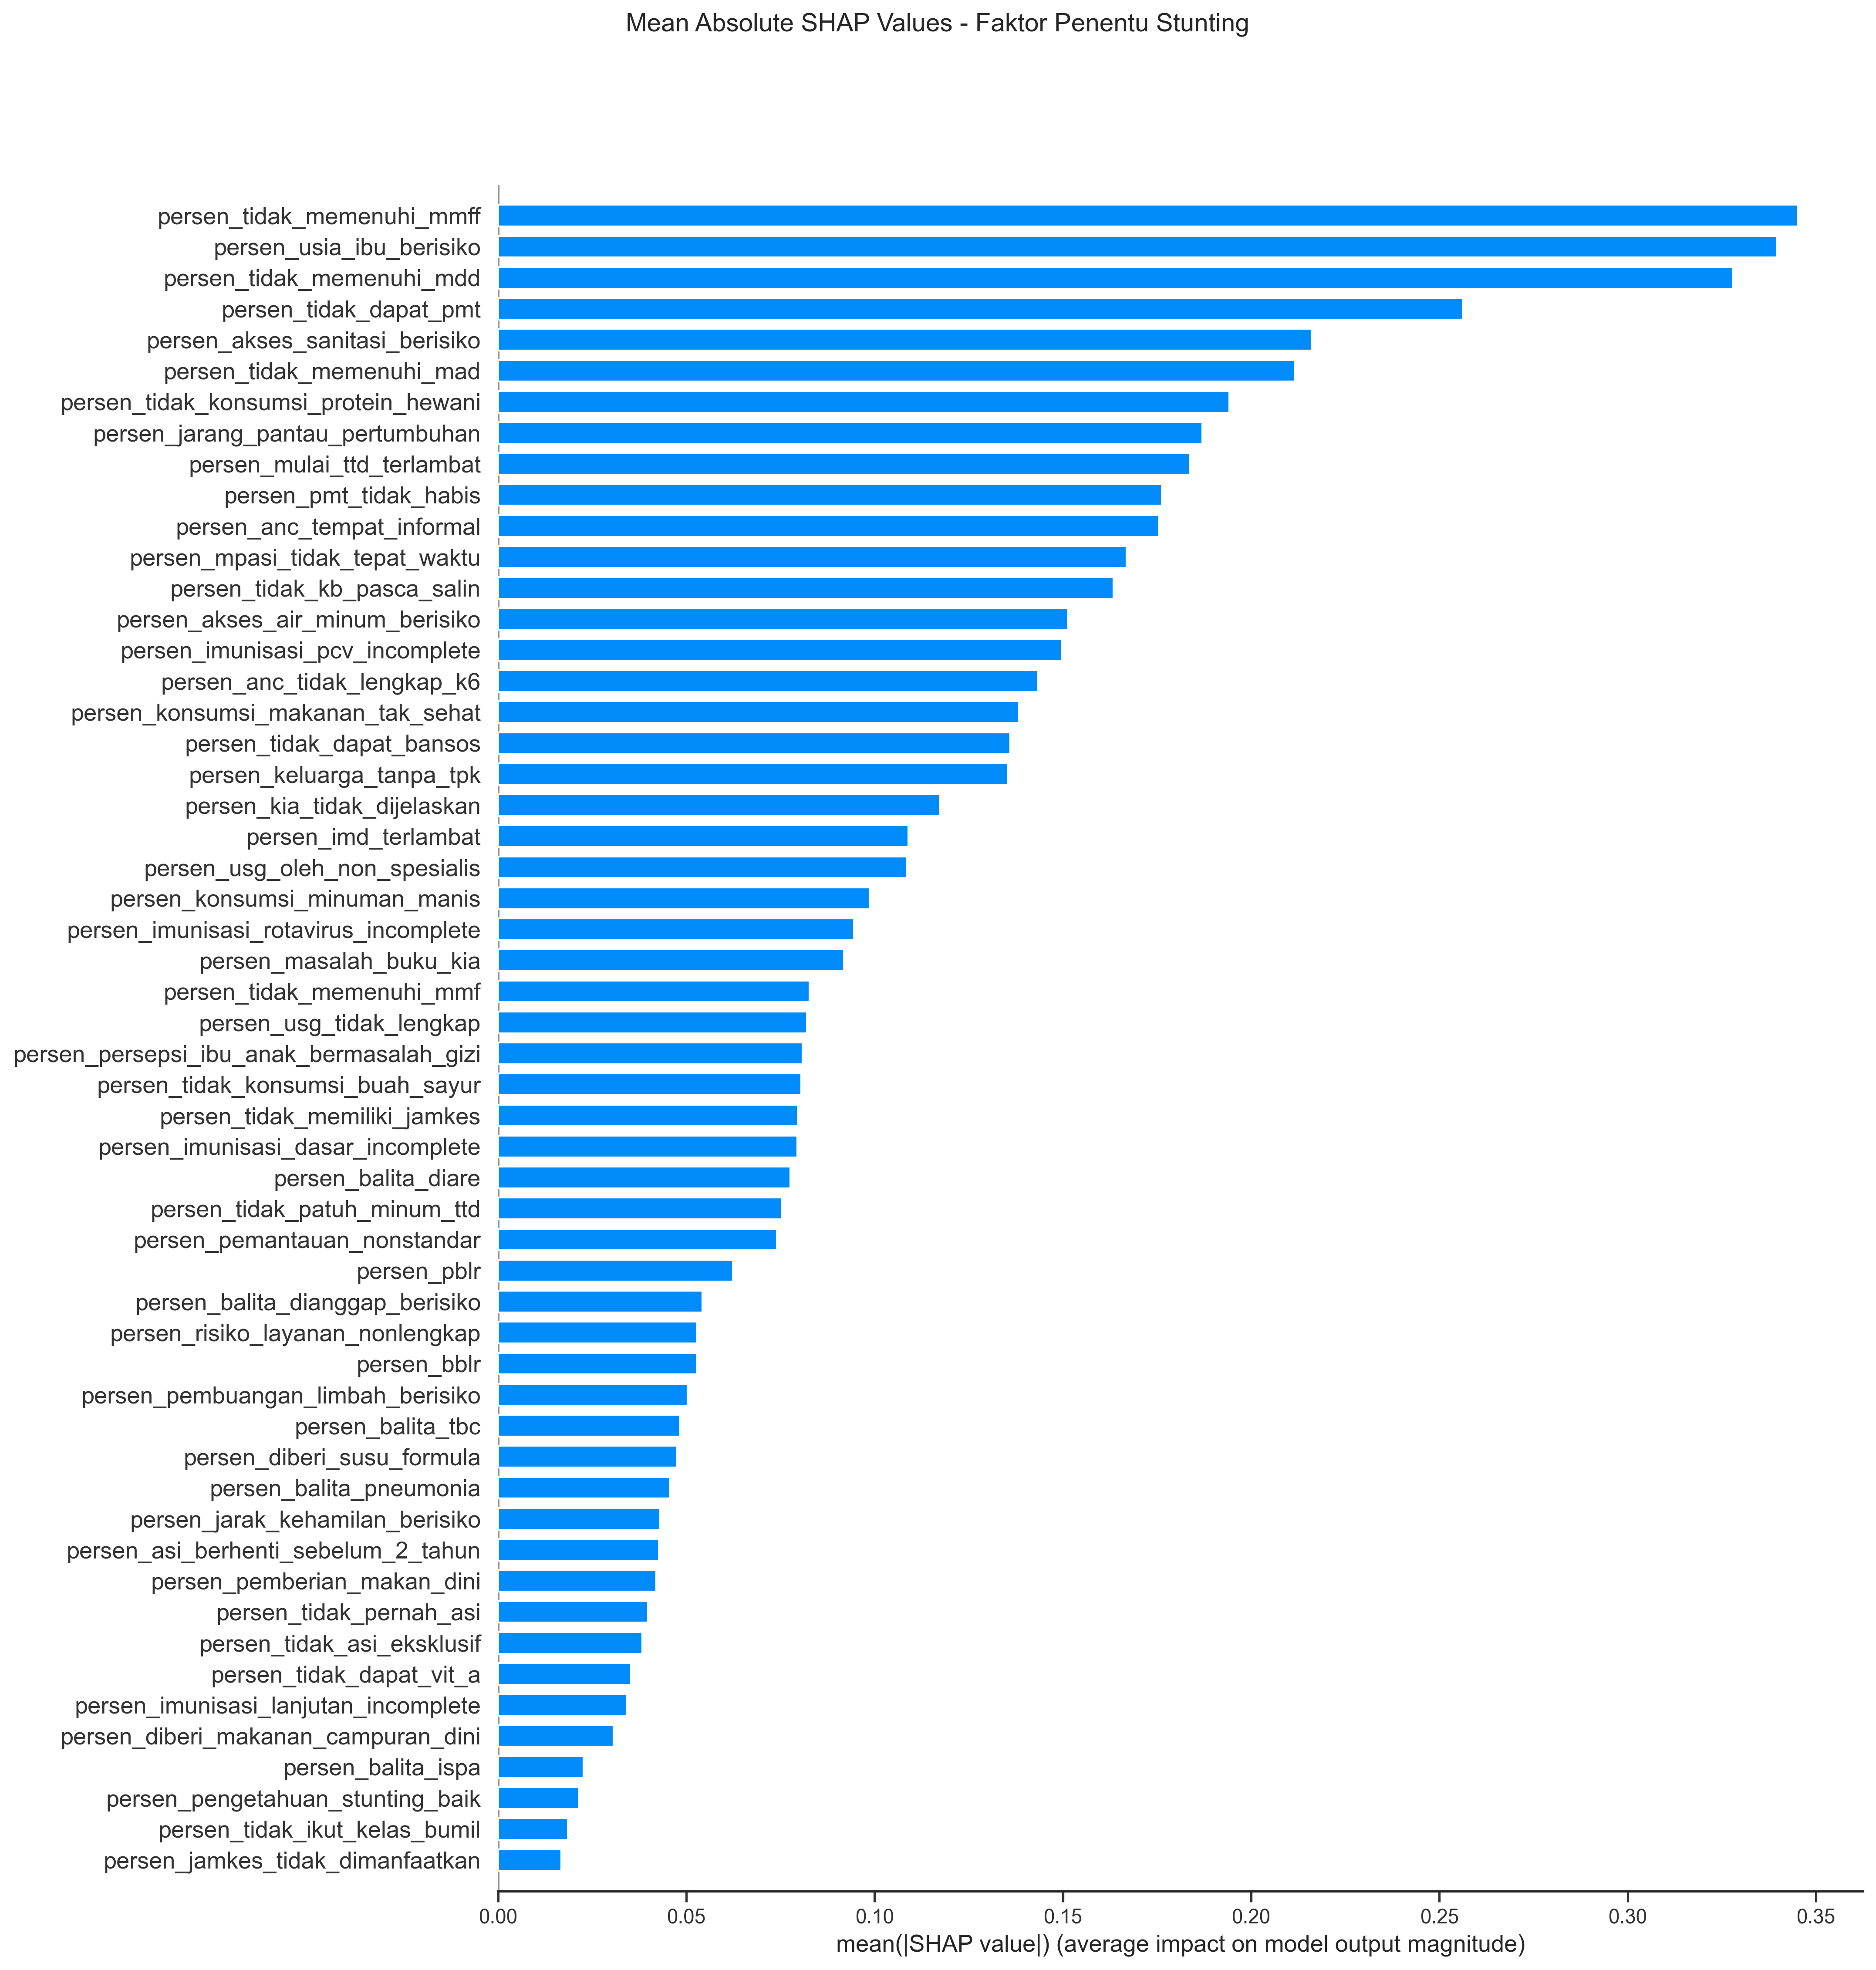
\includegraphics[width=0.9\textwidth]{figure/feature_importance_lengkap.png}
    \caption{Grafik Nilai Rata-Rata Absolut SHAP Seluruh Fitur}
\end{figure}

% --- LAMPIRAN IV ---
\newpage
\refstepcounter{chapter} 
\addcontentsline{toc}{section}{Lampiran \thechapter\ Arah dan Distribusi Dampak Fitur (\textit{SHAP Summary Plot})}
\noindent{\large Lampiran \thechapter\ Arah dan Distribusi Dampak Fitur (\textit{SHAP Summary Plot})} \par
\vspace{0.5cm}

\begin{center}
    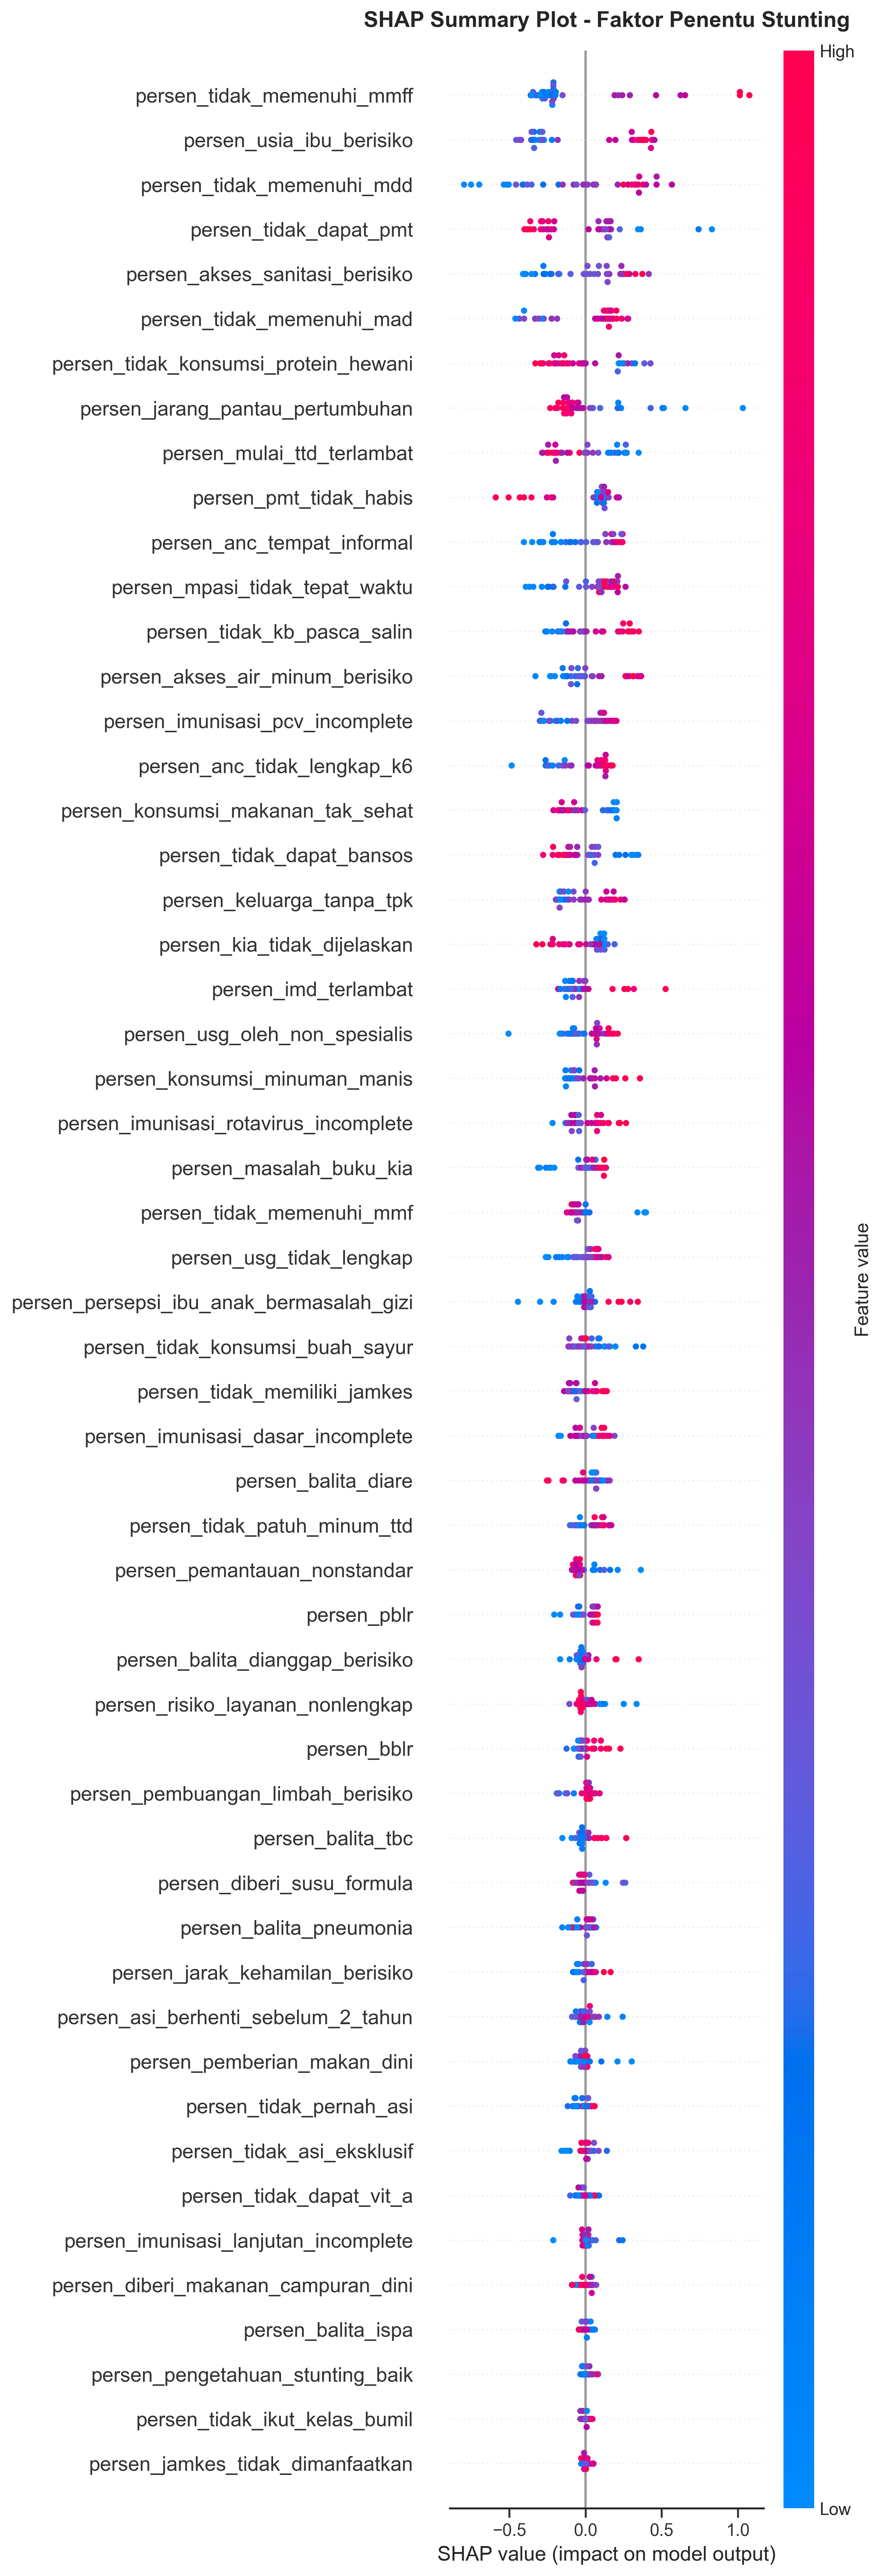
\includegraphics[width=0.5\textwidth]{figure/summary_plot_lengkap.png}
\end{center}

% --- LAMPIRAN V ---
\newpage
\refstepcounter{chapter} 
\addcontentsline{toc}{section}{Lampiran \thechapter\ Grafik Interaksi Fitur (\textit{SHAP Dependence Plot})}
\noindent{\large Lampiran \thechapter\ Grafik Interaksi Fitur (\textit{SHAP Dependence Plot})} \par
\vspace{0.5cm}

% HALAMAN 1 (8 GAMBAR)
\begin{figure}[H]
    \centering
    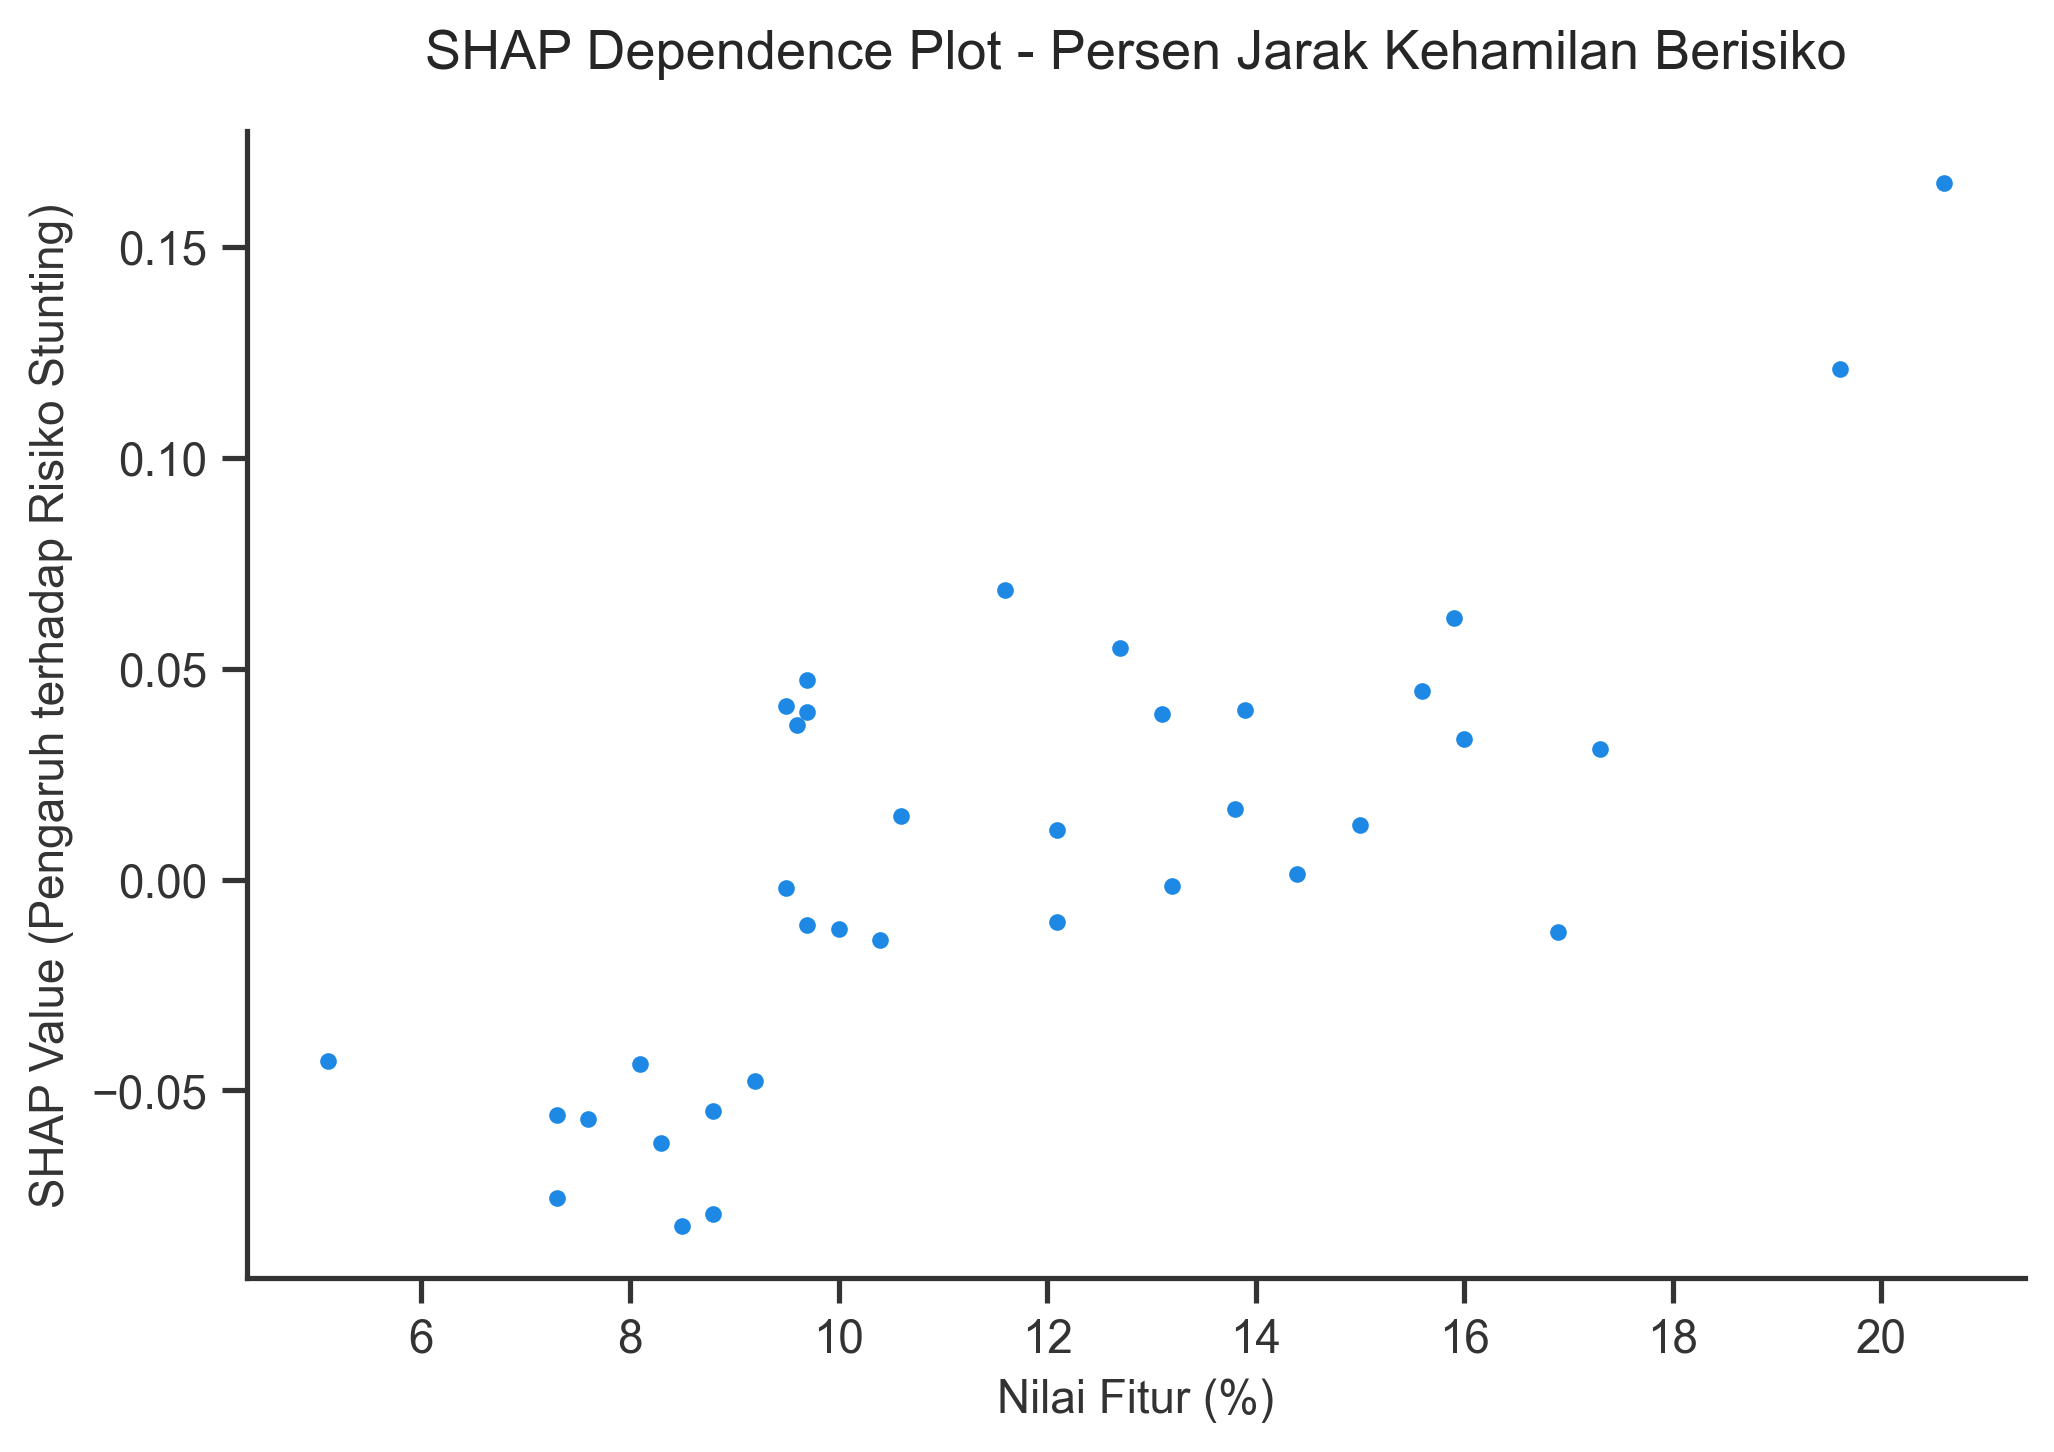
\includegraphics[width=0.48\textwidth]{figure/hasil_dependence_plot/dependence_persen_jarak_kehamilan_berisiko.png} \hfill
    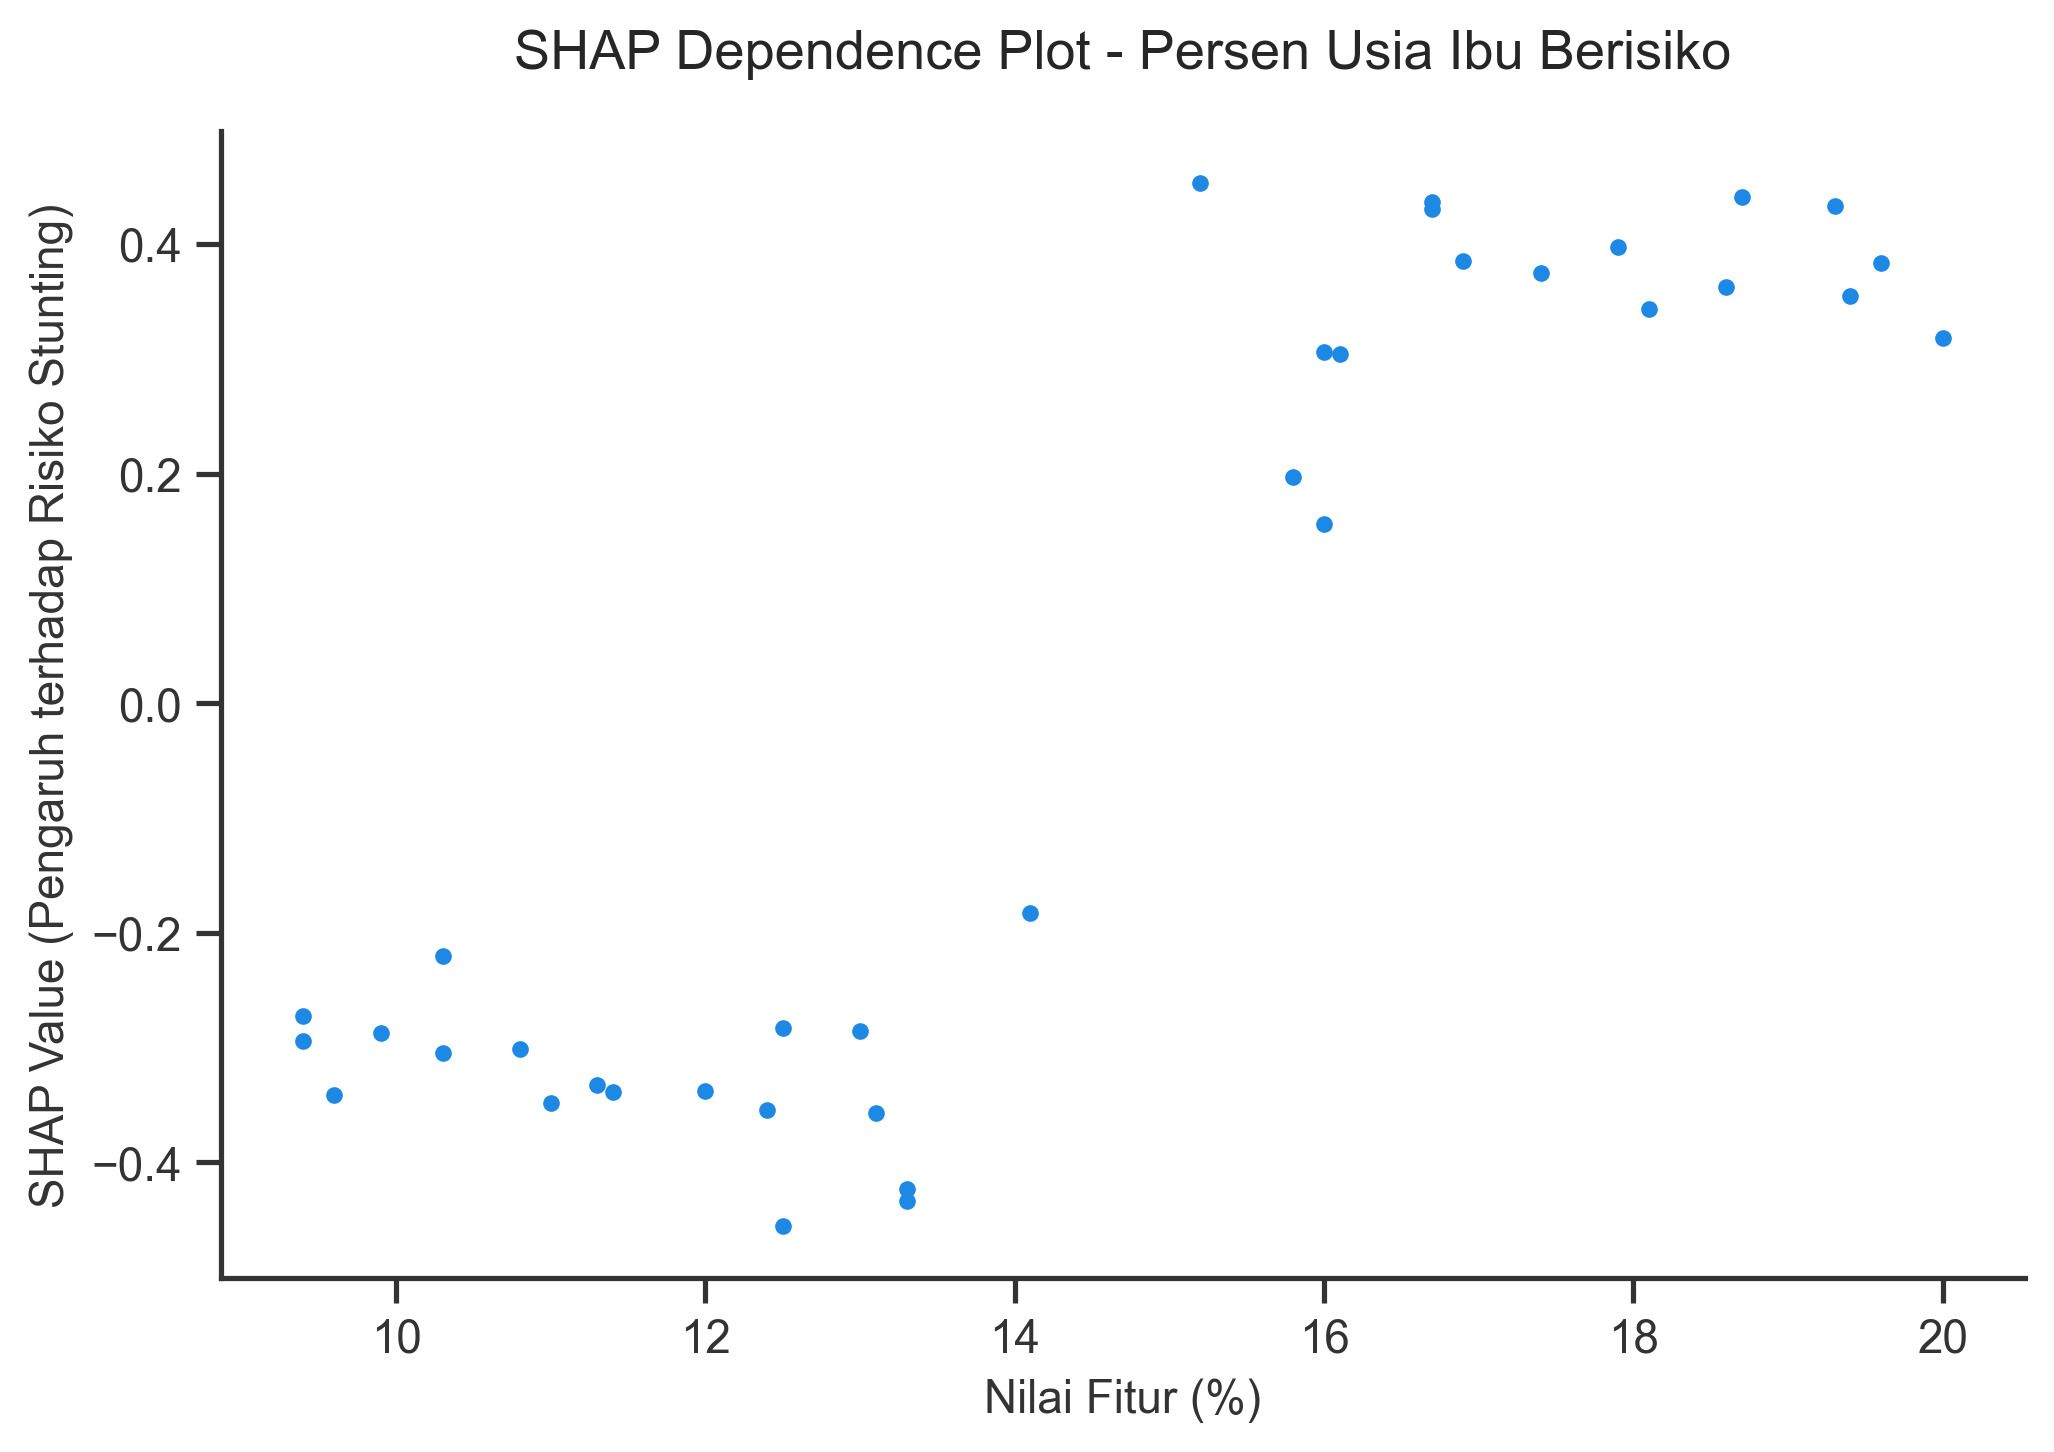
\includegraphics[width=0.48\textwidth]{figure/hasil_dependence_plot/dependence_persen_usia_ibu_berisiko.png} \\ \vspace{0.2cm}
    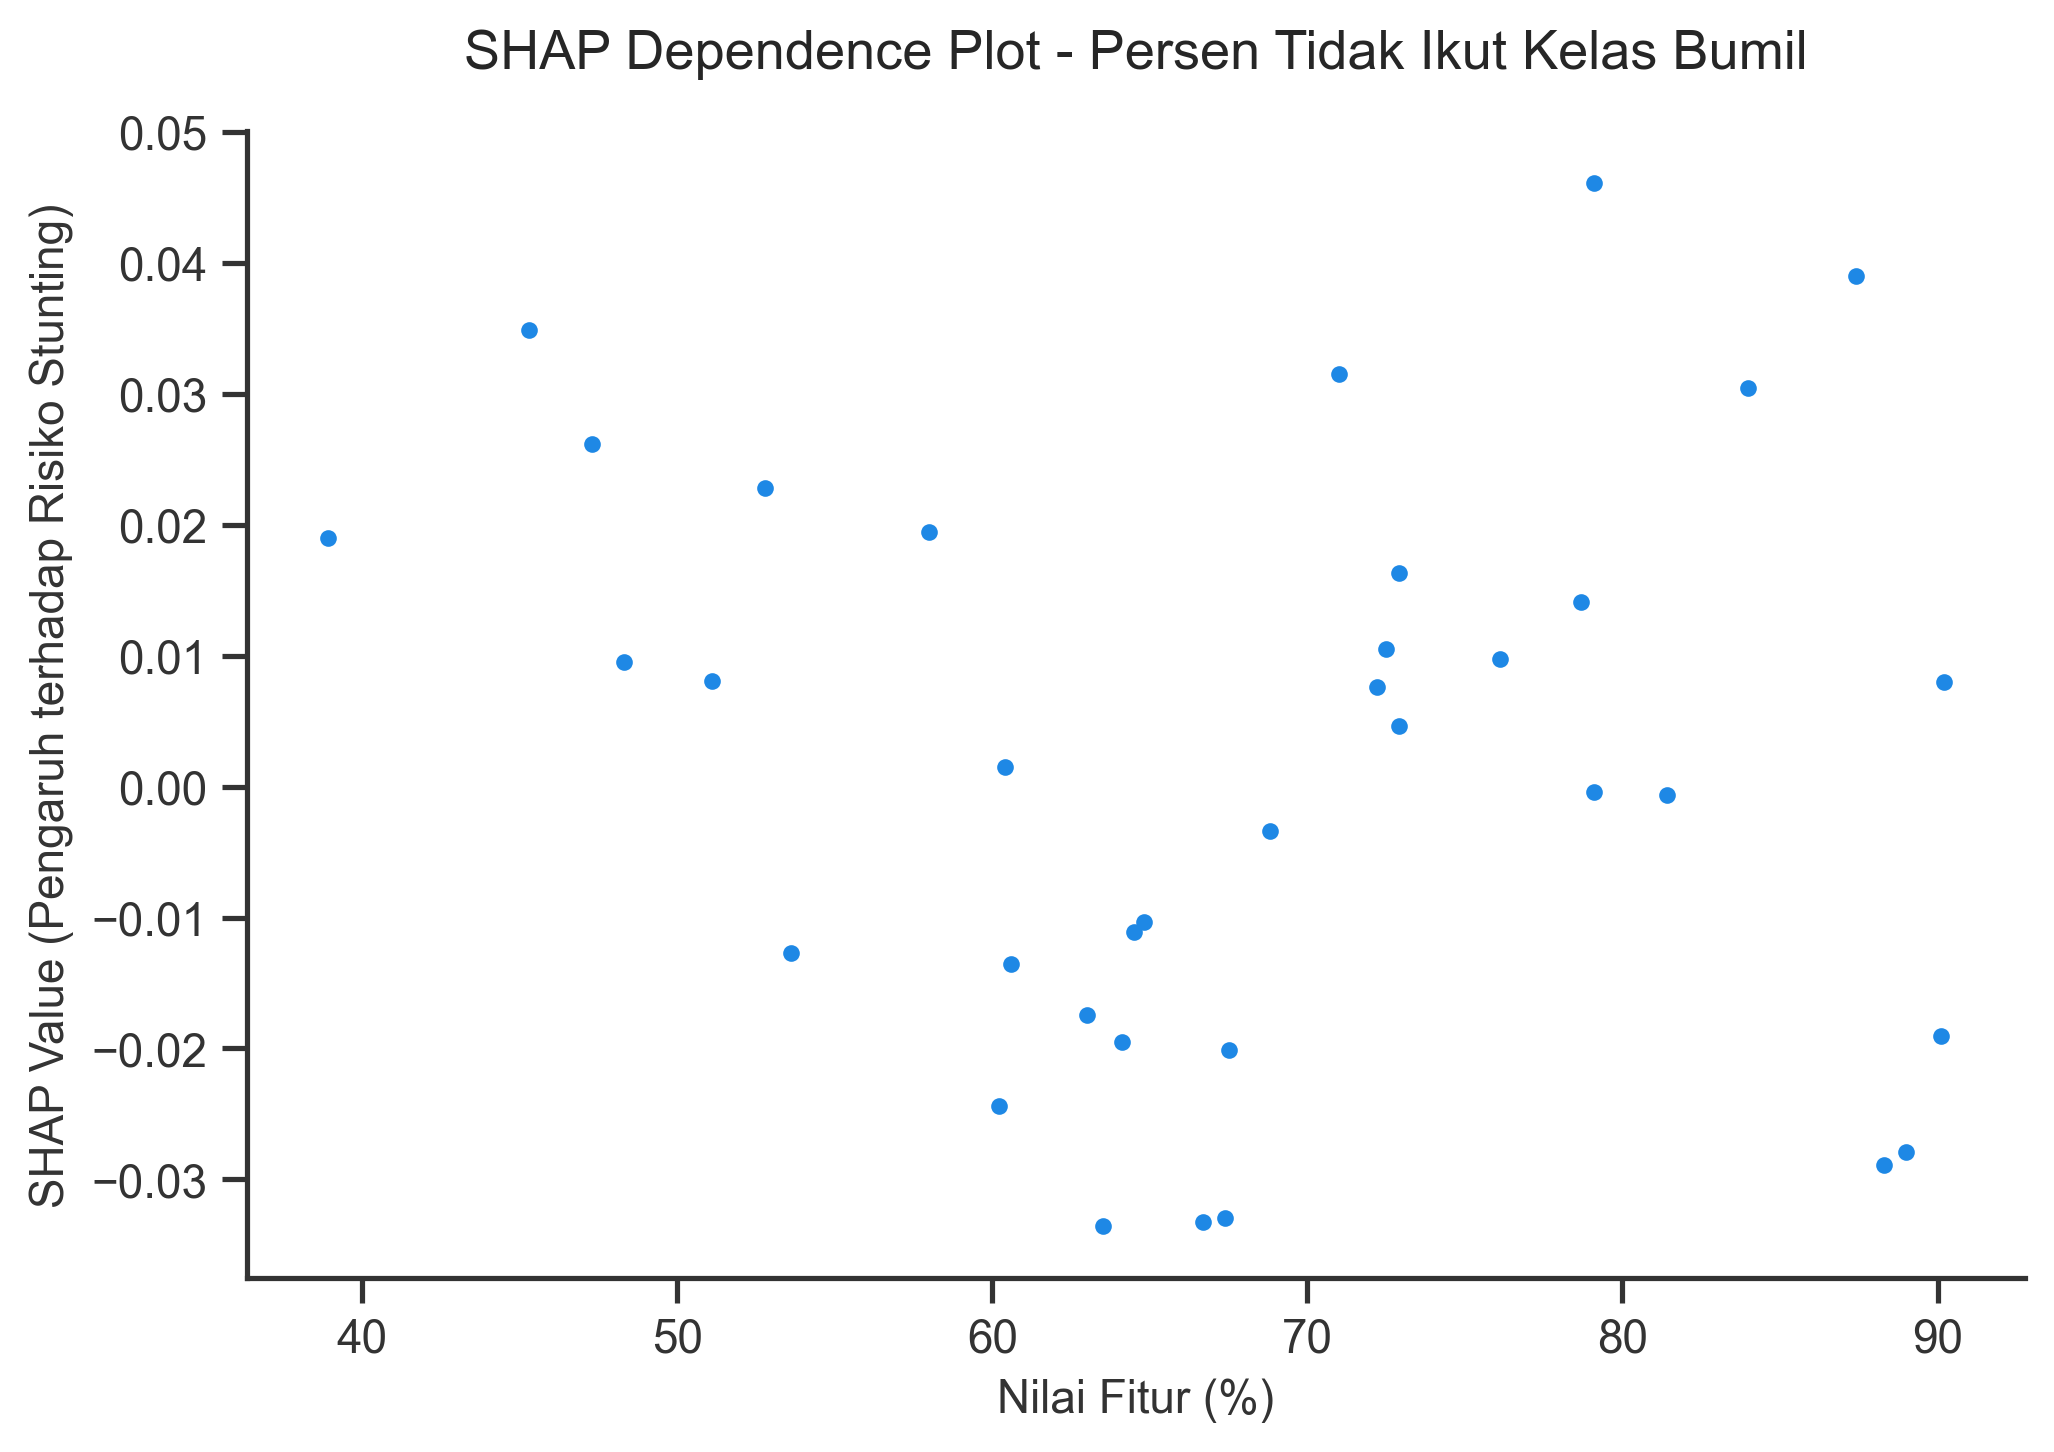
\includegraphics[width=0.48\textwidth]{figure/hasil_dependence_plot/dependence_persen_tidak_ikut_kelas_bumil.png} \hfill
    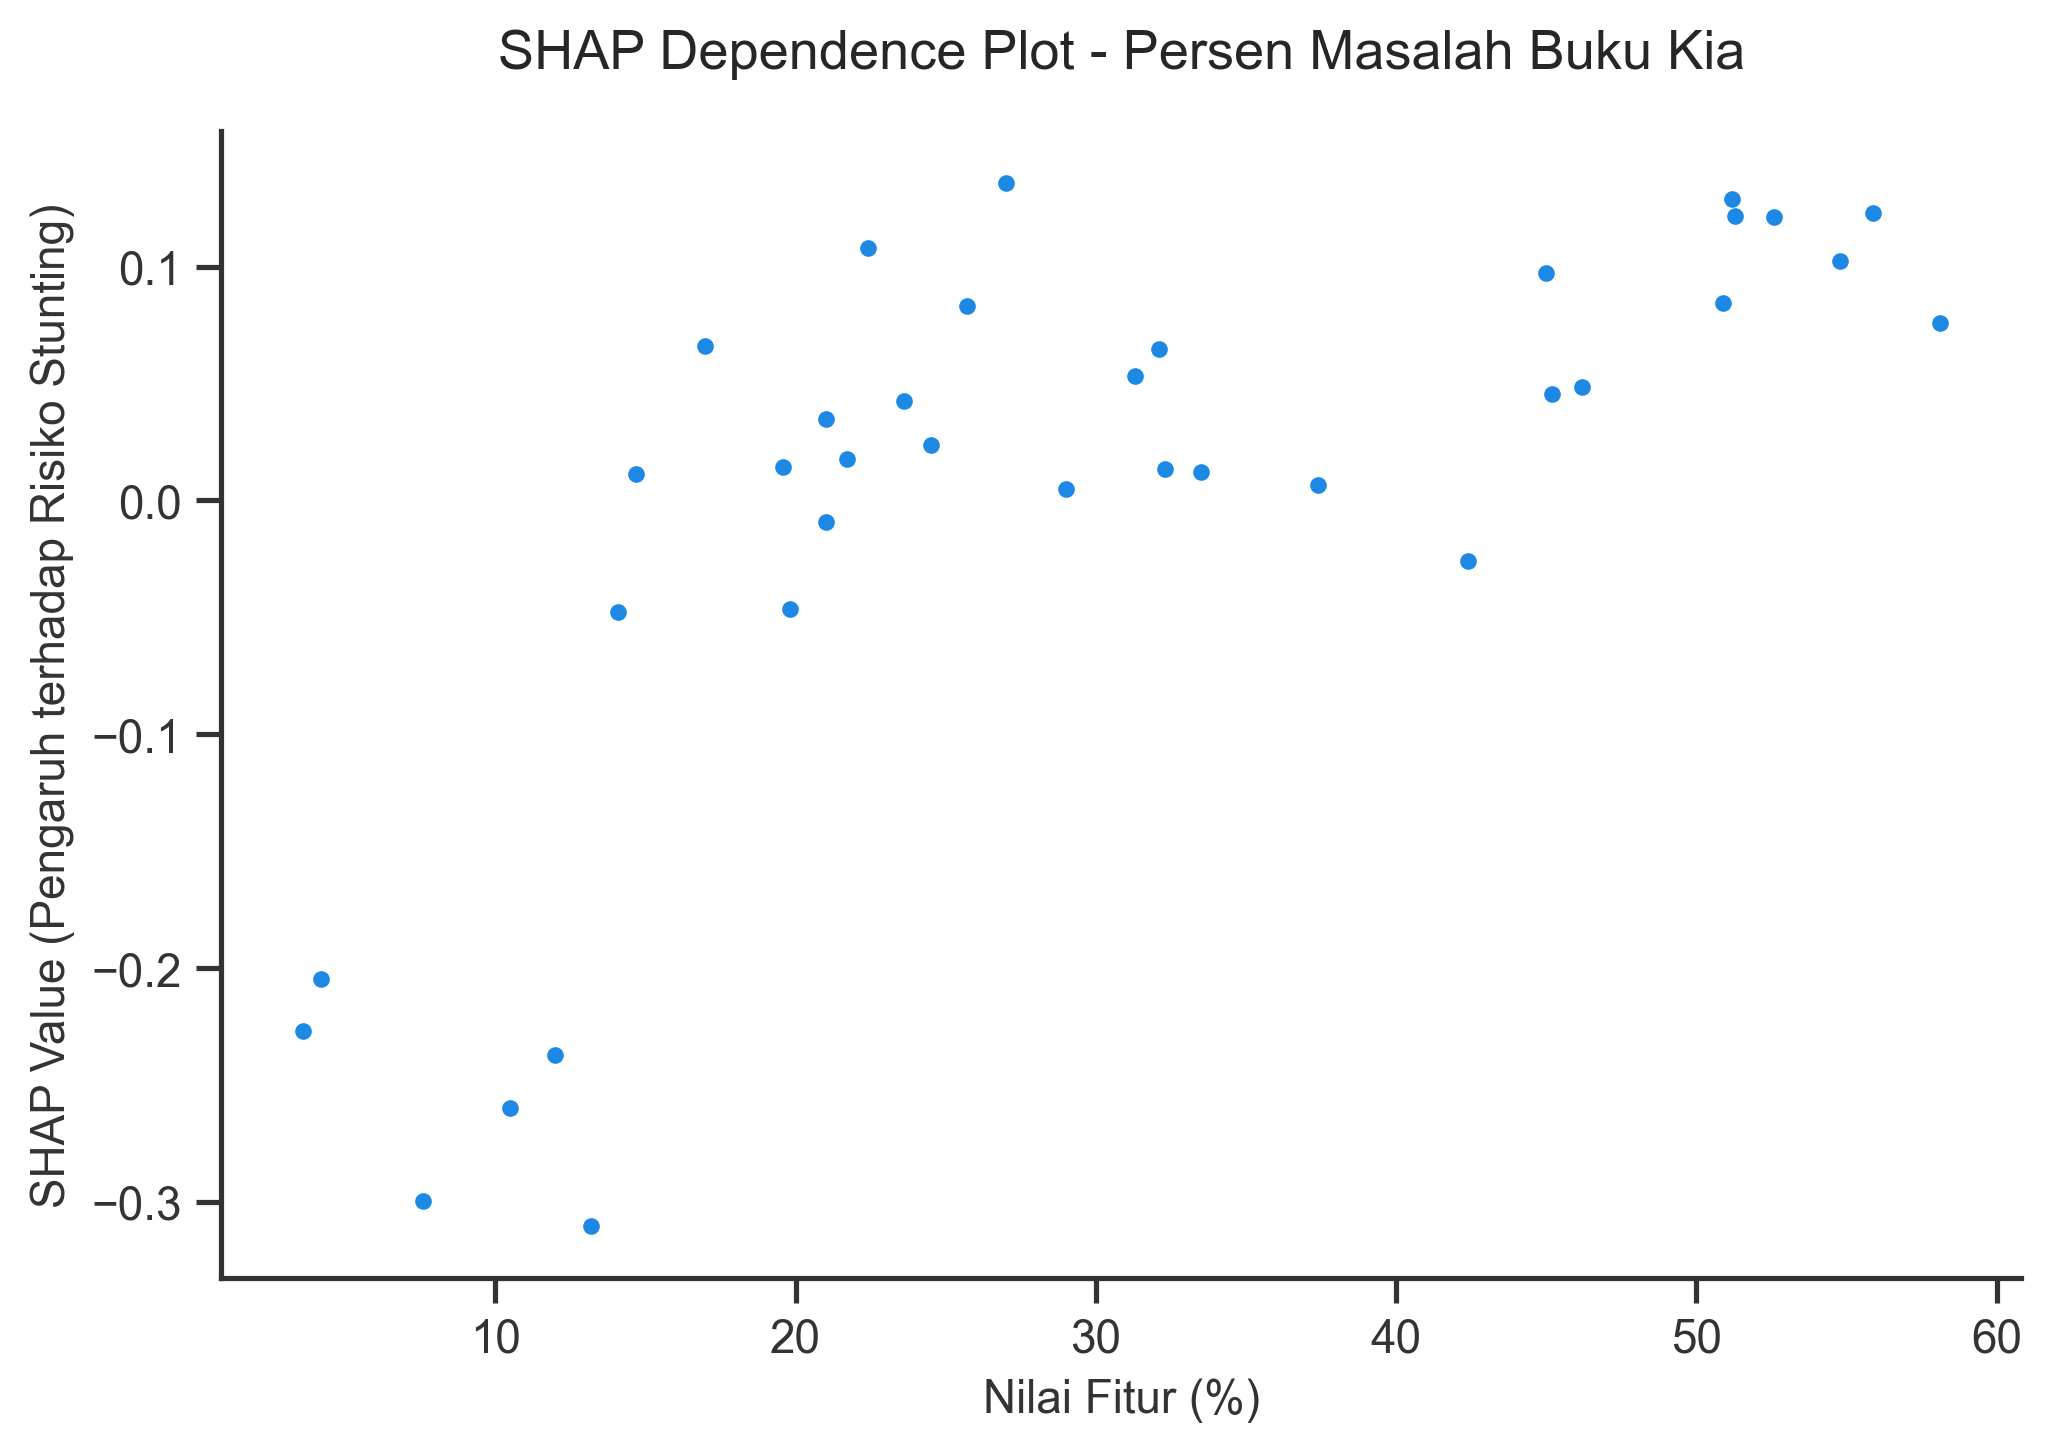
\includegraphics[width=0.48\textwidth]{figure/hasil_dependence_plot/dependence_persen_masalah_buku_kia.png} \\ \vspace{0.2cm}
    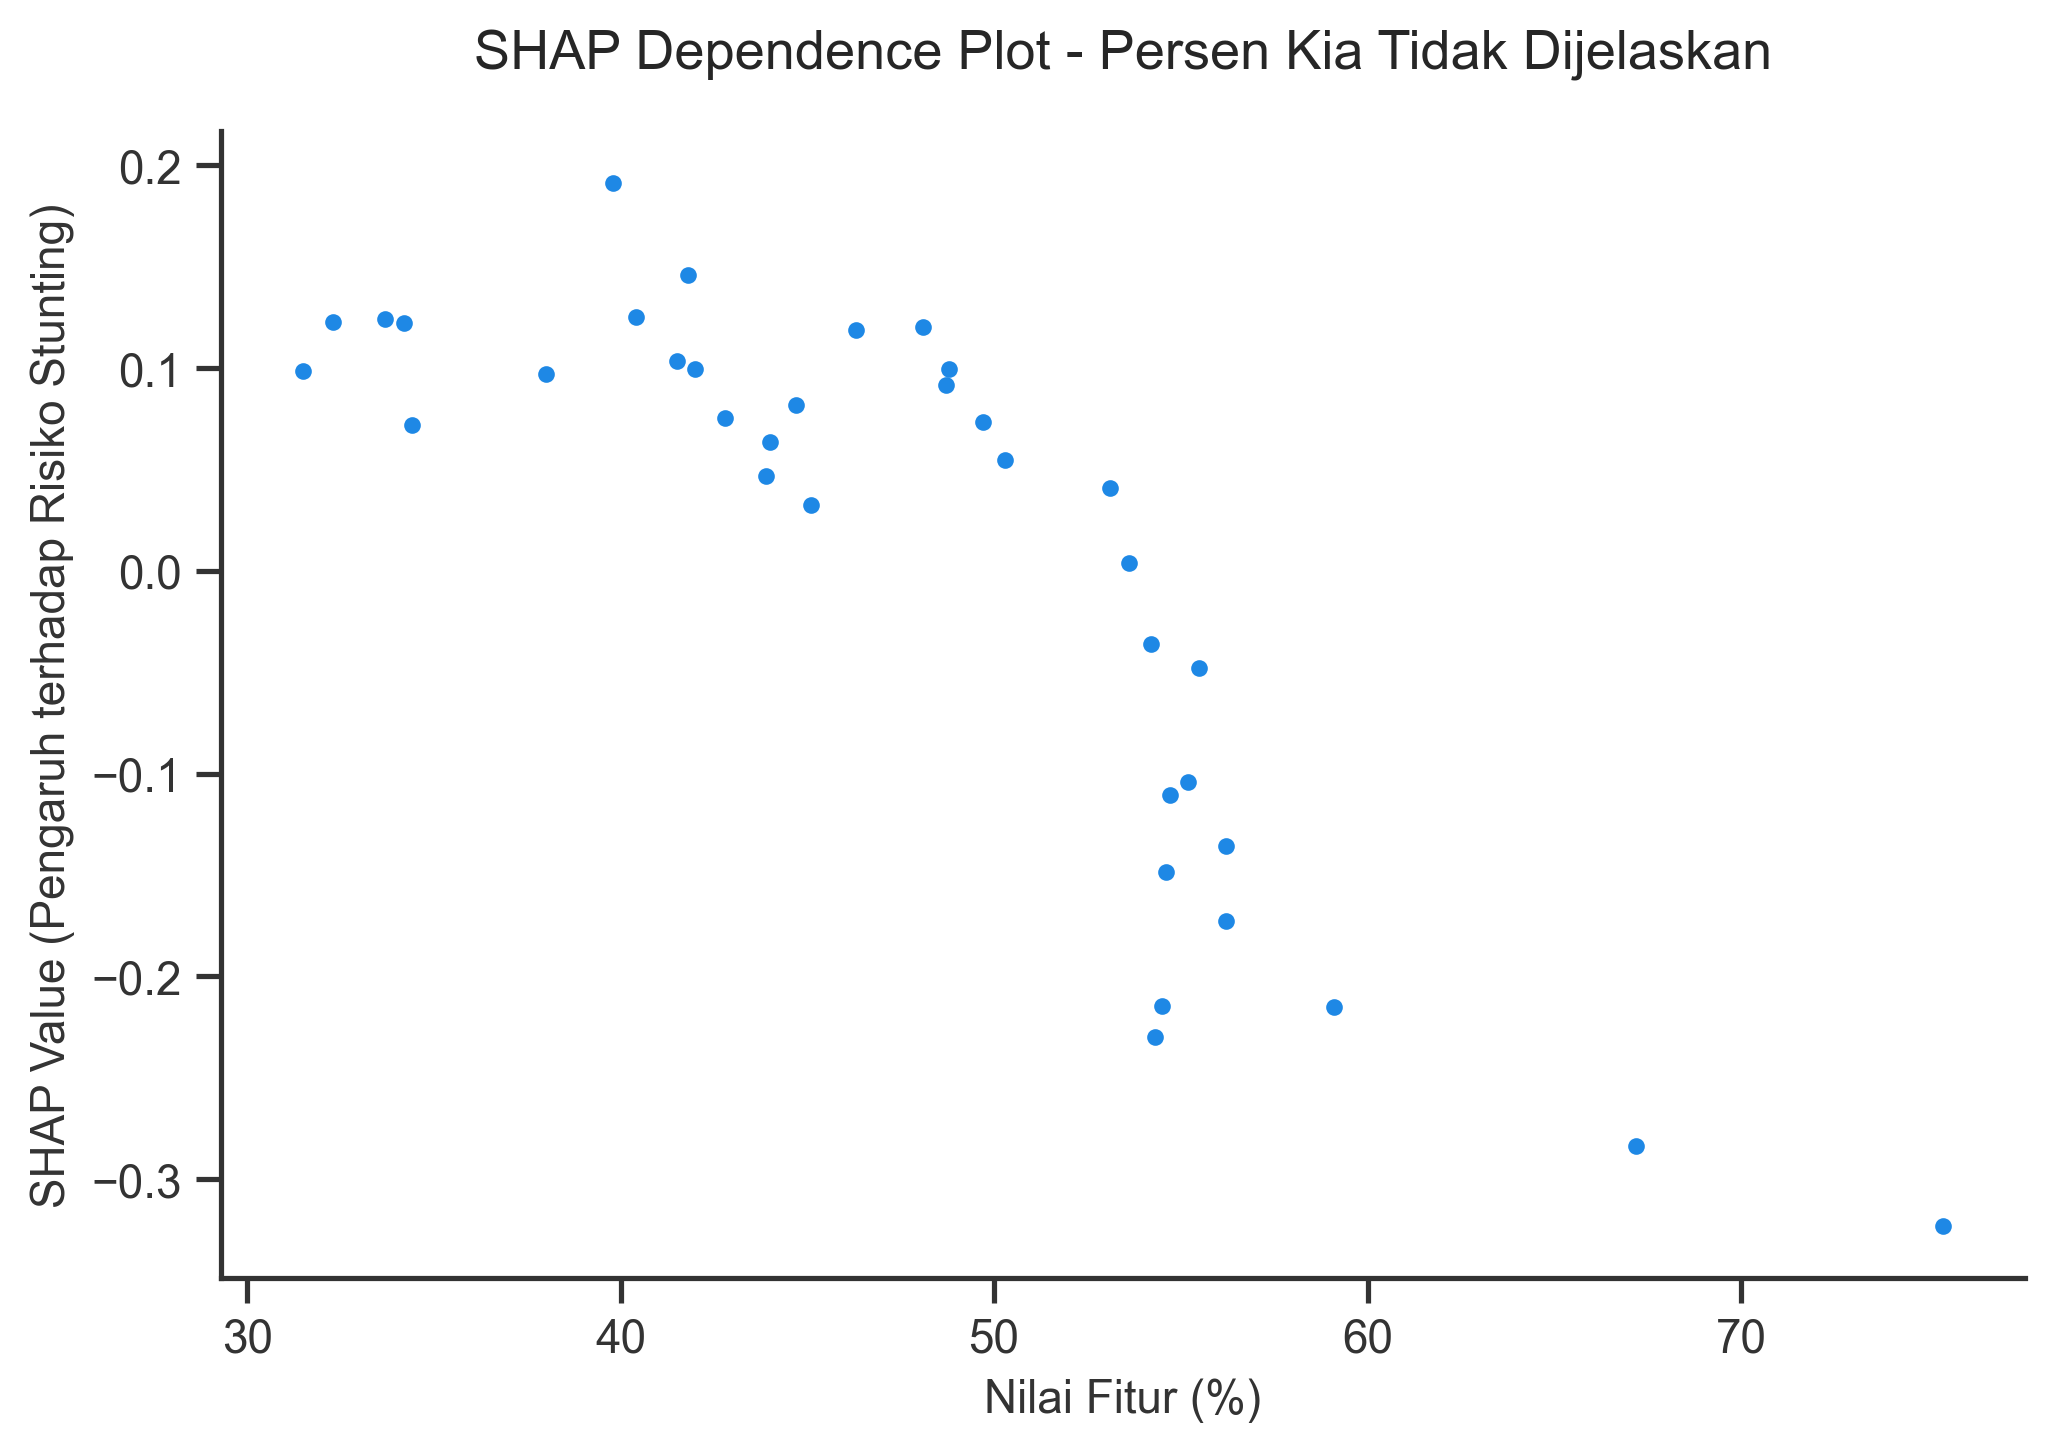
\includegraphics[width=0.48\textwidth]{figure/hasil_dependence_plot/dependence_persen_kia_tidak_dijelaskan.png} \hfill
    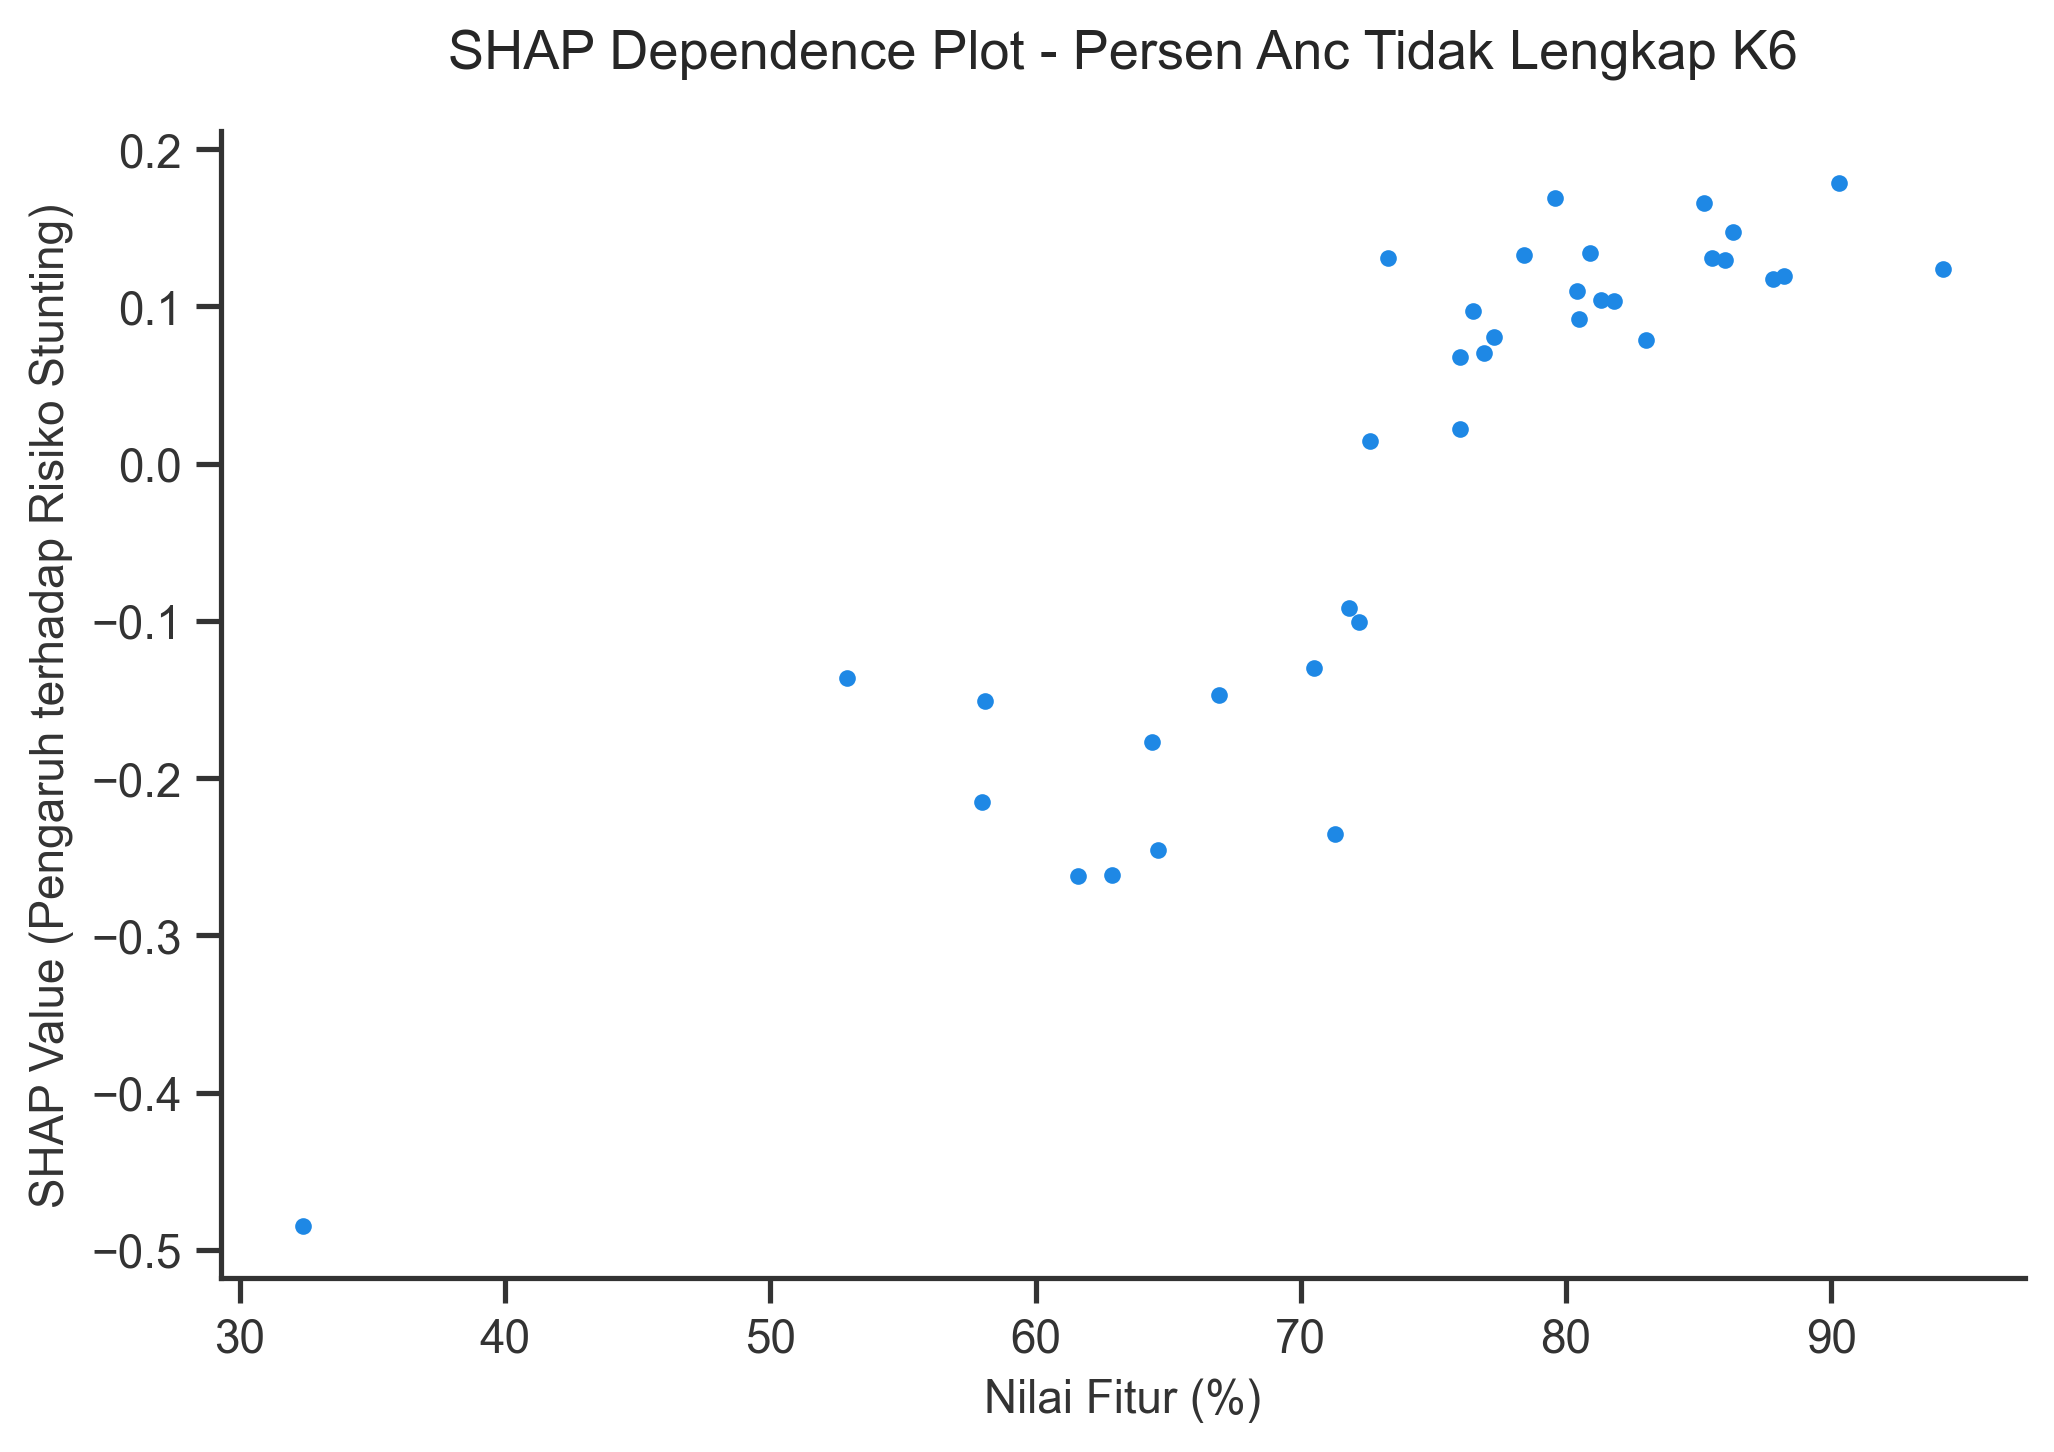
\includegraphics[width=0.48\textwidth]{figure/hasil_dependence_plot/dependence_persen_anc_tidak_lengkap_k6.png} \\ \vspace{0.2cm}
    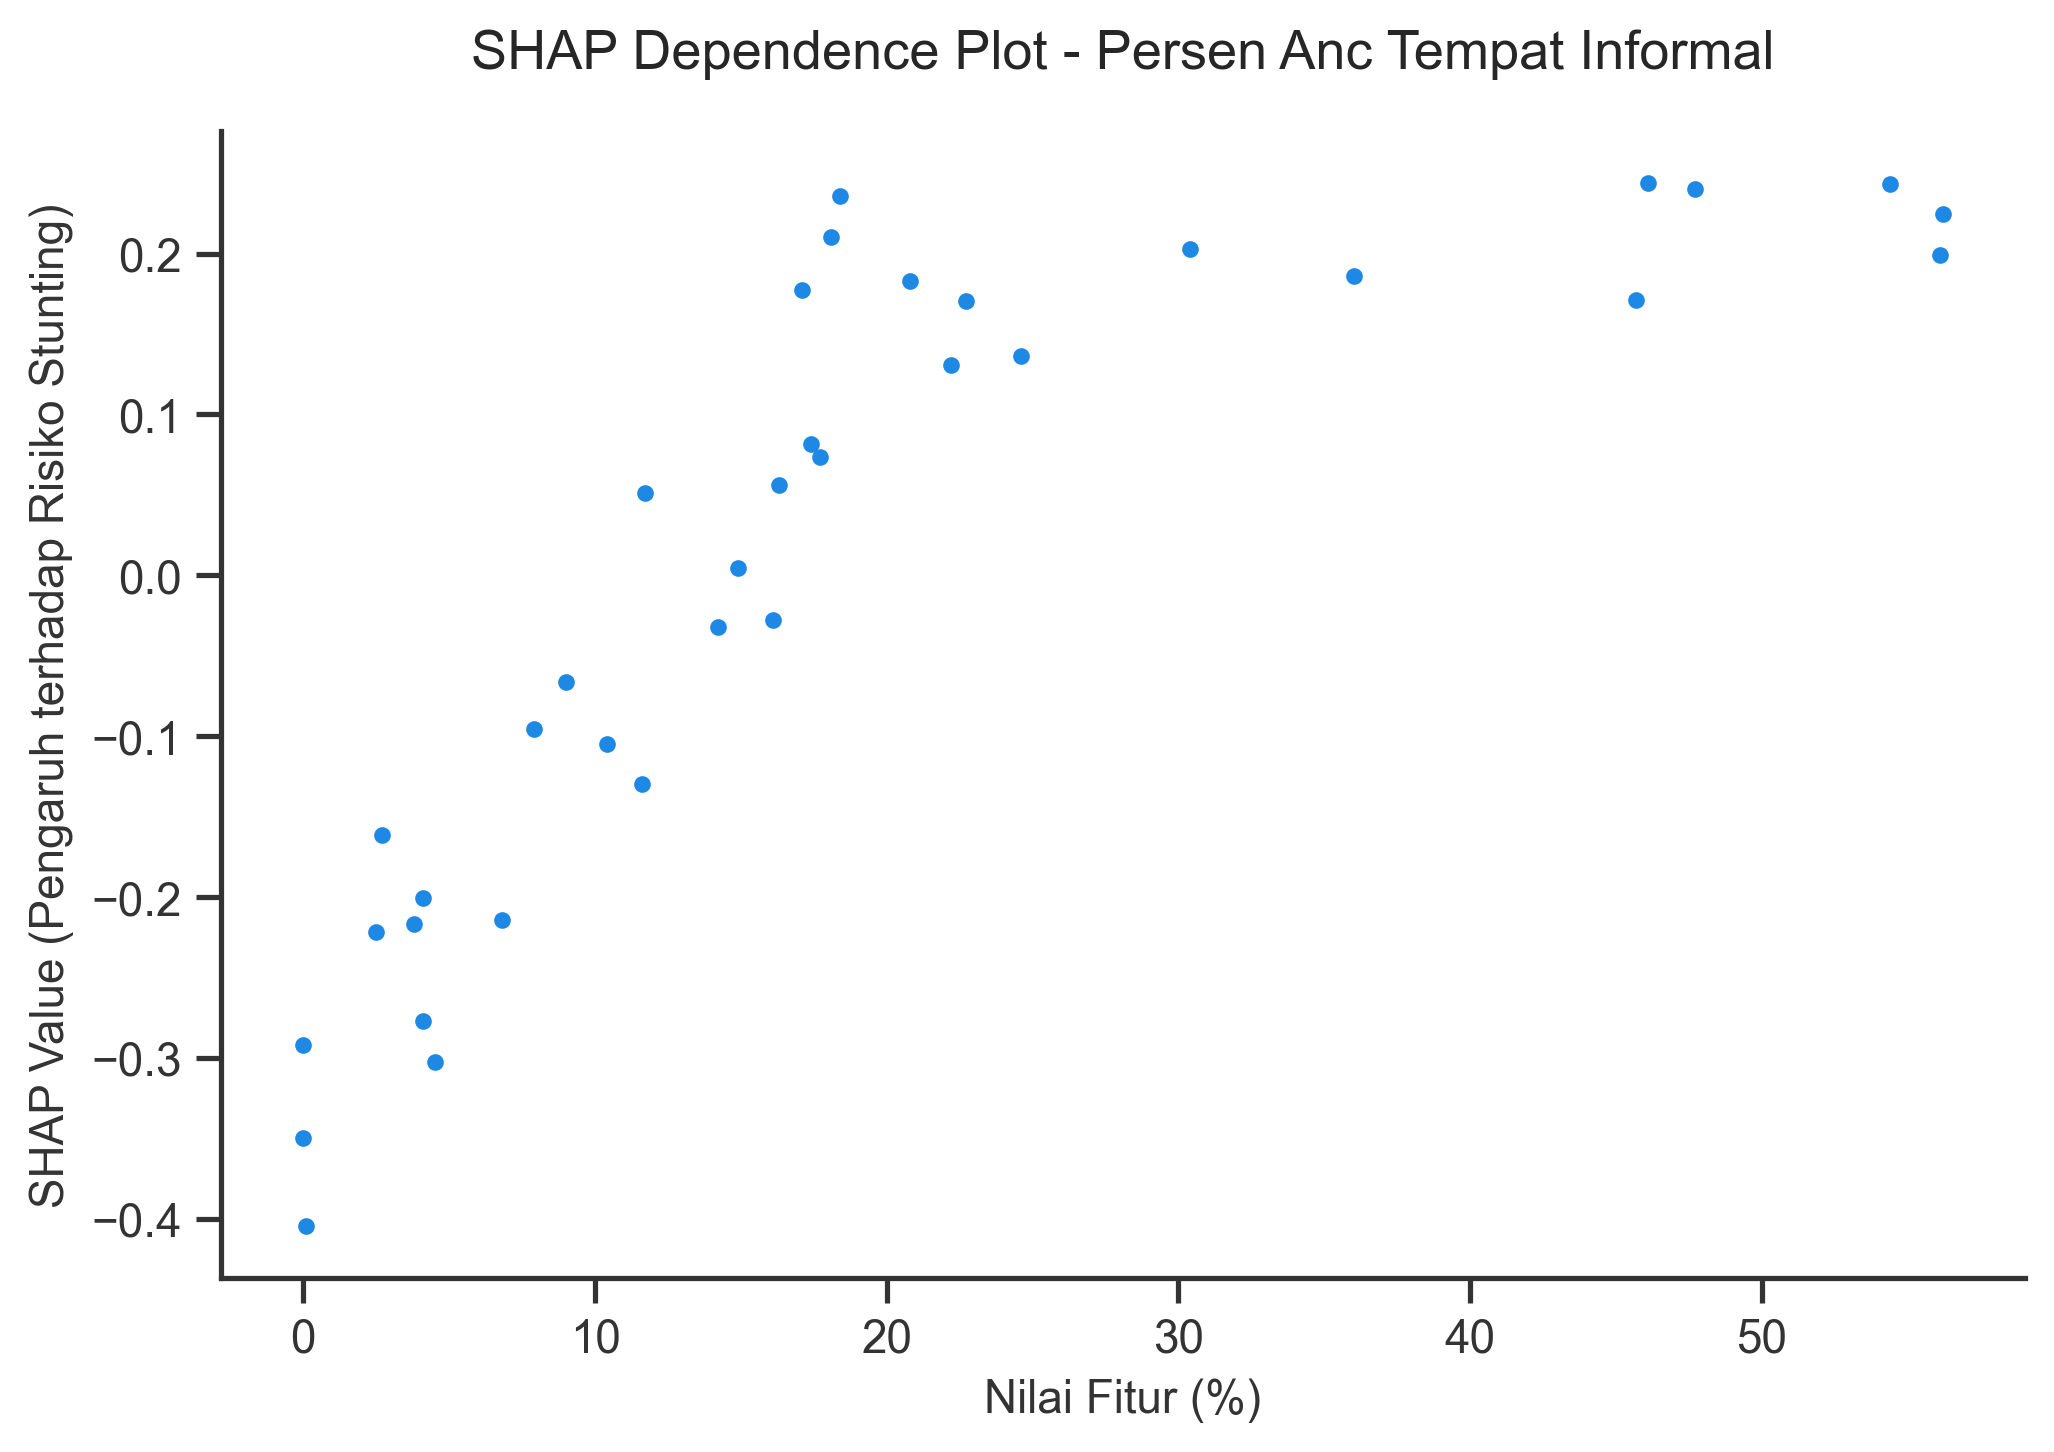
\includegraphics[width=0.48\textwidth]{figure/hasil_dependence_plot/dependence_persen_anc_tempat_informal.png} \hfill
    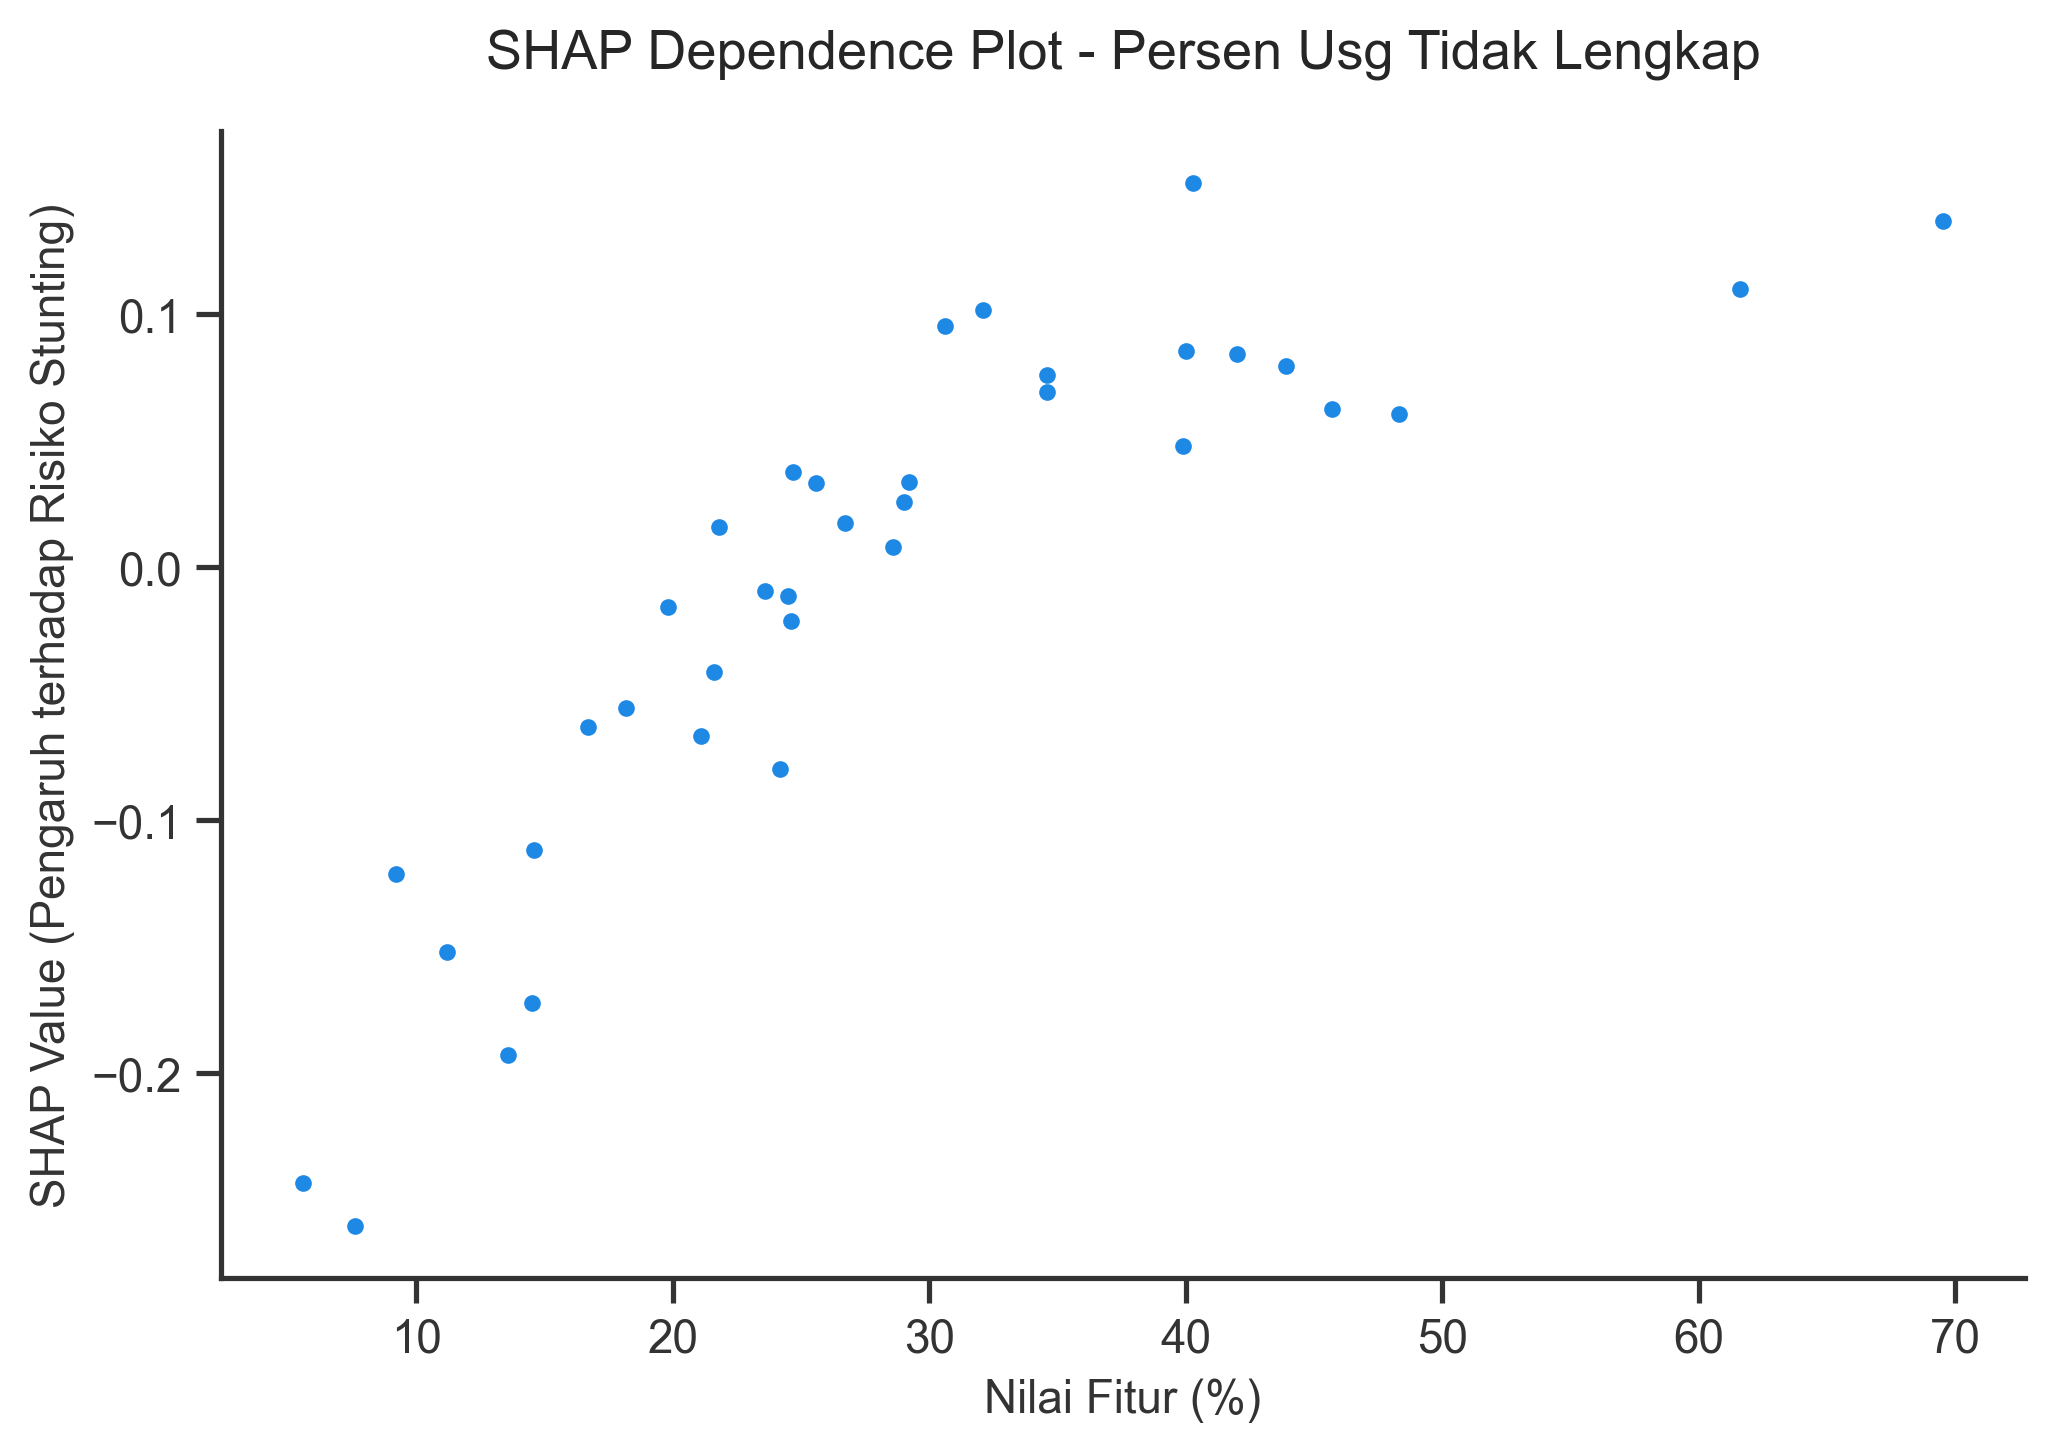
\includegraphics[width=0.48\textwidth]{figure/hasil_dependence_plot/dependence_persen_usg_tidak_lengkap.png}
\end{figure}

\newpage
\begin{figure}[H]
    \centering
    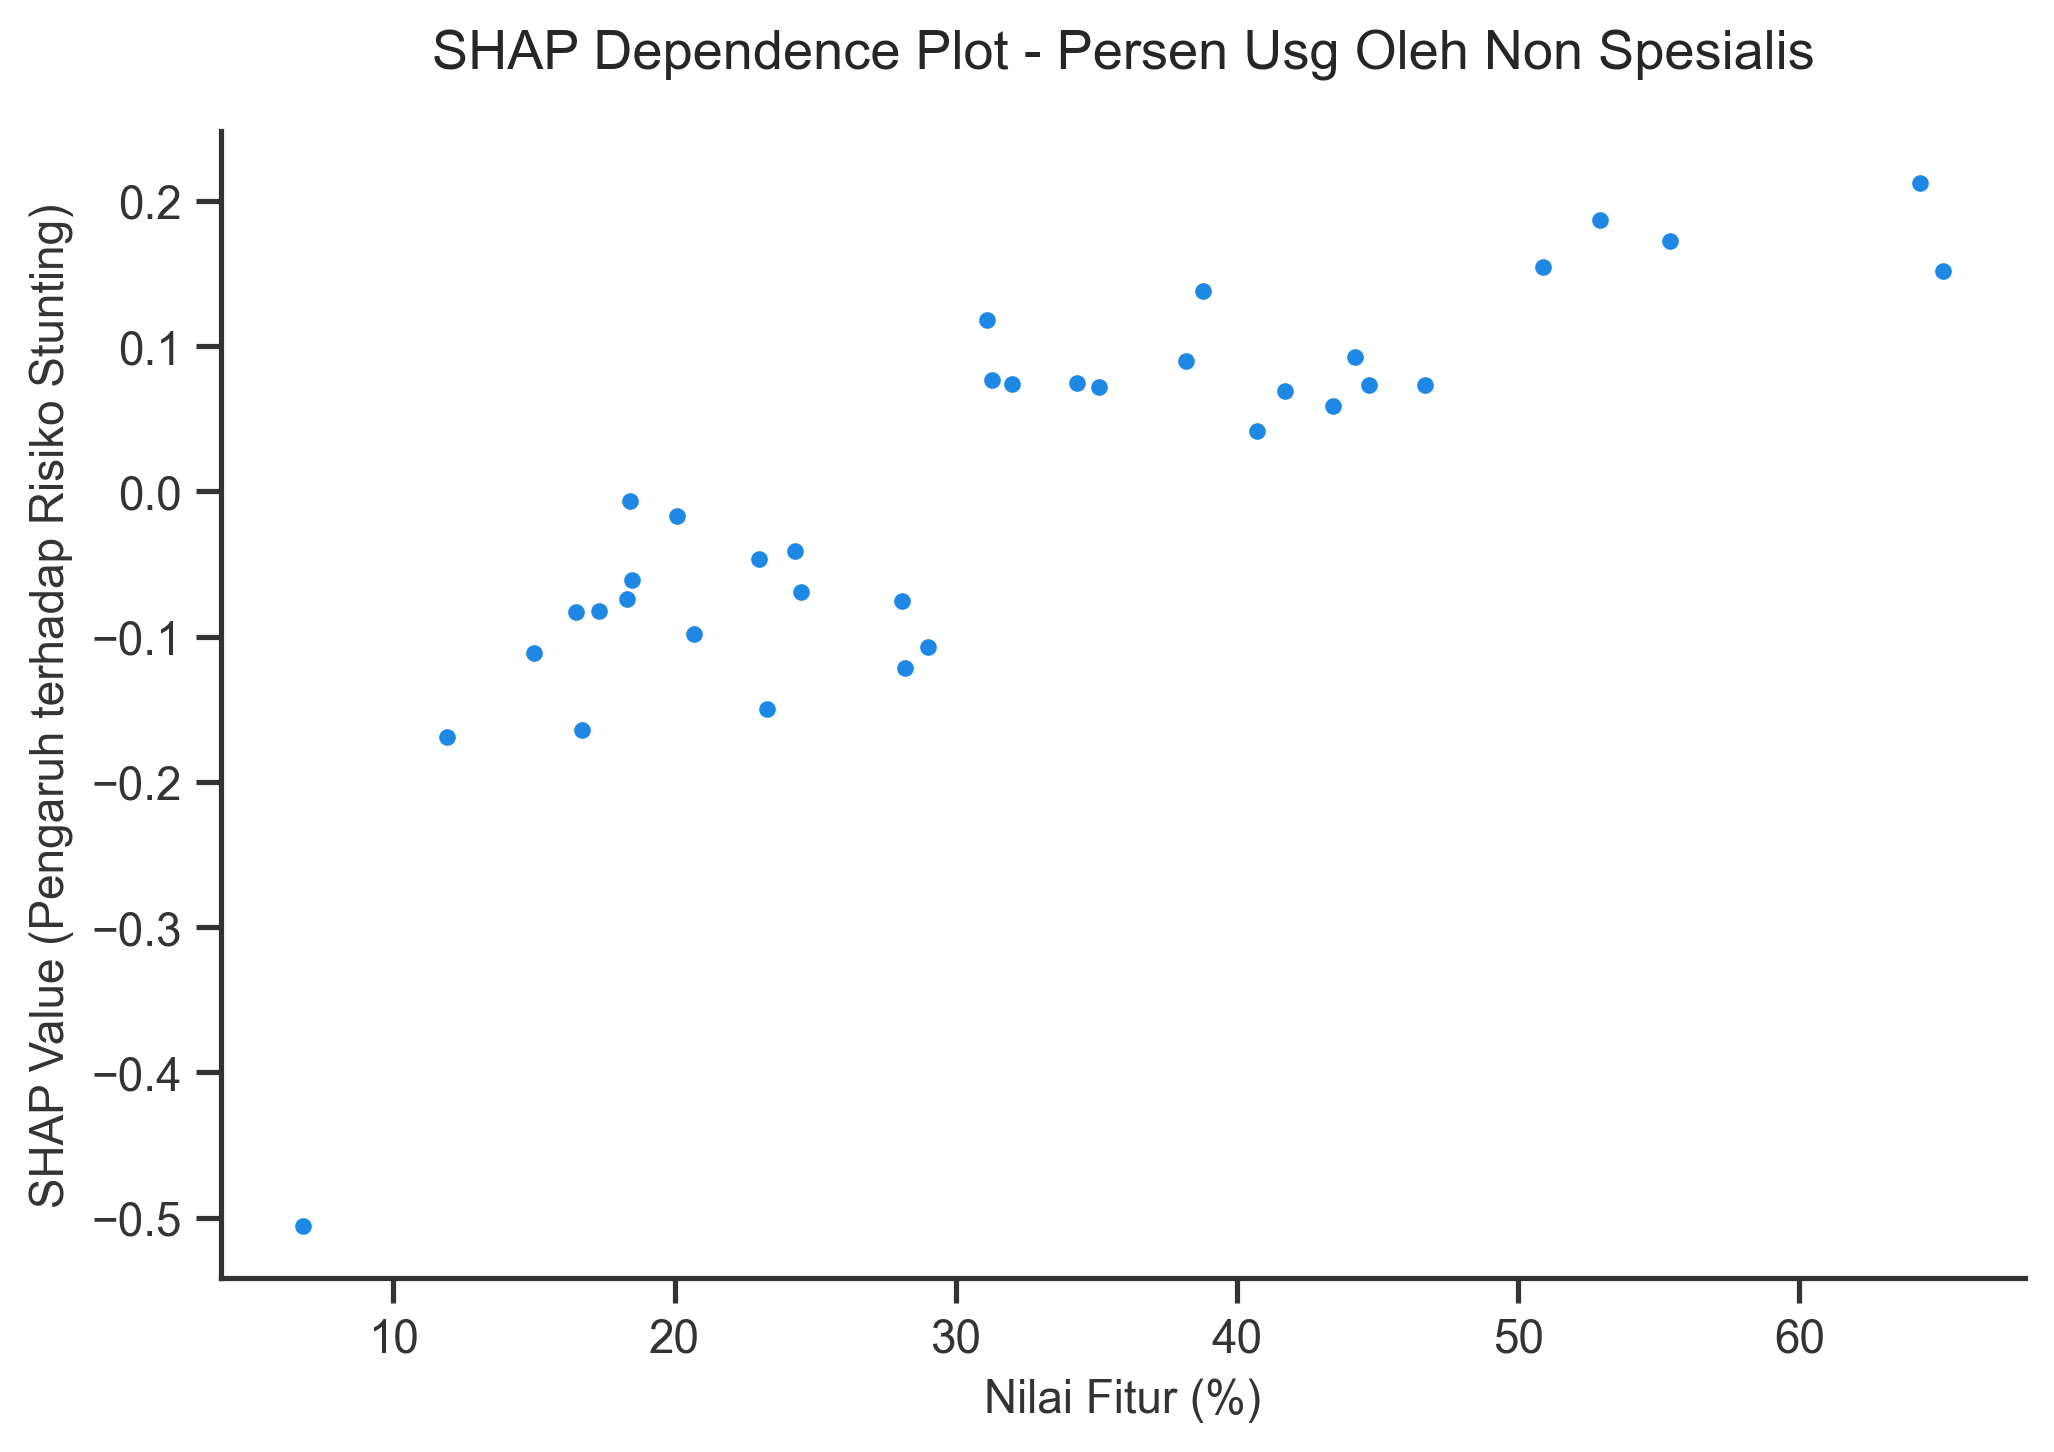
\includegraphics[width=0.48\textwidth]{figure/hasil_dependence_plot/dependence_persen_usg_oleh_non_spesialis.png} \hfill
    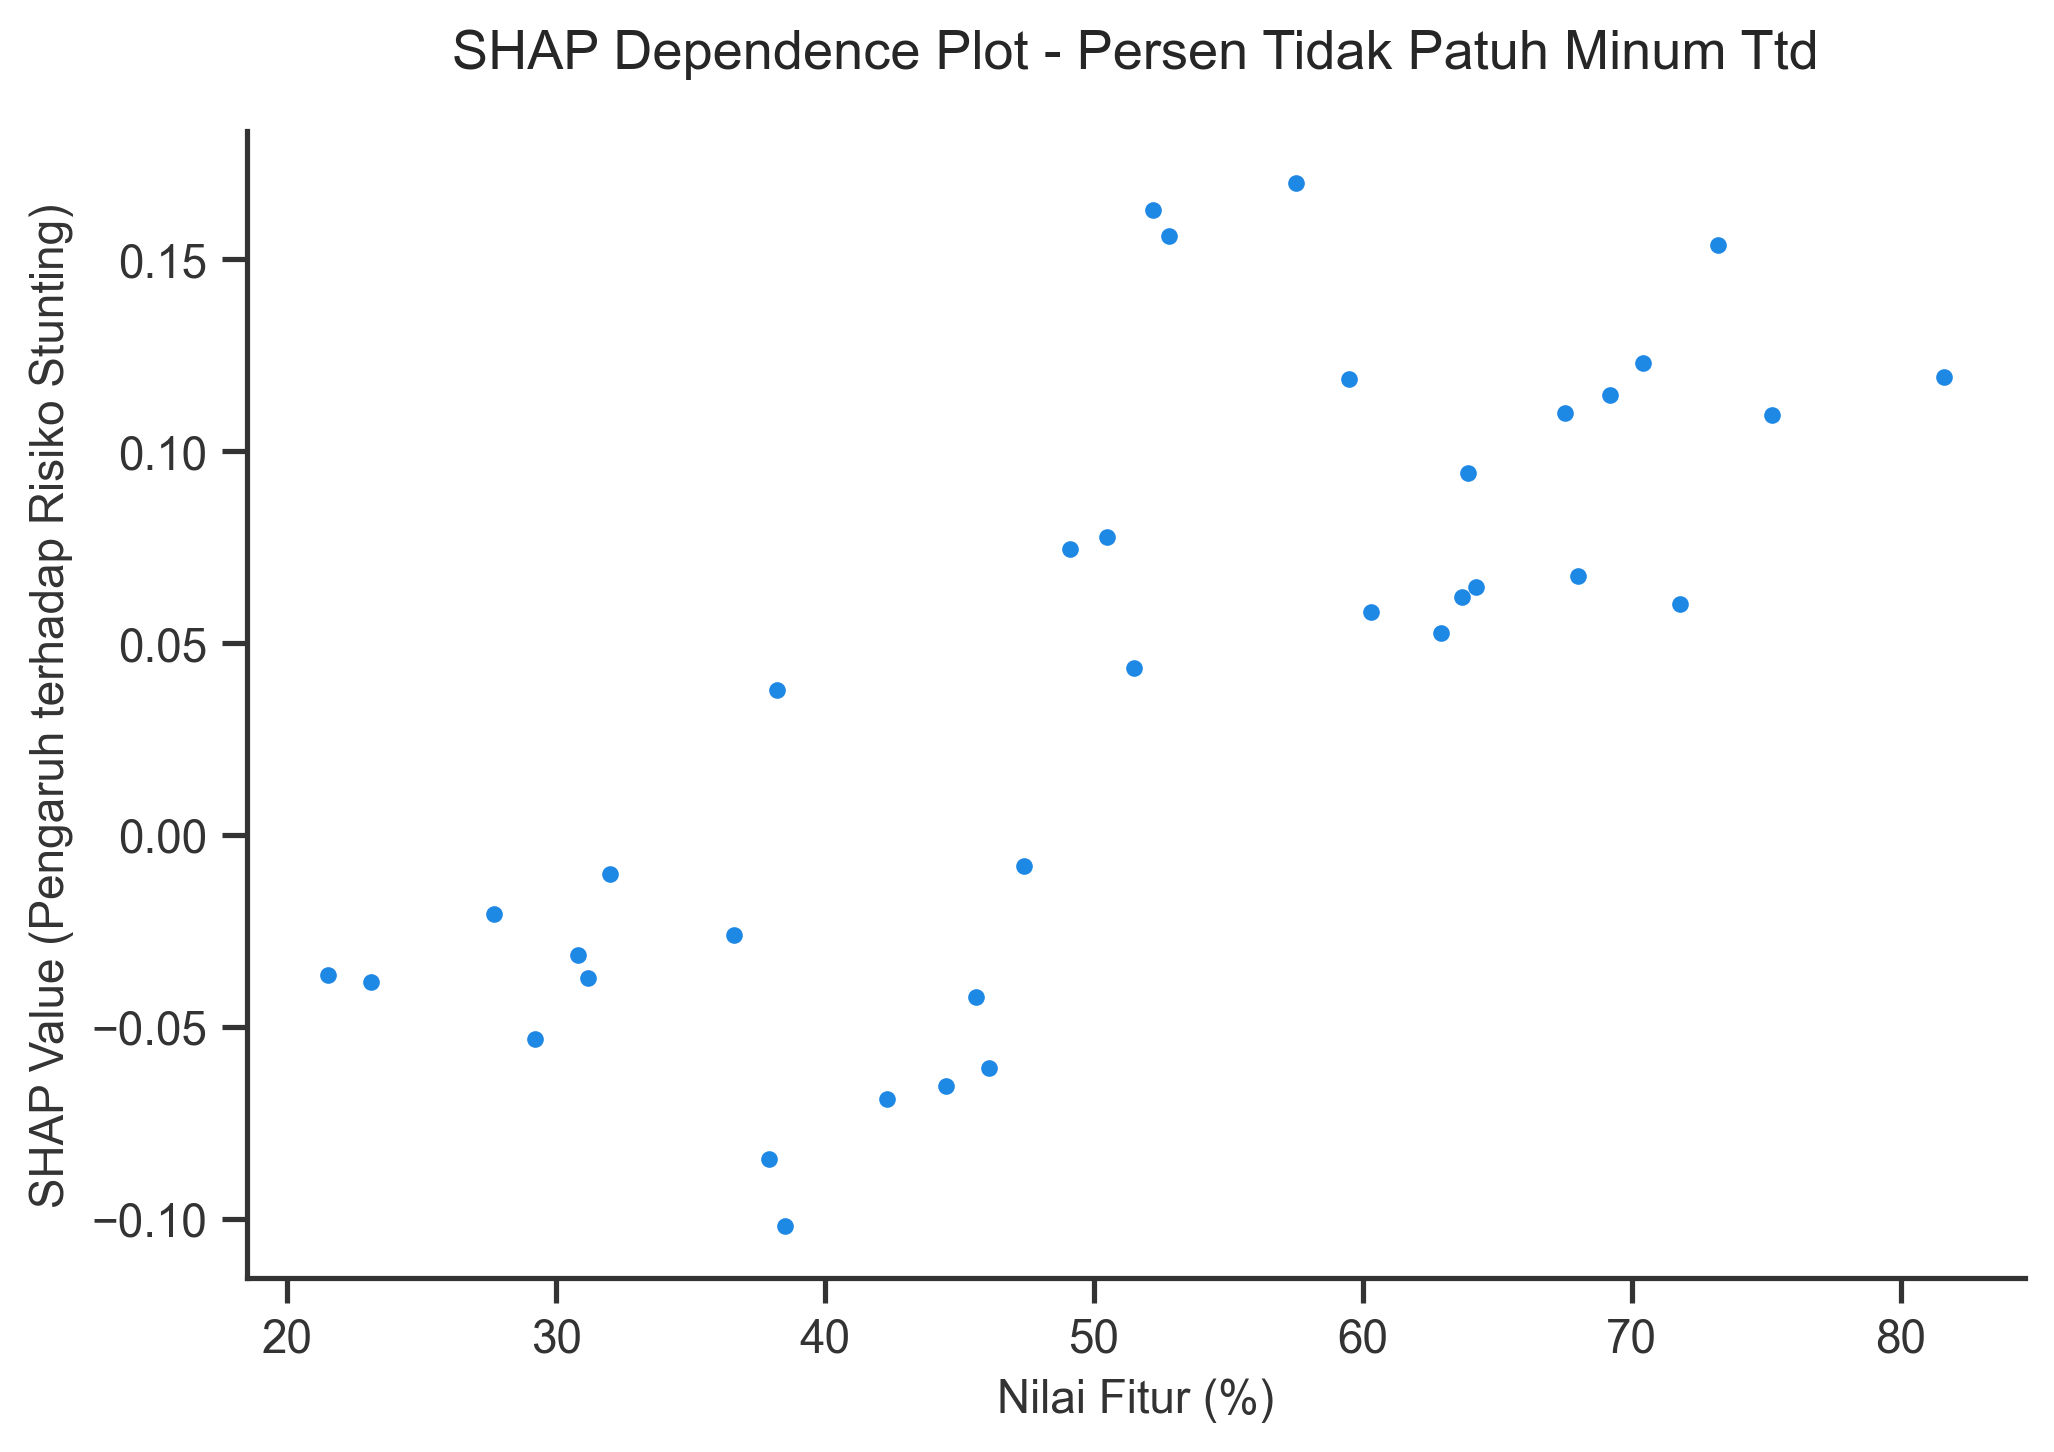
\includegraphics[width=0.48\textwidth]{figure/hasil_dependence_plot/dependence_persen_tidak_patuh_minum_ttd.png} \\ \vspace{0.2cm}
    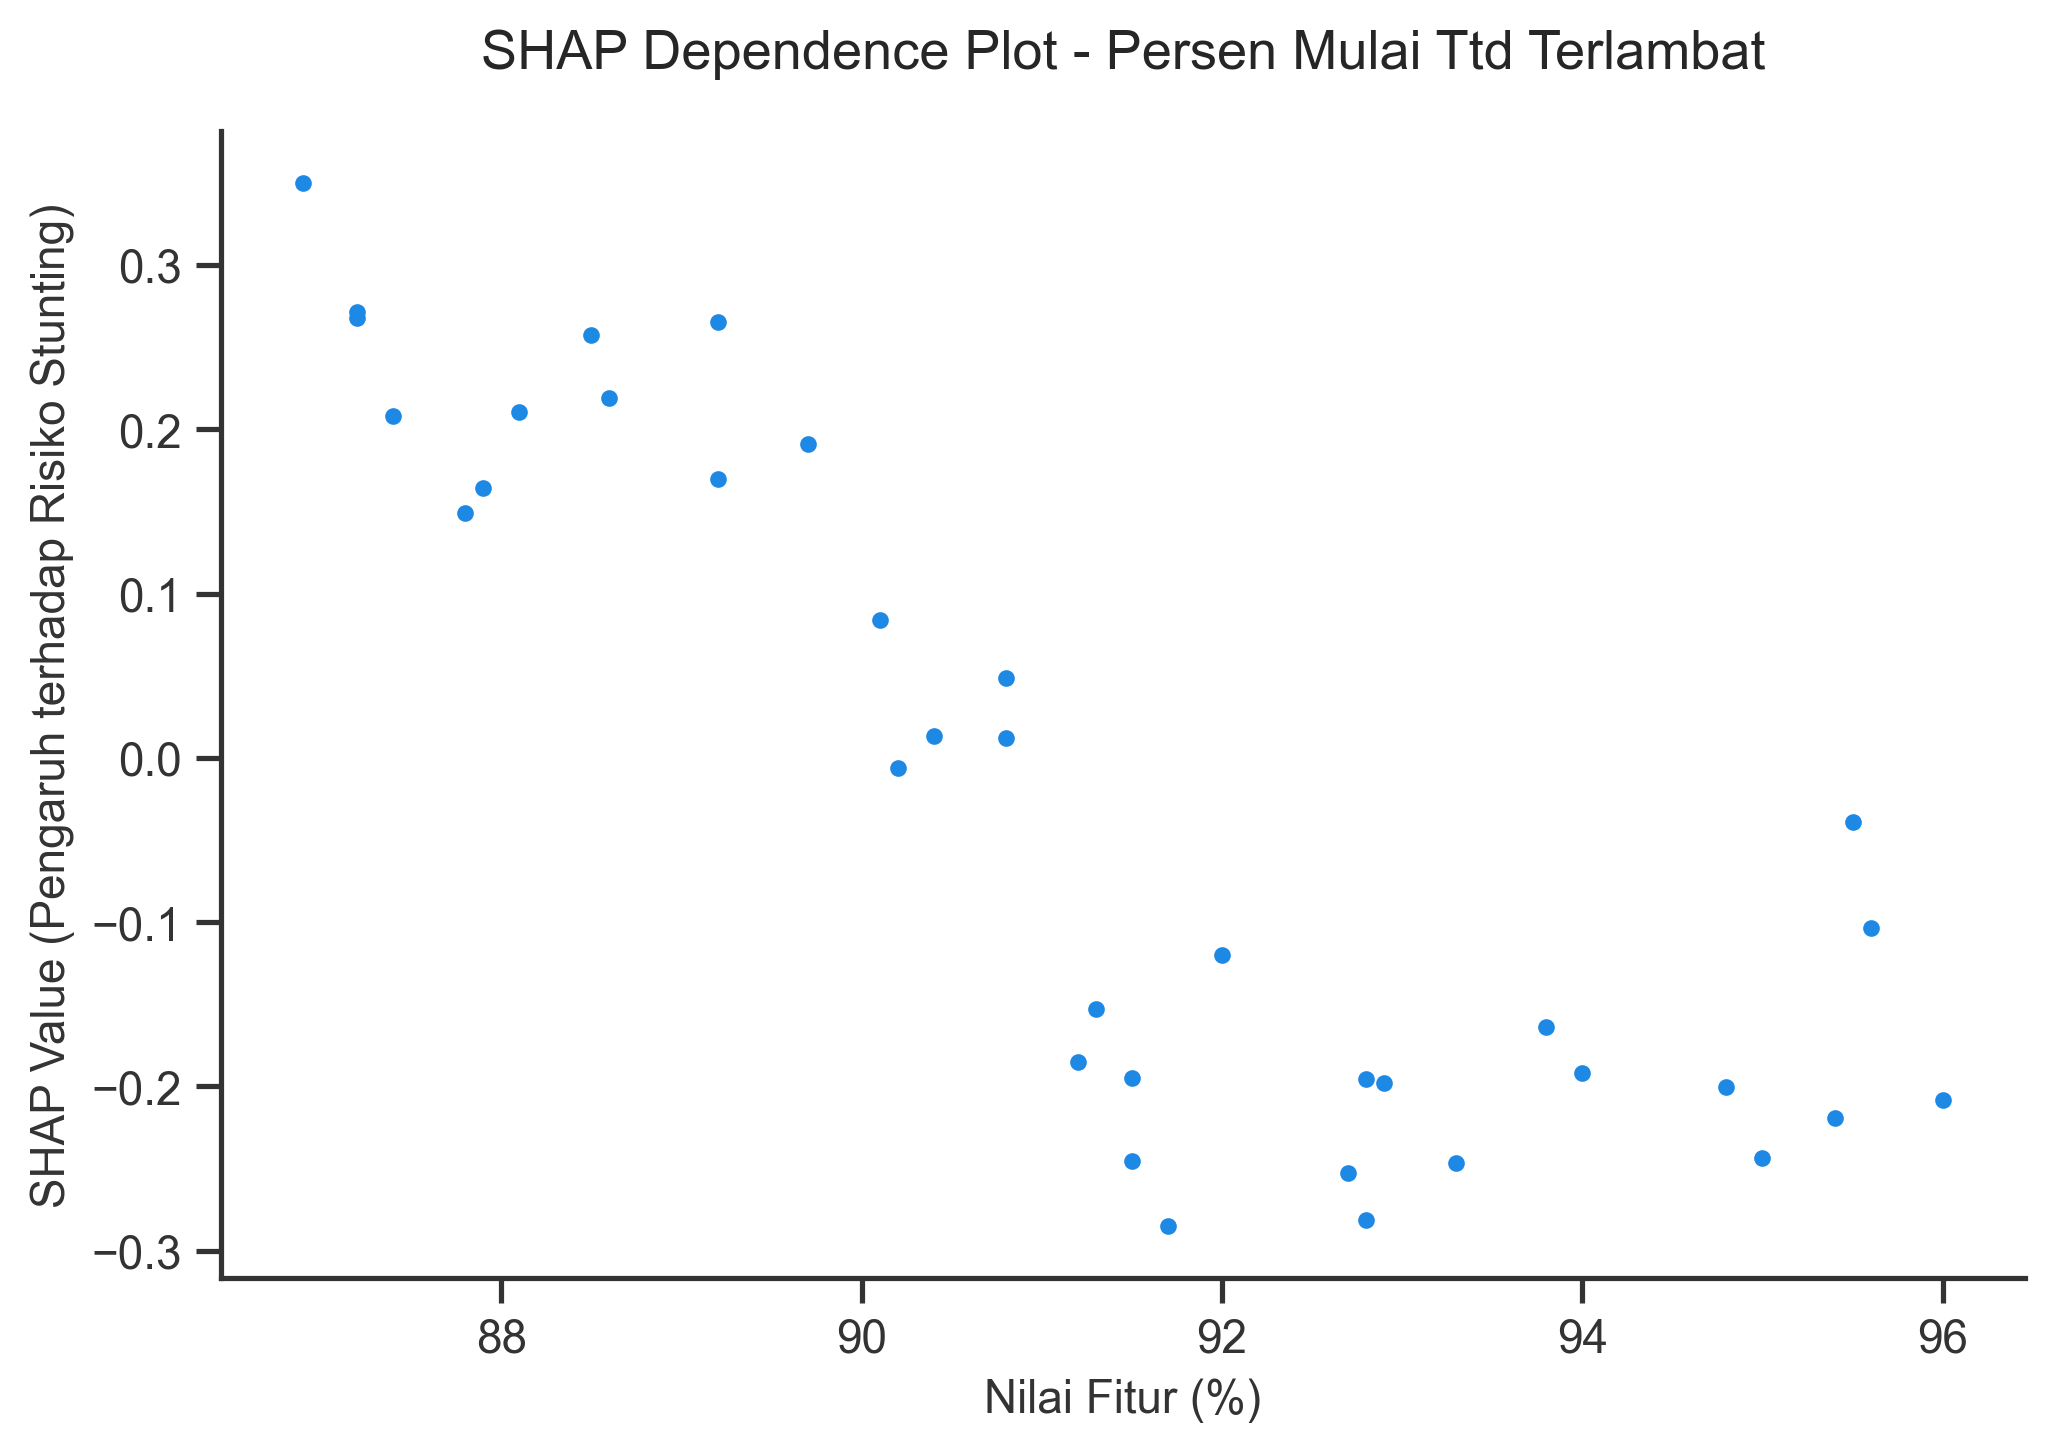
\includegraphics[width=0.48\textwidth]{figure/hasil_dependence_plot/dependence_persen_mulai_ttd_terlambat.png} \hfill
    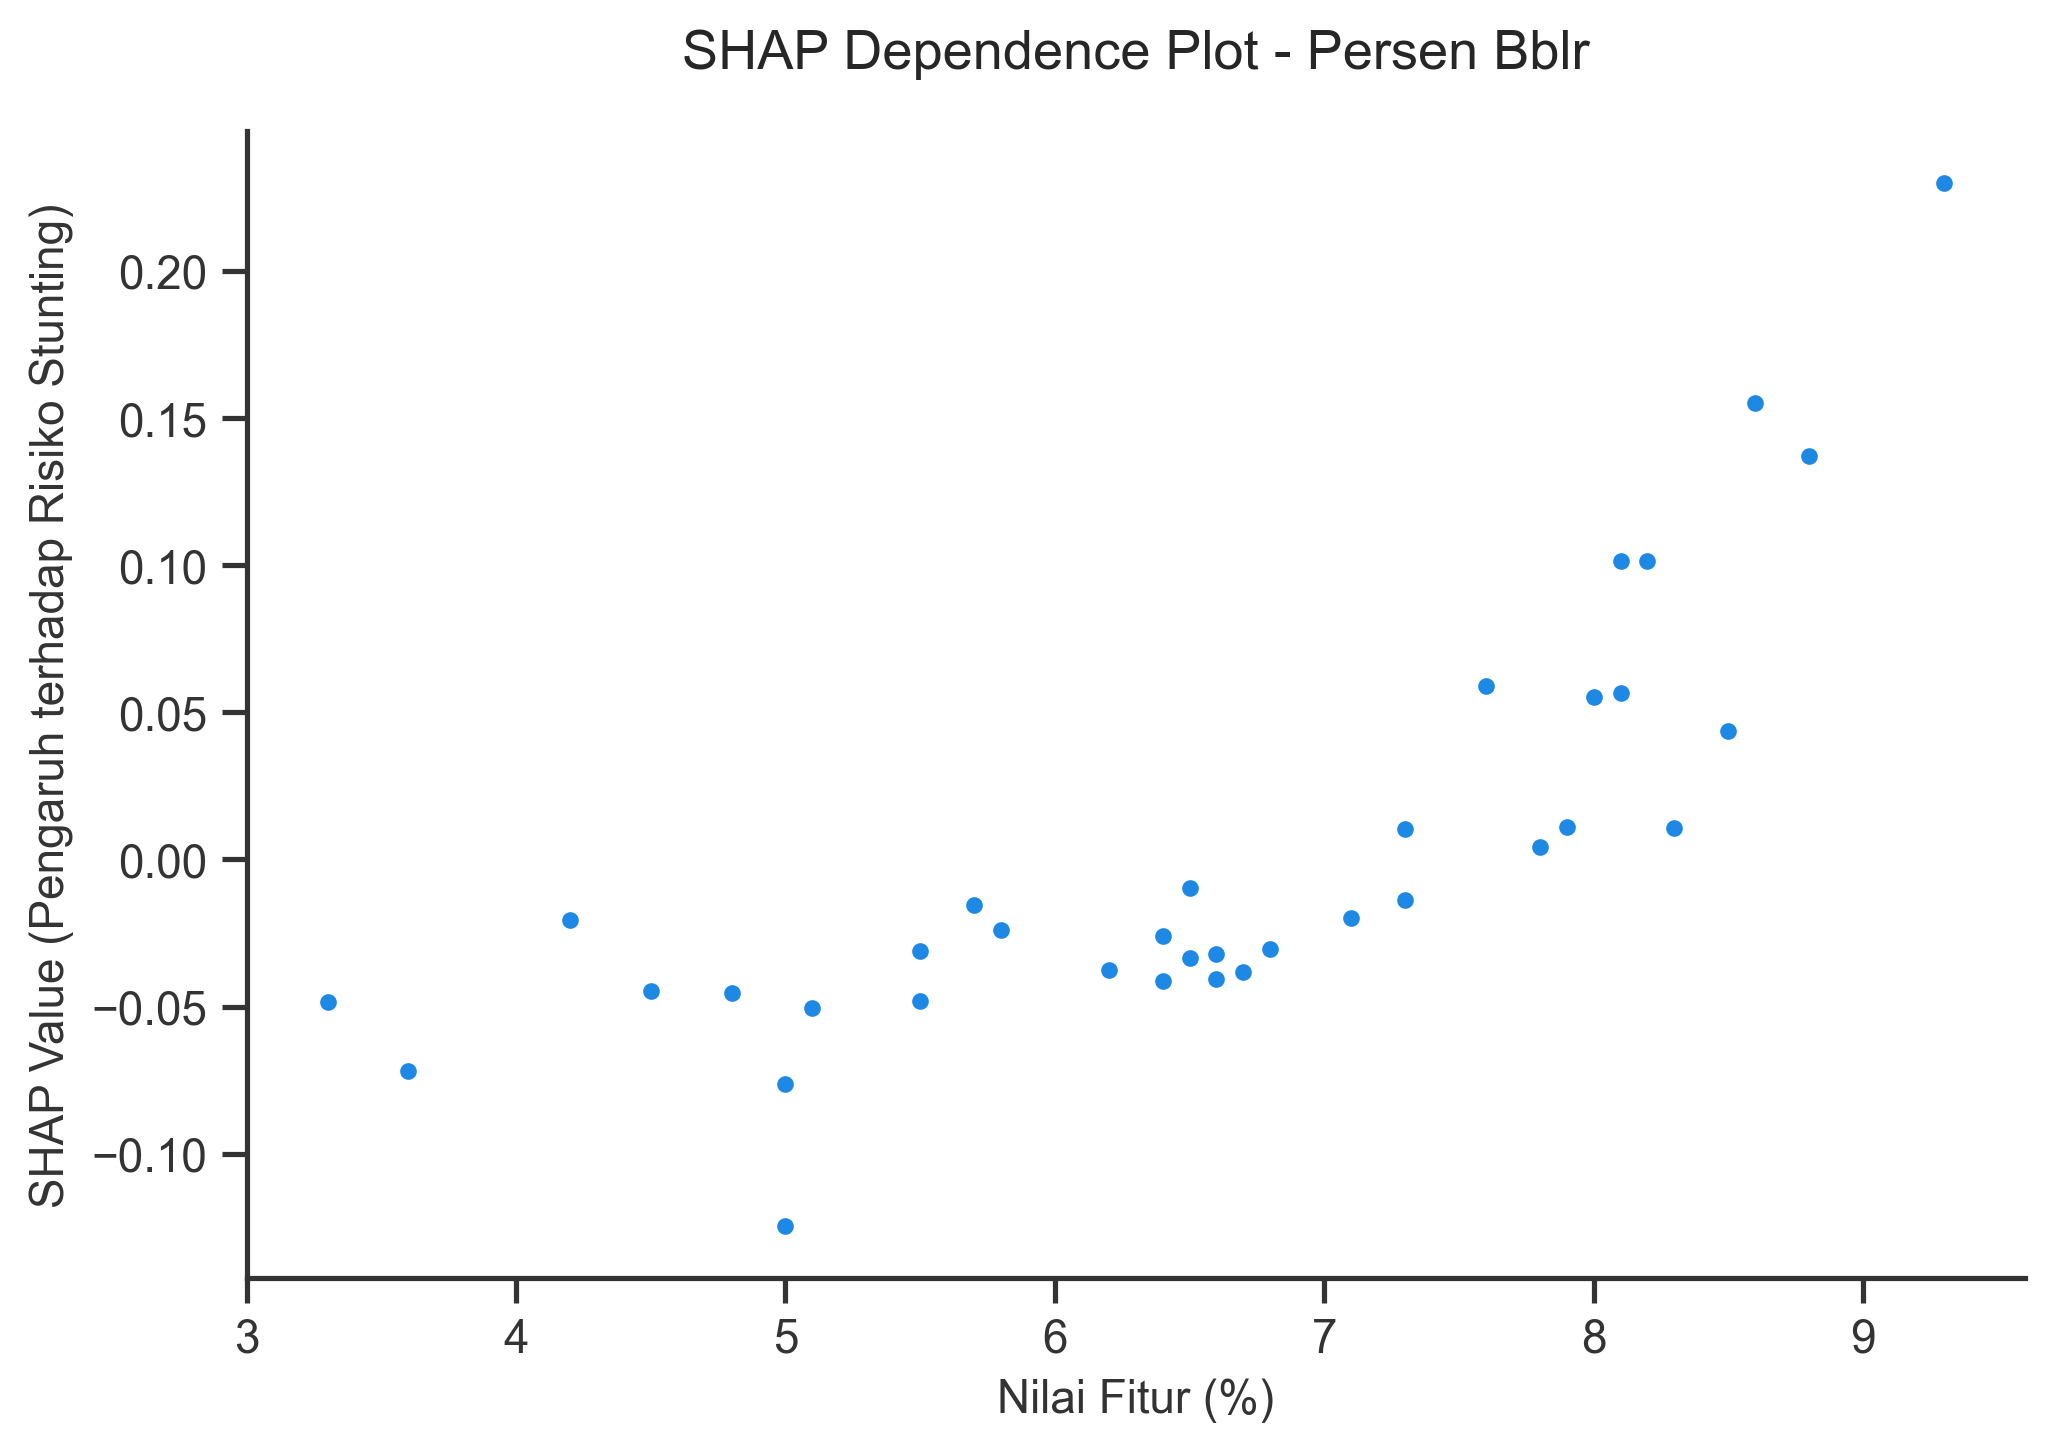
\includegraphics[width=0.48\textwidth]{figure/hasil_dependence_plot/dependence_persen_bblr.png} \\ \vspace{0.2cm}
    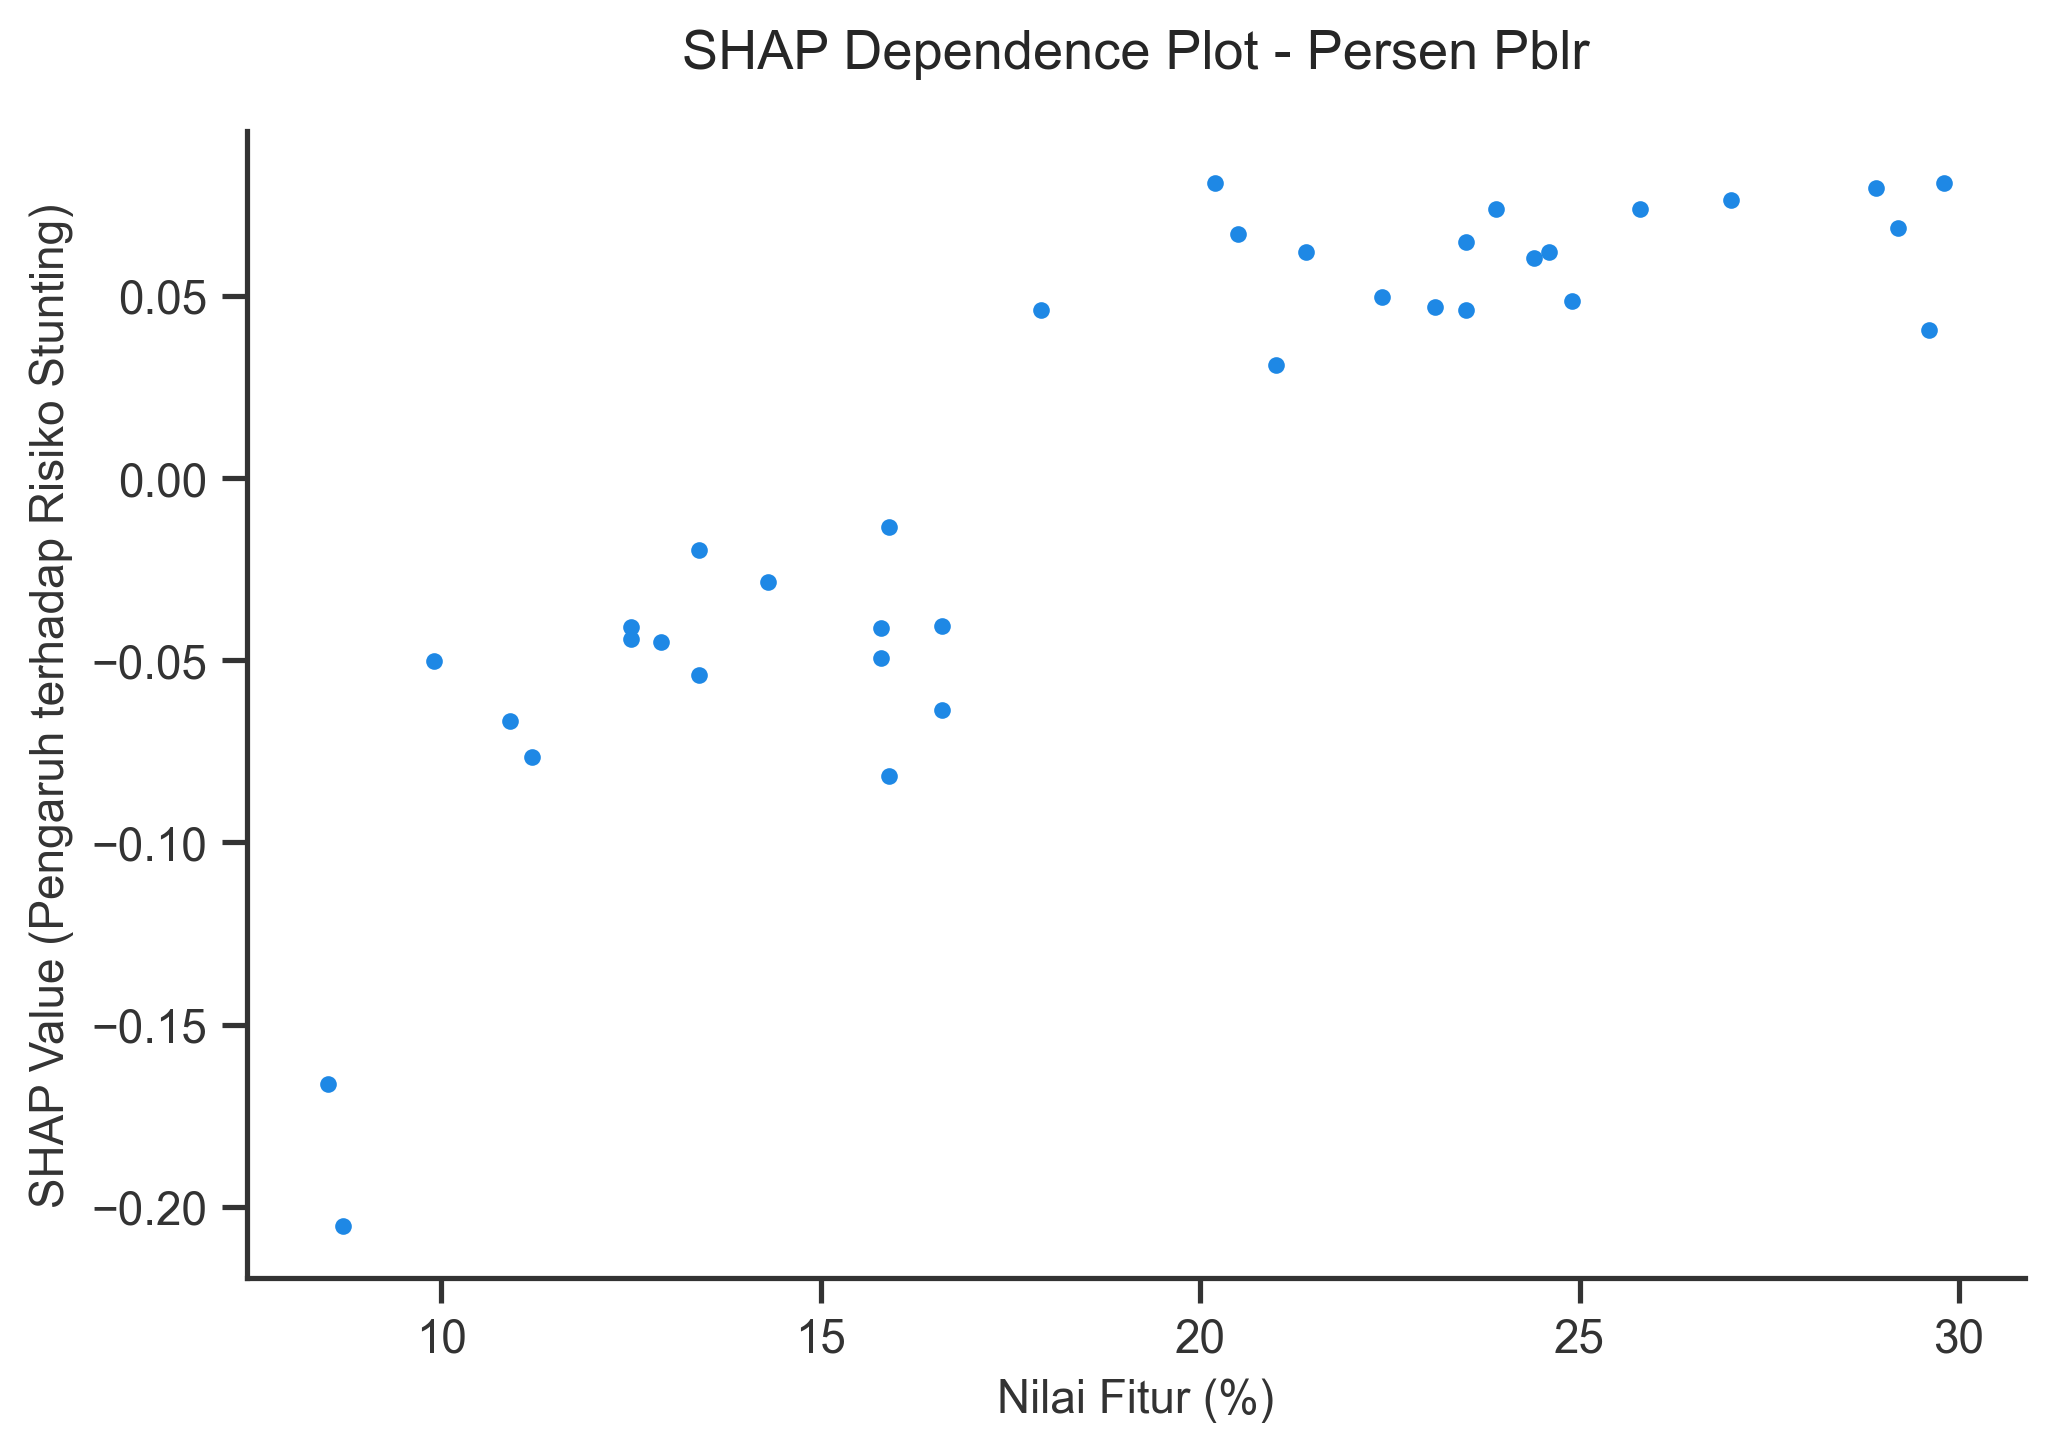
\includegraphics[width=0.48\textwidth]{figure/hasil_dependence_plot/dependence_persen_pblr.png} \hfill
    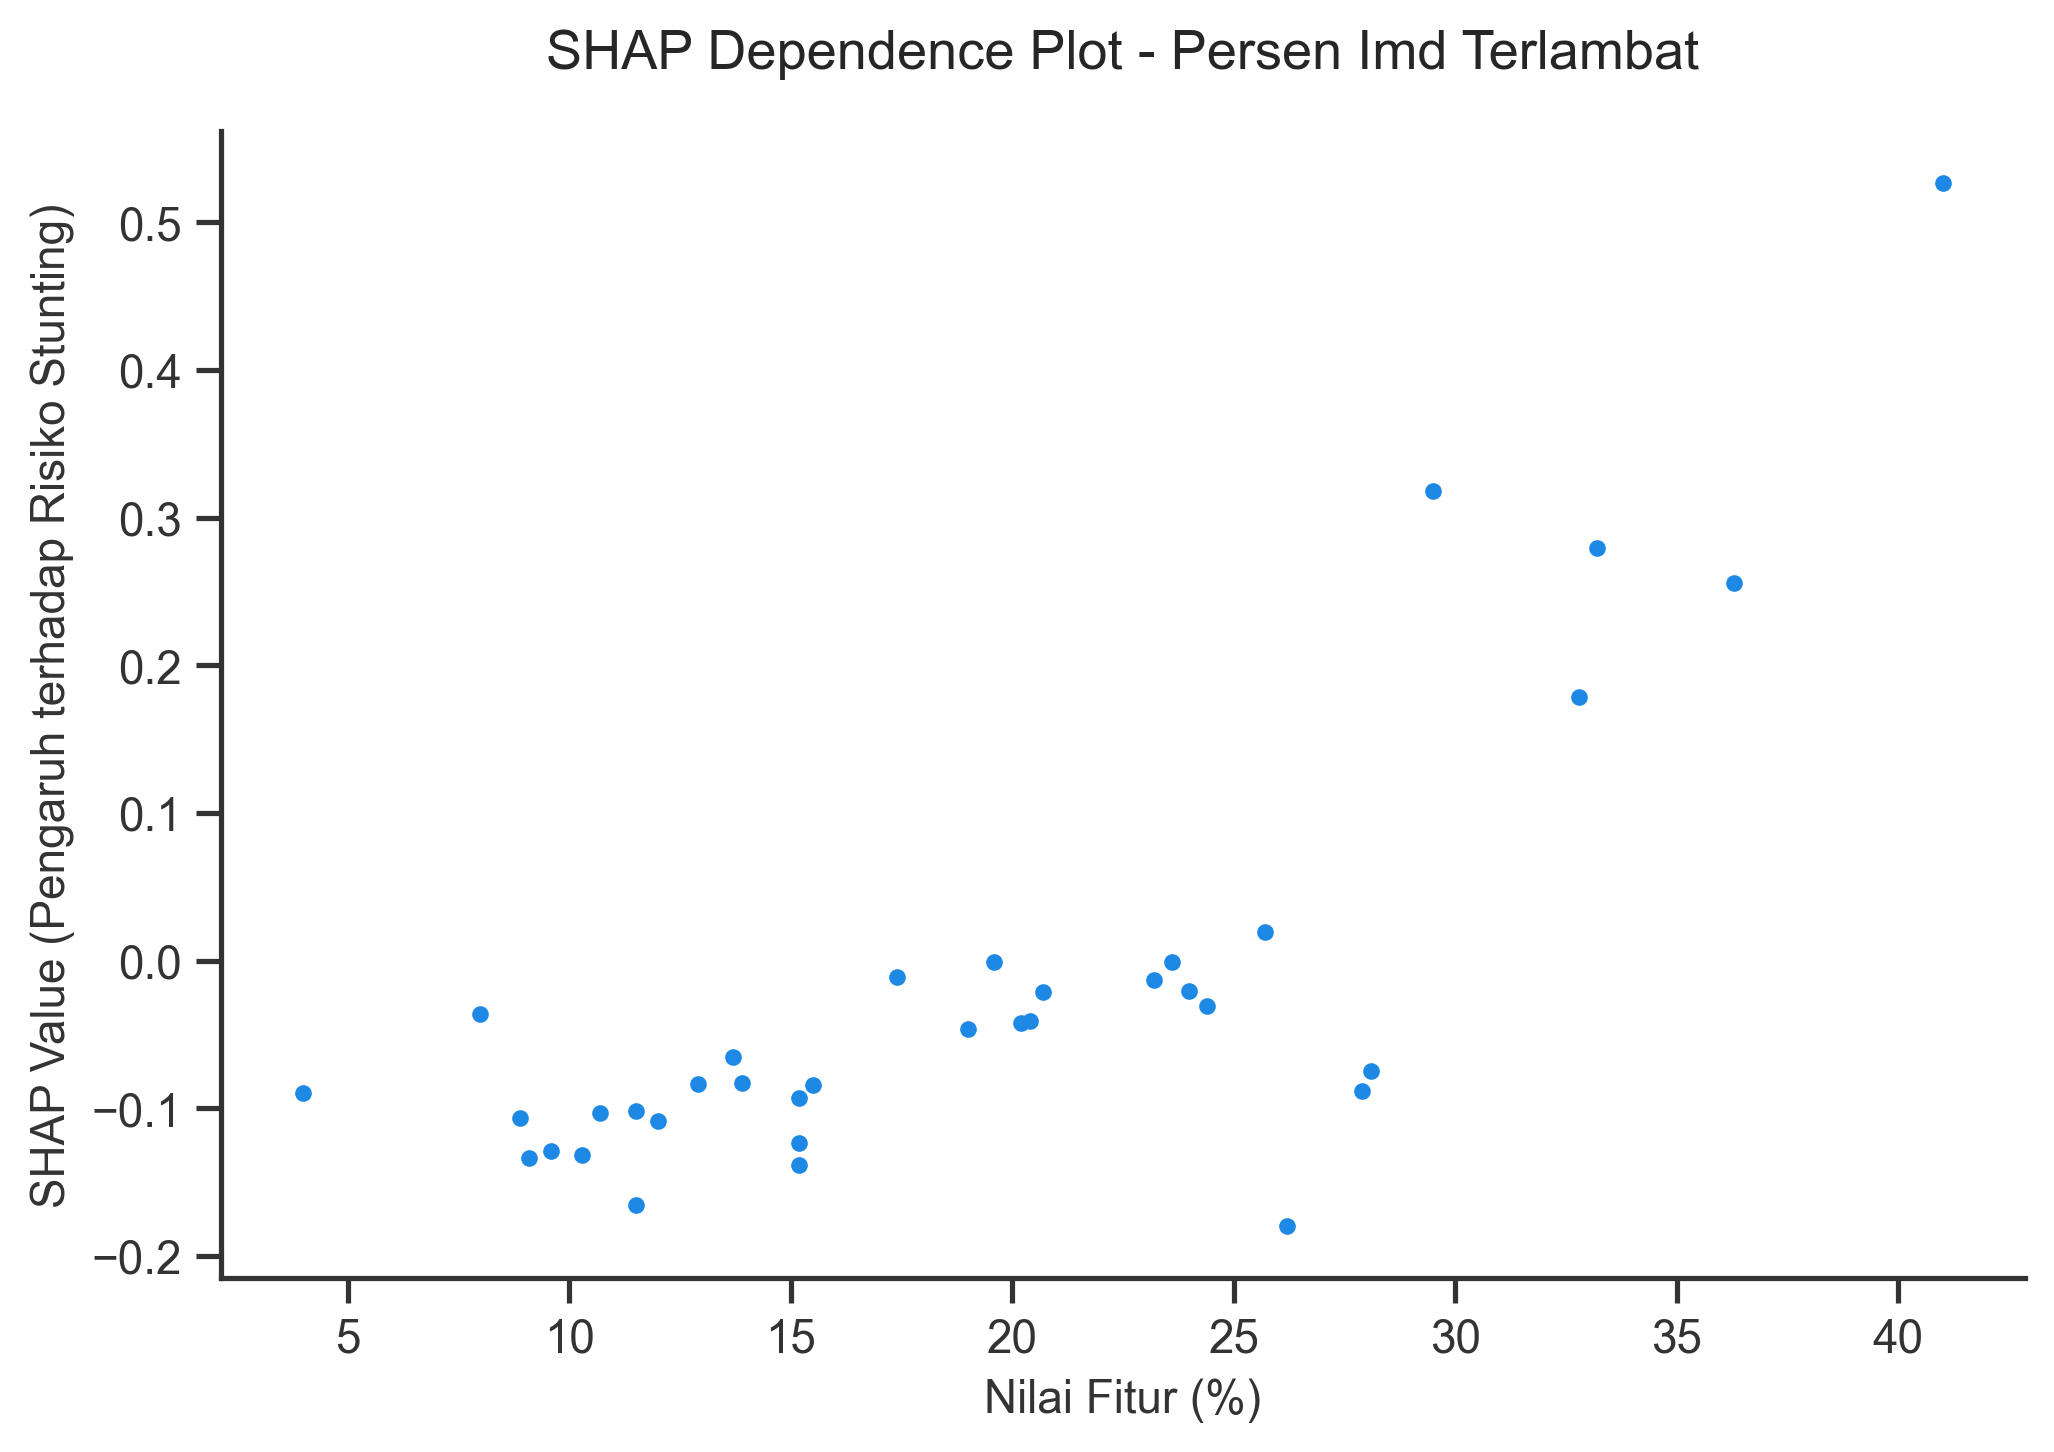
\includegraphics[width=0.48\textwidth]{figure/hasil_dependence_plot/dependence_persen_imd_terlambat.png} \\ \vspace{0.2cm}
    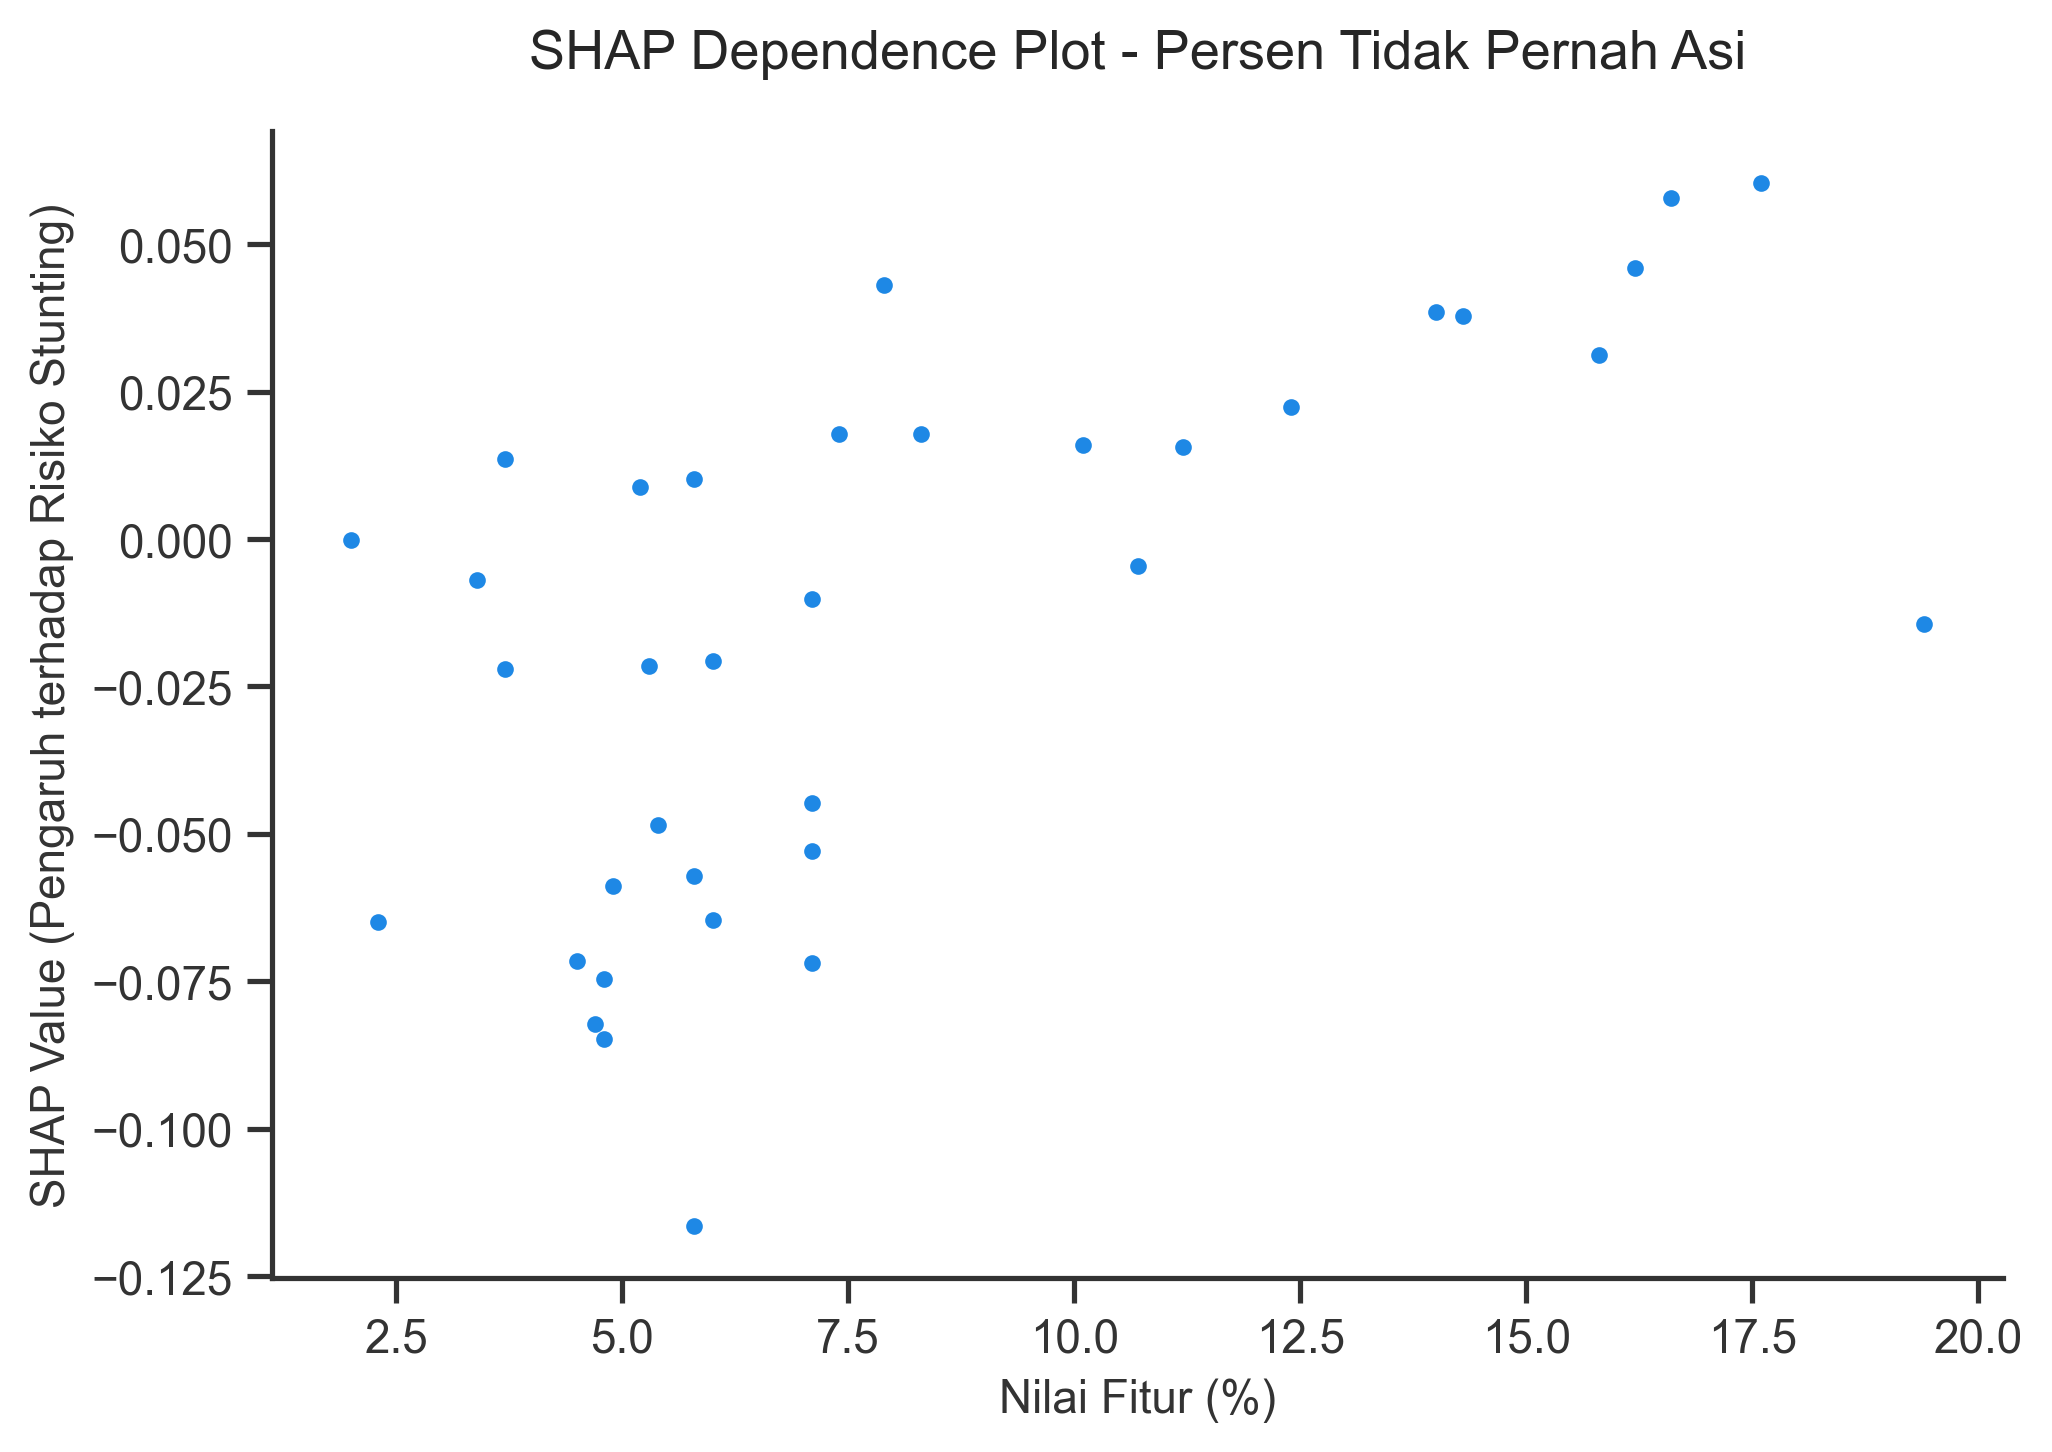
\includegraphics[width=0.48\textwidth]{figure/hasil_dependence_plot/dependence_persen_tidak_pernah_asi.png} \hfill
    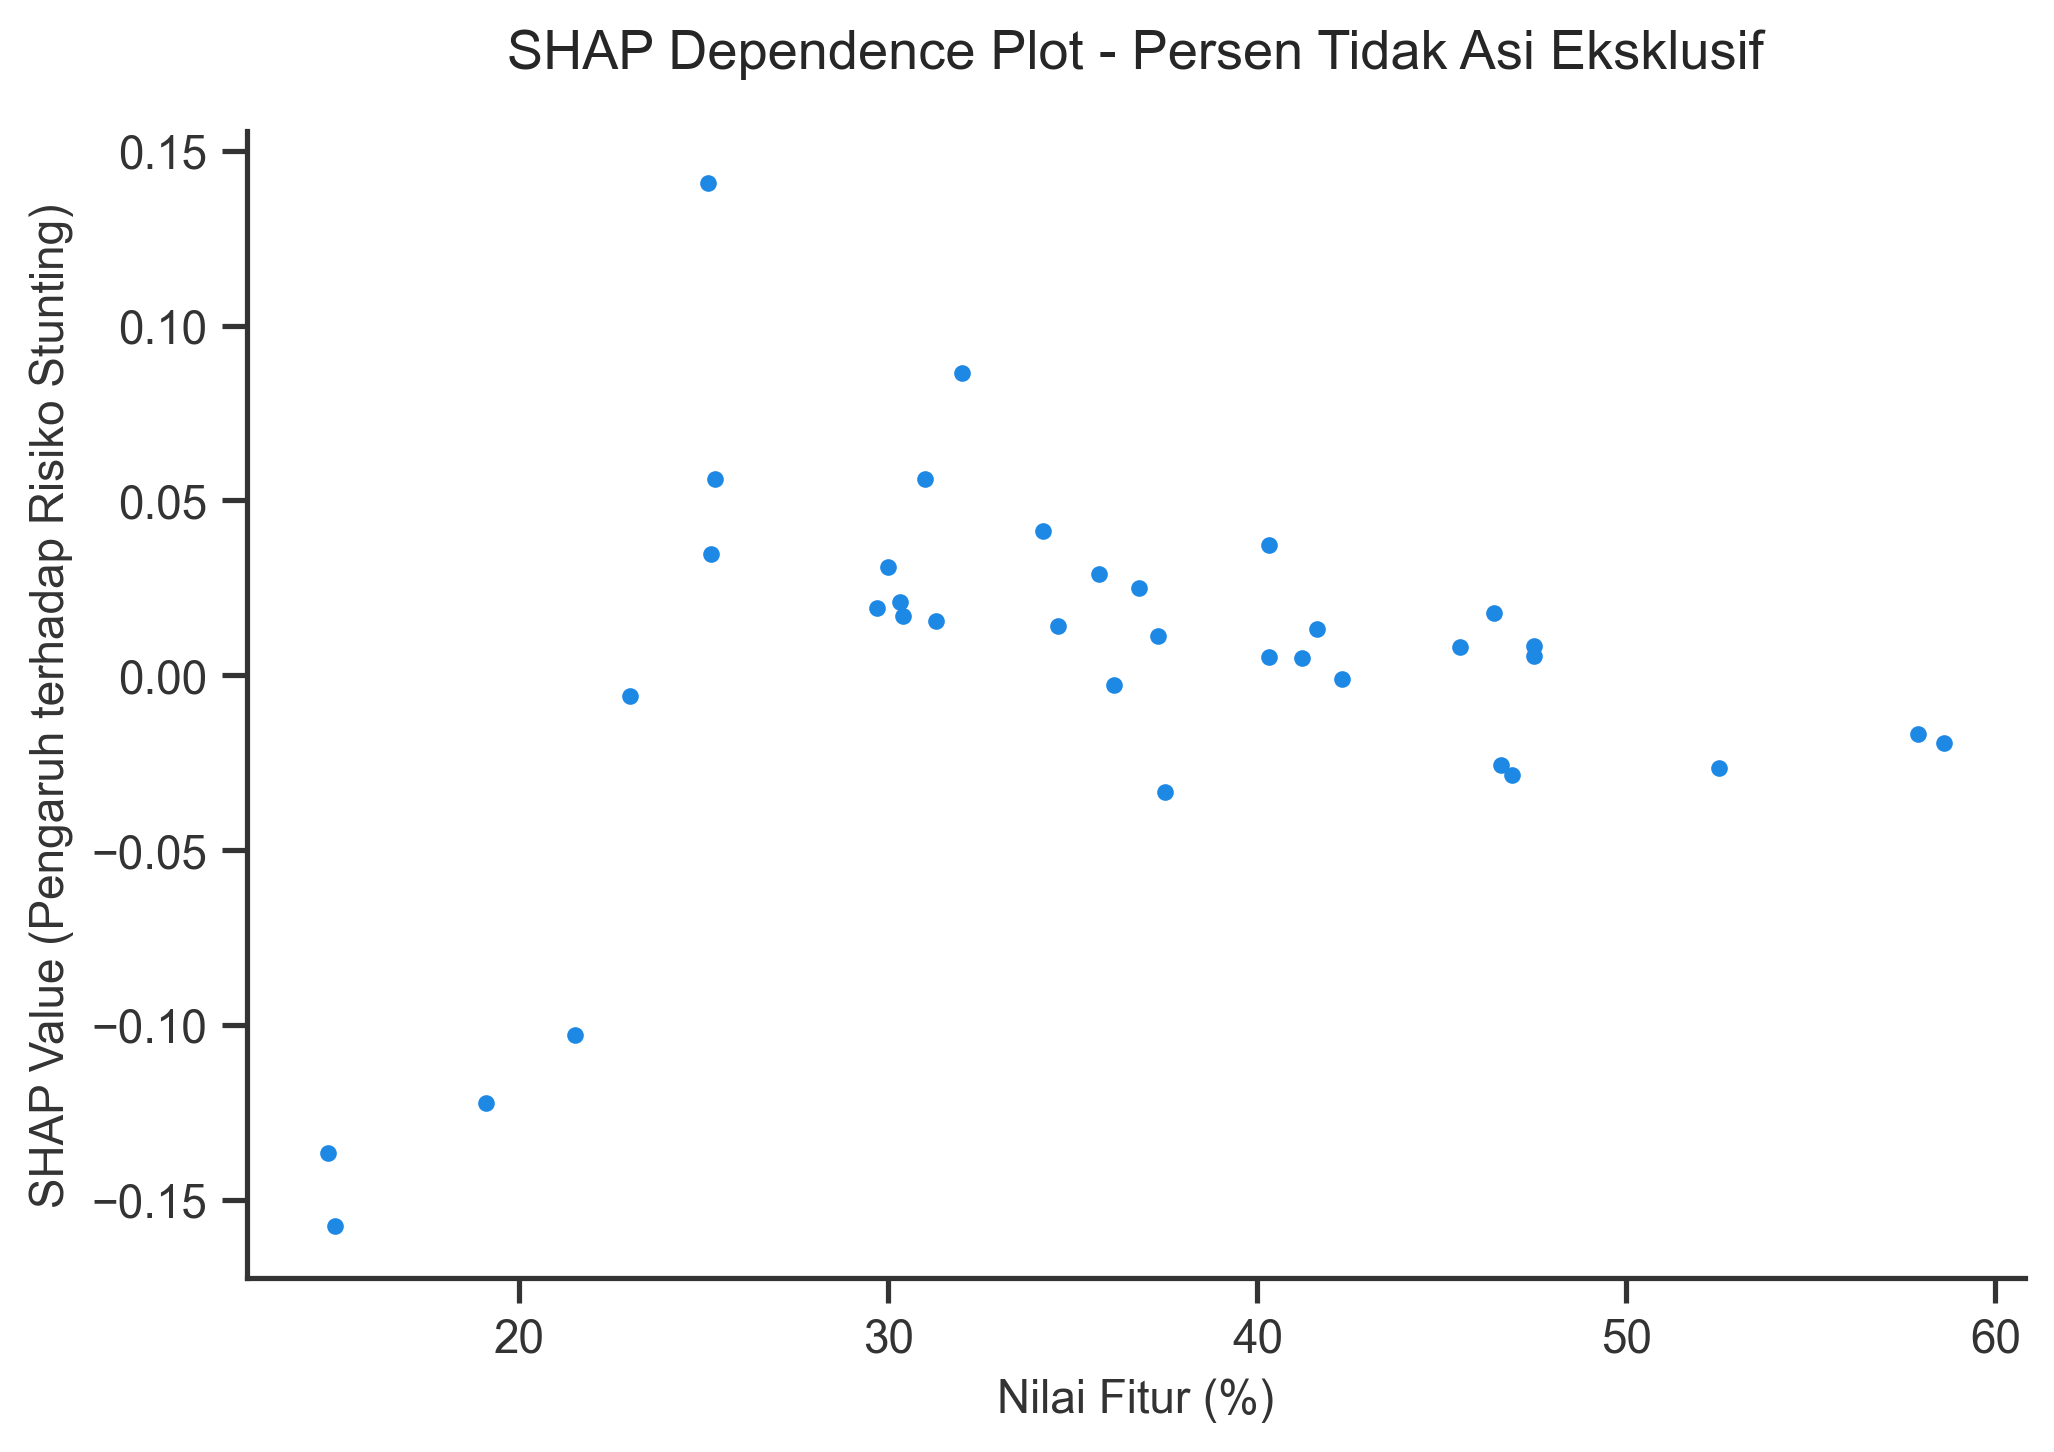
\includegraphics[width=0.48\textwidth]{figure/hasil_dependence_plot/dependence_persen_tidak_asi_eksklusif.png}
\end{figure}

\newpage
\begin{figure}[H]
    \centering
    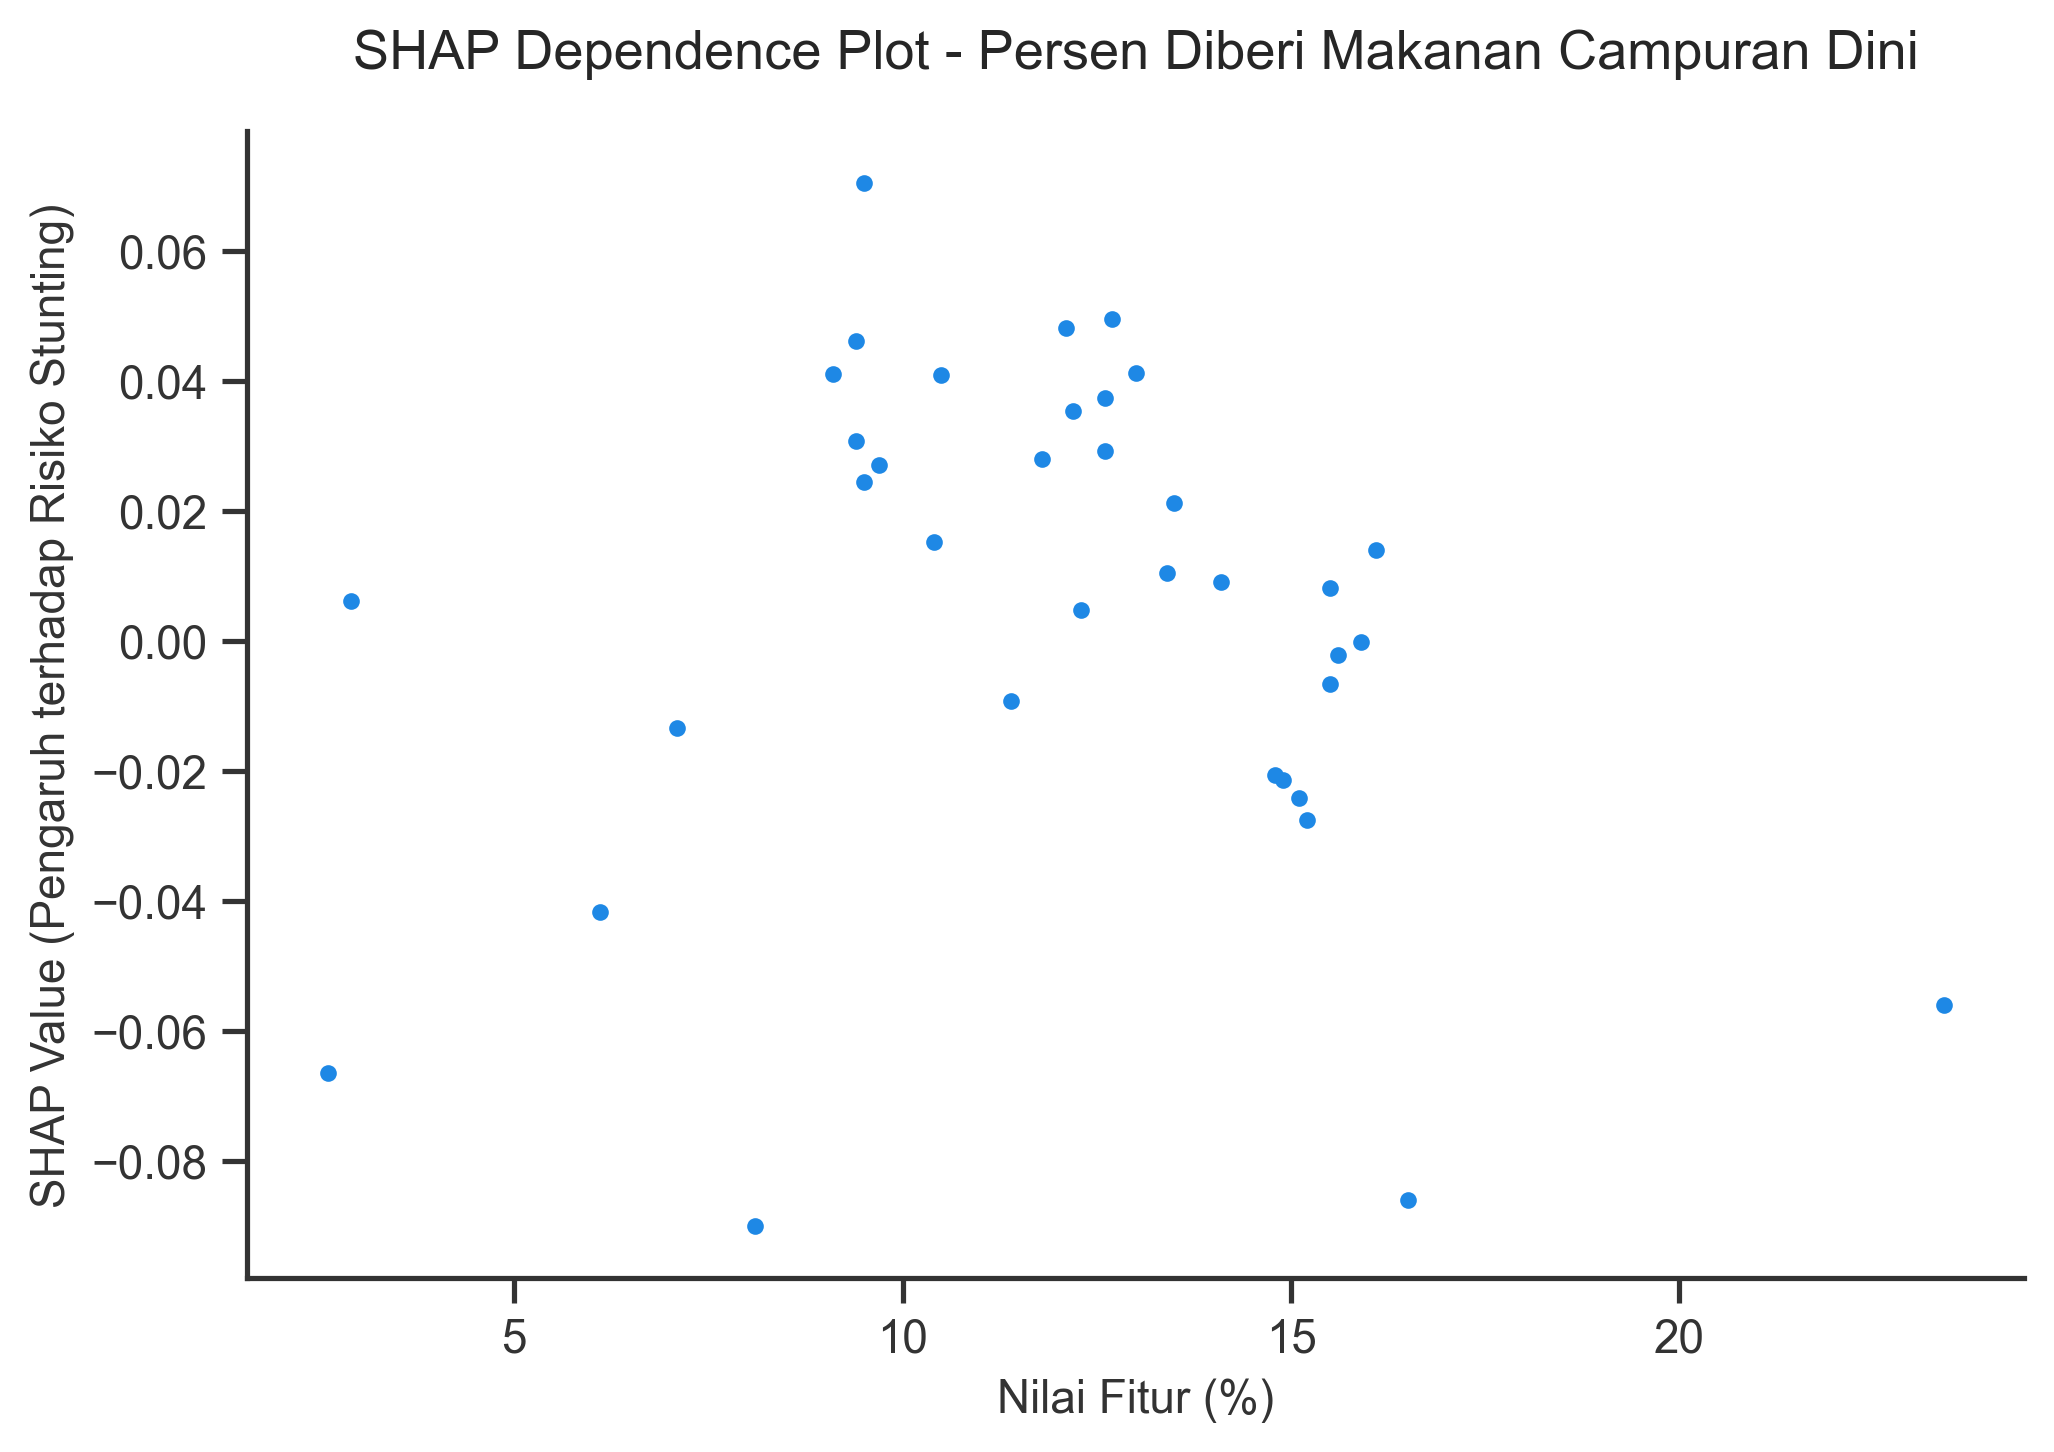
\includegraphics[width=0.48\textwidth]{figure/hasil_dependence_plot/dependence_persen_diberi_makanan_campuran_dini.png} \hfill
    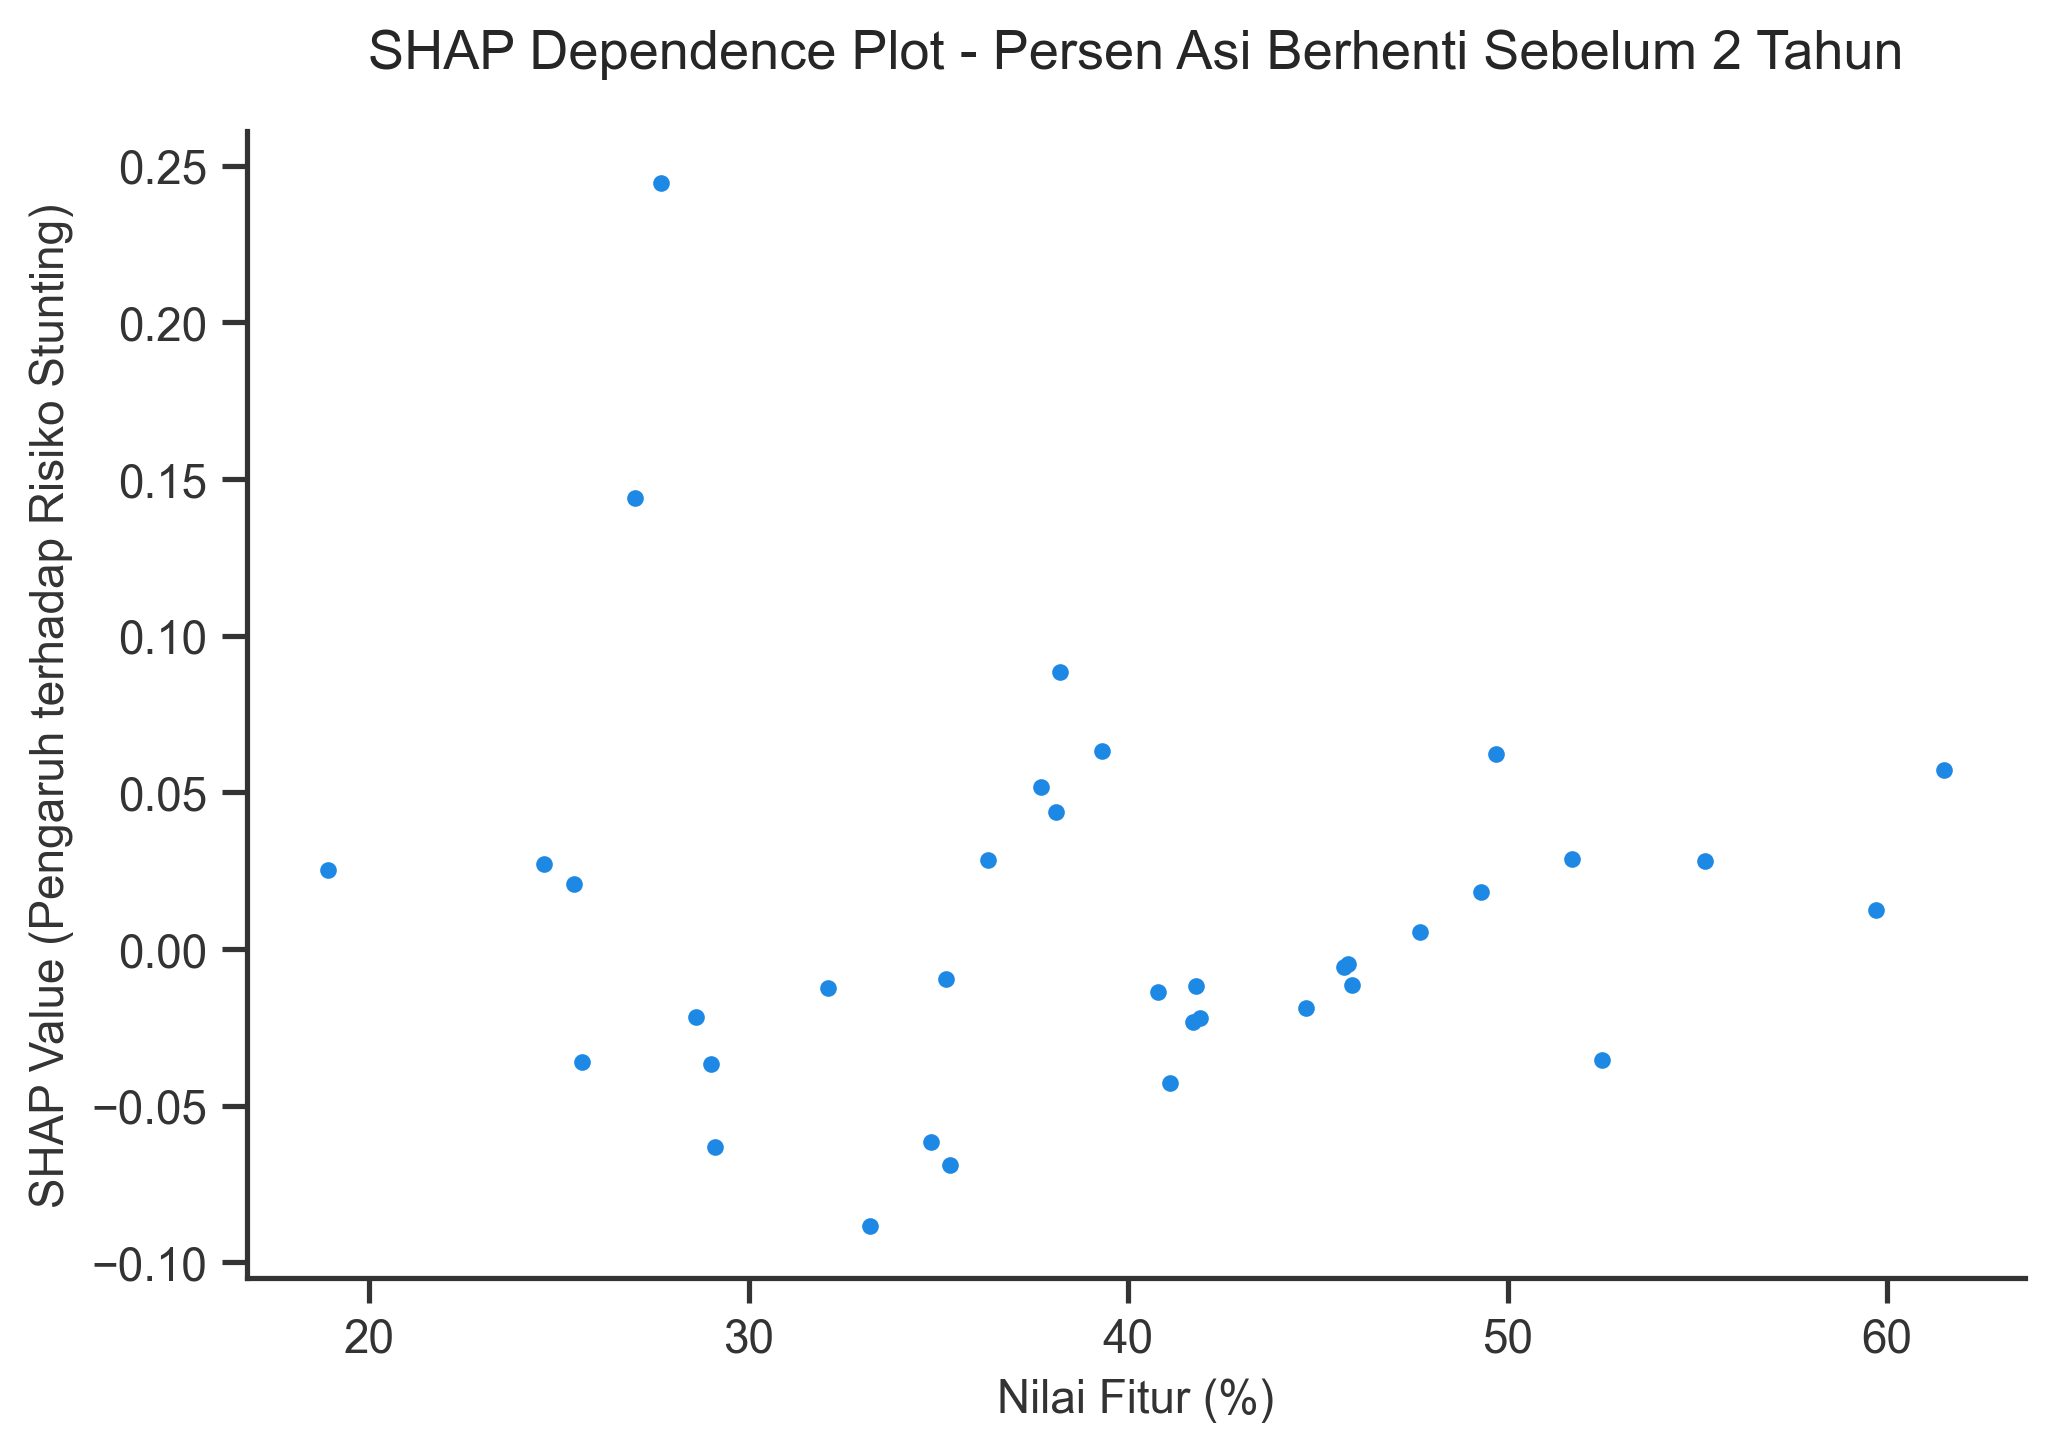
\includegraphics[width=0.48\textwidth]{figure/hasil_dependence_plot/dependence_persen_asi_berhenti_sebelum_2_tahun.png} \\ \vspace{0.2cm}
    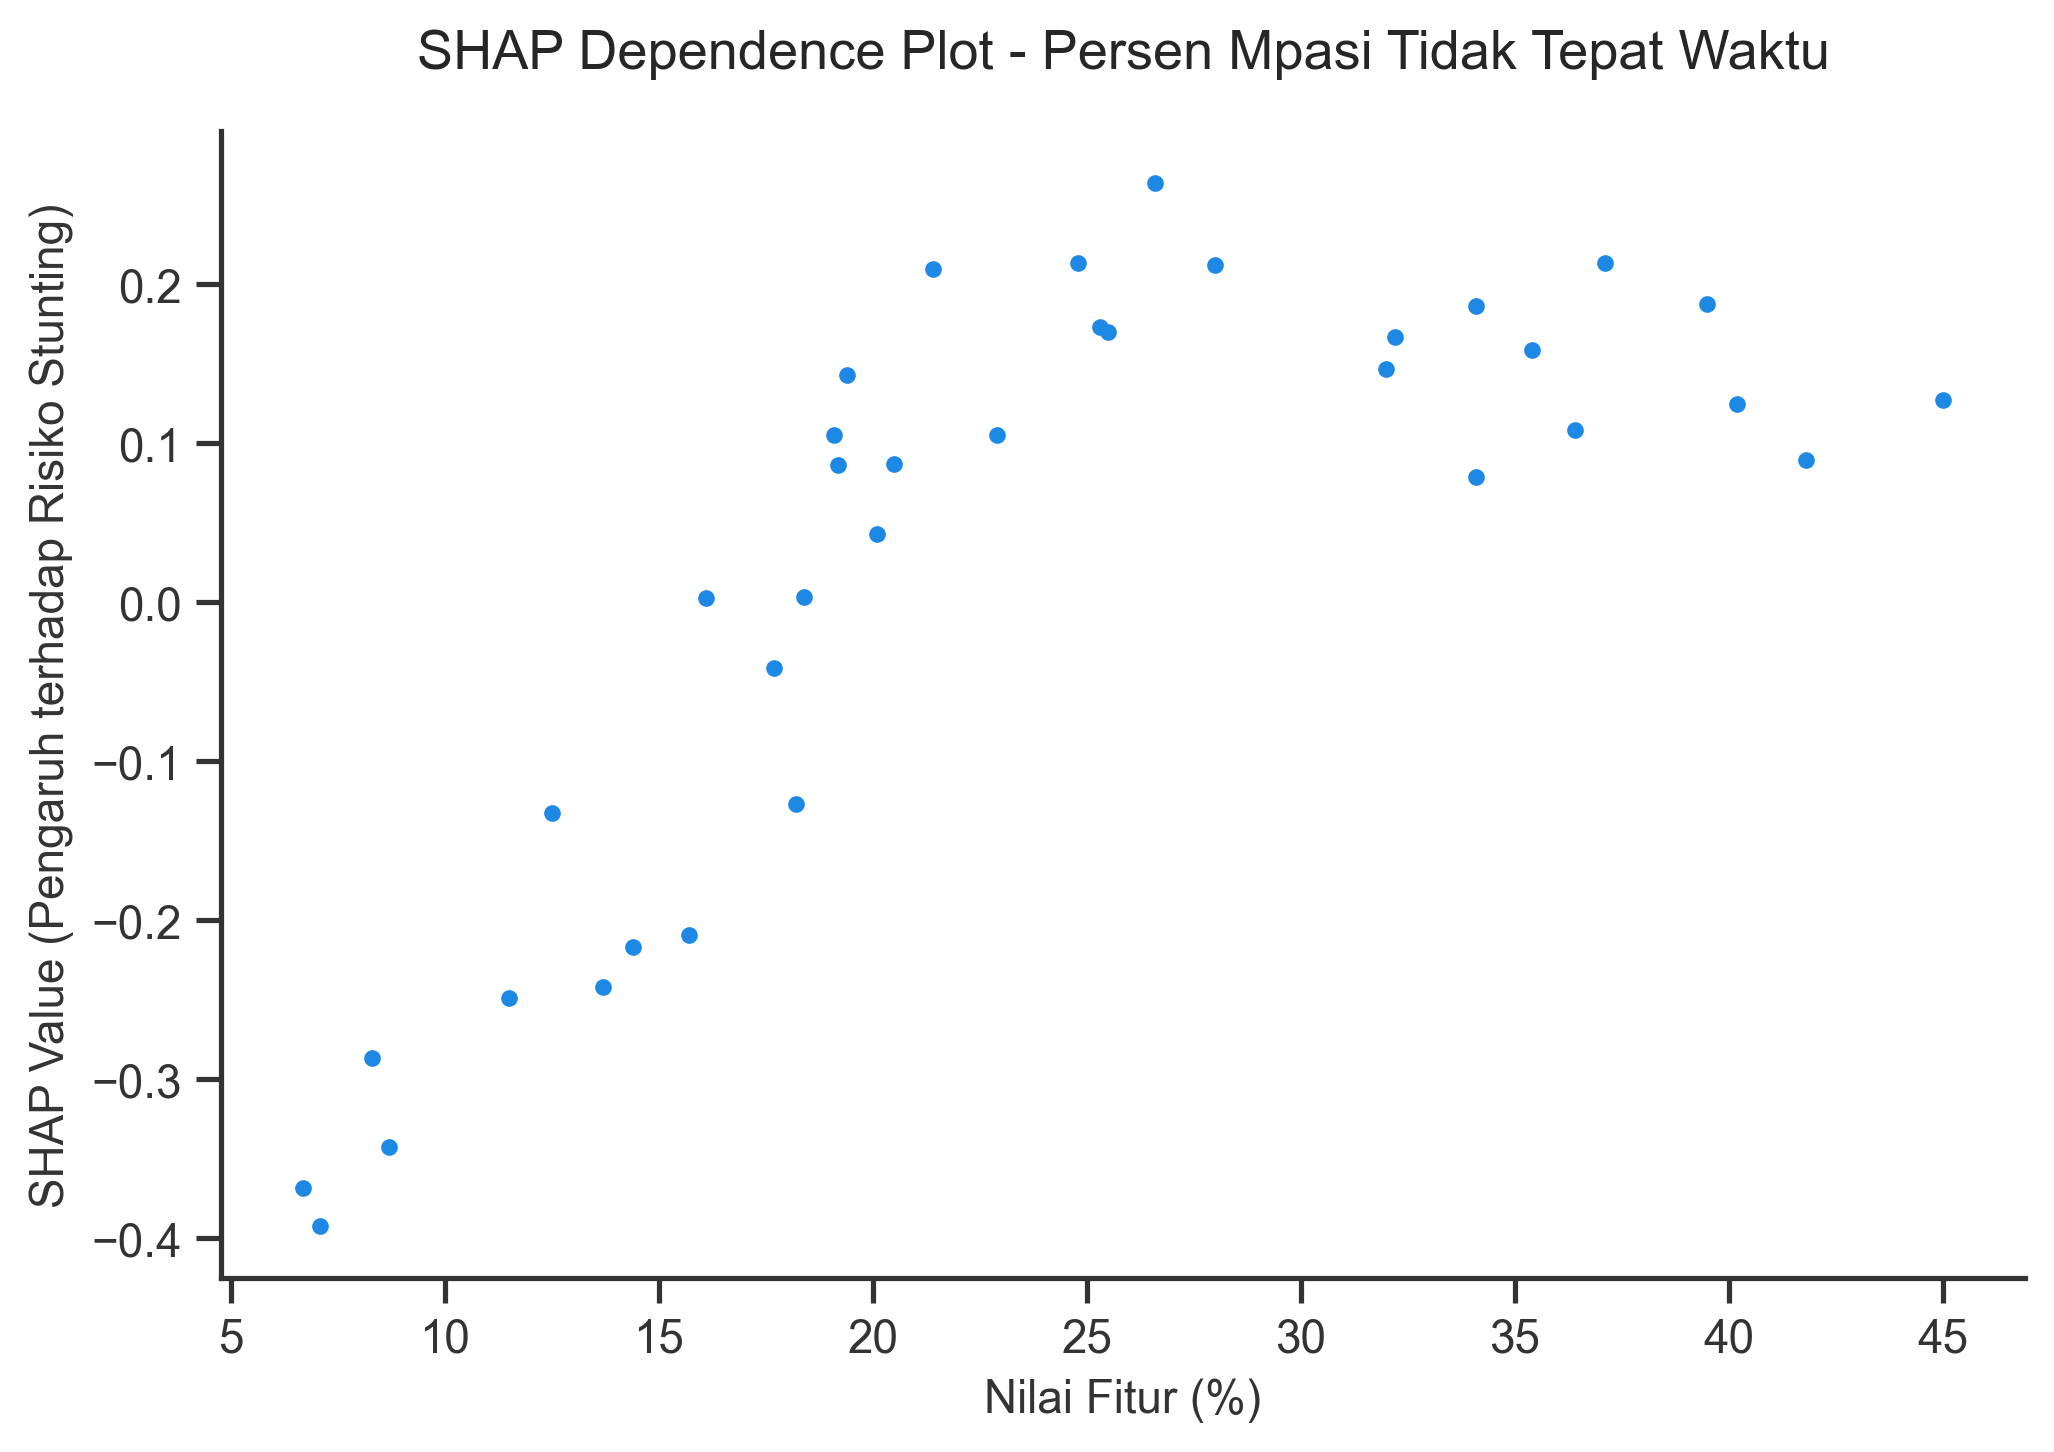
\includegraphics[width=0.48\textwidth]{figure/hasil_dependence_plot/dependence_persen_mpasi_tidak_tepat_waktu.png} \hfill
    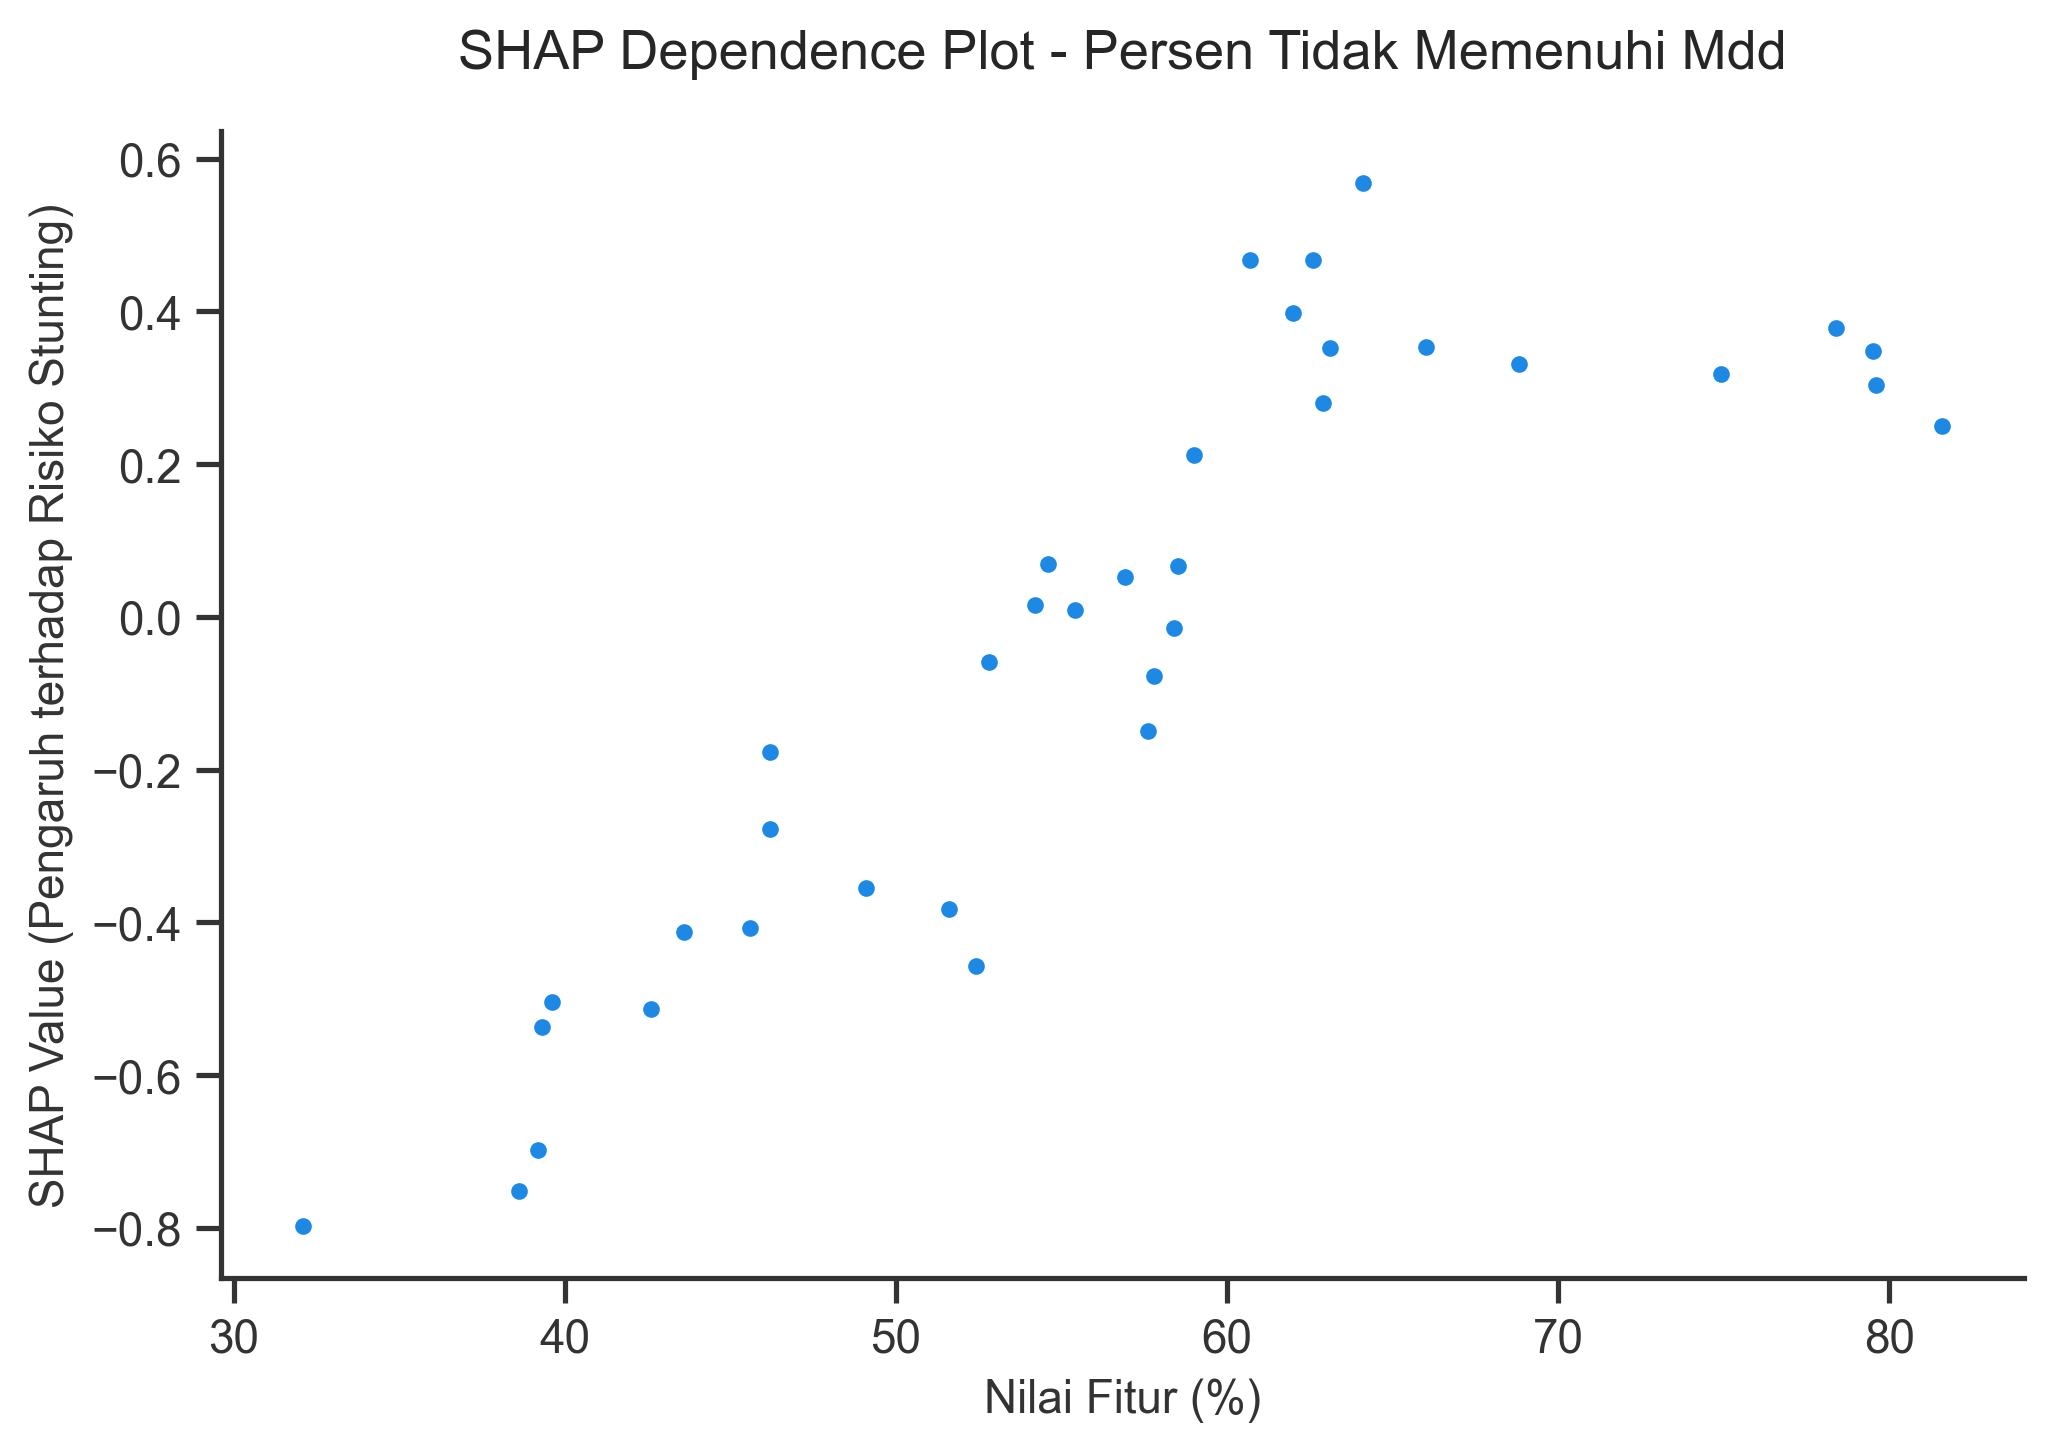
\includegraphics[width=0.48\textwidth]{figure/hasil_dependence_plot/dependence_persen_tidak_memenuhi_mdd.png} \\ \vspace{0.2cm}
    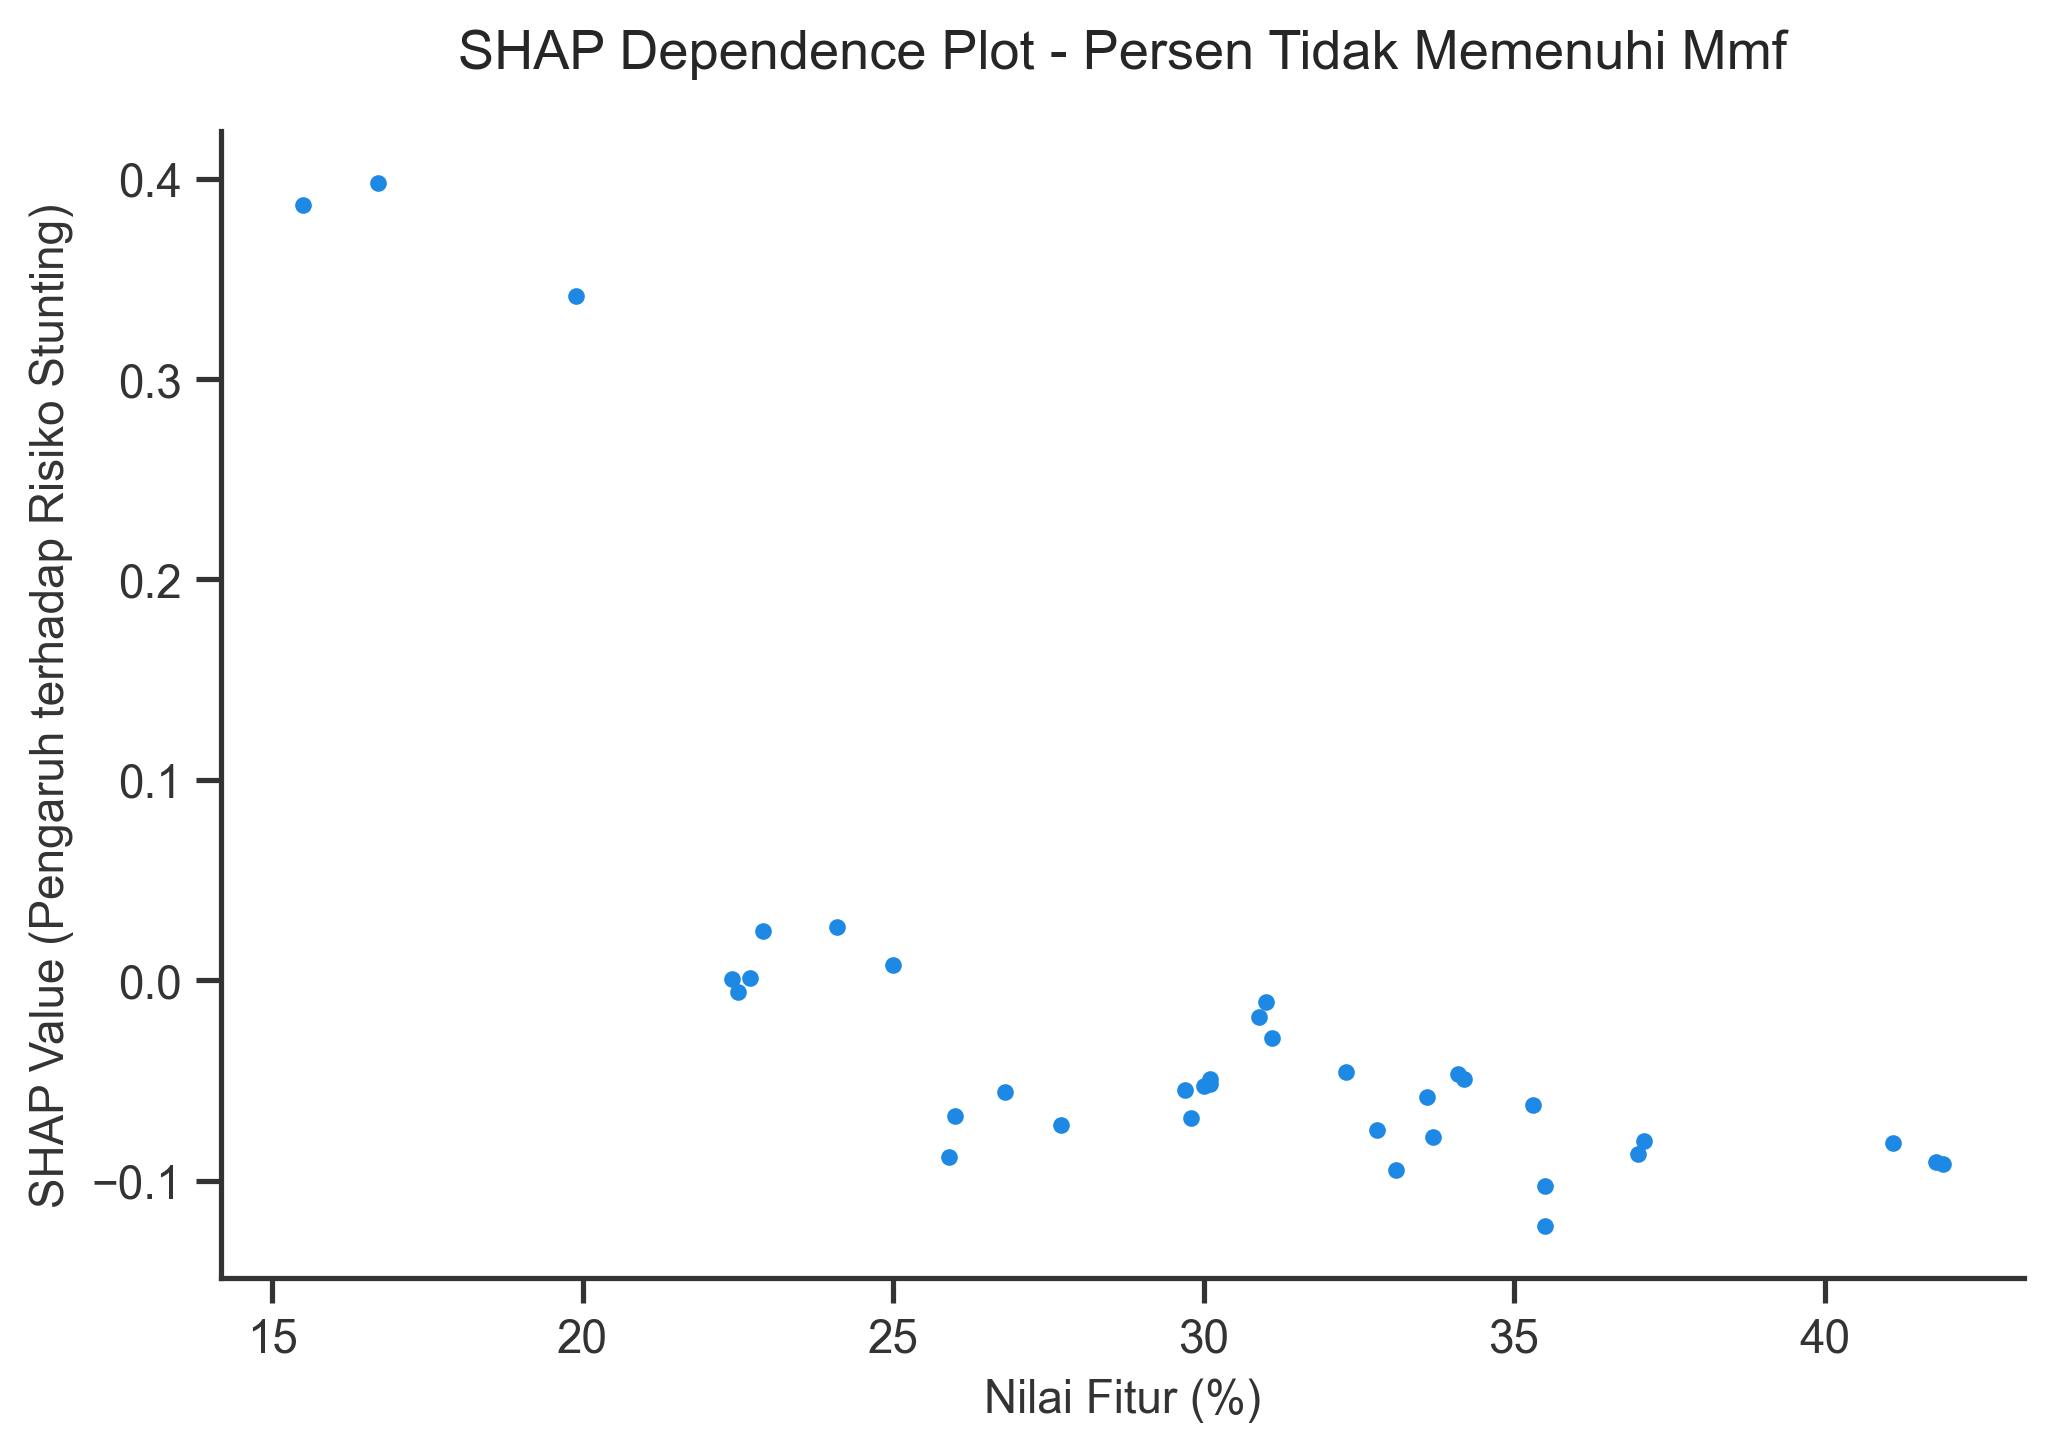
\includegraphics[width=0.48\textwidth]{figure/hasil_dependence_plot/dependence_persen_tidak_memenuhi_mmf.png} \hfill
    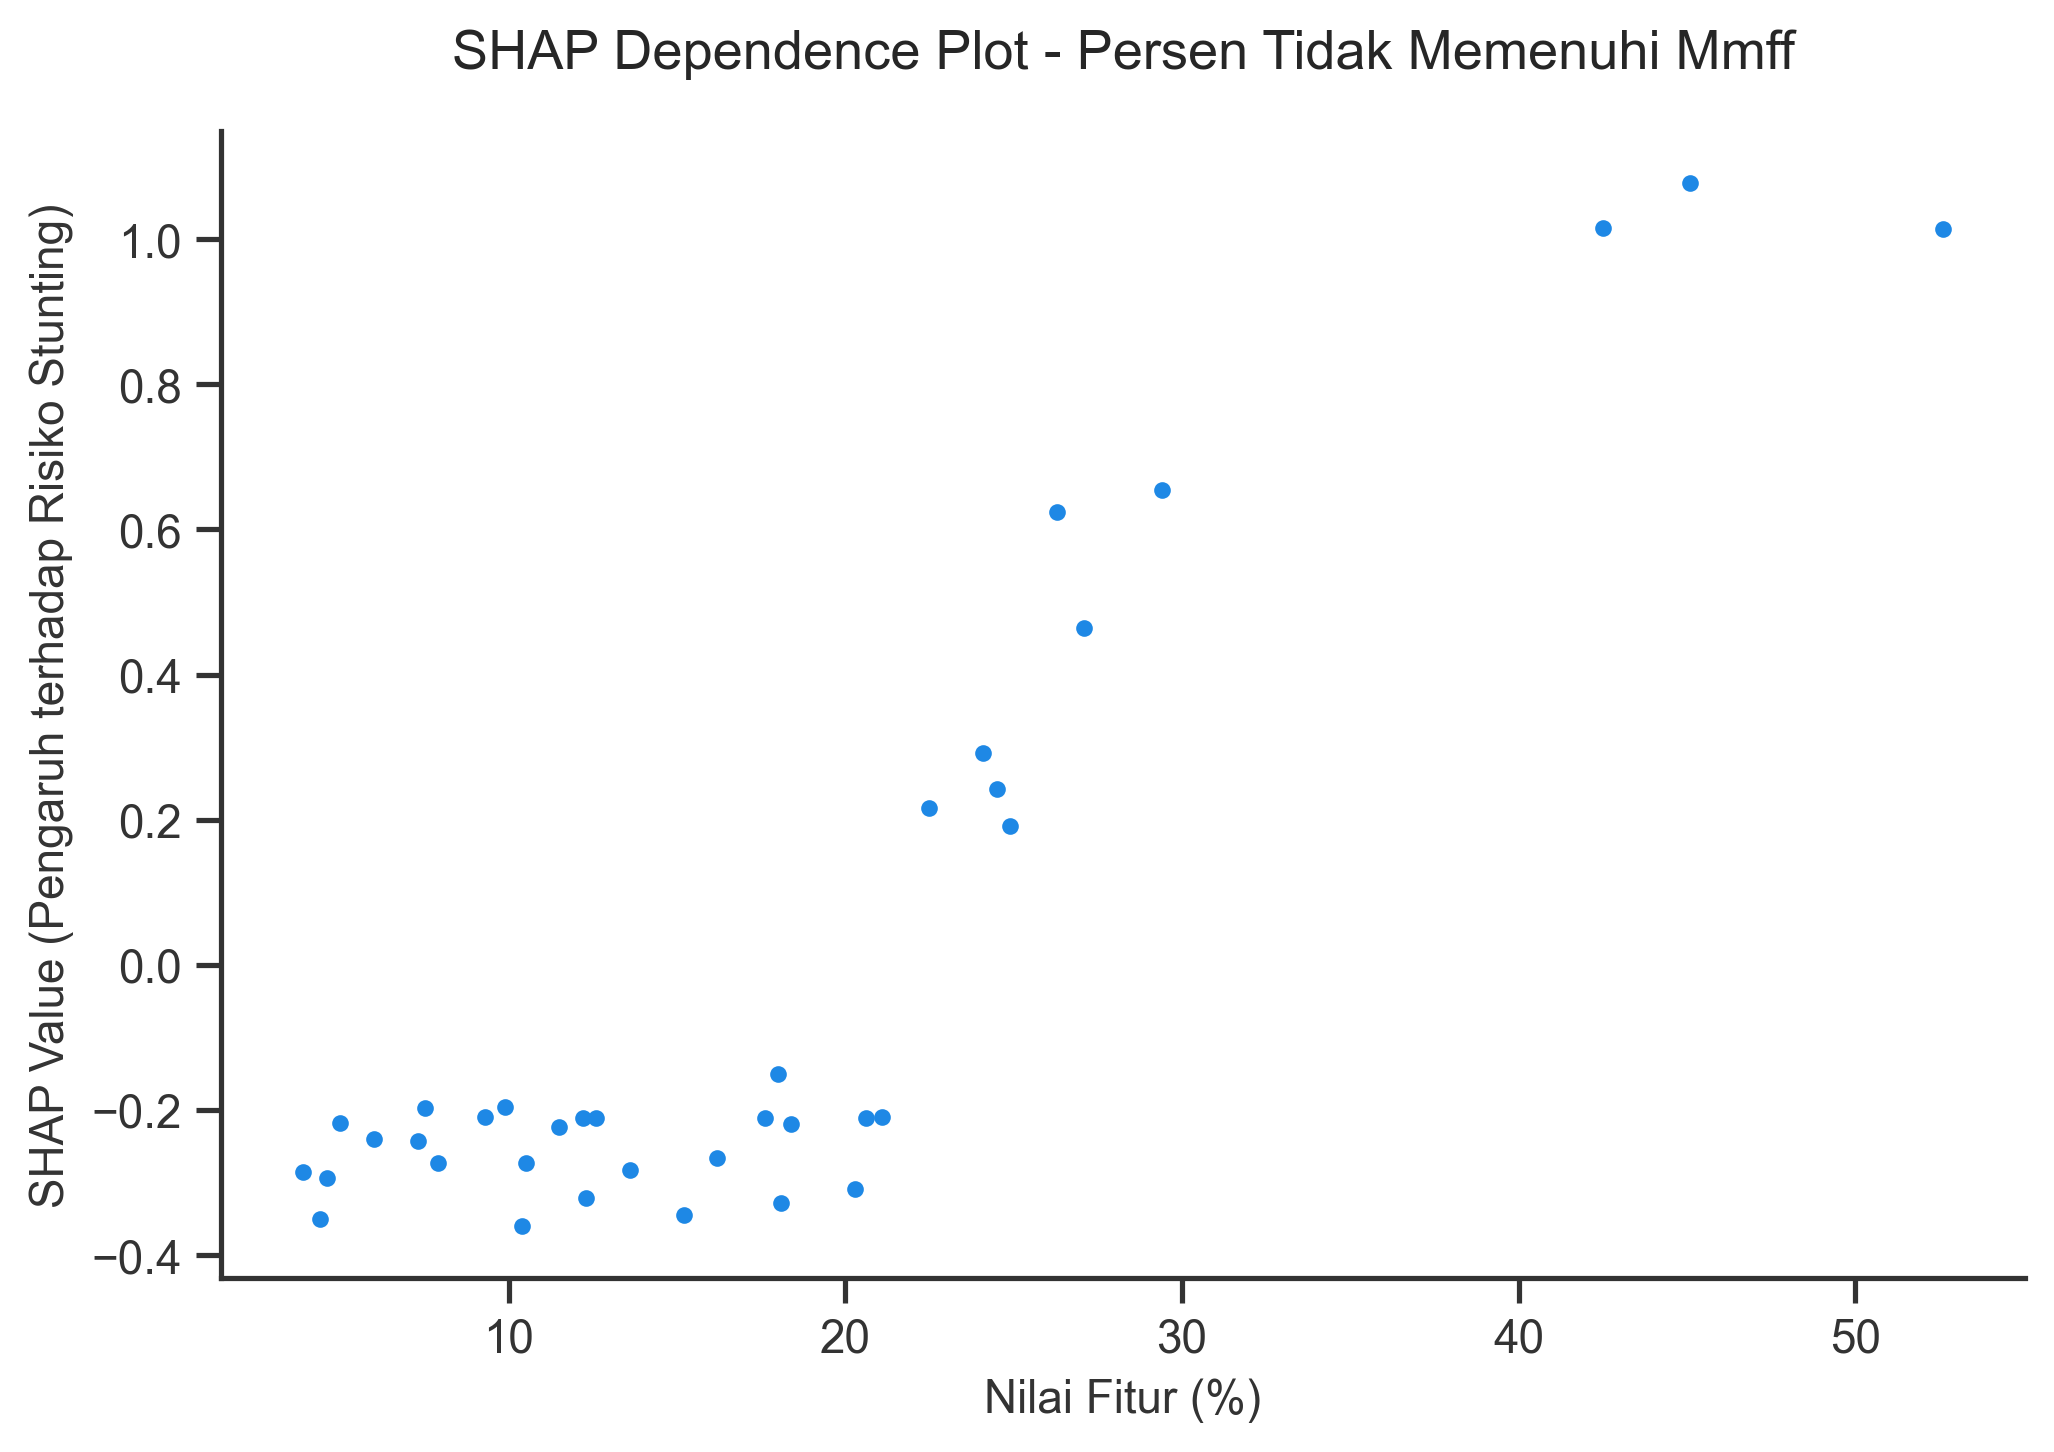
\includegraphics[width=0.48\textwidth]{figure/hasil_dependence_plot/dependence_persen_tidak_memenuhi_mmff.png} \\ \vspace{0.2cm}
    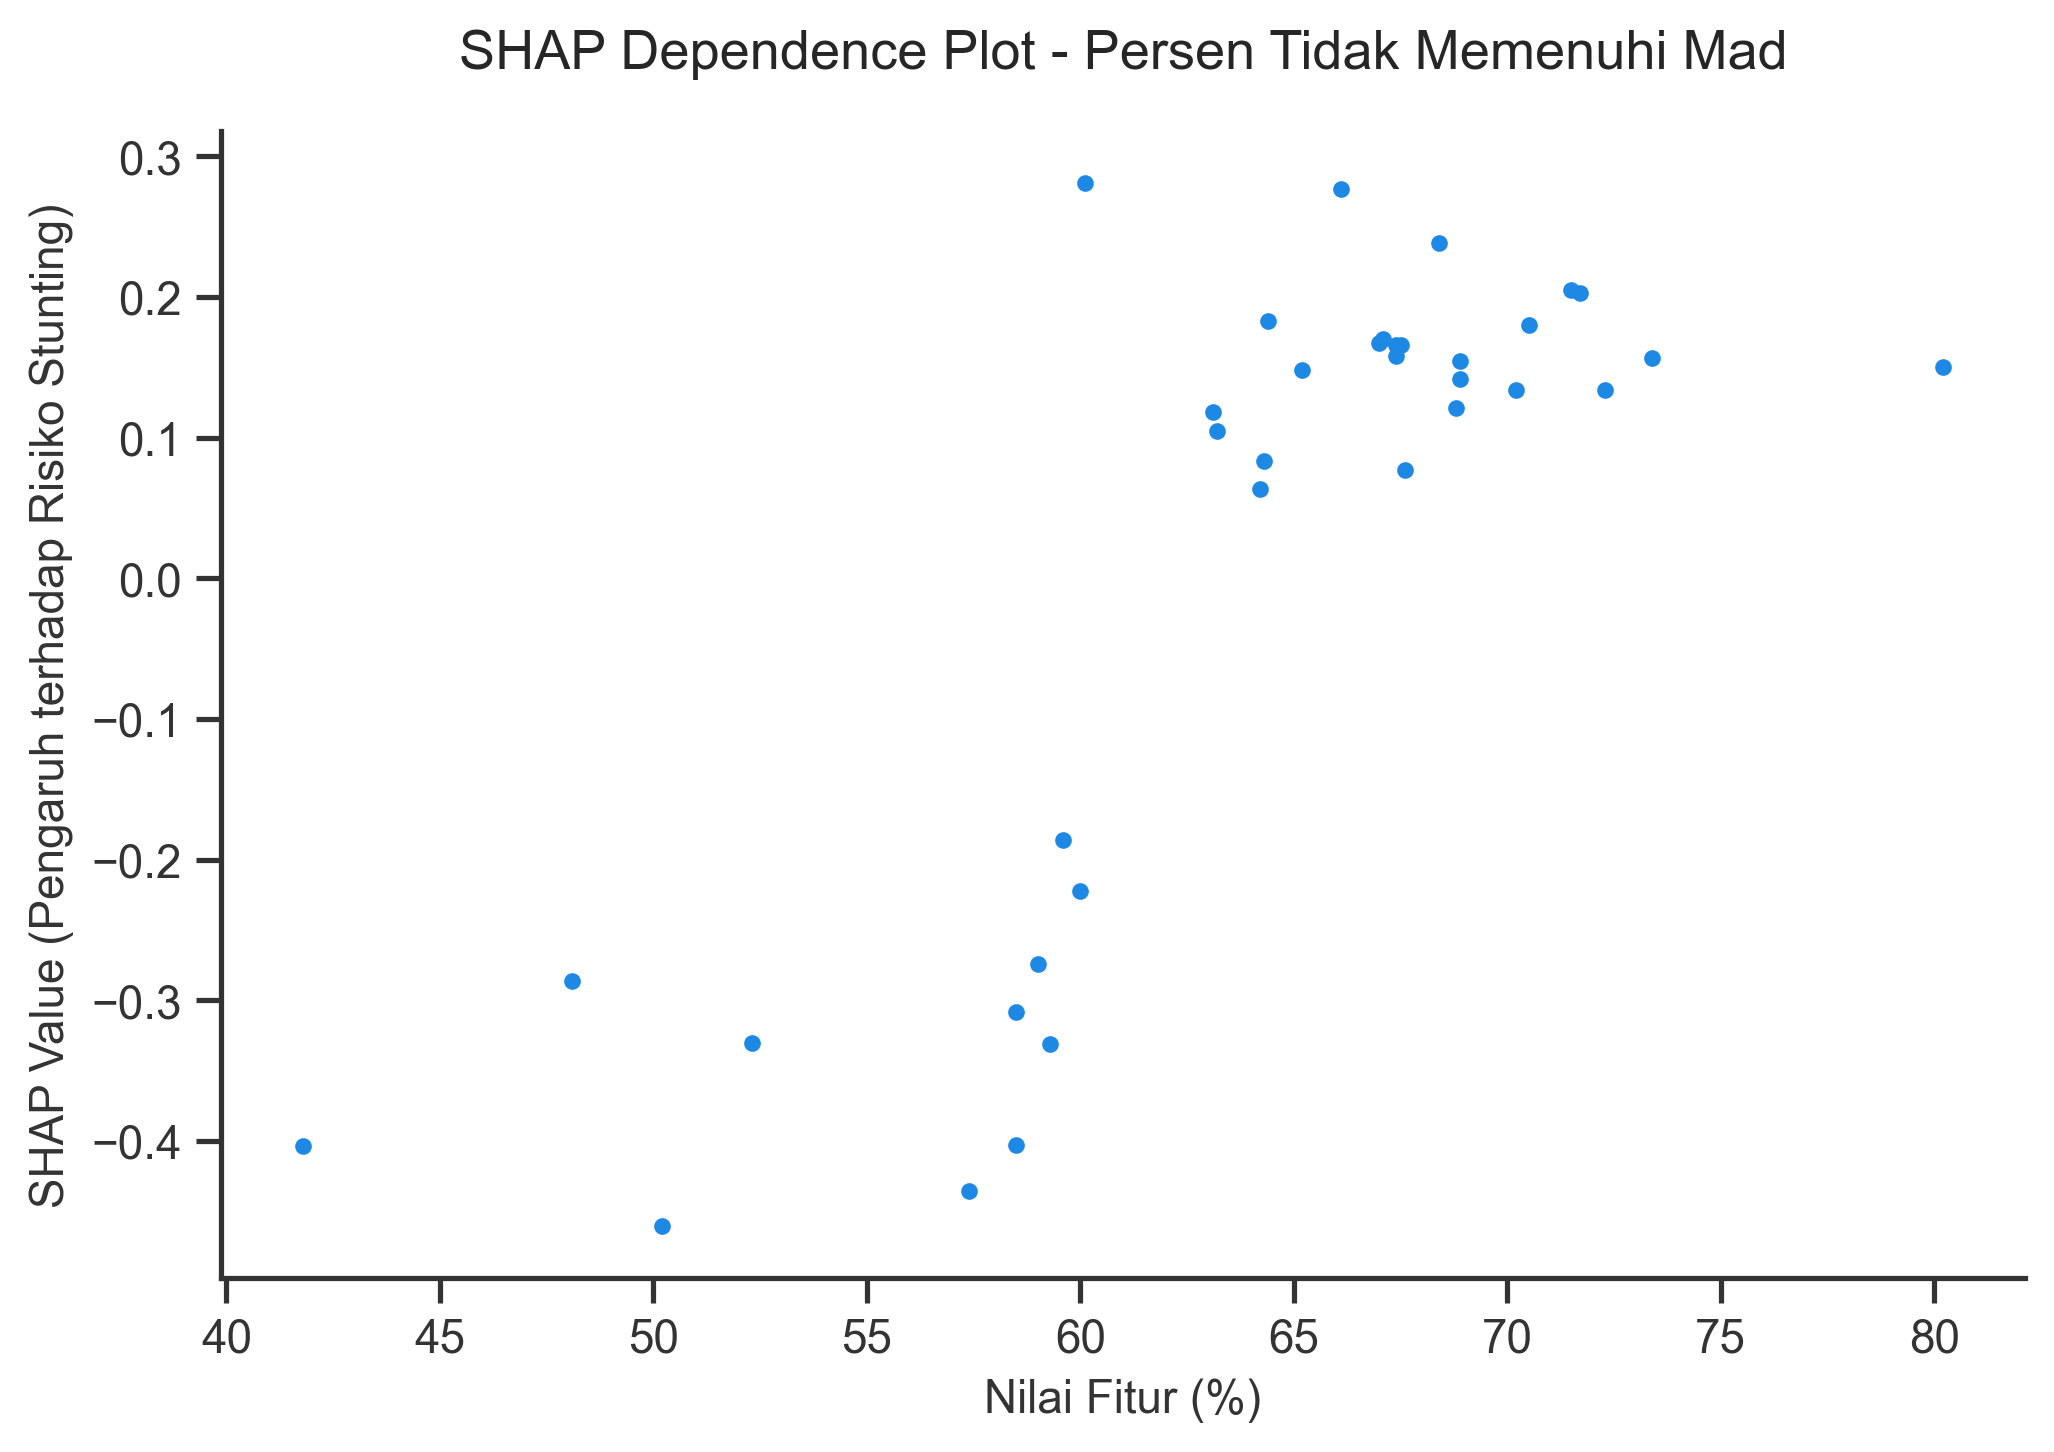
\includegraphics[width=0.48\textwidth]{figure/hasil_dependence_plot/dependence_persen_tidak_memenuhi_mad.png} \hfill
    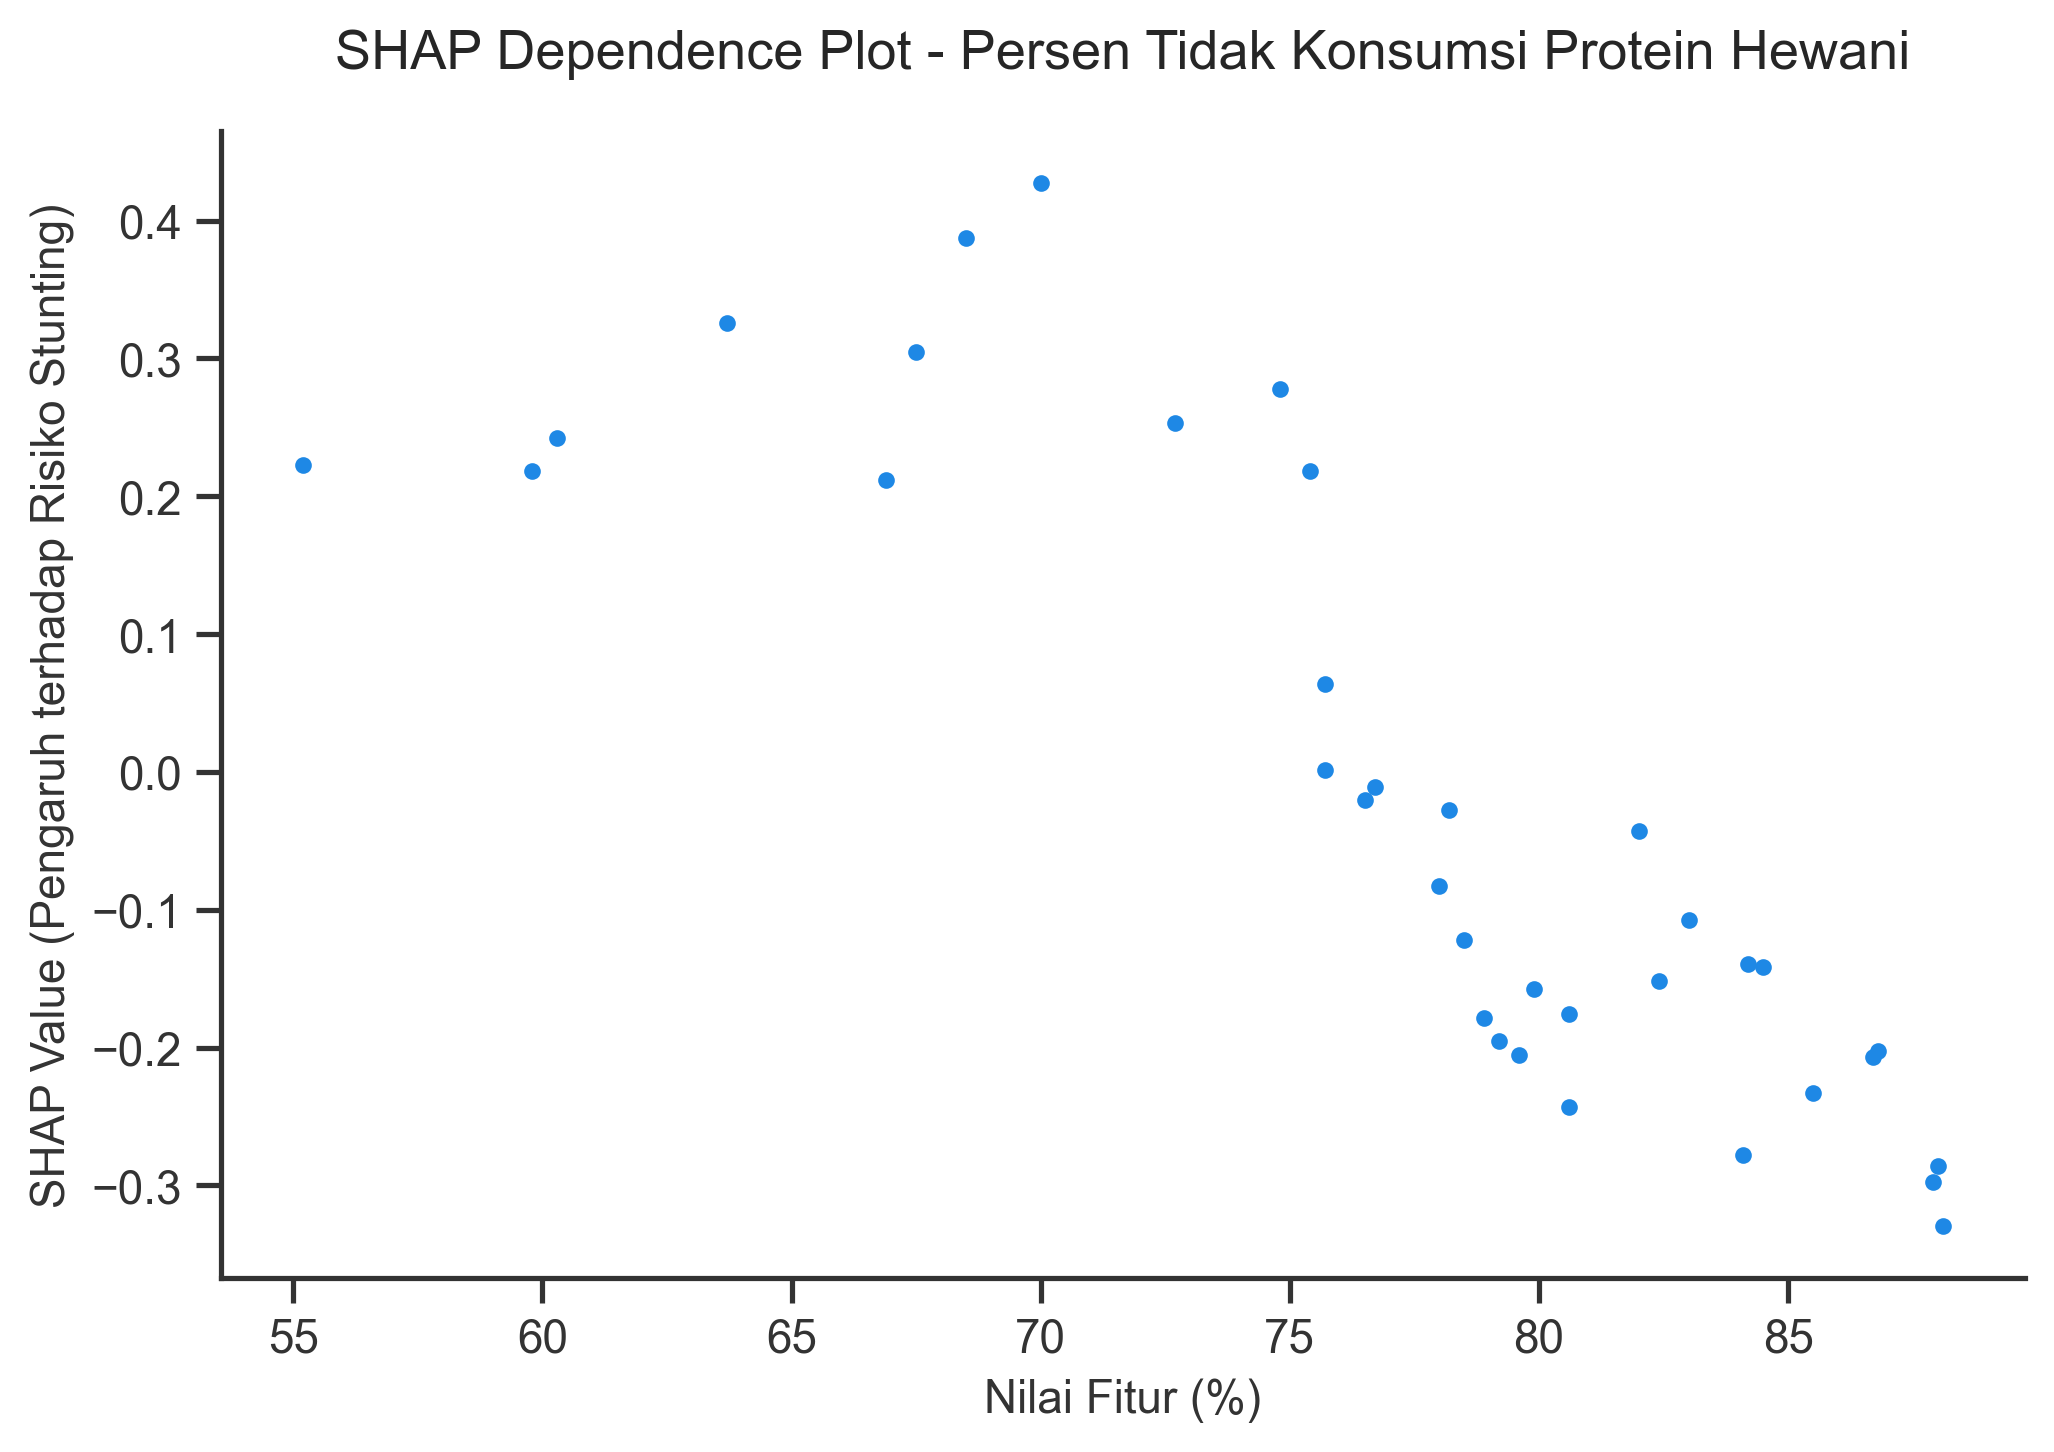
\includegraphics[width=0.48\textwidth]{figure/hasil_dependence_plot/dependence_persen_tidak_konsumsi_protein_hewani.png}
\end{figure}

\newpage
\begin{figure}[H]
    \centering
    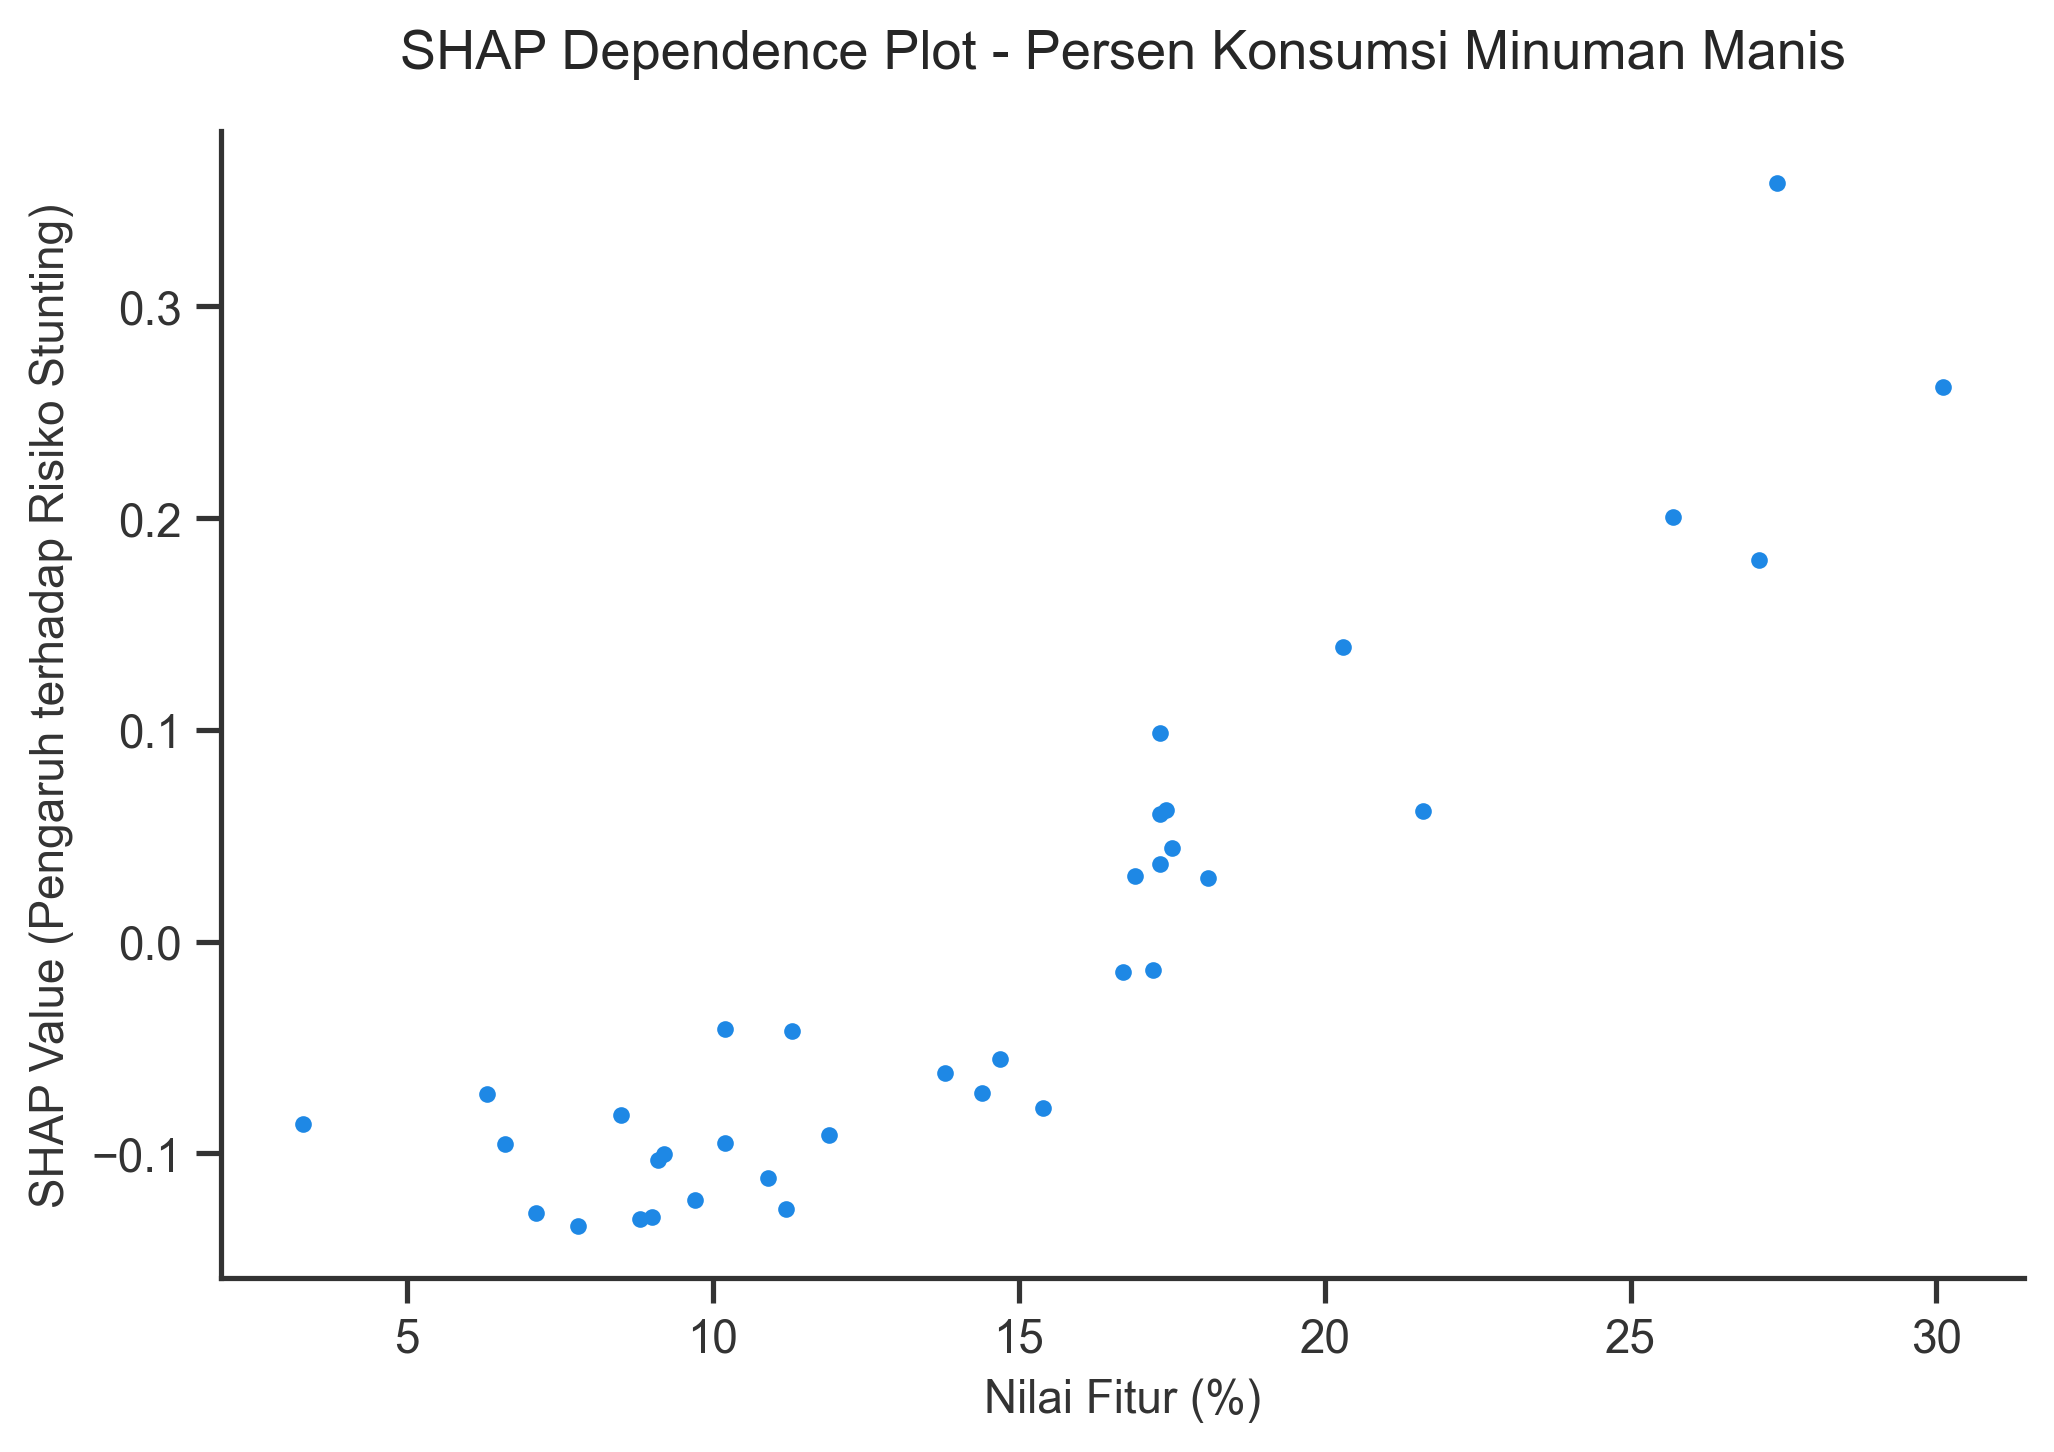
\includegraphics[width=0.48\textwidth]{figure/hasil_dependence_plot/dependence_persen_konsumsi_minuman_manis.png} \hfill
    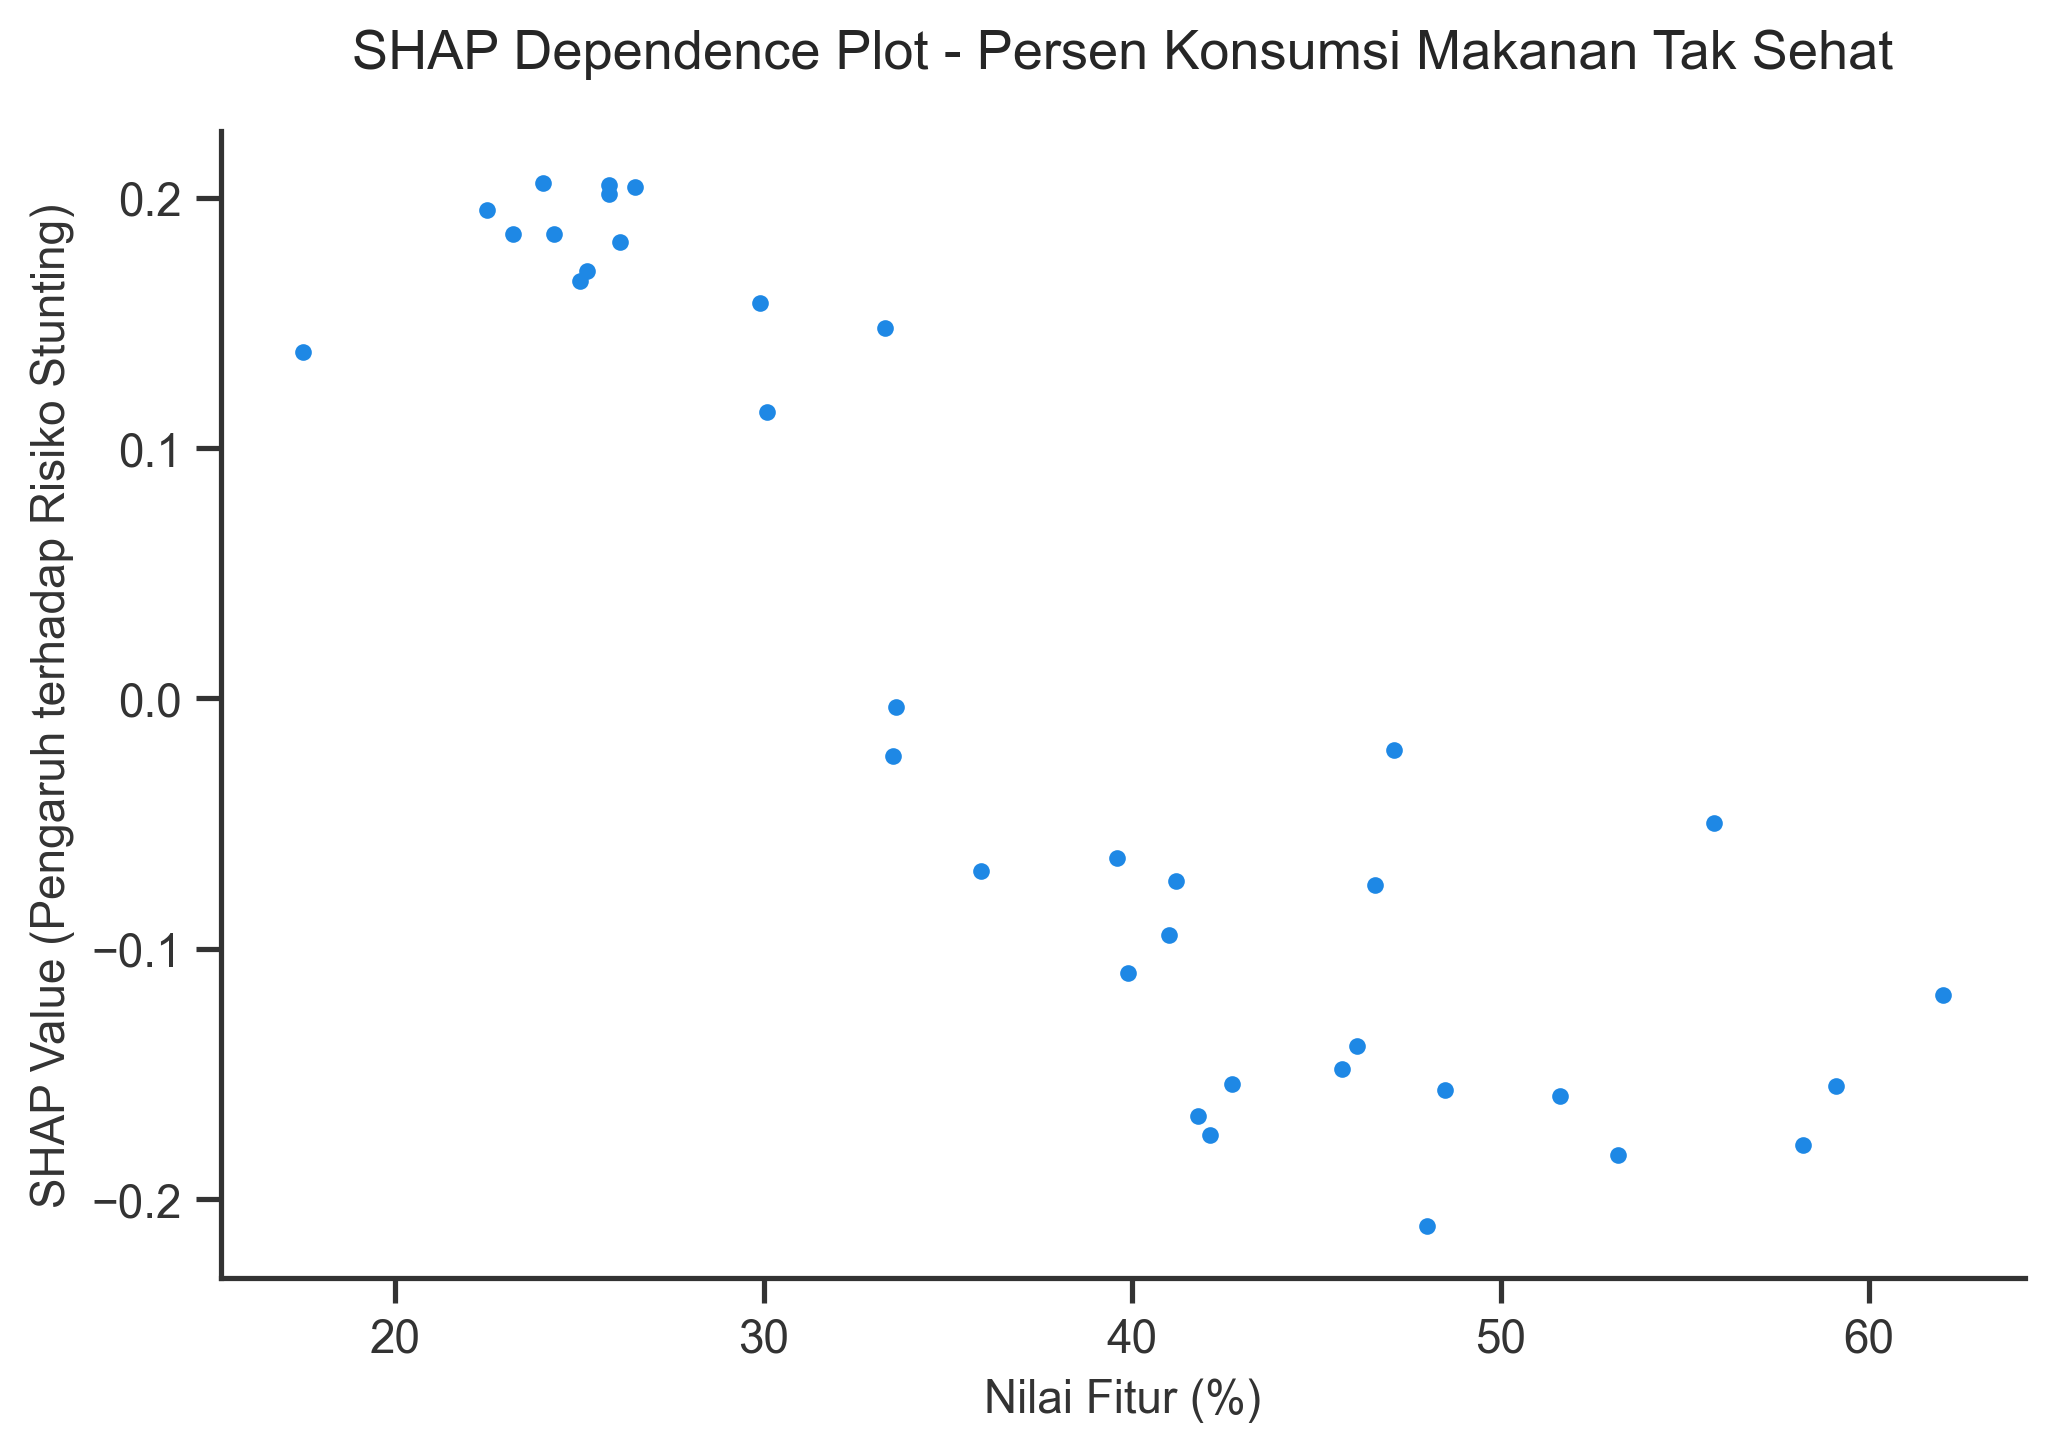
\includegraphics[width=0.48\textwidth]{figure/hasil_dependence_plot/dependence_persen_konsumsi_makanan_tak_sehat.png} \\ \vspace{0.2cm}
    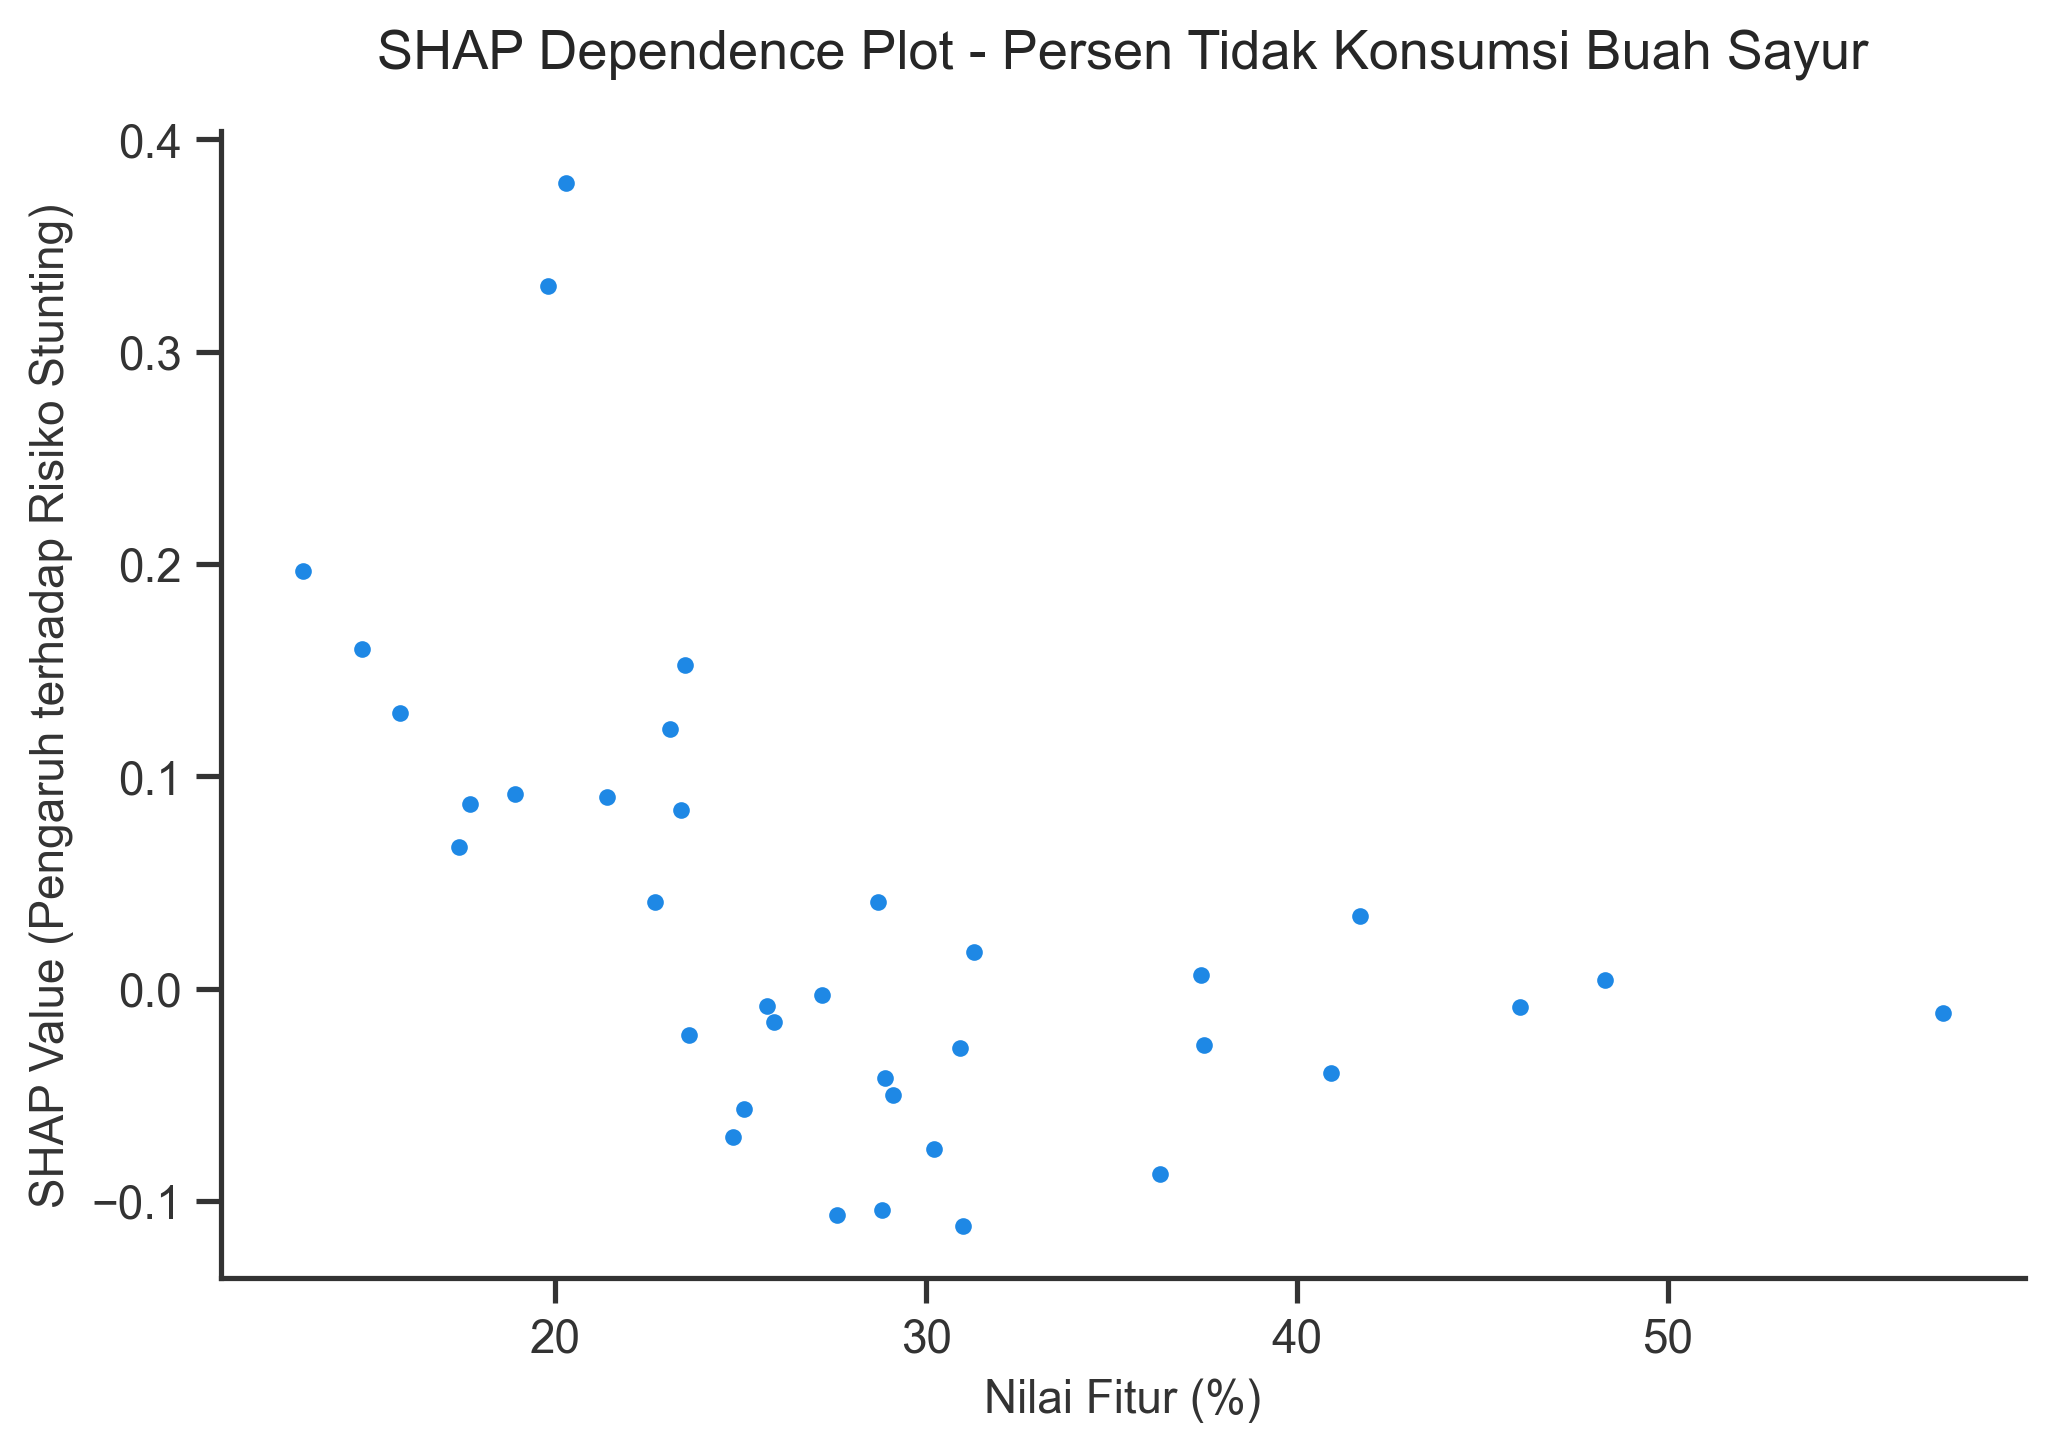
\includegraphics[width=0.48\textwidth]{figure/hasil_dependence_plot/dependence_persen_tidak_konsumsi_buah_sayur.png} \hfill
    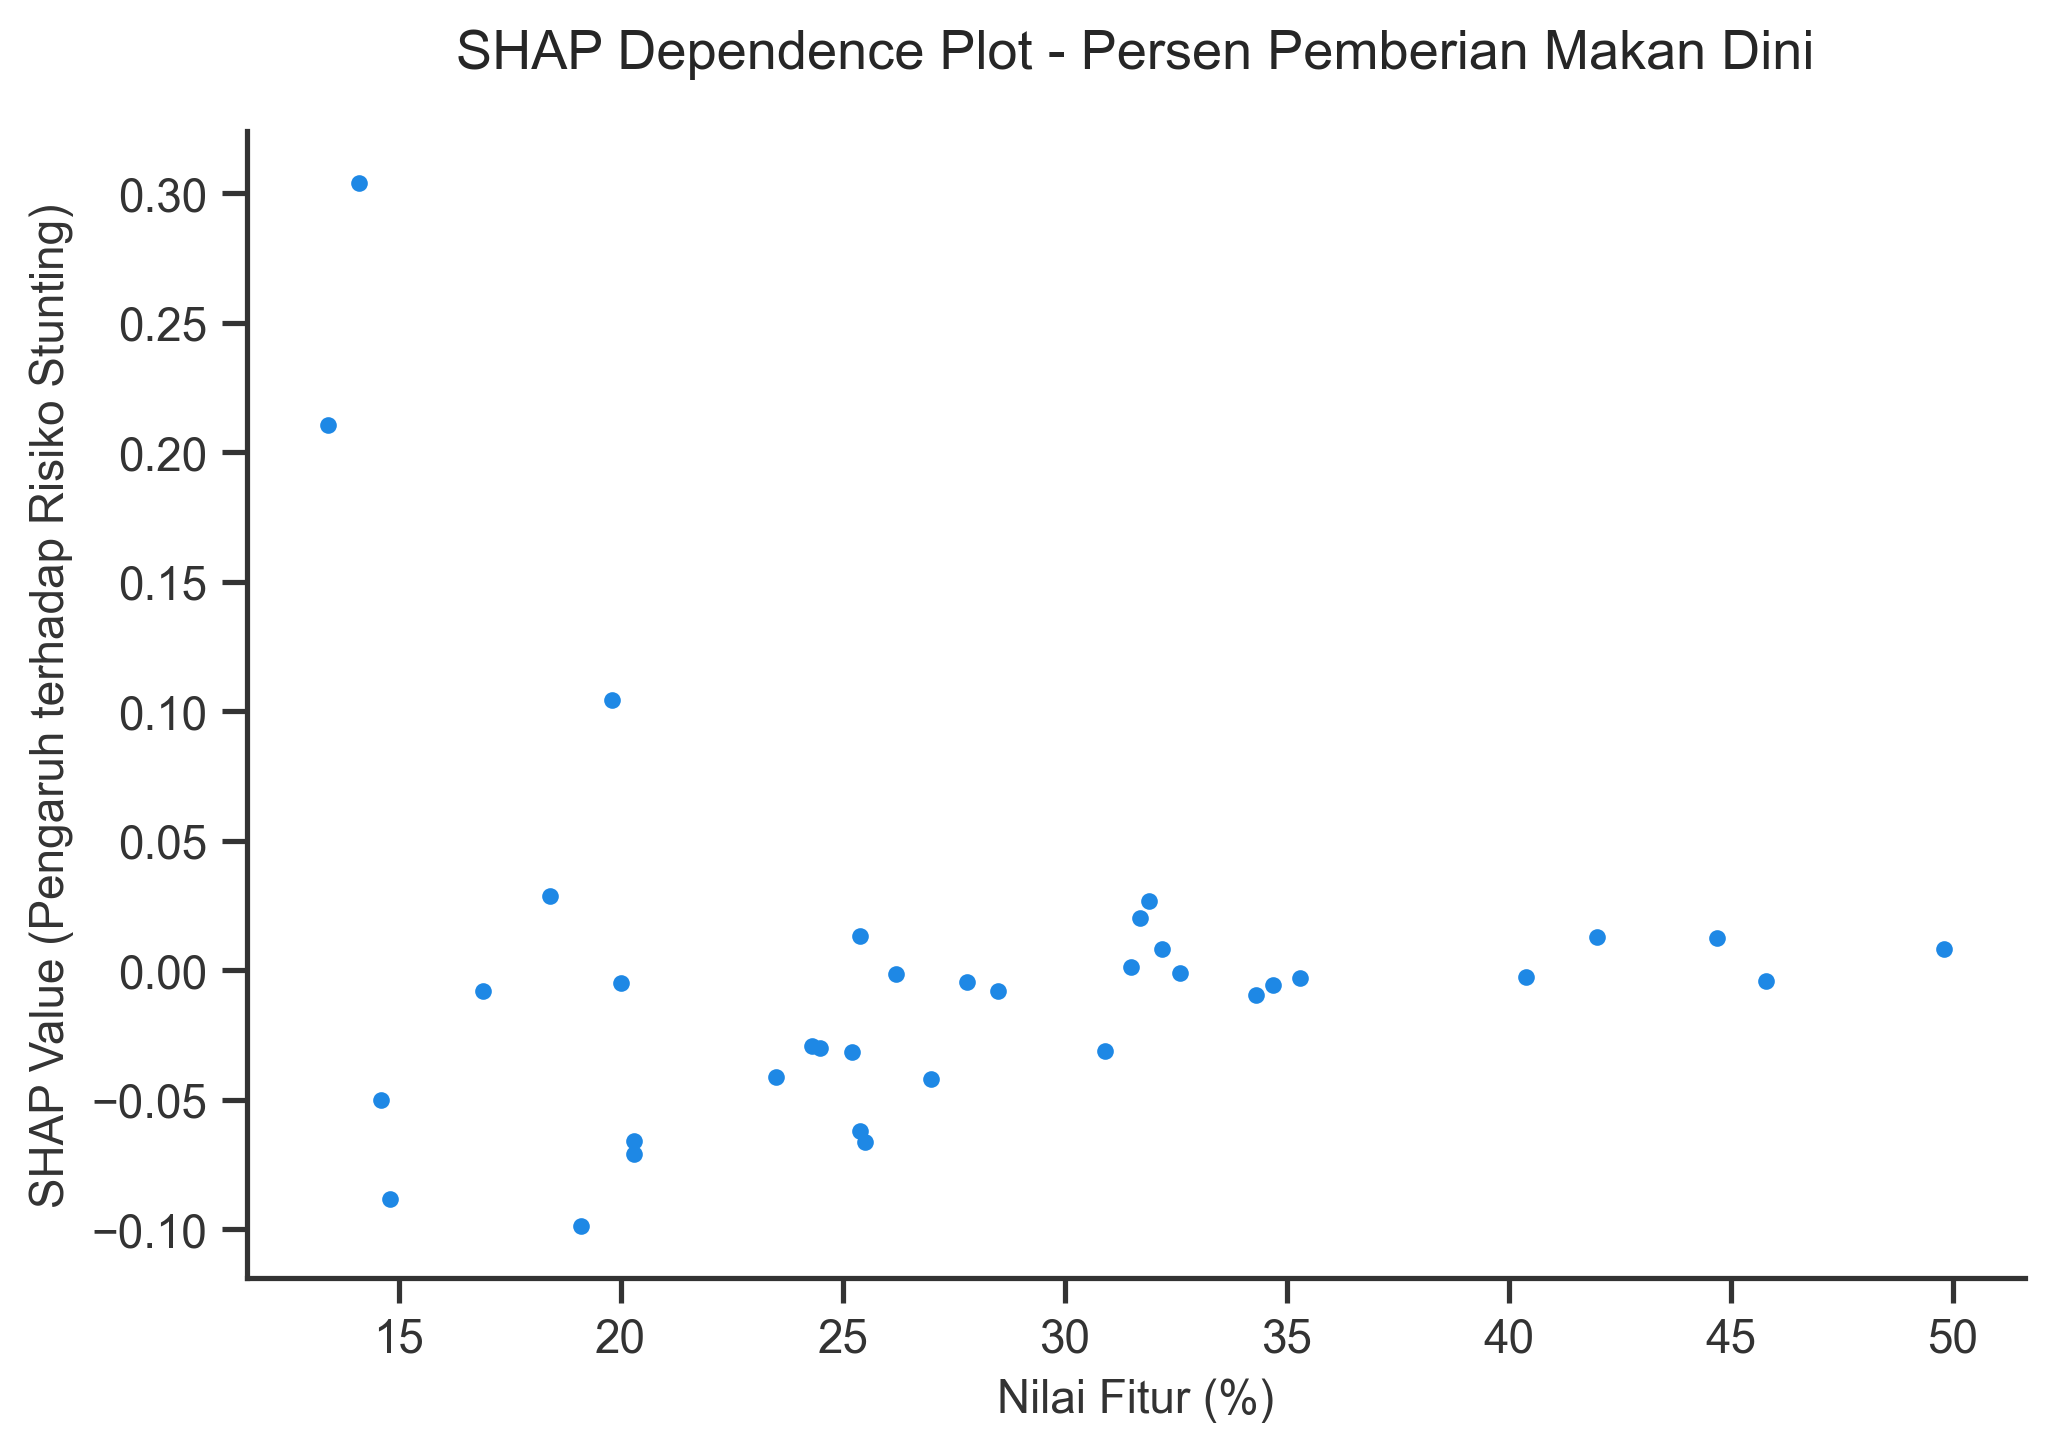
\includegraphics[width=0.48\textwidth]{figure/hasil_dependence_plot/dependence_persen_pemberian_makan_dini.png} \\ \vspace{0.2cm}
    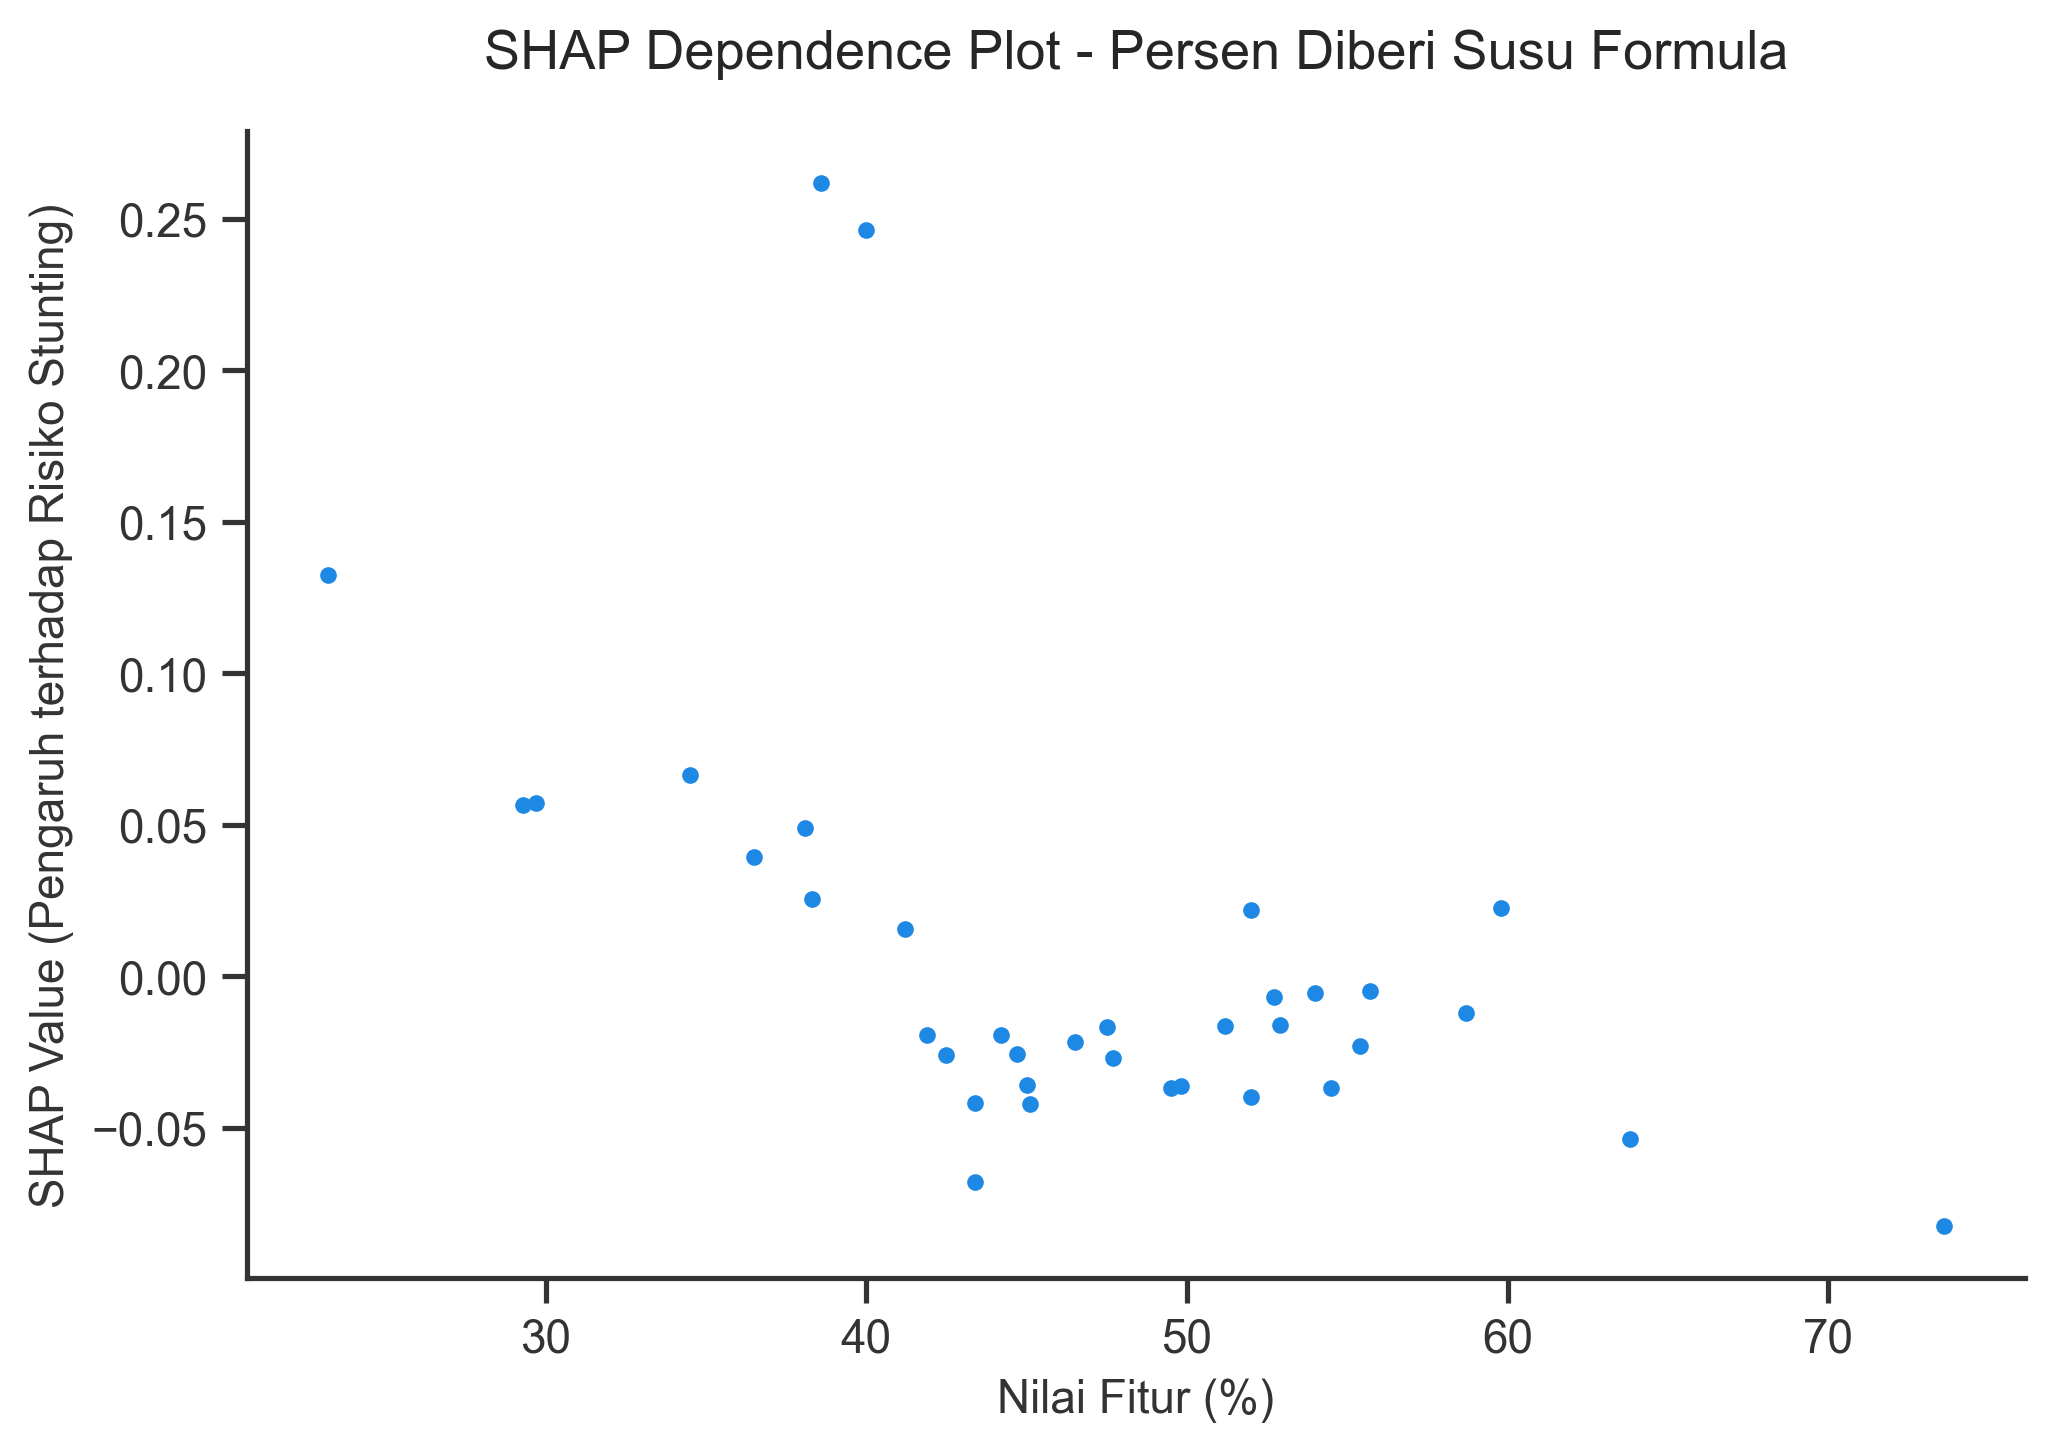
\includegraphics[width=0.48\textwidth]{figure/hasil_dependence_plot/dependence_persen_diberi_susu_formula.png} \hfill
    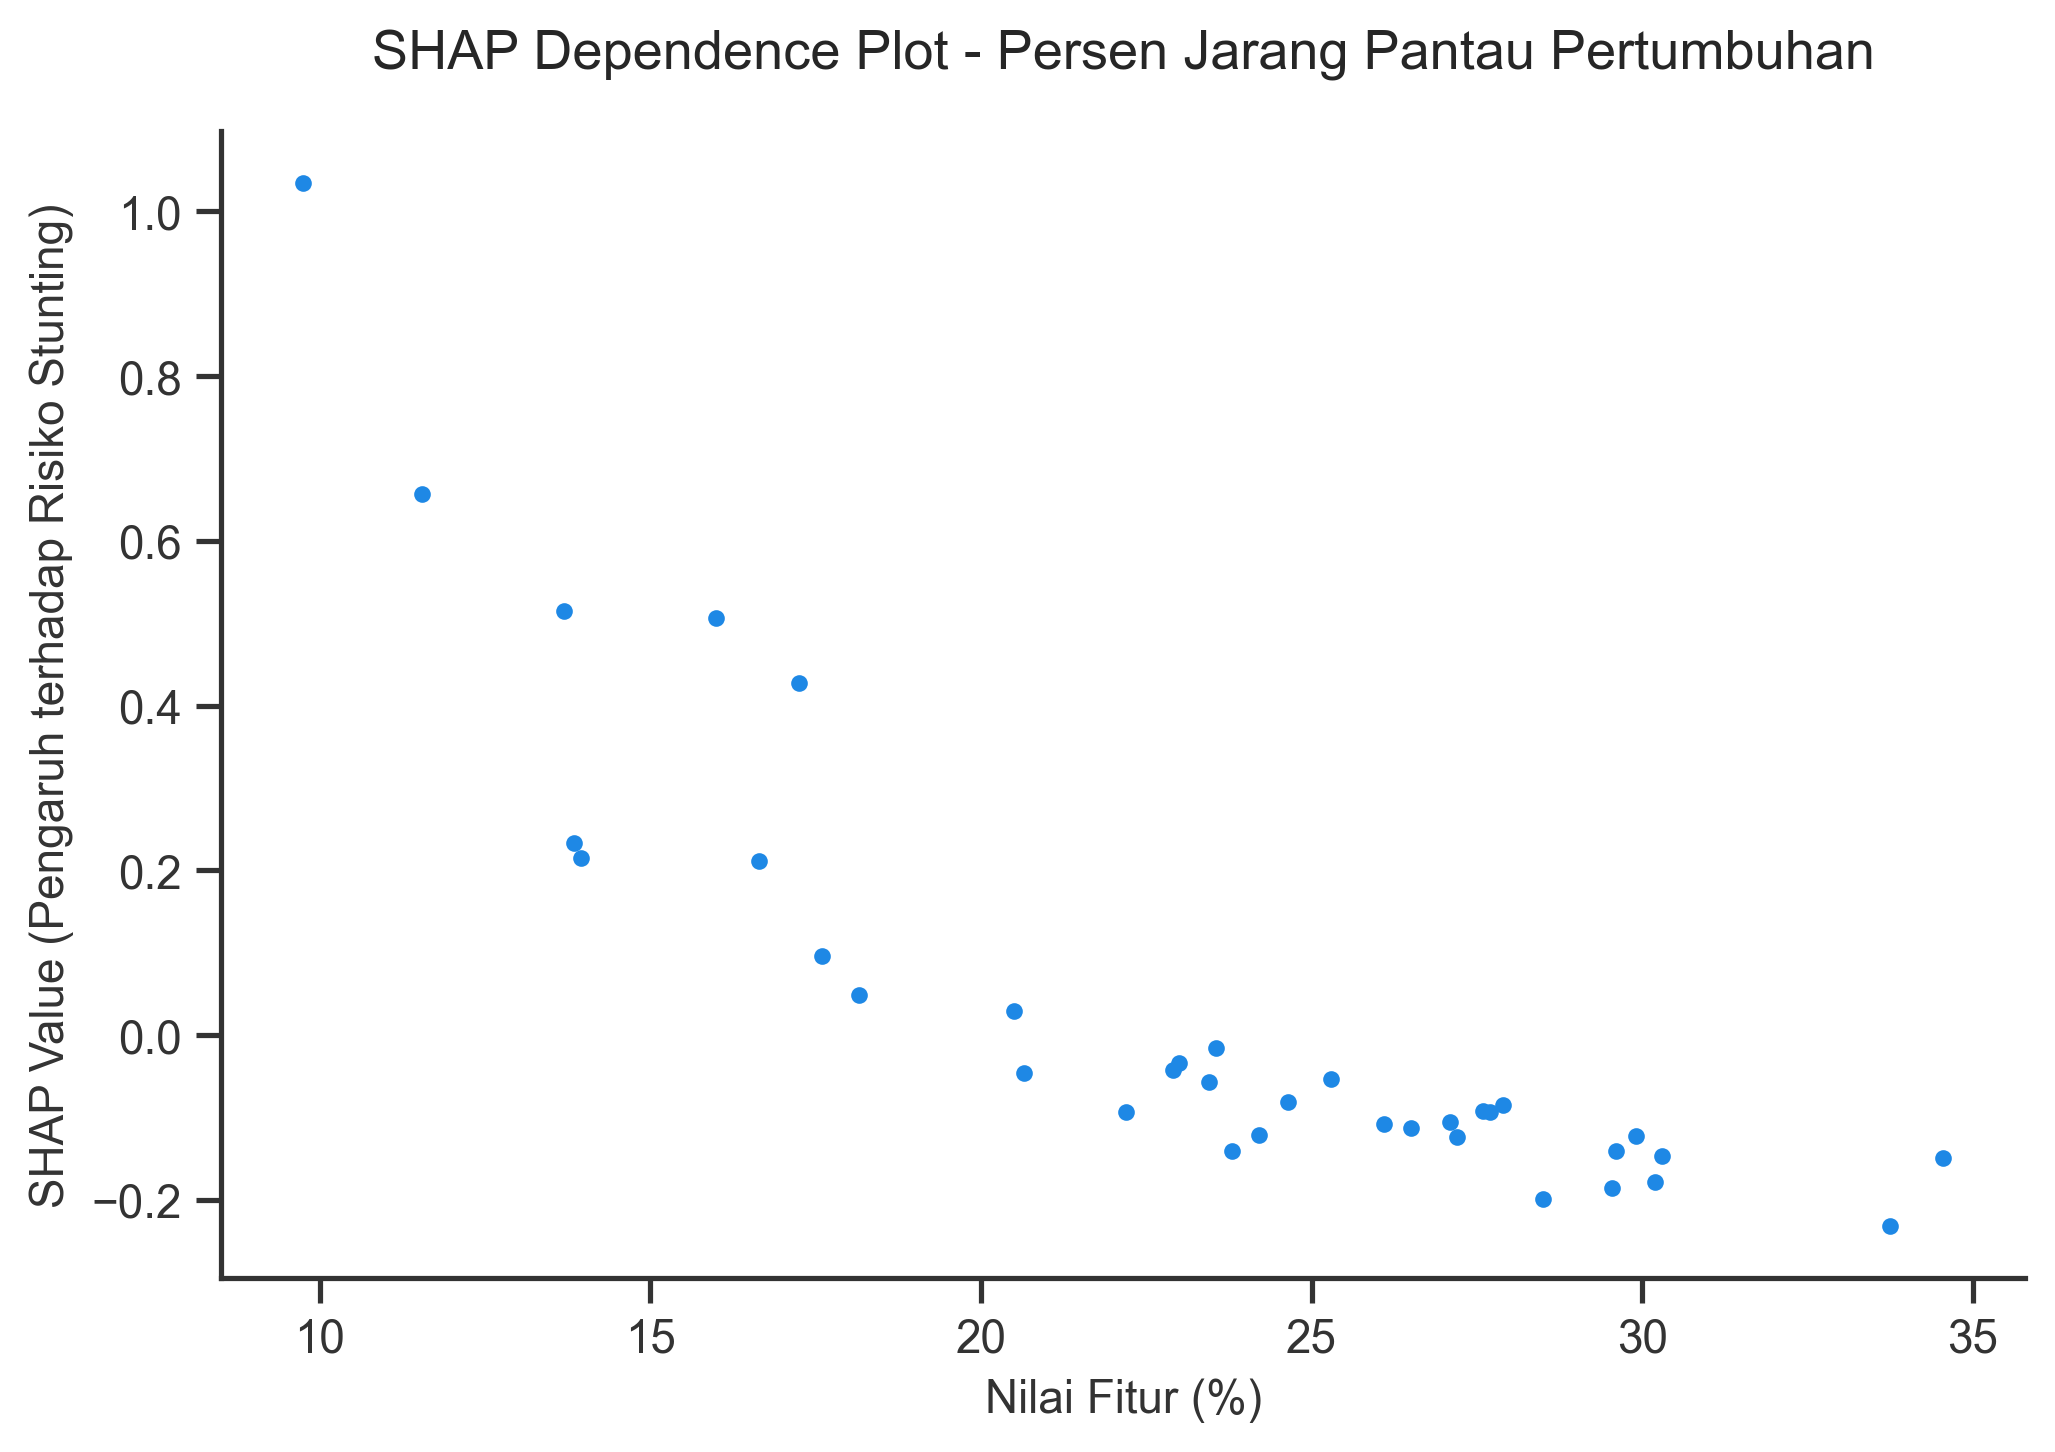
\includegraphics[width=0.48\textwidth]{figure/hasil_dependence_plot/dependence_persen_jarang_pantau_pertumbuhan.png} \\ \vspace{0.2cm}
    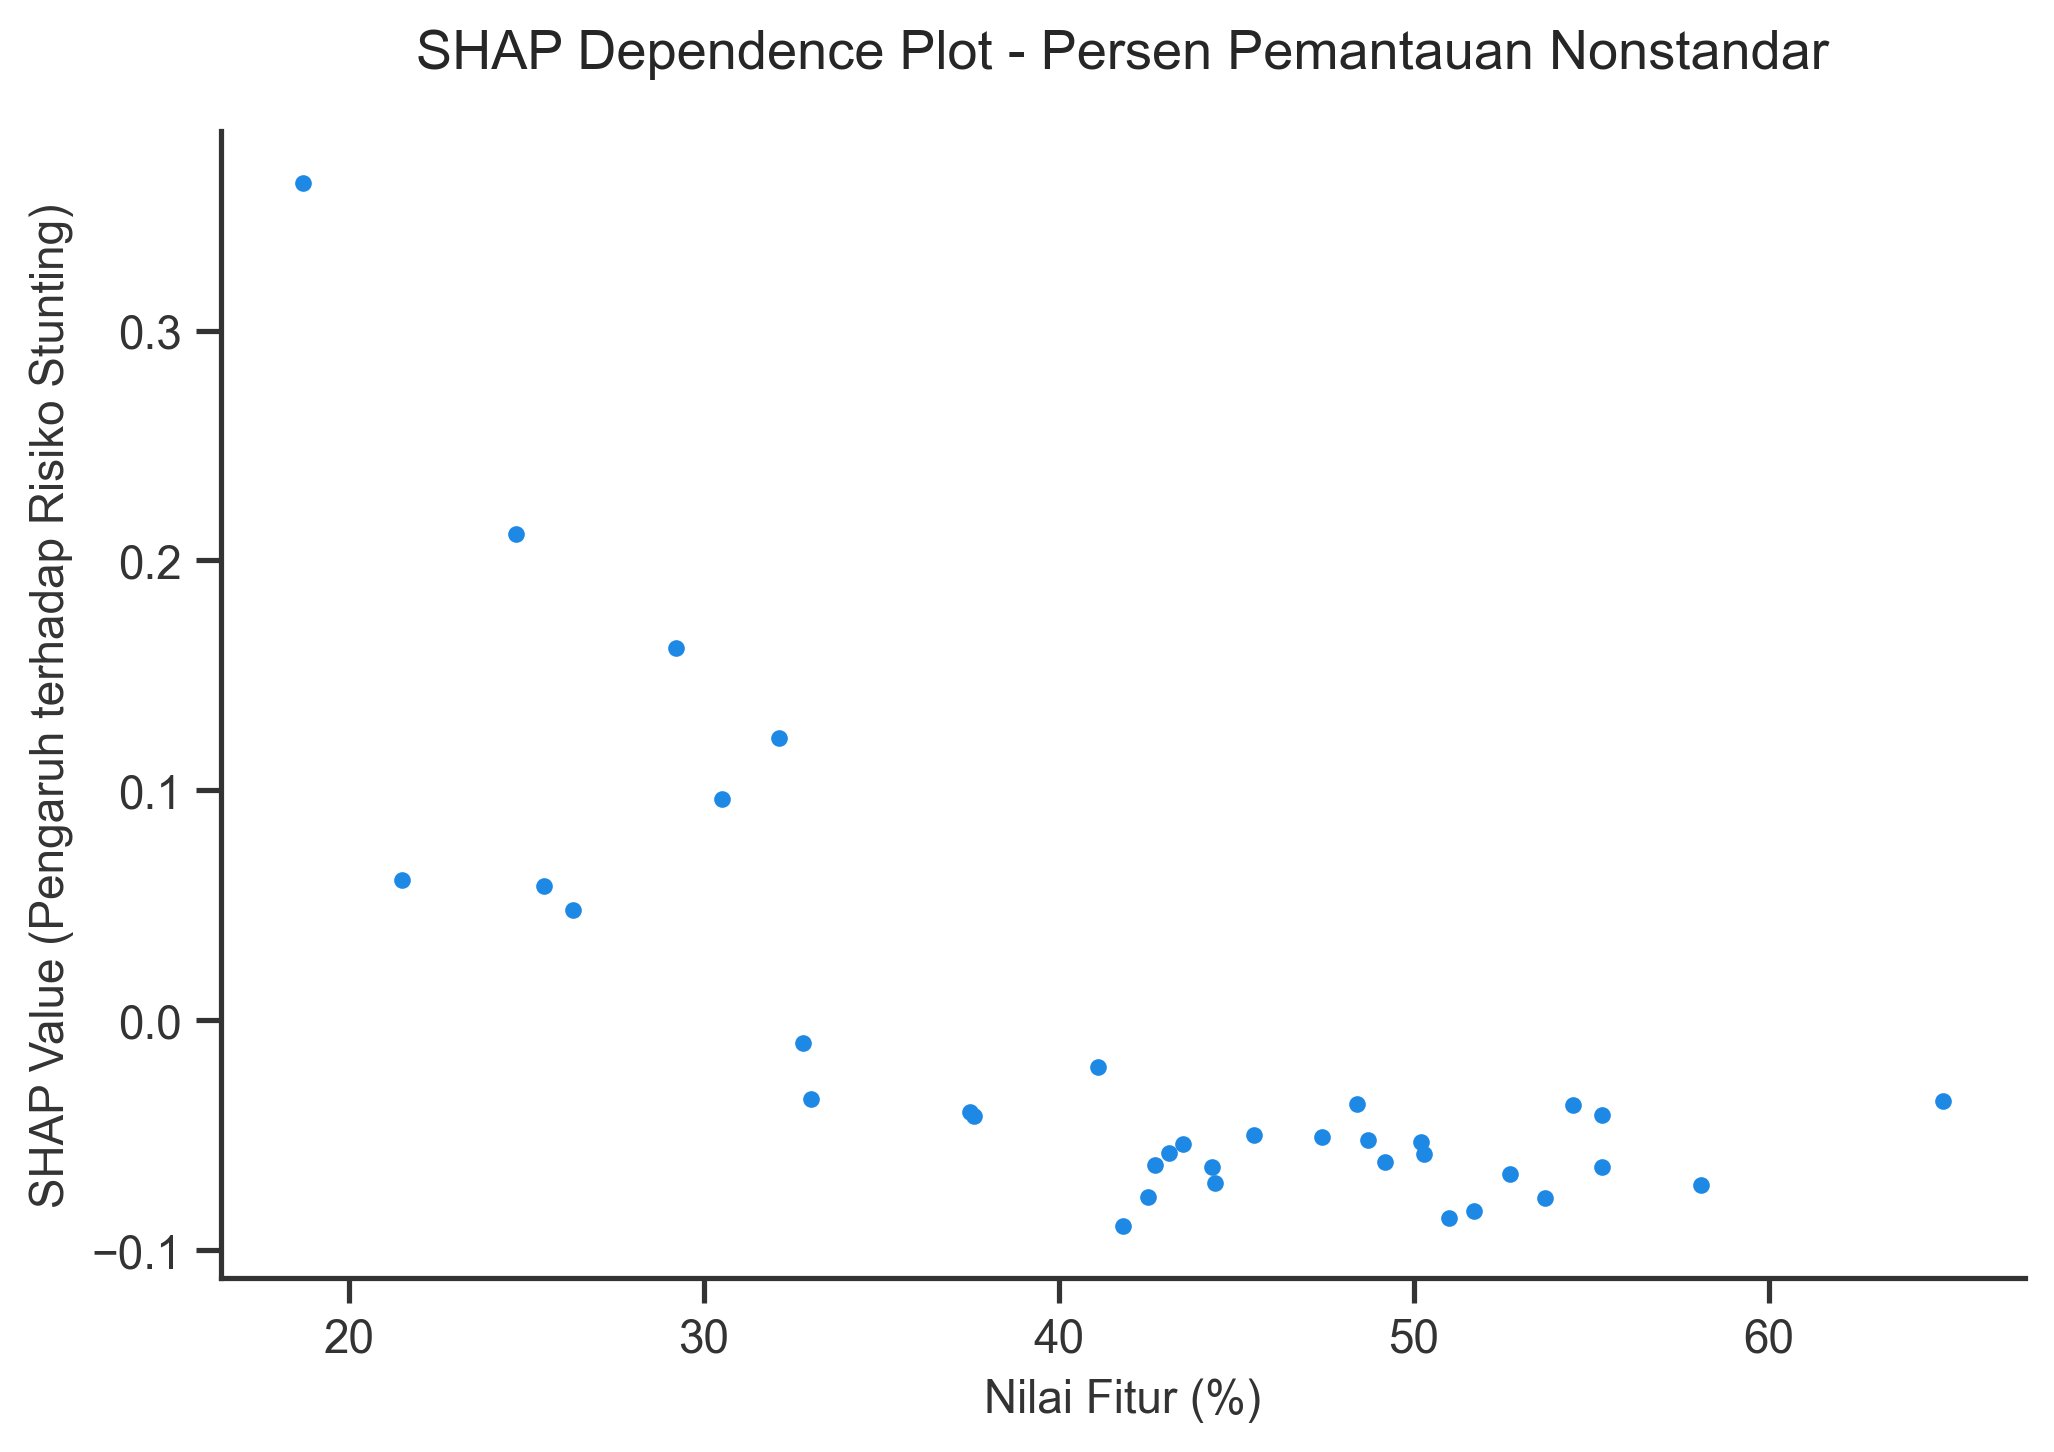
\includegraphics[width=0.48\textwidth]{figure/hasil_dependence_plot/dependence_persen_pemantauan_nonstandar.png} \hfill
    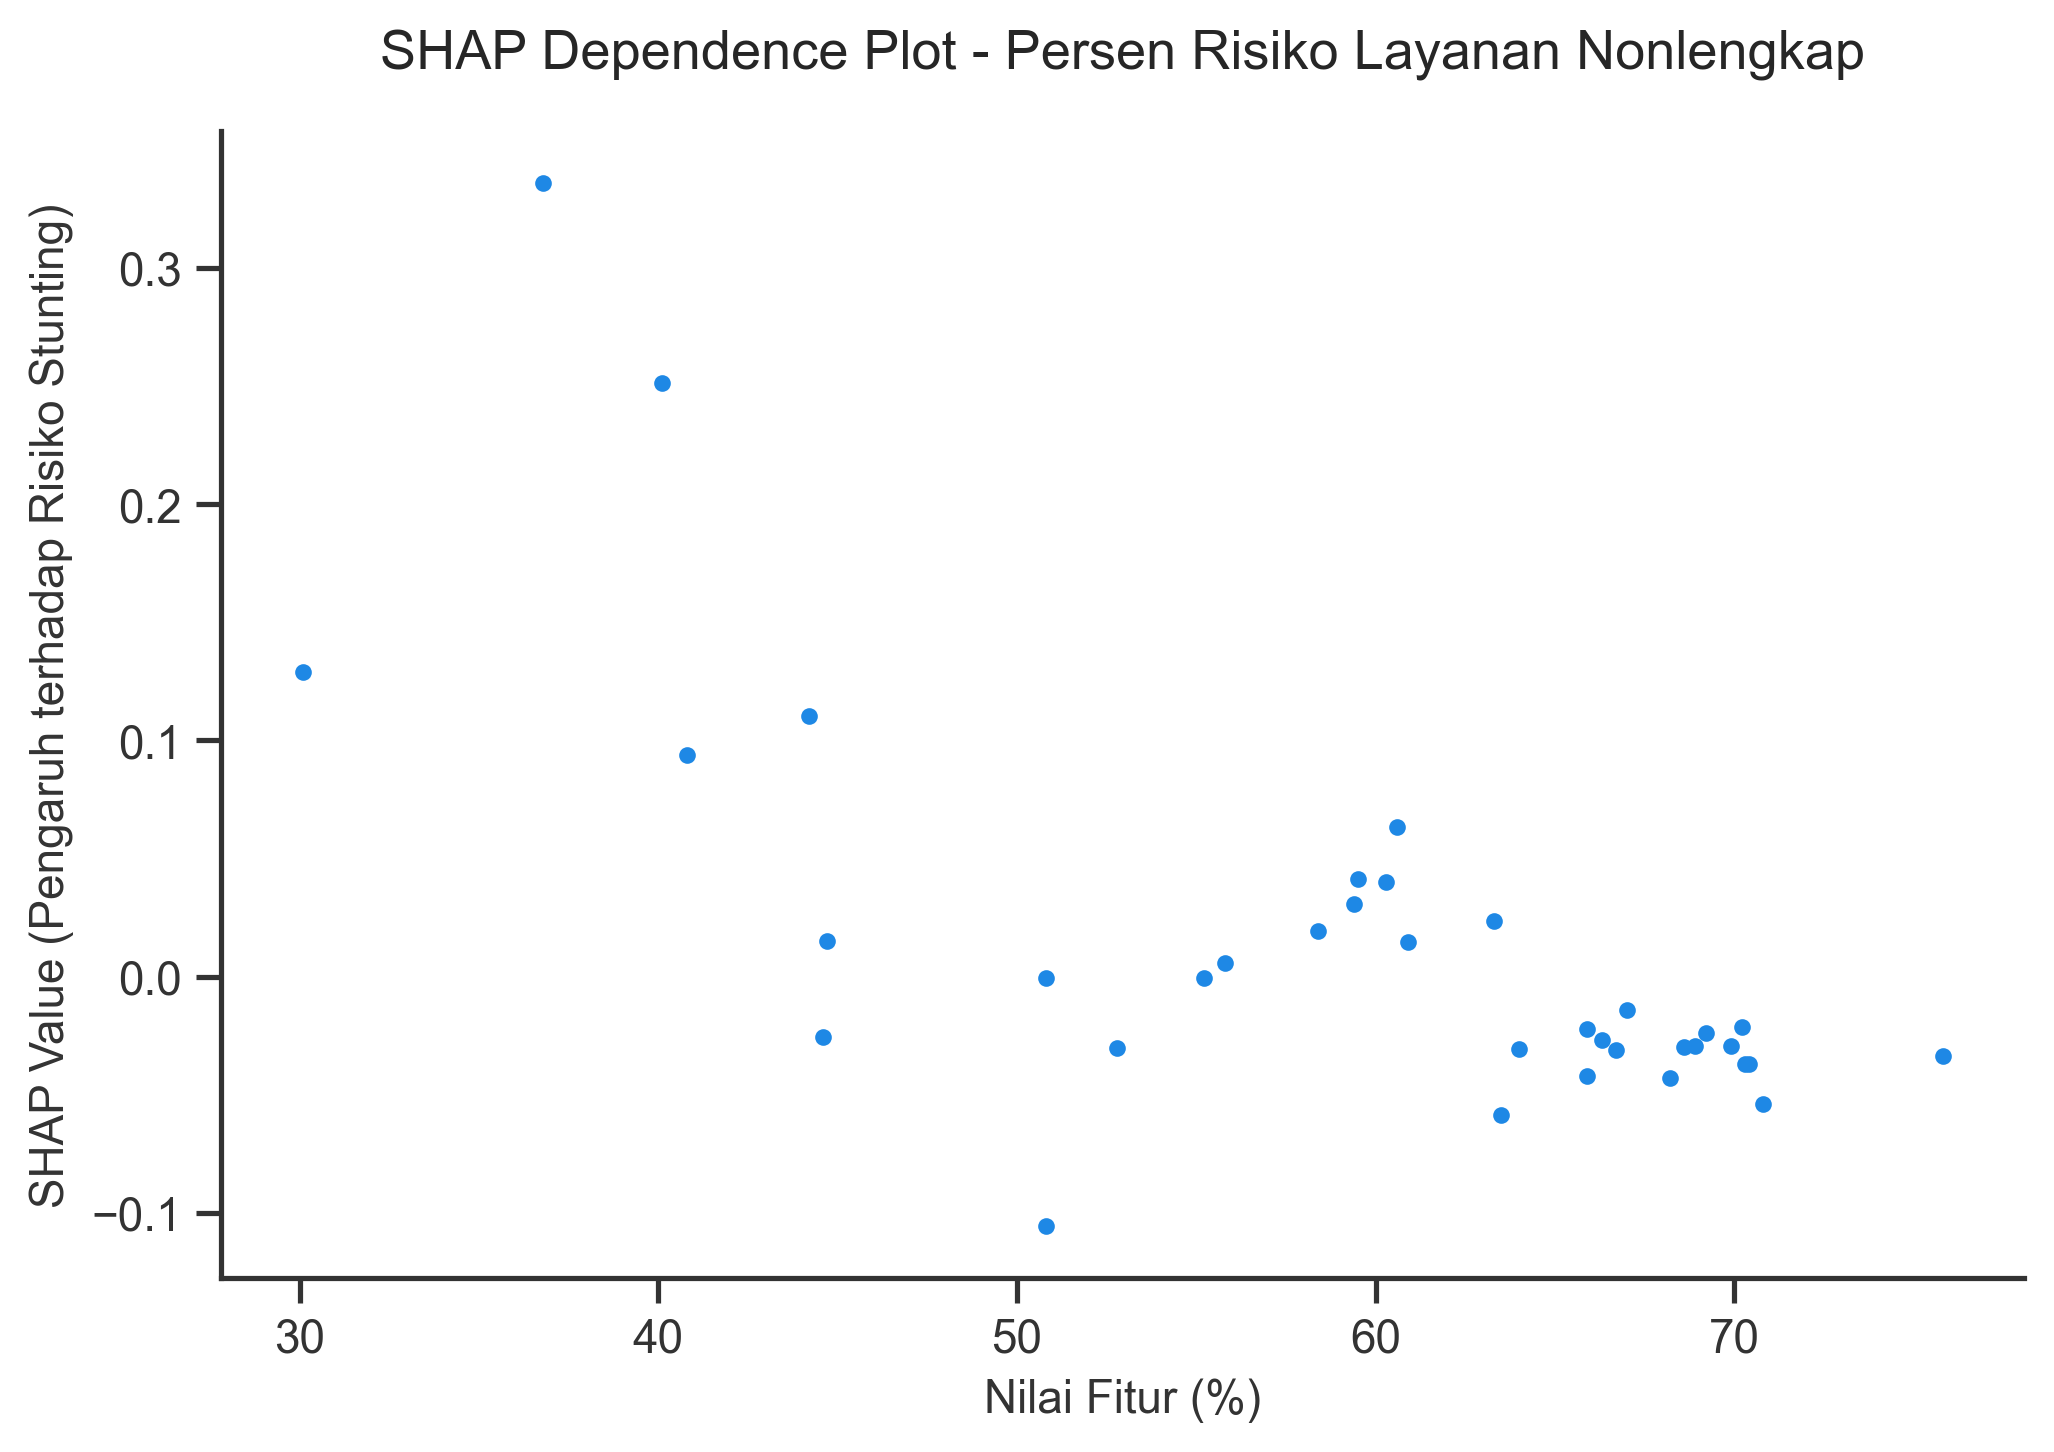
\includegraphics[width=0.48\textwidth]{figure/hasil_dependence_plot/dependence_persen_risiko_layanan_nonlengkap.png}
\end{figure}

\newpage
\begin{figure}[H]
    \centering
    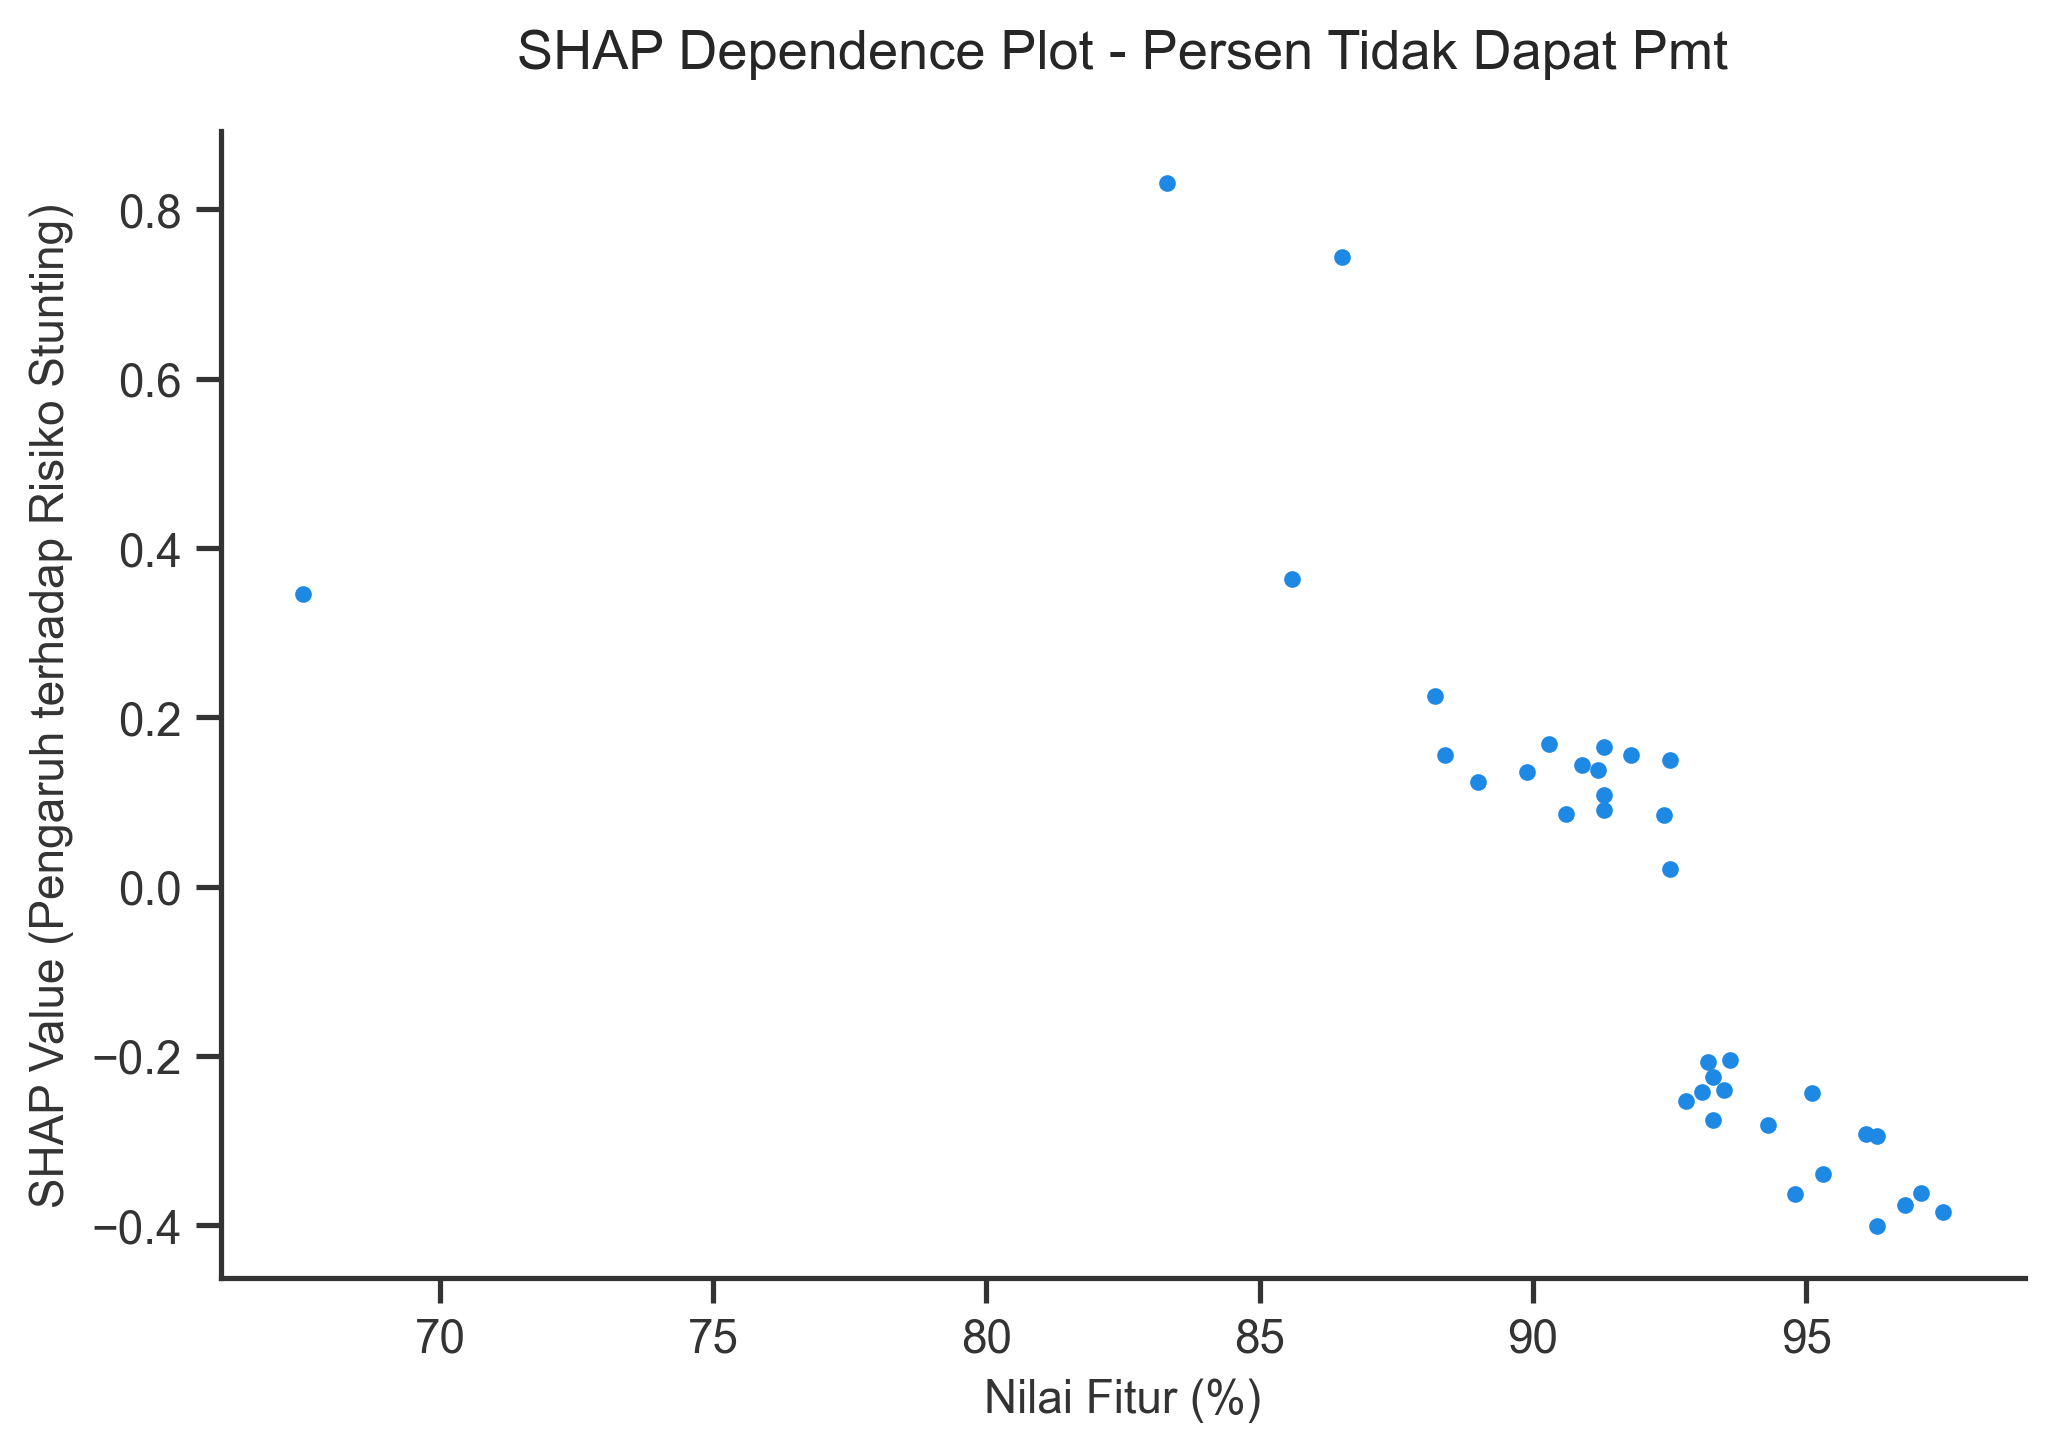
\includegraphics[width=0.48\textwidth]{figure/hasil_dependence_plot/dependence_persen_tidak_dapat_pmt.png} \hfill
    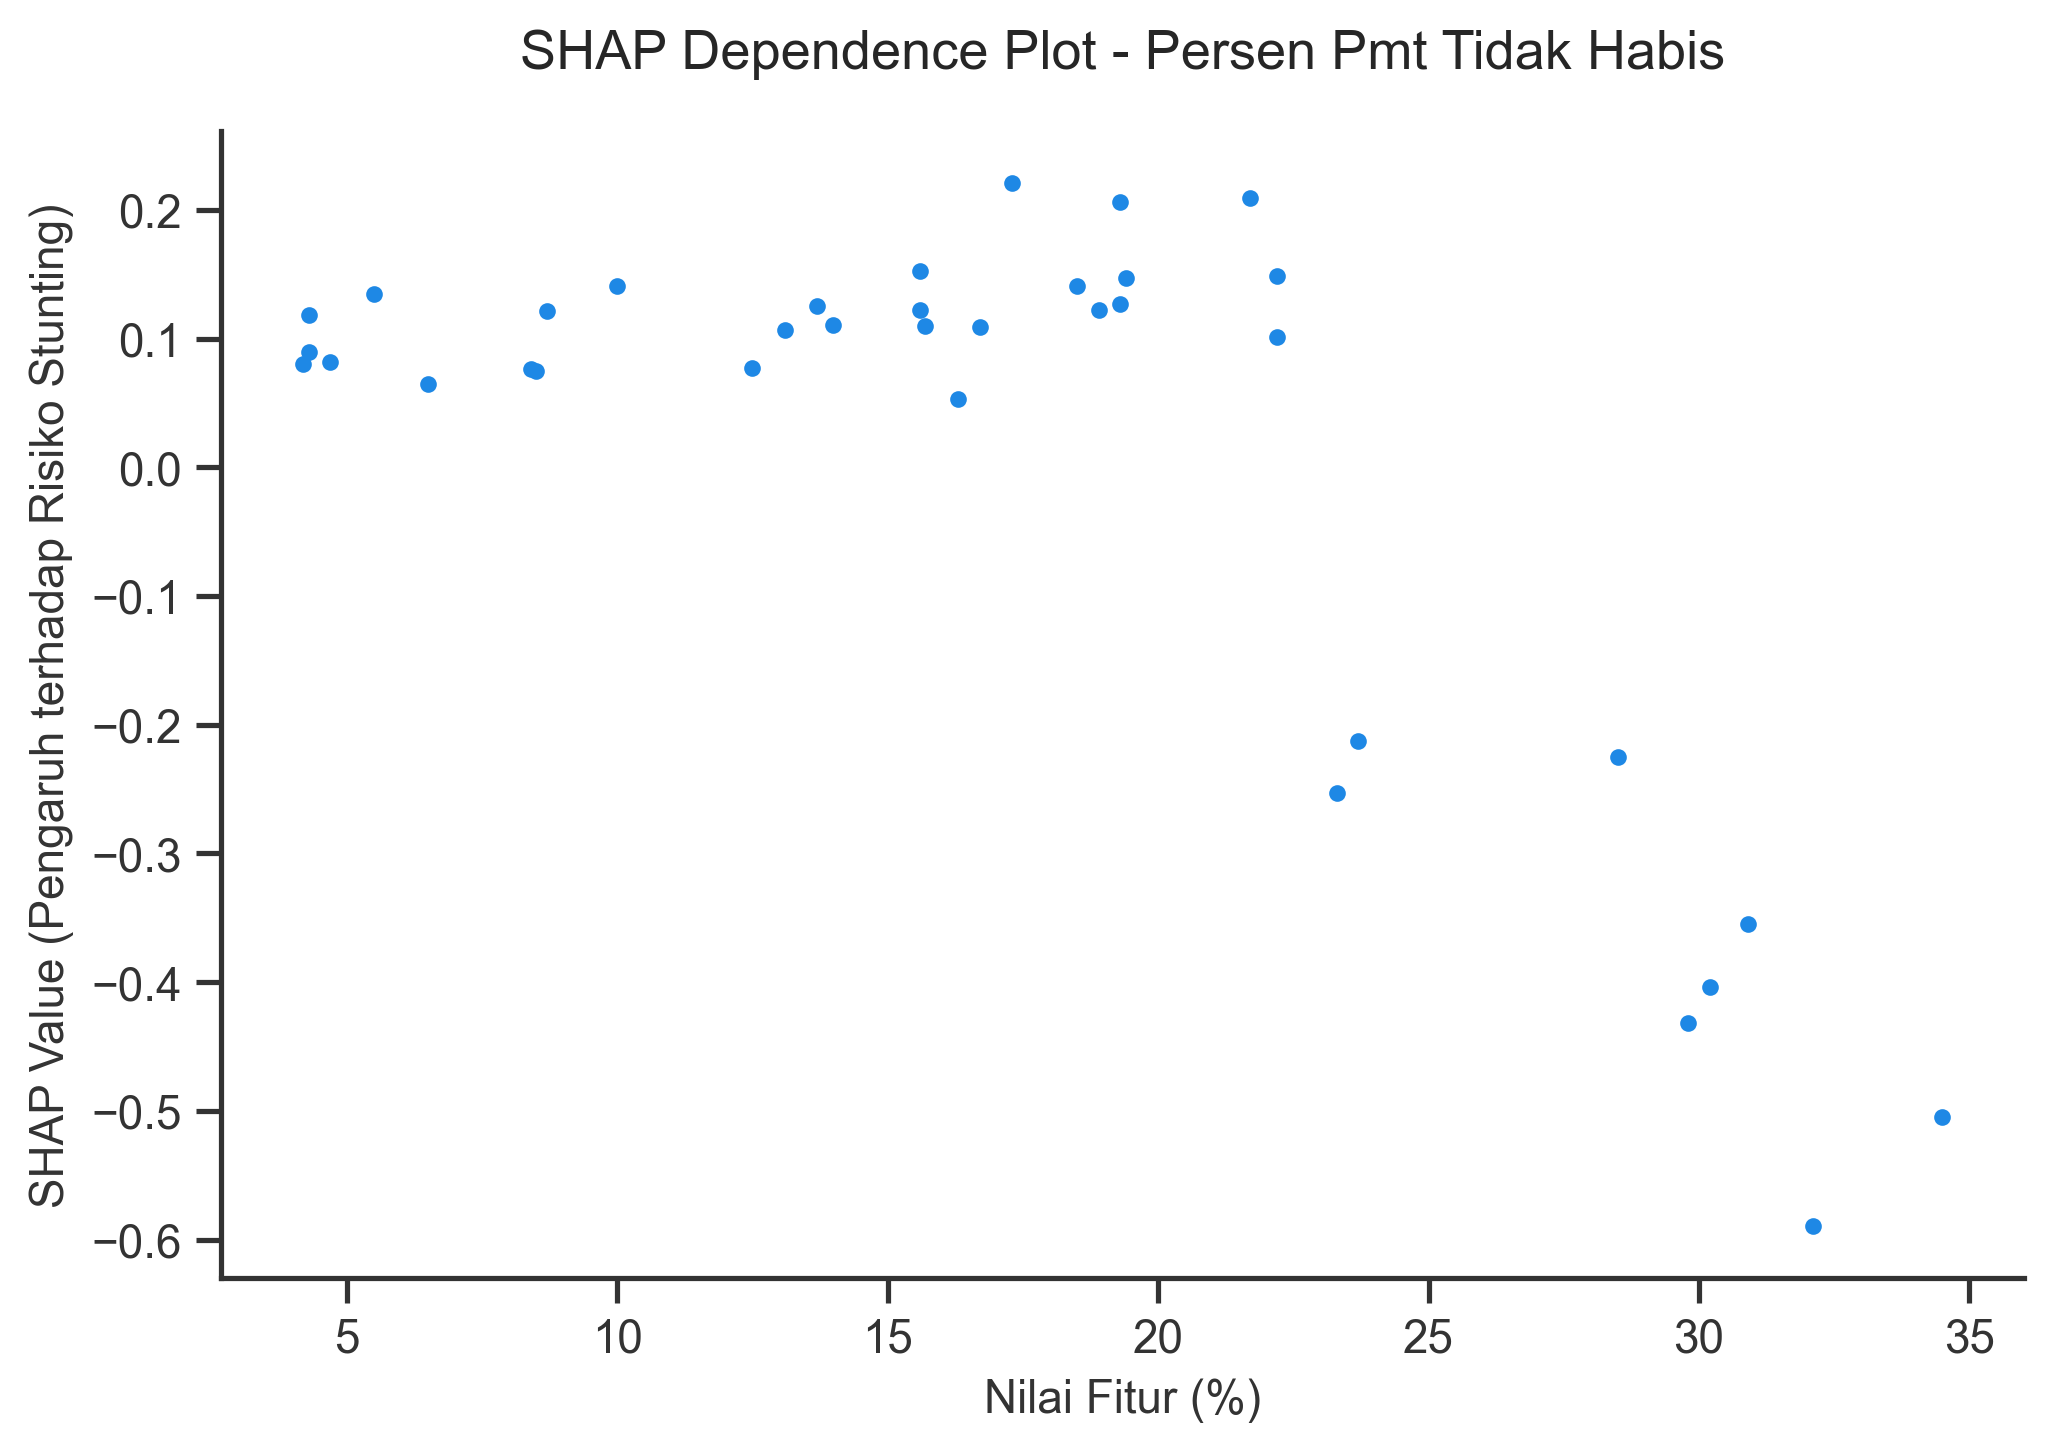
\includegraphics[width=0.48\textwidth]{figure/hasil_dependence_plot/dependence_persen_pmt_tidak_habis.png} \\ \vspace{0.2cm}
    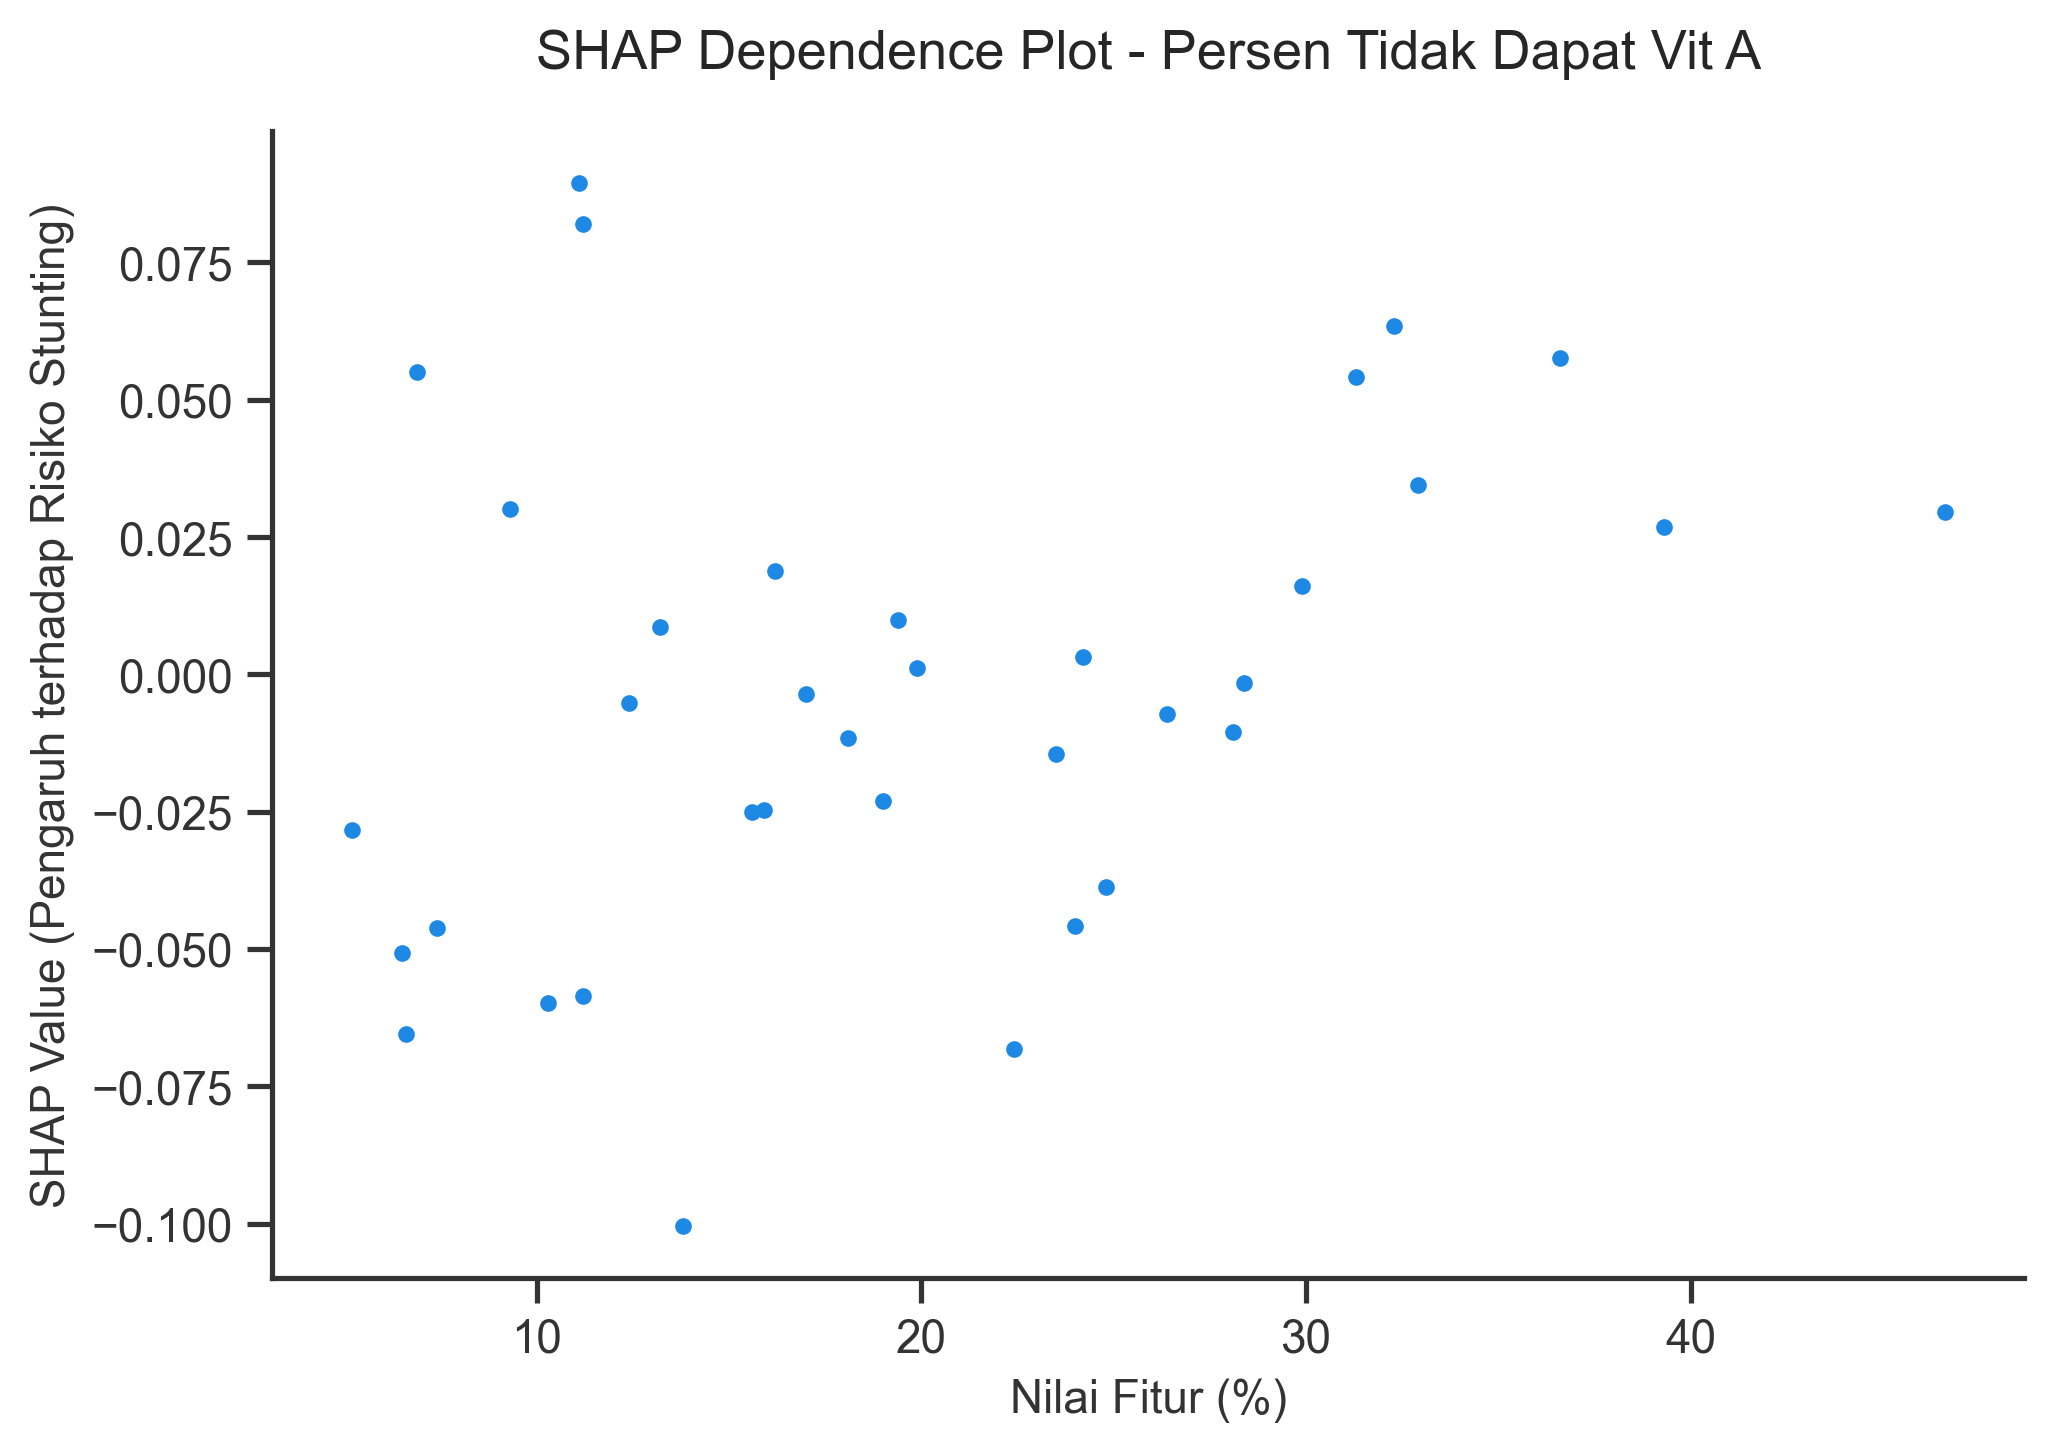
\includegraphics[width=0.48\textwidth]{figure/hasil_dependence_plot/dependence_persen_tidak_dapat_vit_a.png} \hfill
    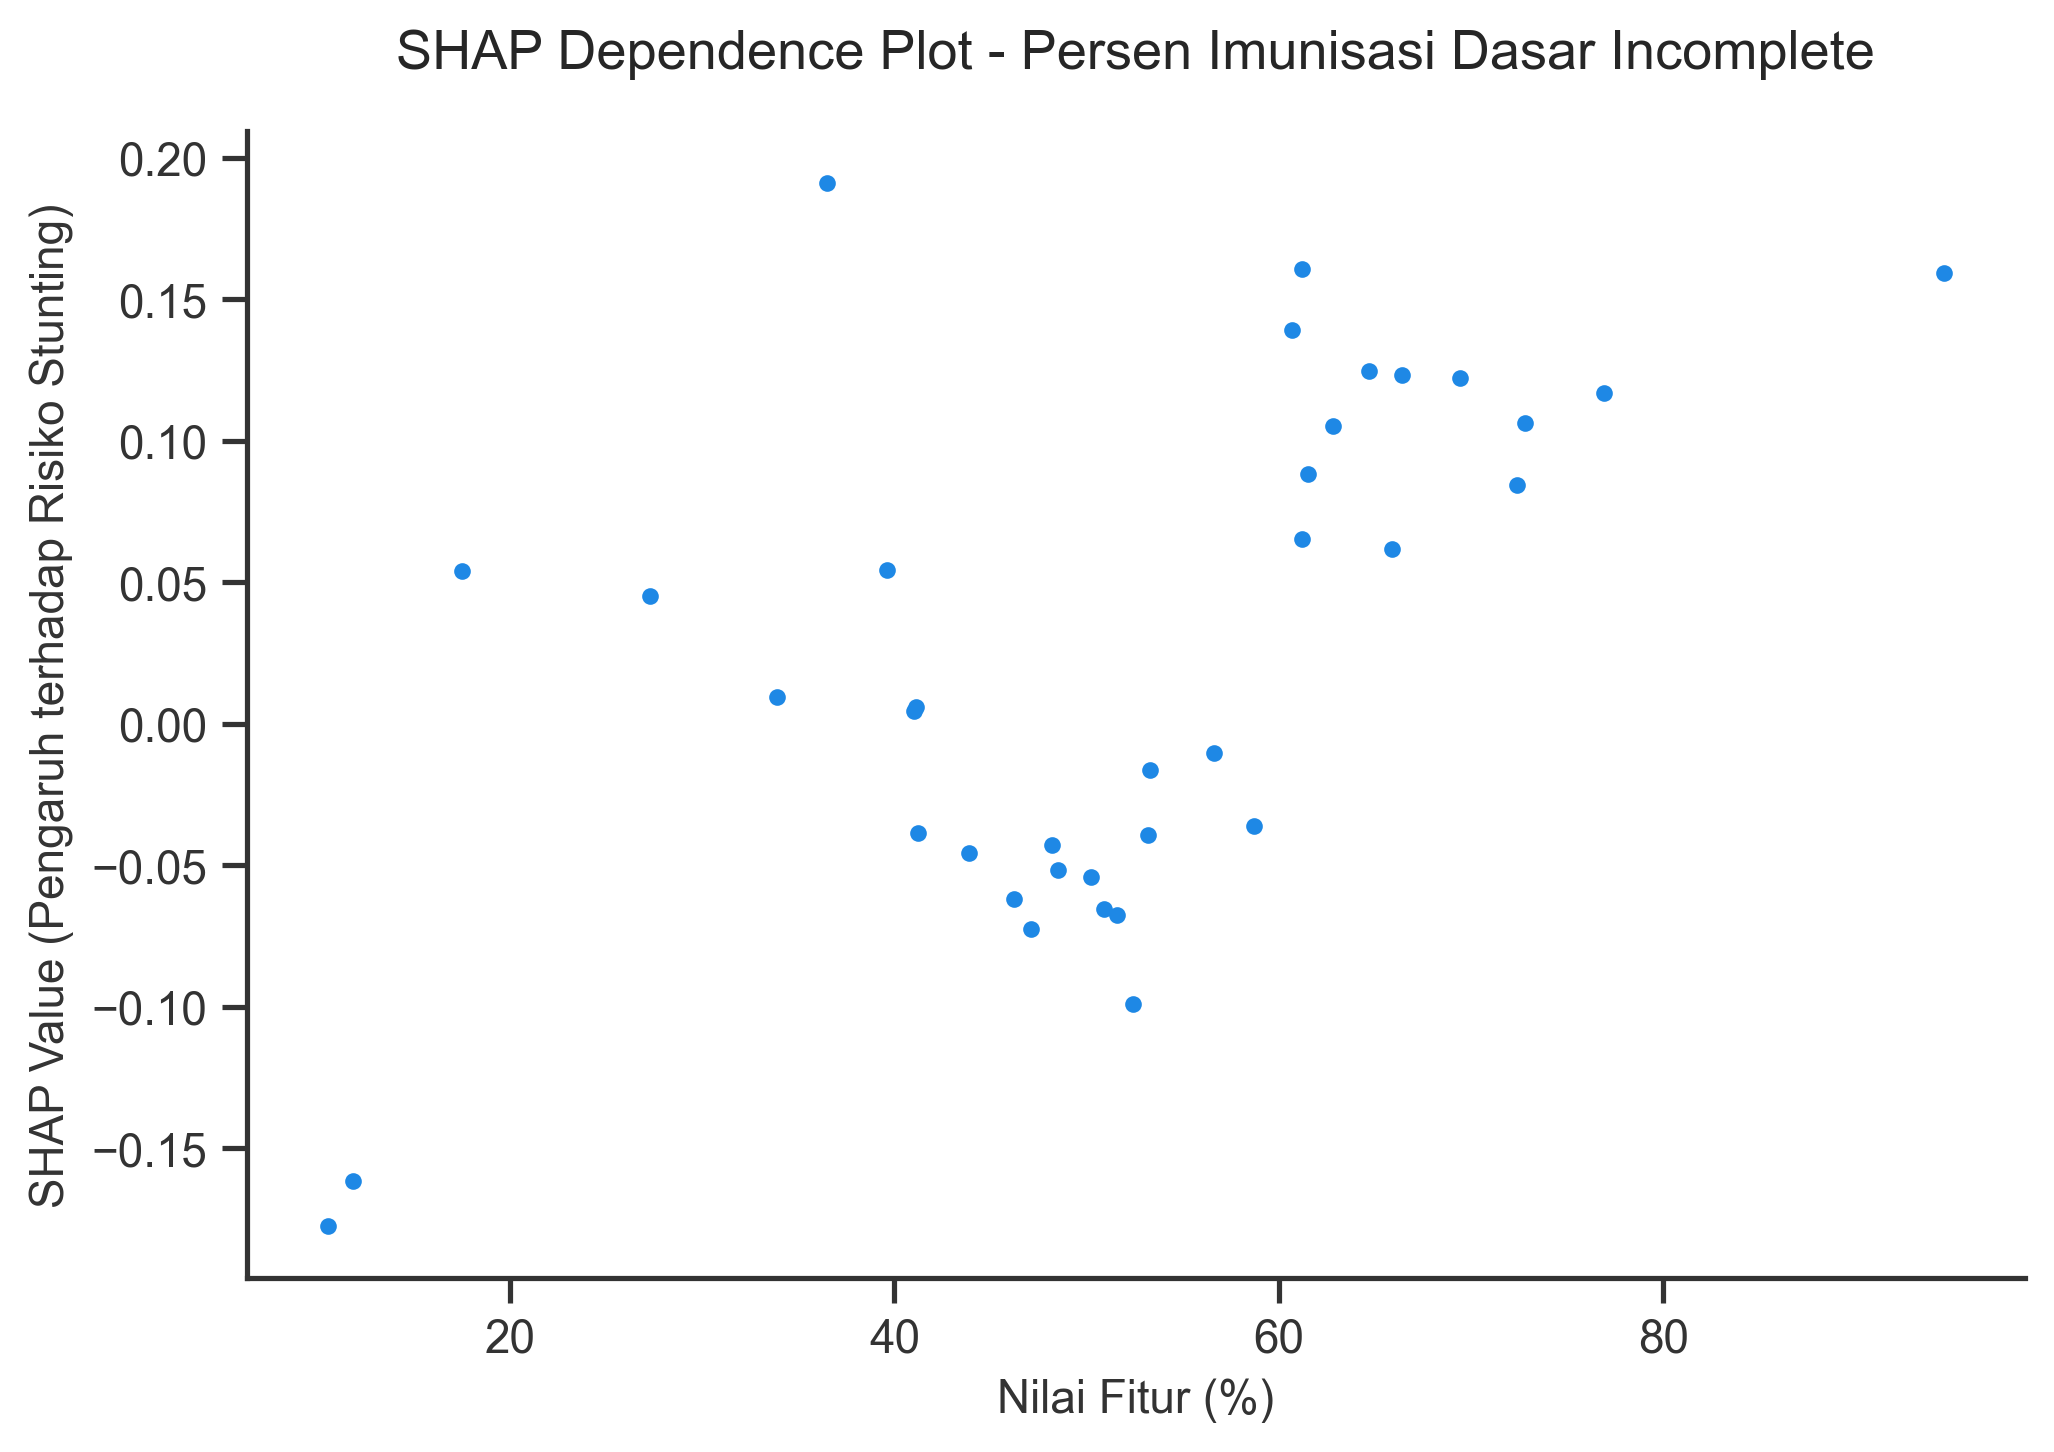
\includegraphics[width=0.48\textwidth]{figure/hasil_dependence_plot/dependence_persen_imunisasi_dasar_incomplete.png} \\ \vspace{0.2cm}
    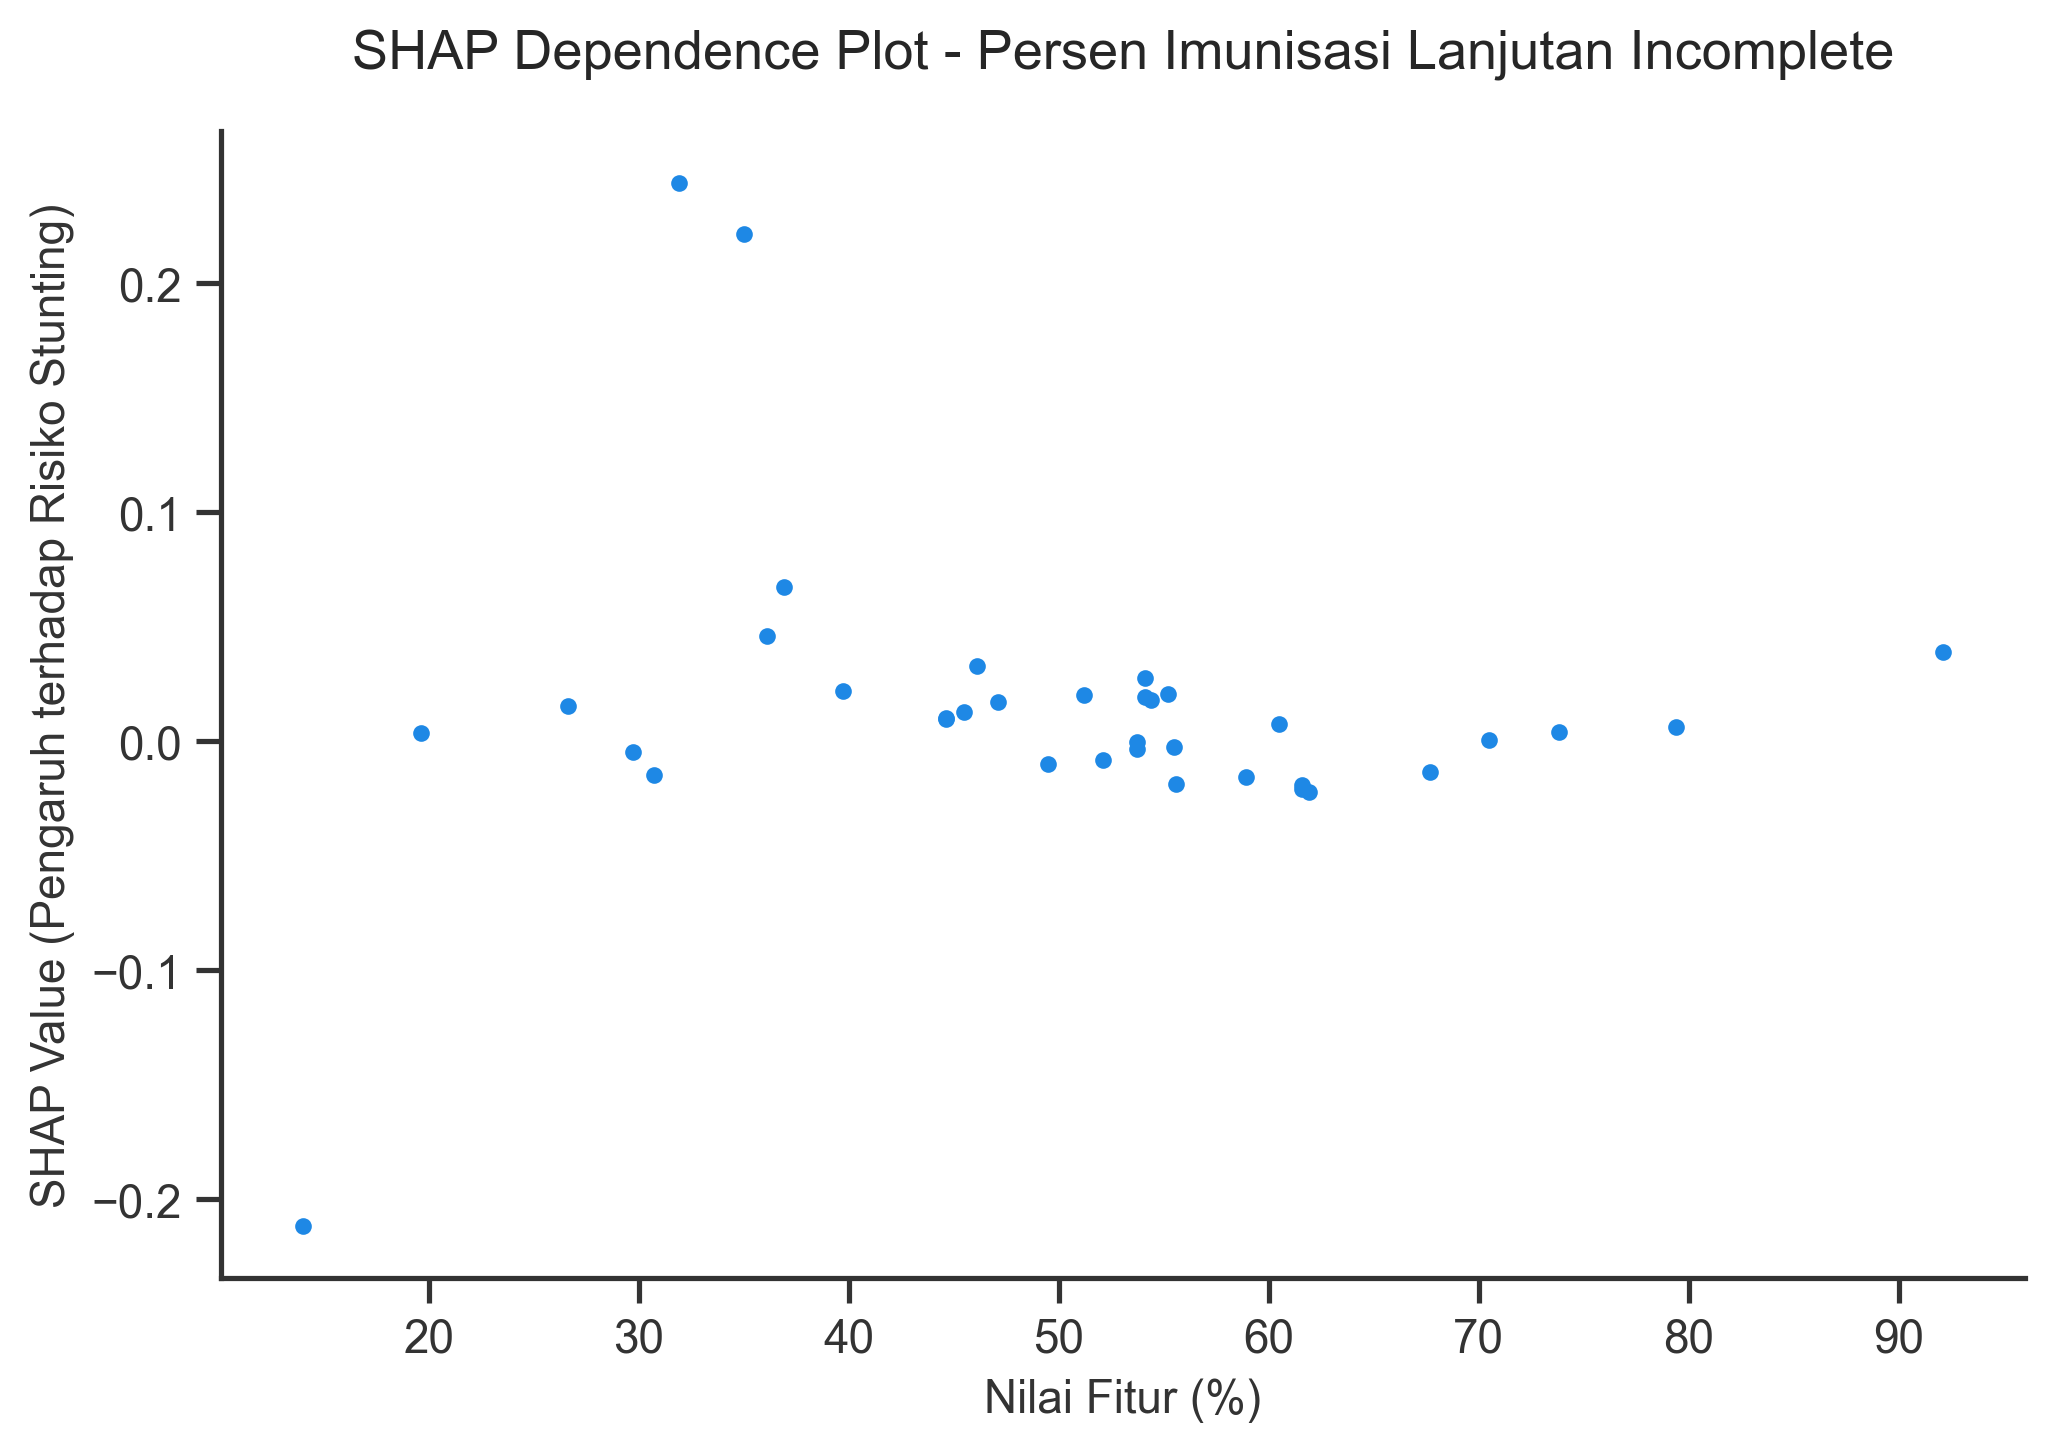
\includegraphics[width=0.48\textwidth]{figure/hasil_dependence_plot/dependence_persen_imunisasi_lanjutan_incomplete.png} \hfill
    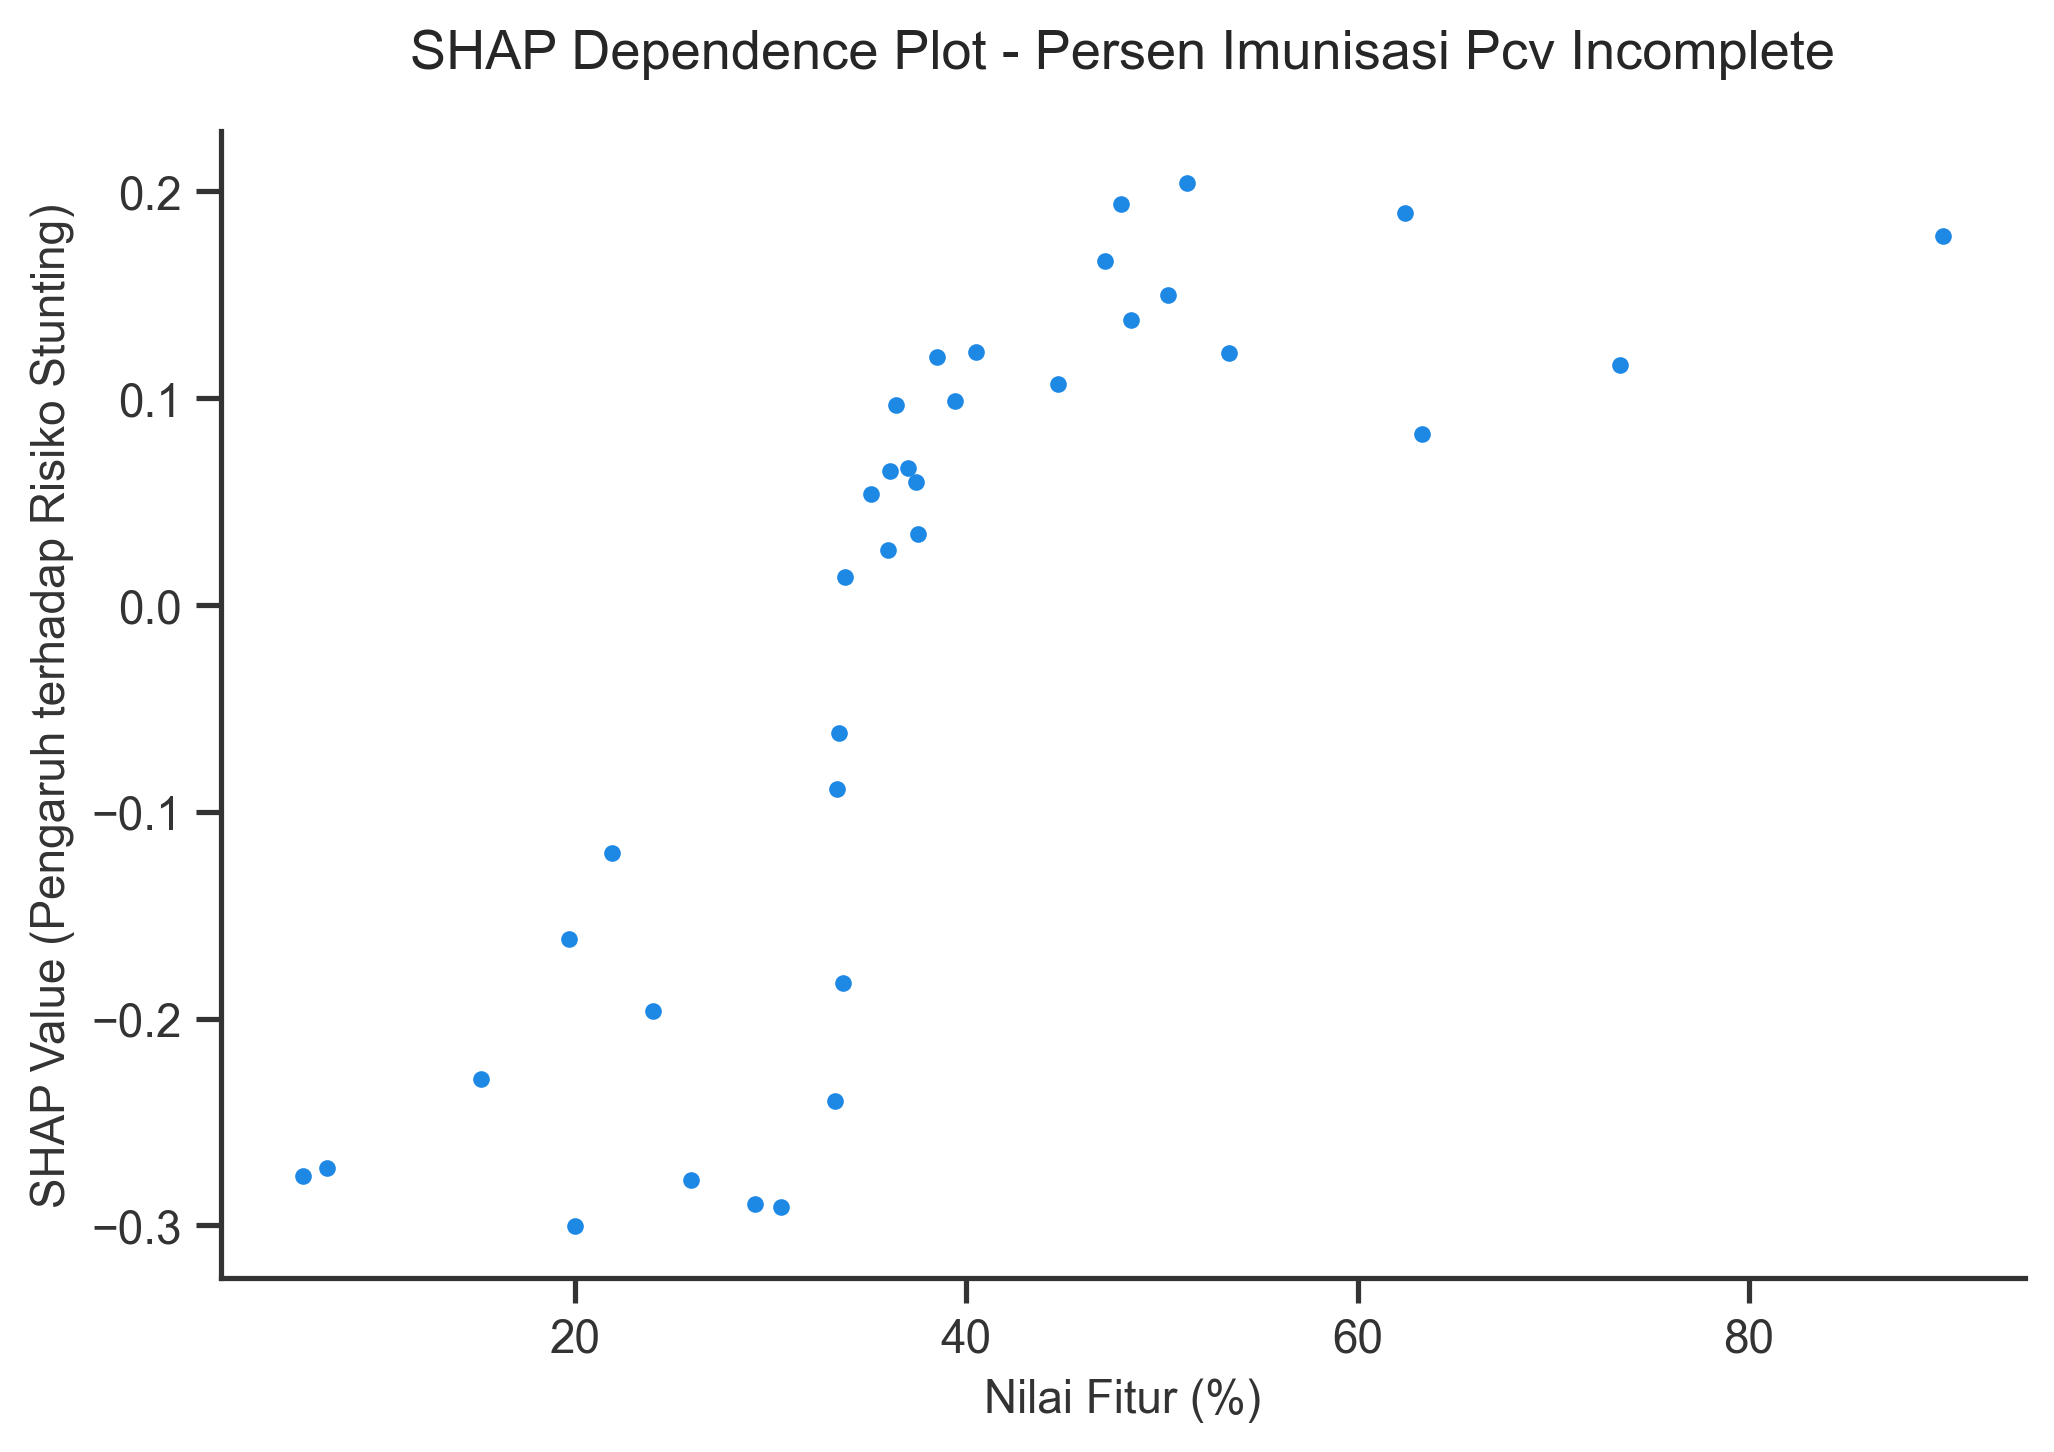
\includegraphics[width=0.48\textwidth]{figure/hasil_dependence_plot/dependence_persen_imunisasi_pcv_incomplete.png} \\ \vspace{0.2cm}
    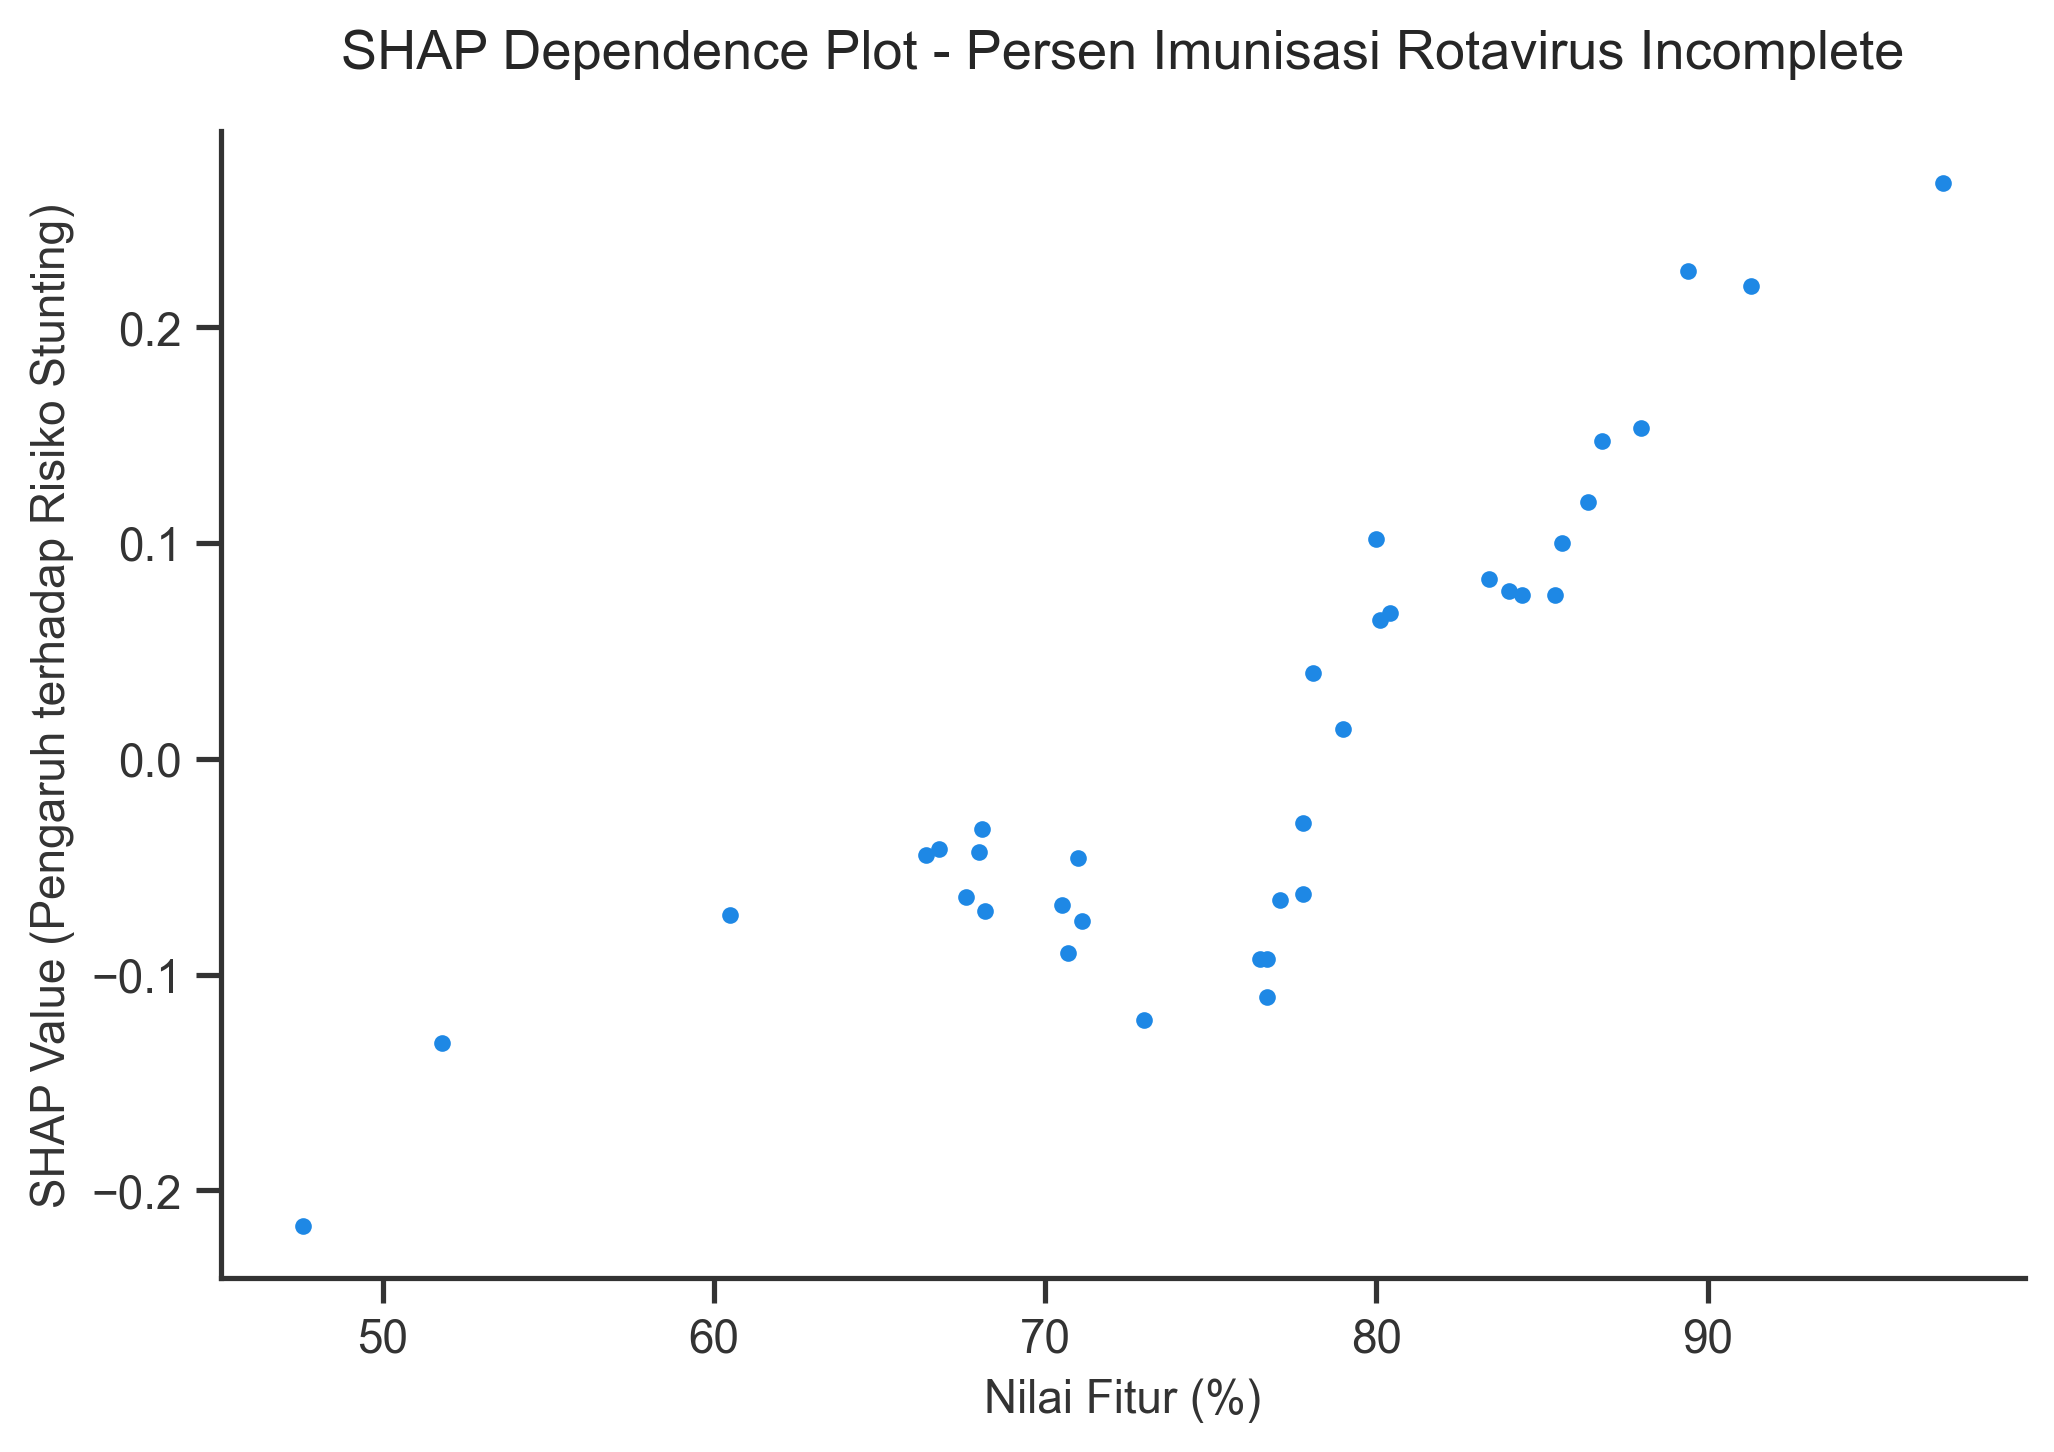
\includegraphics[width=0.48\textwidth]{figure/hasil_dependence_plot/dependence_persen_imunisasi_rotavirus_incomplete.png} \hfill
    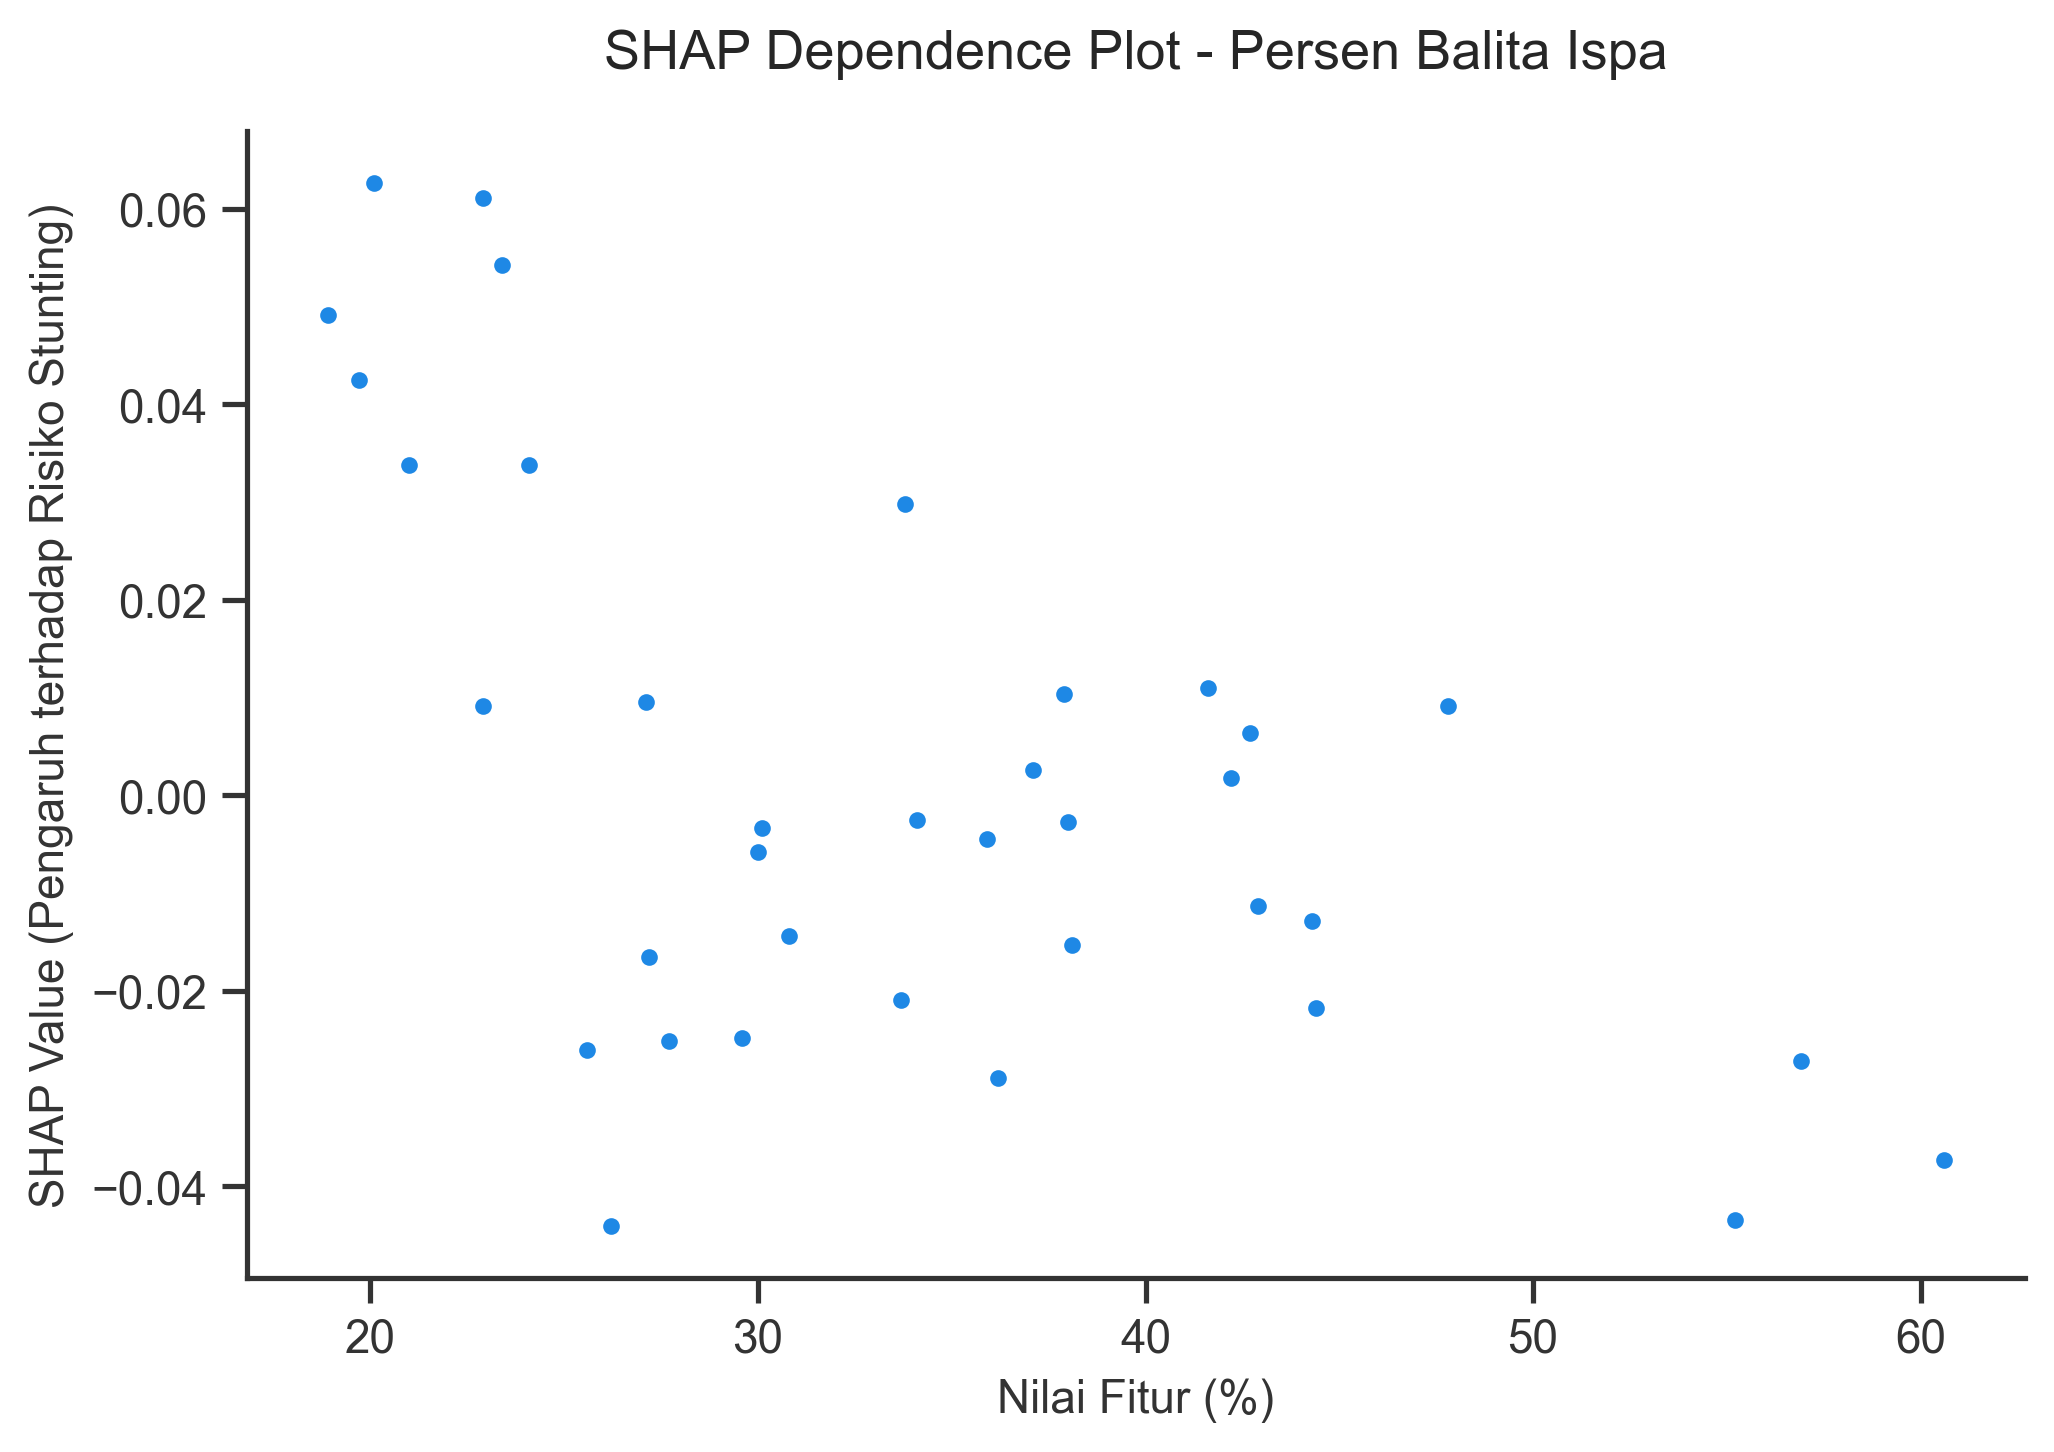
\includegraphics[width=0.48\textwidth]{figure/hasil_dependence_plot/dependence_persen_balita_ispa.png}
\end{figure}

\newpage
\begin{figure}[H]
    \centering
    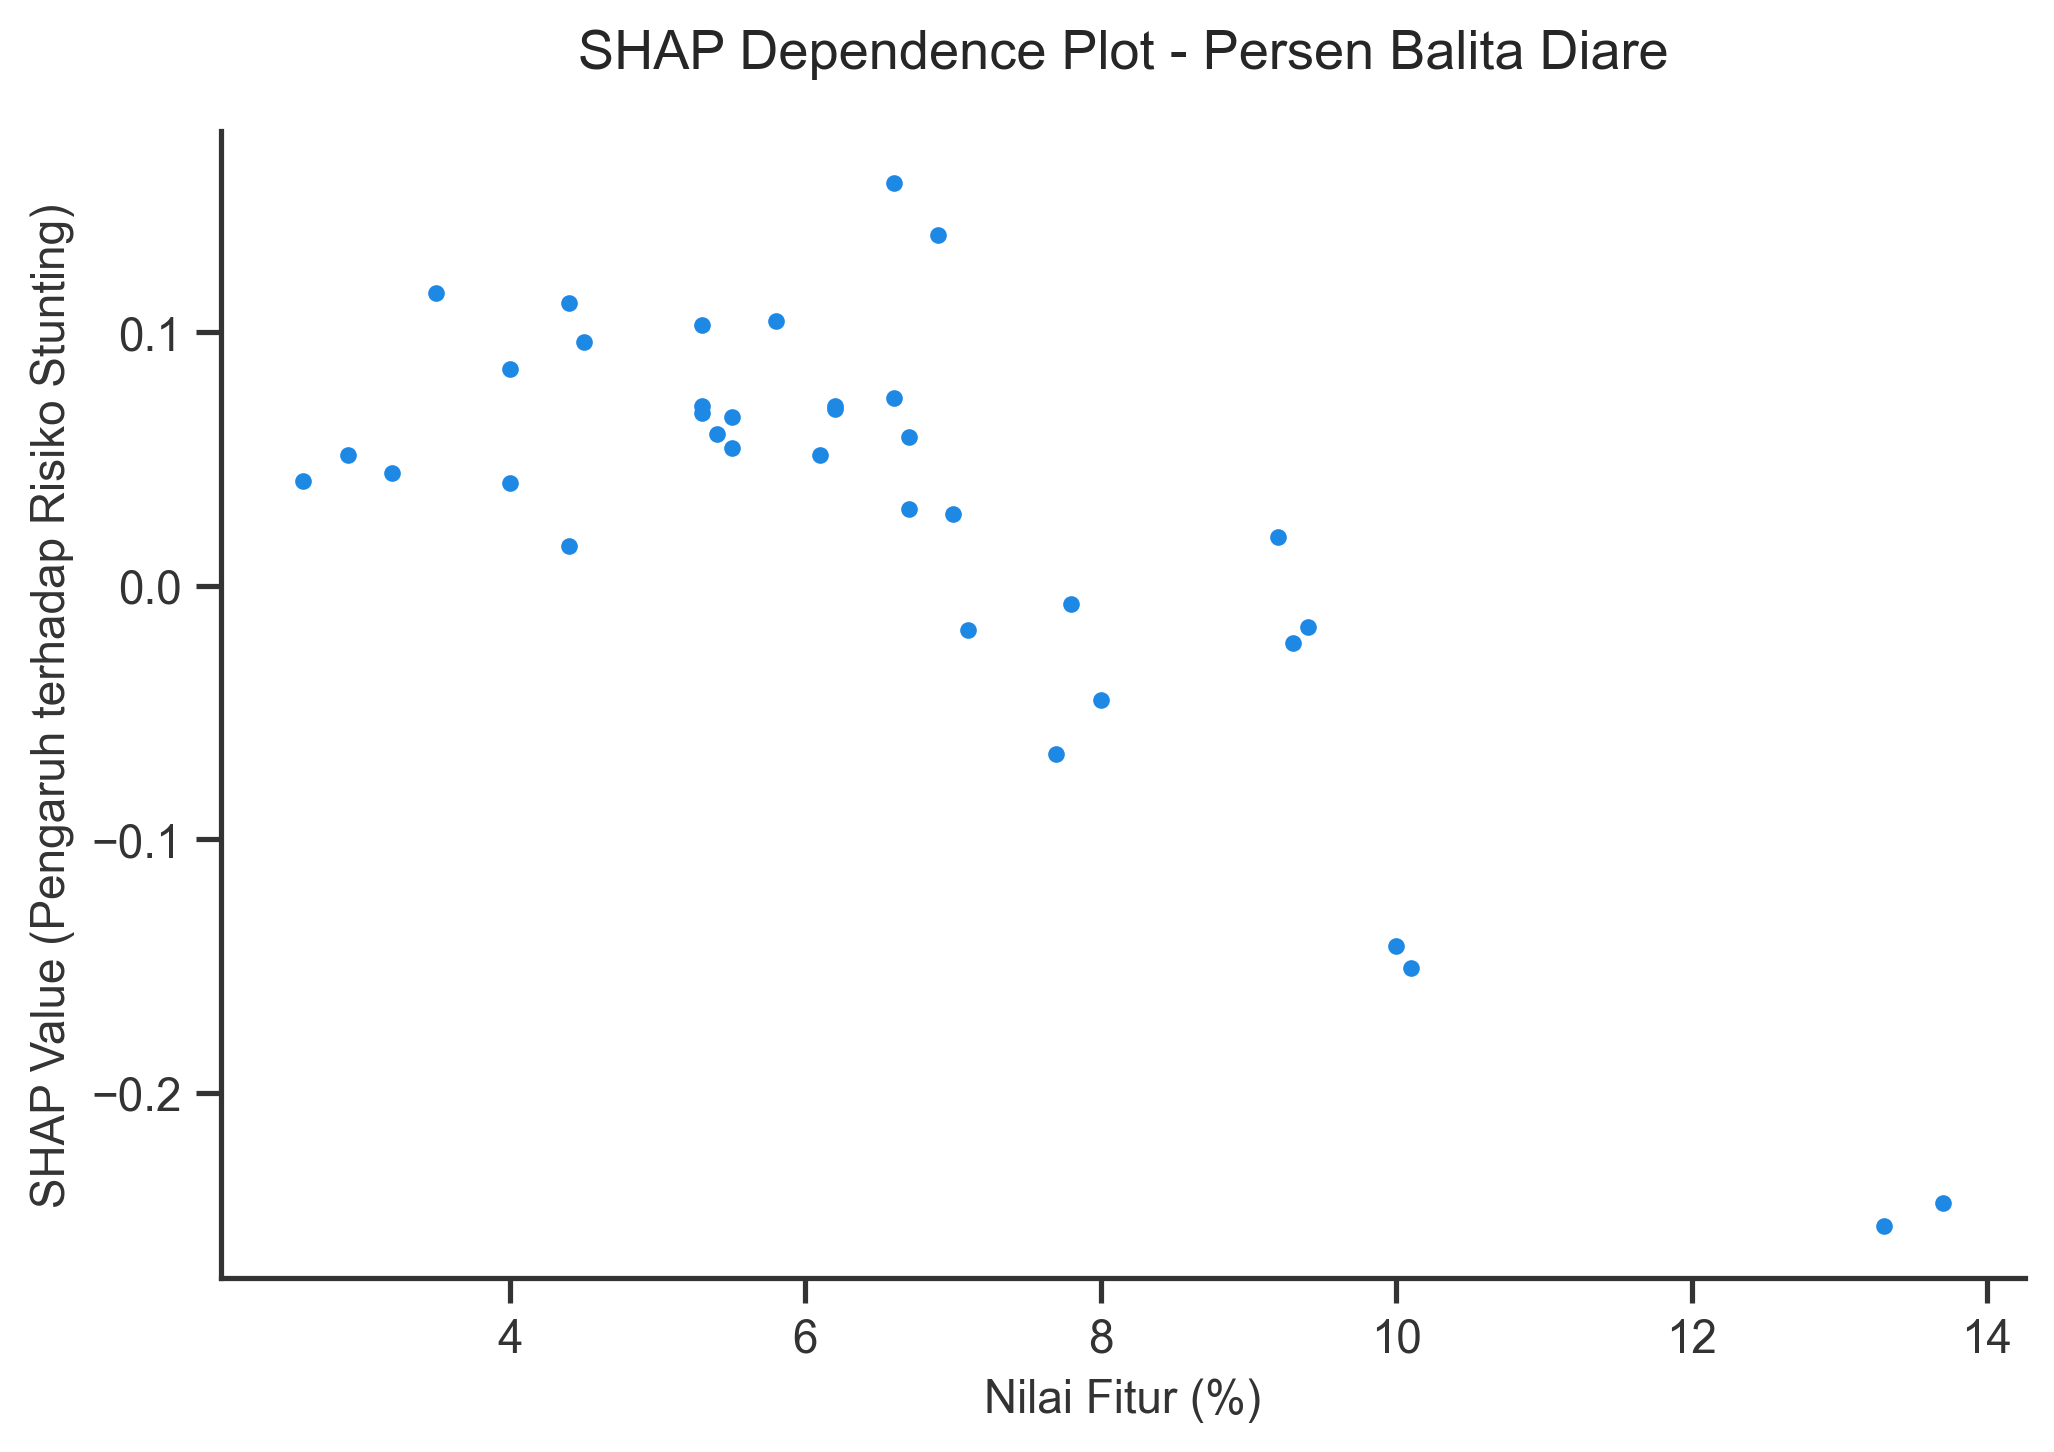
\includegraphics[width=0.48\textwidth]{figure/hasil_dependence_plot/dependence_persen_balita_diare.png} \hfill
    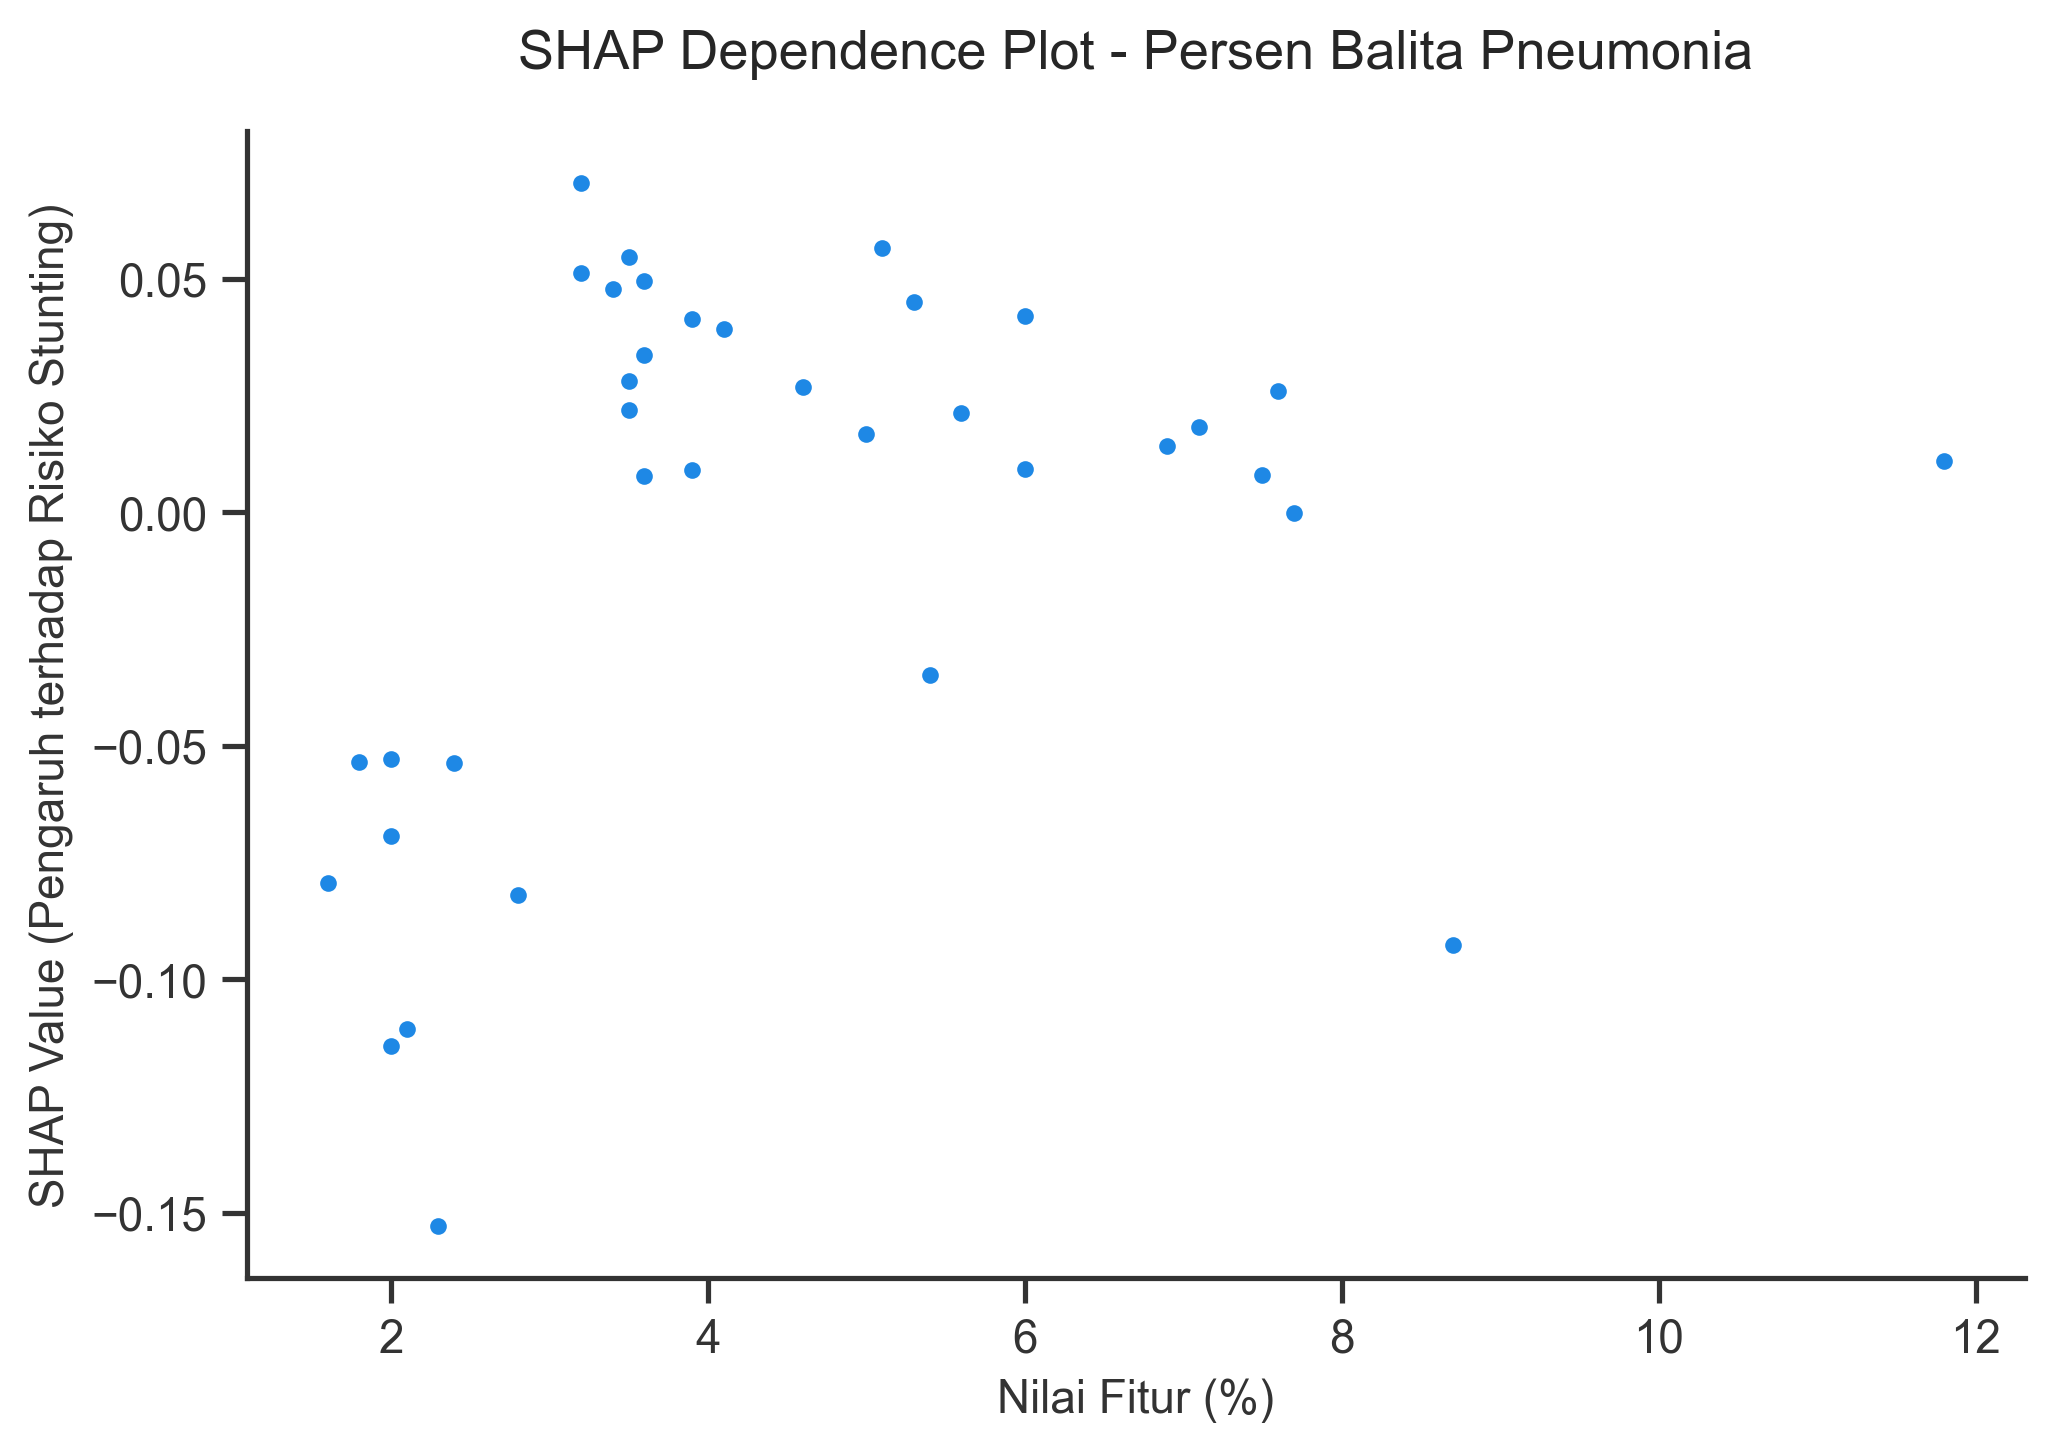
\includegraphics[width=0.48\textwidth]{figure/hasil_dependence_plot/dependence_persen_balita_pneumonia.png} \\ \vspace{0.2cm}
    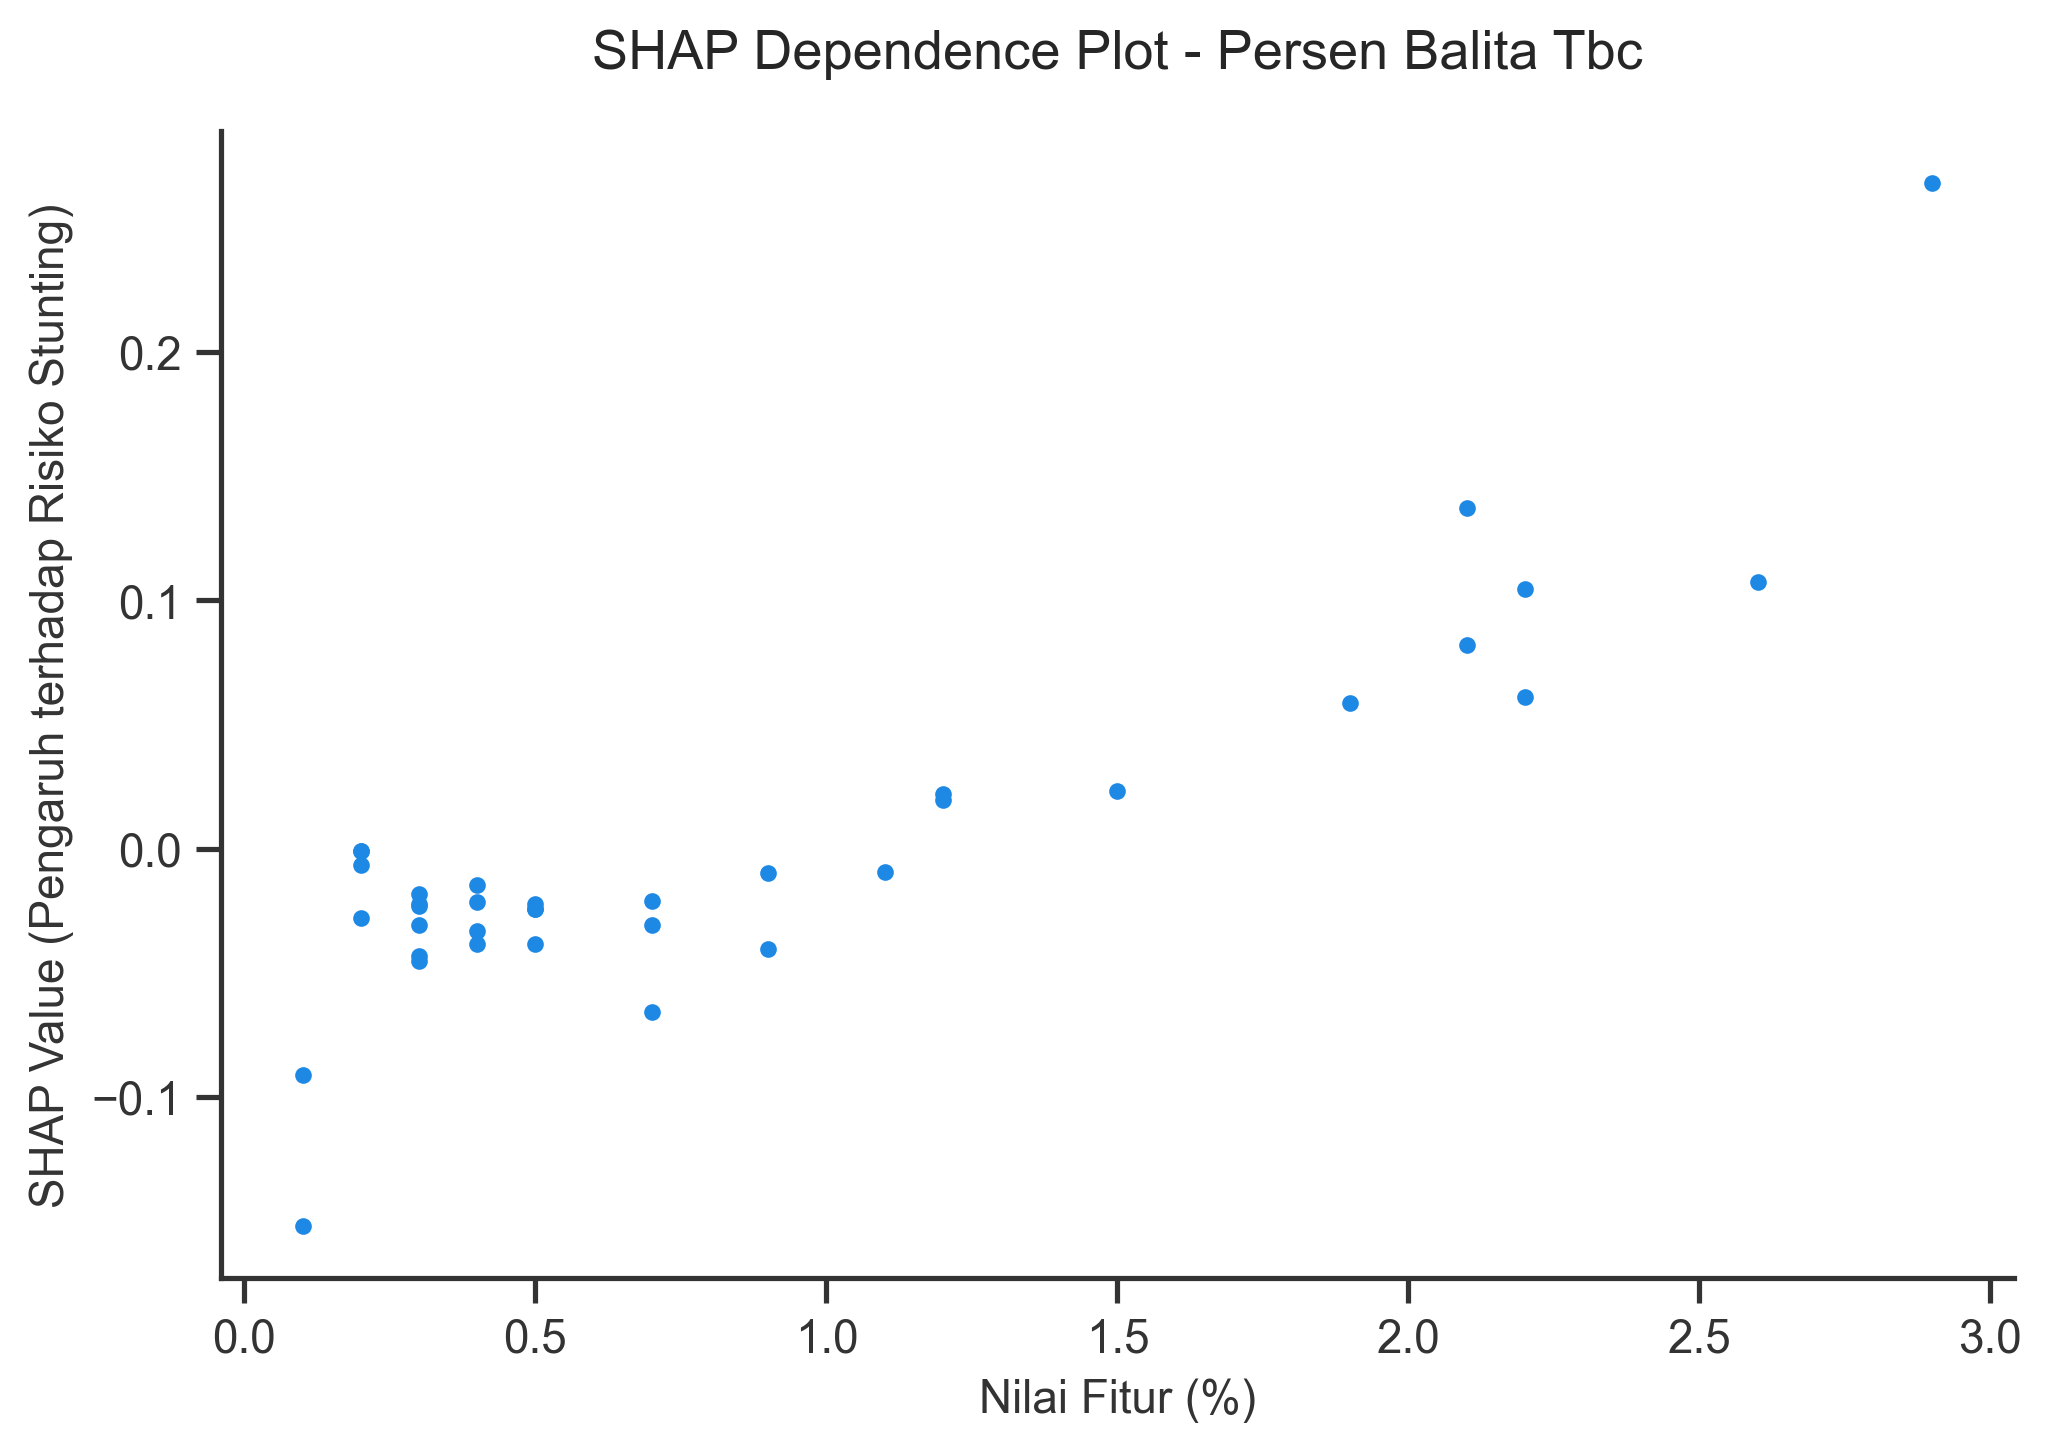
\includegraphics[width=0.48\textwidth]{figure/hasil_dependence_plot/dependence_persen_balita_tbc.png} \hfill
    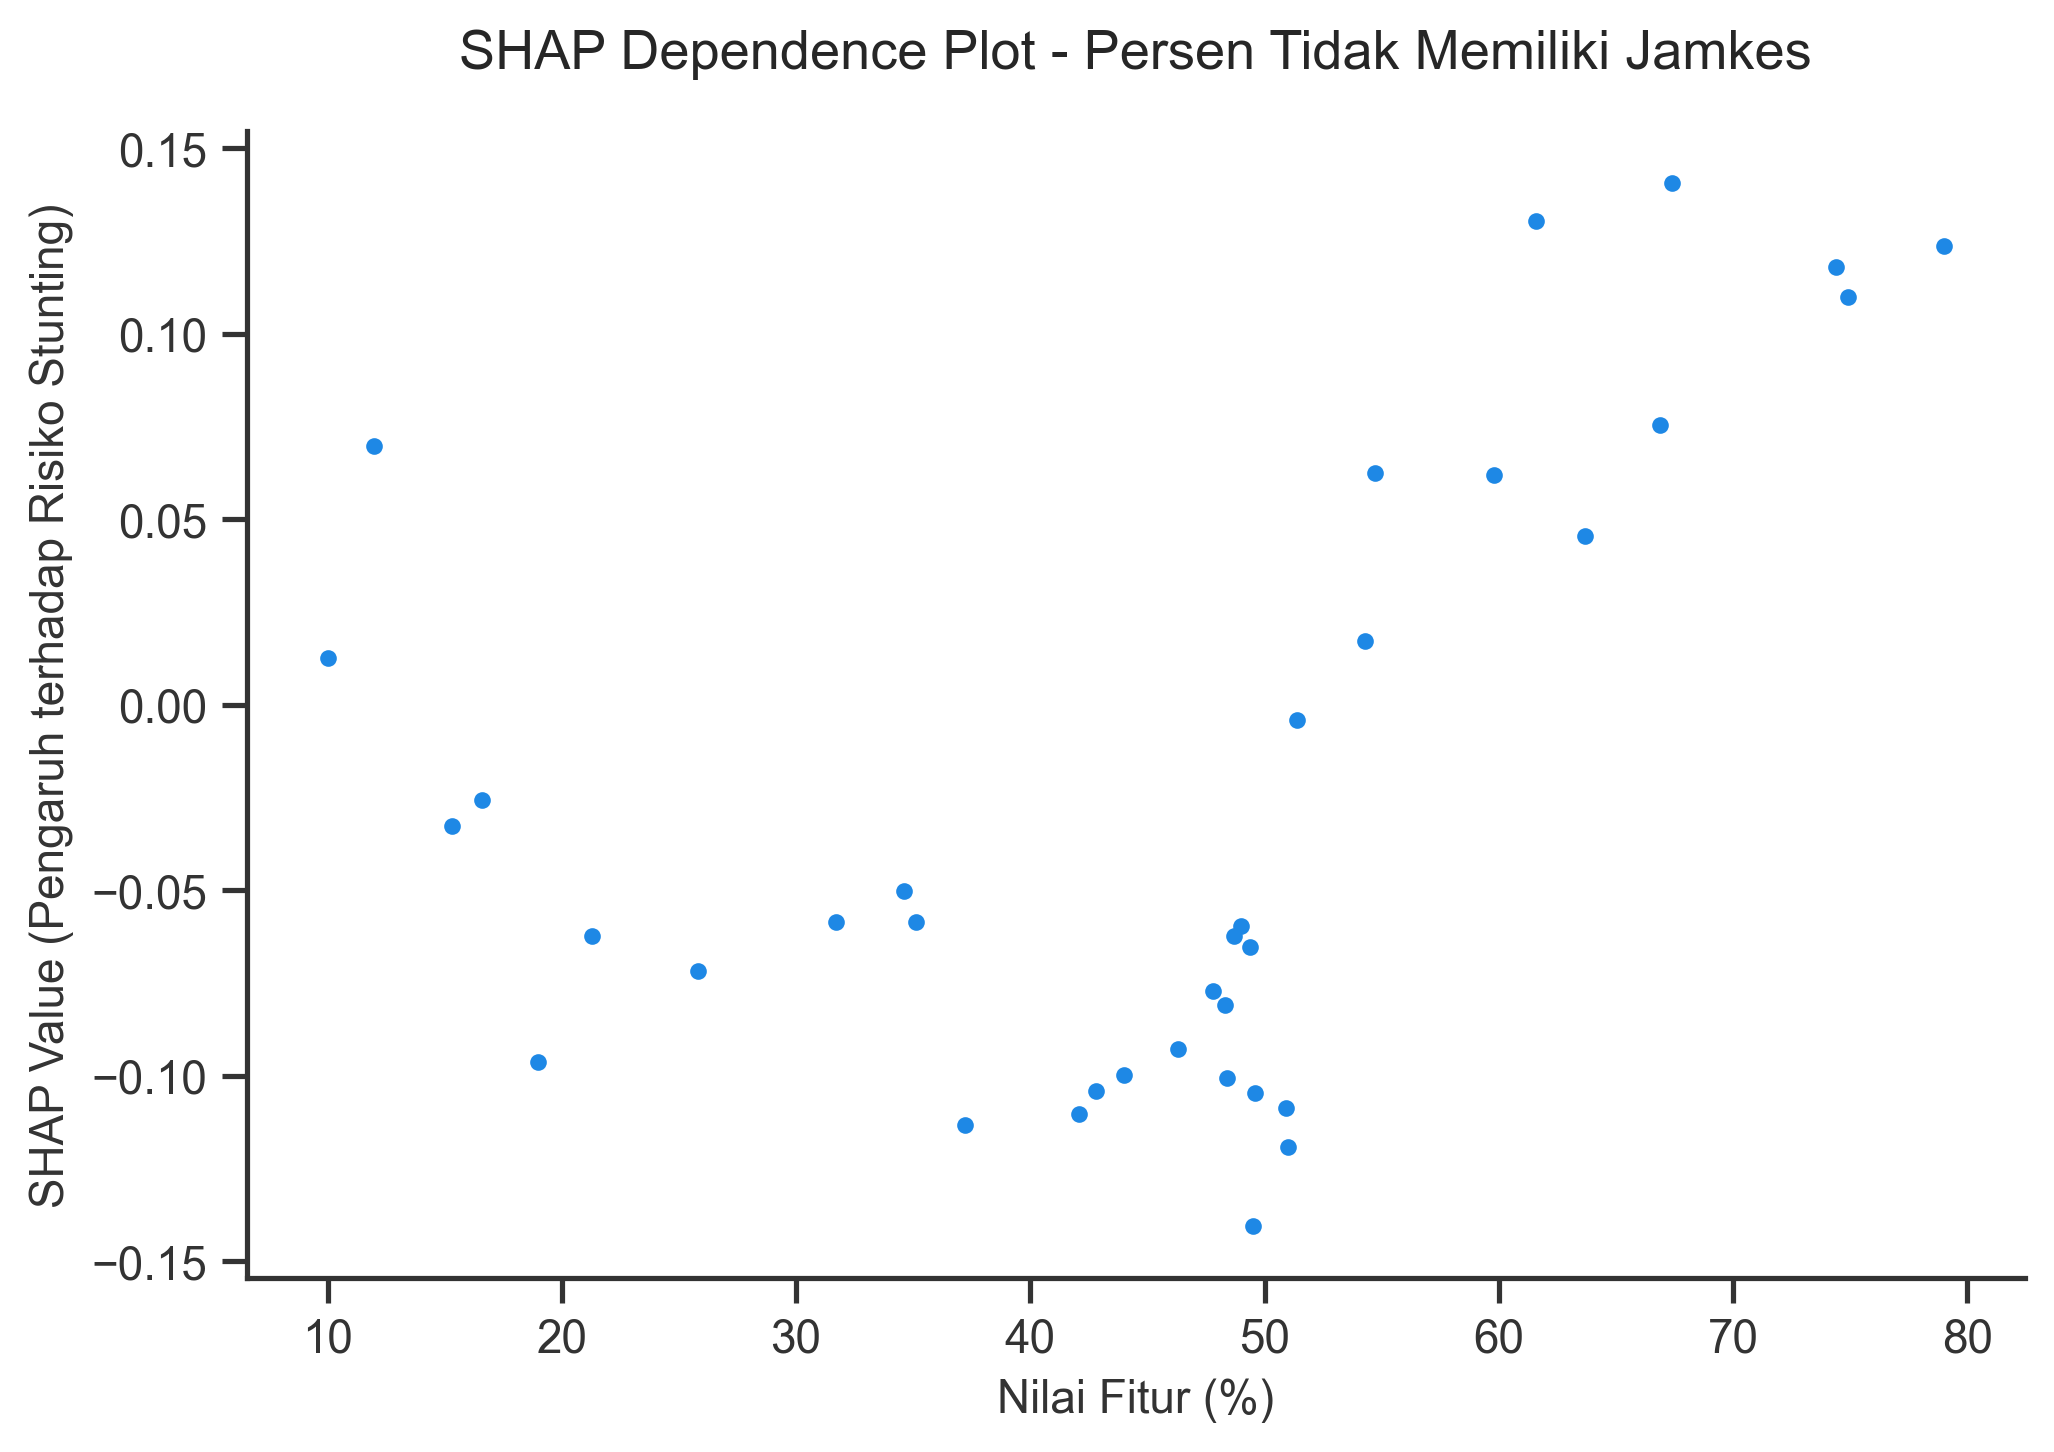
\includegraphics[width=0.48\textwidth]{figure/hasil_dependence_plot/dependence_persen_tidak_memiliki_jamkes.png} \\ \vspace{0.2cm}
    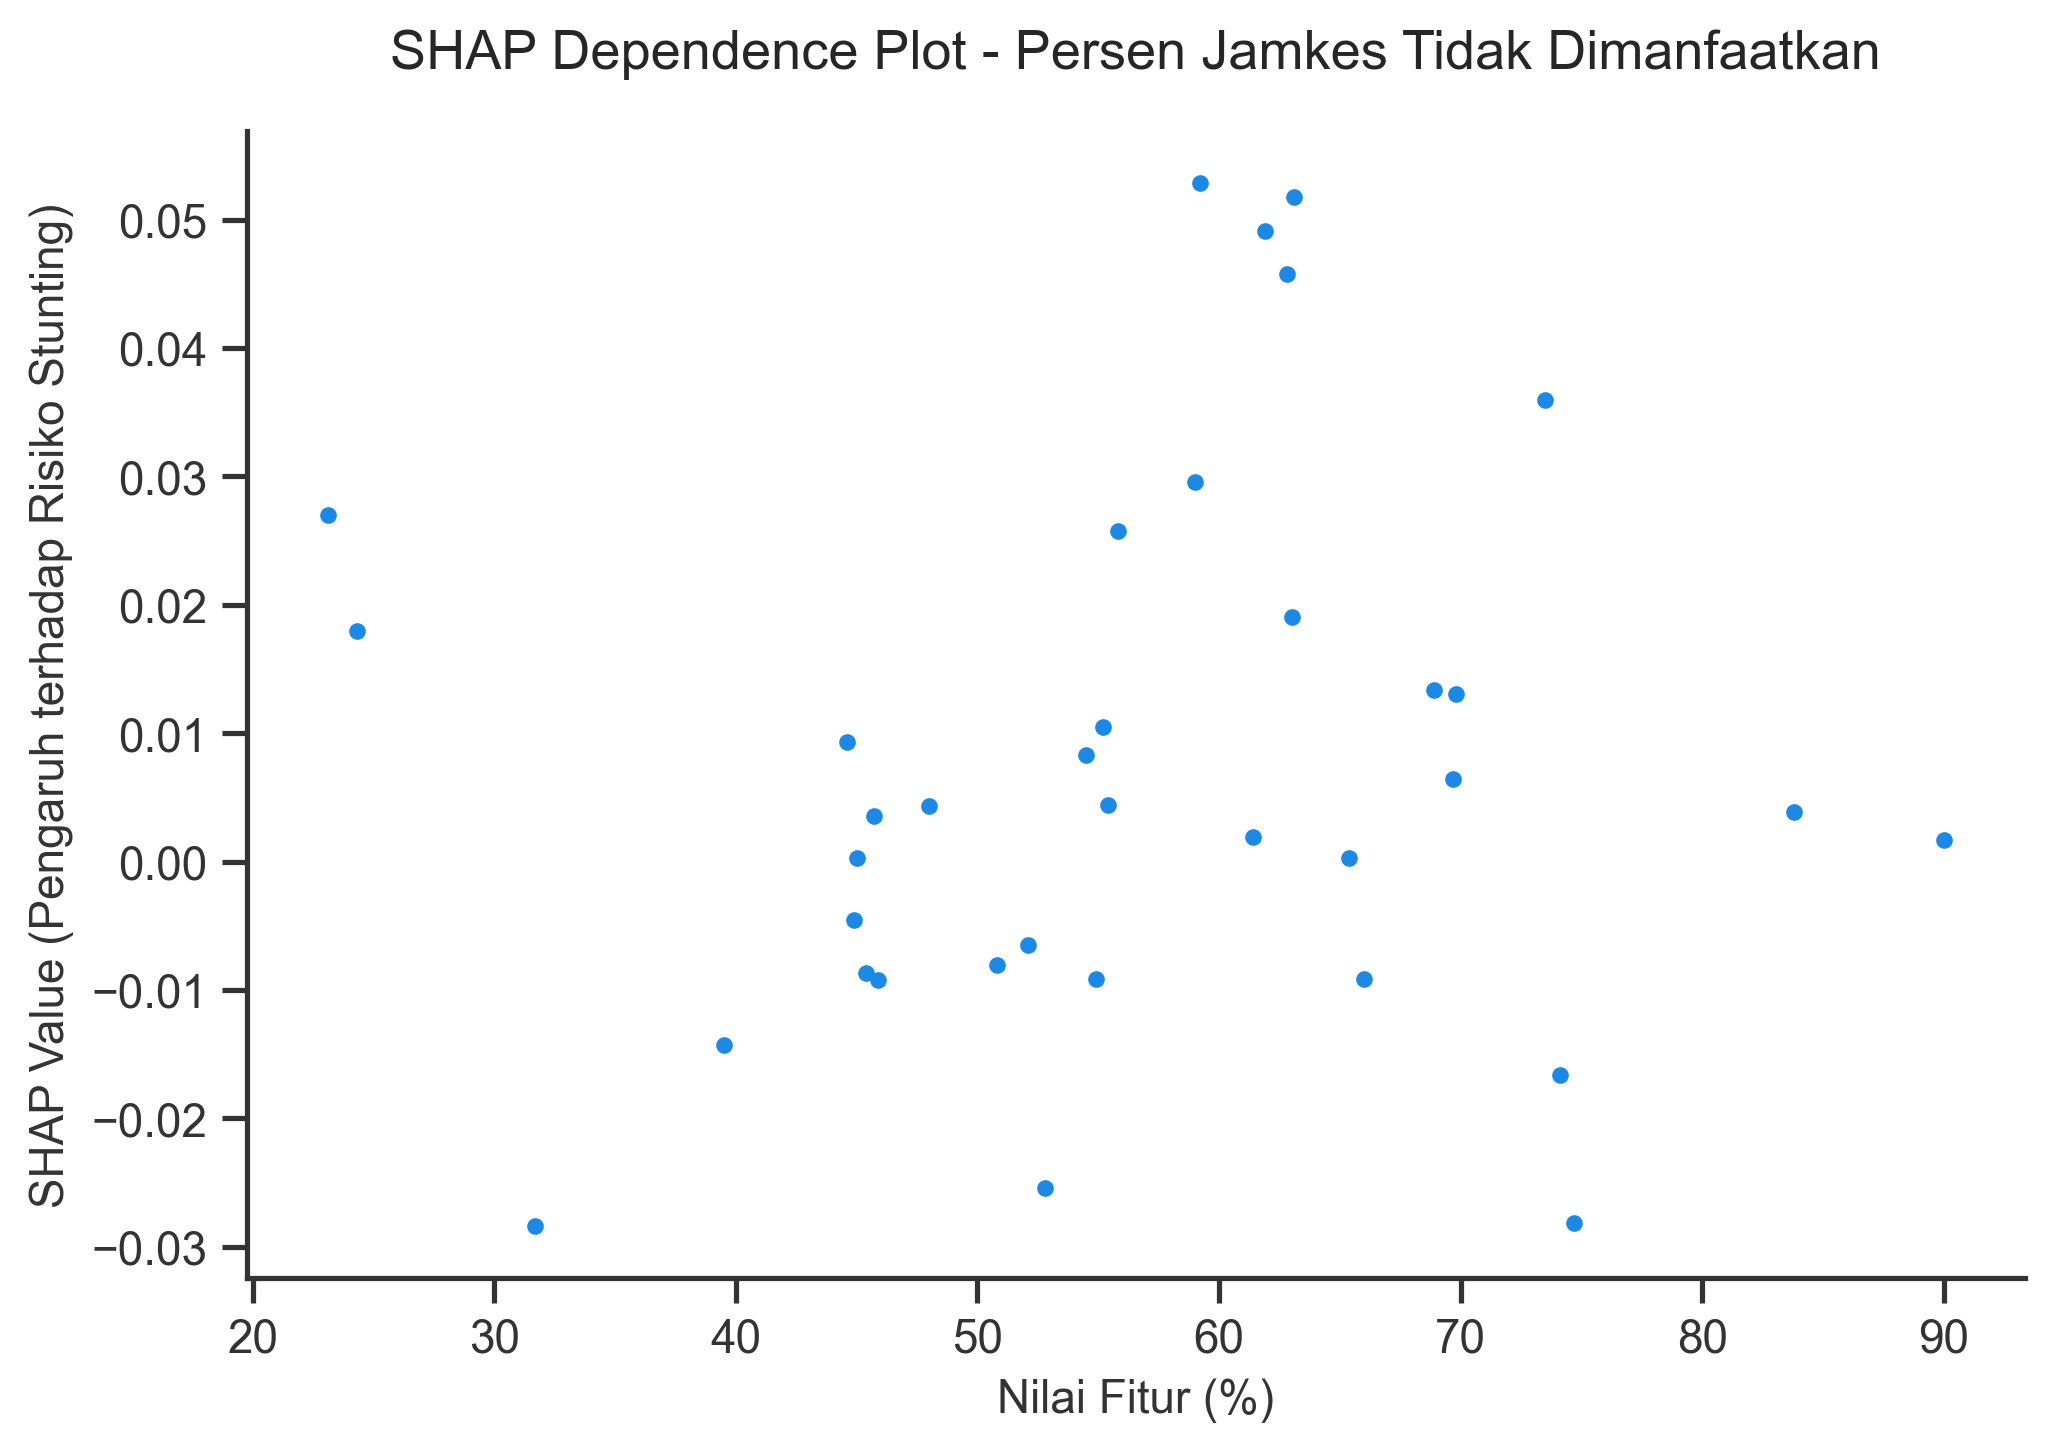
\includegraphics[width=0.48\textwidth]{figure/hasil_dependence_plot/dependence_persen_jamkes_tidak_dimanfaatkan.png} \hfill
    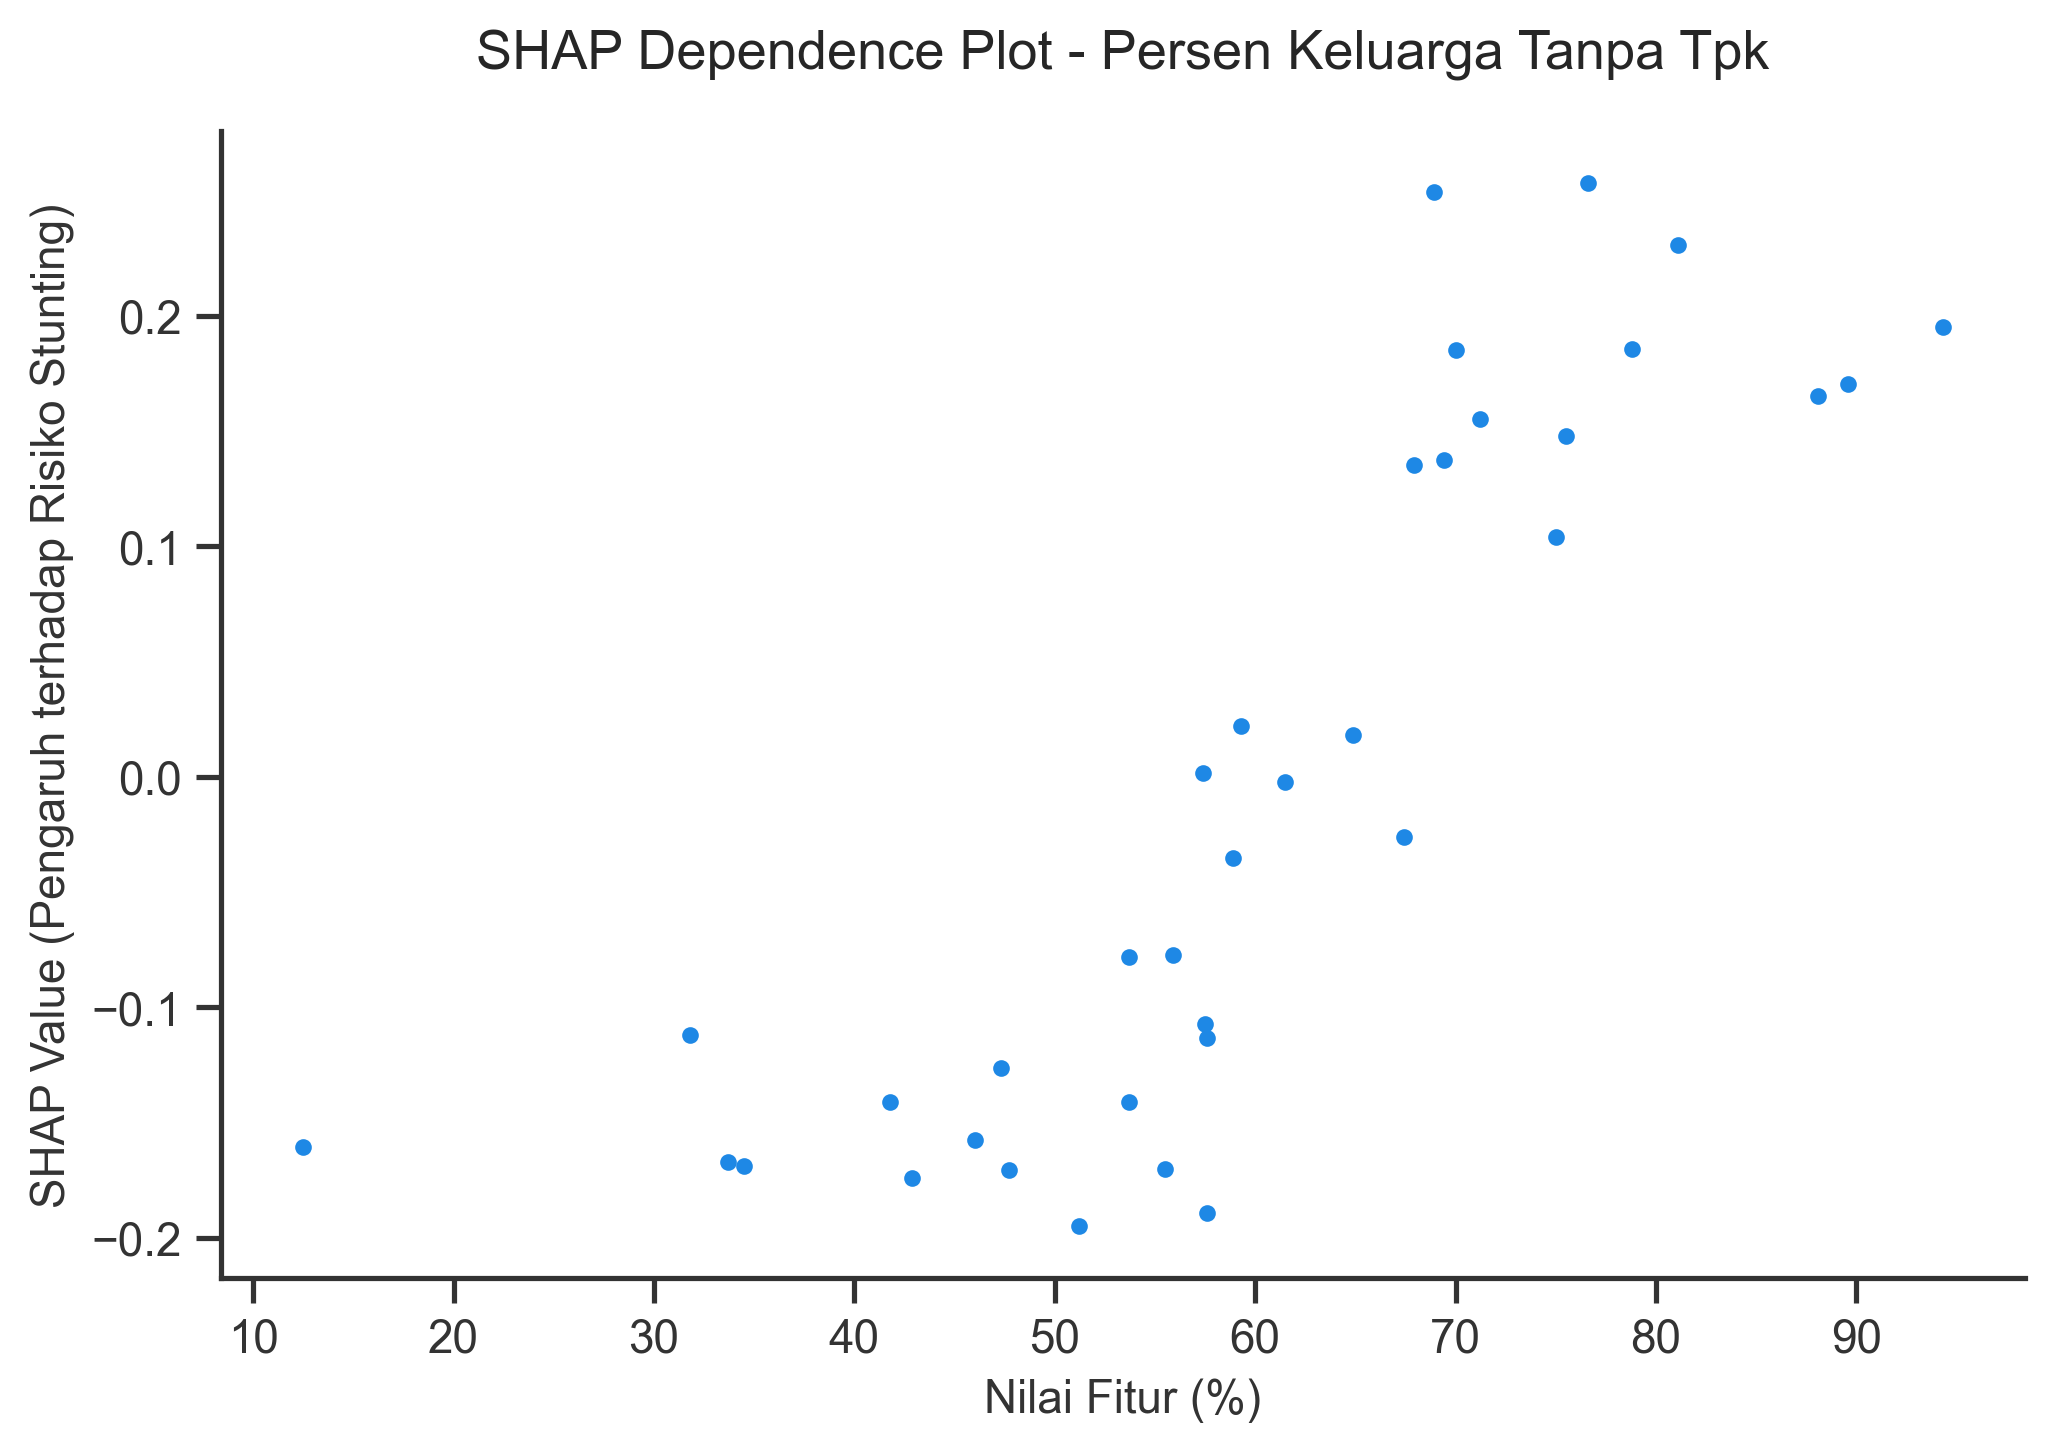
\includegraphics[width=0.48\textwidth]{figure/hasil_dependence_plot/dependence_persen_keluarga_tanpa_tpk.png} \\ \vspace{0.2cm}
    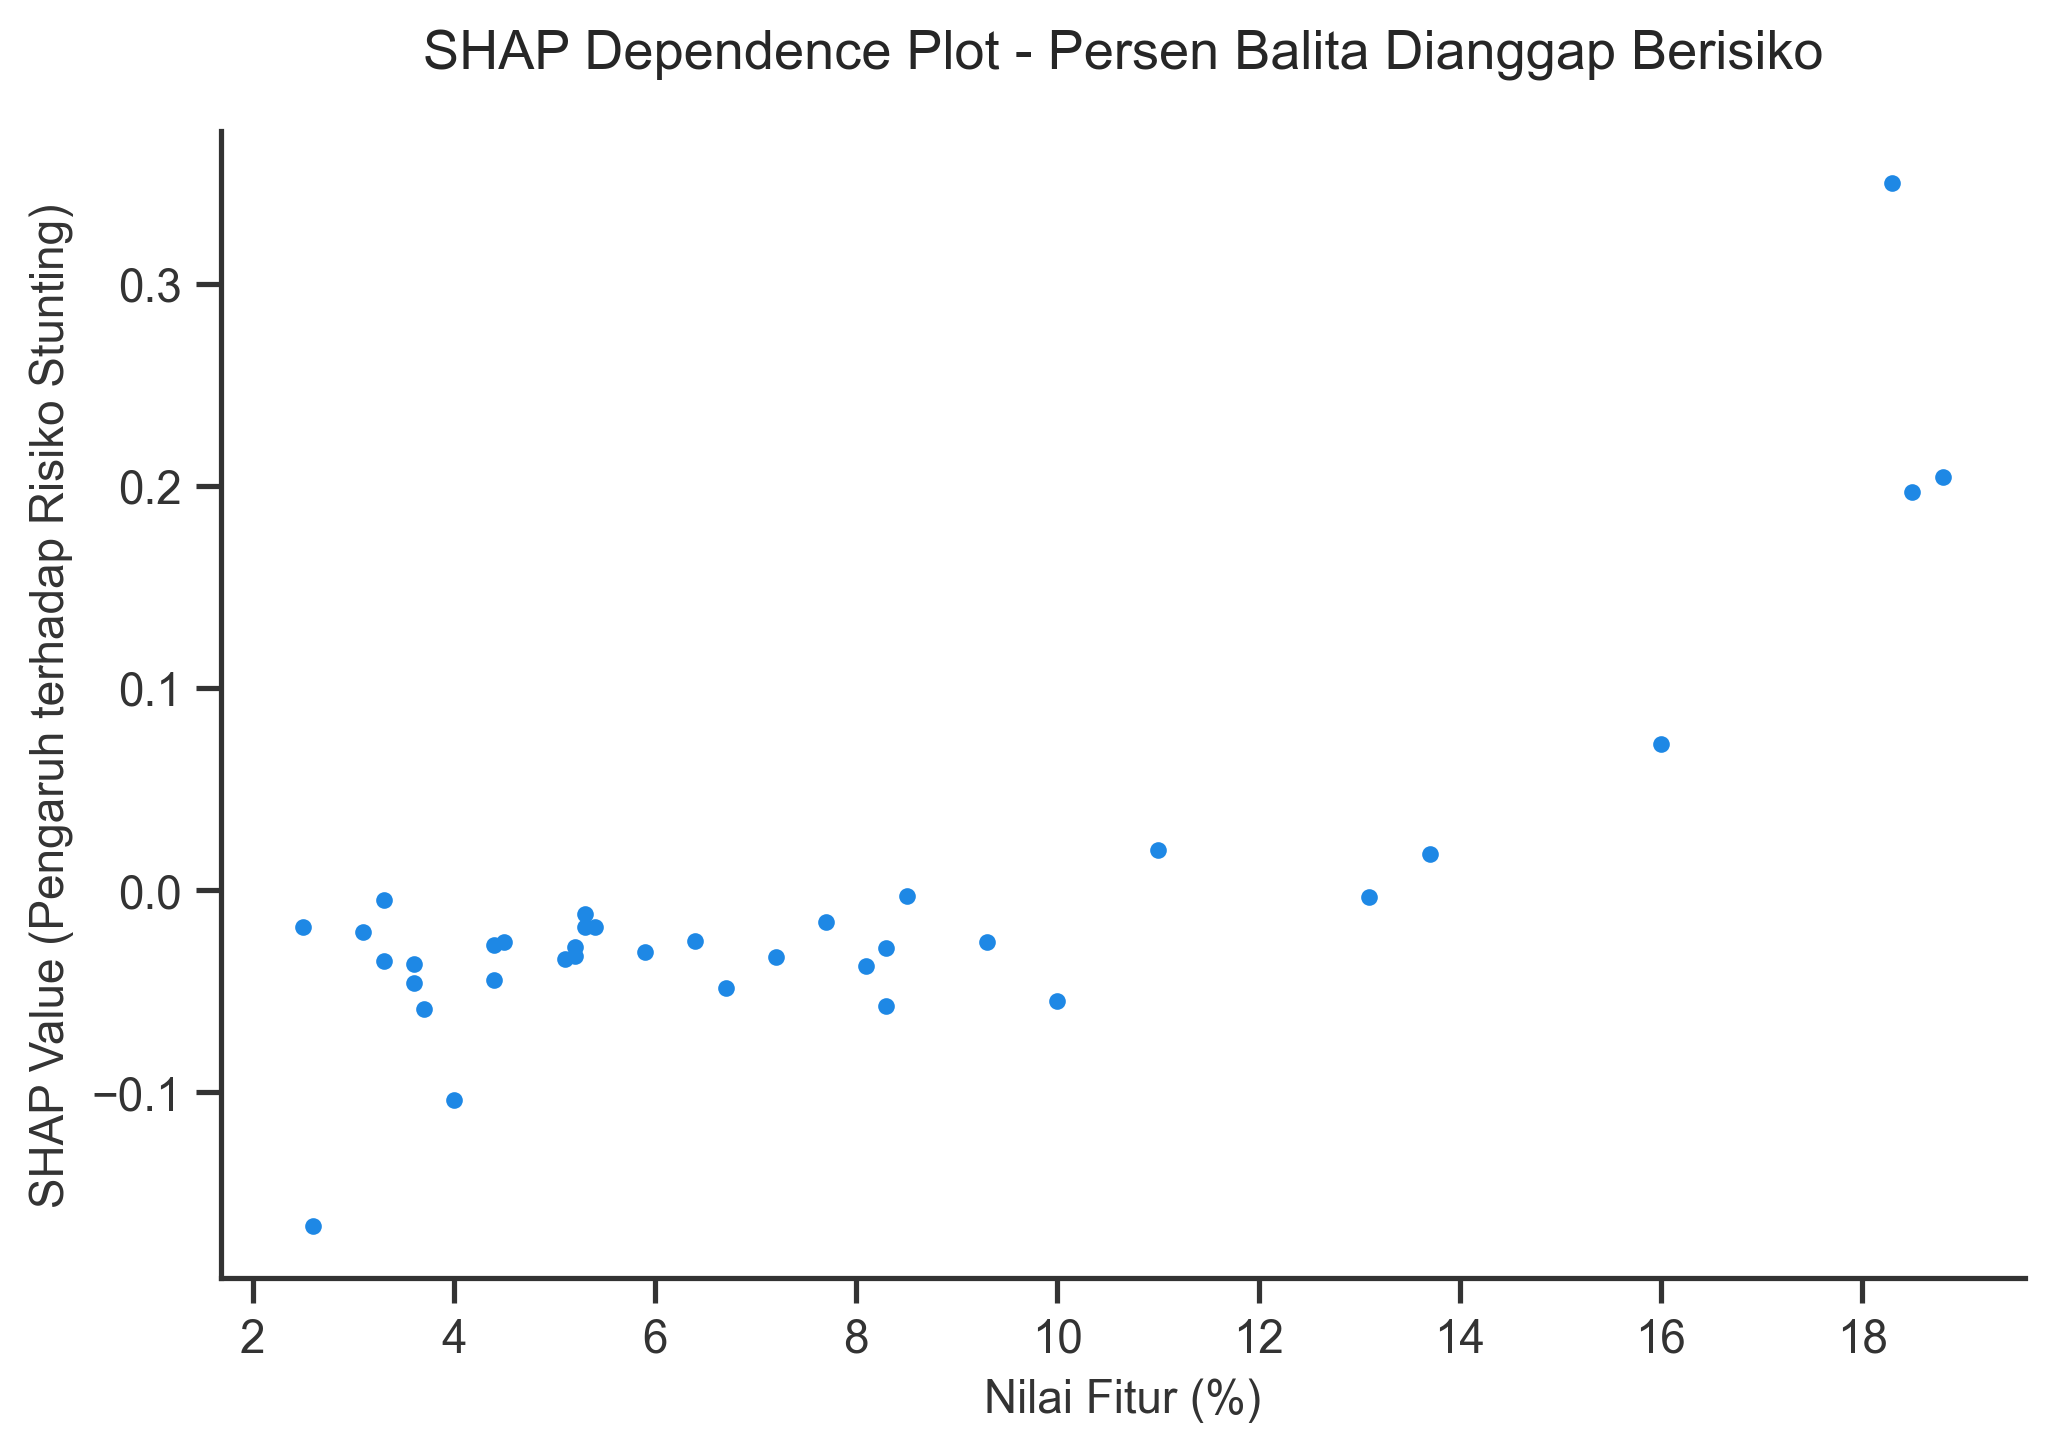
\includegraphics[width=0.48\textwidth]{figure/hasil_dependence_plot/dependence_persen_balita_dianggap_berisiko.png} \hfill
    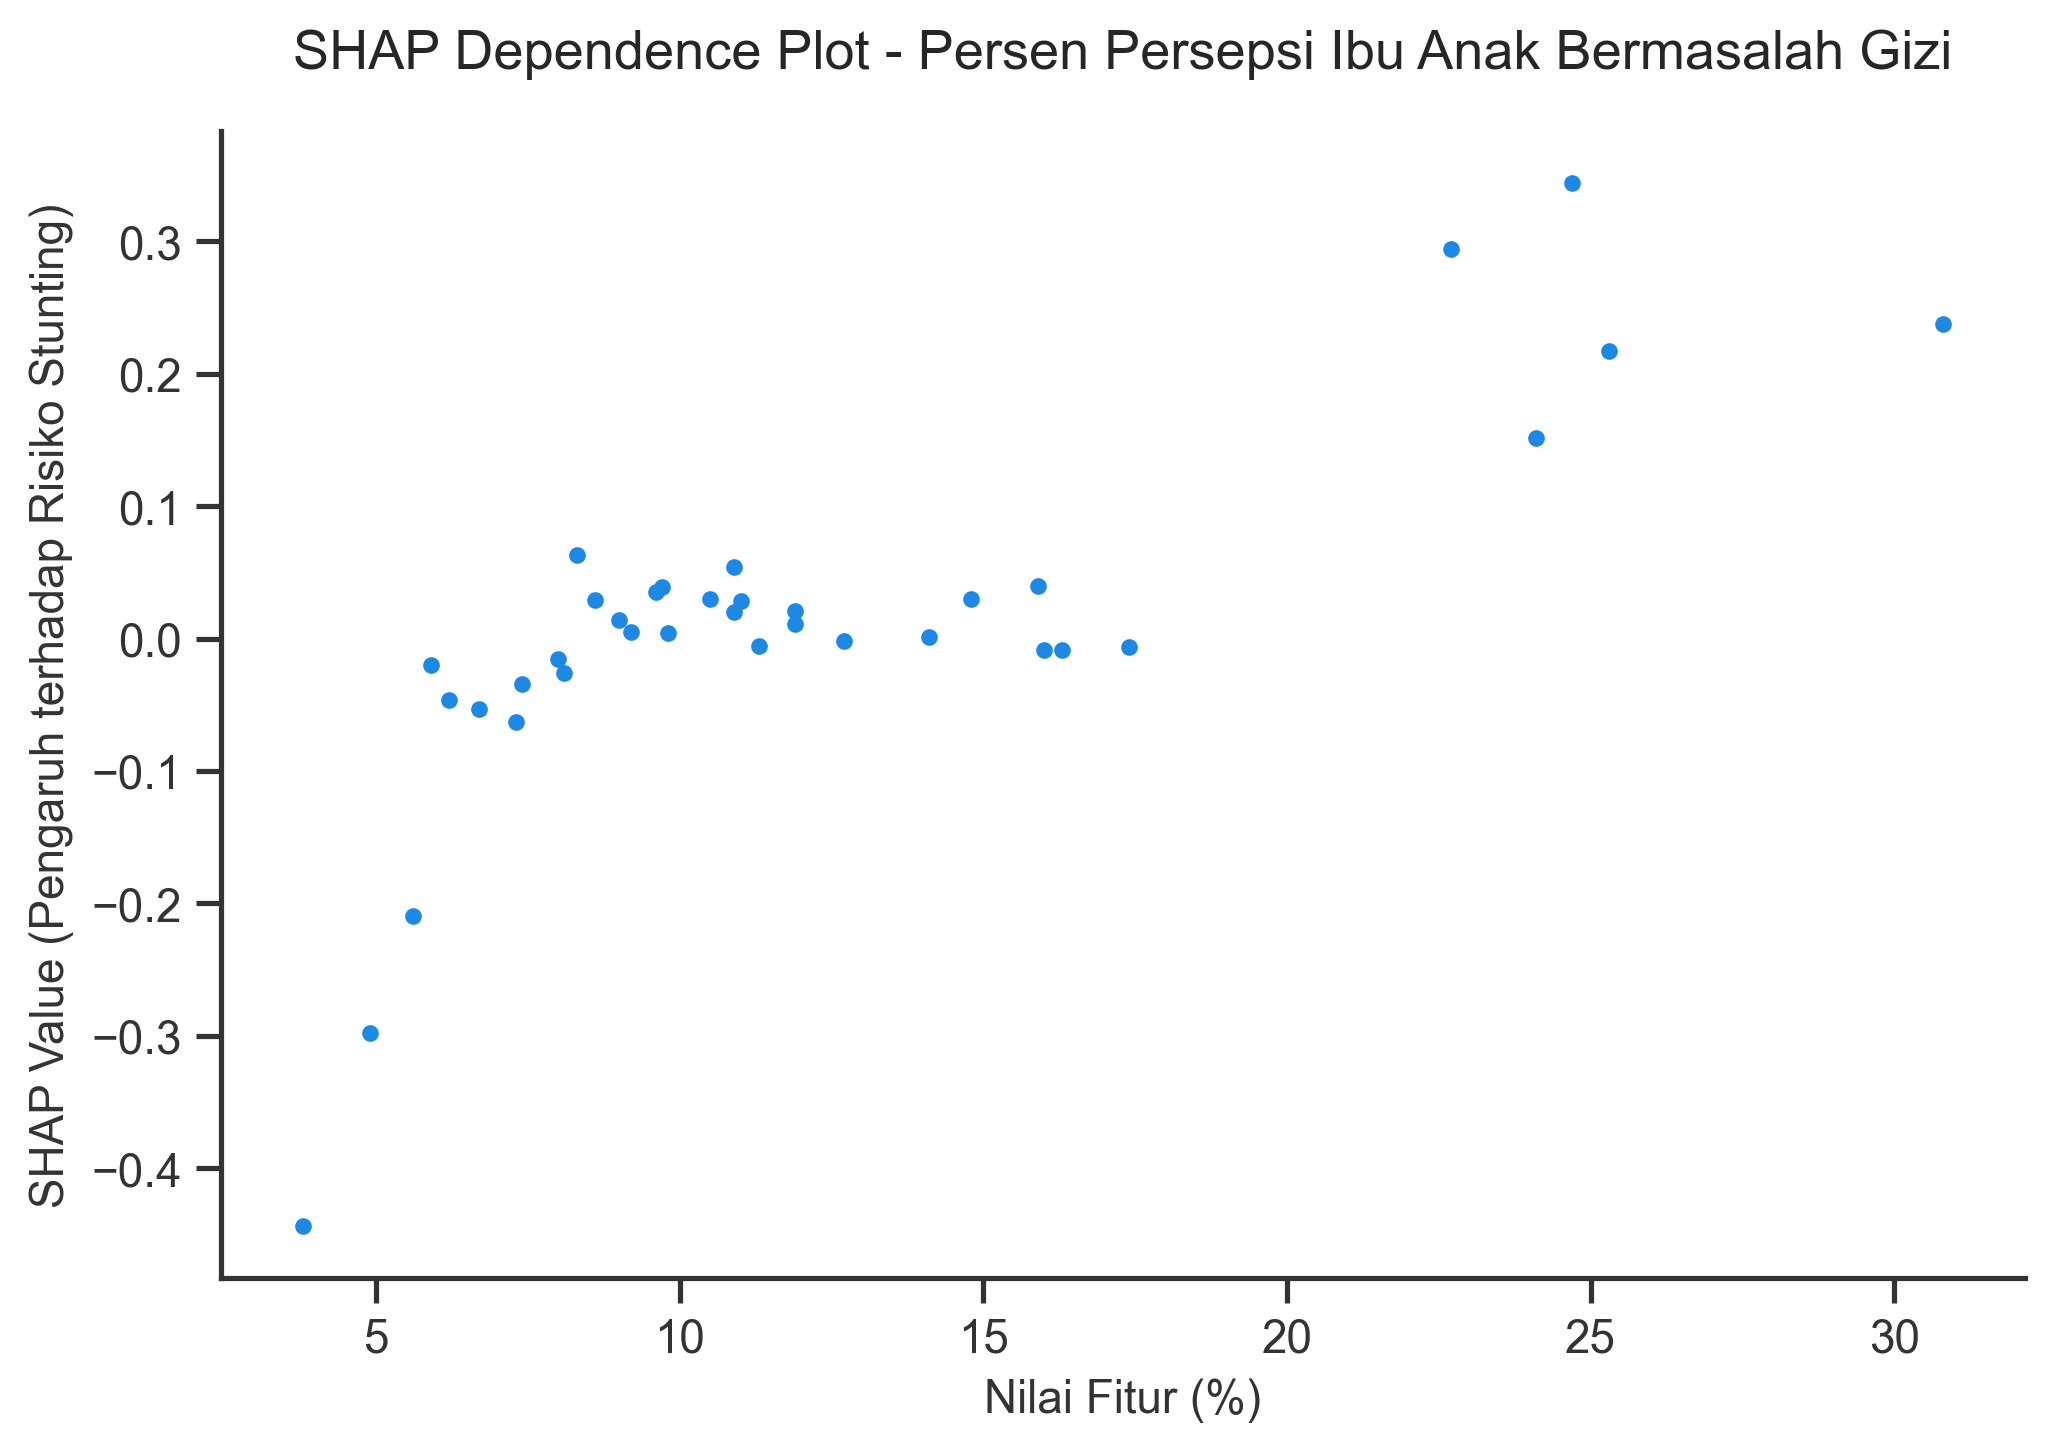
\includegraphics[width=0.48\textwidth]{figure/hasil_dependence_plot/dependence_persen_persepsi_ibu_anak_bermasalah_gizi.png}
\end{figure}

\newpage
\begin{figure}[H]
    \centering
    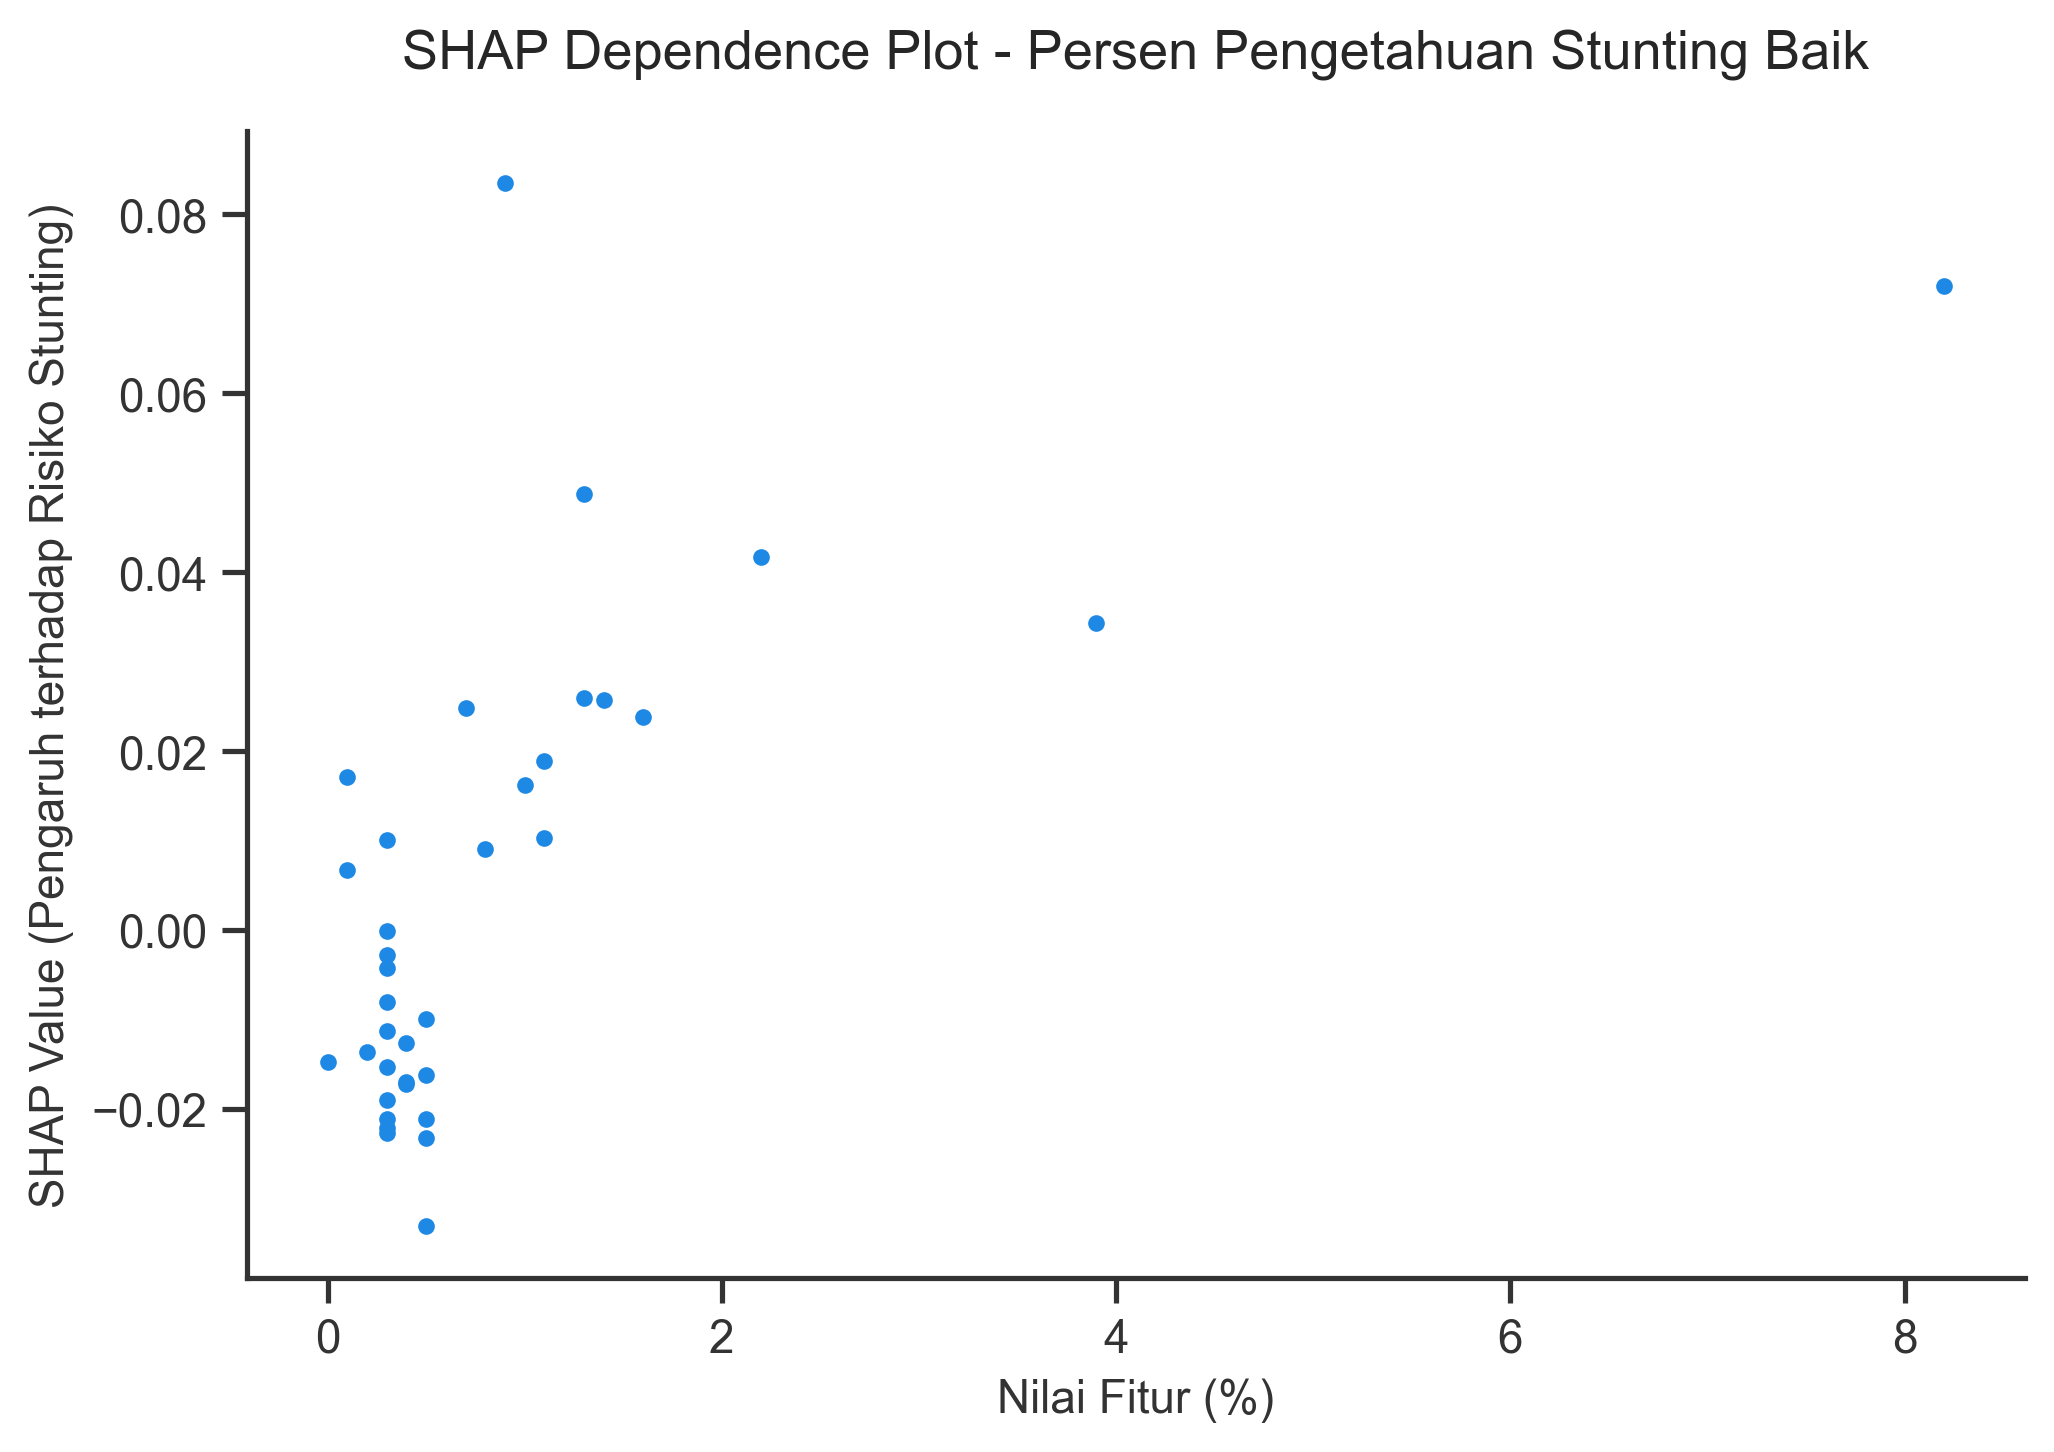
\includegraphics[width=0.48\textwidth]{figure/hasil_dependence_plot/dependence_persen_pengetahuan_stunting_baik.png} \hfill
    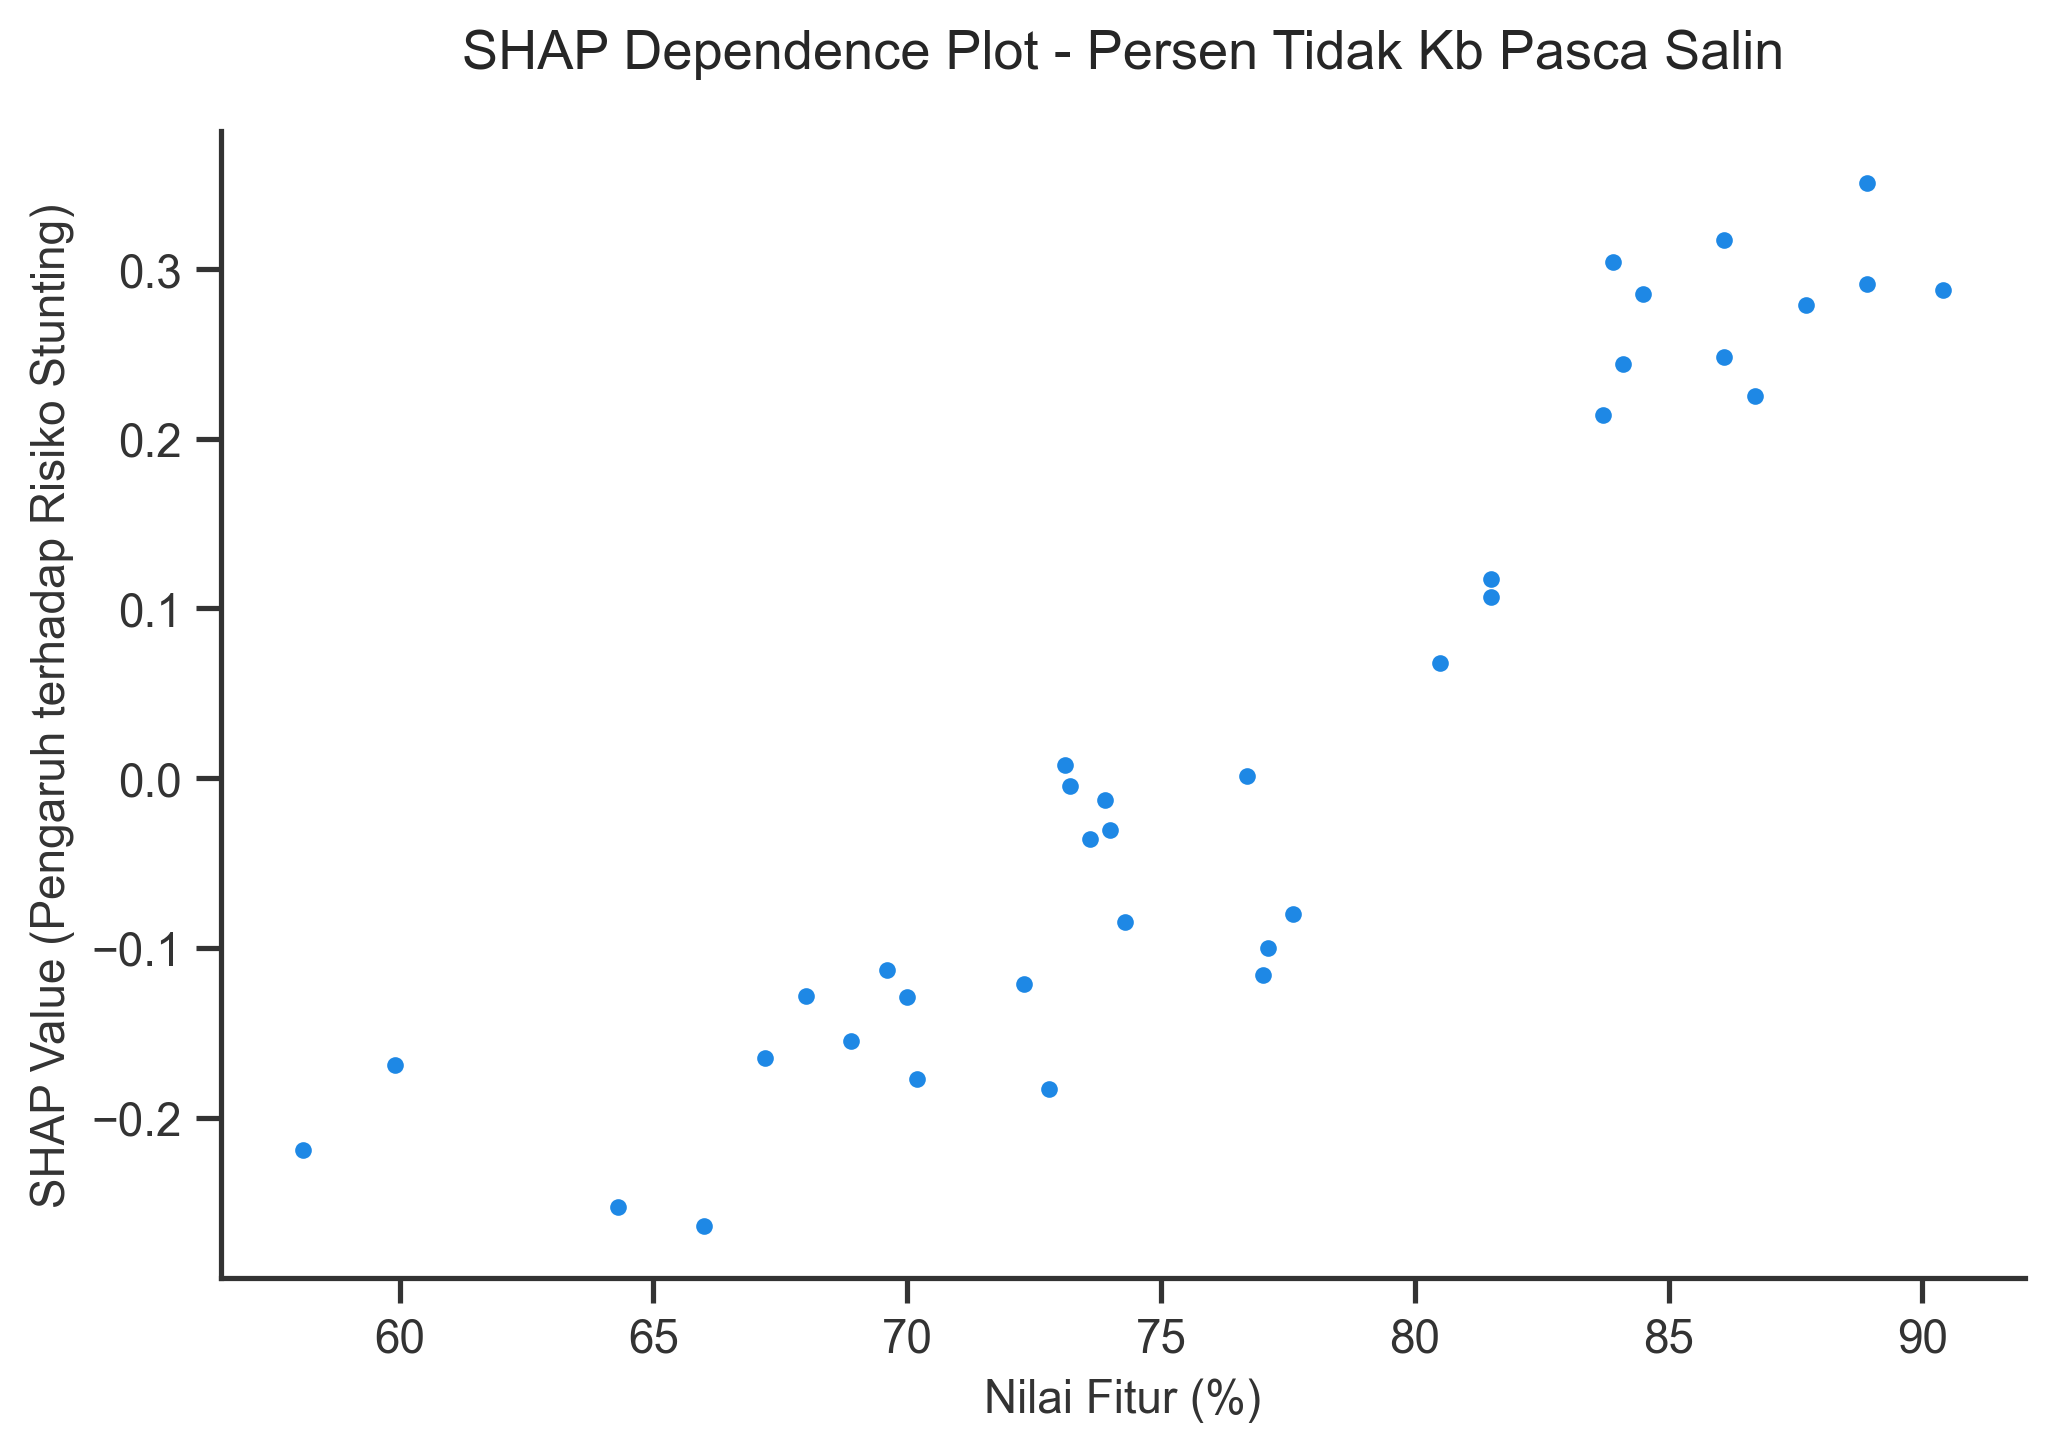
\includegraphics[width=0.48\textwidth]{figure/hasil_dependence_plot/dependence_persen_tidak_kb_pasca_salin.png} \\ \vspace{0.2cm}
    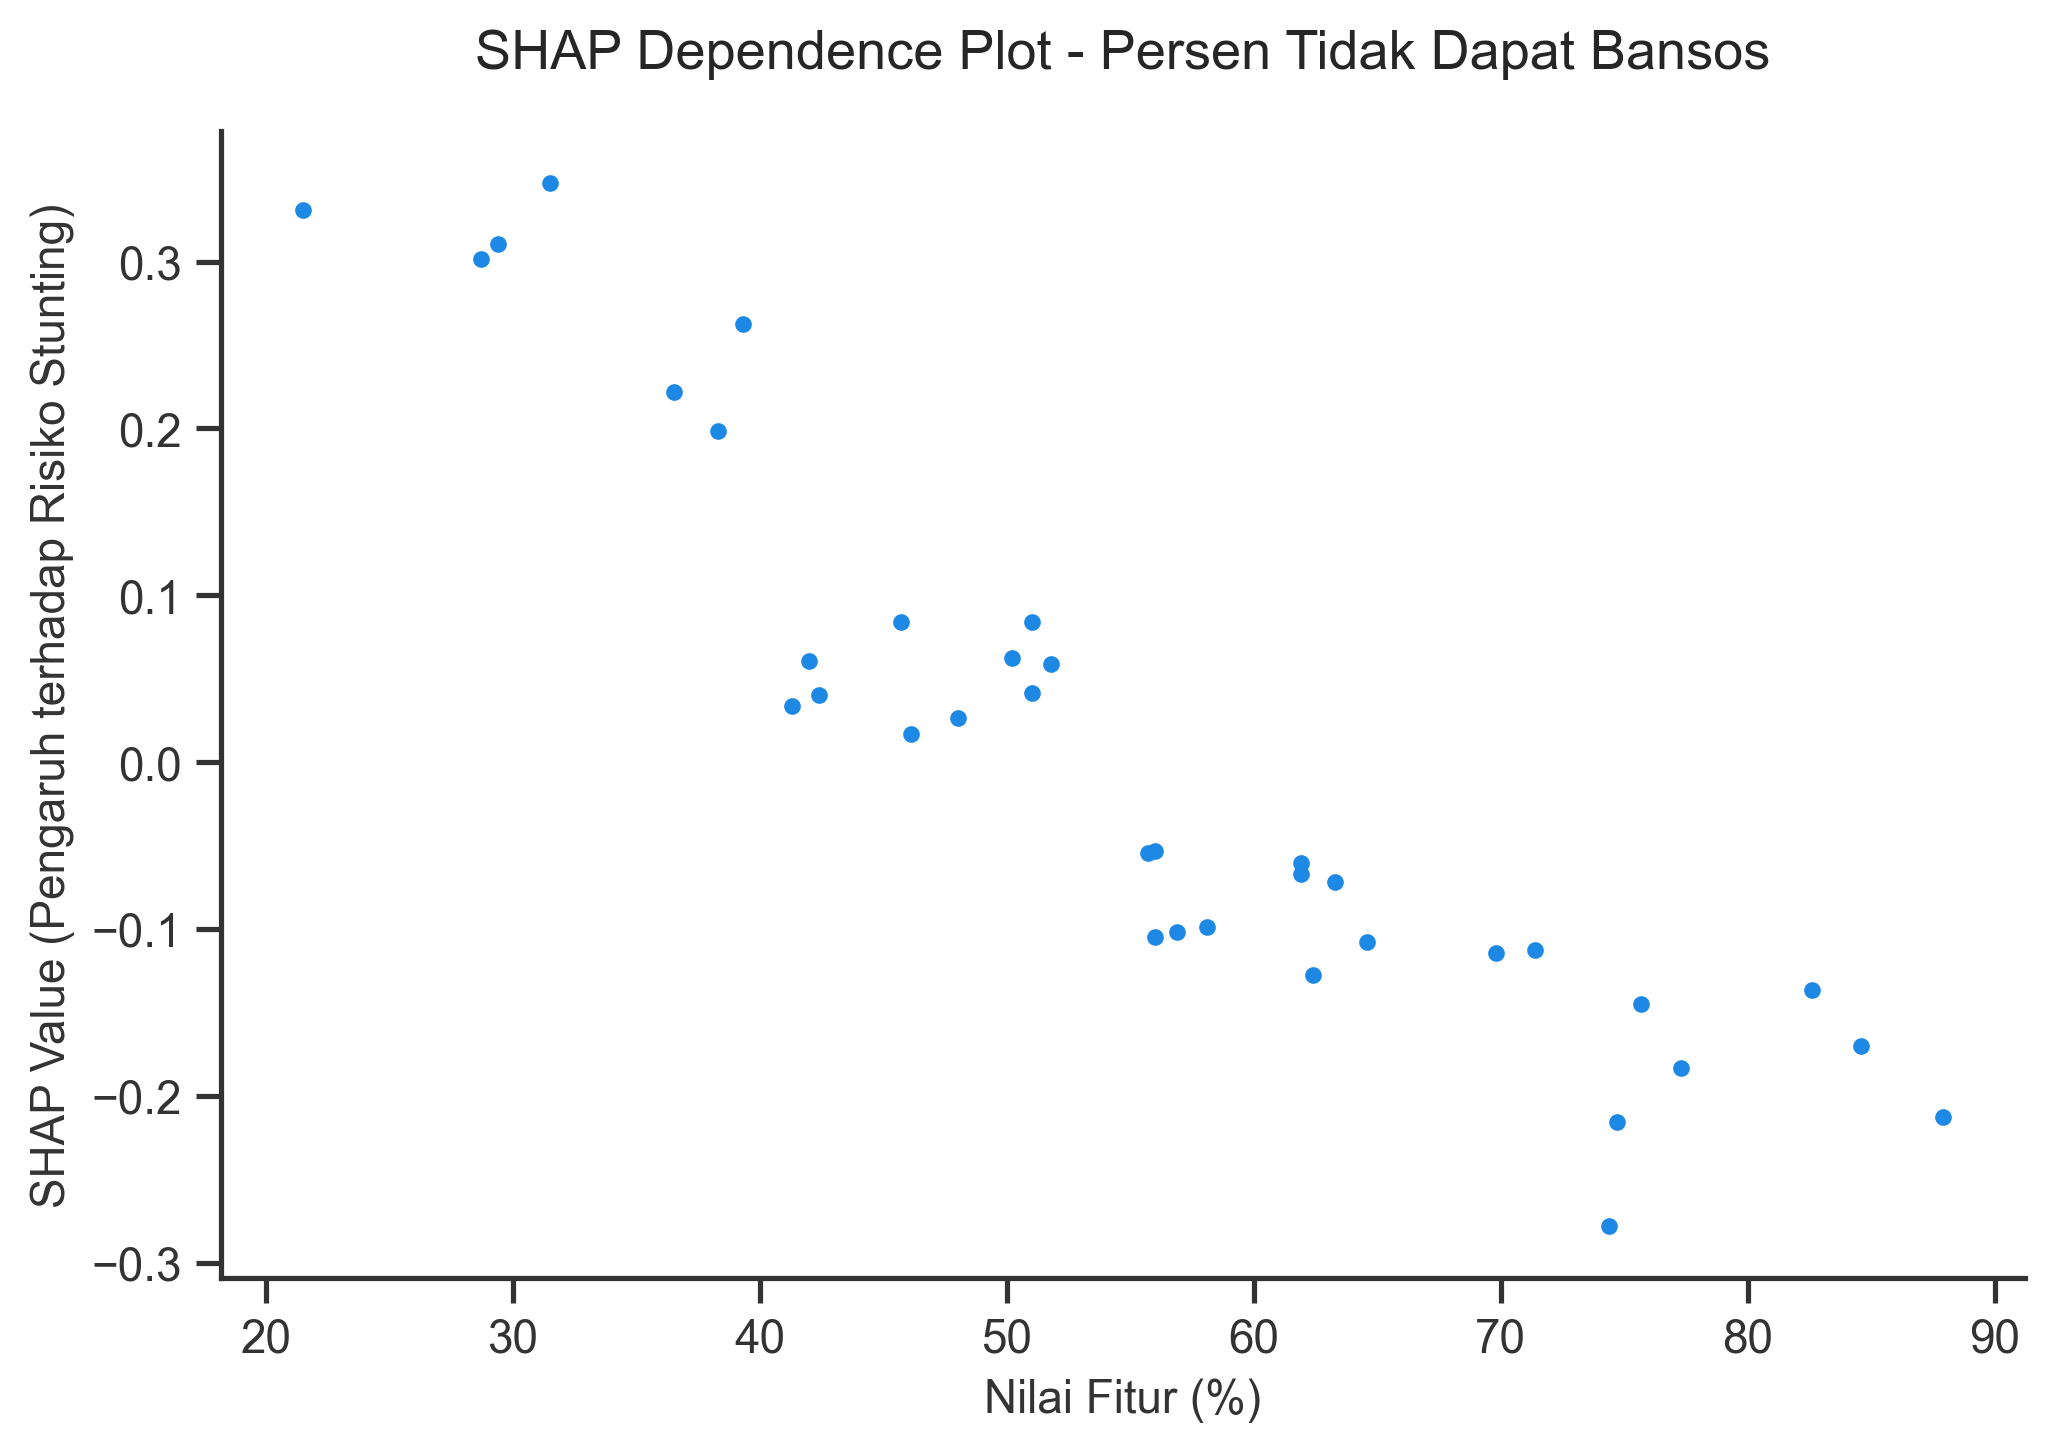
\includegraphics[width=0.48\textwidth]{figure/hasil_dependence_plot/dependence_persen_tidak_dapat_bansos.png} \hfill
    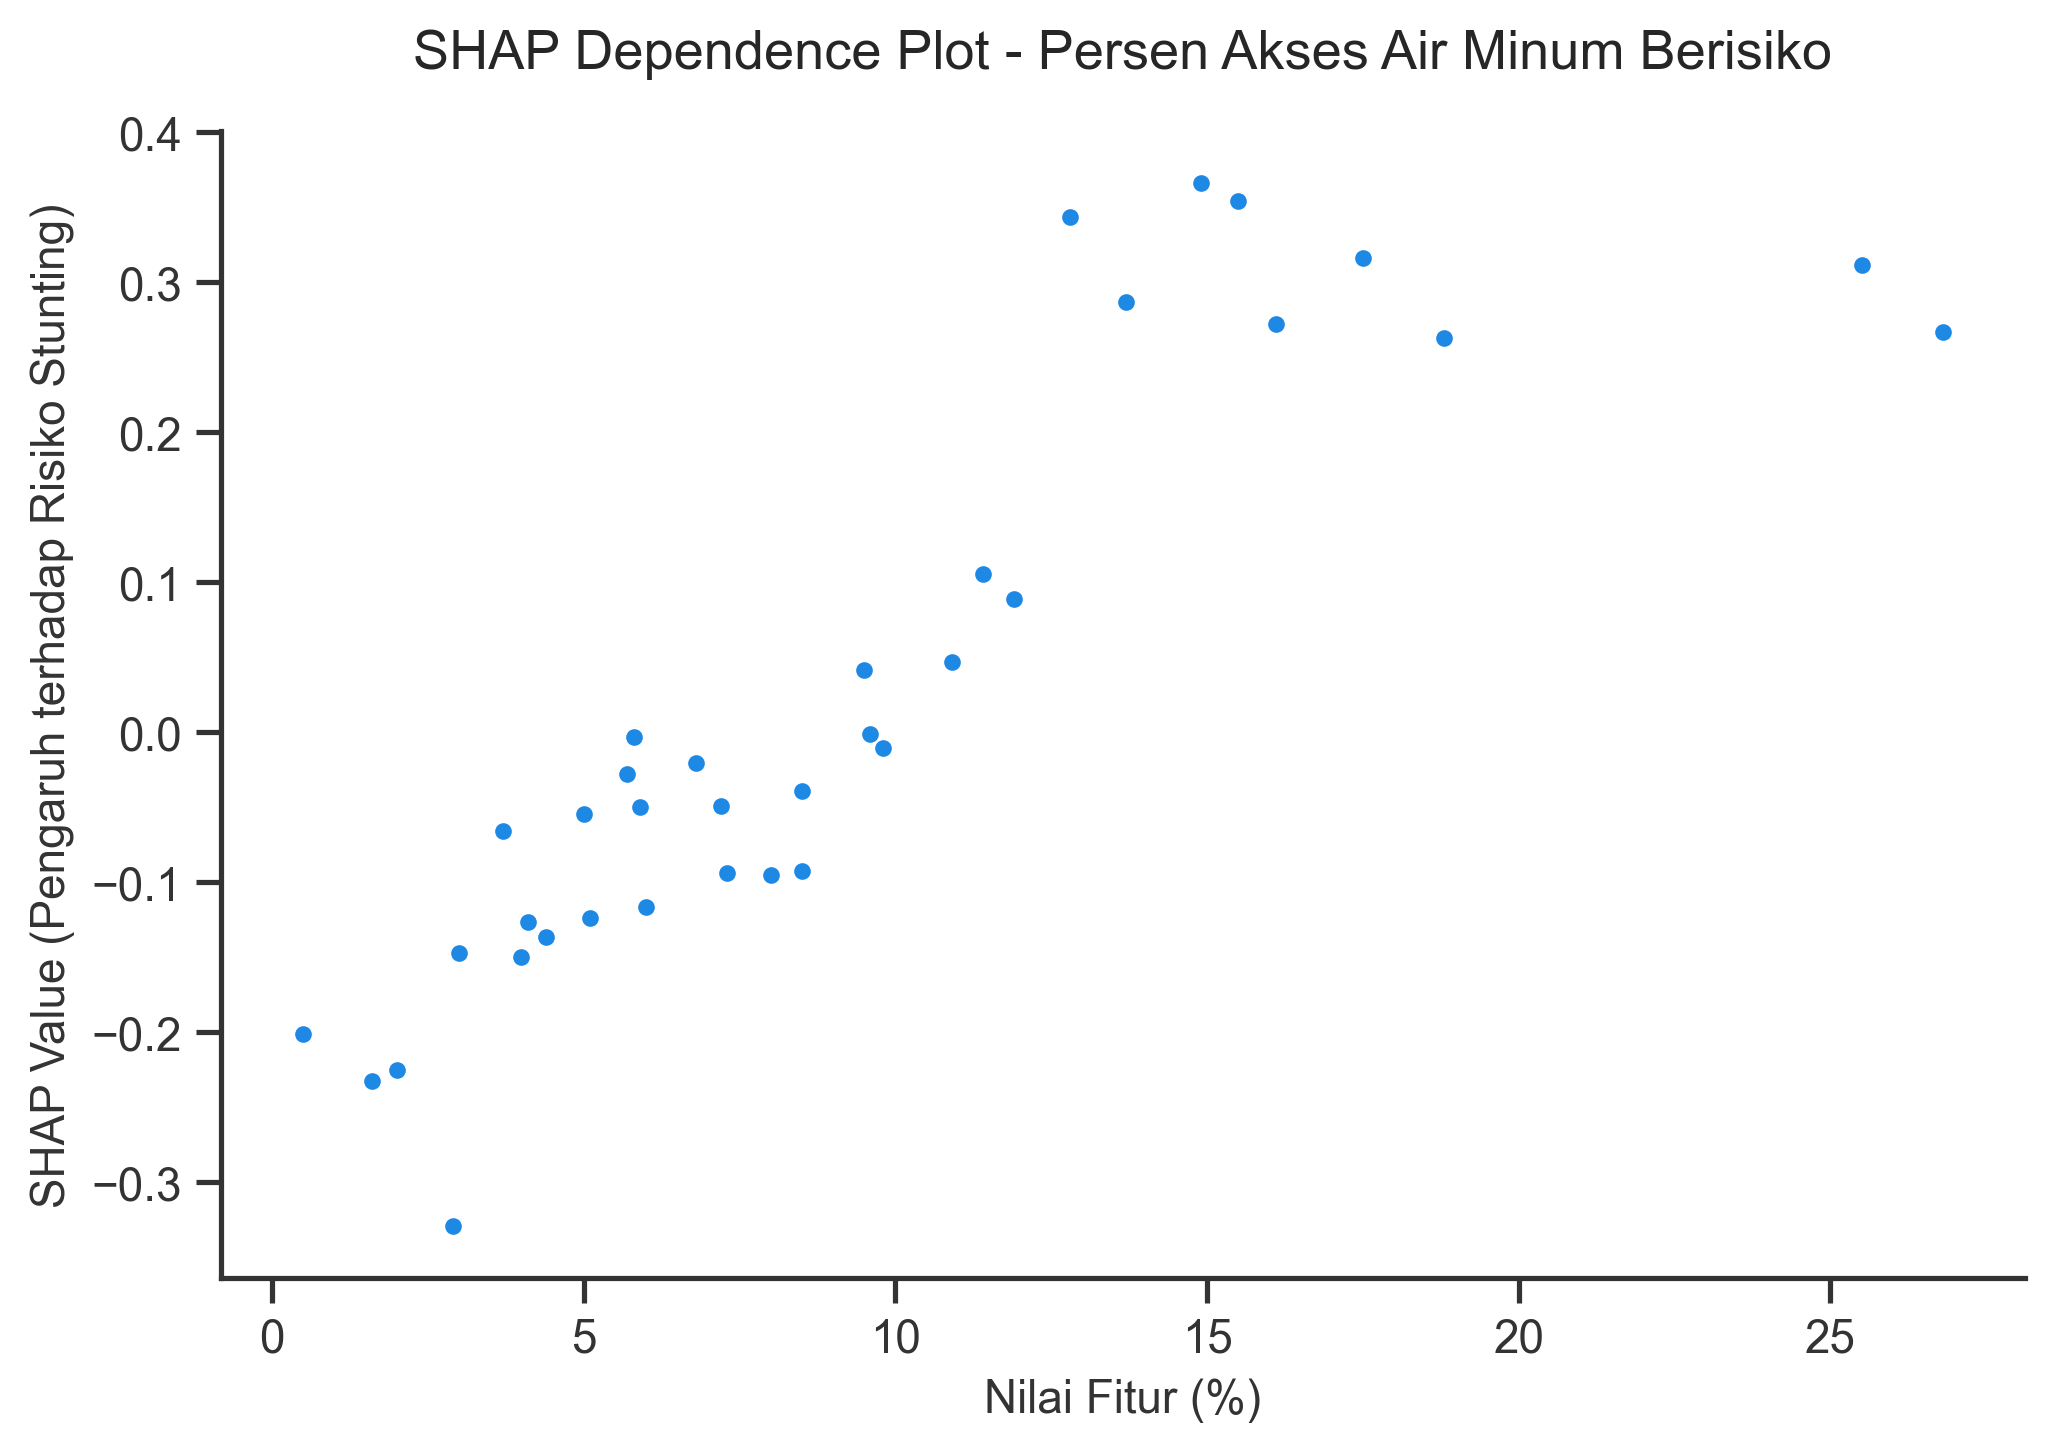
\includegraphics[width=0.48\textwidth]{figure/hasil_dependence_plot/dependence_persen_akses_air_minum_berisiko.png} \\ \vspace{0.2cm}
    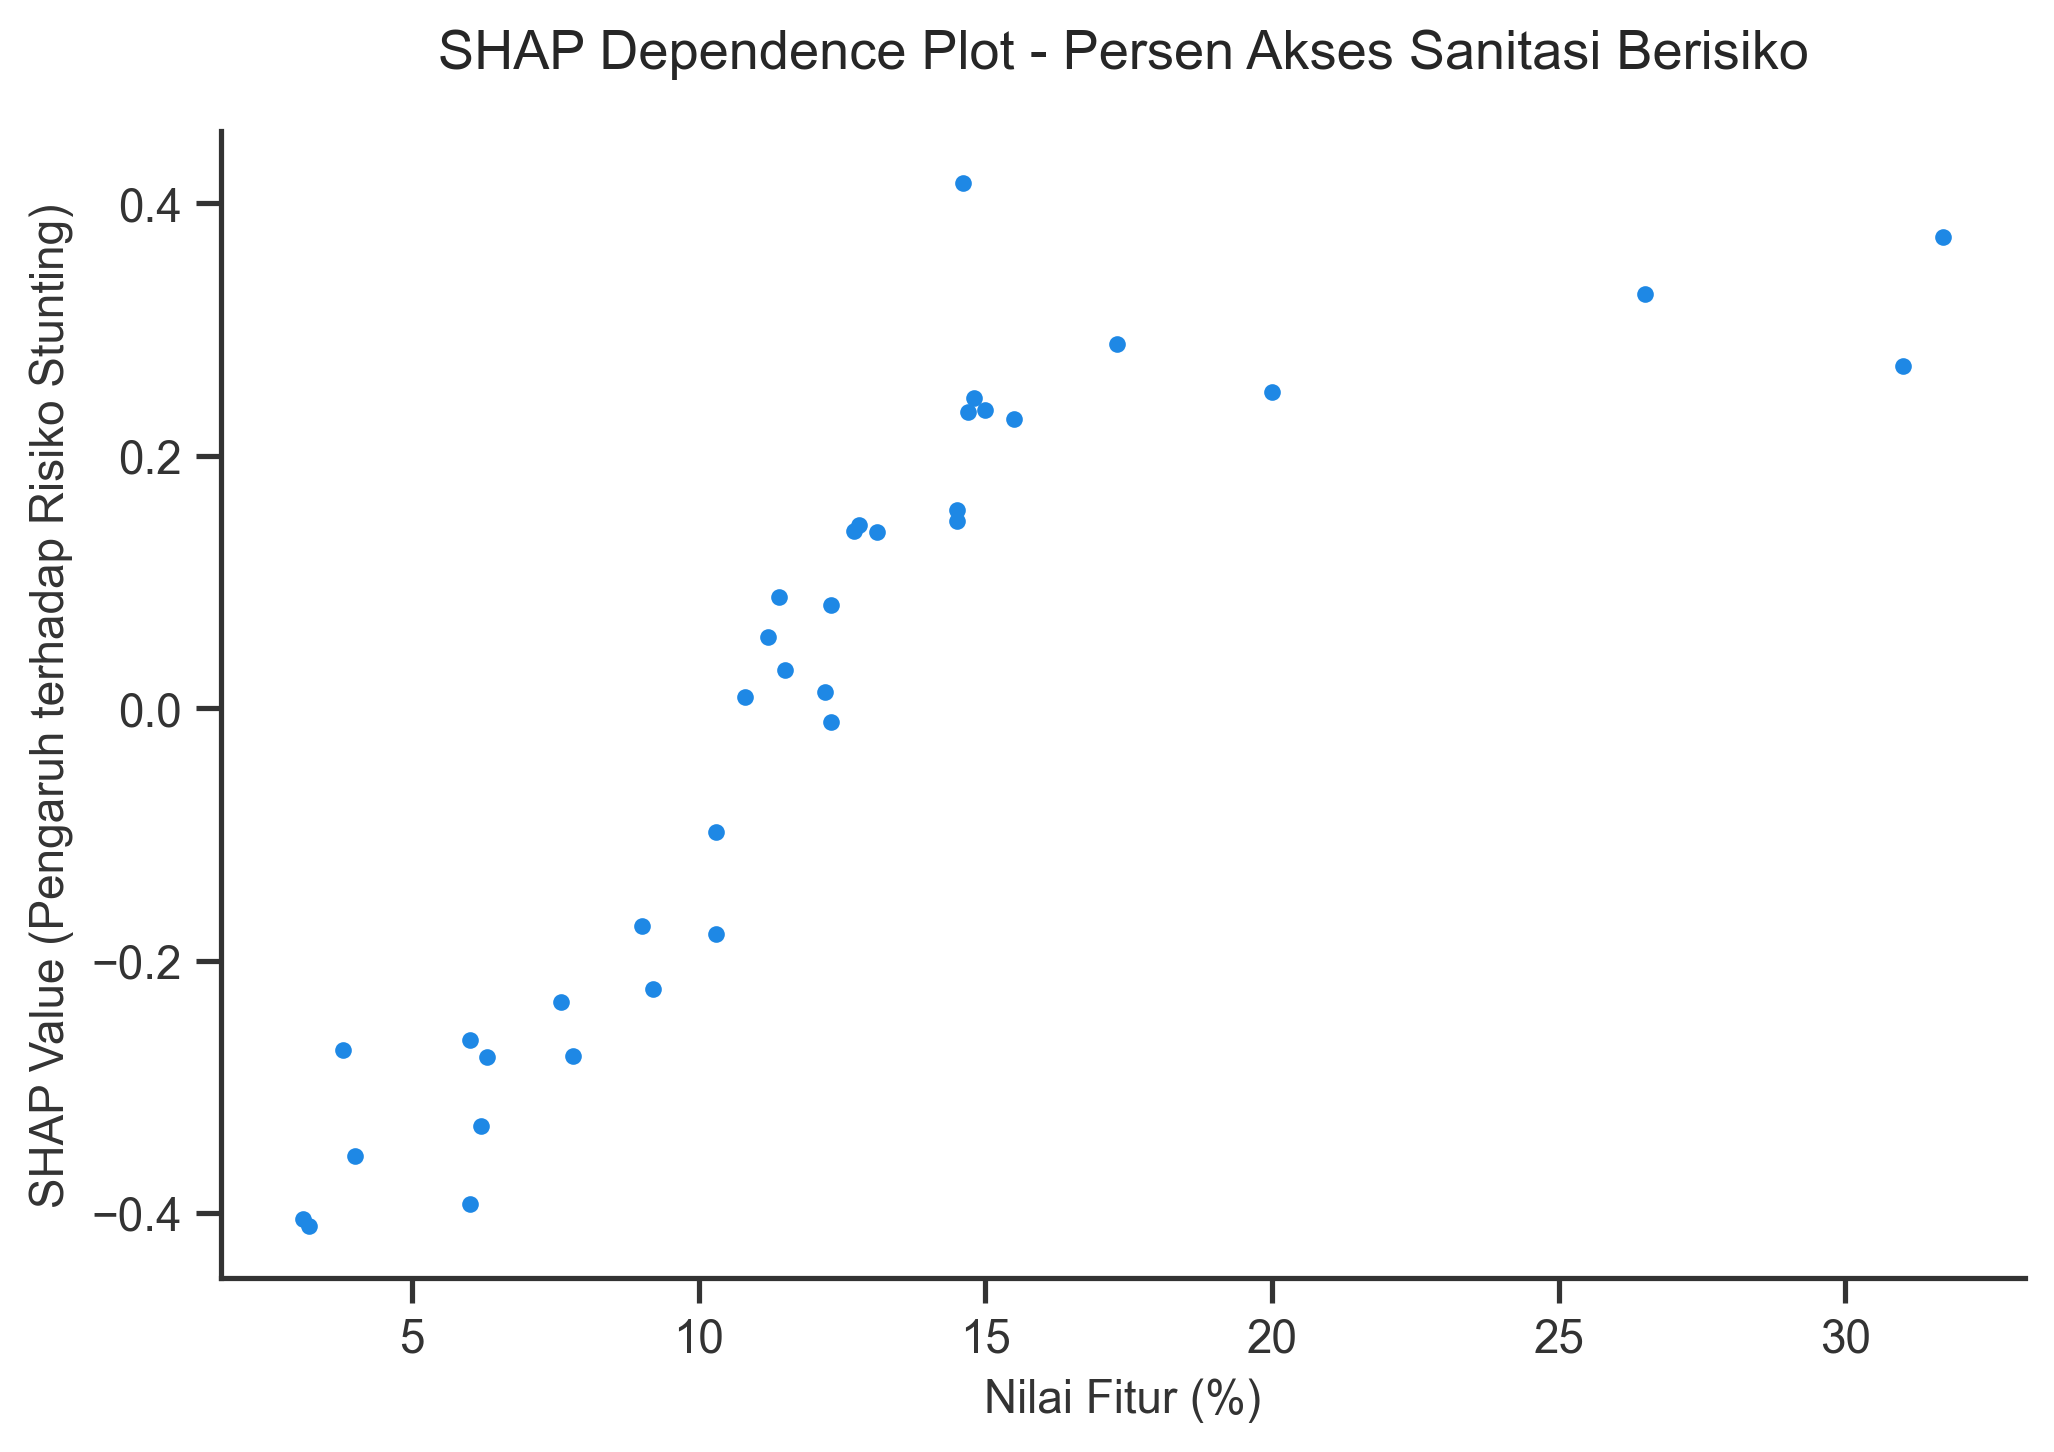
\includegraphics[width=0.48\textwidth]{figure/hasil_dependence_plot/dependence_persen_akses_sanitasi_berisiko.png} \hfill
    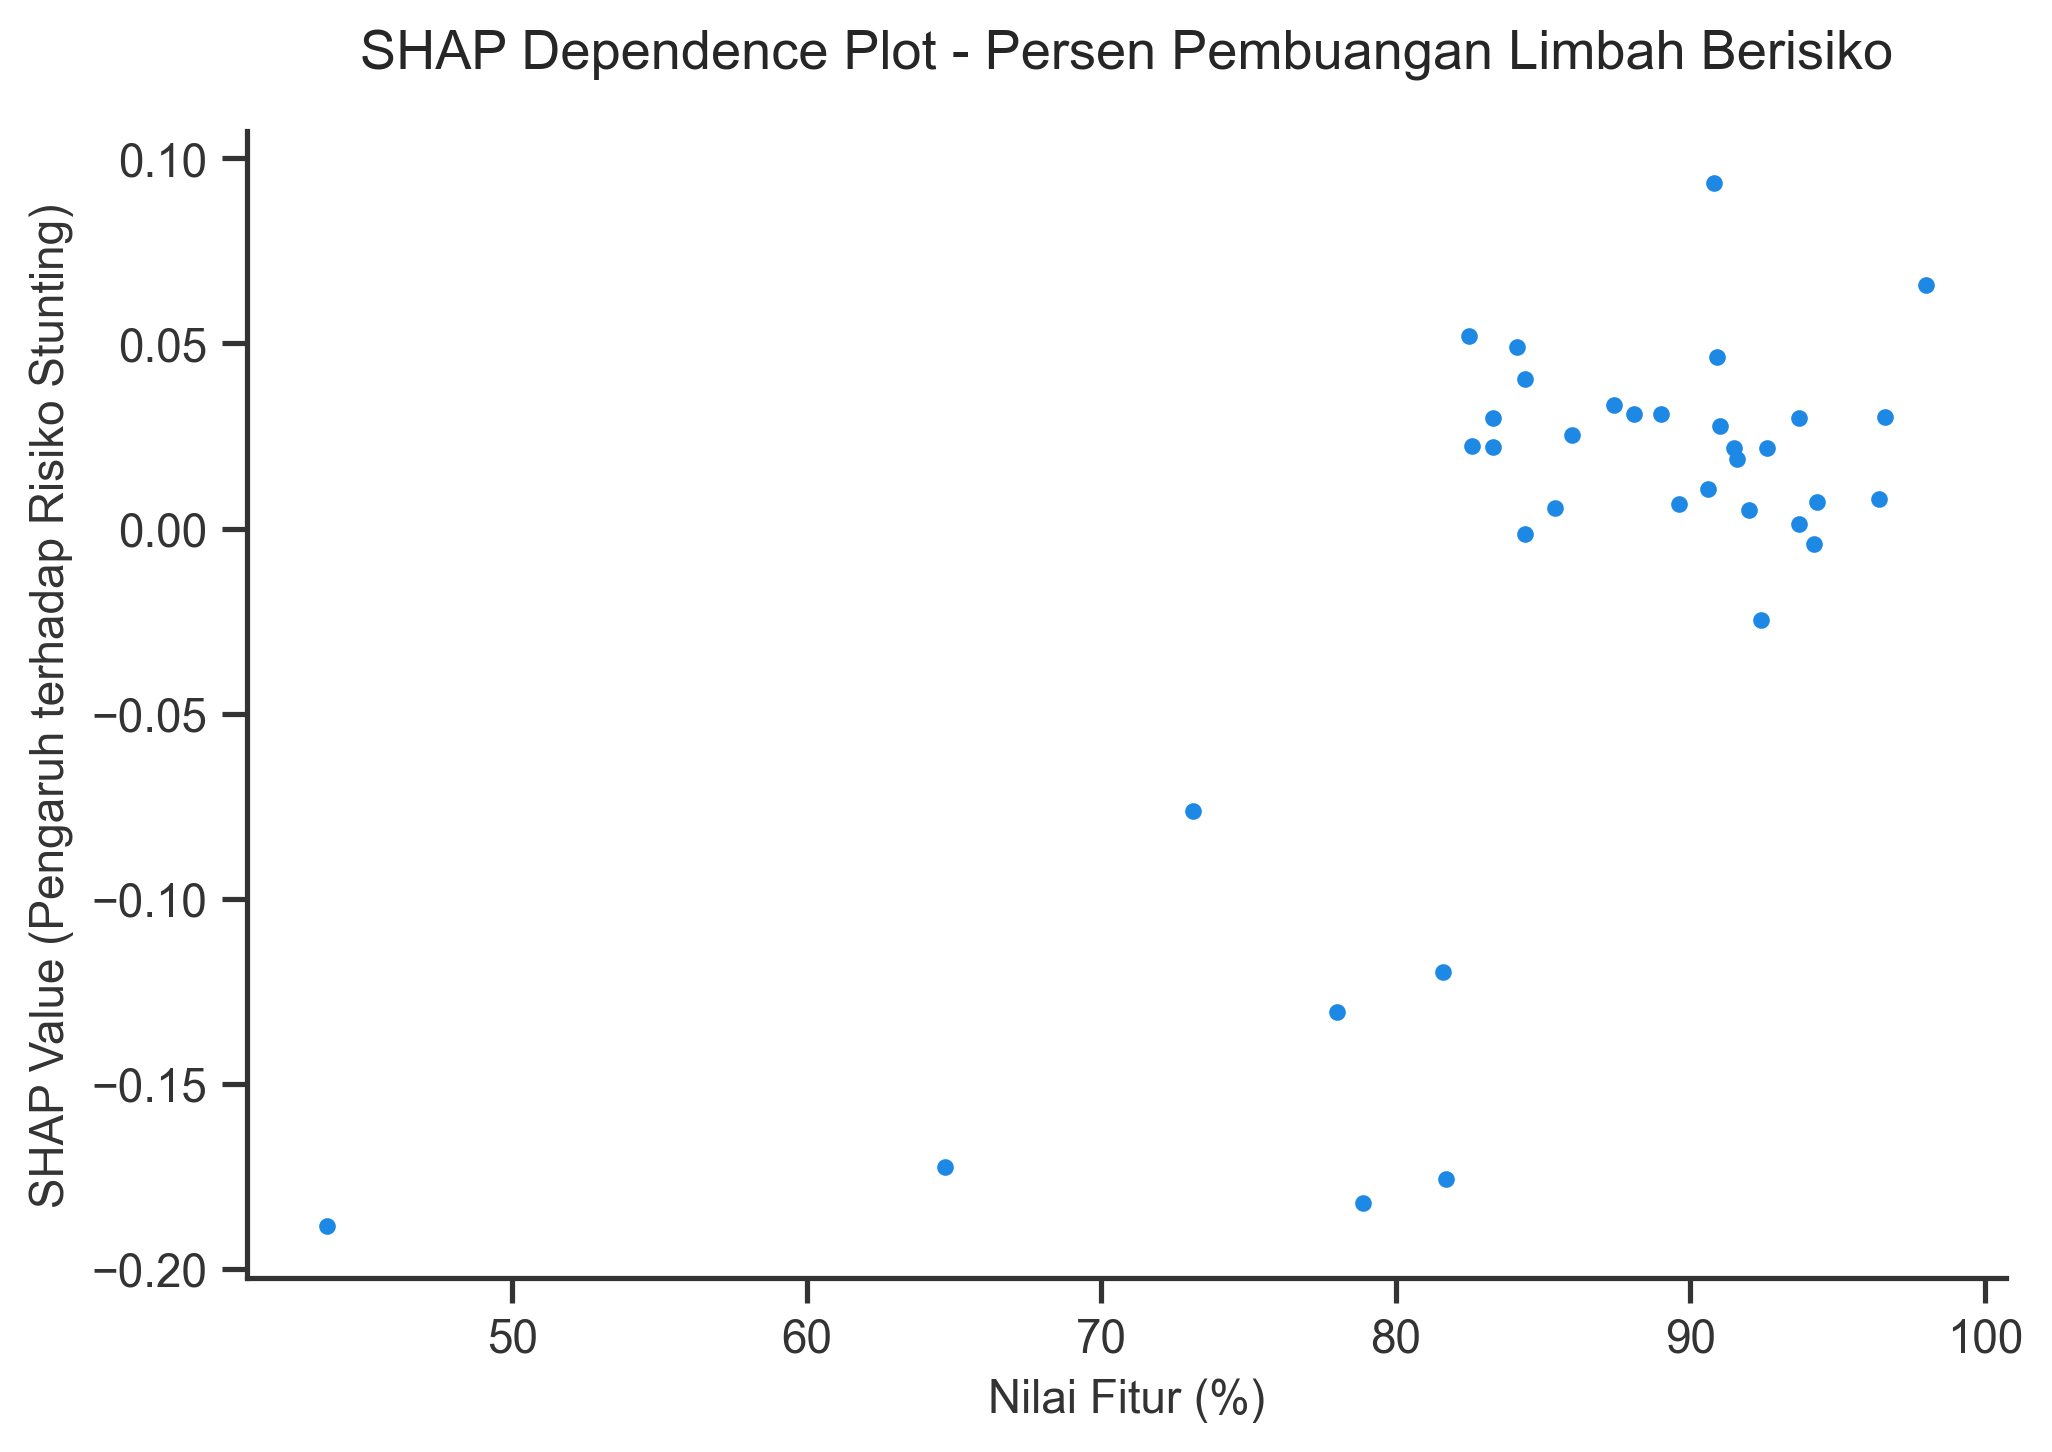
\includegraphics[width=0.48\textwidth]{figure/hasil_dependence_plot/dependence_persen_pembuangan_limbah_berisiko.png}
\end{figure}

% --- LAMPIRAN VI ---
\newpage
\refstepcounter{chapter} 
\addcontentsline{toc}{section}{Lampiran \thechapter\ Grafik Kontribusi Fitur Per Provinsi (\textit{SHAP Waterfall Plot})}
\noindent{\large Lampiran \thechapter\ Grafik Kontribusi Fitur Per Provinsi (\textit{SHAP Waterfall Plot})} \par
\vspace{0.5cm}

\begin{center}
    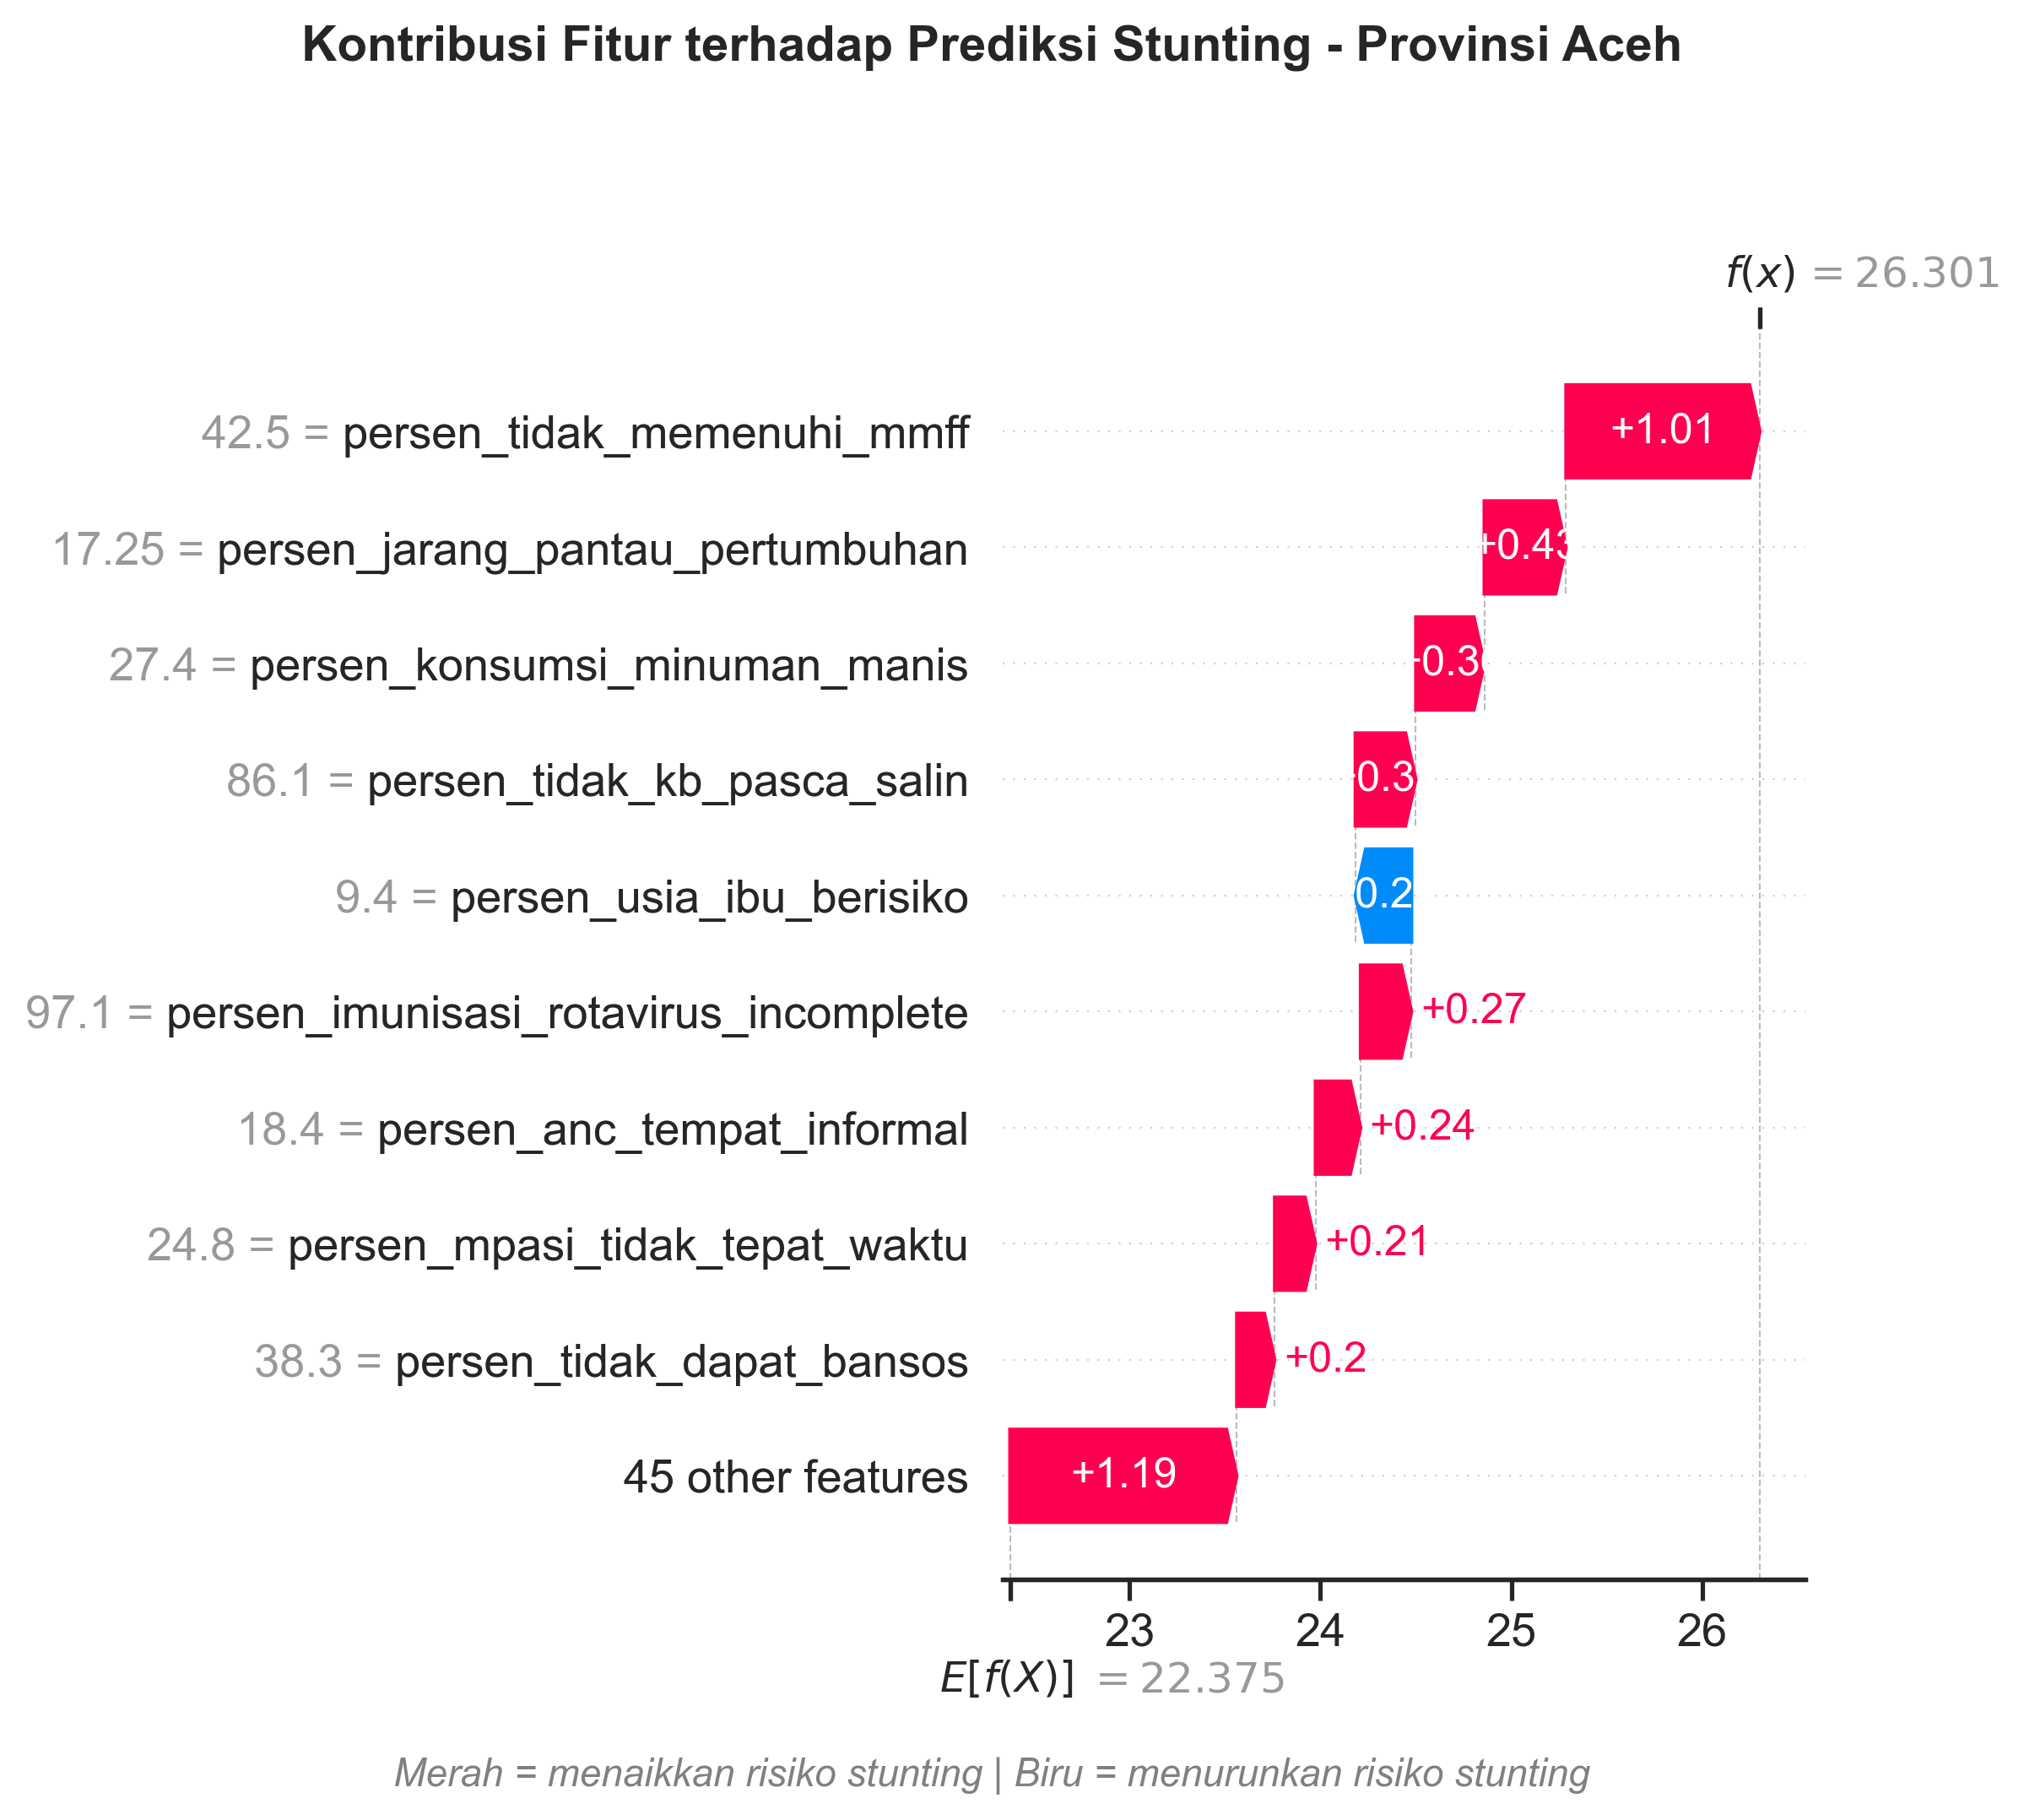
\includegraphics[width=0.48\textwidth]{figure/hasil_waterfall_stunting/waterfall_Aceh.png} \hfill
    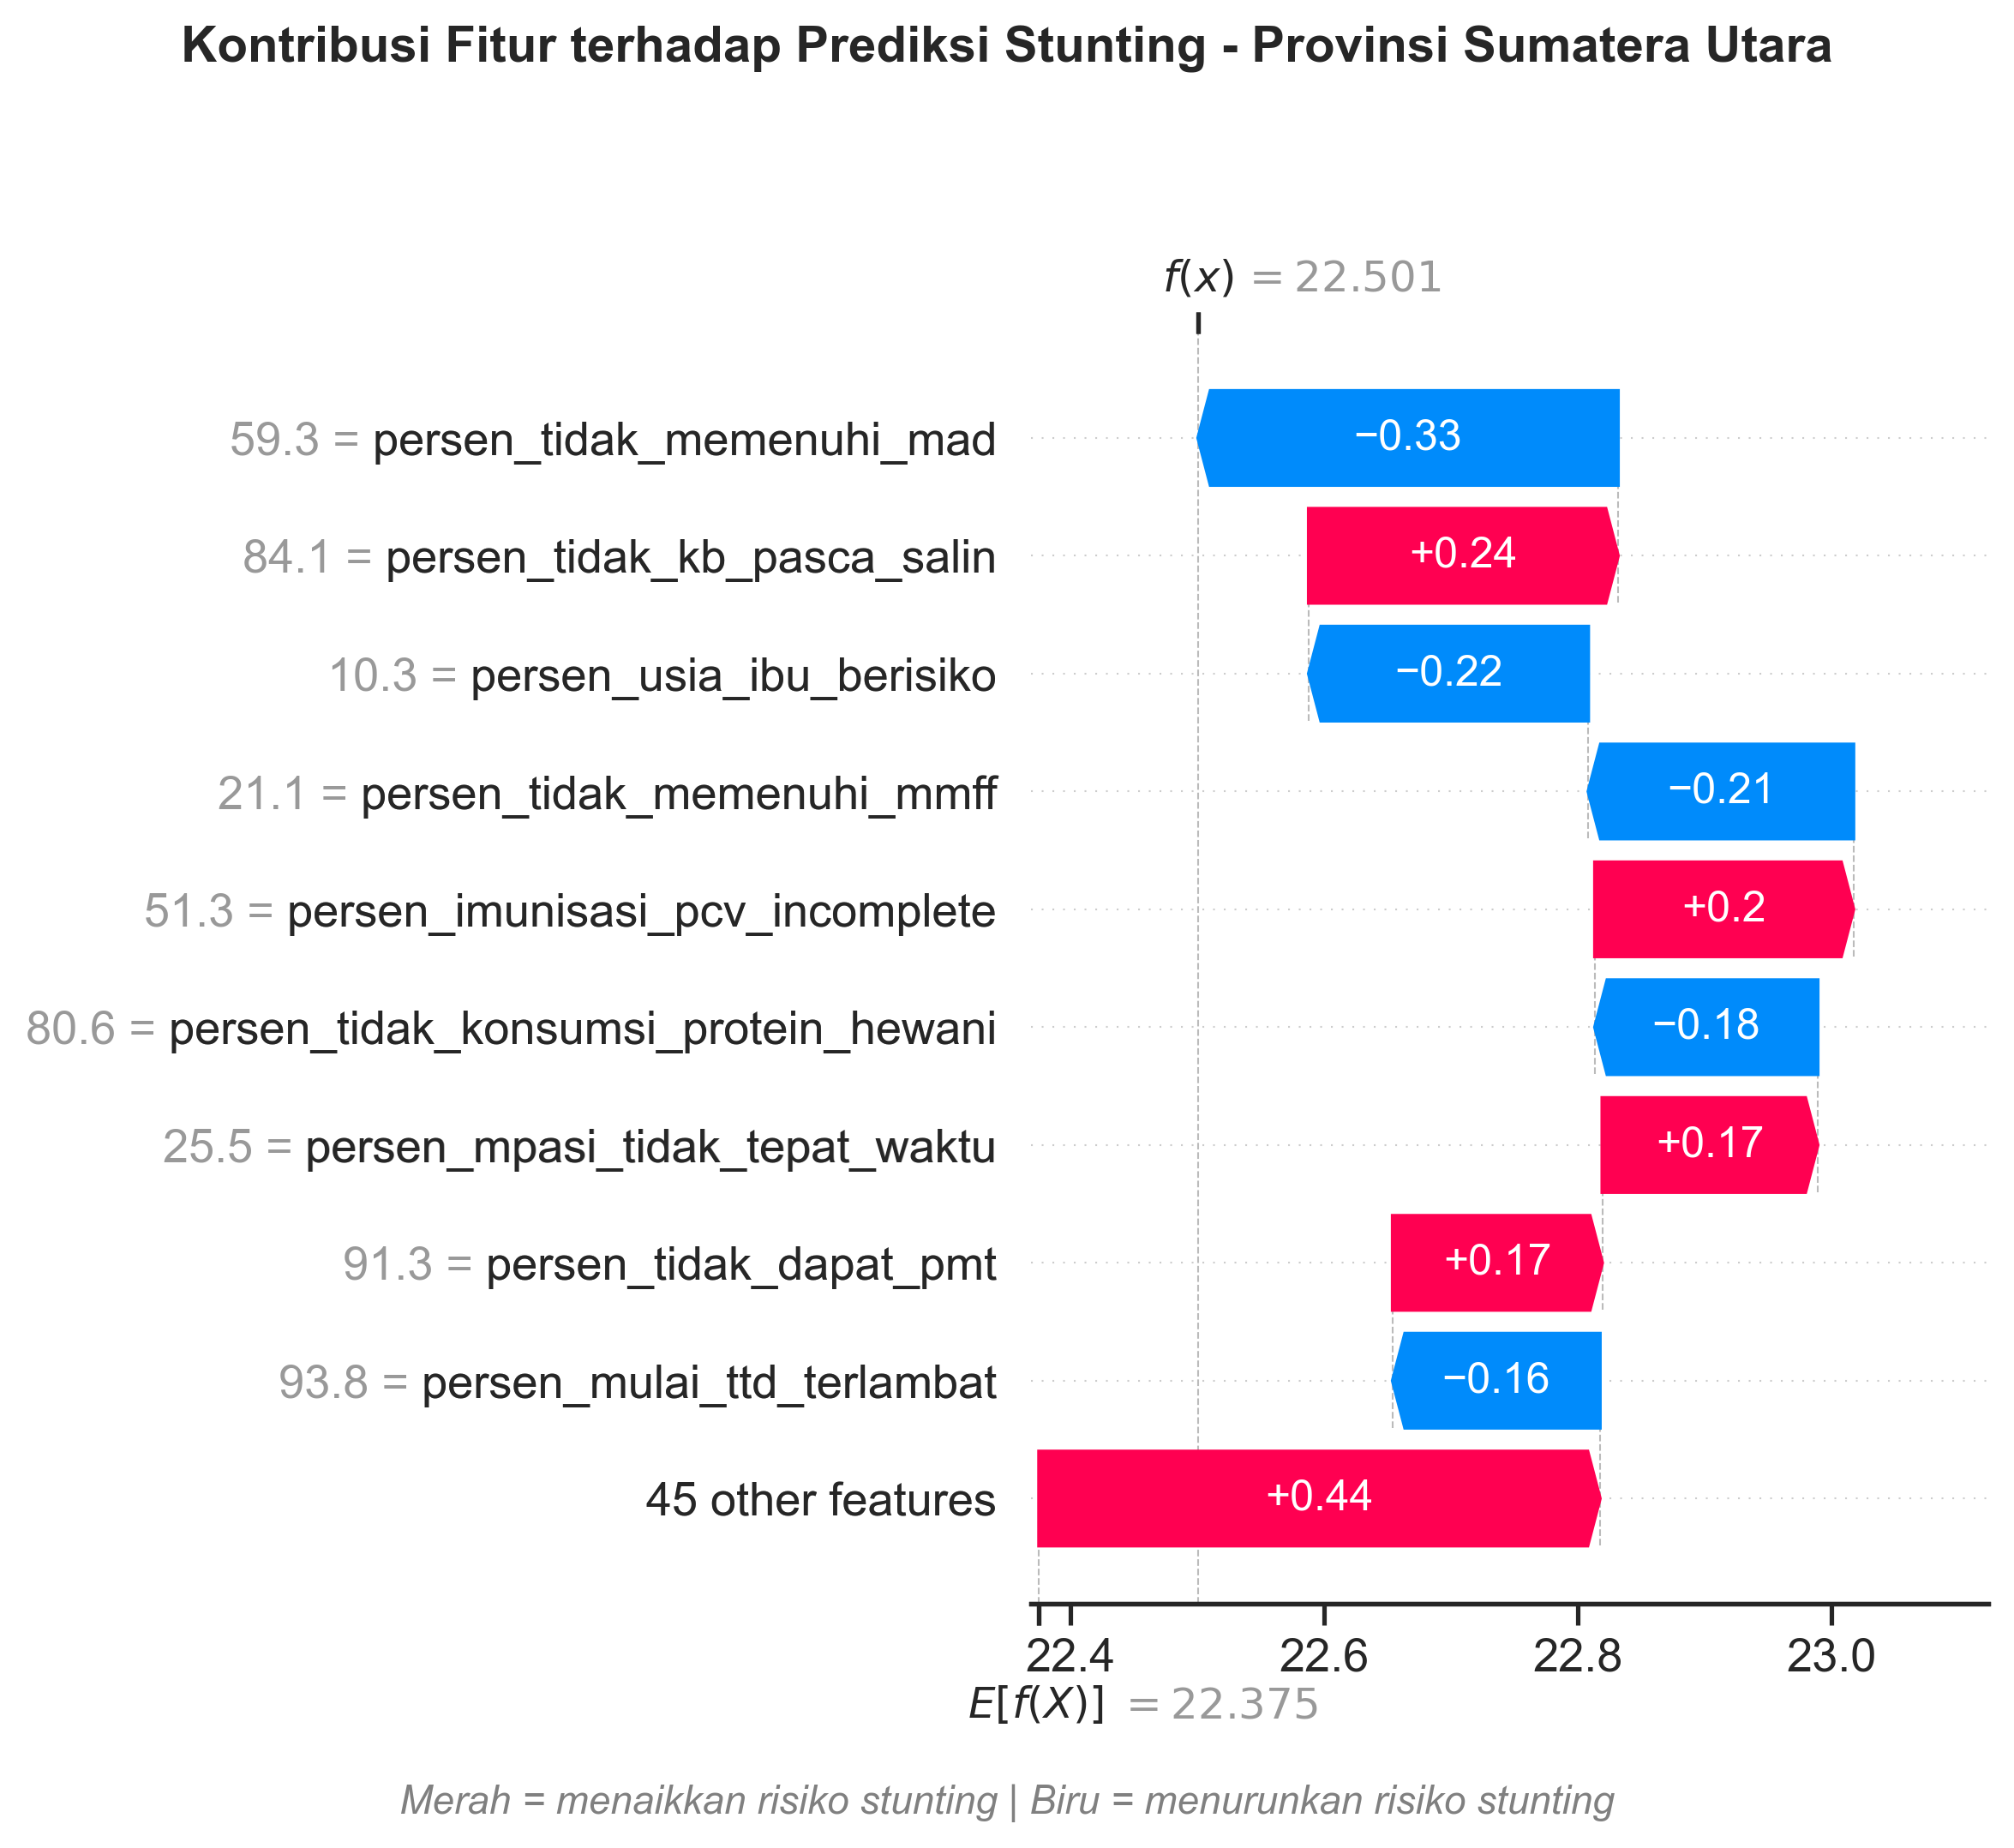
\includegraphics[width=0.48\textwidth]{figure/hasil_waterfall_stunting/waterfall_Sumatera_Utara.png} \\ \vspace{0.5cm}
    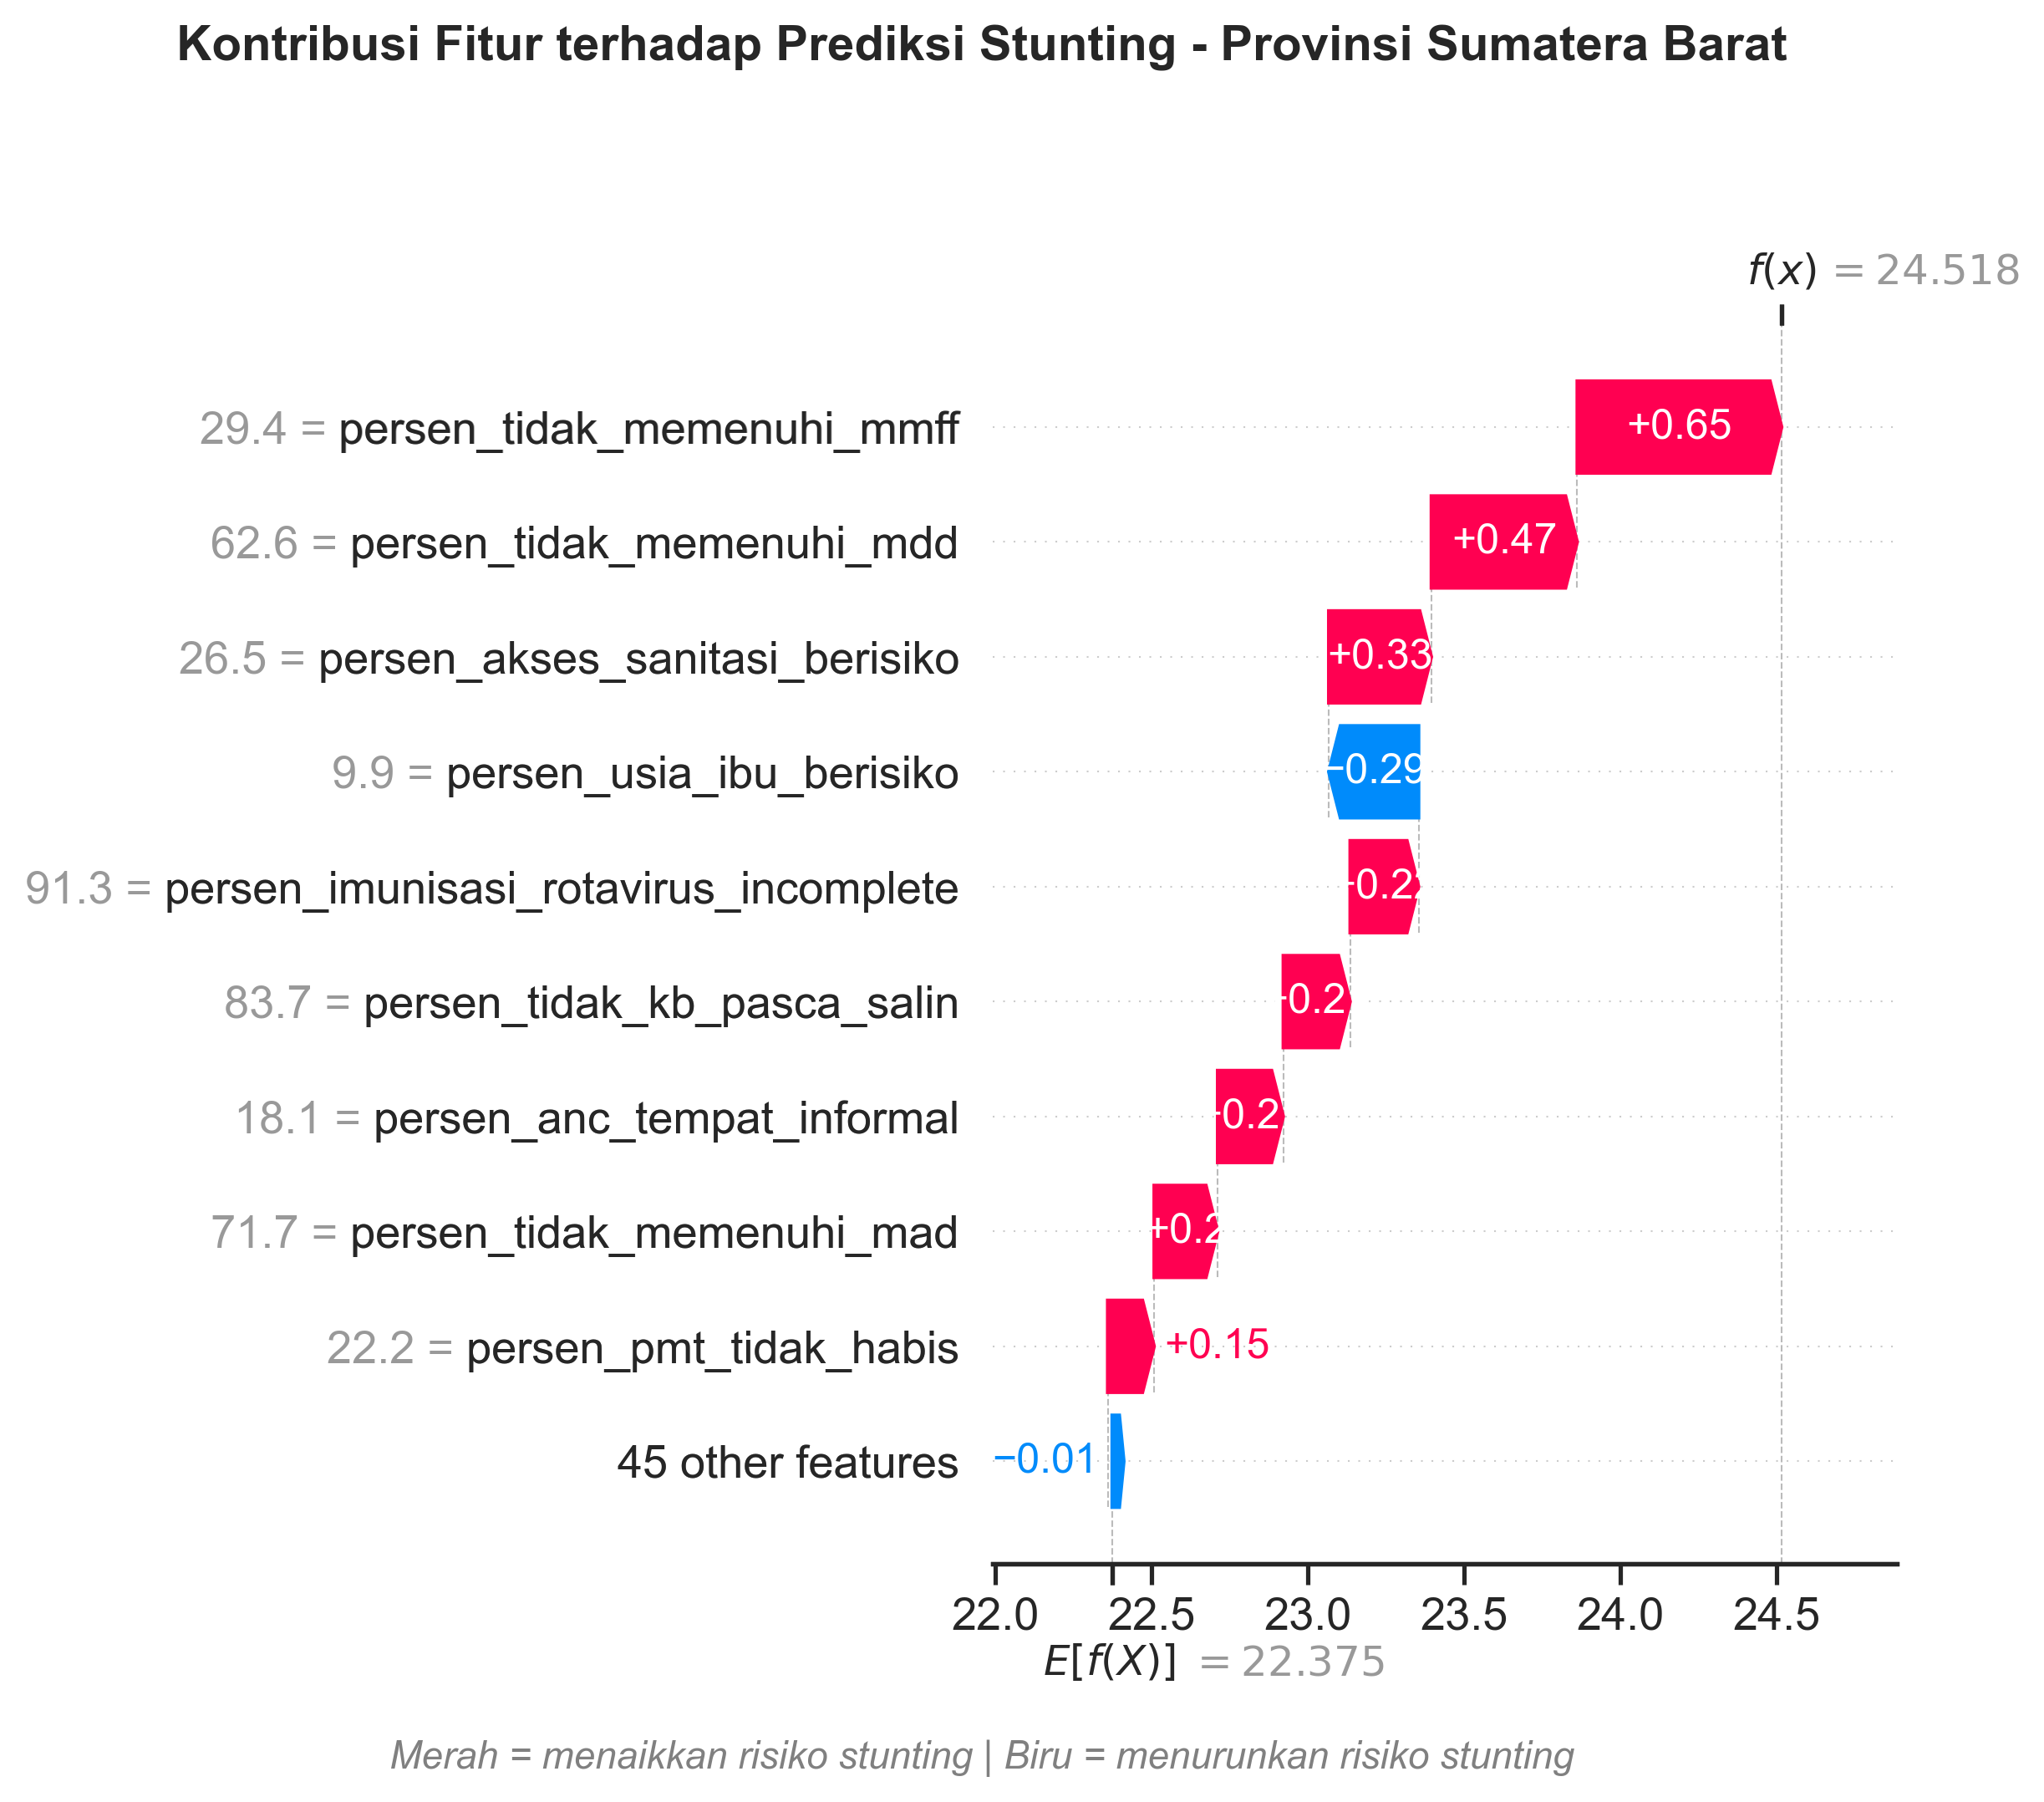
\includegraphics[width=0.48\textwidth]{figure/hasil_waterfall_stunting/waterfall_Sumatera_Barat.png} \hfill
    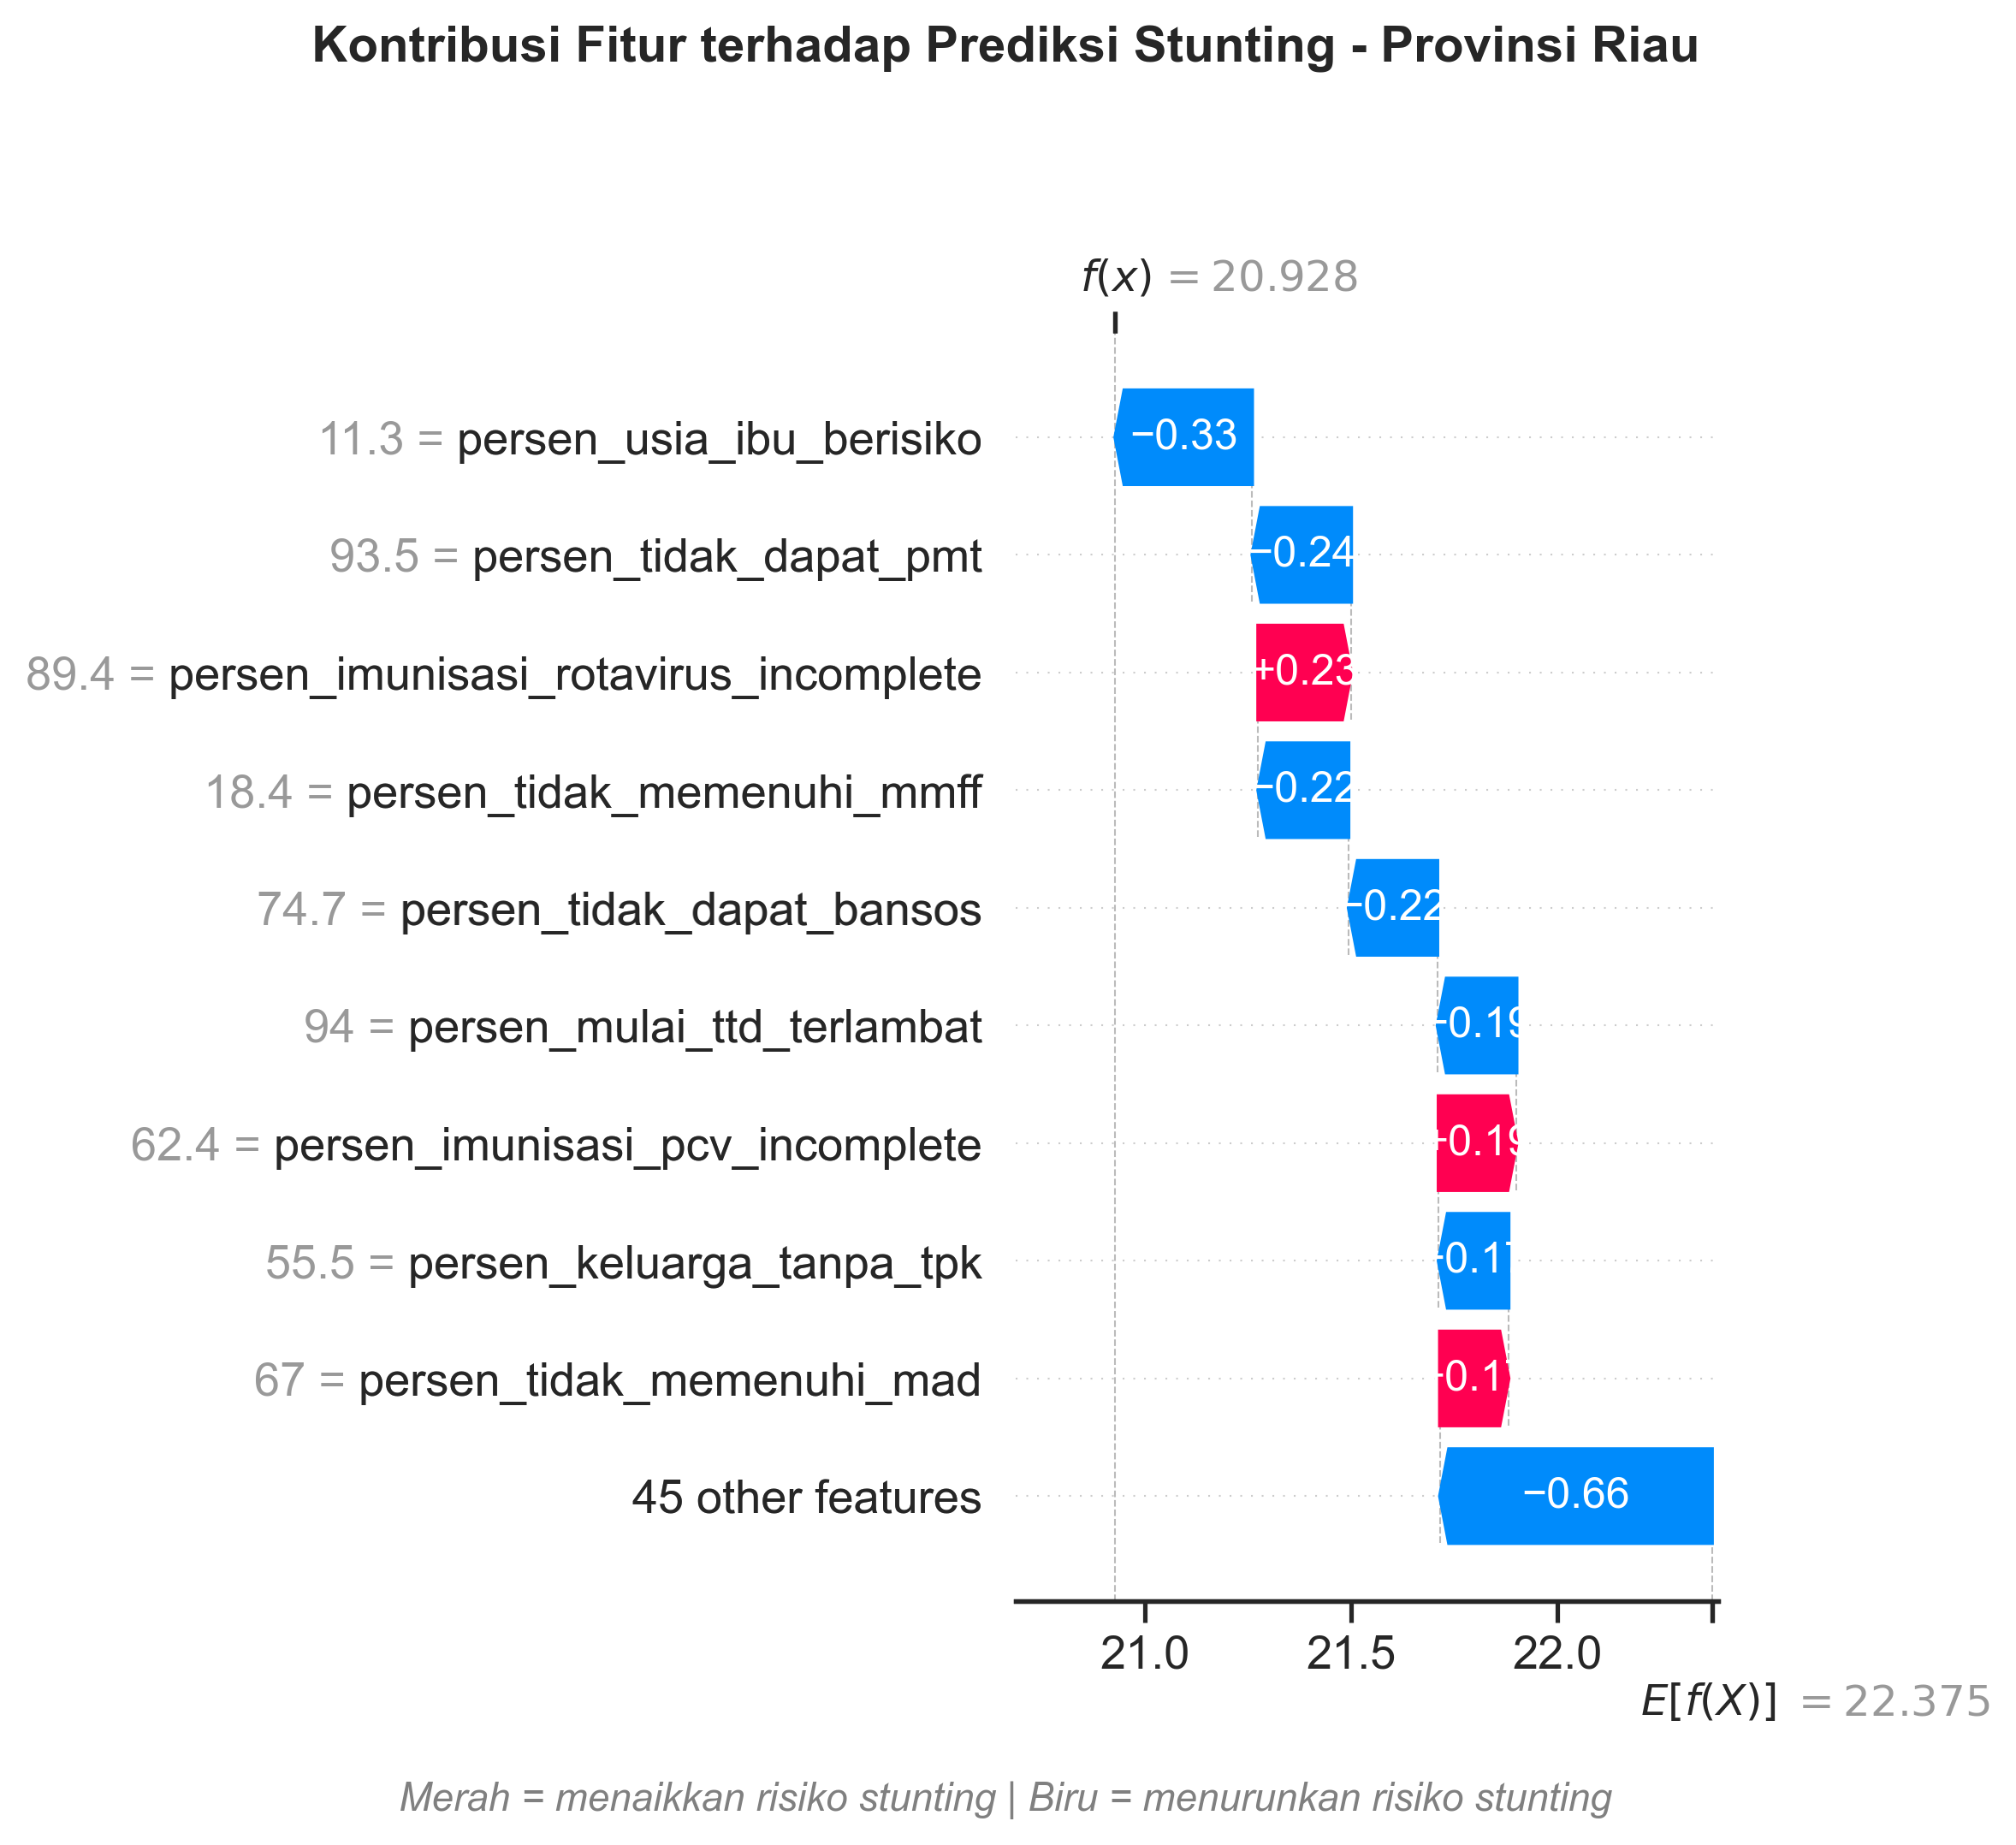
\includegraphics[width=0.48\textwidth]{figure/hasil_waterfall_stunting/waterfall_Riau.png} \\ \vspace{0.5cm}
    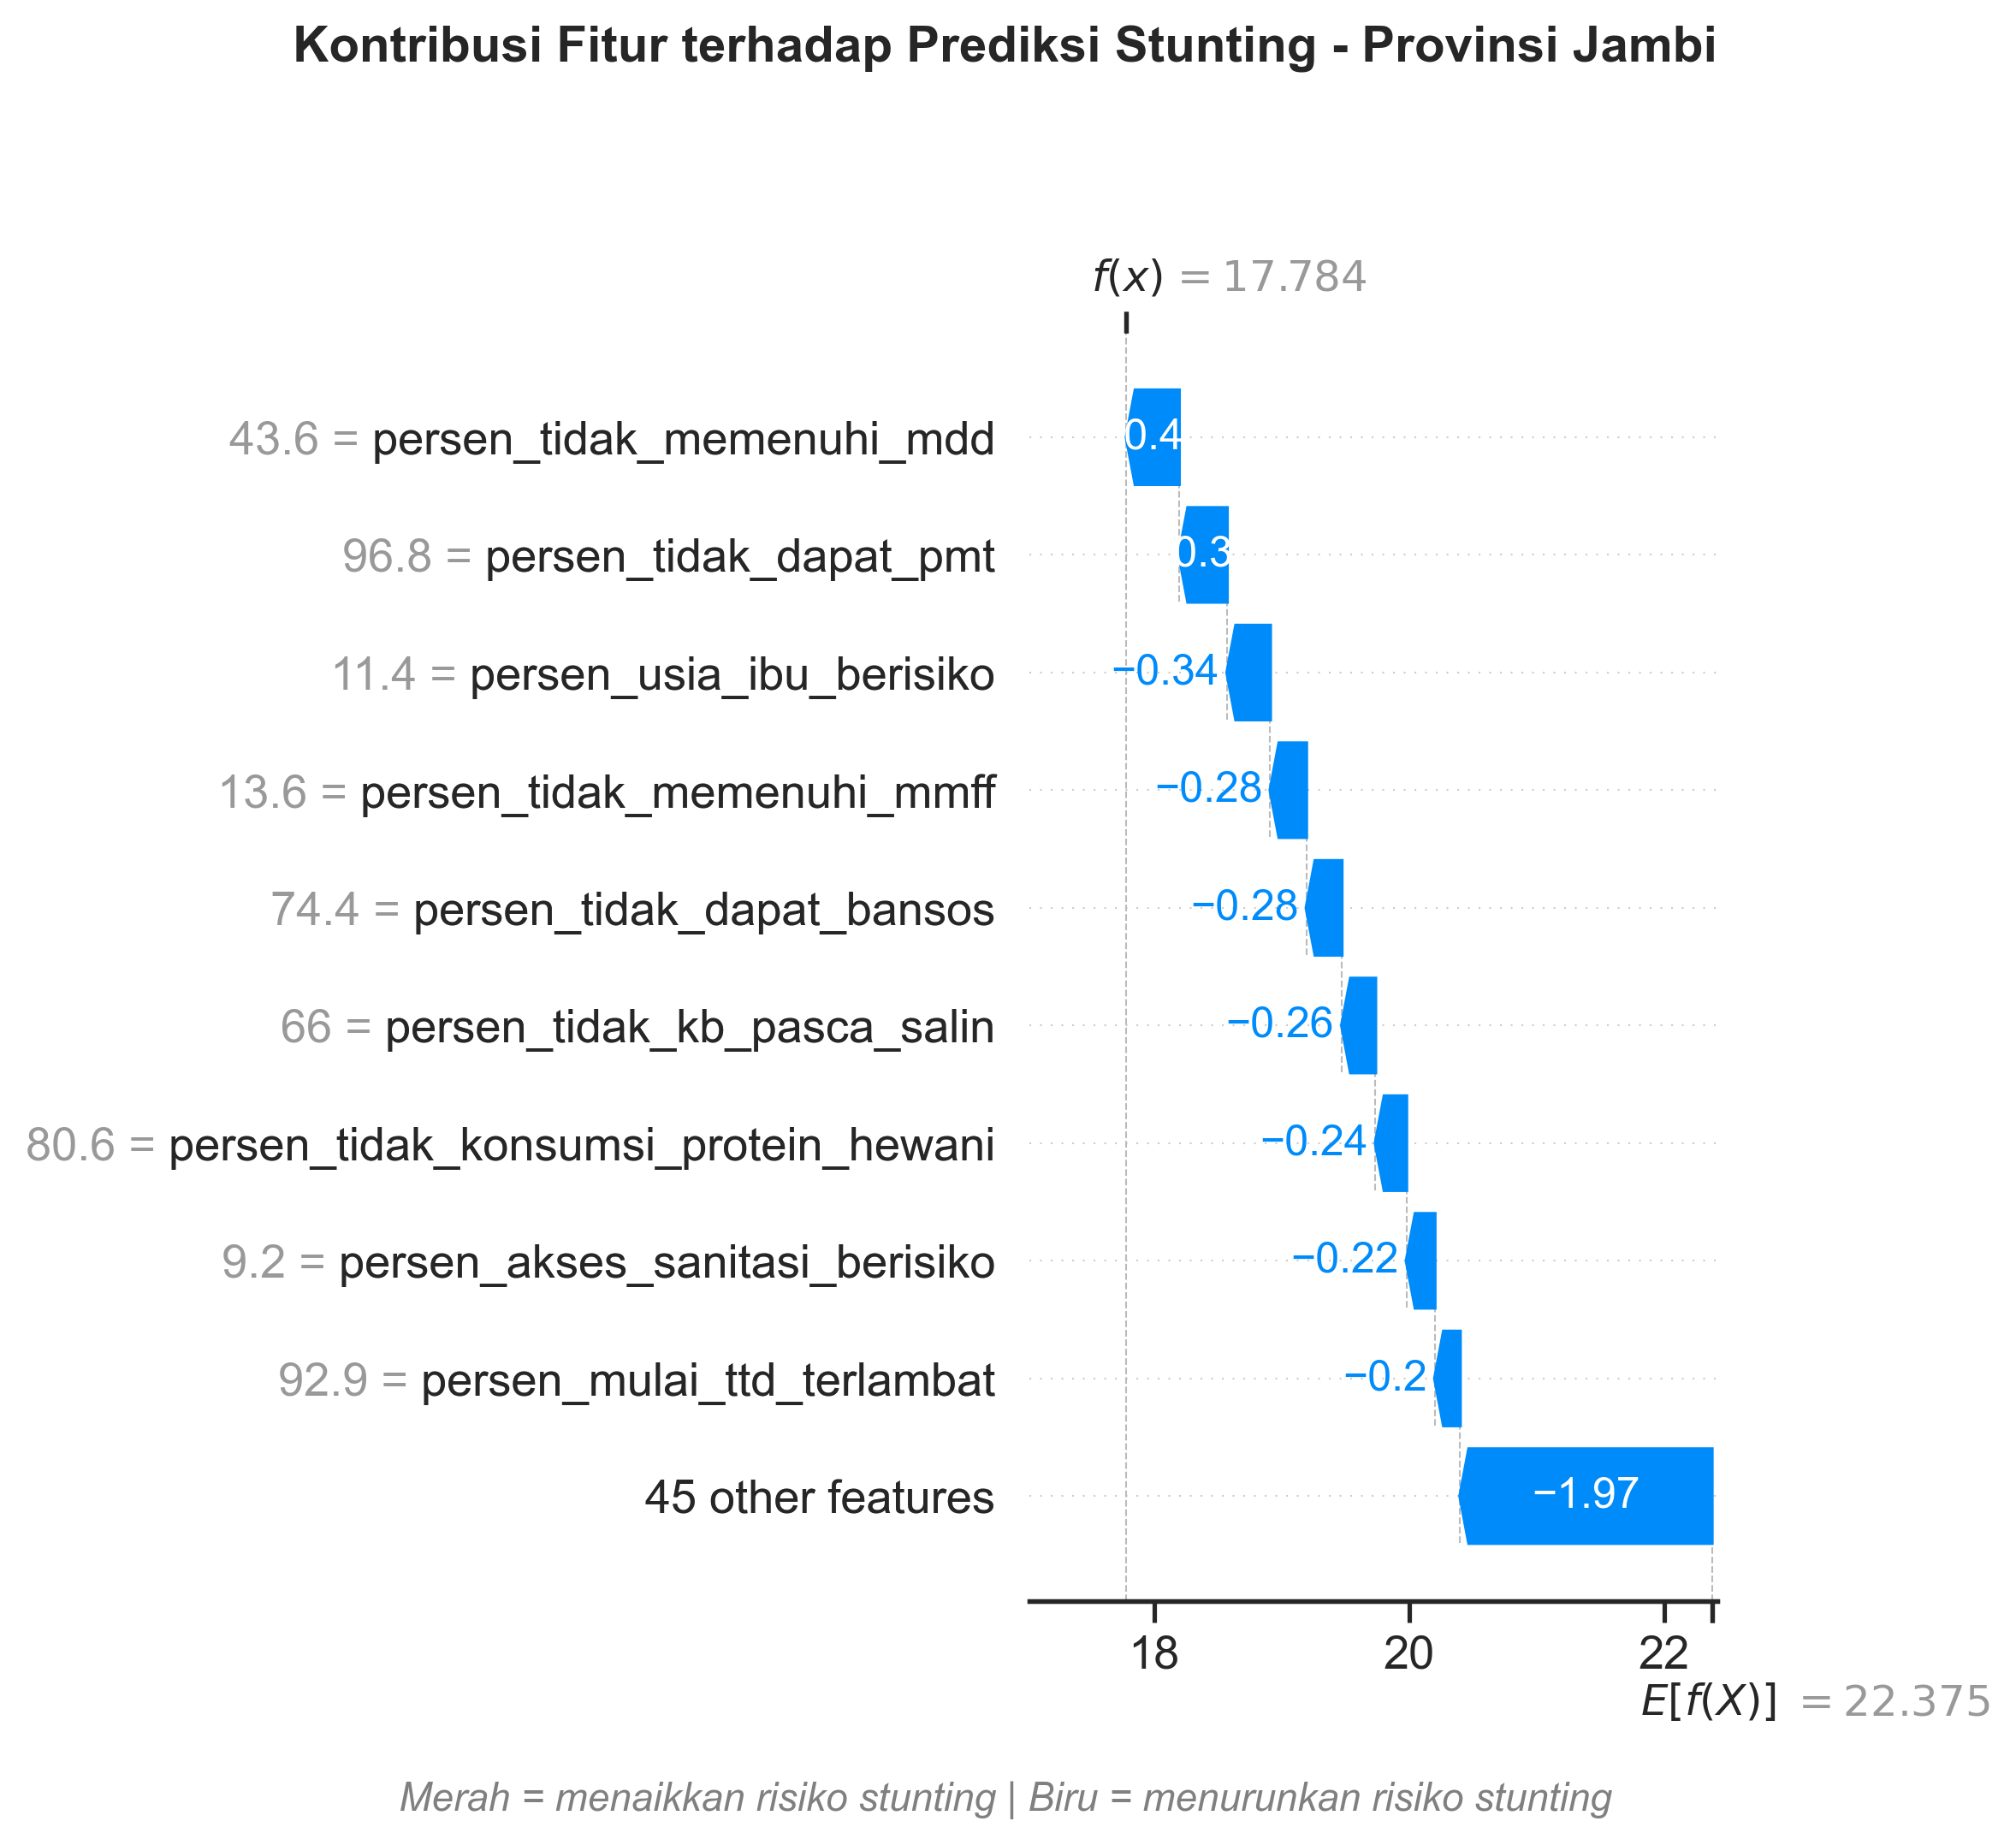
\includegraphics[width=0.48\textwidth]{figure/hasil_waterfall_stunting/waterfall_Jambi.png} \hfill
    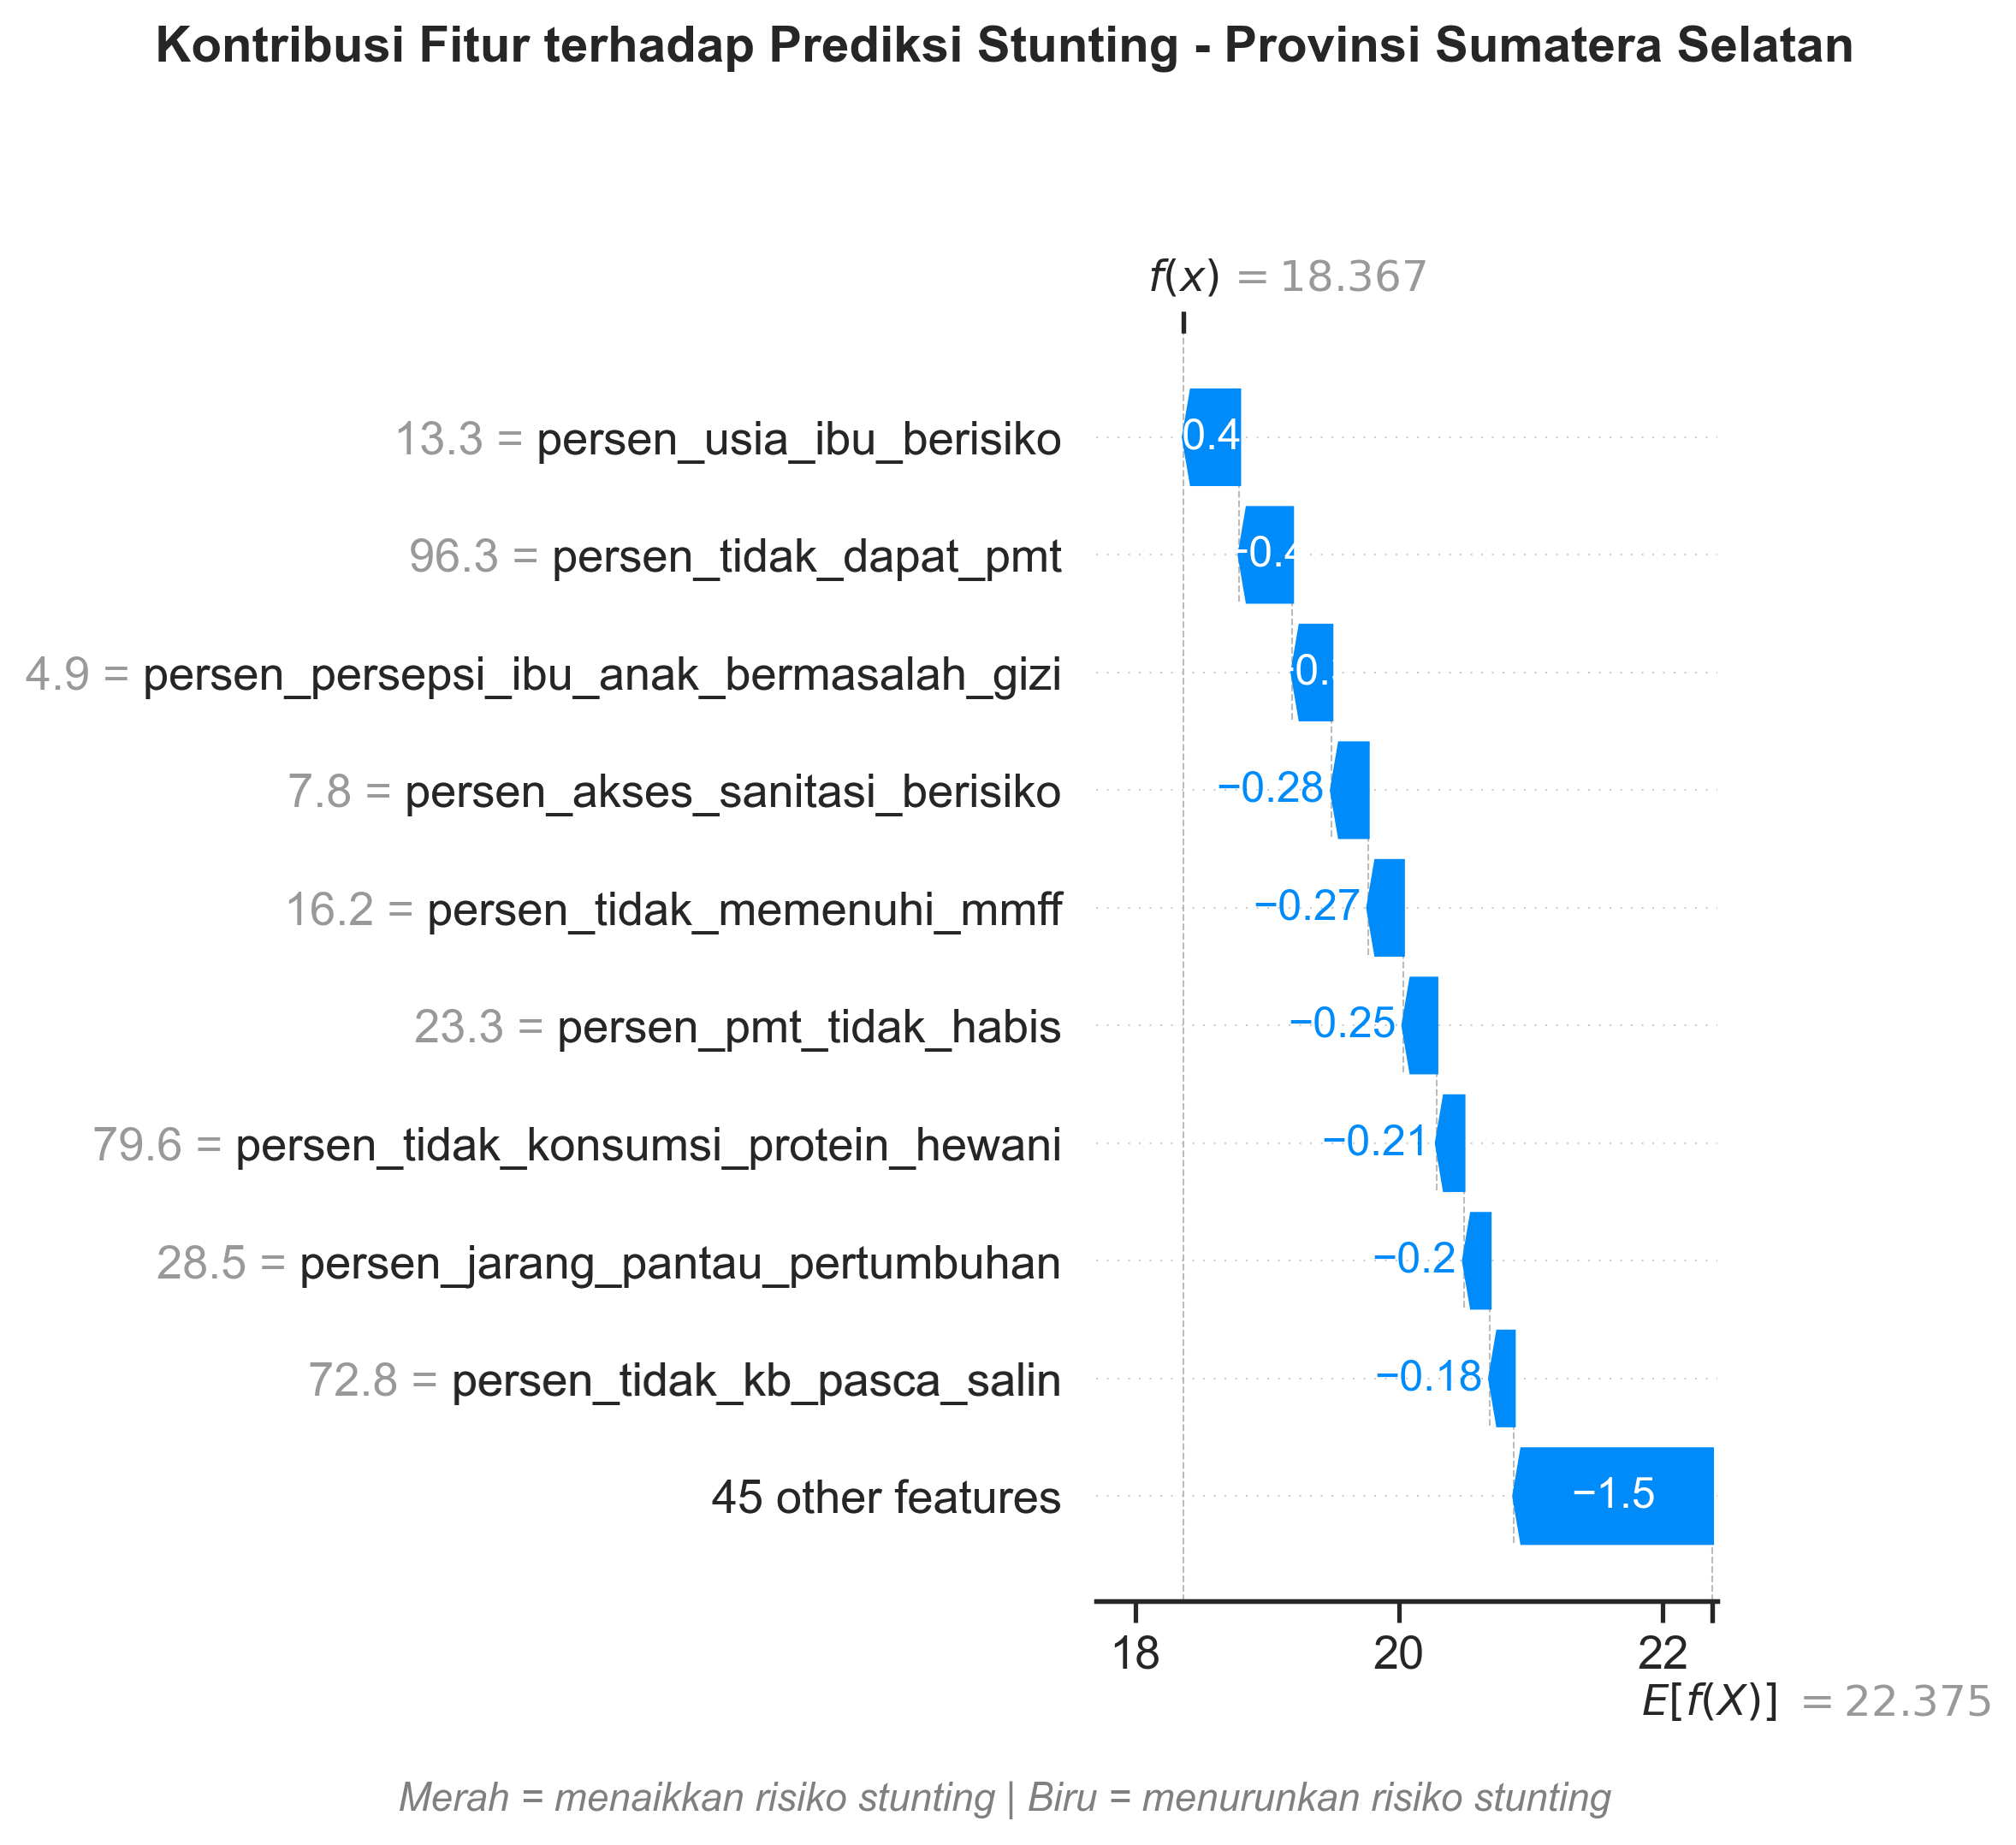
\includegraphics[width=0.48\textwidth]{figure/hasil_waterfall_stunting/waterfall_Sumatera_Selatan.png}
\end{center}

\newpage
\begin{figure}[H]
    \centering
    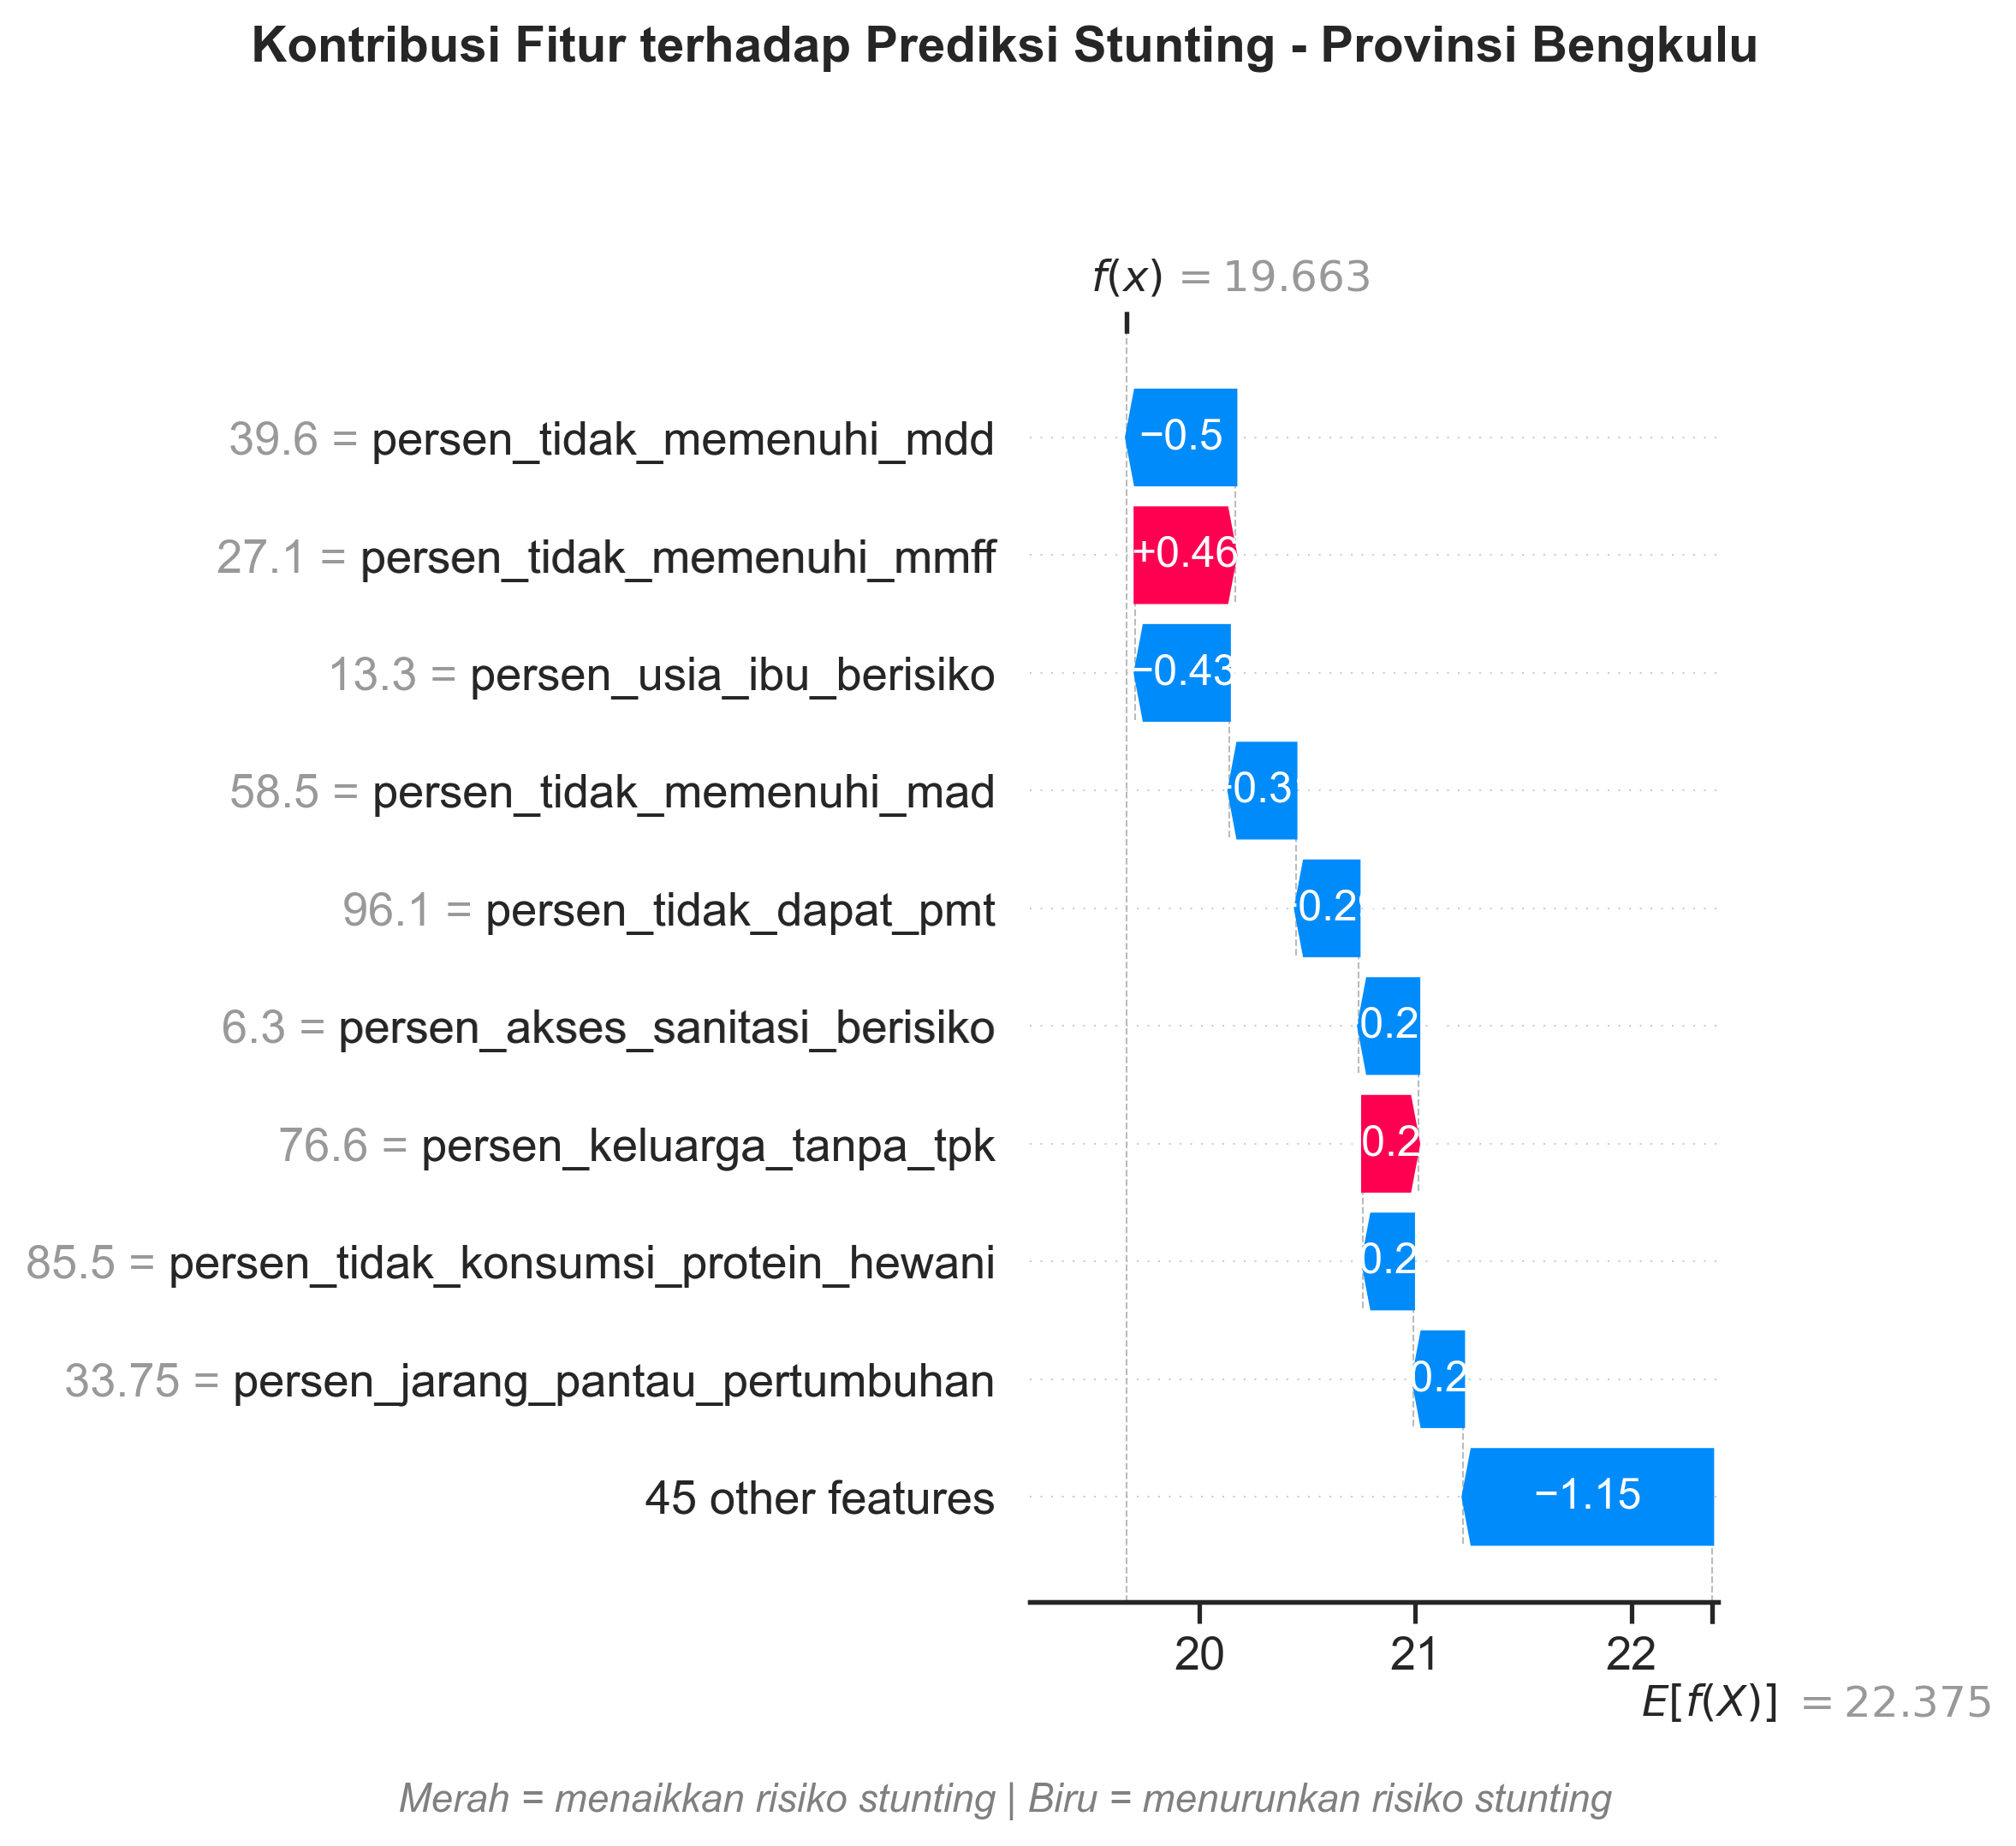
\includegraphics[width=0.48\textwidth]{figure/hasil_waterfall_stunting/waterfall_Bengkulu.png} \hfill
    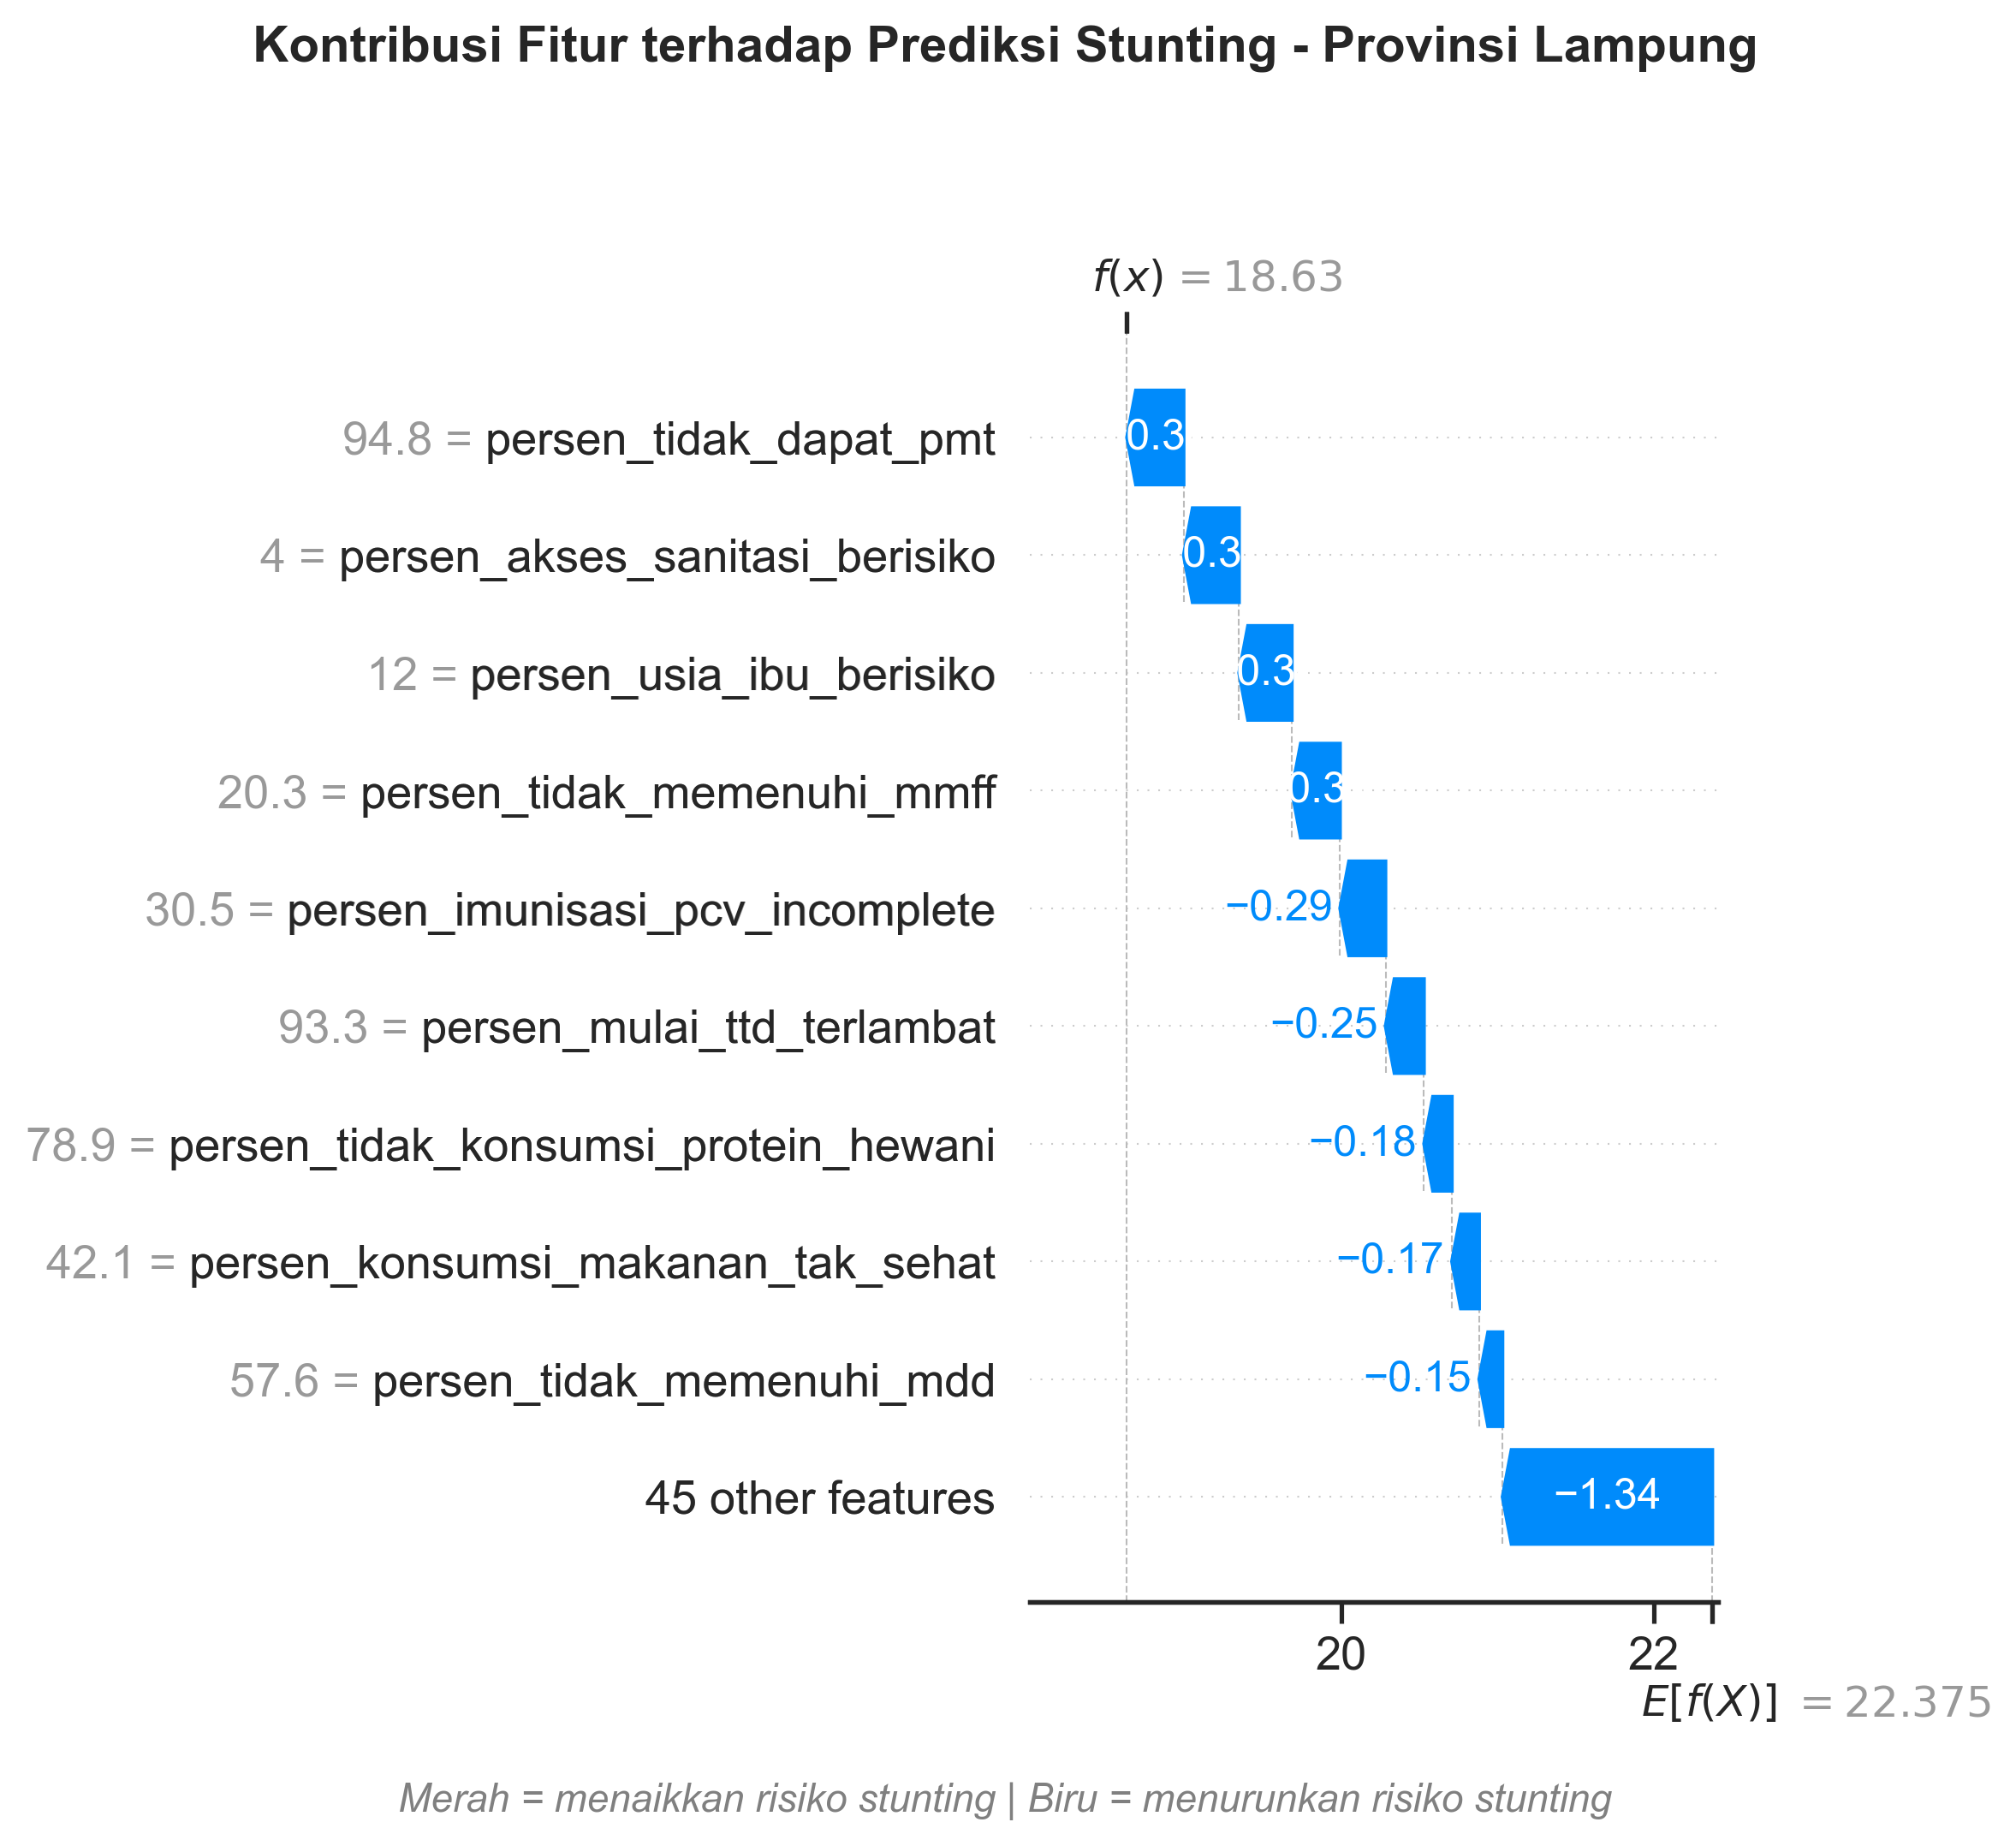
\includegraphics[width=0.48\textwidth]{figure/hasil_waterfall_stunting/waterfall_Lampung.png} \\ \vspace{0.5cm}
    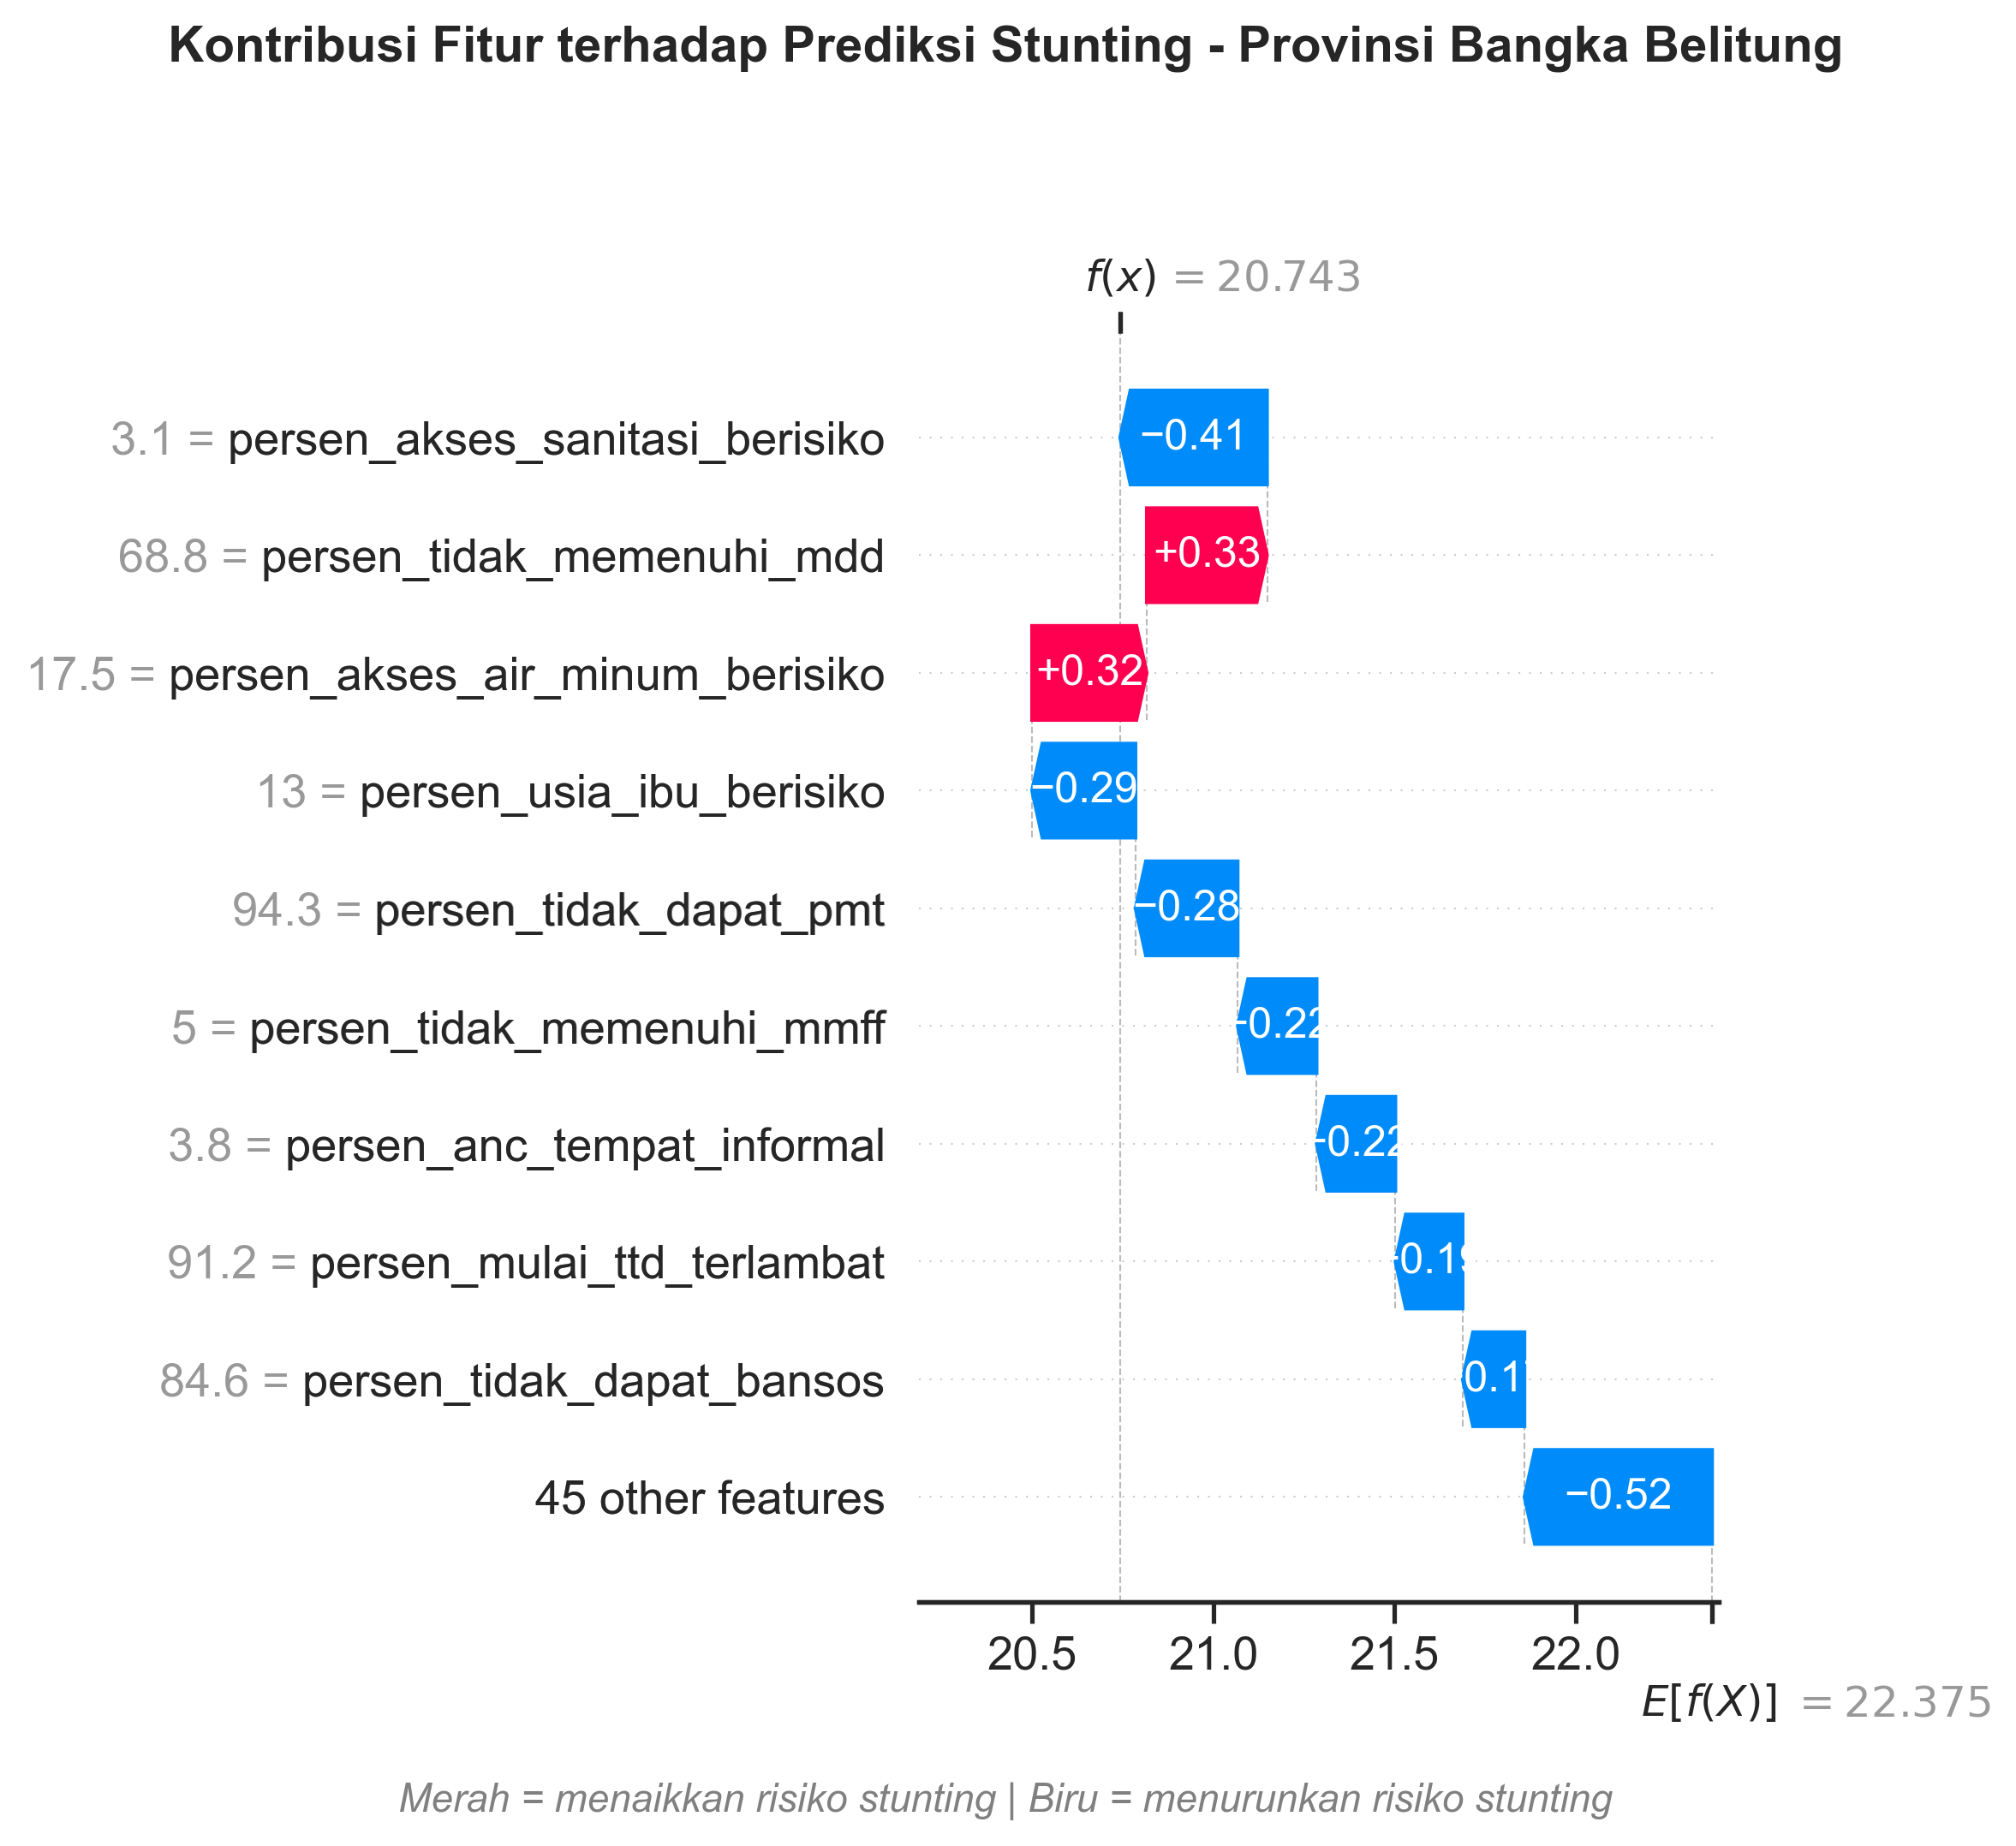
\includegraphics[width=0.48\textwidth]{figure/hasil_waterfall_stunting/waterfall_Bangka_Belitung.png} \hfill
    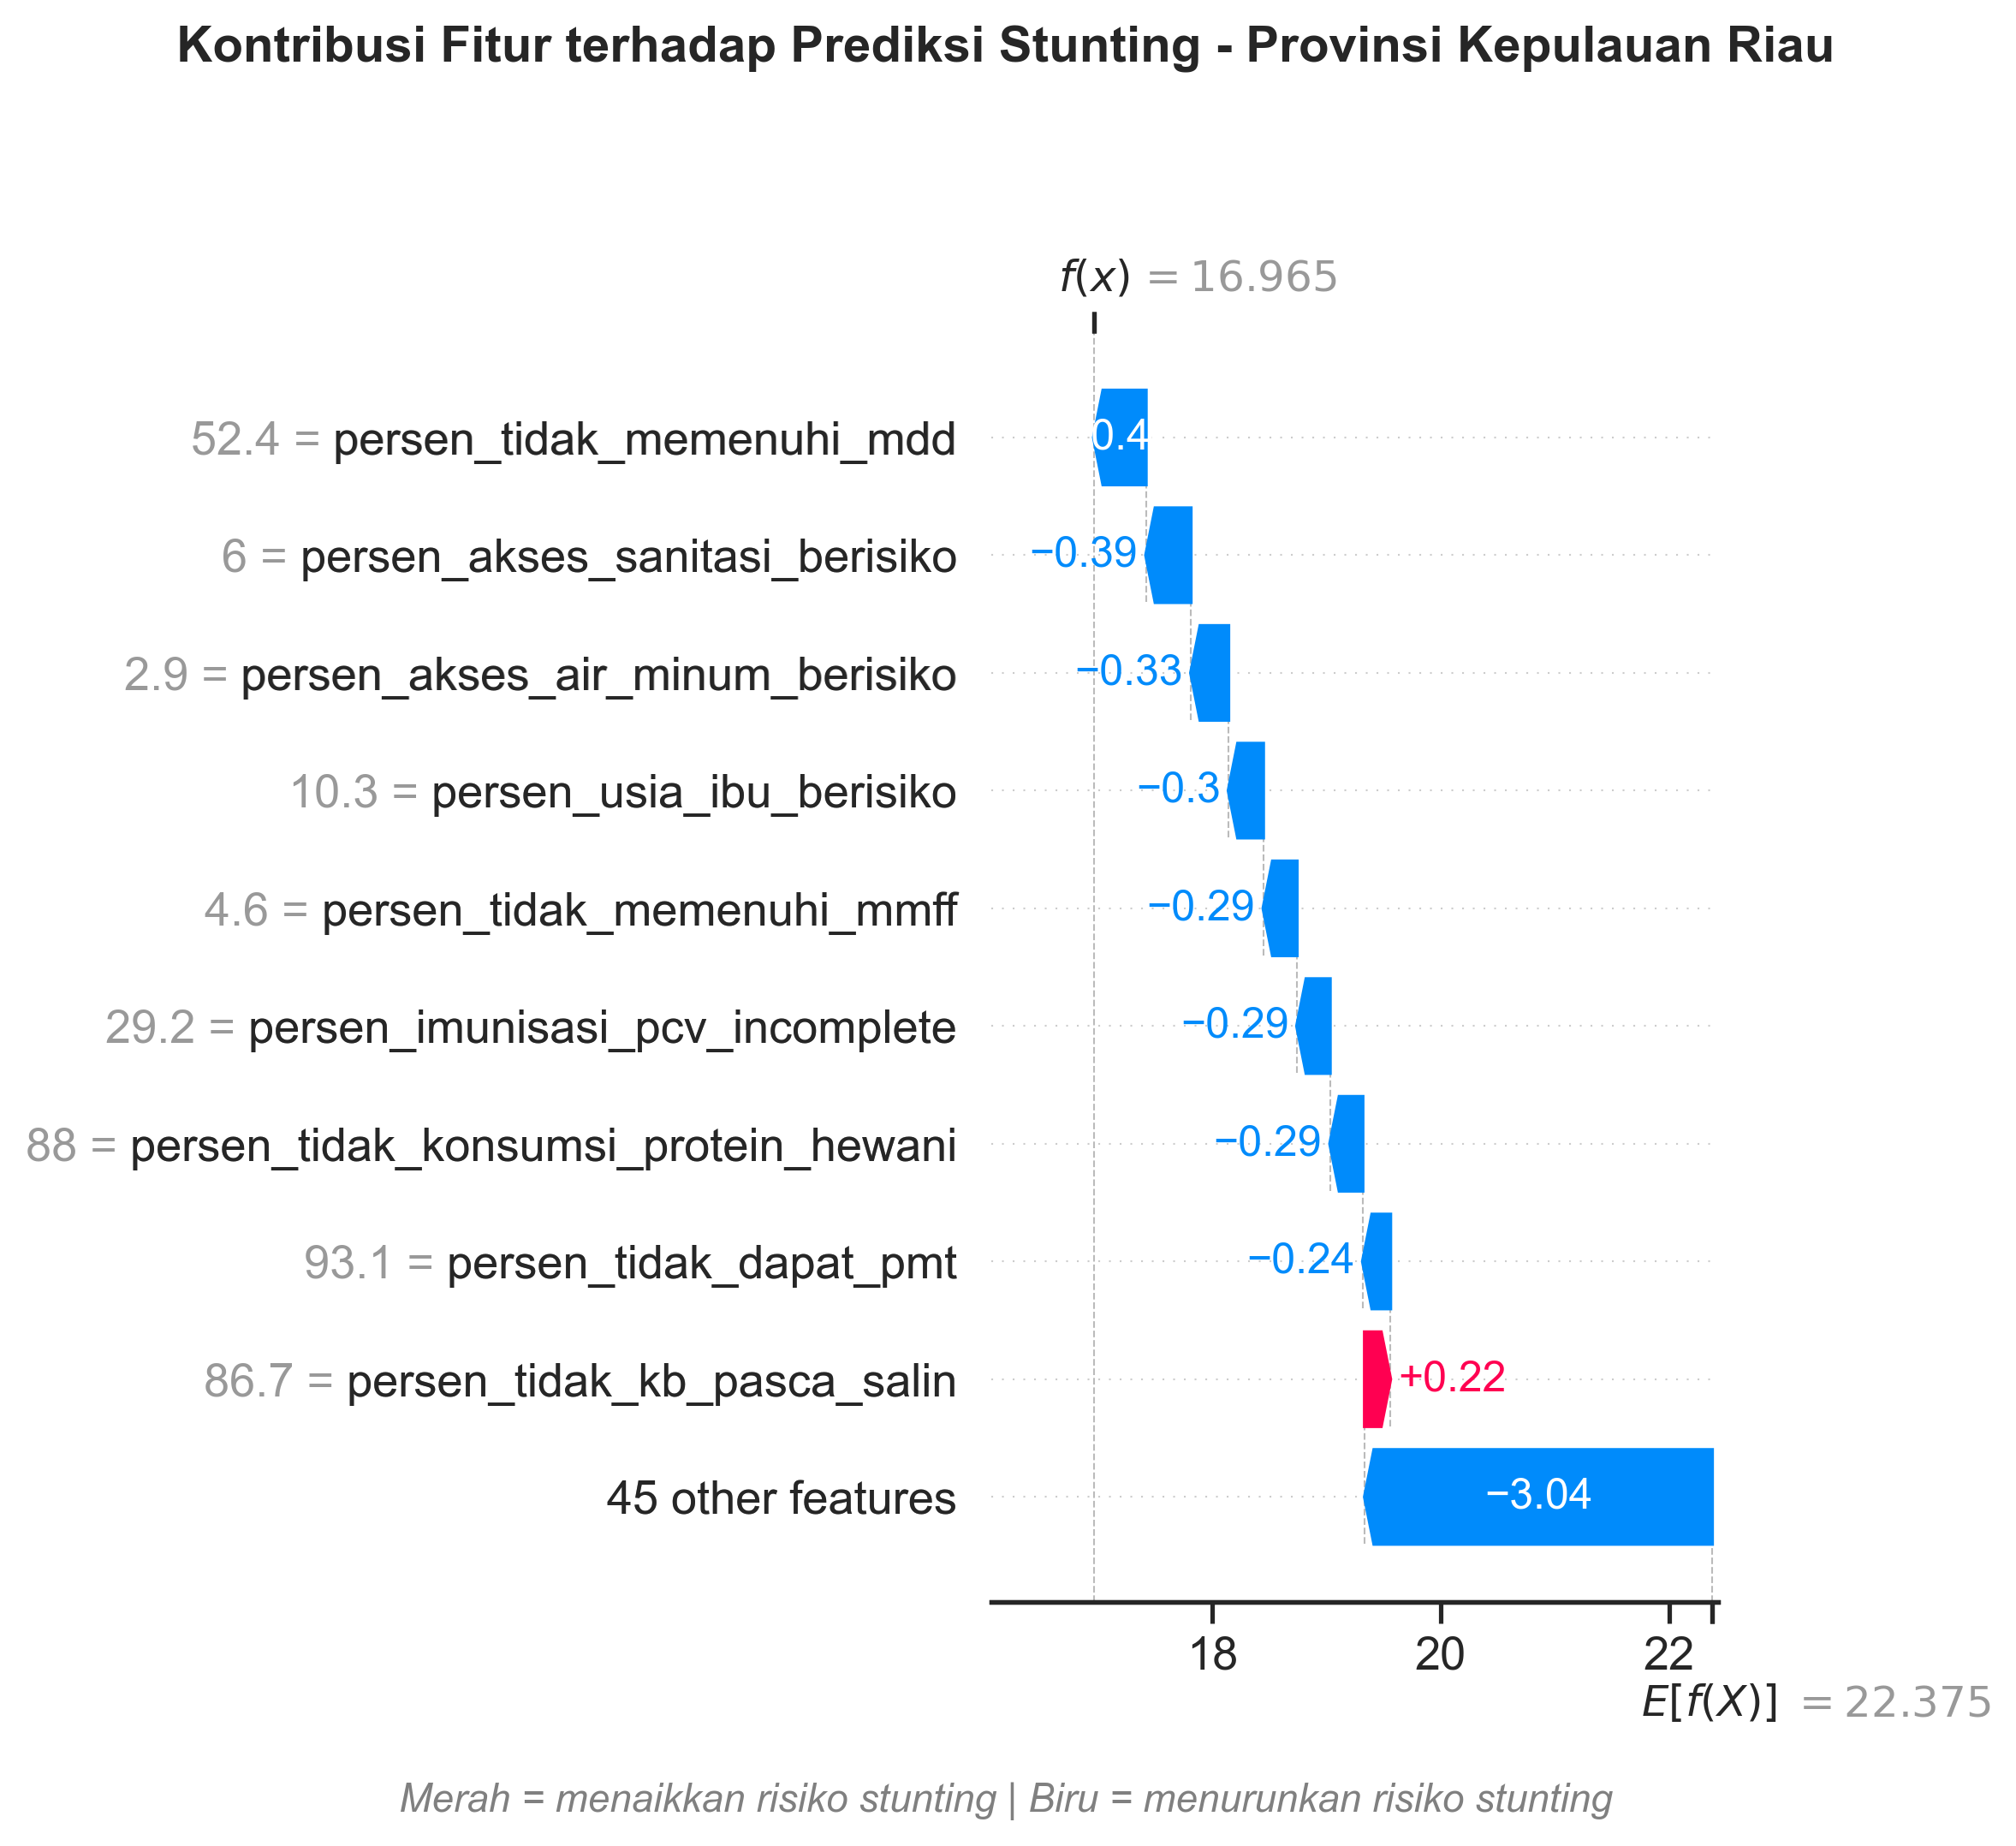
\includegraphics[width=0.48\textwidth]{figure/hasil_waterfall_stunting/waterfall_Kepulauan_Riau.png} \\ \vspace{0.5cm}
    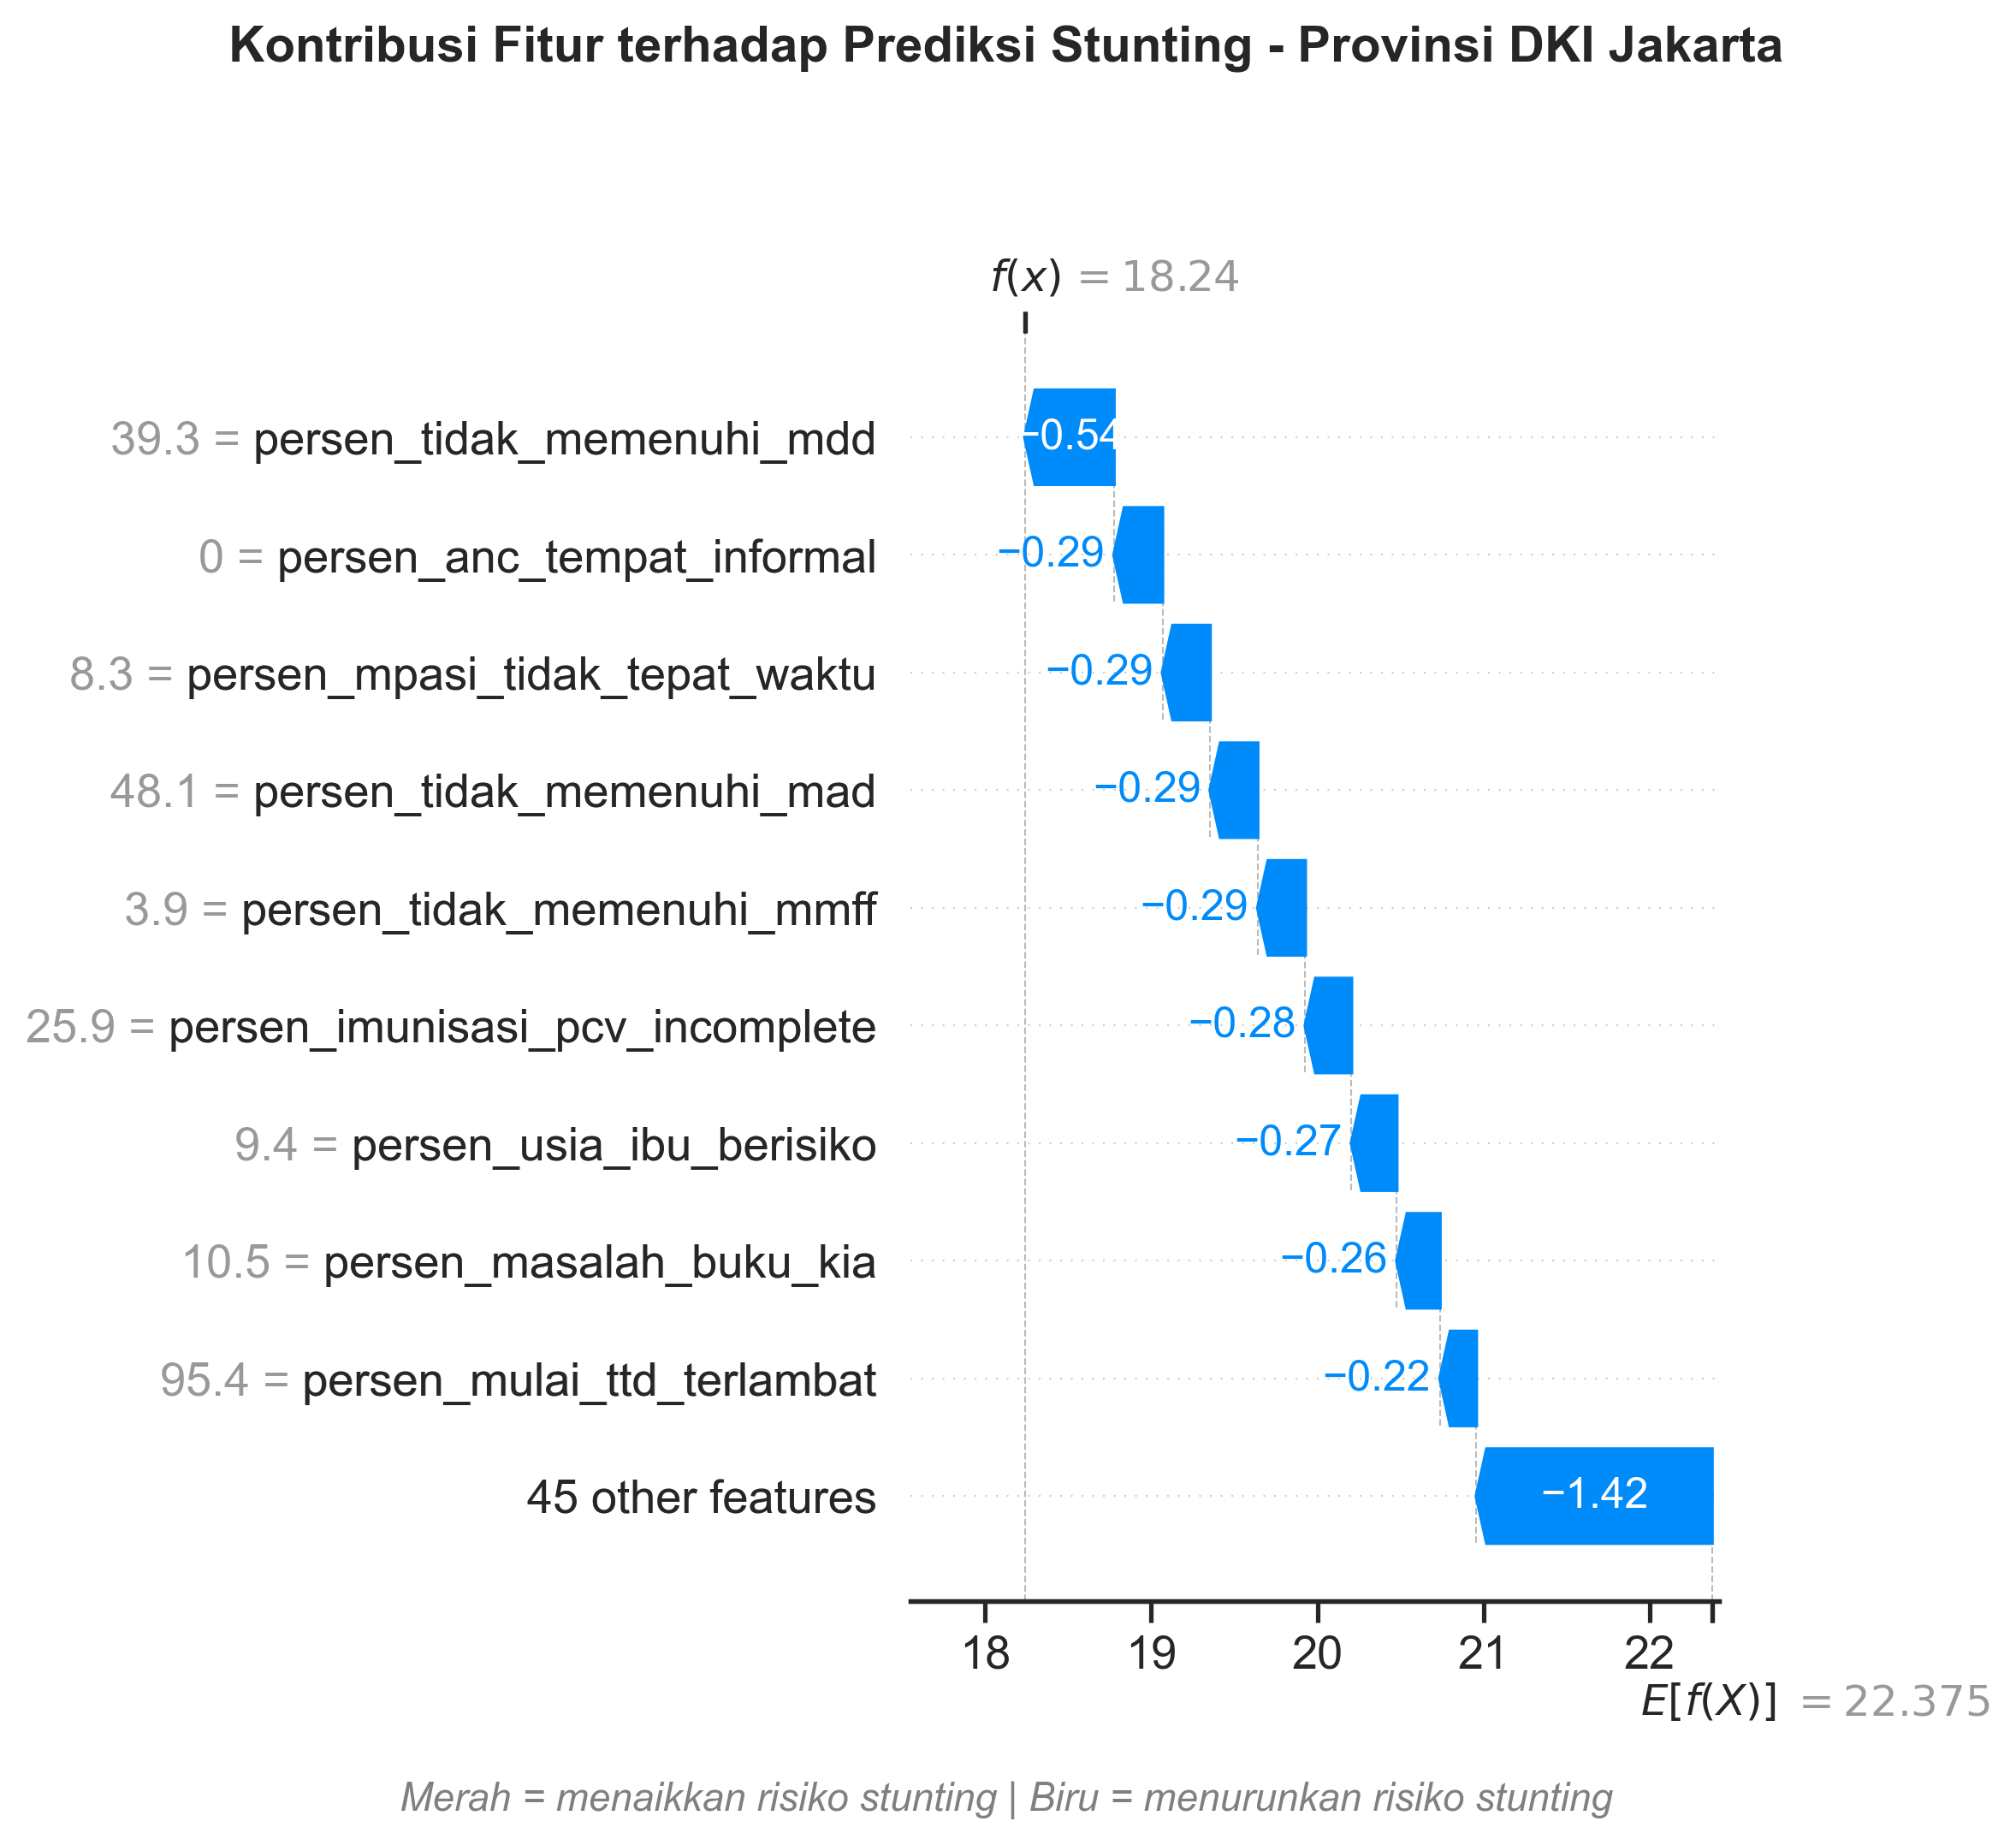
\includegraphics[width=0.48\textwidth]{figure/hasil_waterfall_stunting/waterfall_DKI_Jakarta.png} \hfill
    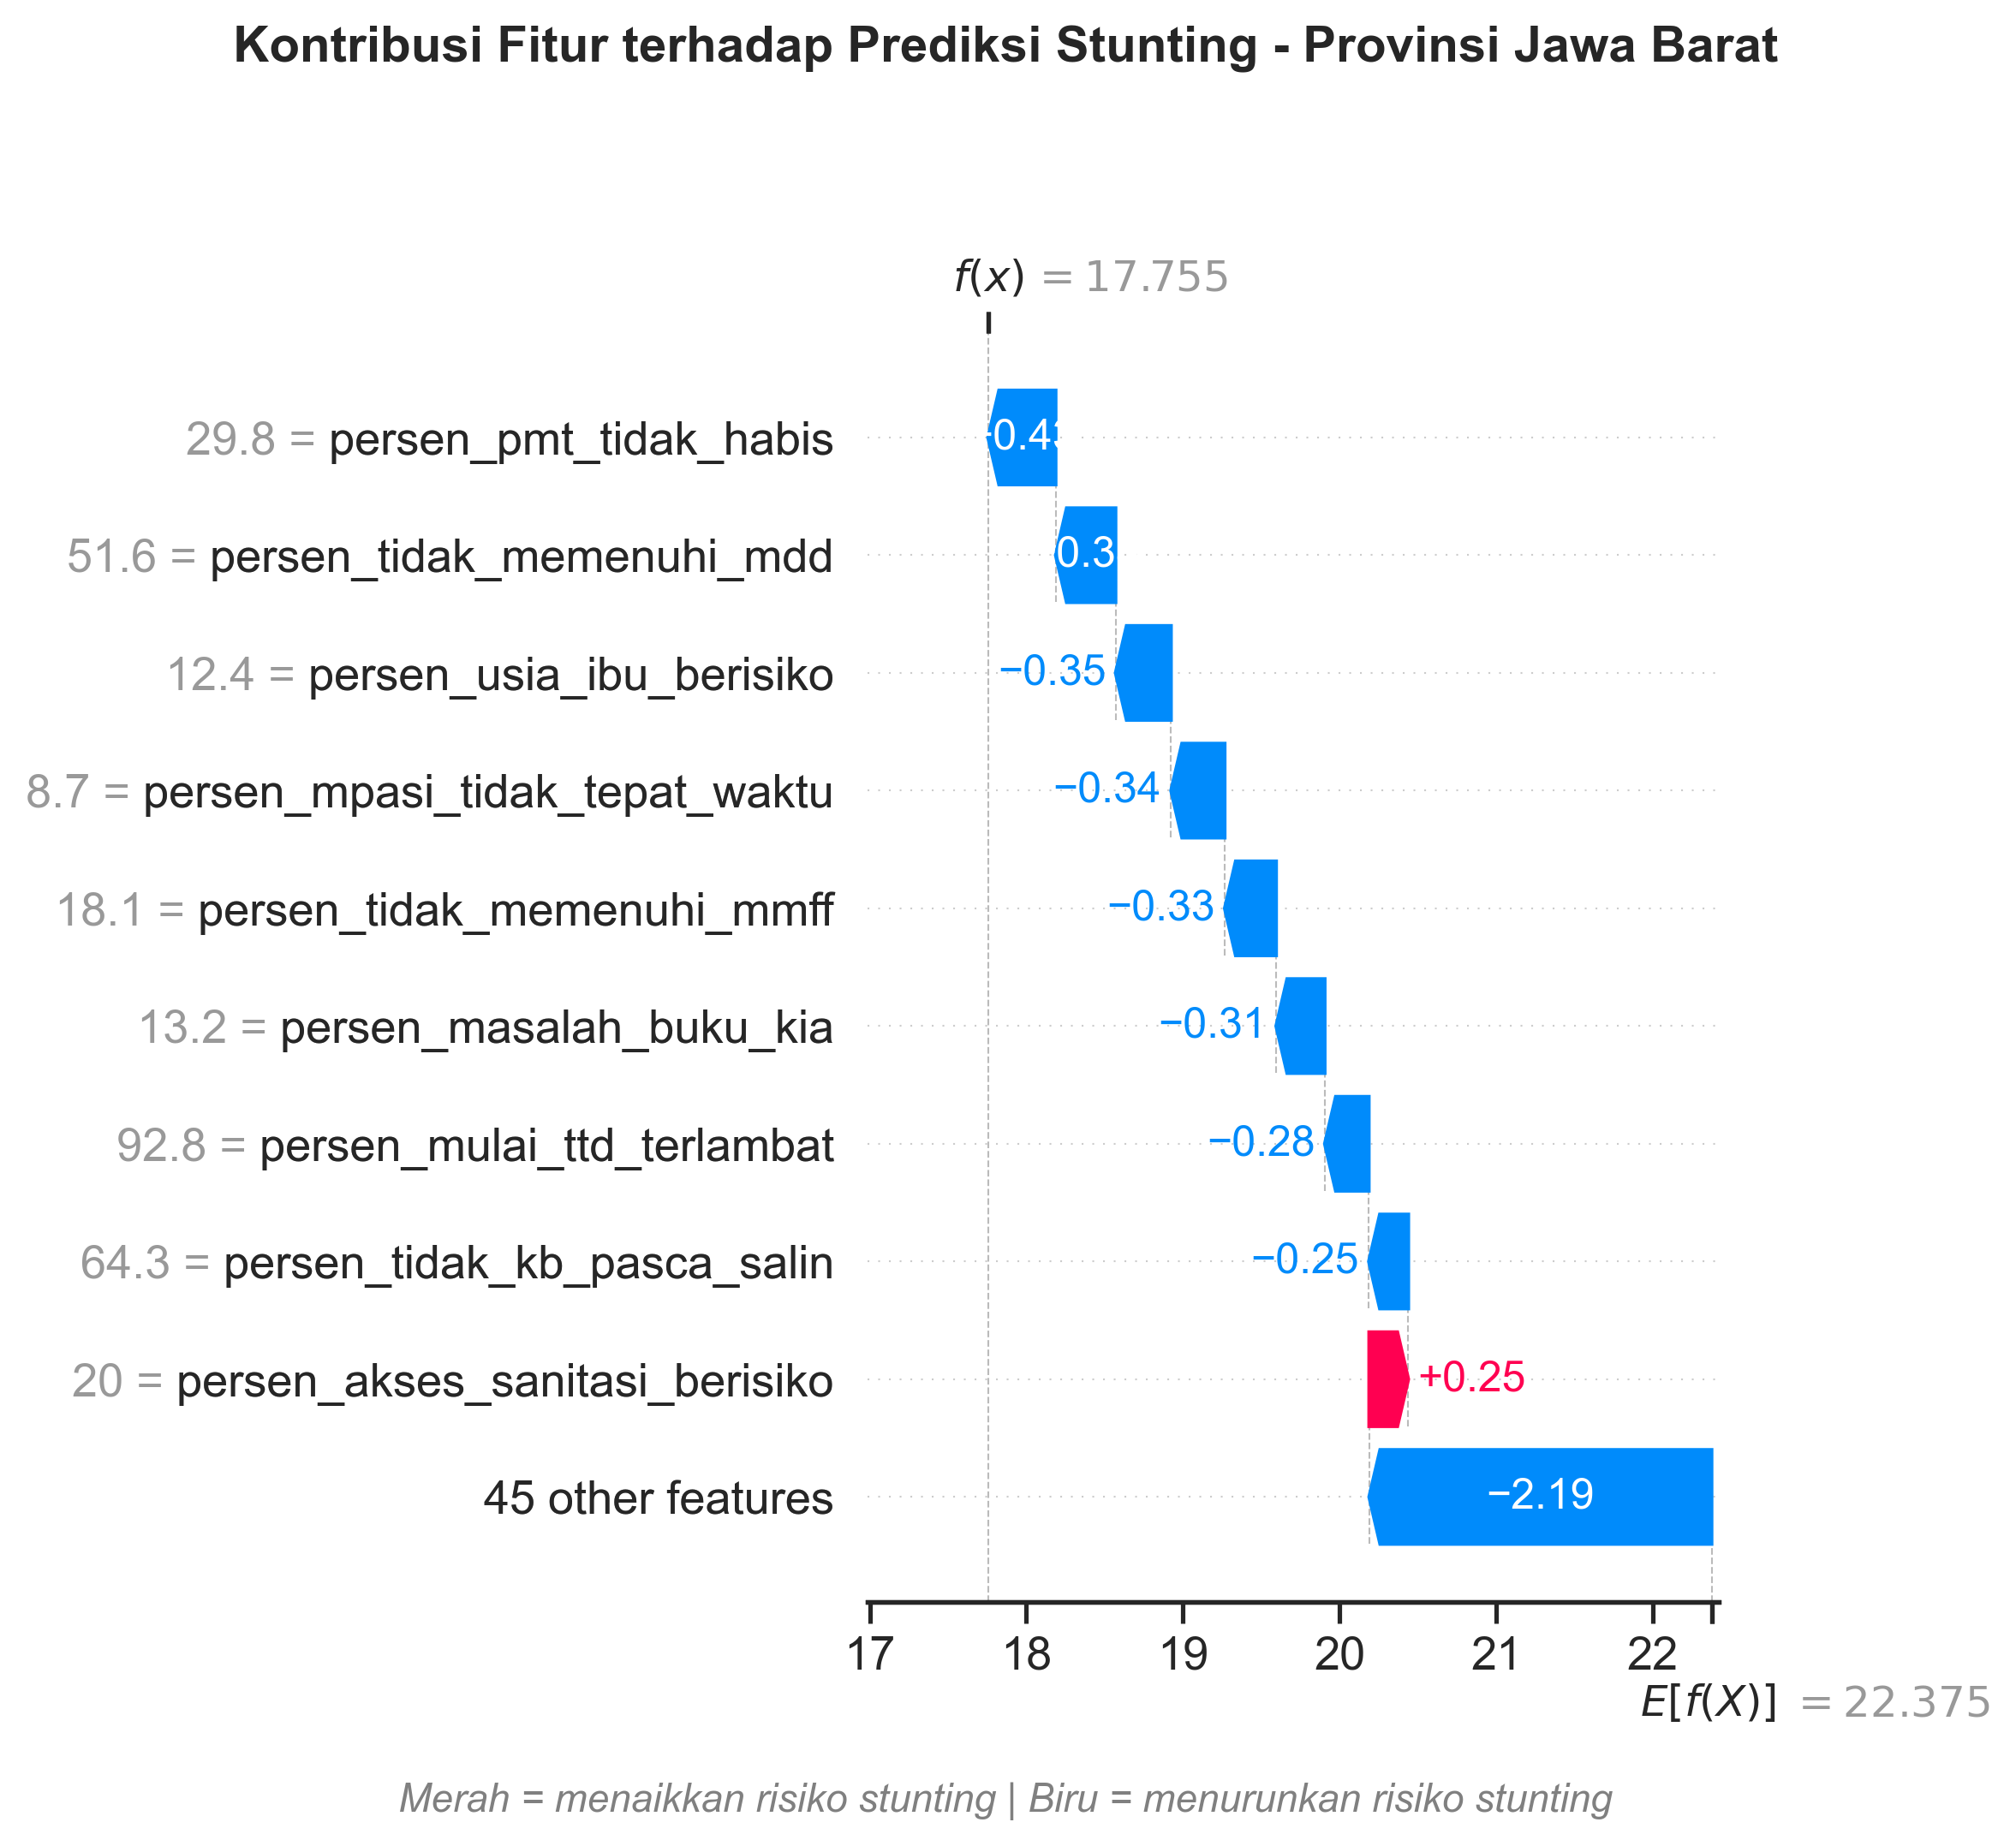
\includegraphics[width=0.48\textwidth]{figure/hasil_waterfall_stunting/waterfall_Jawa_Barat.png}
\end{figure}

\newpage
\begin{figure}[H]
    \centering
    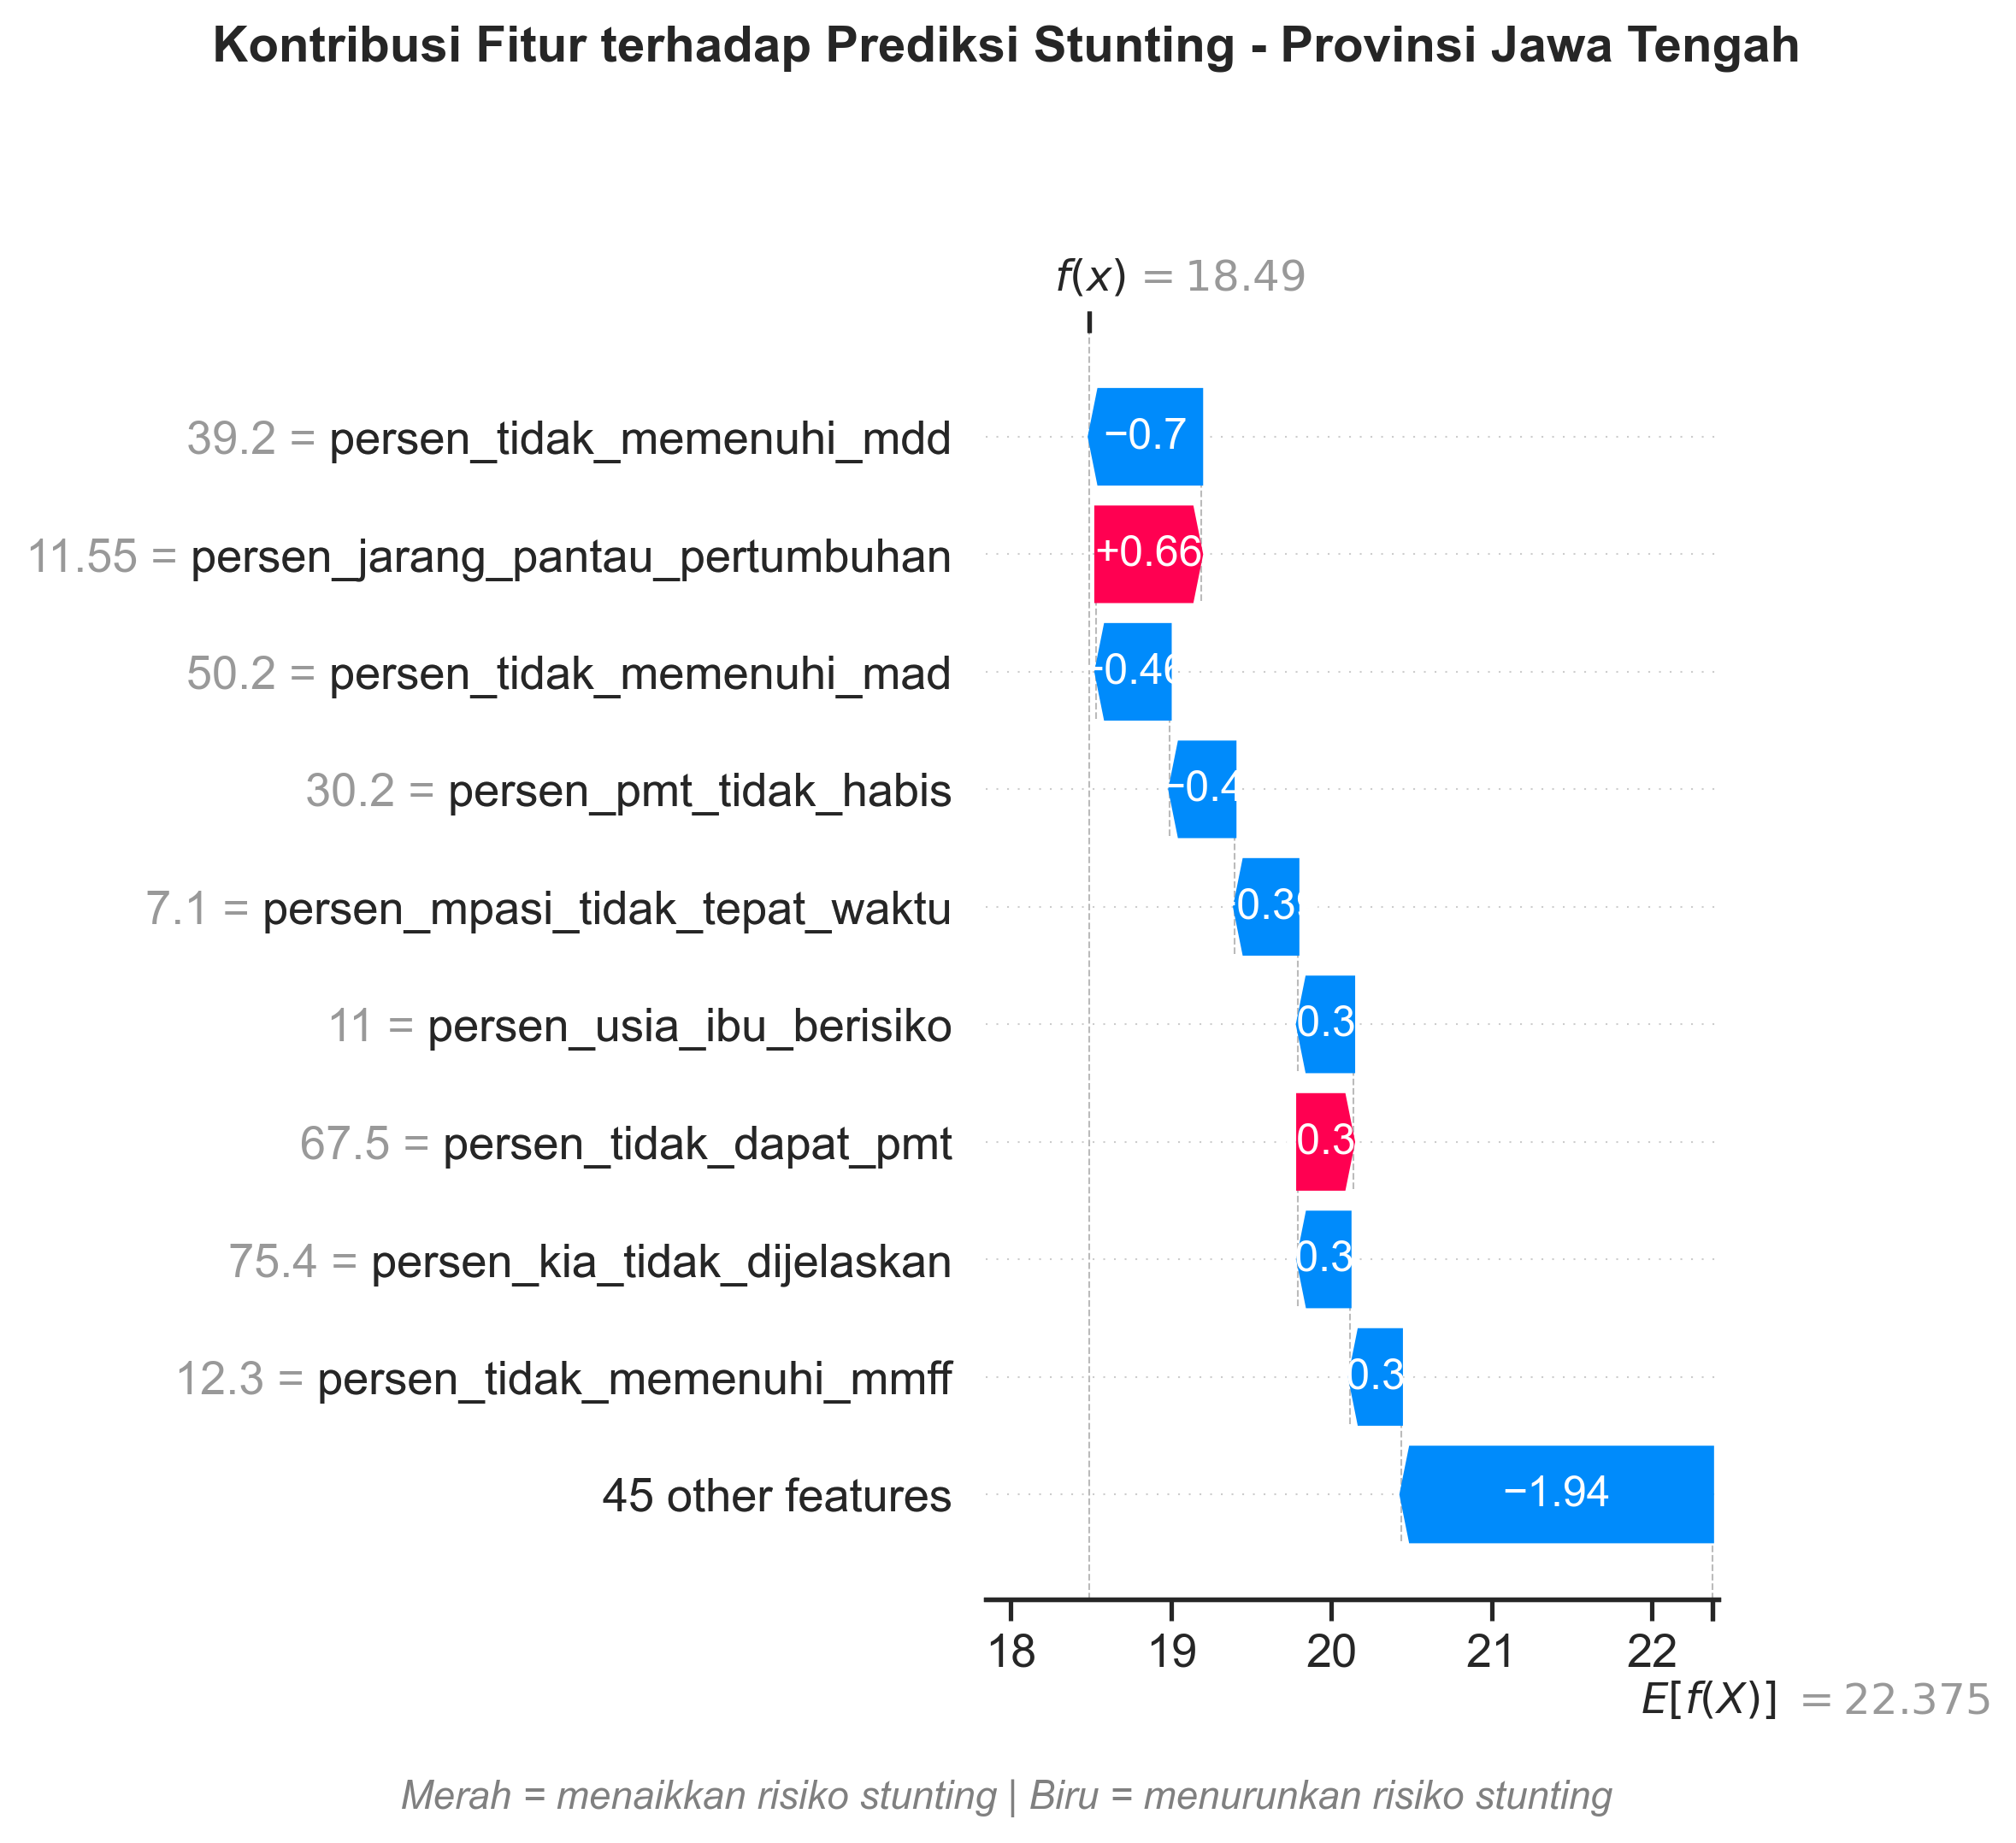
\includegraphics[width=0.48\textwidth]{figure/hasil_waterfall_stunting/waterfall_Jawa_Tengah.png} \hfill
    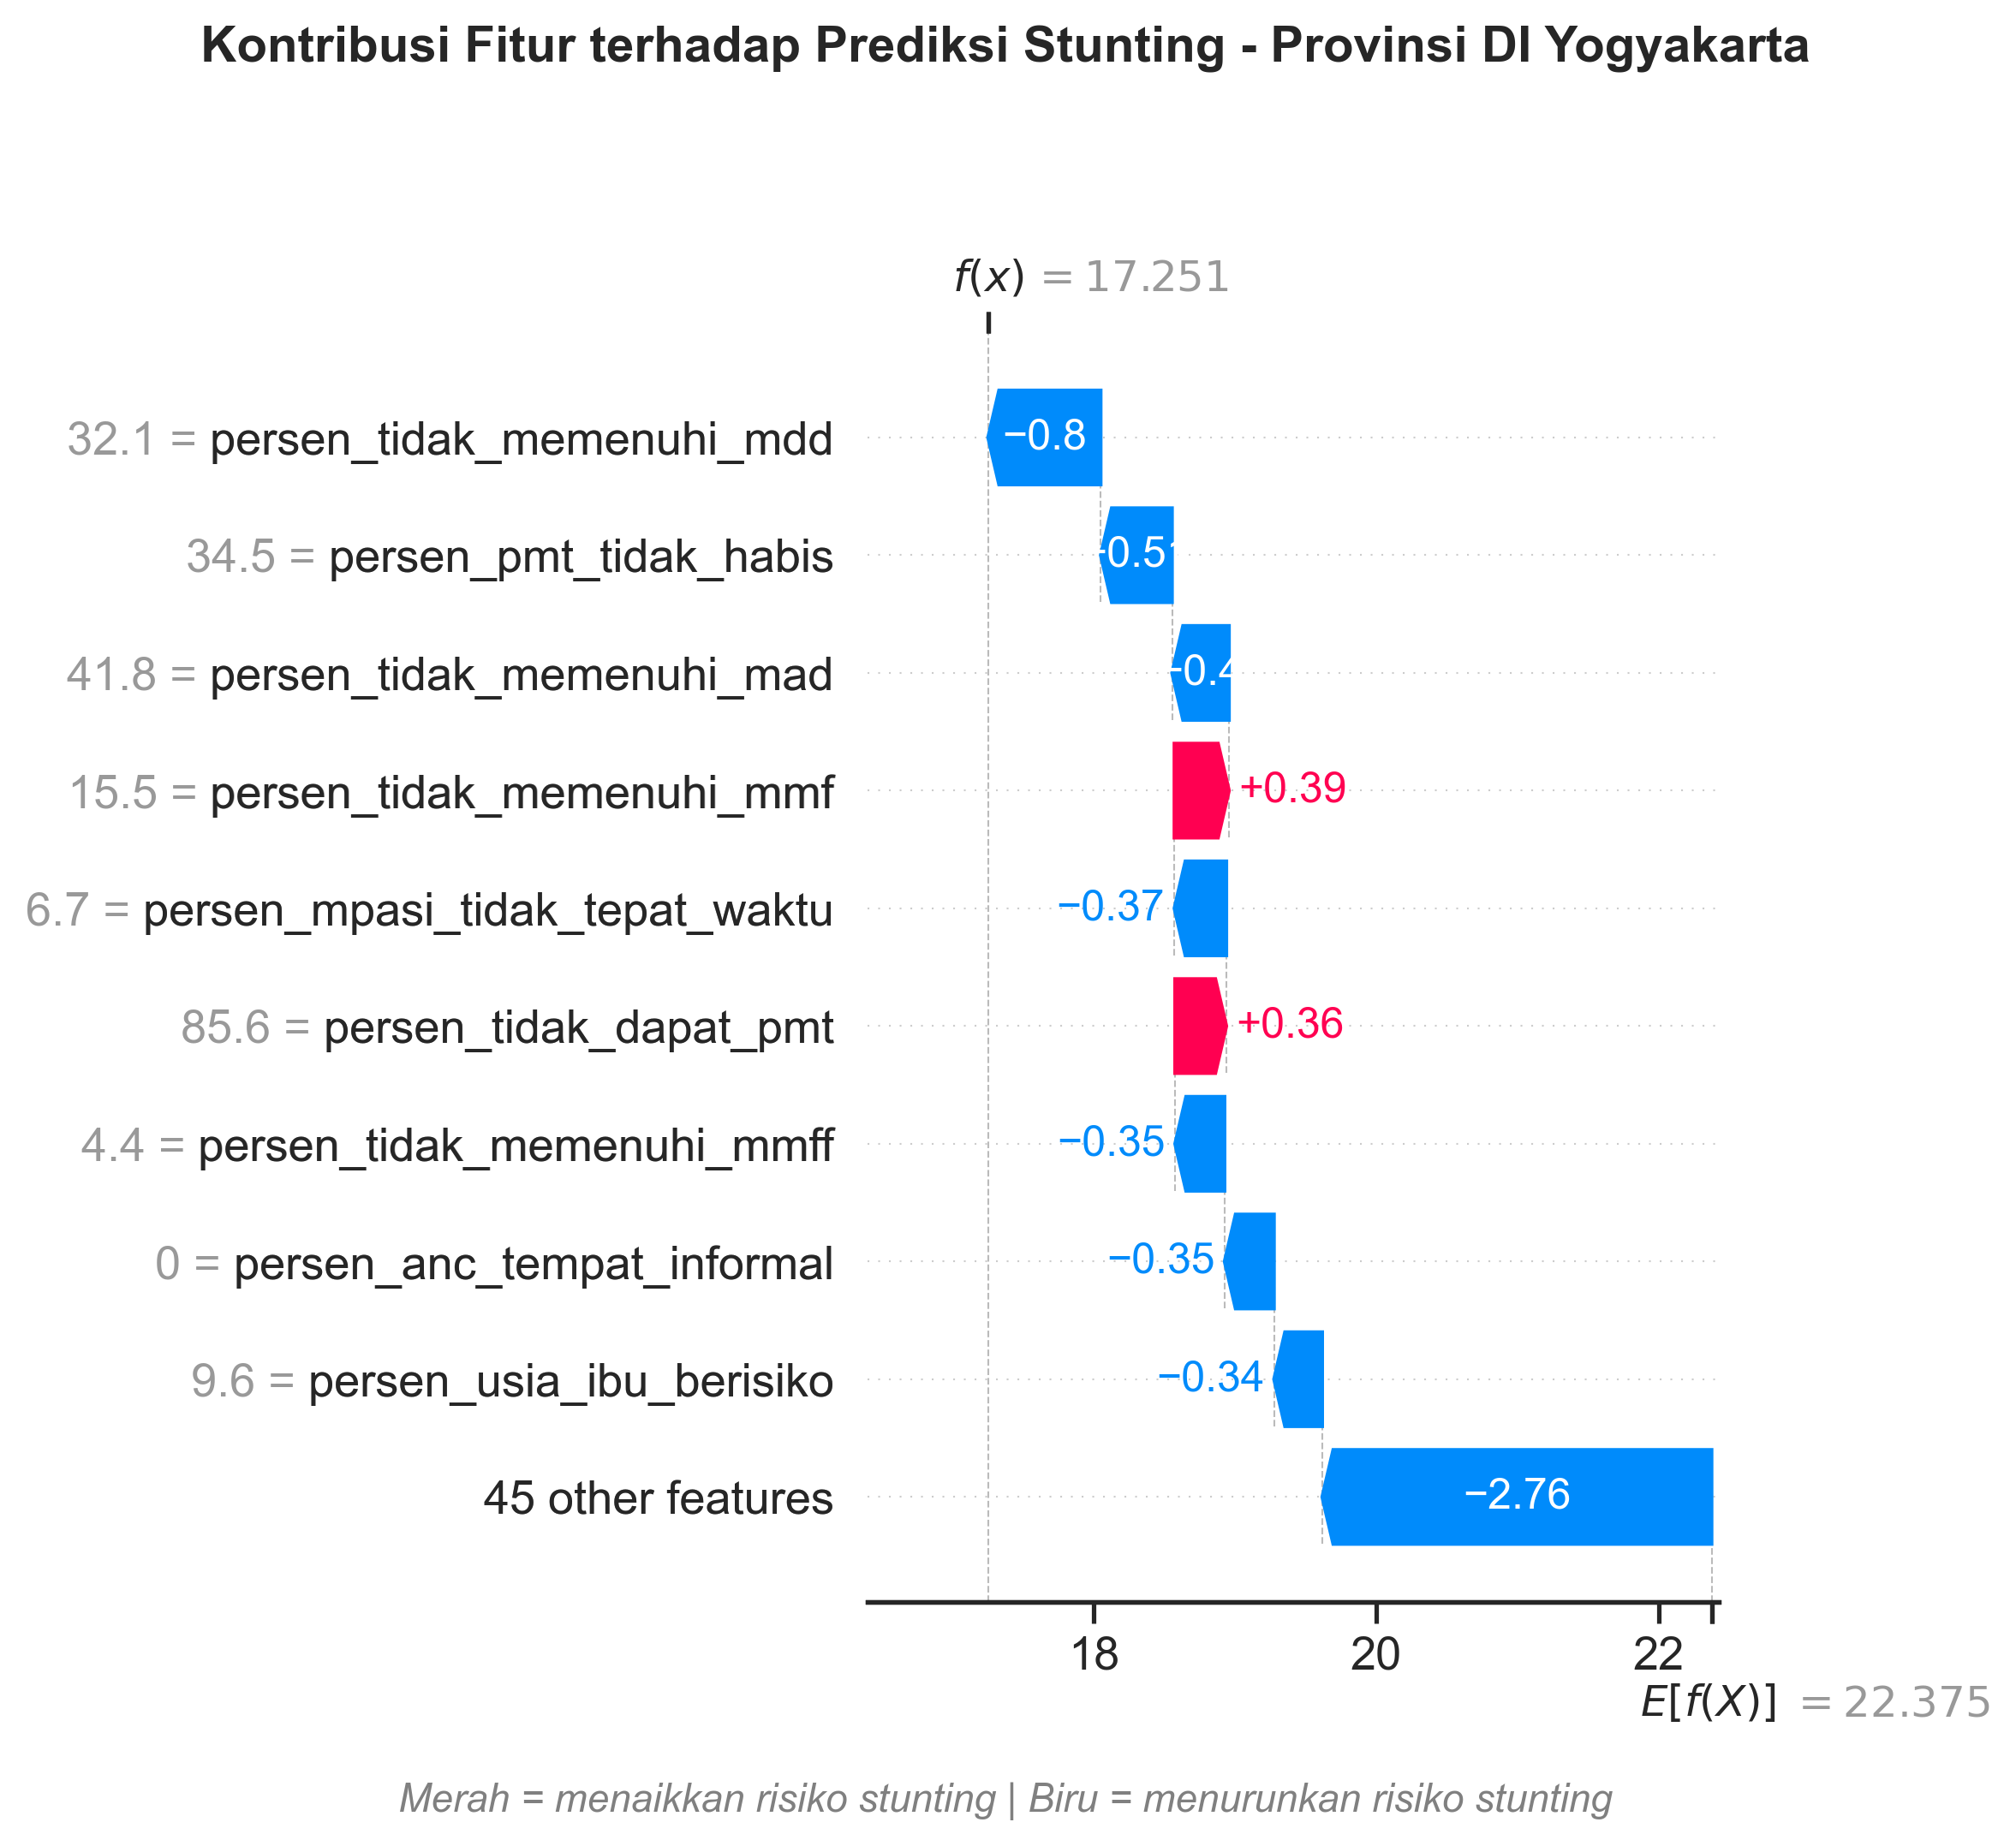
\includegraphics[width=0.48\textwidth]{figure/hasil_waterfall_stunting/waterfall_DI_Yogyakarta.png} \\ \vspace{0.5cm}
    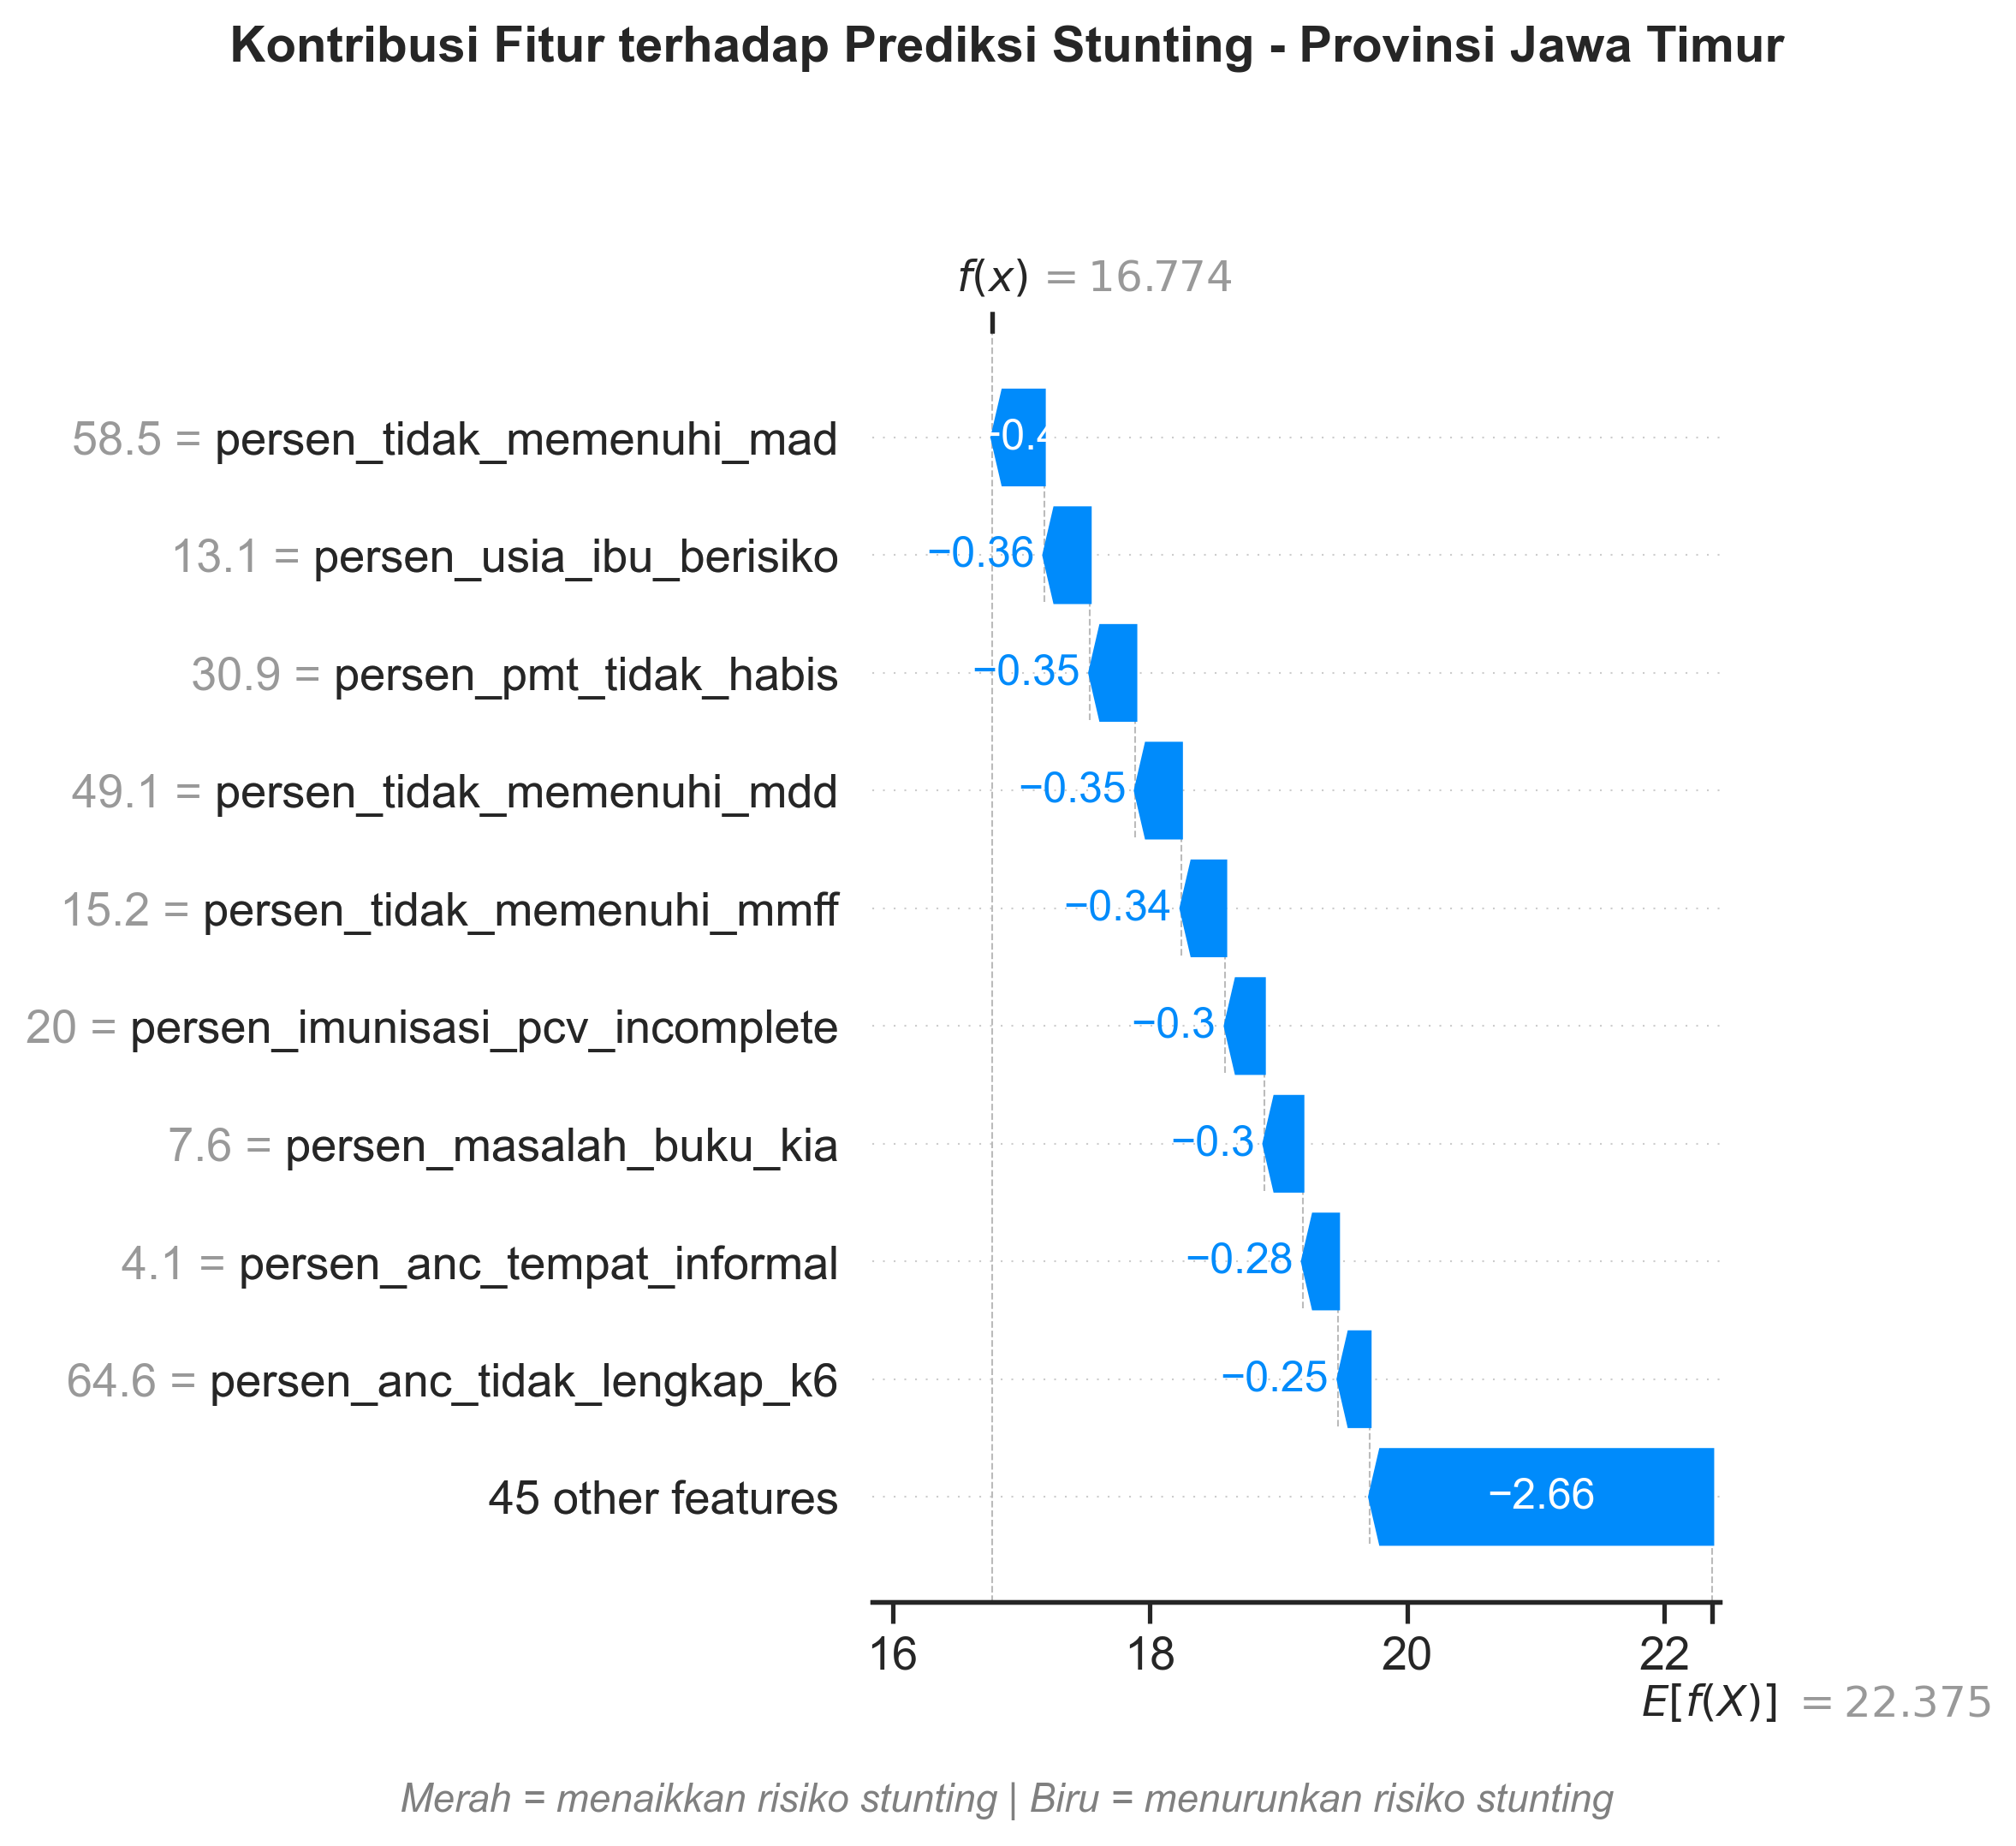
\includegraphics[width=0.48\textwidth]{figure/hasil_waterfall_stunting/waterfall_Jawa_Timur.png} \hfill
    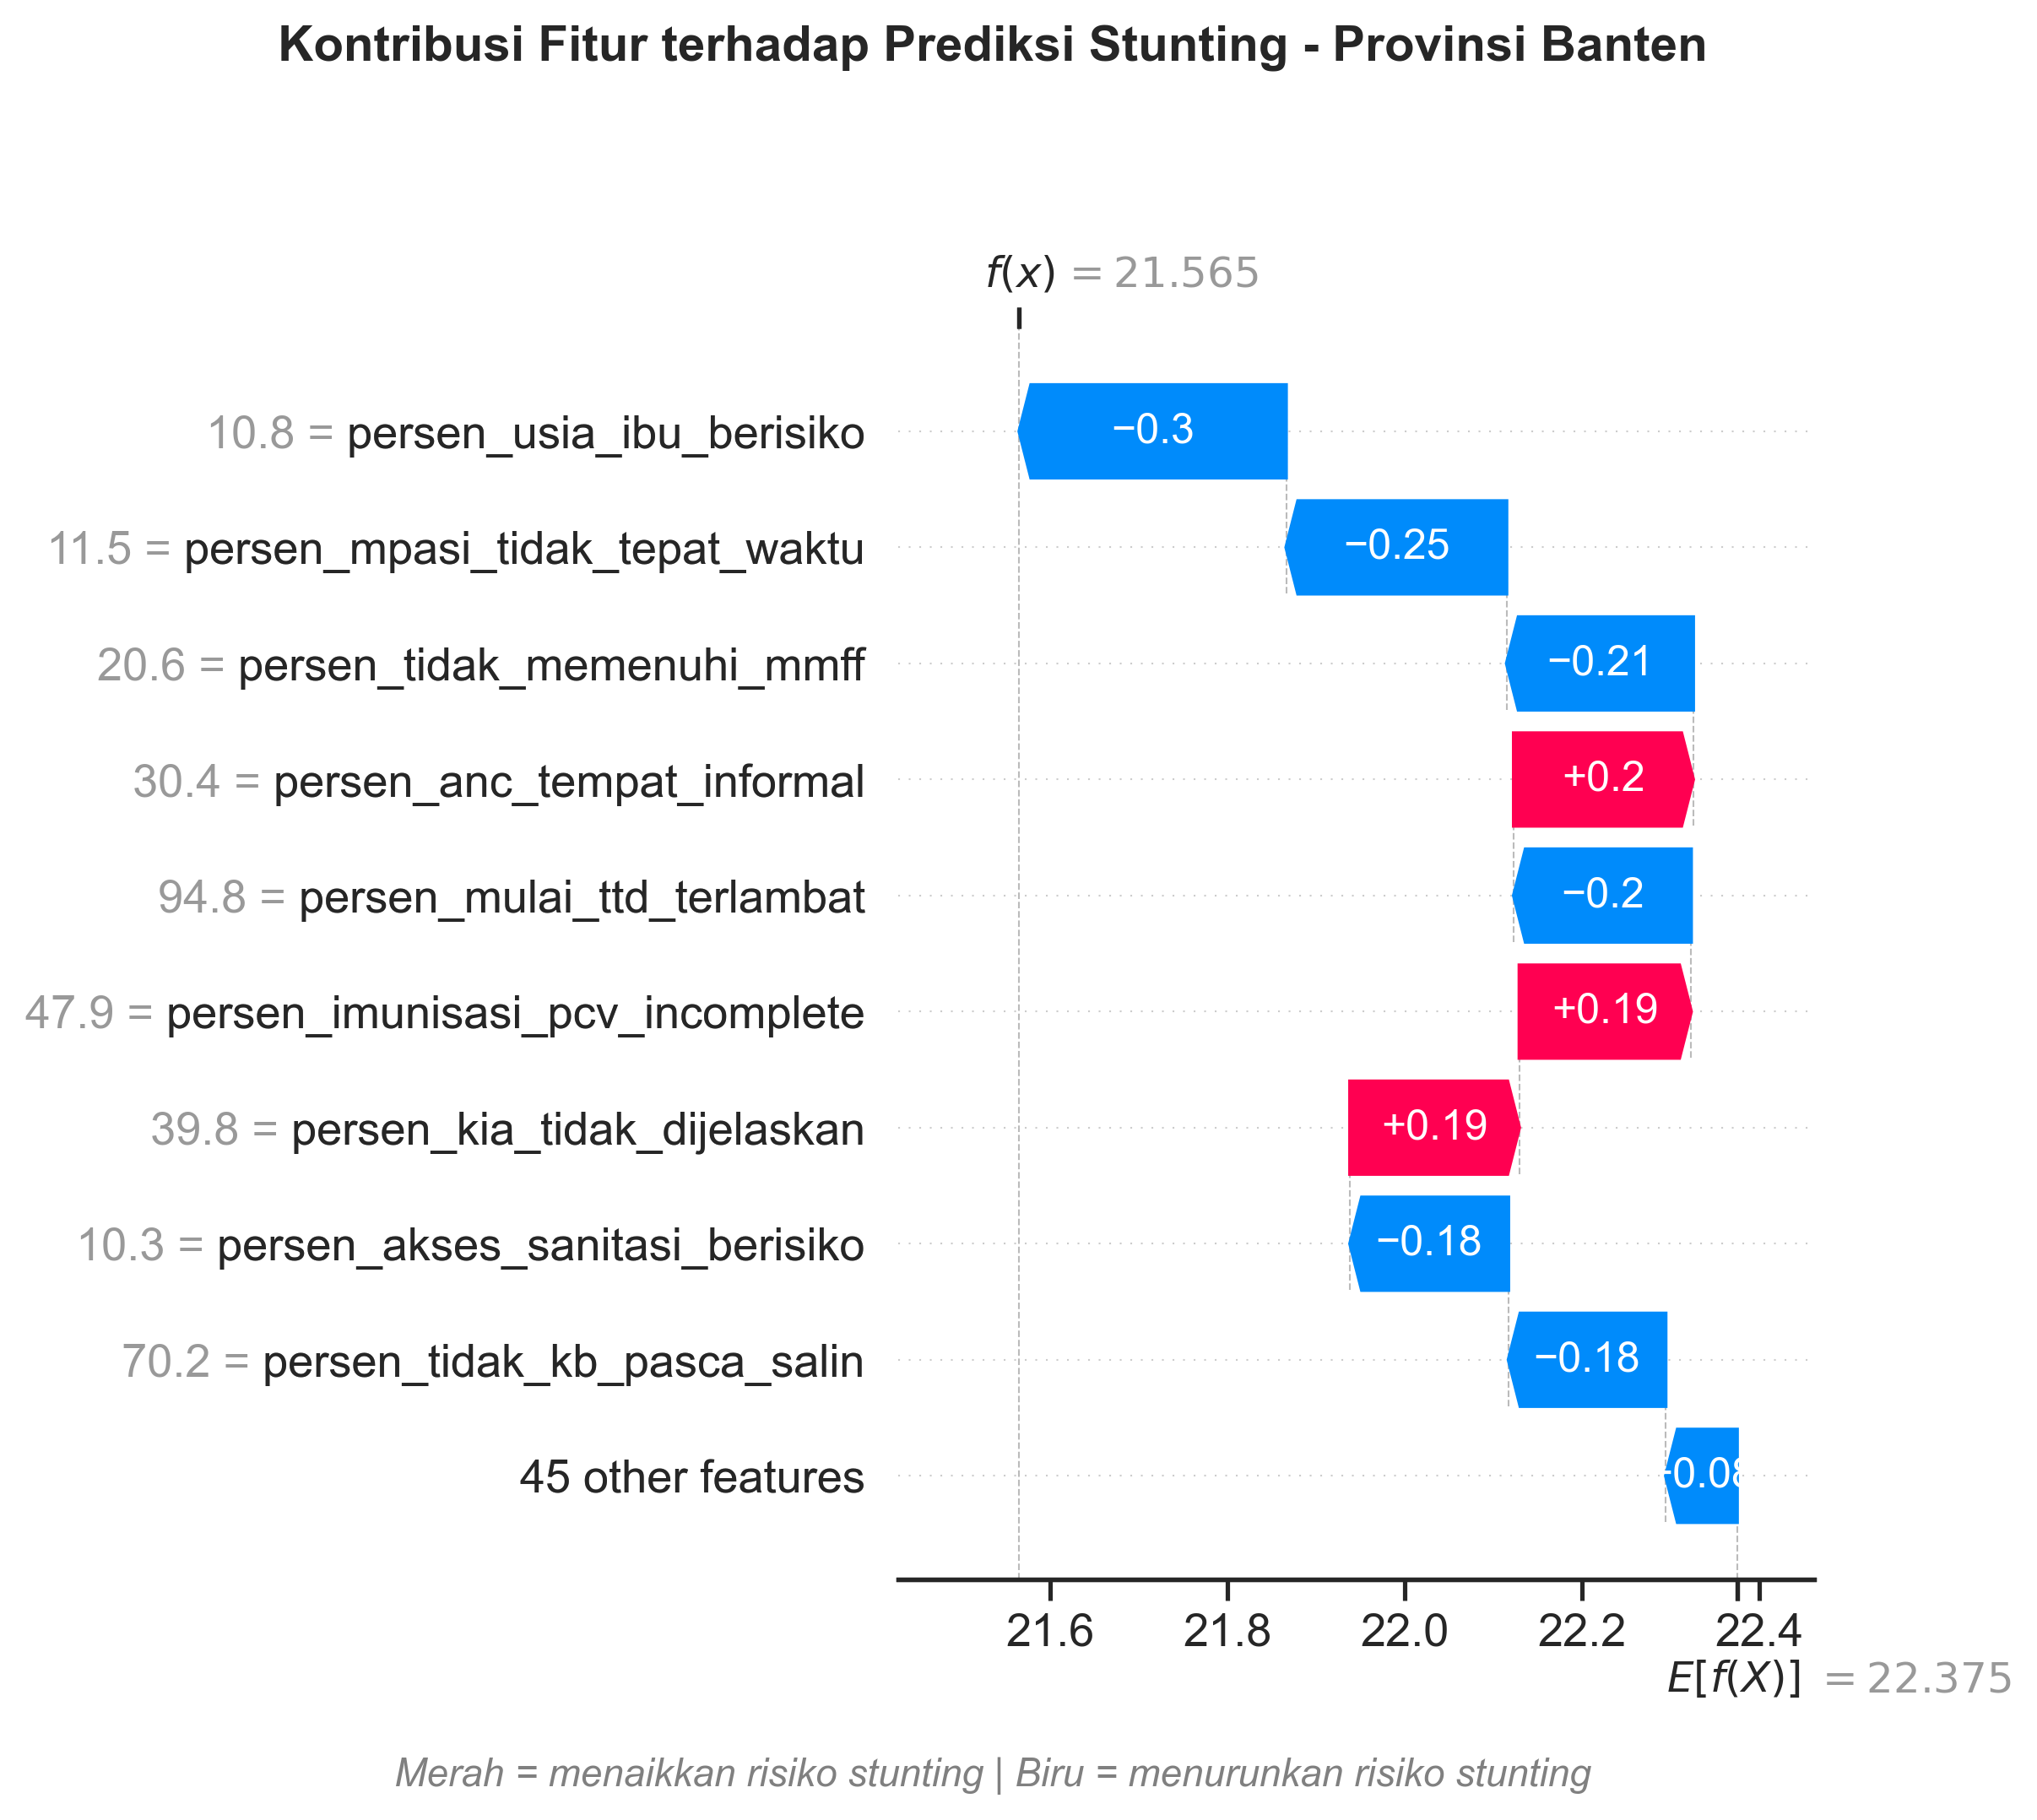
\includegraphics[width=0.48\textwidth]{figure/hasil_waterfall_stunting/waterfall_Banten.png} \\ \vspace{0.5cm}
    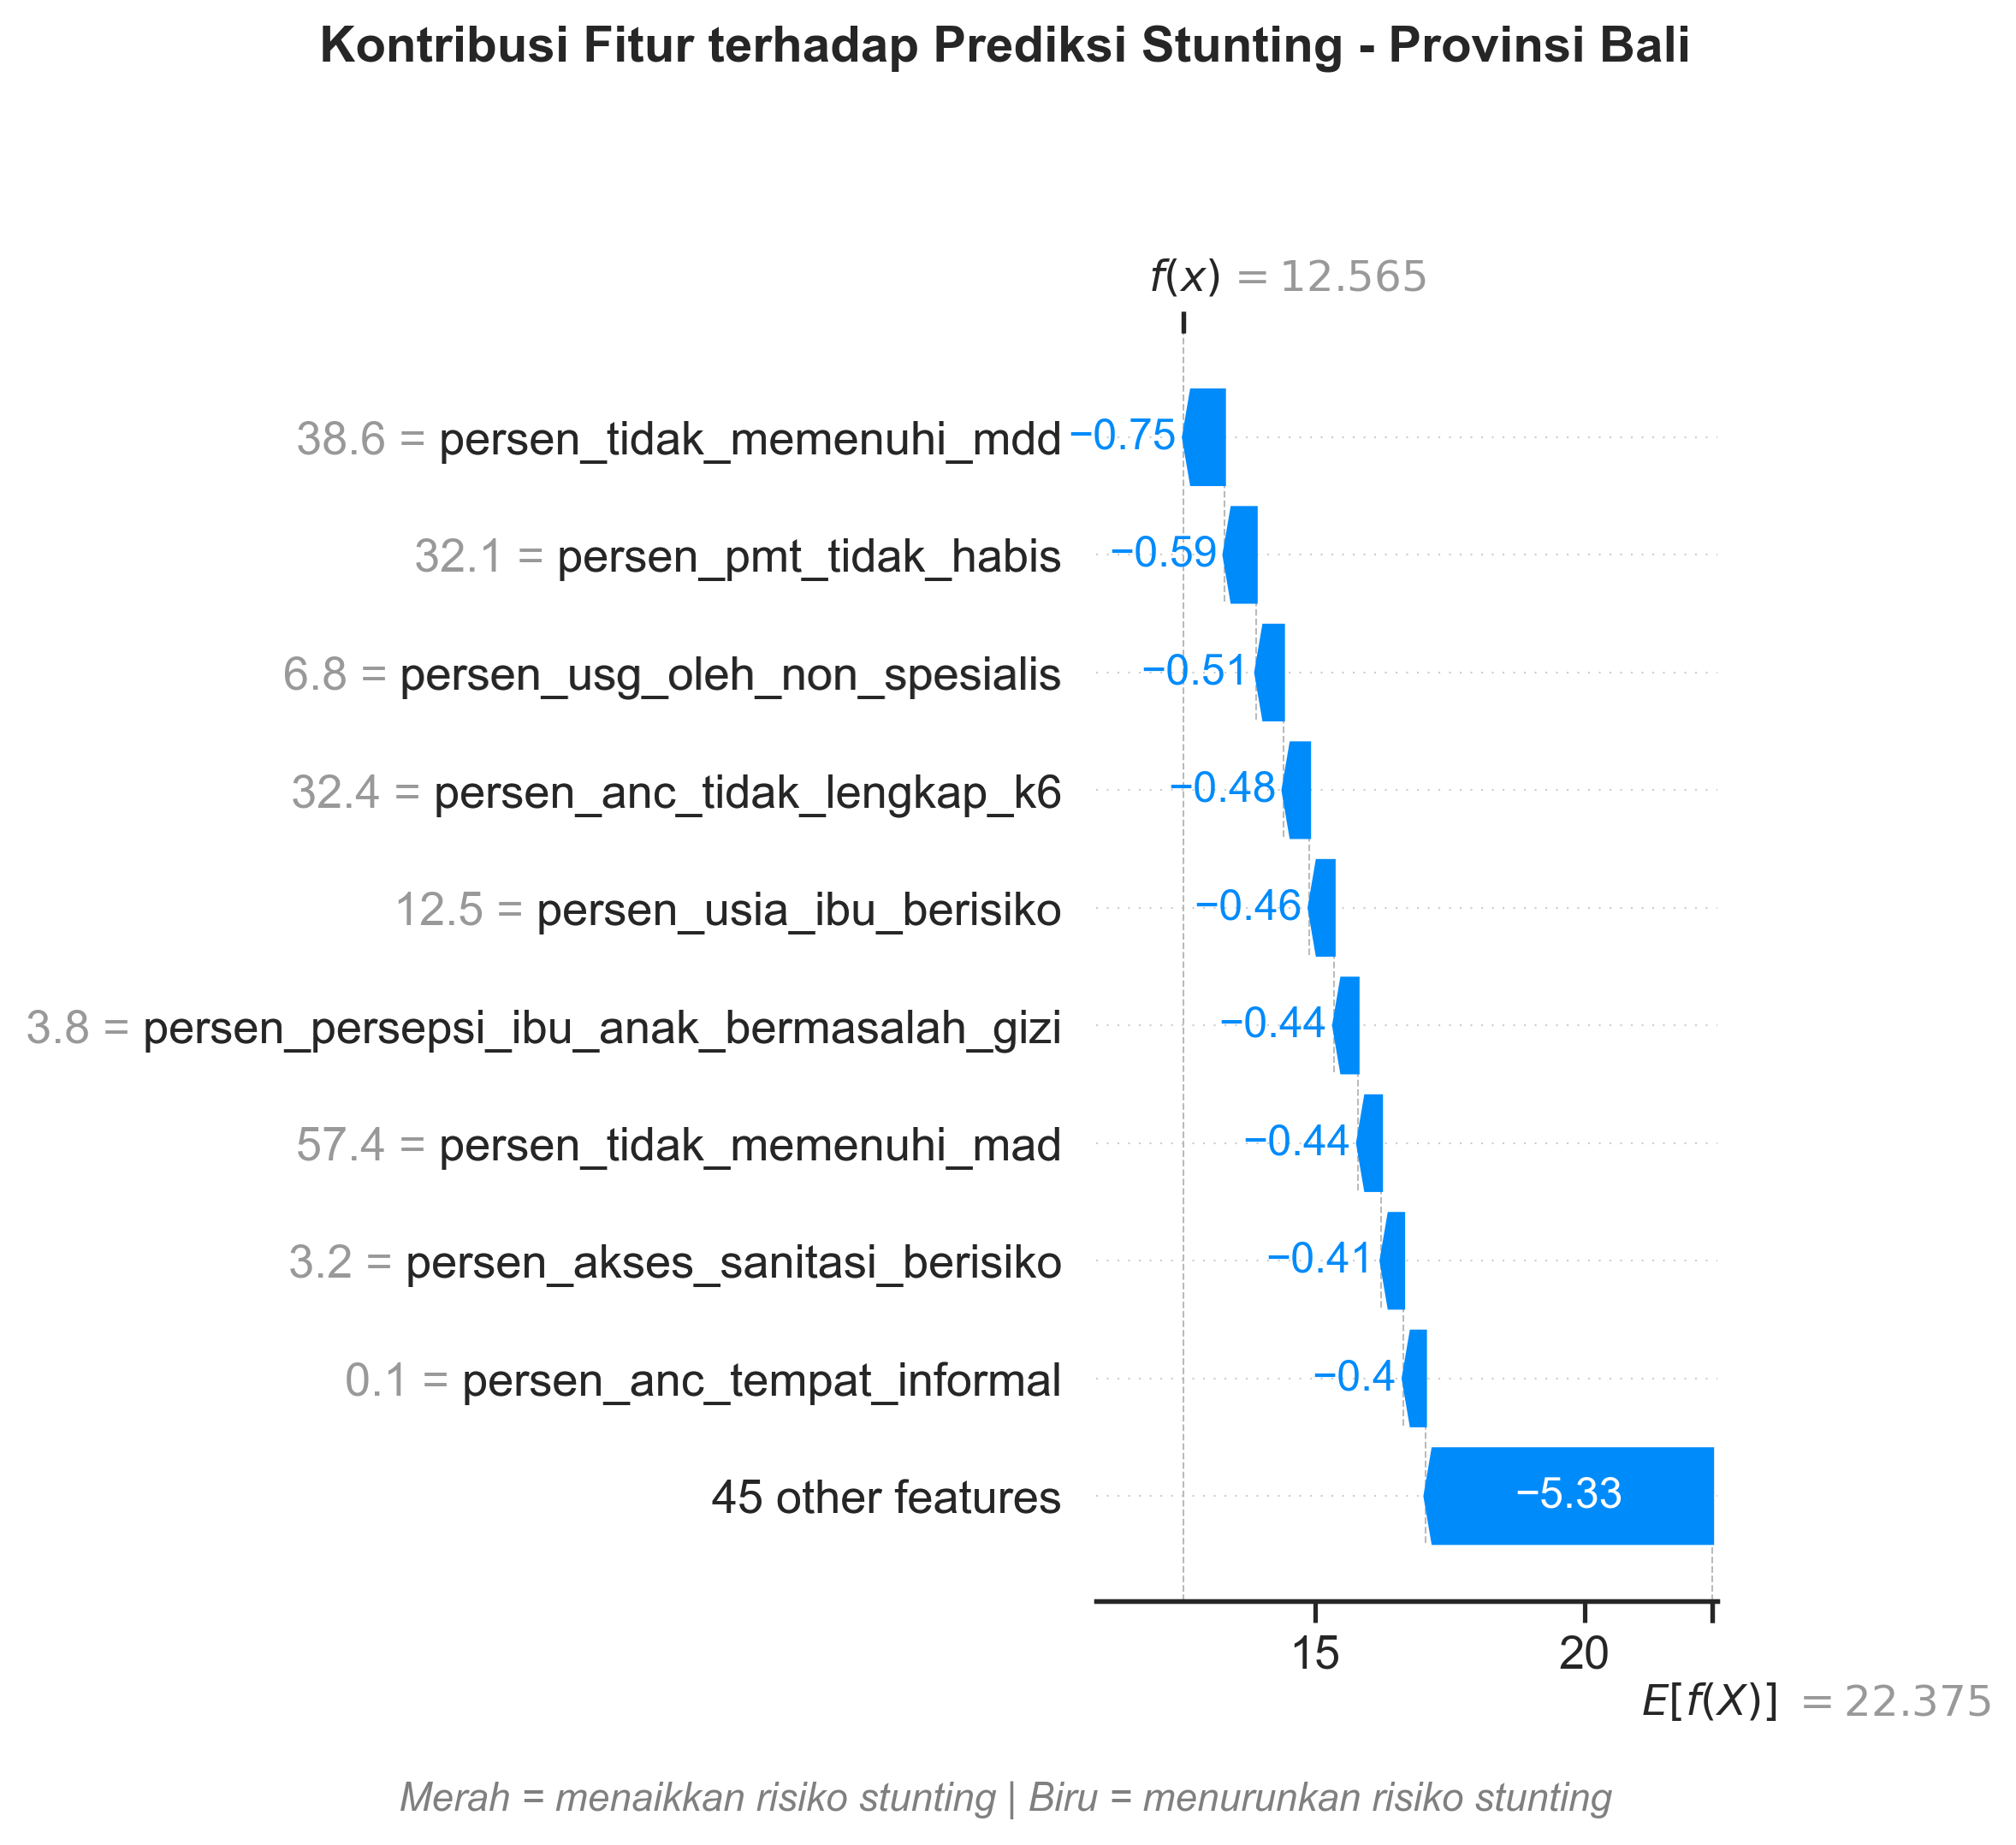
\includegraphics[width=0.48\textwidth]{figure/hasil_waterfall_stunting/waterfall_Bali.png} \hfill
    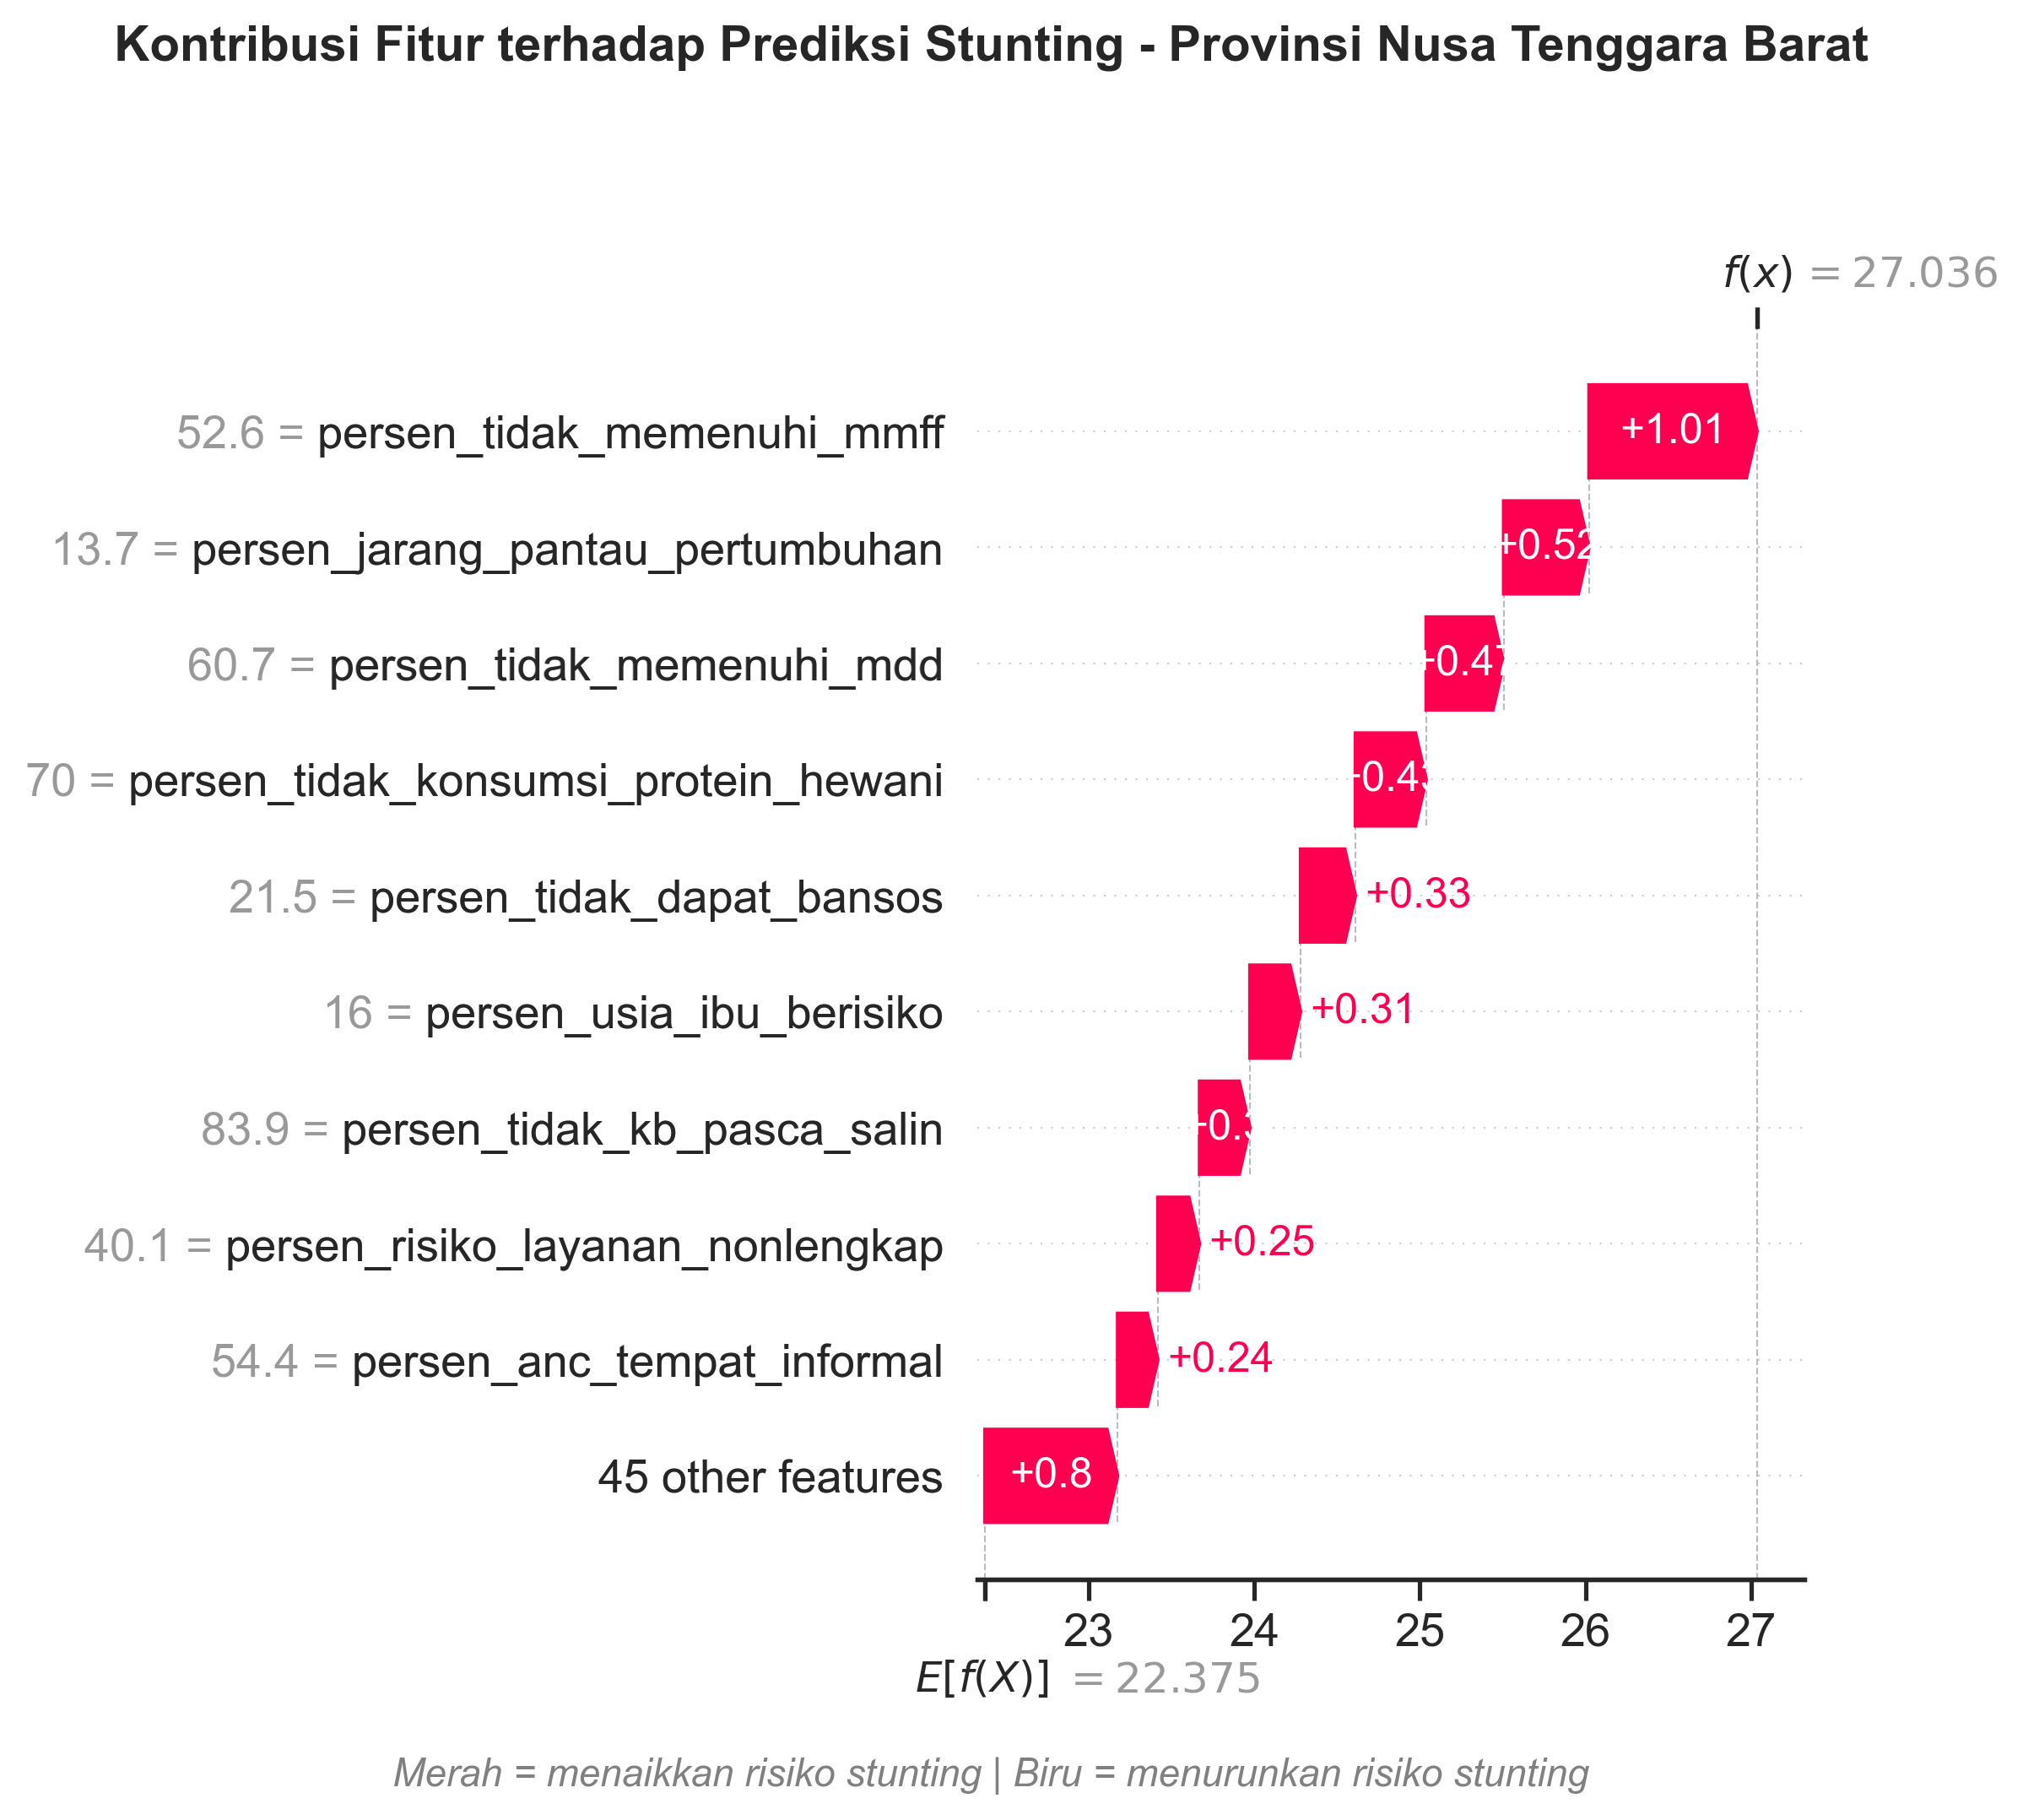
\includegraphics[width=0.48\textwidth]{figure/hasil_waterfall_stunting/waterfall_Nusa_Tenggara_Barat.png}
\end{figure}

\newpage
\begin{figure}[H]
    \centering
    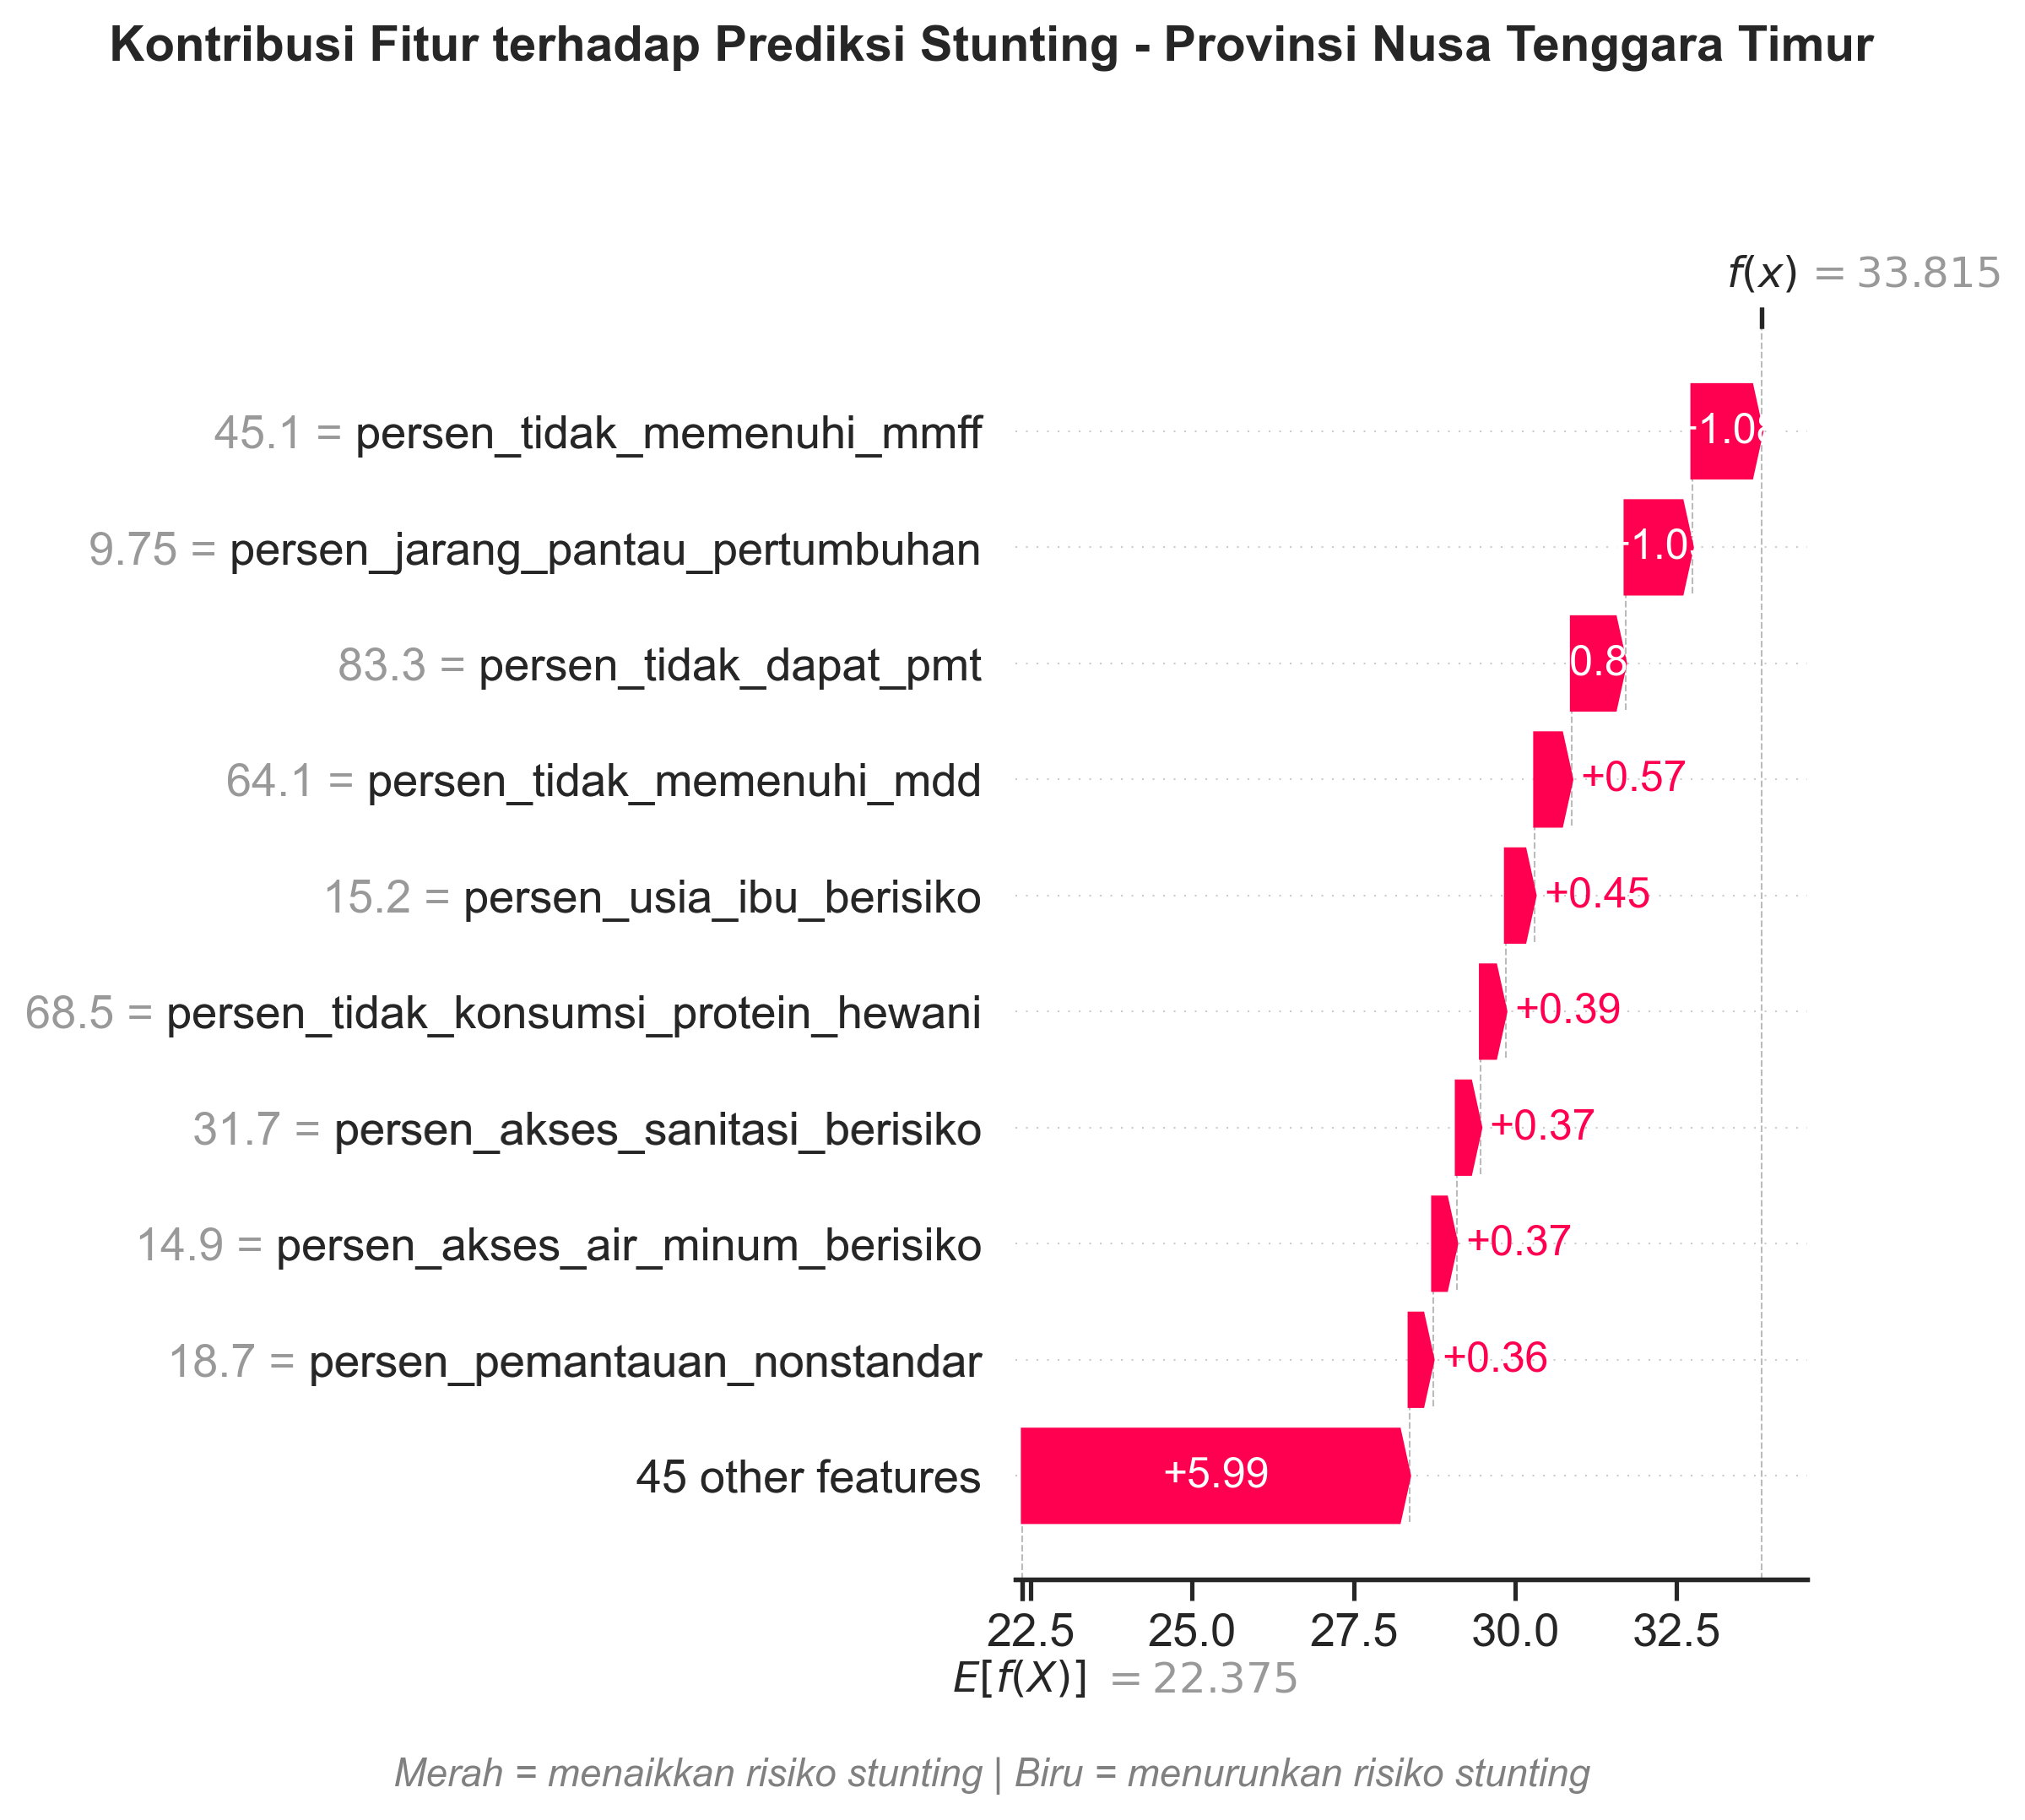
\includegraphics[width=0.48\textwidth]{figure/hasil_waterfall_stunting/waterfall_Nusa_Tenggara_Timur.png} \hfill
    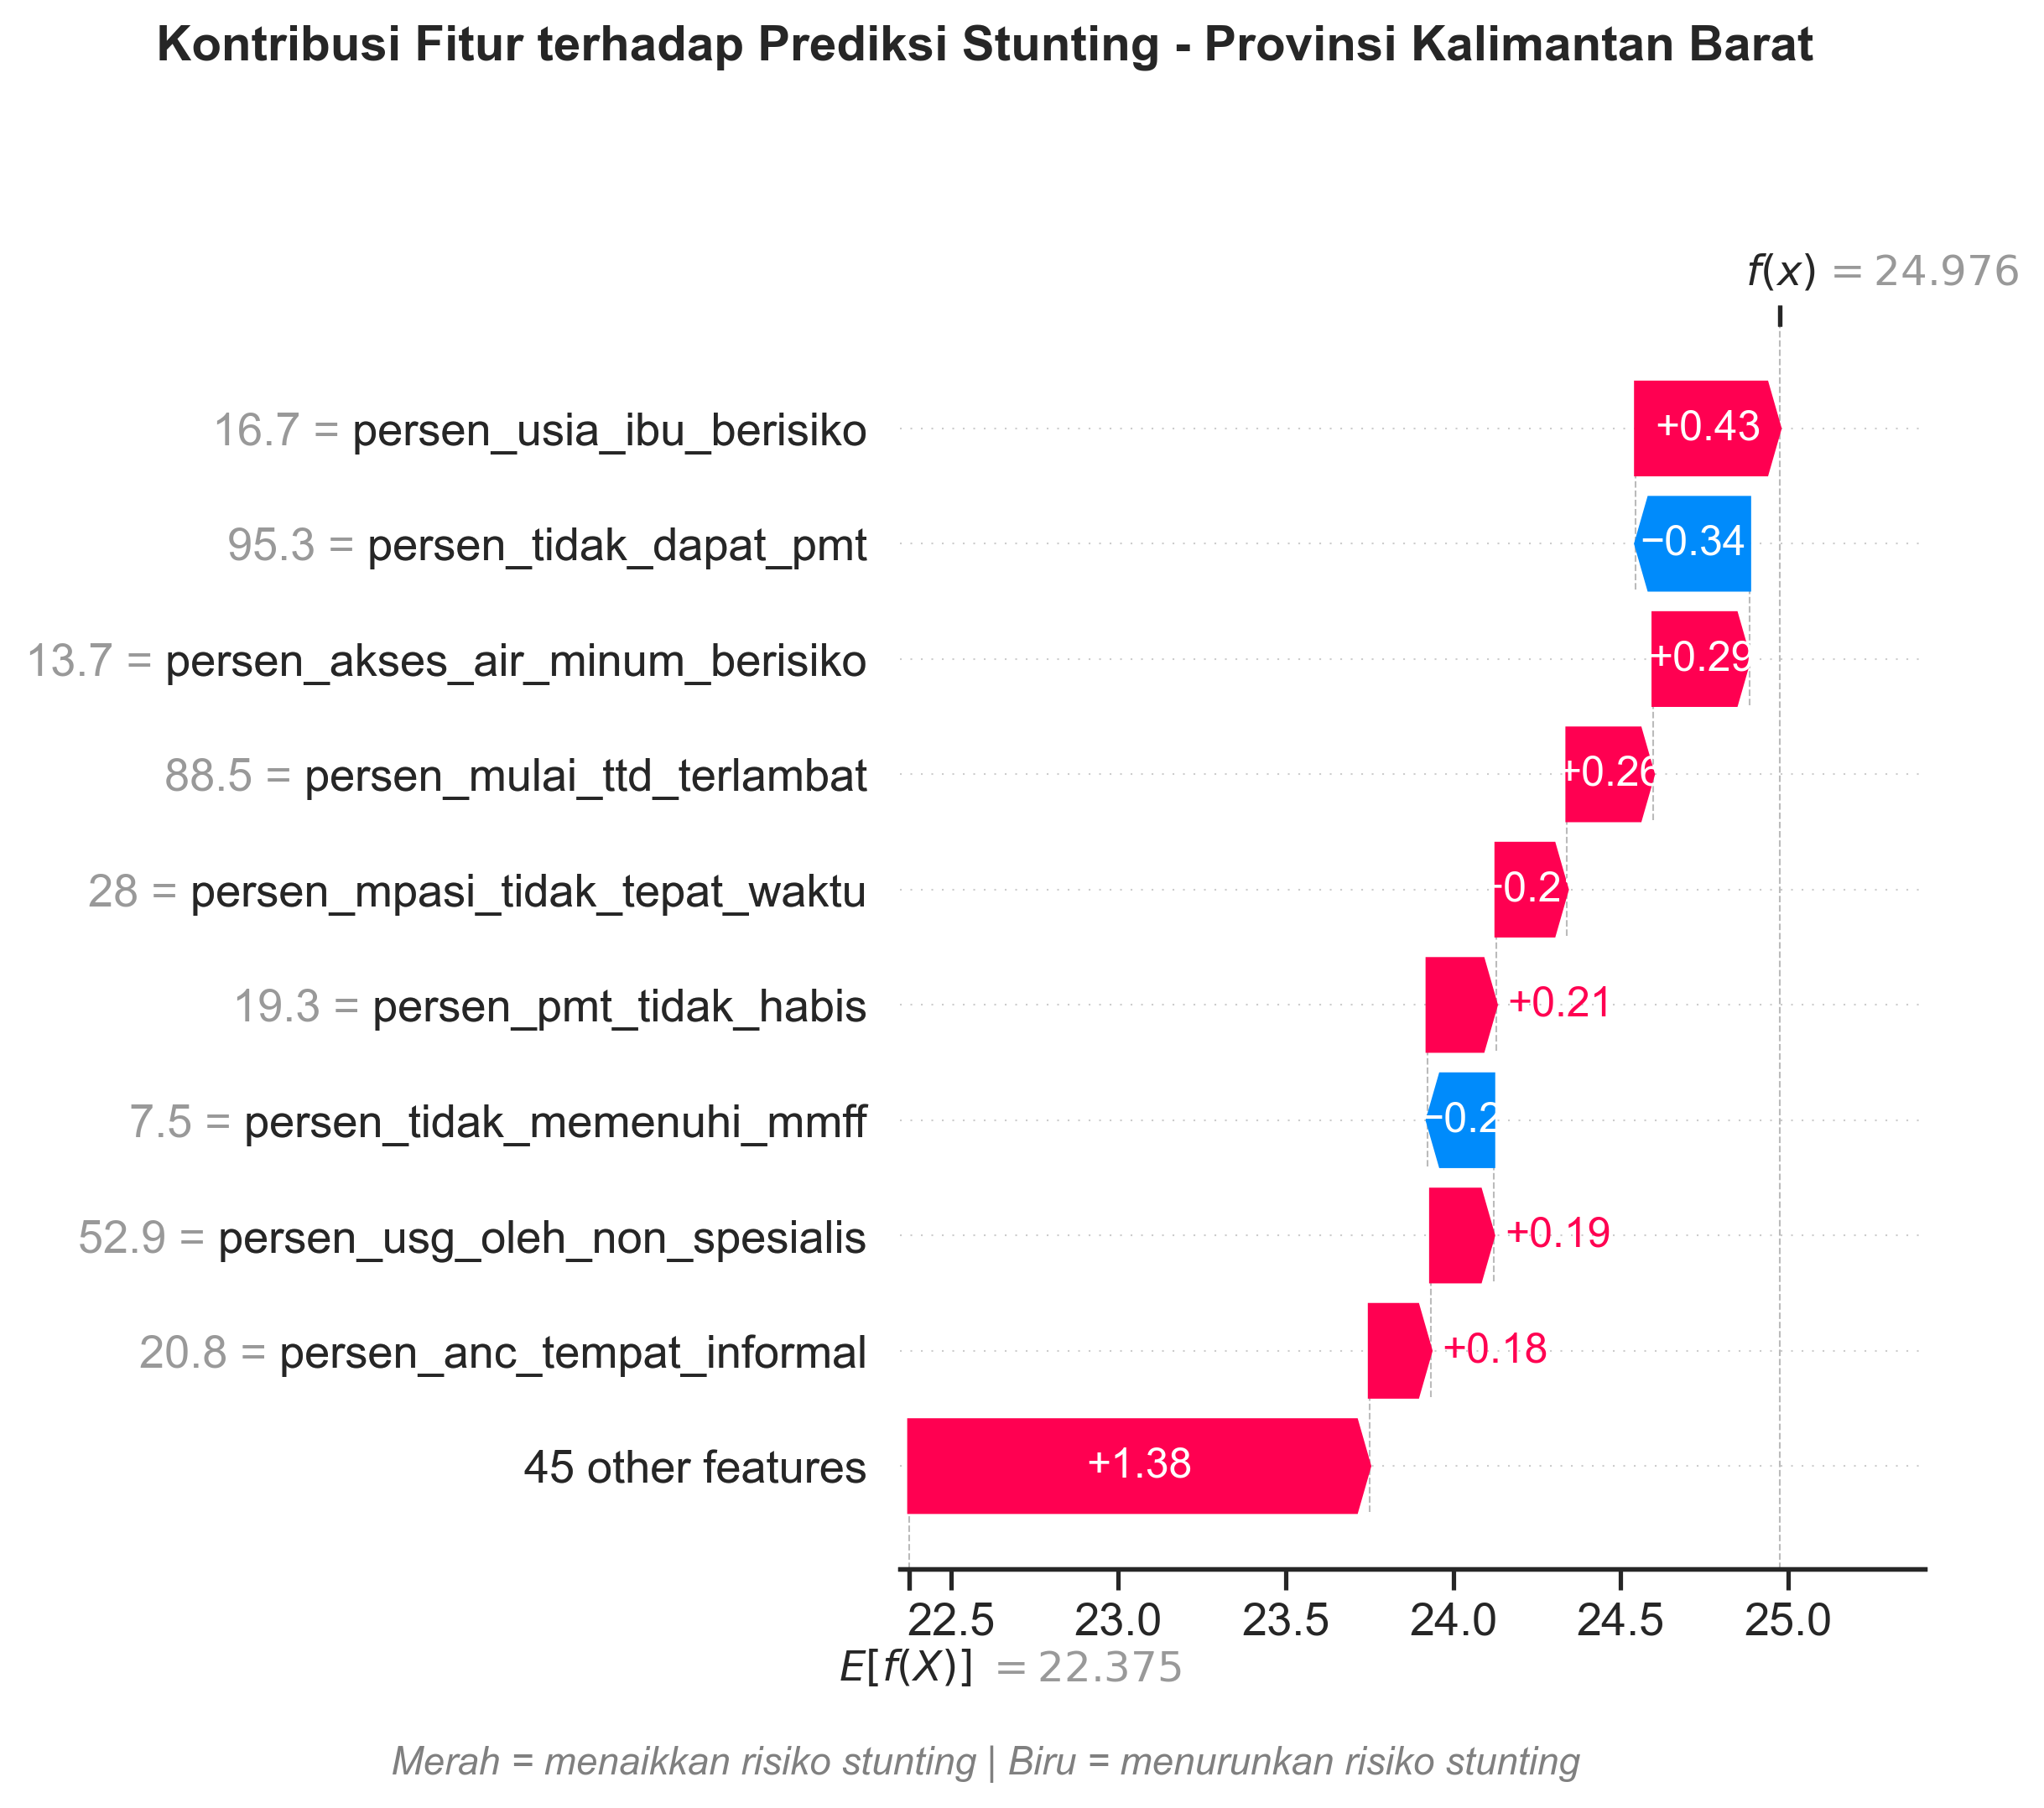
\includegraphics[width=0.48\textwidth]{figure/hasil_waterfall_stunting/waterfall_Kalimantan_Barat.png} \\ \vspace{0.5cm}
    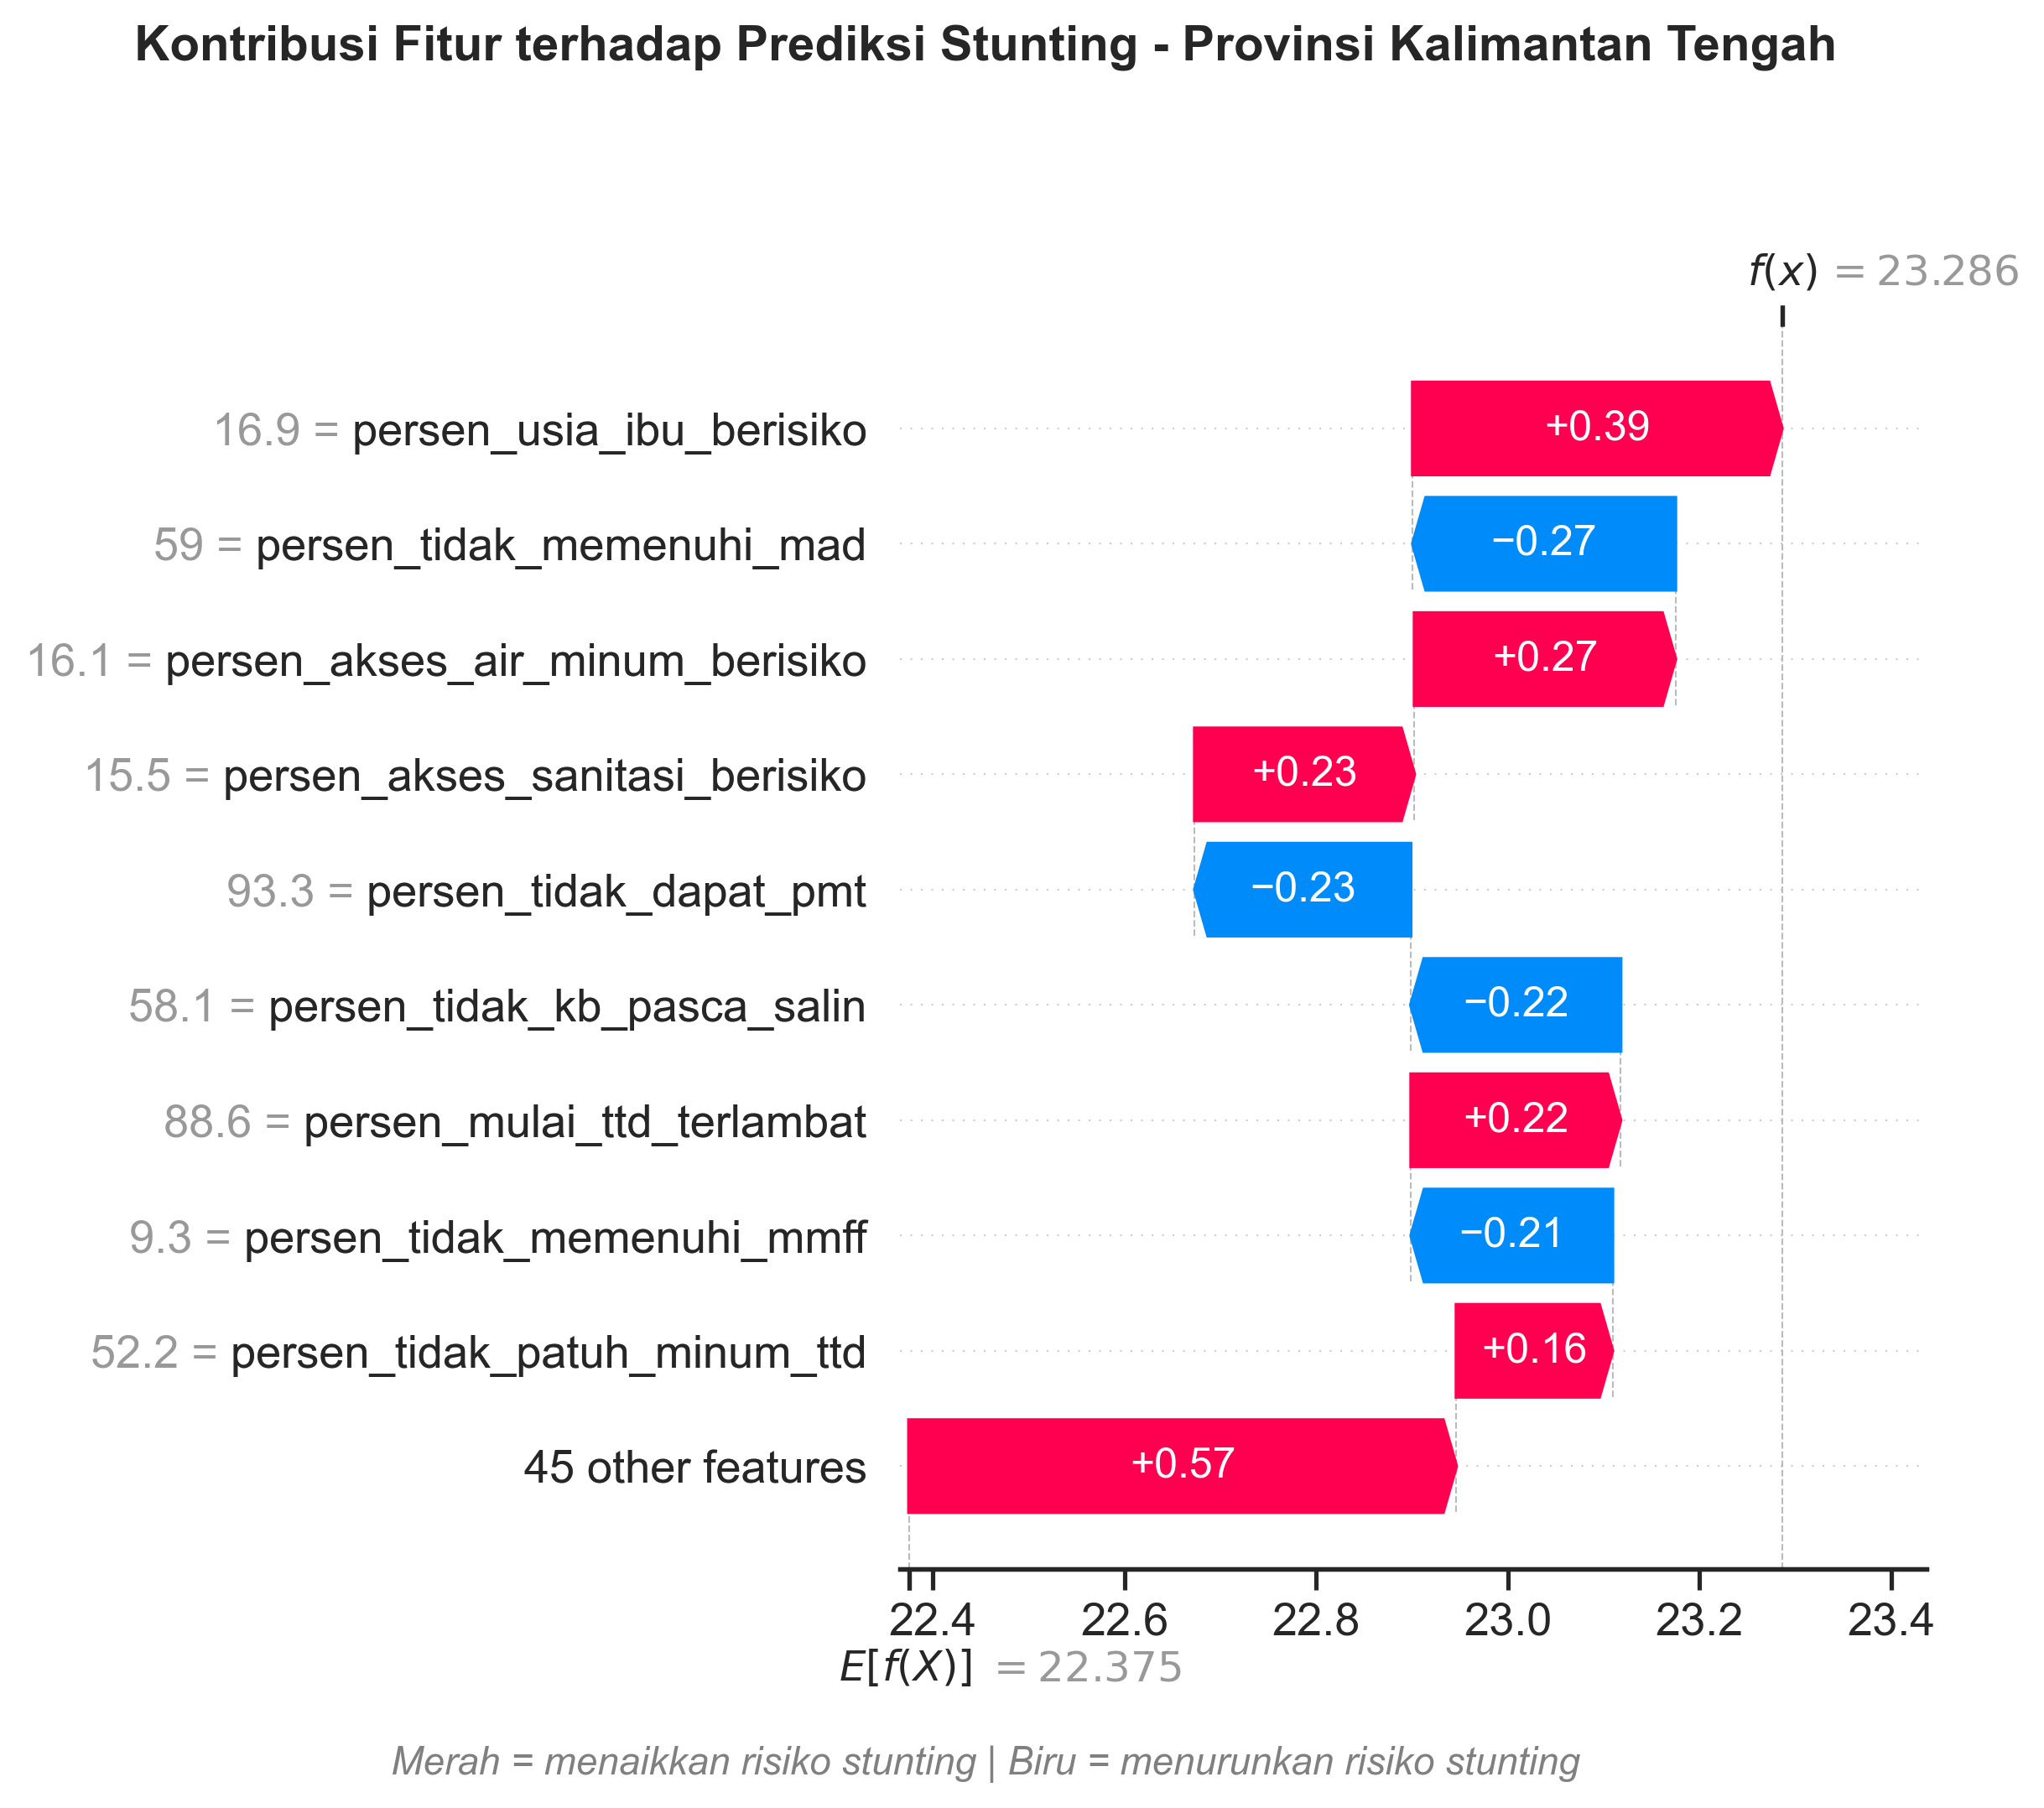
\includegraphics[width=0.48\textwidth]{figure/hasil_waterfall_stunting/waterfall_Kalimantan_Tengah.png} \hfill
    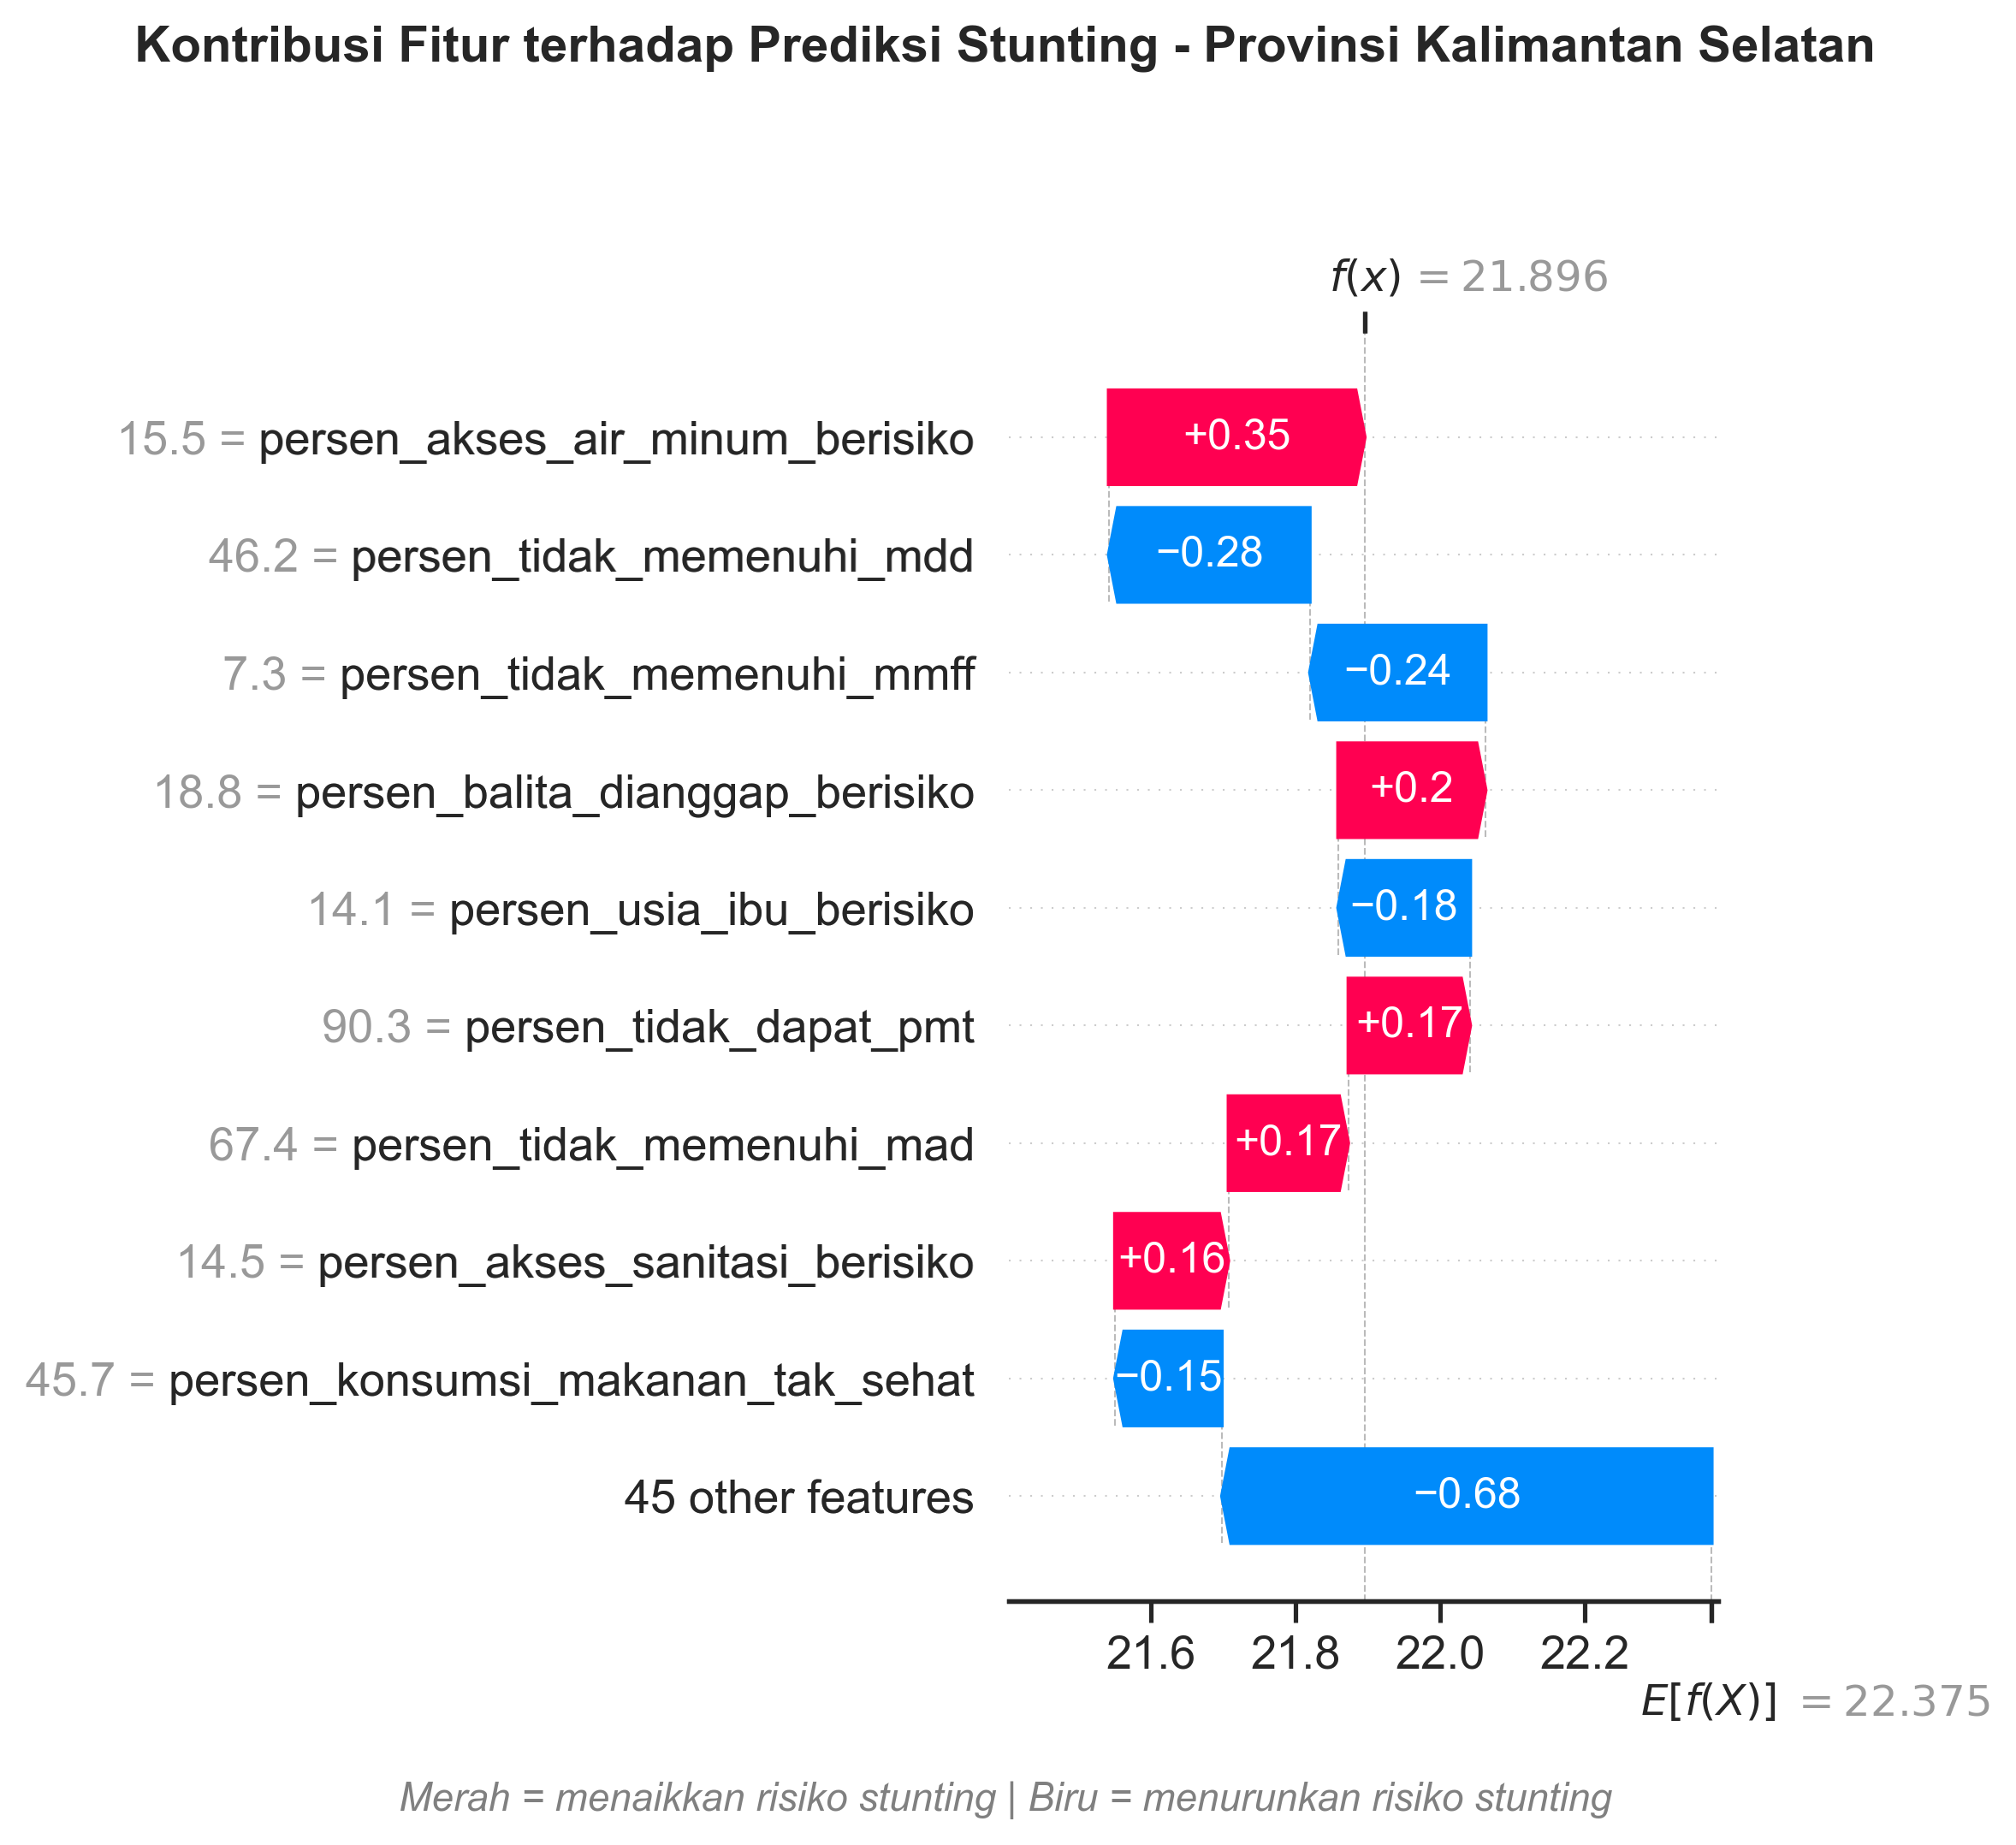
\includegraphics[width=0.48\textwidth]{figure/hasil_waterfall_stunting/waterfall_Kalimantan_Selatan.png} \\ \vspace{0.5cm}
    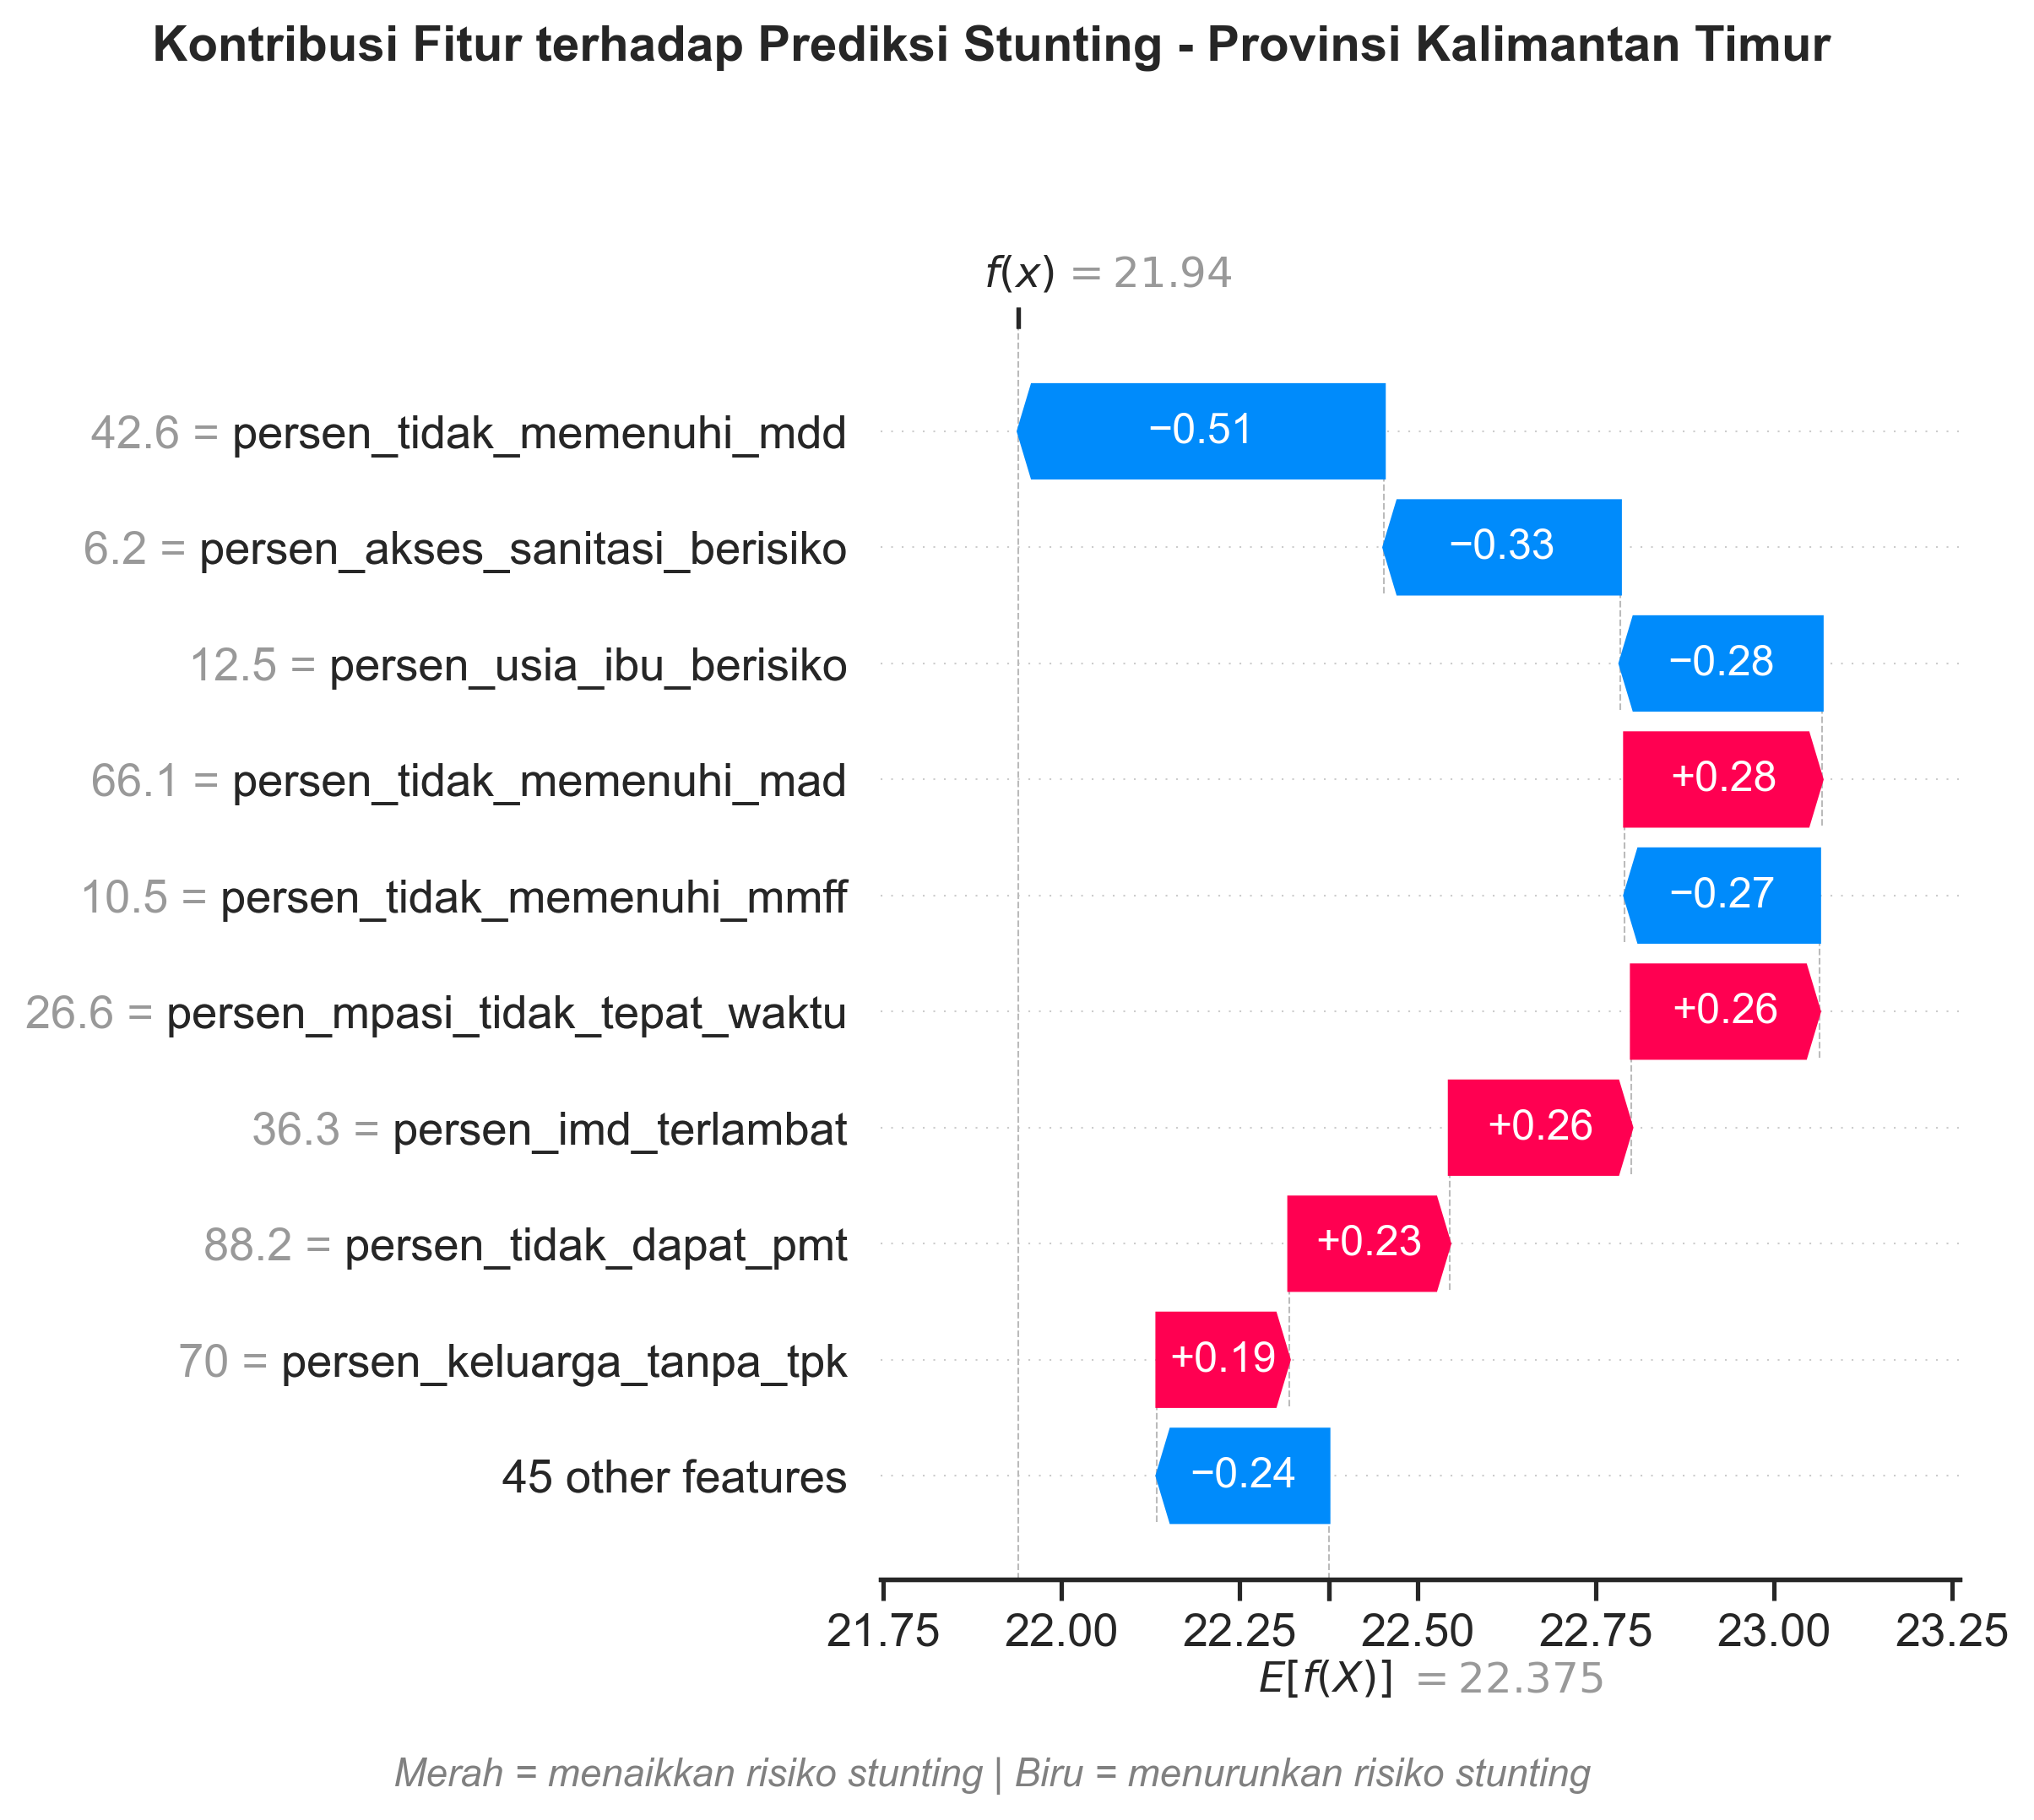
\includegraphics[width=0.48\textwidth]{figure/hasil_waterfall_stunting/waterfall_Kalimantan_Timur.png} \hfill
    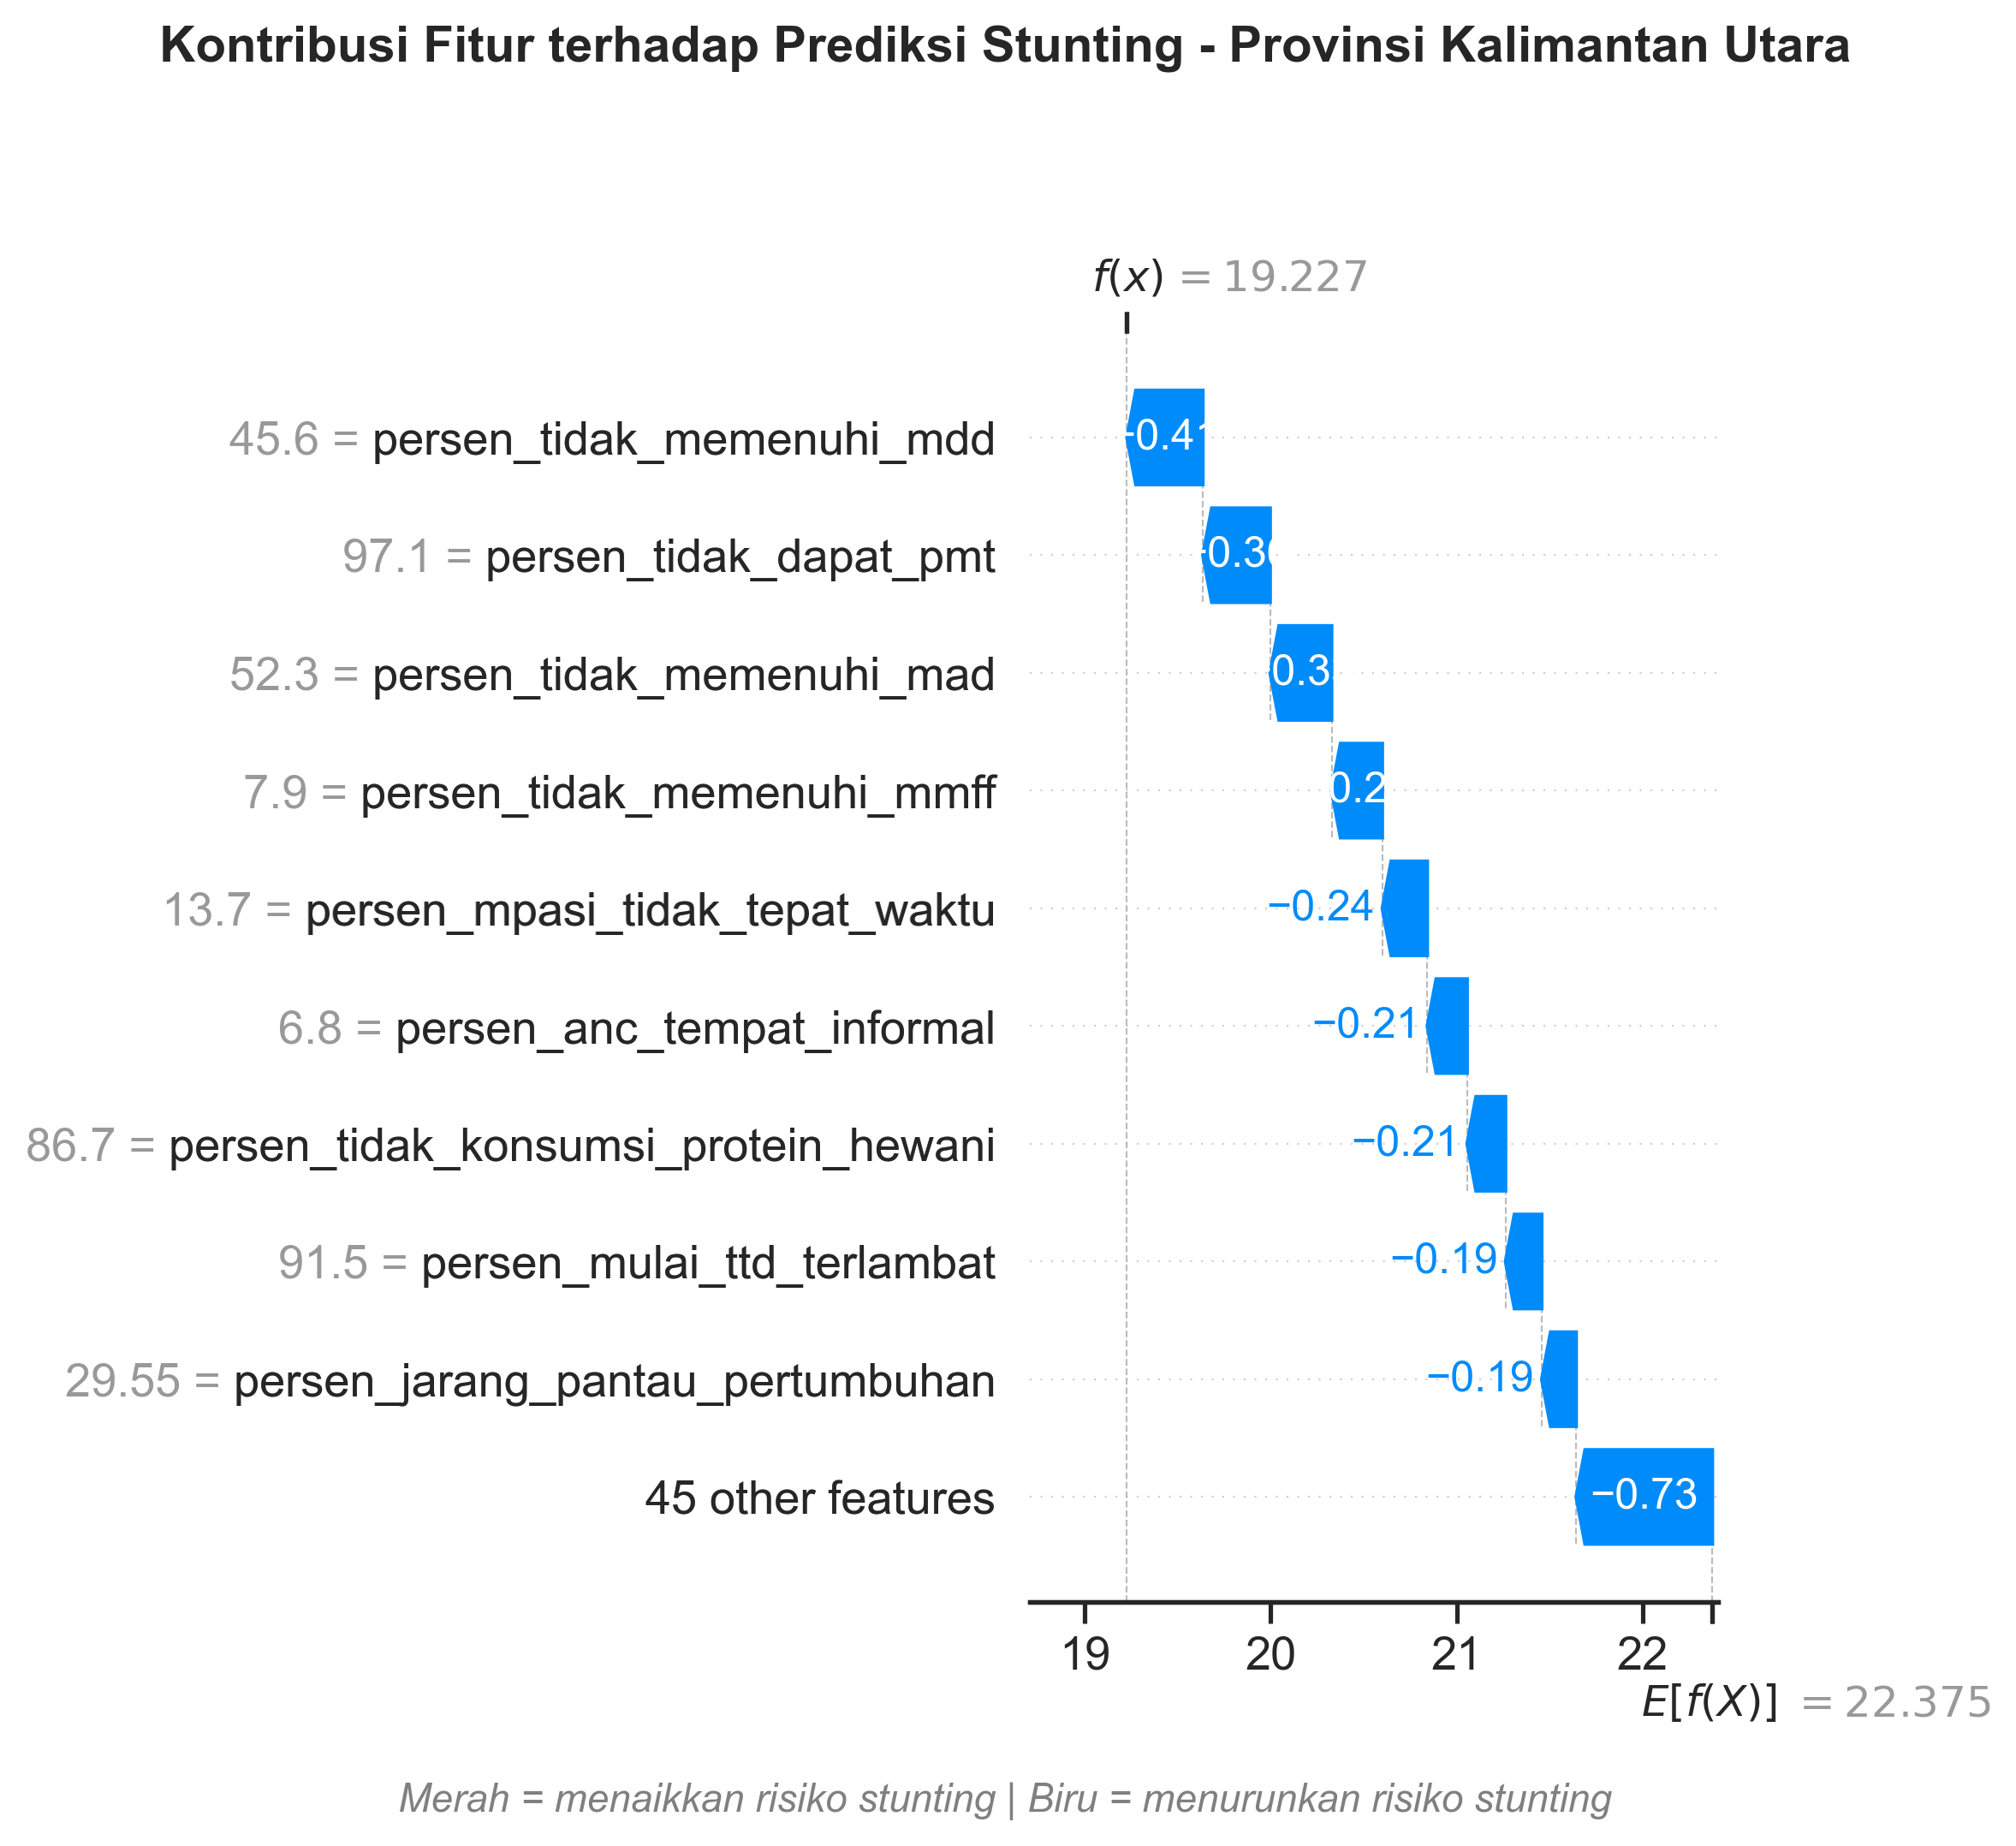
\includegraphics[width=0.48\textwidth]{figure/hasil_waterfall_stunting/waterfall_Kalimantan_Utara.png}
\end{figure}

\newpage
\begin{figure}[H]
    \centering
    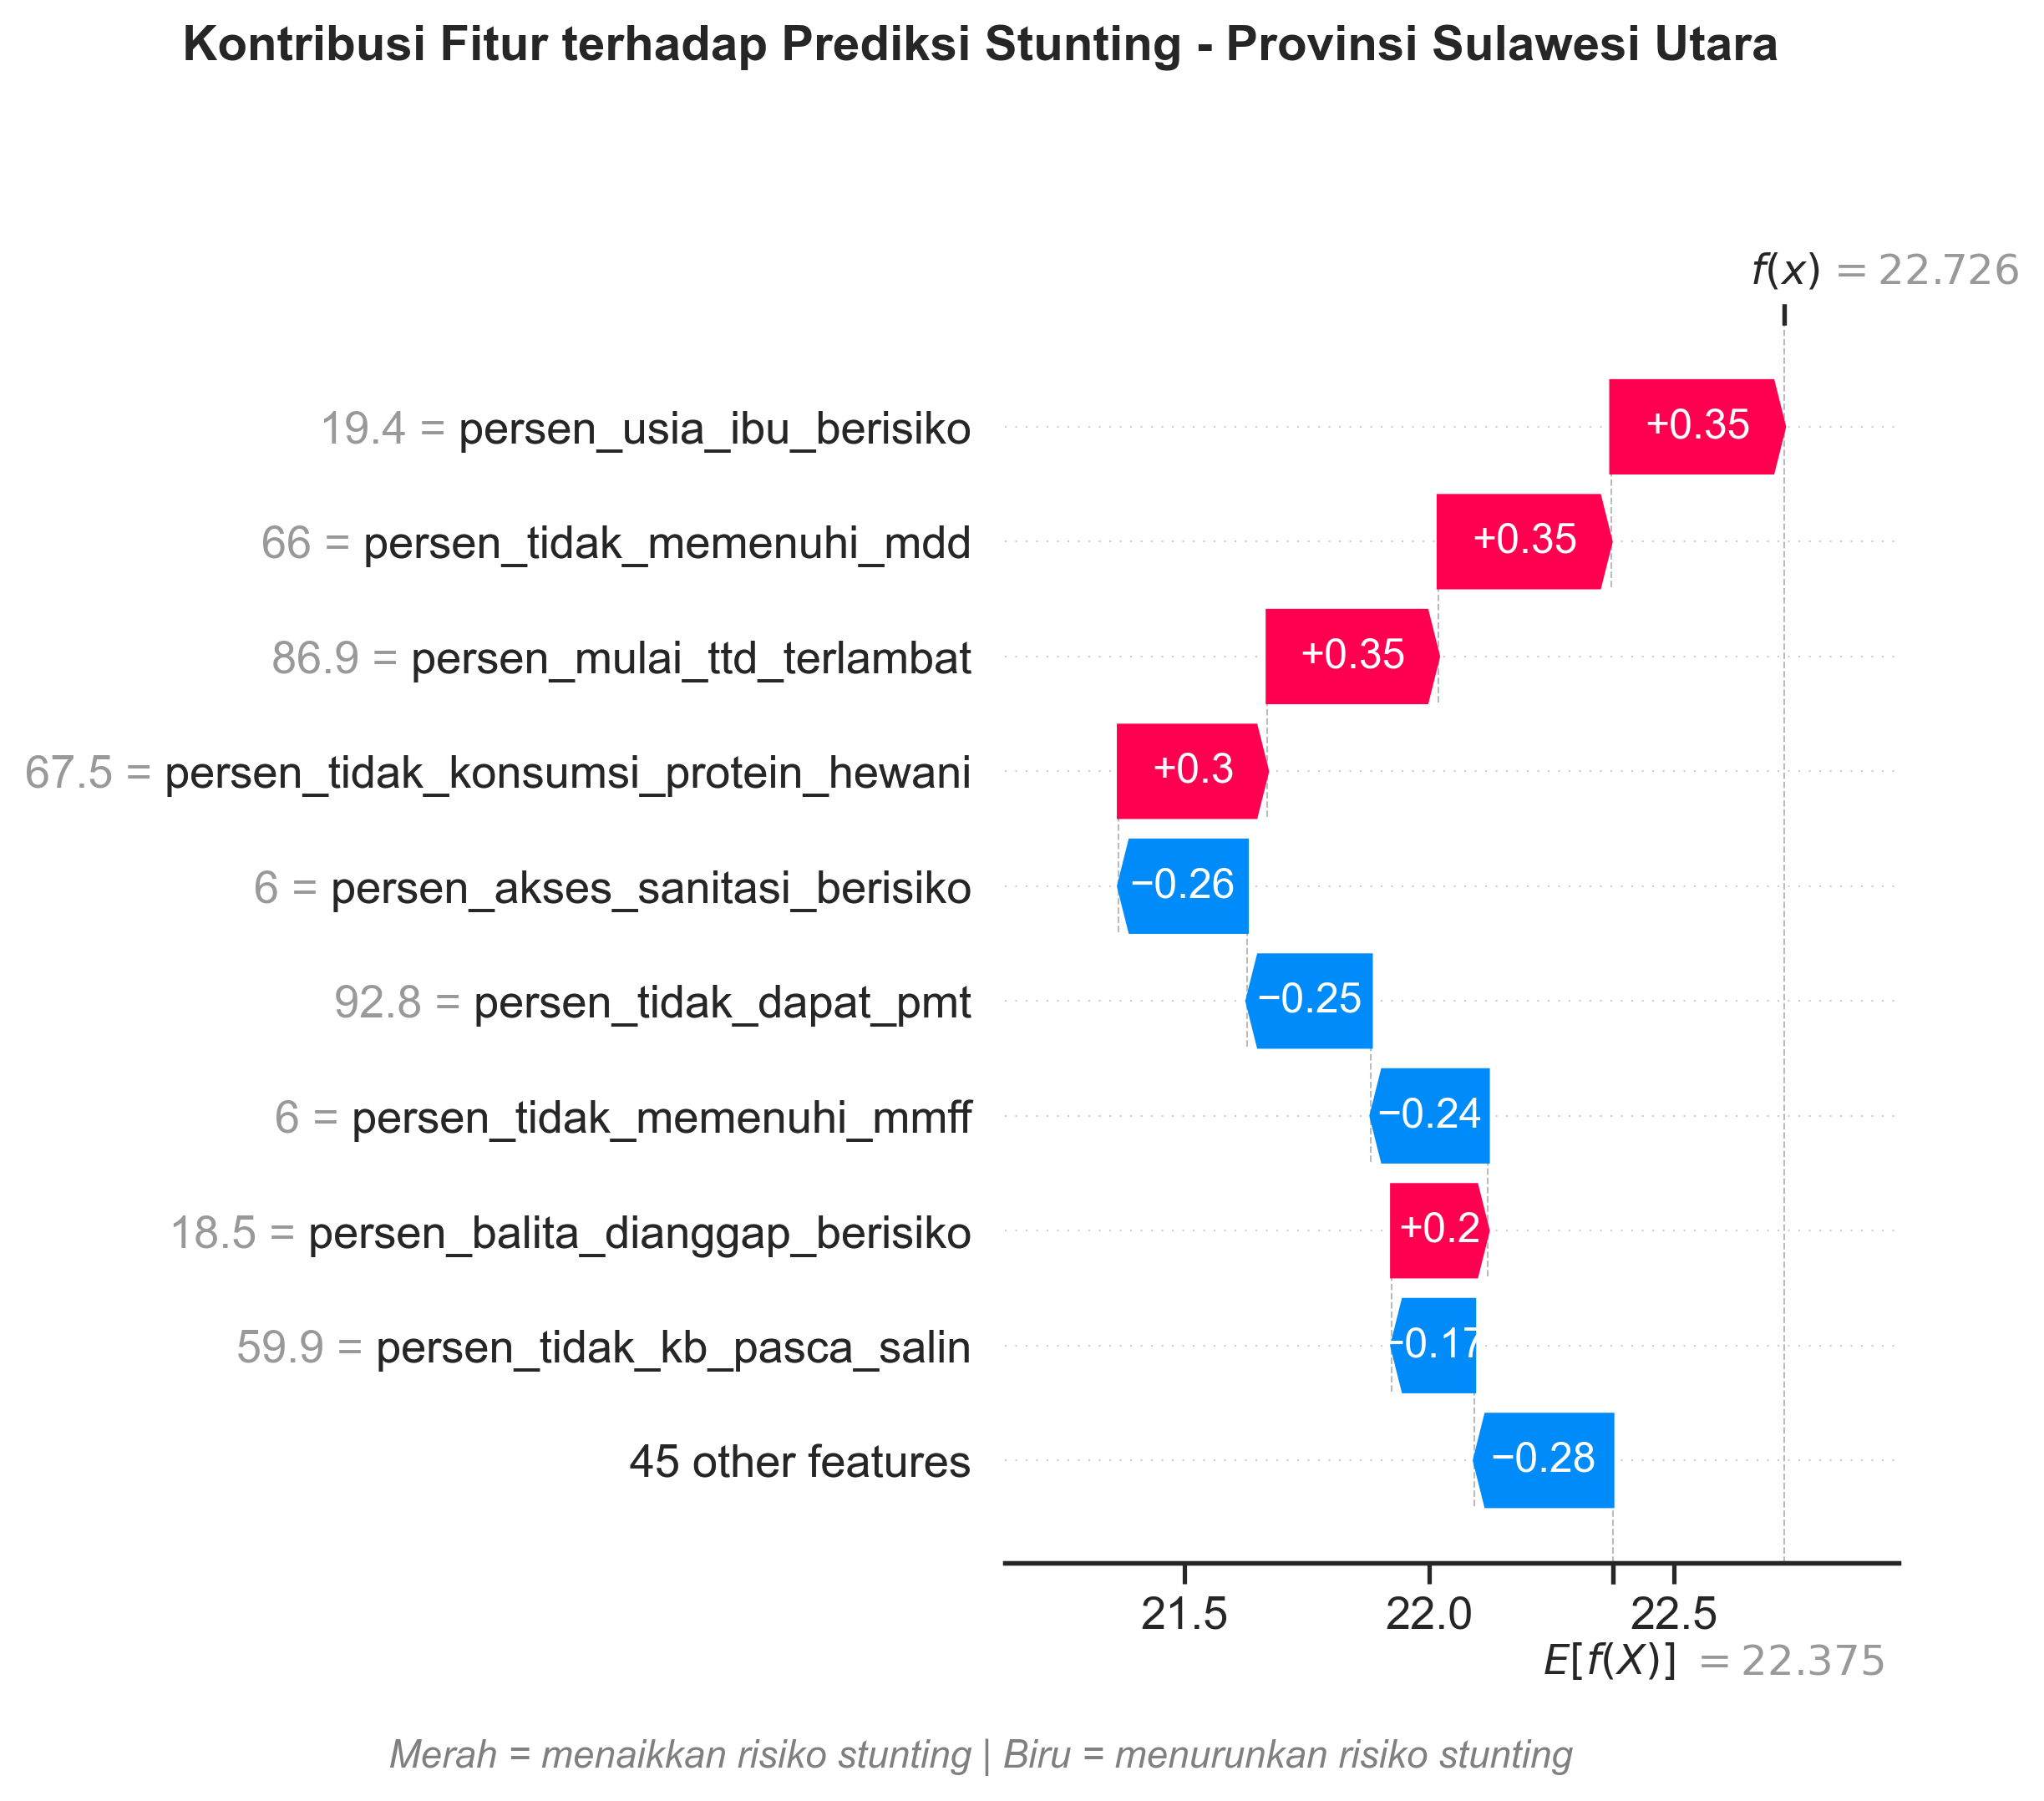
\includegraphics[width=0.48\textwidth]{figure/hasil_waterfall_stunting/waterfall_Sulawesi_Utara.png} \hfill
    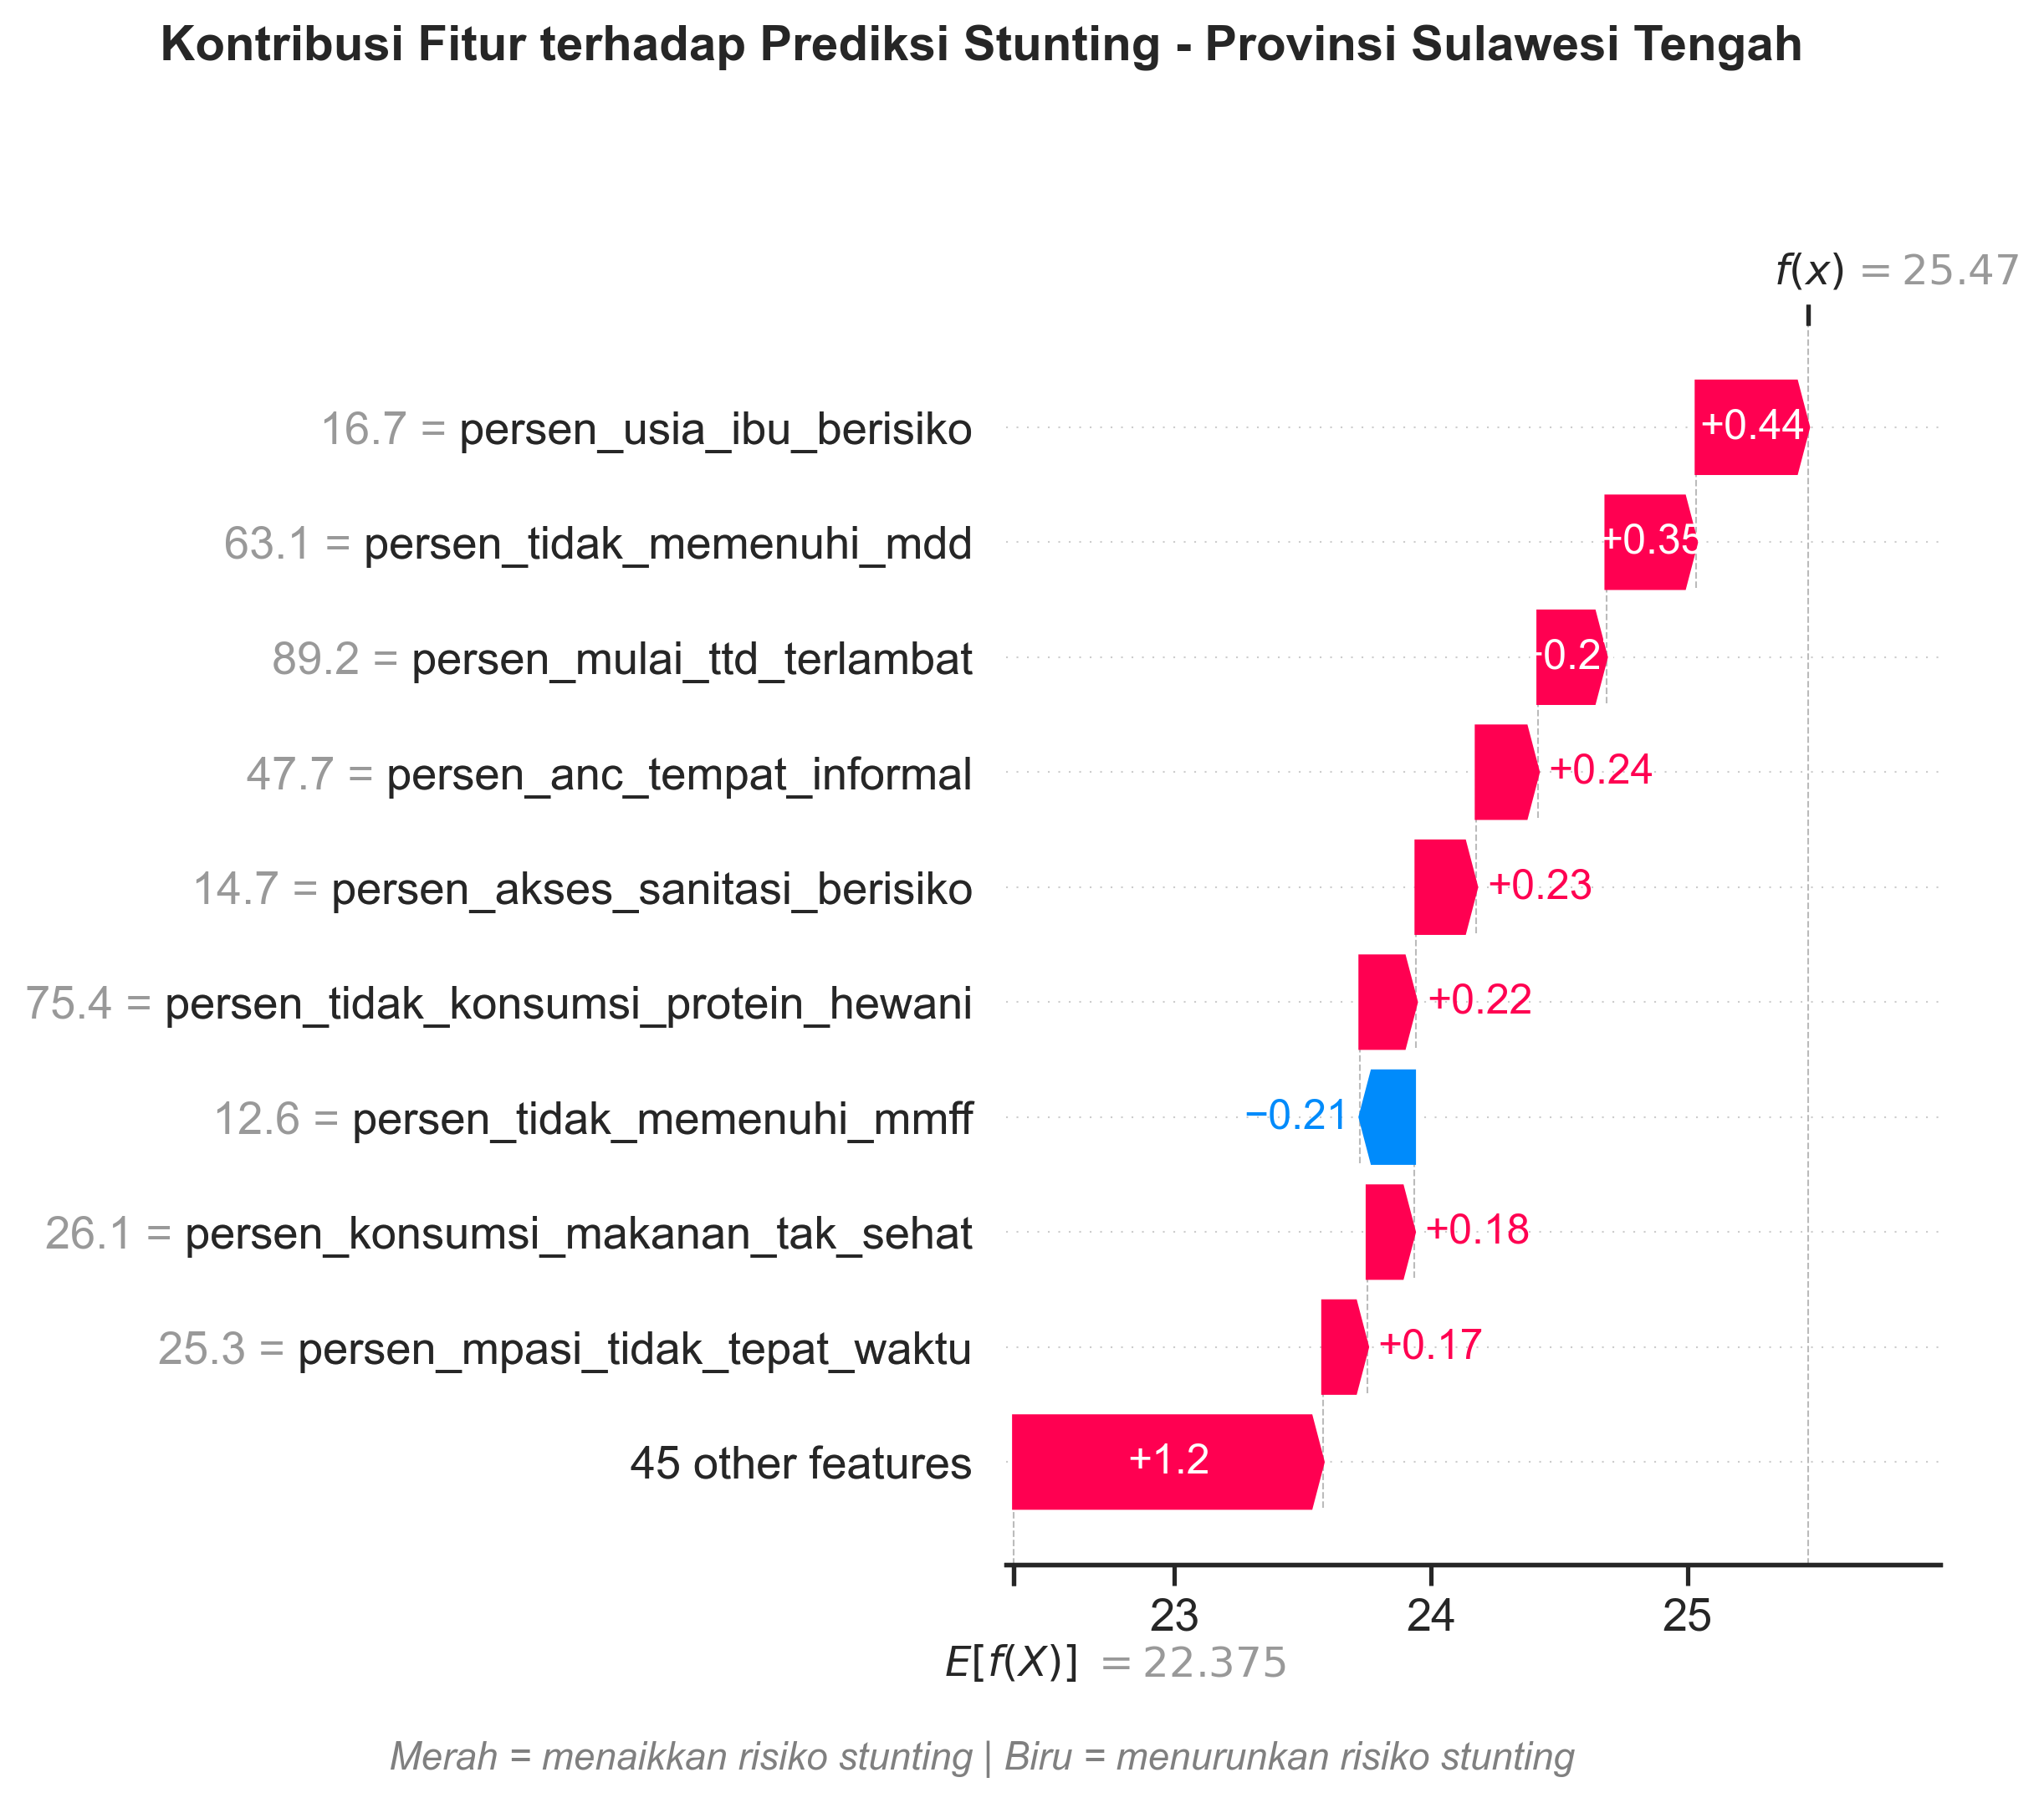
\includegraphics[width=0.48\textwidth]{figure/hasil_waterfall_stunting/waterfall_Sulawesi_Tengah.png} \\ \vspace{0.5cm}
    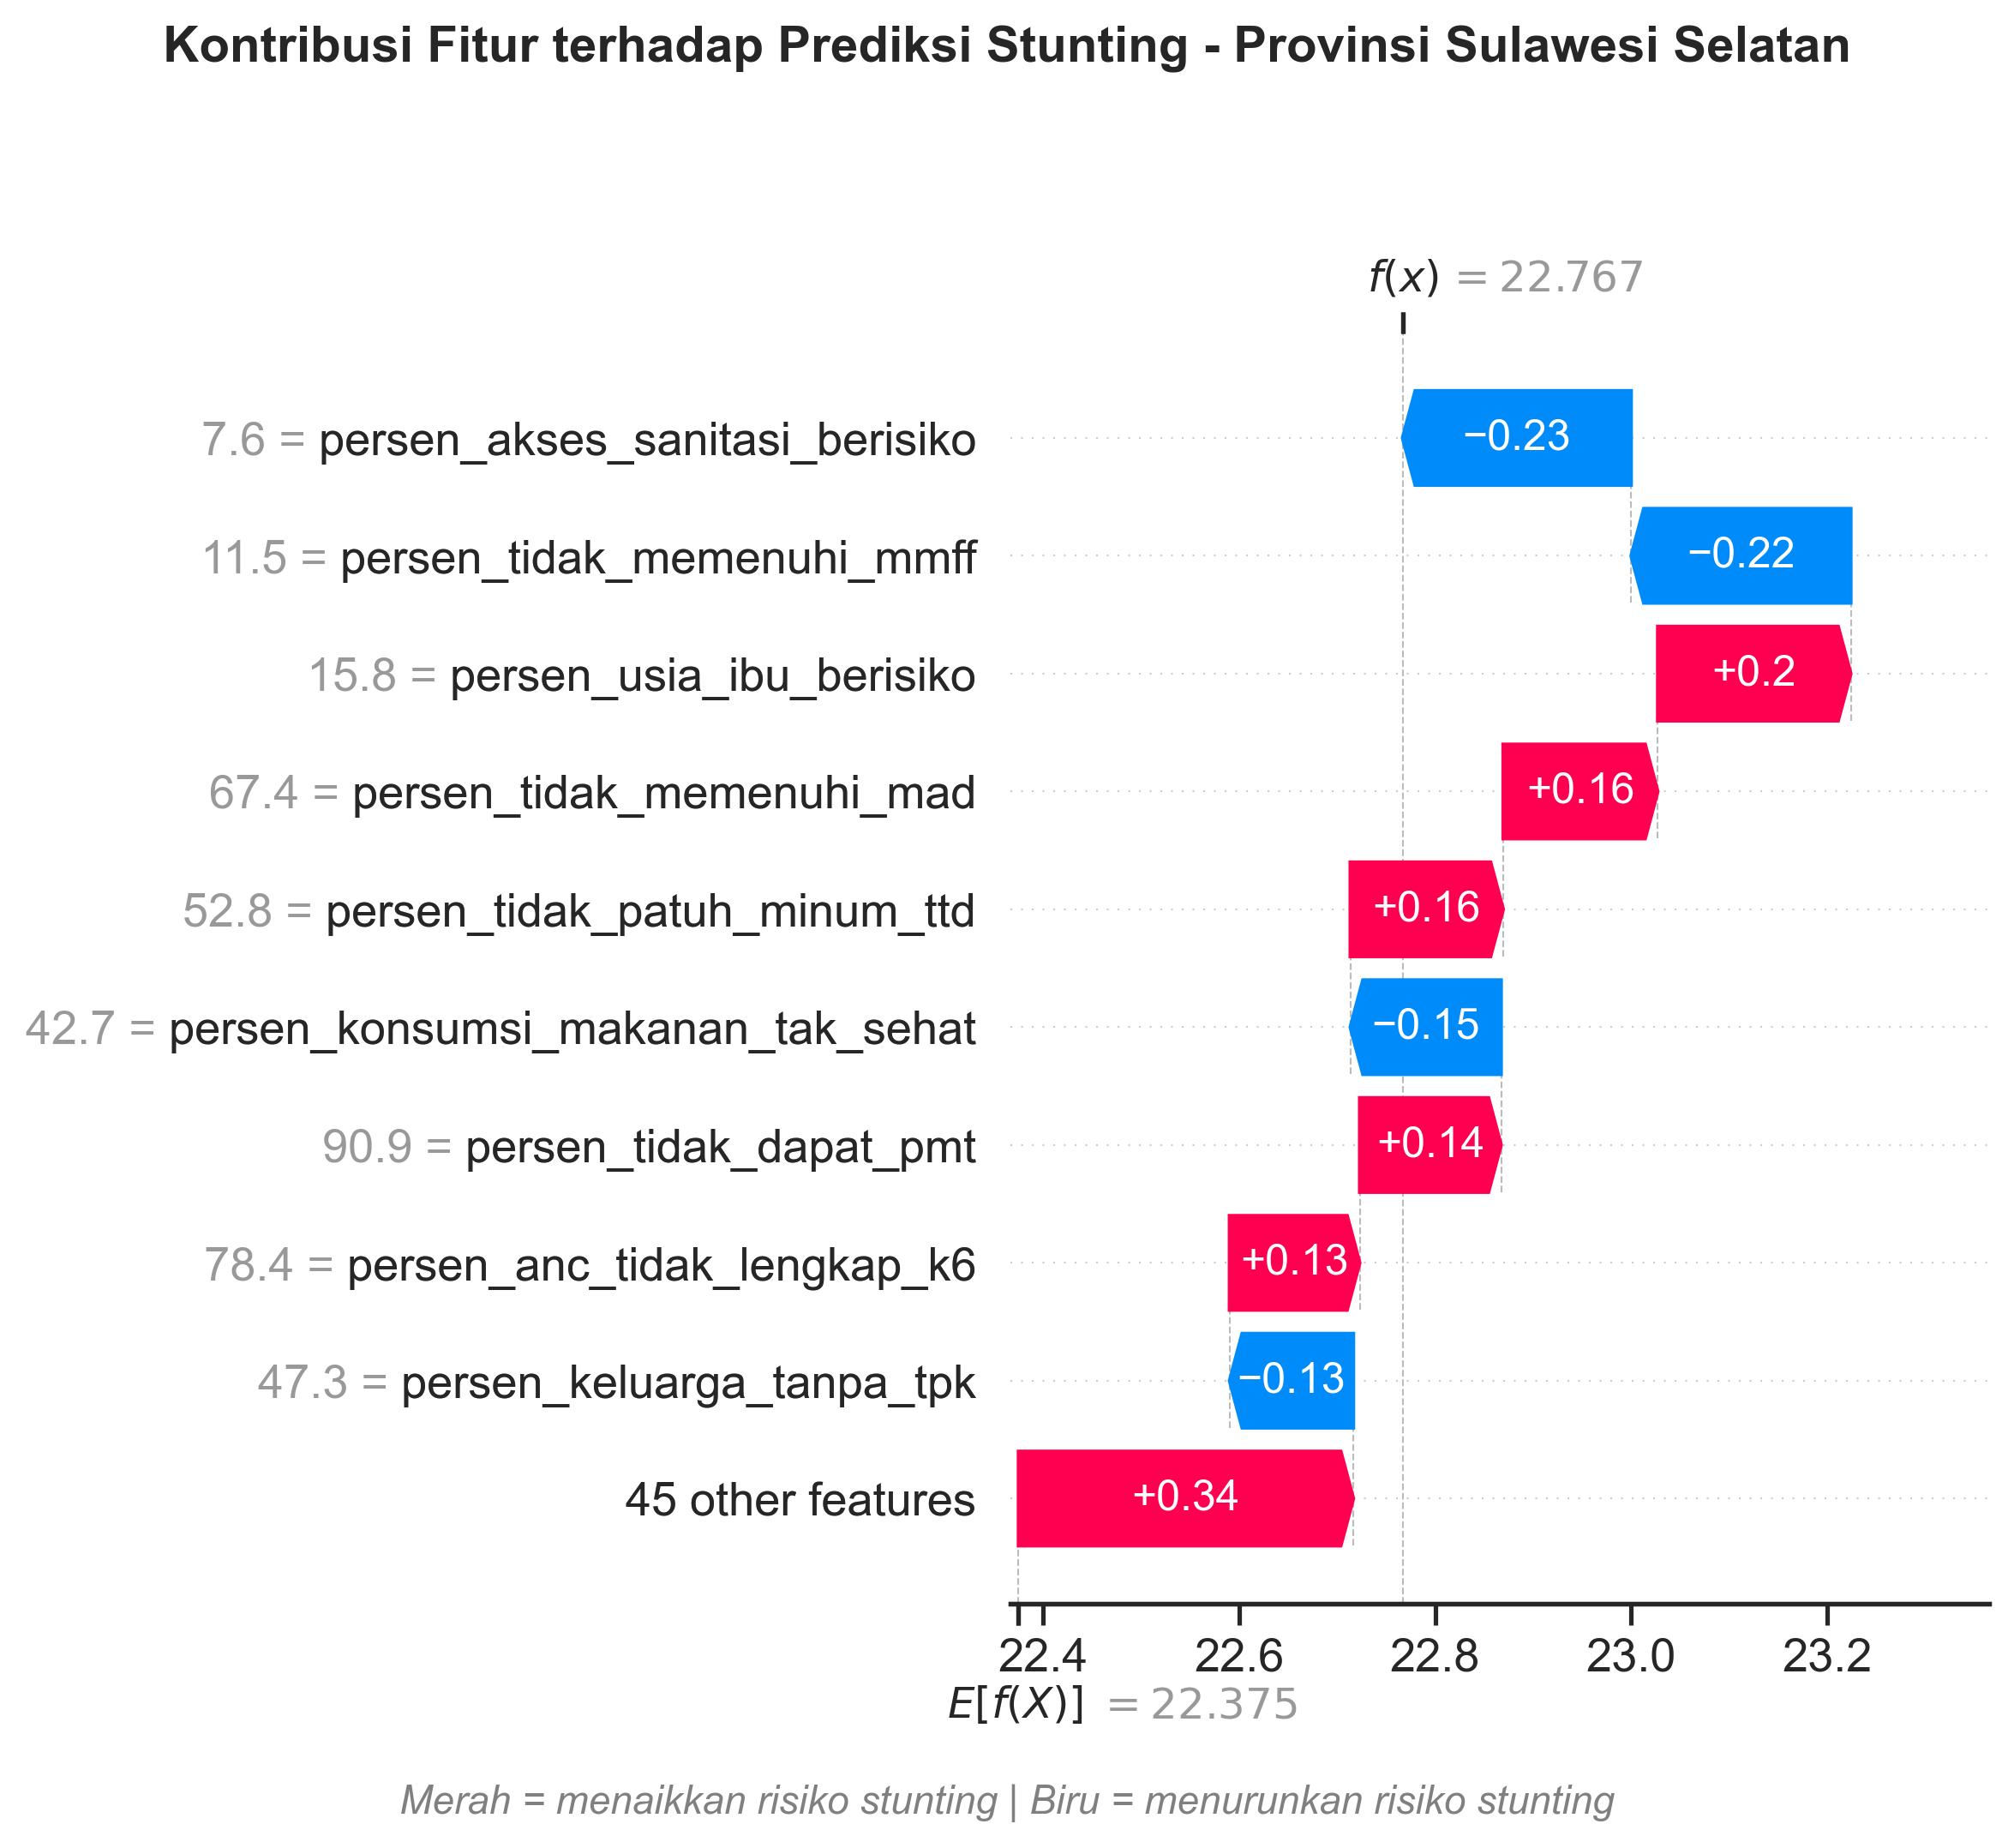
\includegraphics[width=0.48\textwidth]{figure/hasil_waterfall_stunting/waterfall_Sulawesi_Selatan.png} \hfill
    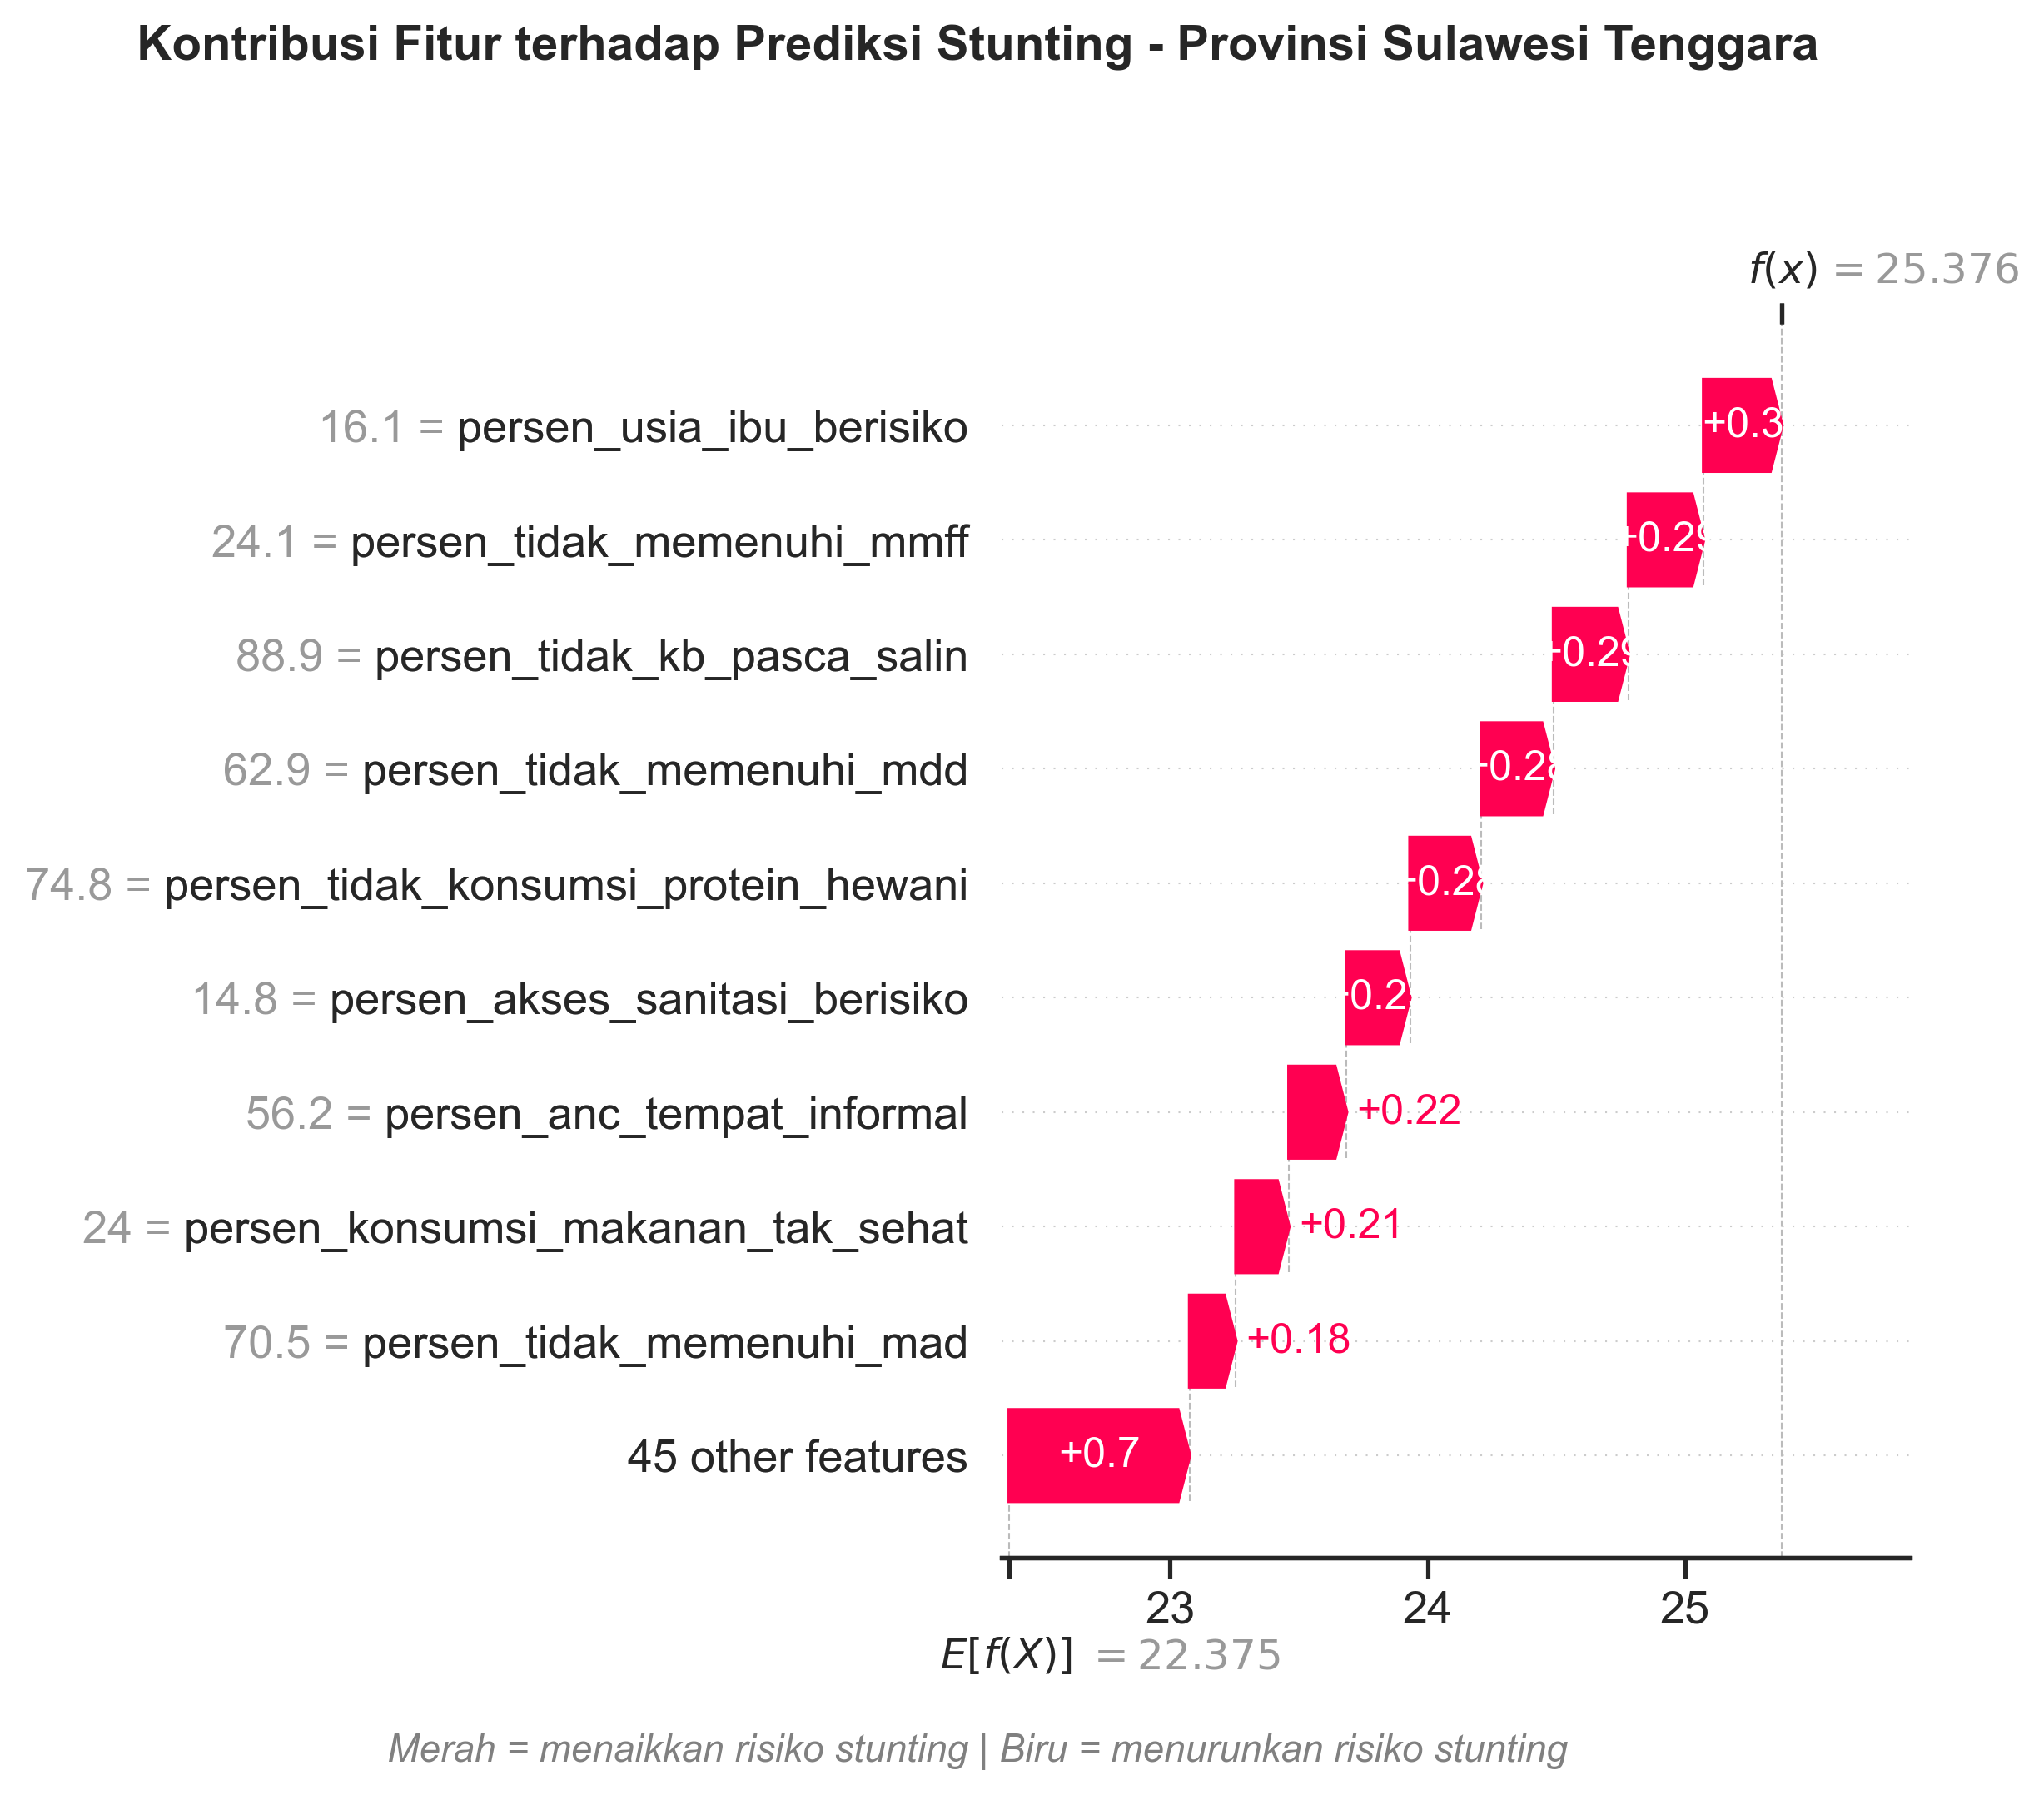
\includegraphics[width=0.48\textwidth]{figure/hasil_waterfall_stunting/waterfall_Sulawesi_Tenggara.png} \\ \vspace{0.5cm}
    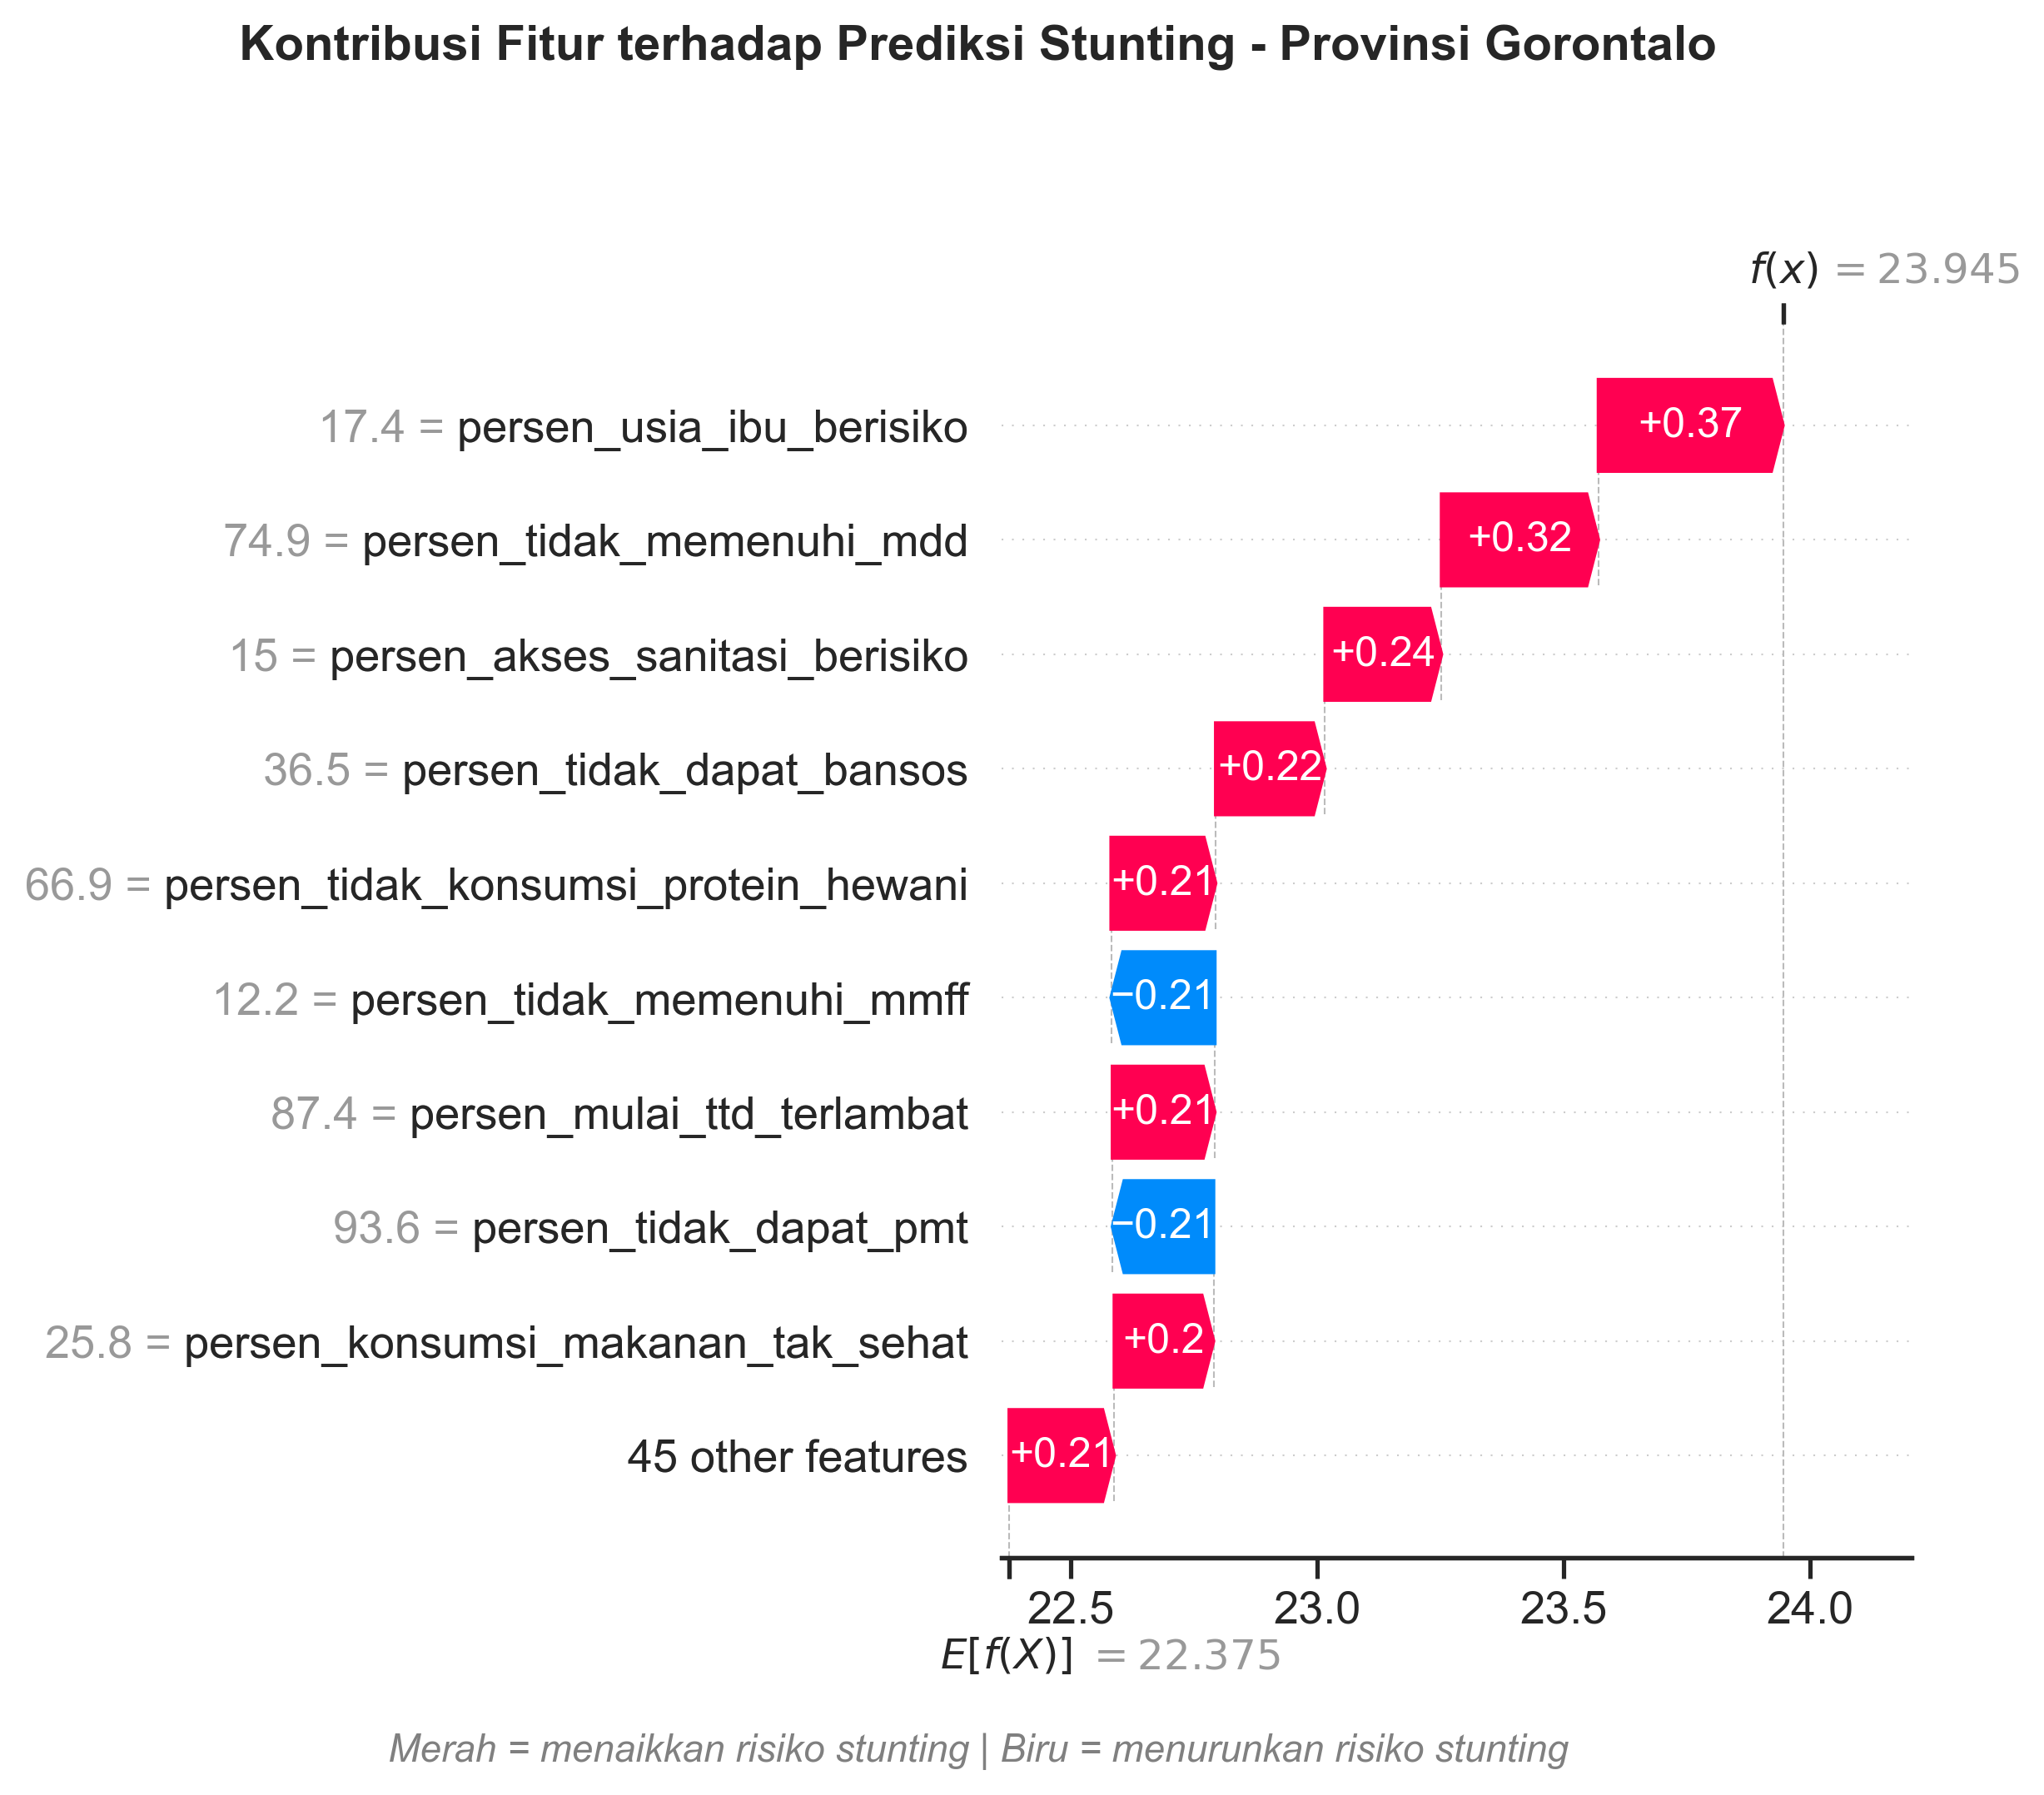
\includegraphics[width=0.48\textwidth]{figure/hasil_waterfall_stunting/waterfall_Gorontalo.png} \hfill
    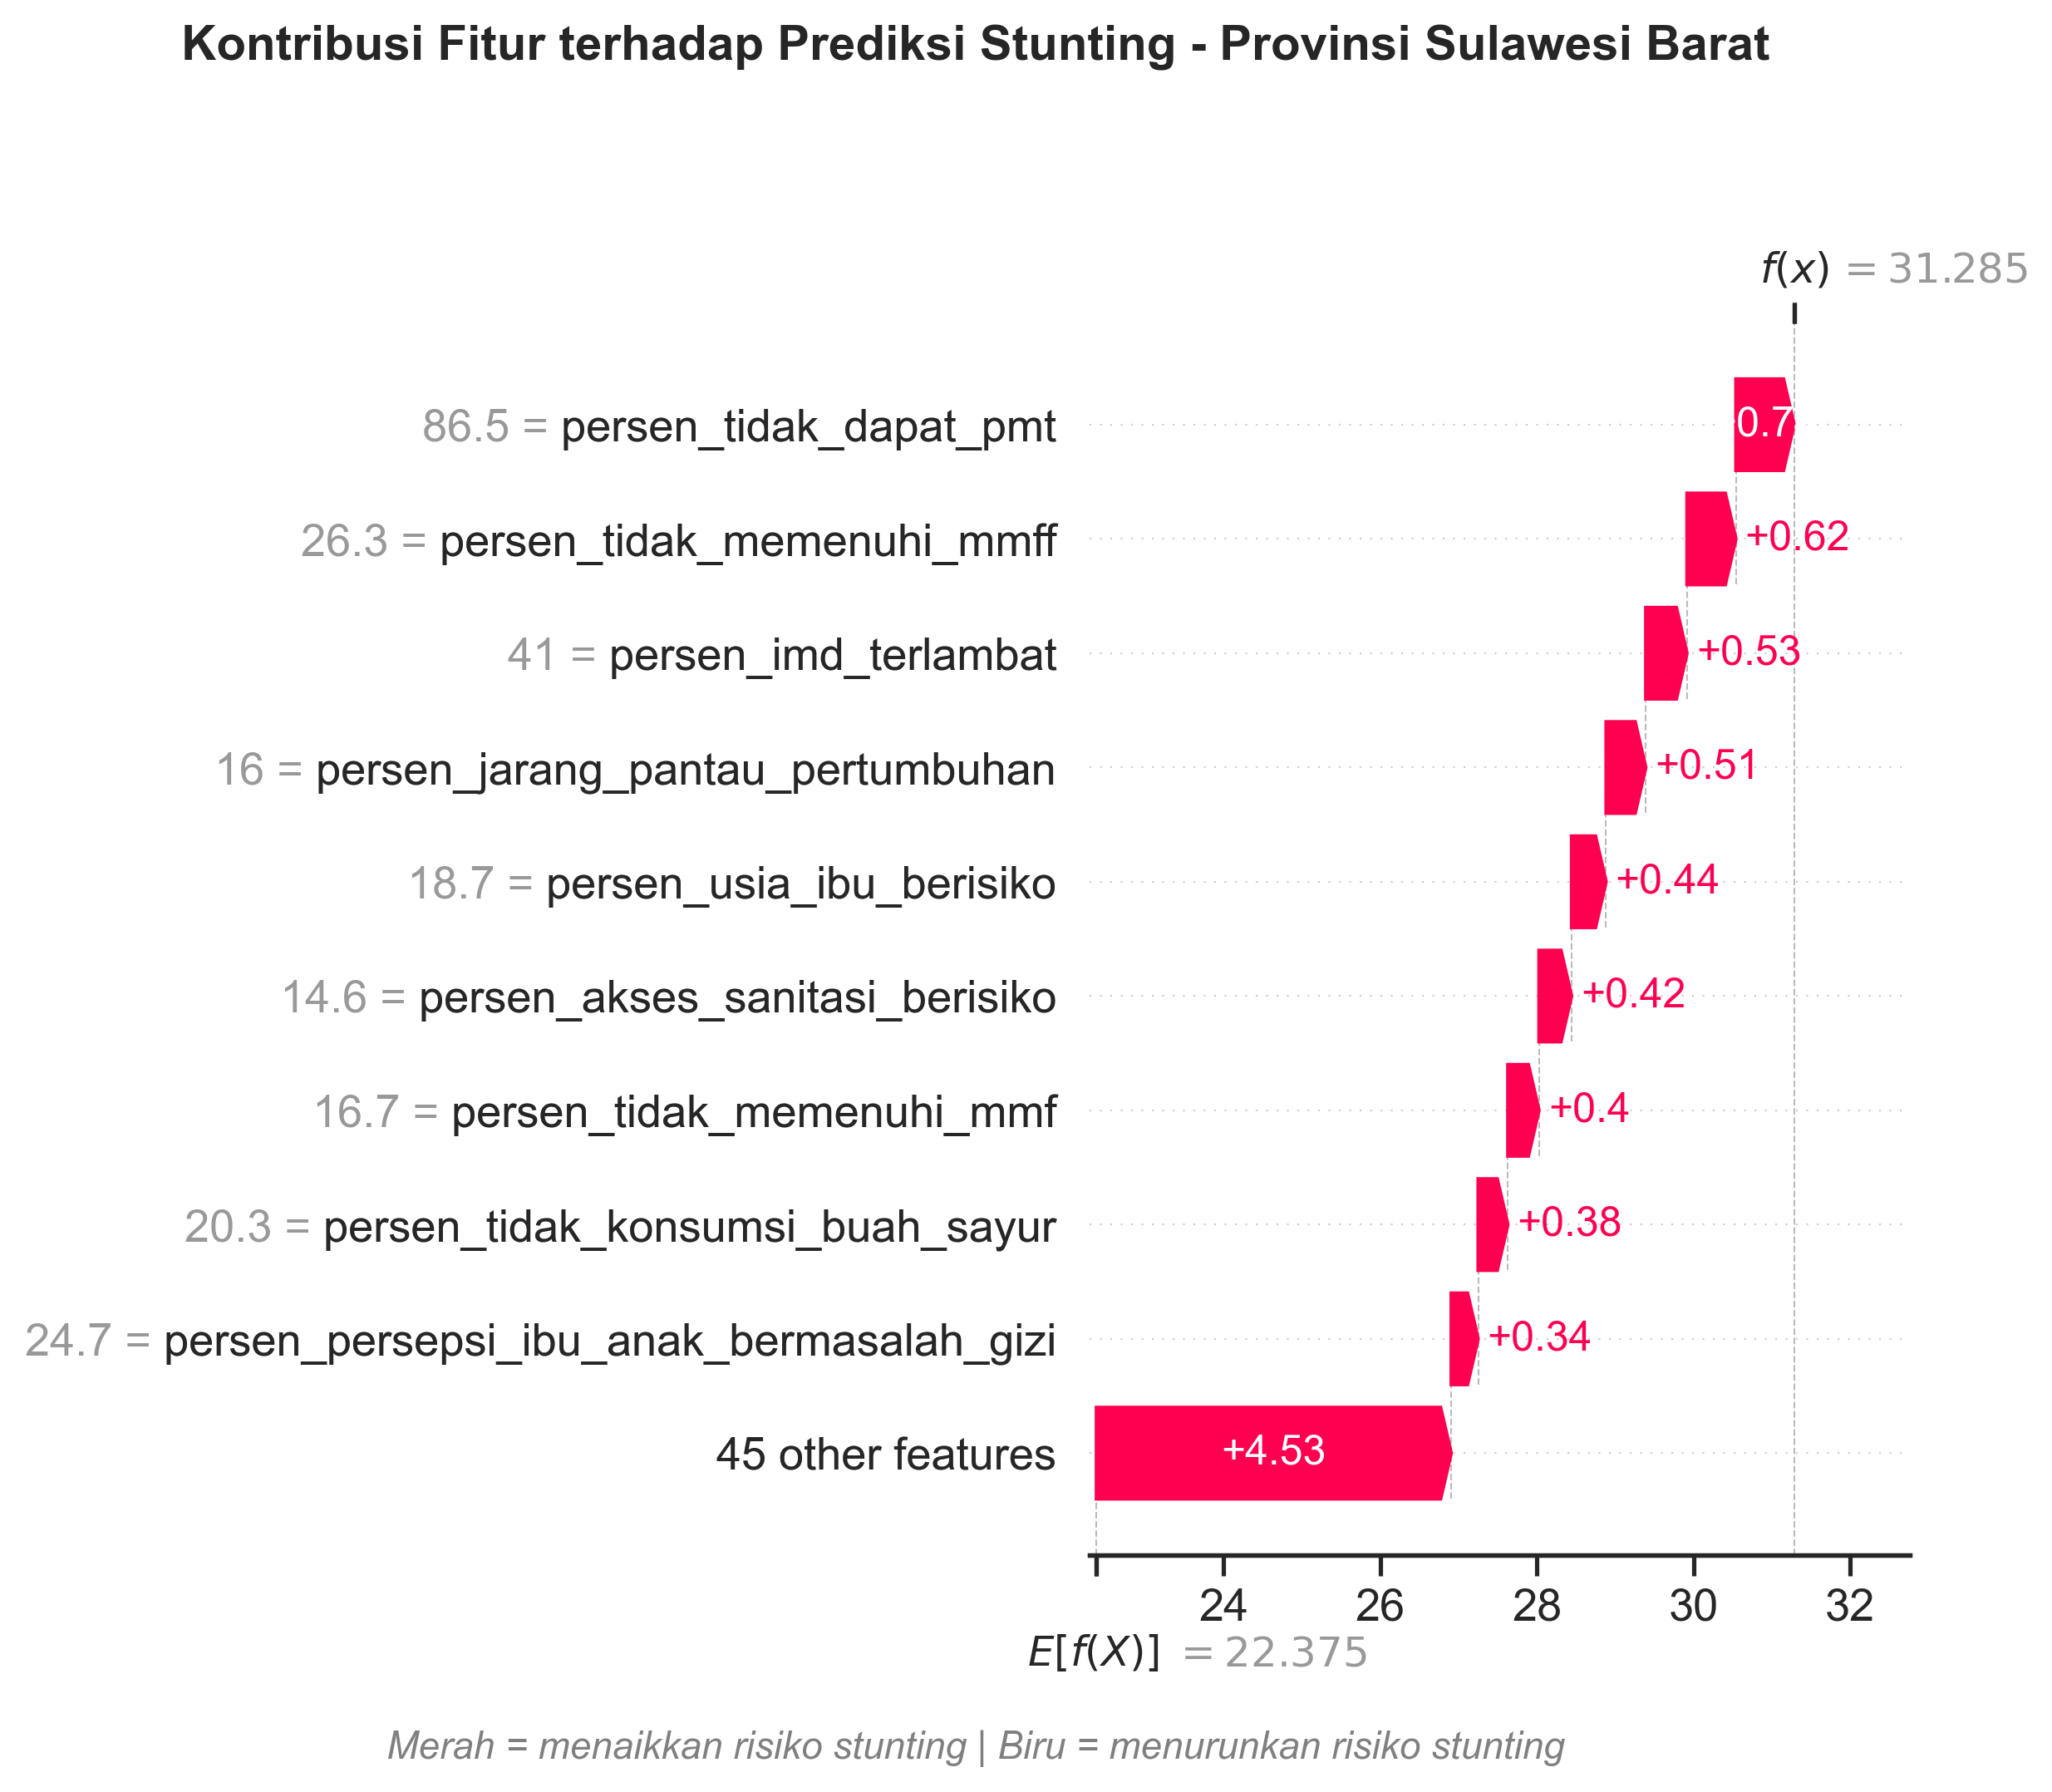
\includegraphics[width=0.48\textwidth]{figure/hasil_waterfall_stunting/waterfall_Sulawesi_Barat.png}
\end{figure}

\newpage
\begin{figure}[H]
    \centering
    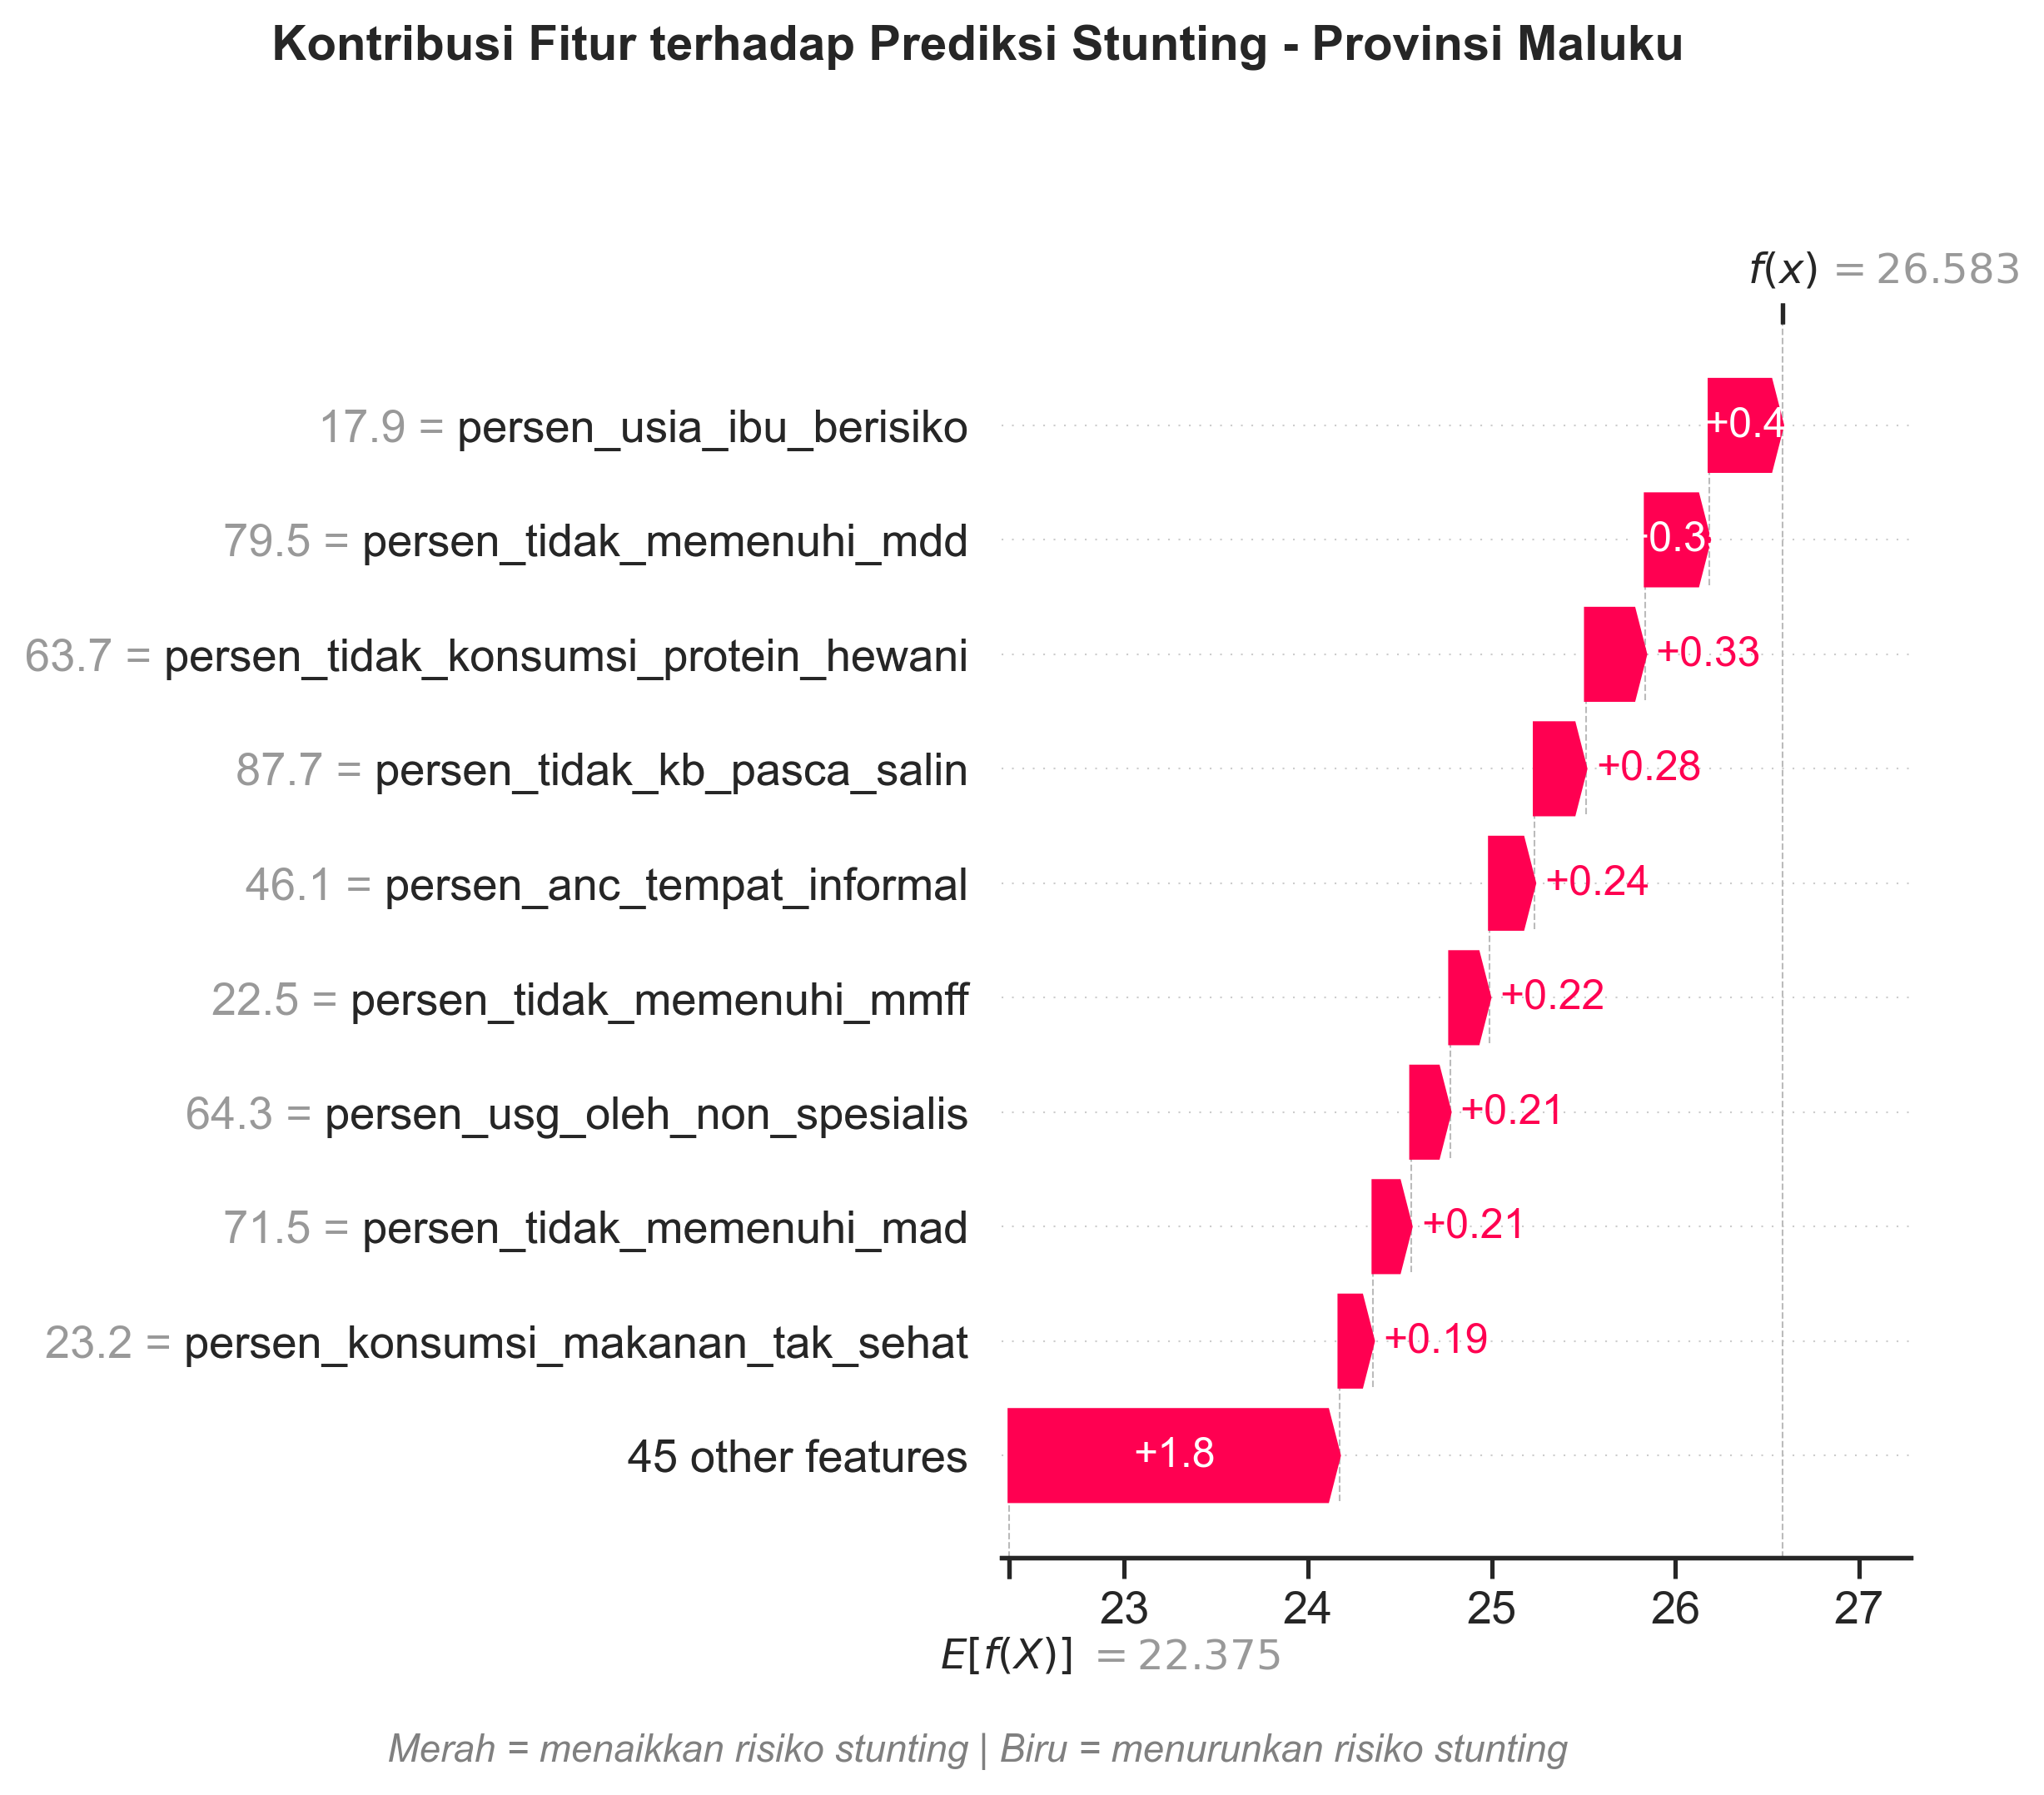
\includegraphics[width=0.48\textwidth]{figure/hasil_waterfall_stunting/waterfall_Maluku.png} \hfill
    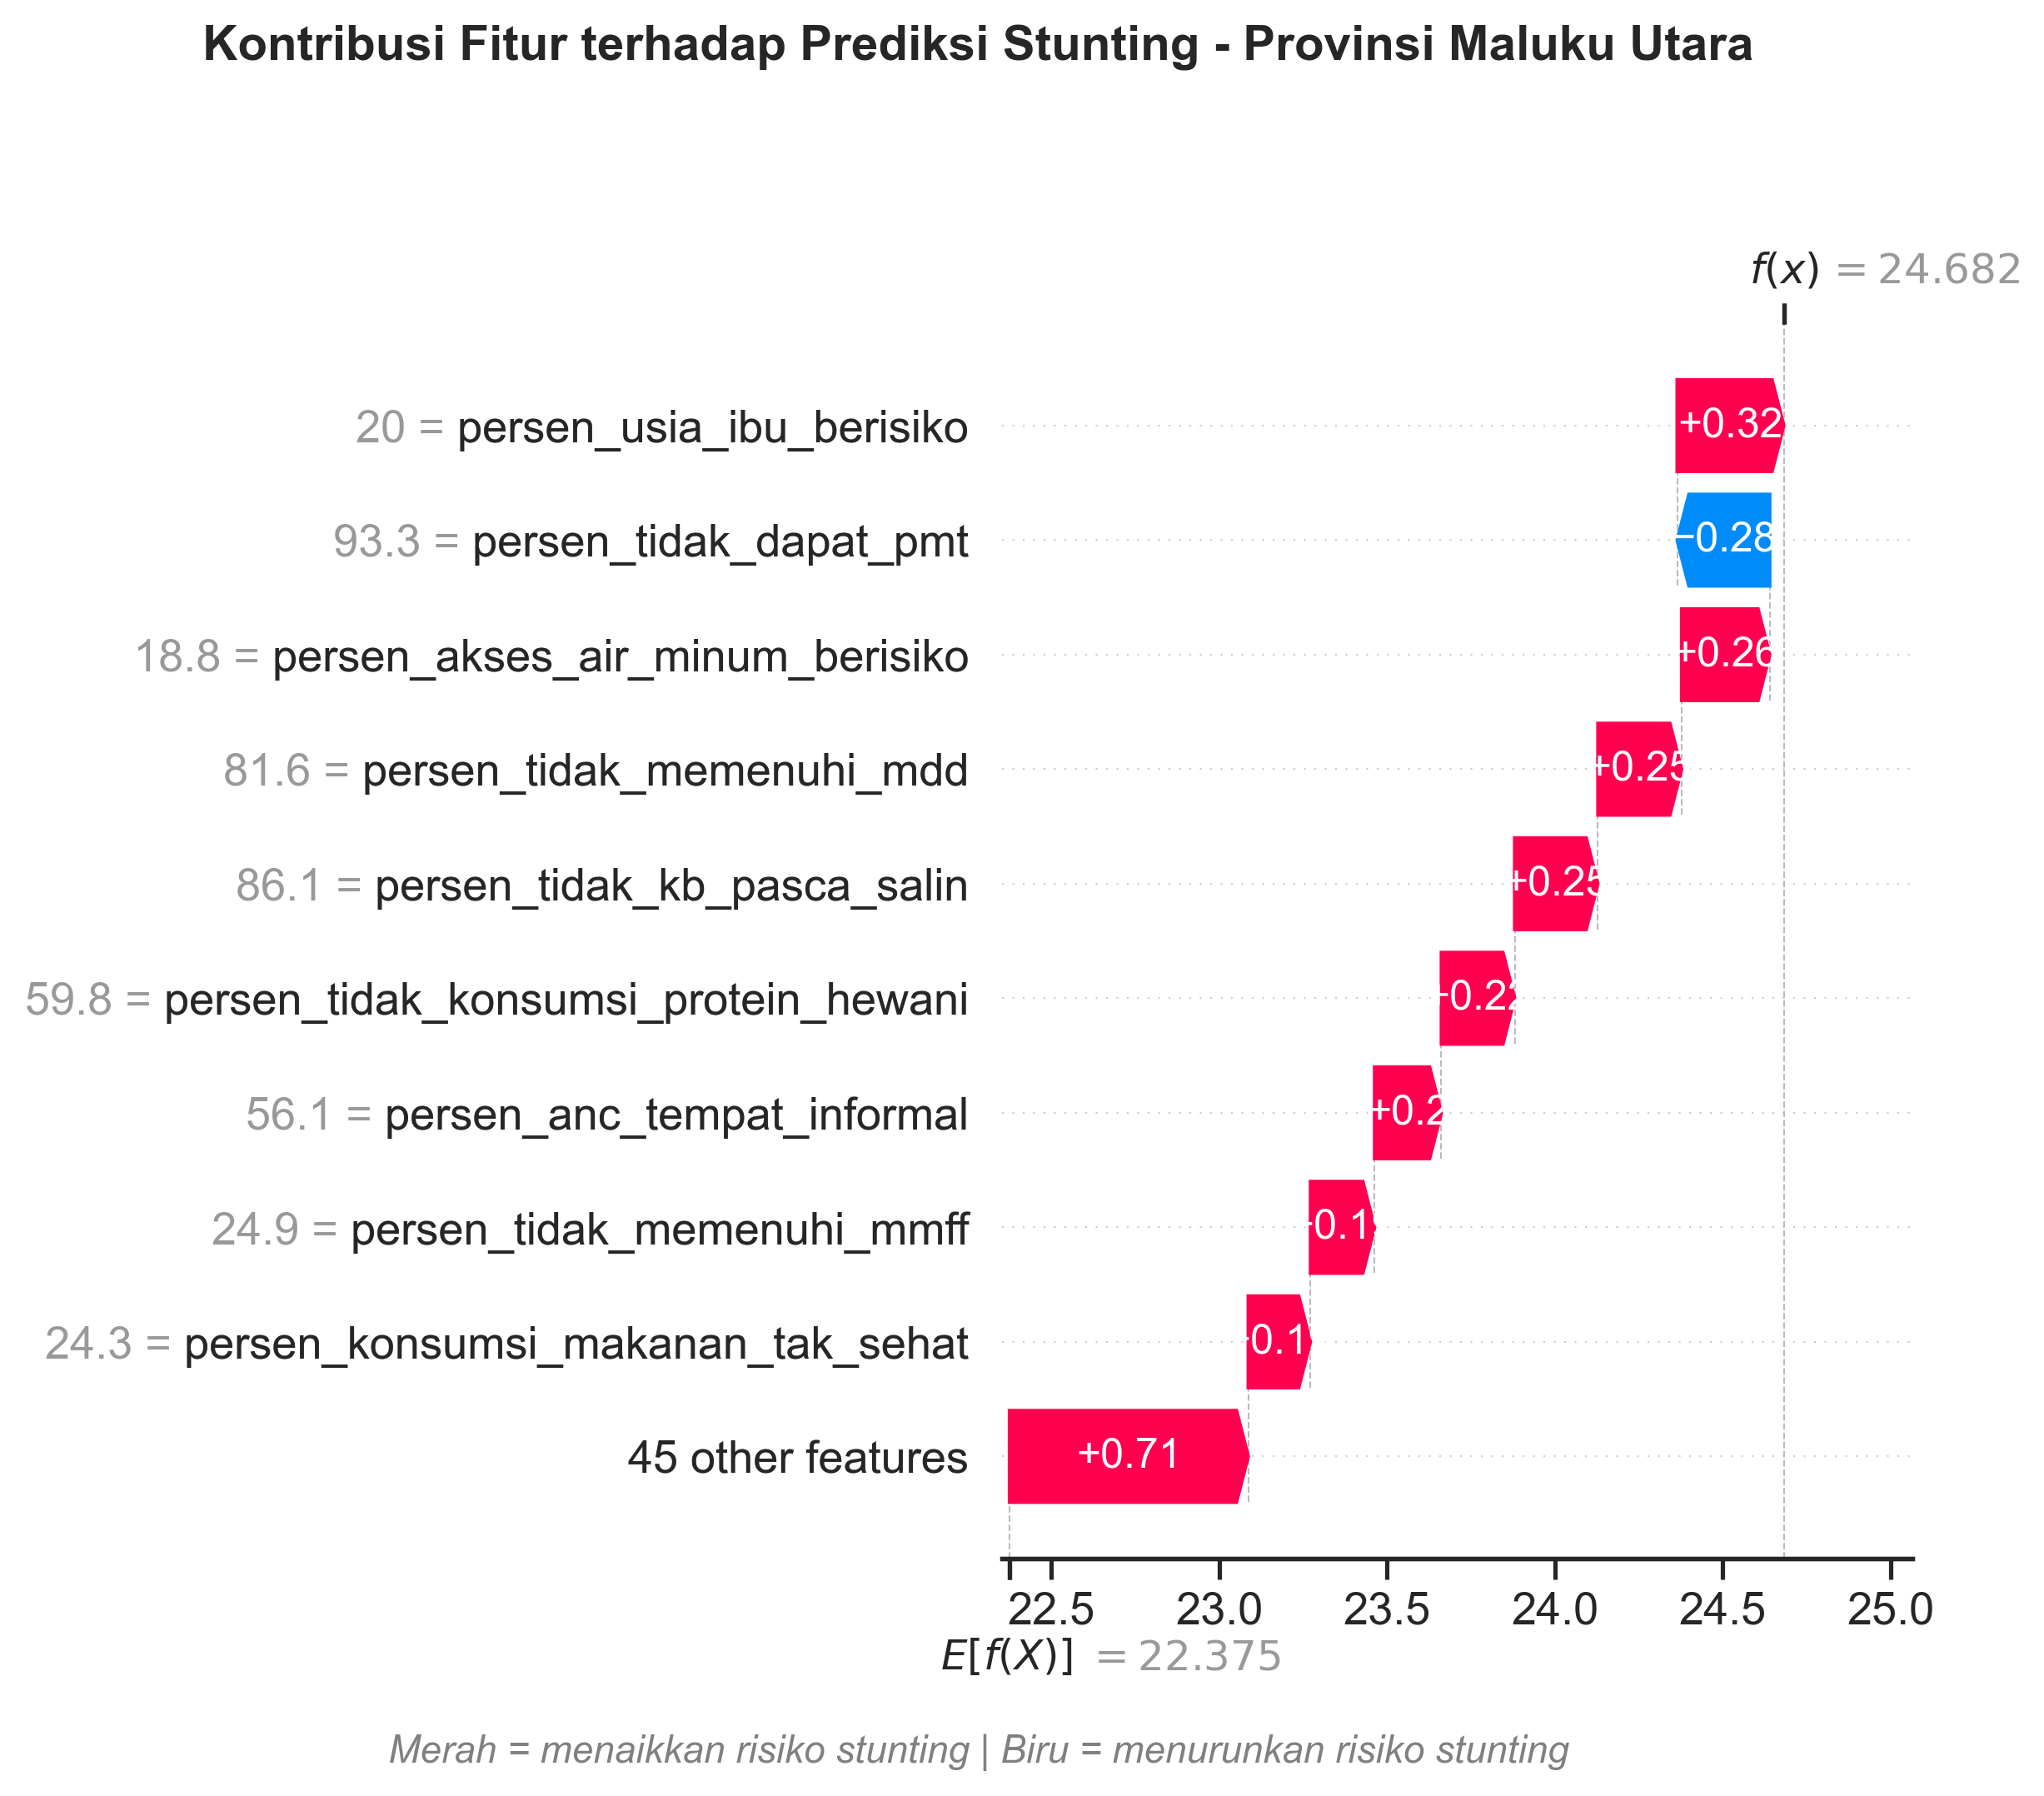
\includegraphics[width=0.48\textwidth]{figure/hasil_waterfall_stunting/waterfall_Maluku_Utara.png} \\ \vspace{0.5cm}
    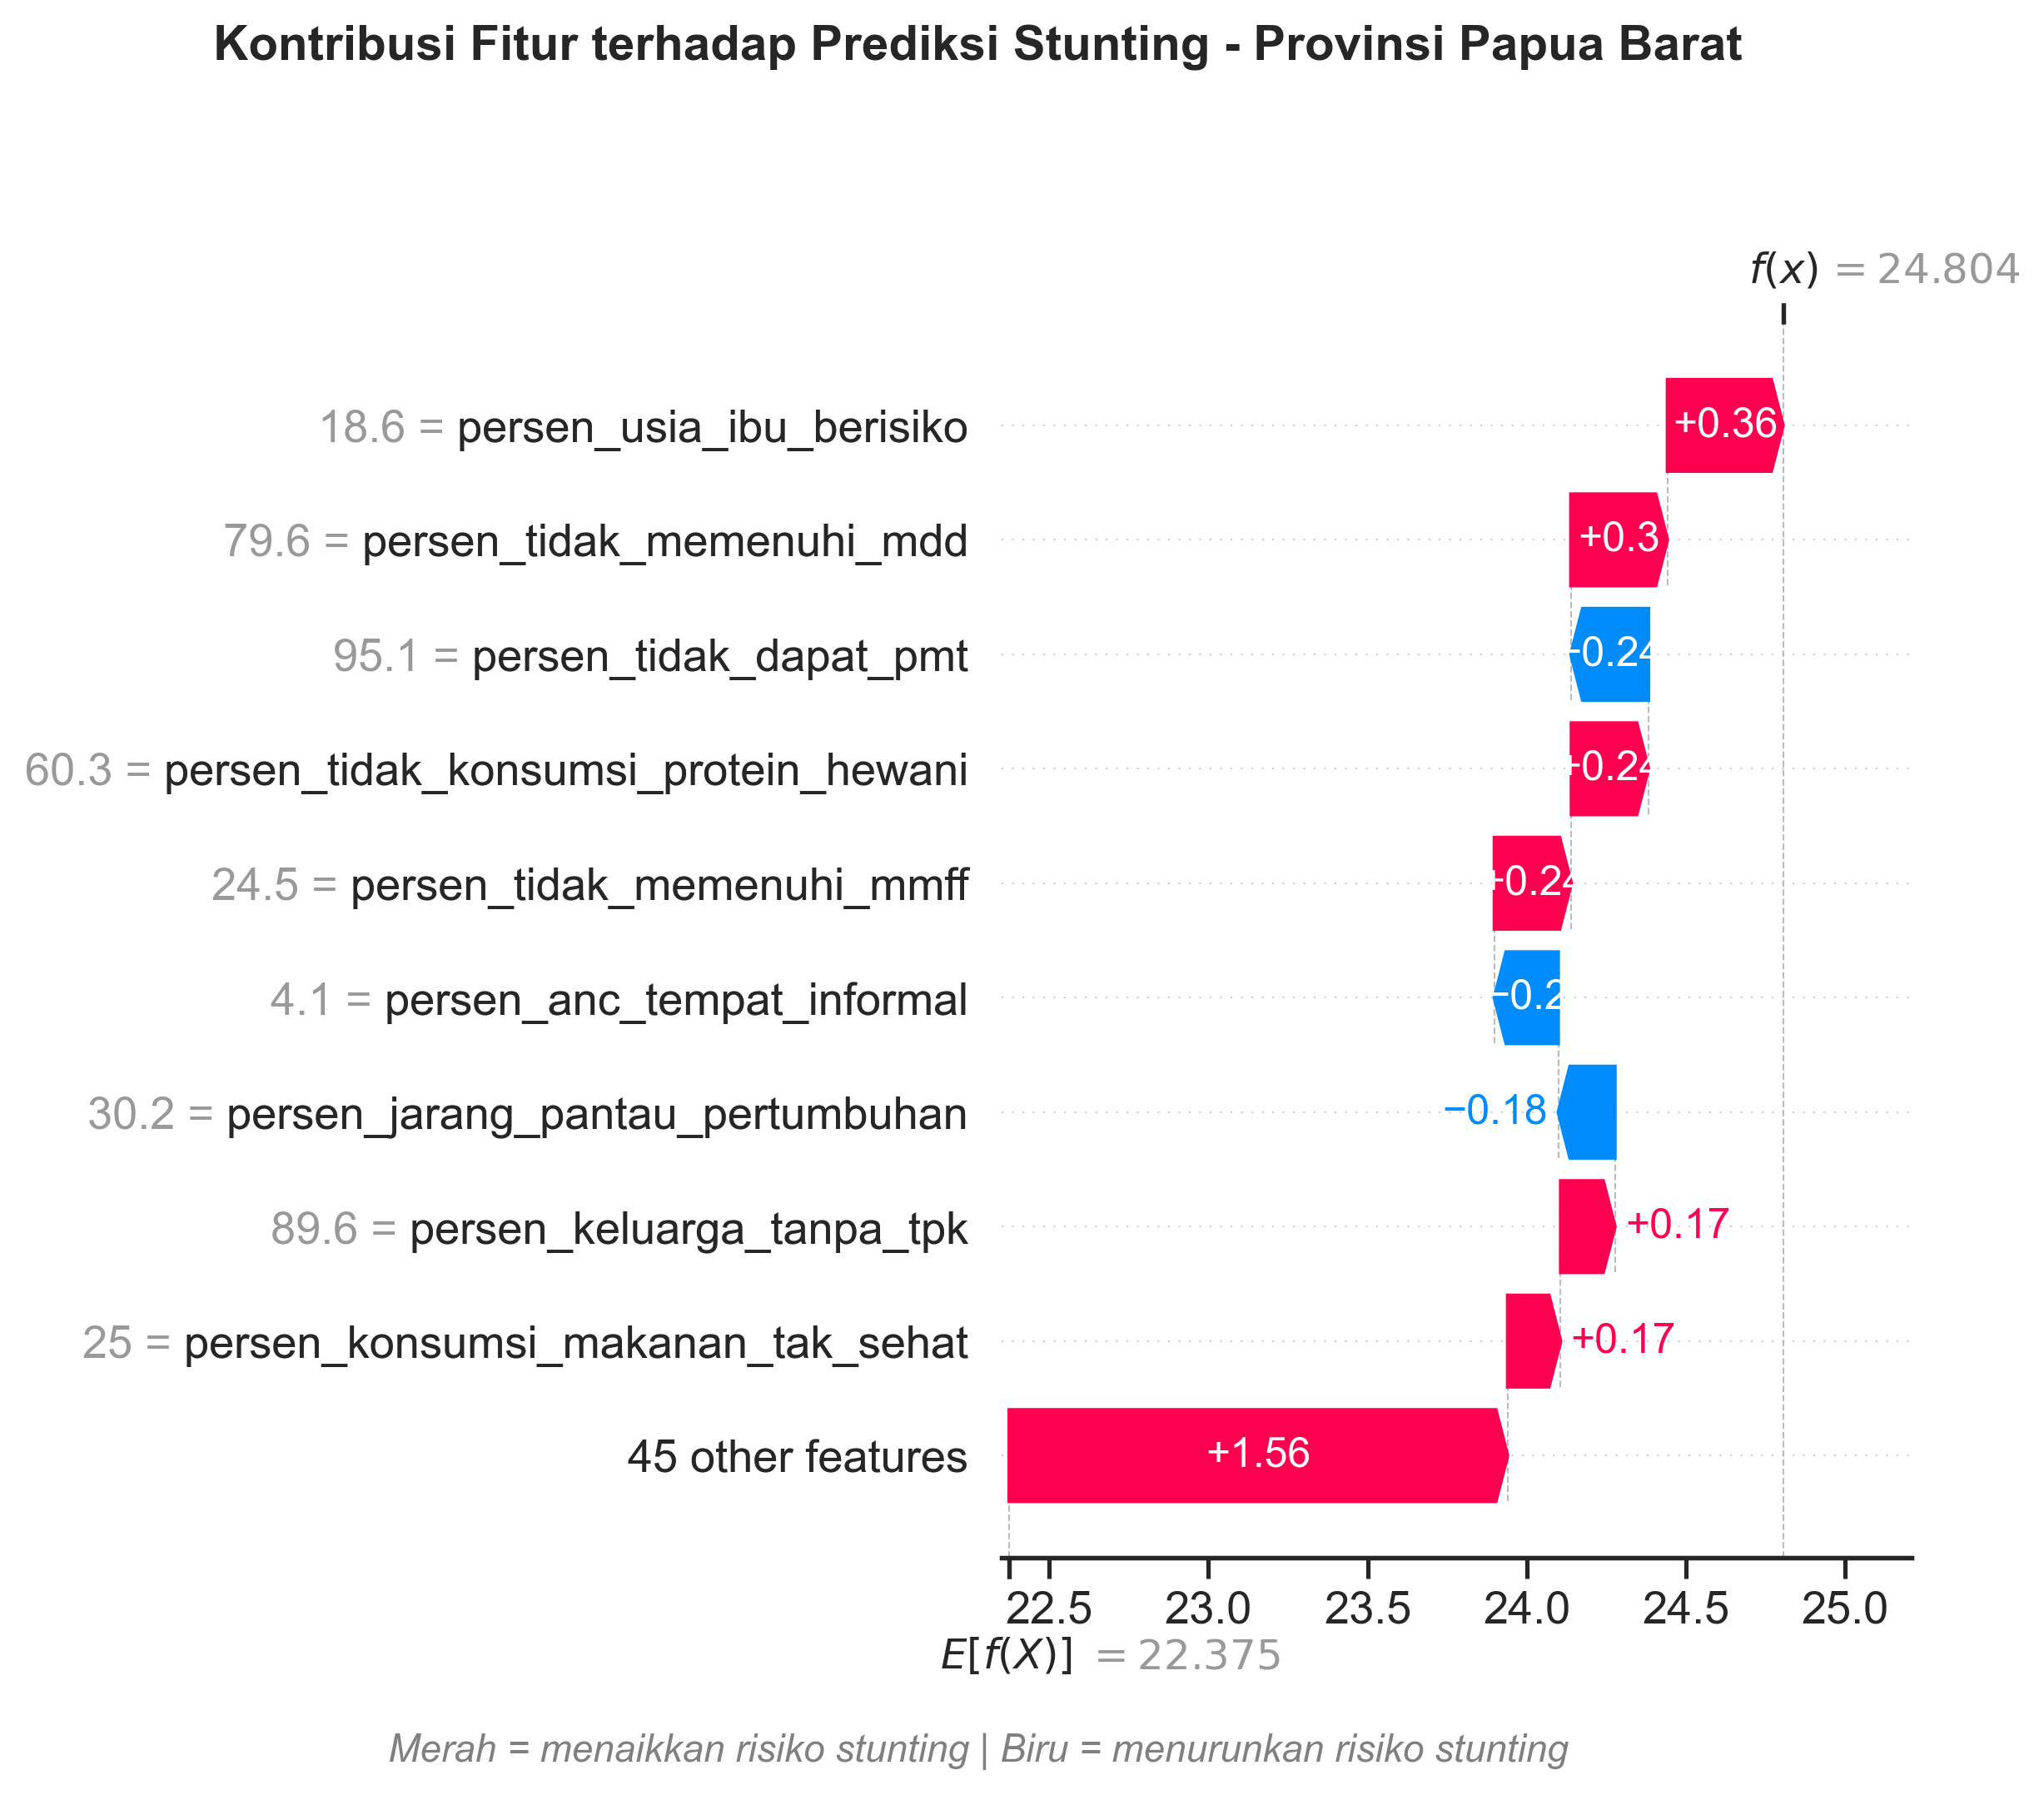
\includegraphics[width=0.48\textwidth]{figure/hasil_waterfall_stunting/waterfall_Papua_Barat.png} \hfill
    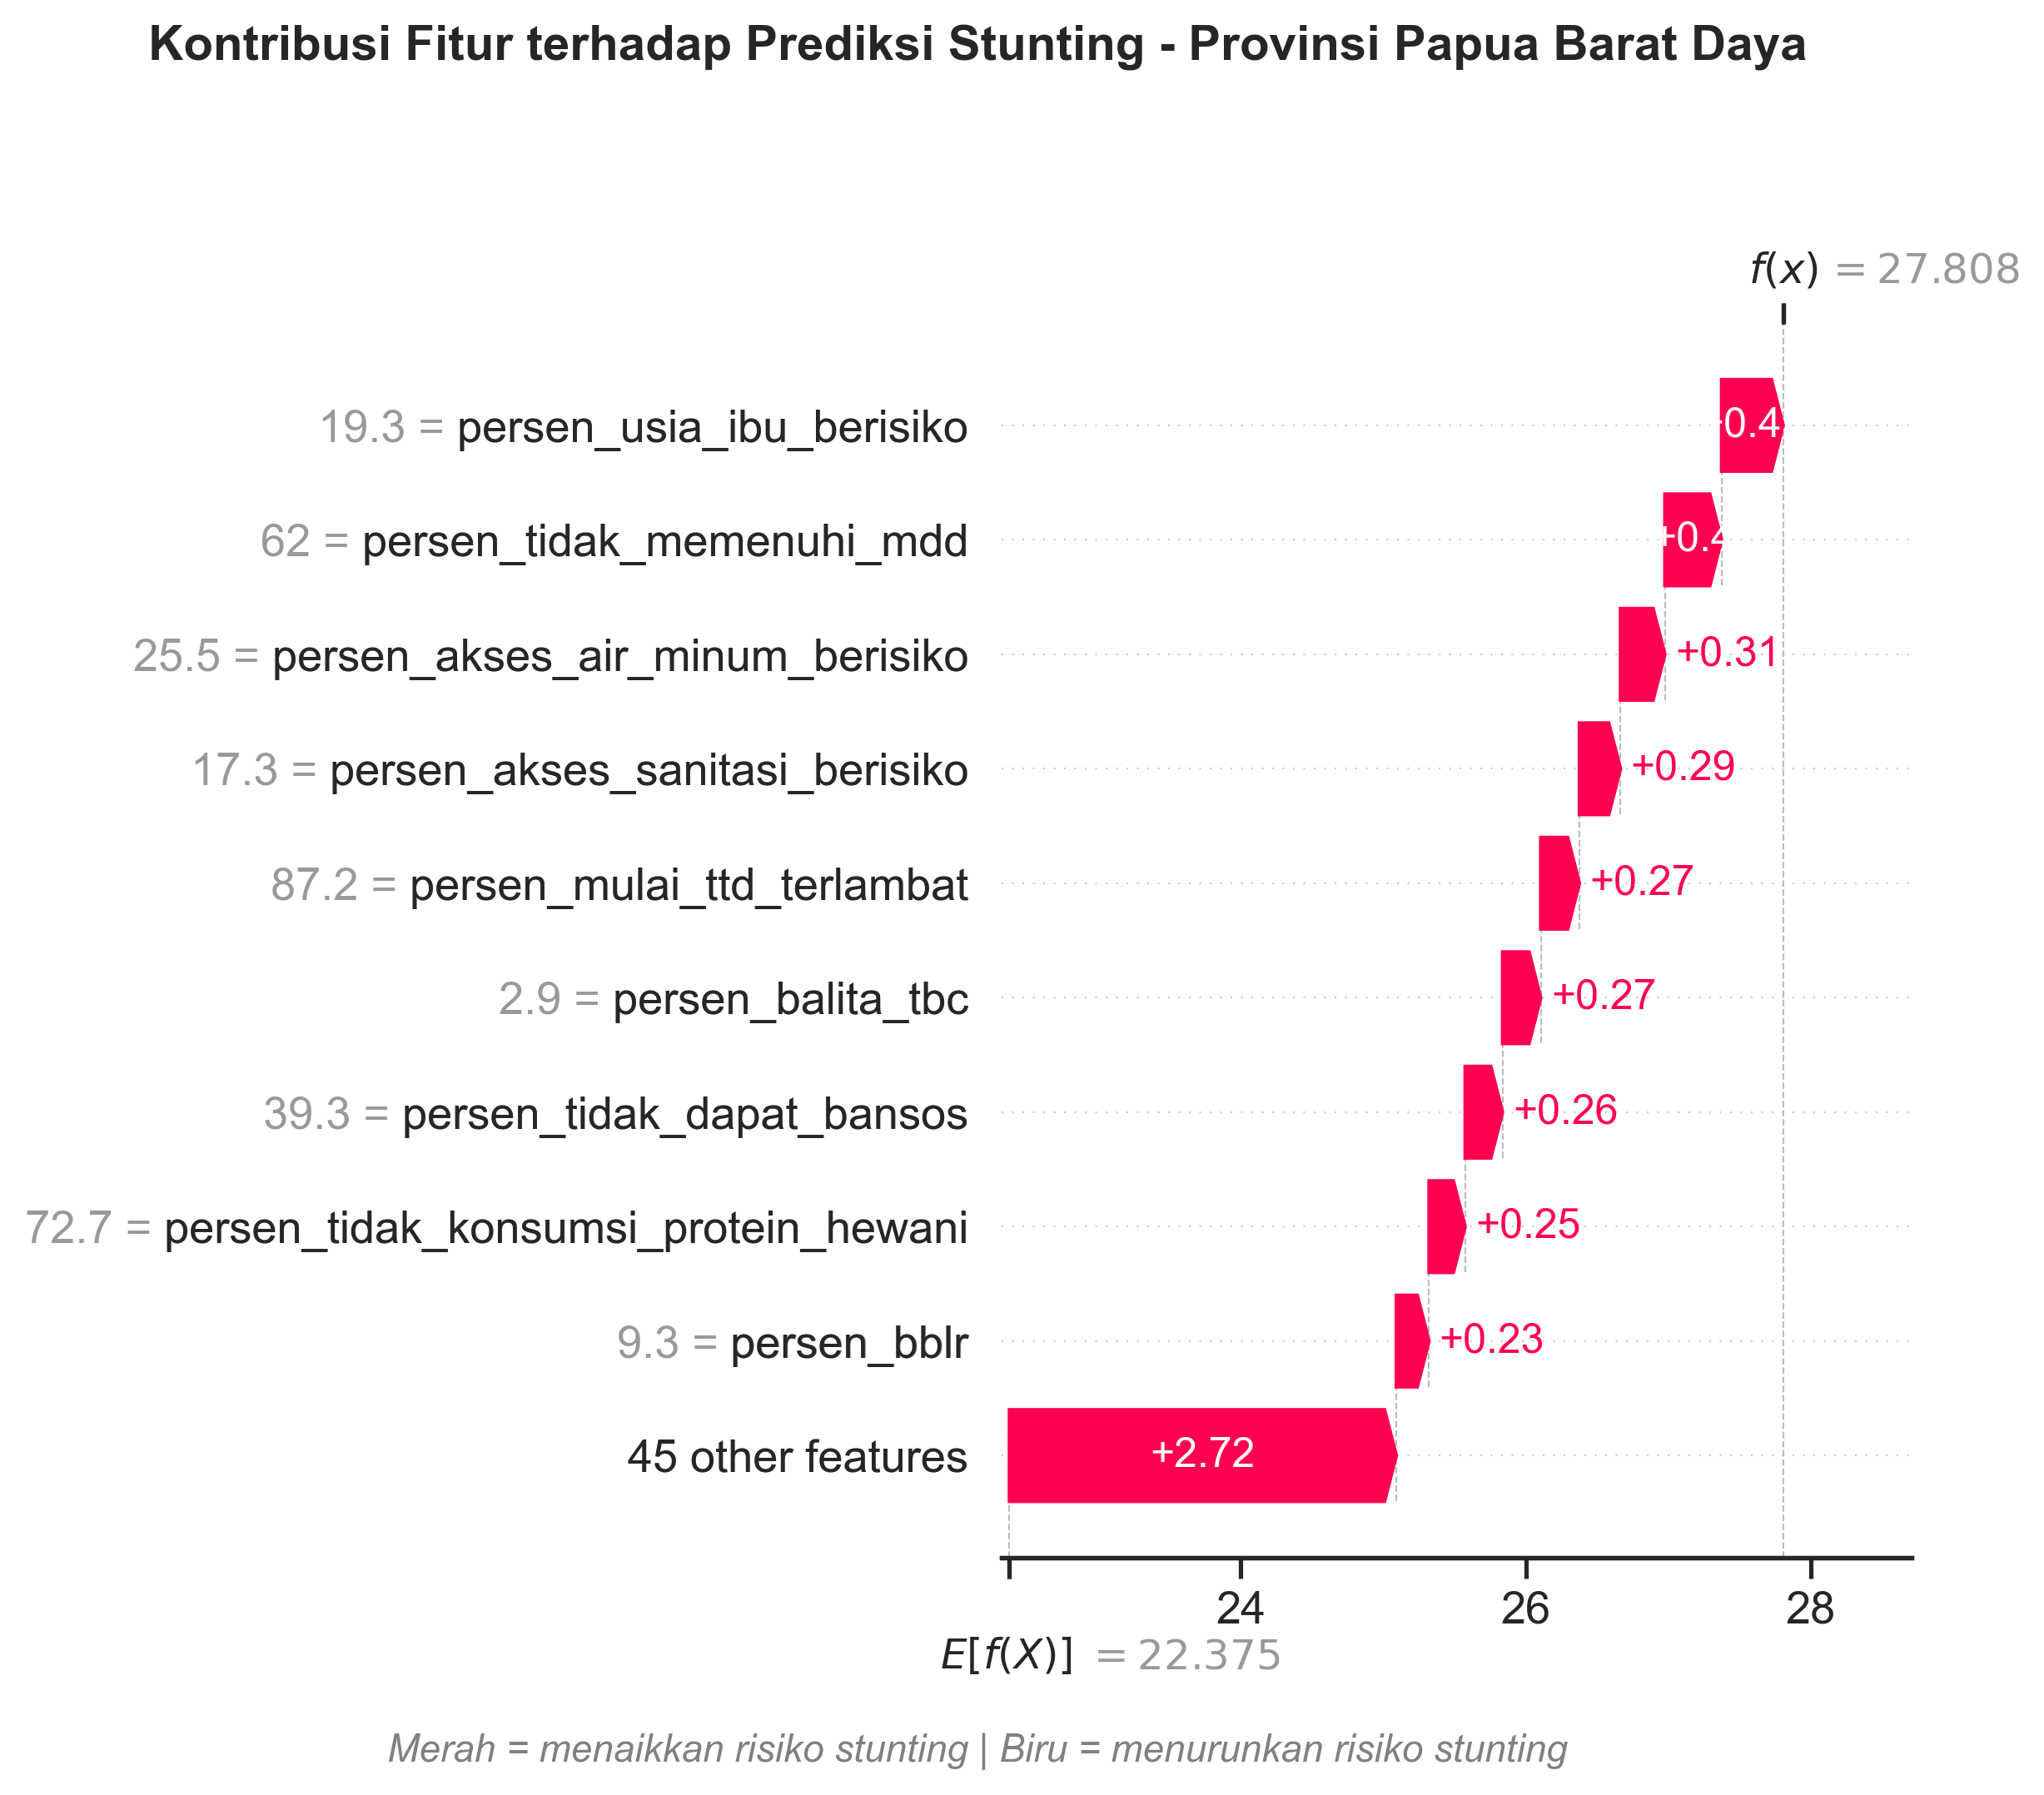
\includegraphics[width=0.48\textwidth]{figure/hasil_waterfall_stunting/waterfall_Papua_Barat_Daya.png} \\ \vspace{0.5cm}
    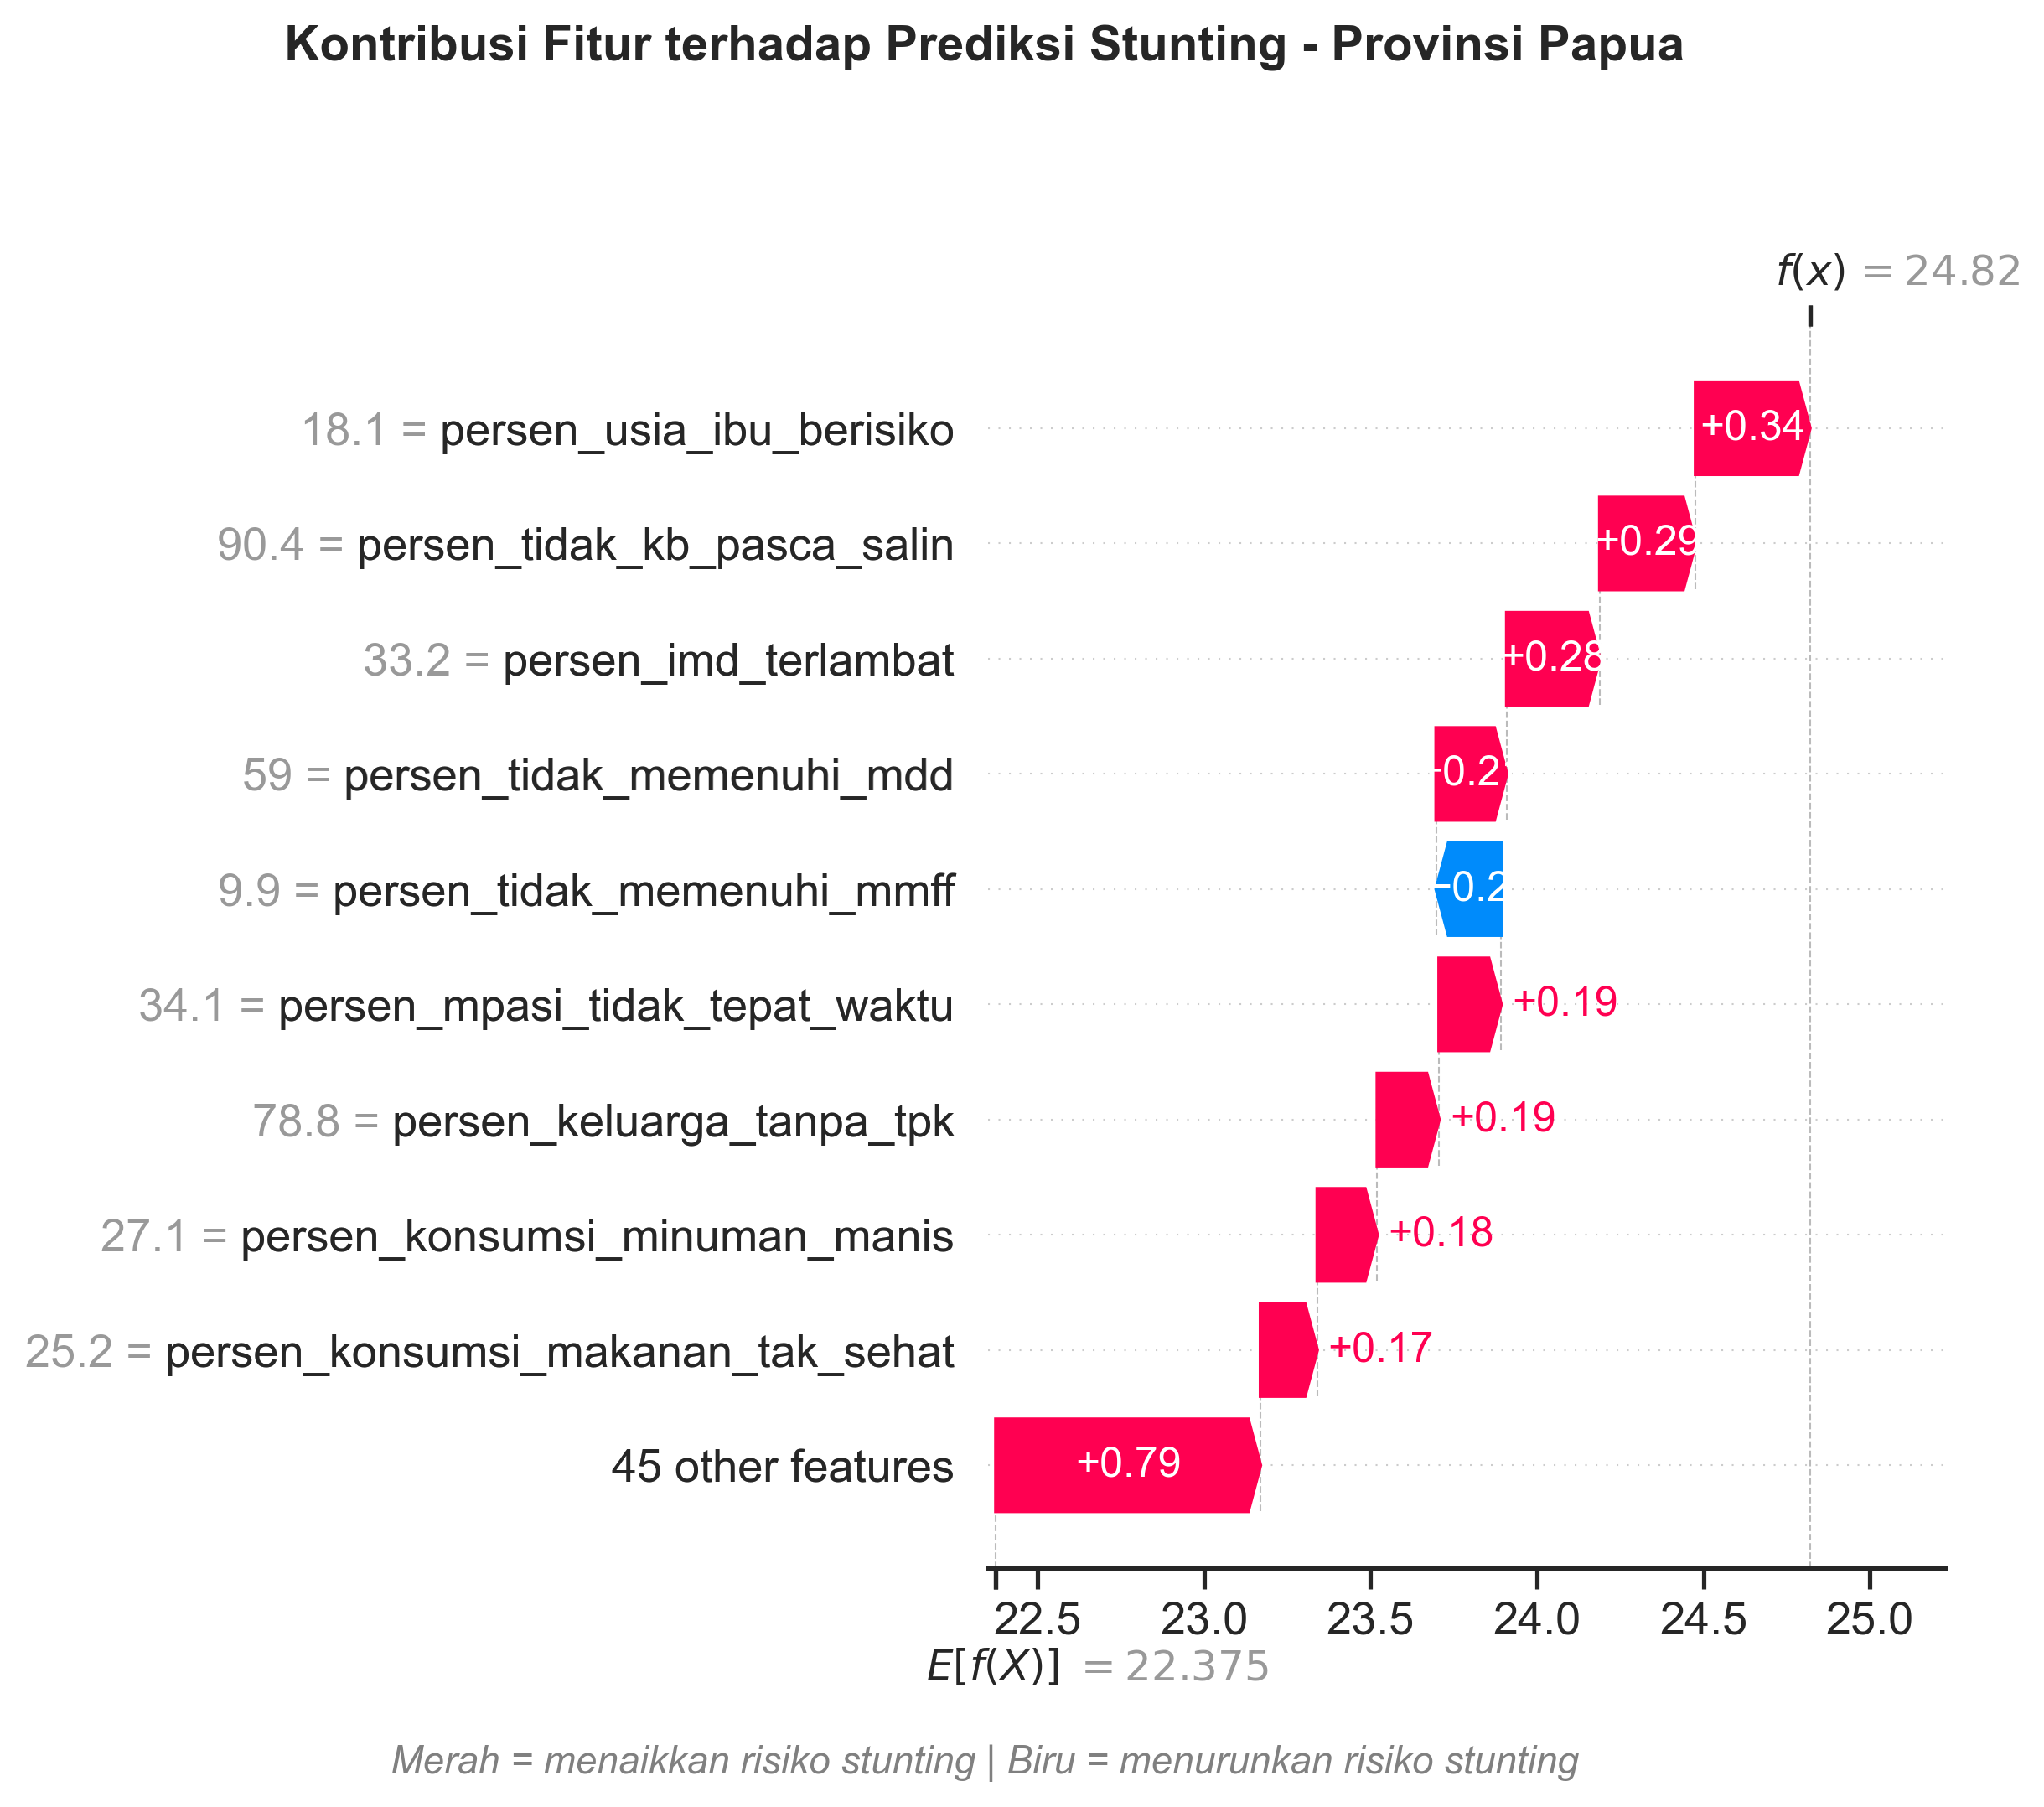
\includegraphics[width=0.48\textwidth]{figure/hasil_waterfall_stunting/waterfall_Papua.png} \hfill
    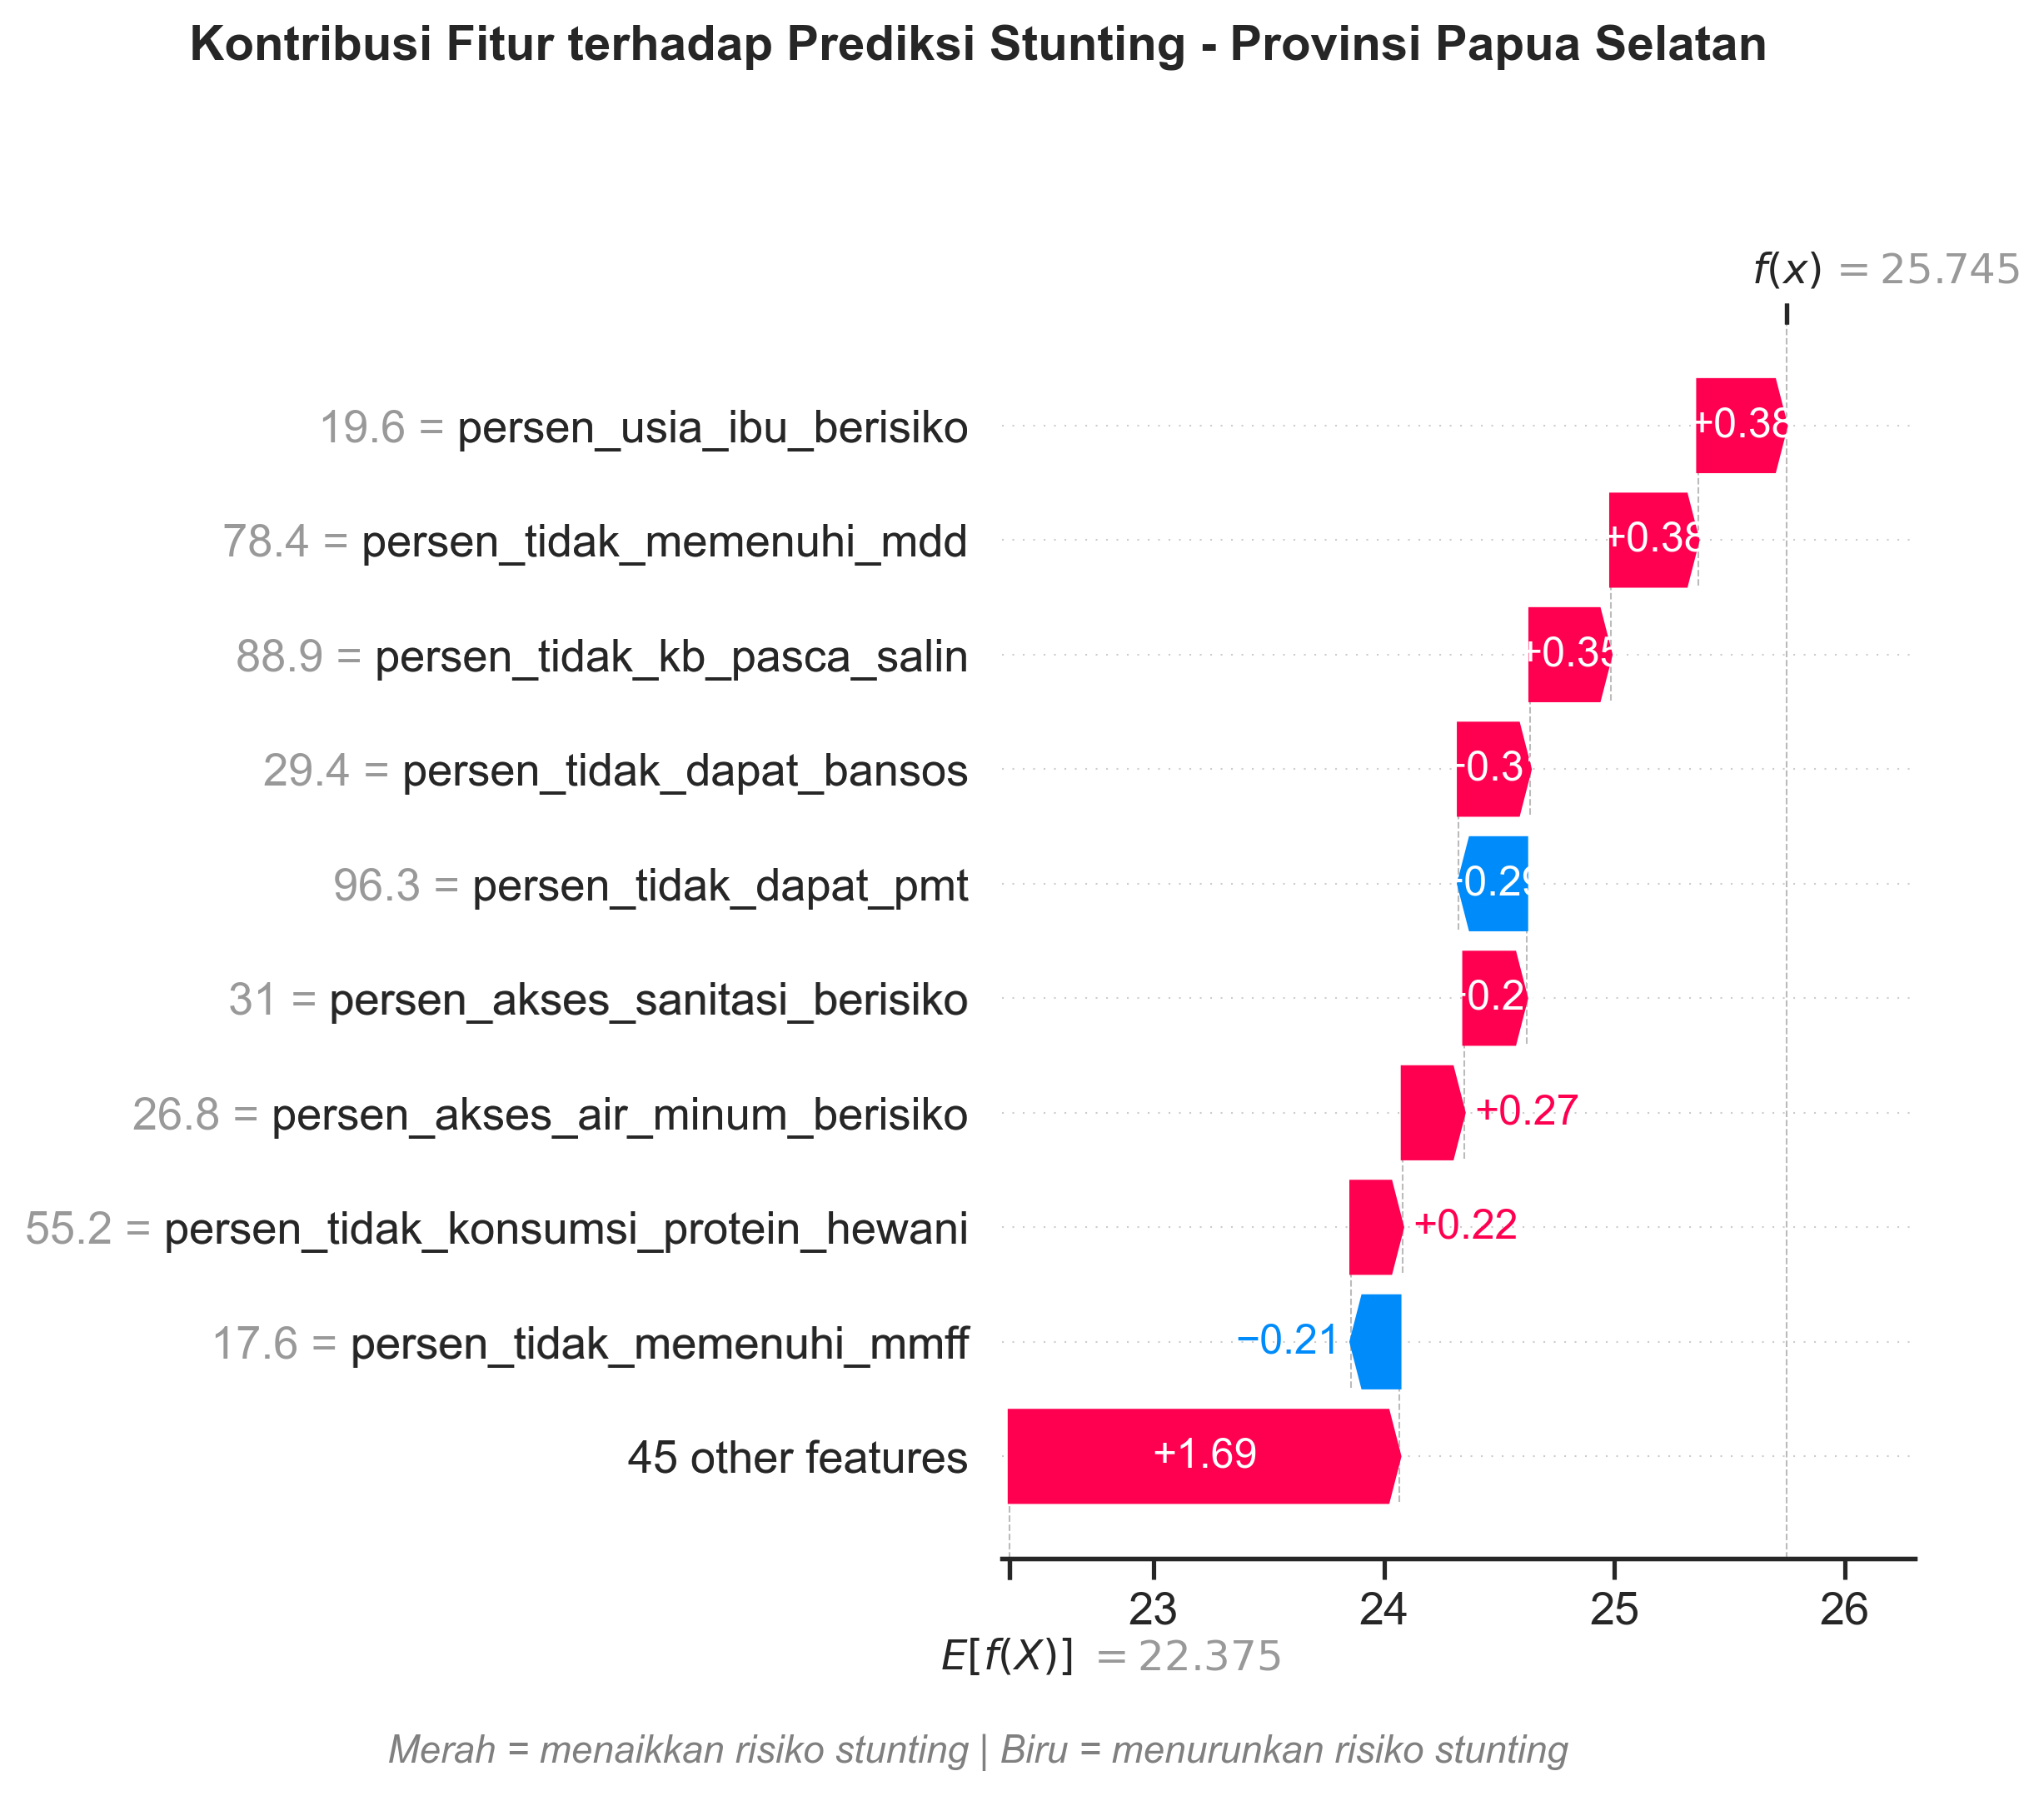
\includegraphics[width=0.48\textwidth]{figure/hasil_waterfall_stunting/waterfall_Papua_Selatan.png}
\end{figure}

